%%%%%%%%%%%%%%%%%%%%%%%%%%%%%%%%%%%%%%%%%%%%%%%%%%%%%%%%%%%%%%%%%%%%%%%%
% Plantilla TFG/TFM
% Escuela Politécnica Superior de la Universidad de Alicante
% Realizado por: Jose Manuel Requena Plens
% Contacto: info@jmrplens.com / Telegram:@jmrplens
%%%%%%%%%%%%%%%%%%%%%%%%%%%%%%%%%%%%%%%%%%%%%%%%%%%%%%%%%%%%%%%%%%%%%%%%

% Elige si deseas optimizar la ejecución del proyecto almacenando las figuras generadas con TikZ y PGF en una carpeta (archivos/figuras-procesadas).
% 1 - Si, 2 - No
\def\OptimizaTikZ{1}

% Archivo .TEX que incluye todas las configuraciones del documento y los paquetes. Añade todo aquello que necesites utilizar en el documento en este archivo.
% En él se encuentra la configuración de los márgenes, establecidos según las directrices de estilo de la EPS.
%%%%%%%%%%%%%%%%%%%%%%%%%%%%%%%%%%%%%%%%%%%%%%%%%%%%%%%%%%%%%%%%%%%%%%%%
% Plantilla TFG/TFM
% Escuela Politécnica Superior de la Universidad de Alicante
% Realizado por: Jose Manuel Requena Plens
% Contacto: info@jmrplens.com / Telegram:@jmrplens
%%%%%%%%%%%%%%%%%%%%%%%%%%%%%%%%%%%%%%%%%%%%%%%%%%%%%%%%%%%%%%%%%%%%%%%%

%%%%%%%%%%%%%%%%%%%%%%%%
% FORMATO DEL DOCUMENTO
%%%%%%%%%%%%%%%%%%%%%%%%
% scrbook es la clase de documento
% Si se desea que no haya página en blanco entre capítulos añadir "openany" en los parámetros de la clase. Sino siempre los capítulos empezarán en página impar.
\documentclass[a4paper,11pt,titlepage]{scrbook}
\KOMAoption{toc}{bib,chapterentryfill} % Opciones del índice
\usepackage{scrhack} % Previene algunos errores
% Paquete de formato para scrbook. Con marcas, linea-separador superior e inferior
\usepackage[automark,headsepline,footsepline]{scrlayer-scrpage}
\clearpairofpagestyles		% Borra los estilos por defecto
%%
% Formato y contenido de la información de cabecera y pie de página
%%
% Información de capítulo en cabecera e interno
\ihead{{\color{gray30}\scshape\small\headmark}}	
% Número de página en cabecera y externo
\ohead{\normalfont\pagemark} 
% Número de página en pie de página y externo. Sólo en páginas sin cabecera
\ofoot[\normalfont\pagemark]{}
%% 		
% Edición del contenido de las distintas partes de la cabecera
%%
\renewcommand{\chaptermark}[1]{\markboth{#1}{}} % Capítulo (Solo texto)
\renewcommand{\sectionmark}[1]{\markright{\thesection. #1}} % Sección (Número y texto)
\setkomafont{pagenumber}{} % Número de página (Sin nada añadido)

% Añade al índice y numera hasta la profundidad 4.
% 1:section,2:subsection,3:subsubsection,4:paragraph
\setcounter{tocdepth}{4}
\setcounter{secnumdepth}{4}
% Muestra una regla para comprobar el formato de las páginas
%\usepackage[type=upperleft,showframe,marklength=8mm]{fgruler}
% MÁRGENES DE LAS PÁGINAS
\usepackage[
  inner	=	3.0cm, % Margen interior
  outer	=	2.5cm, % Margen exterior
  top	=	2.5cm, % Margen superior
  bottom=	2.5cm, % Margen inferior
  includeheadfoot, % Incluye cabecera y pie de página en los márgenes
]{geometry}
% Valor de interlineado
\renewcommand{\baselinestretch}{1.0} % 1 línea de interlineado
% Para poder generar páginas horizontales
\usepackage{lscape}
% Ancho de la zona para comentarios en el margen. (modificado para todonotes)
\setlength{\marginparwidth}{1.9cm}

%%%%%%%%%%%%%%%%%%%%%%%%
% BIBLIOGRAFÍA
%%%%%%%%%%%%%%%%%%%%%%%%
\usepackage{apacite} % NORMA APA
\usepackage{natbib}
\usepackage{breakcites}

%%%%%%%%%%%%%%%%%%%%%%%%
% DOCUMENTO EN ESPAÑOL
%%%%%%%%%%%%%%%%%%%%%%%%
\usepackage[base]{babel}
\usepackage{polyglossia}
\setdefaultlanguage{spanish}

\addto\captionsspanish{%
	\renewcommand{\listtablename}{Índice de tablas} 
	\renewcommand{\tablename}{Tabla}
	\renewcommand{\lstlistingname}{Código}
	\renewcommand{\lstlistlistingname}{Índice de \lstlistingname s}
	\renewcommand{\glossaryname}{Glosario}
	\renewcommand{\acronymname}{Acrónimos}
	\renewcommand{\bibname}{Bibliografía}%
}

%%%%%%%%%%%%%%%%%%%%%%%% 
% COLORES
%%%%%%%%%%%%%%%%%%%%%%%% 
% Biblioteca de colores
\usepackage{color}
\usepackage[dvipsnames]{xcolor}
% Otros colores definidos por el usuario
\definecolor{gray97}{gray}{.97}
\definecolor{gray75}{gray}{.75}
\definecolor{gray45}{gray}{.45}
\definecolor{gray30}{gray}{.30}
\definecolor{negro}{RGB}{0,0,0}
\definecolor{blanco}{RGB}{255,255,255}
\definecolor{dkgreen}{rgb}{0,.6,0}
\definecolor{dkblue}{rgb}{0,0,.6}
\definecolor{dkyellow}{cmyk}{0,0,.8,.3}
\definecolor{gray}{rgb}{0.5,0.5,0.5}
\definecolor{mauve}{rgb}{0.58,0,0.82}
\definecolor{deepblue}{rgb}{0,0,0.5}
\definecolor{deepred}{rgb}{0.6,0,0}
\definecolor{deepgreen}{rgb}{0,0.5,0}
\definecolor{MyDarkGreen}{rgb}{0.0,0.4,0.0}
\definecolor{bluekeywords}{rgb}{0.13,0.13,1}
\definecolor{greencomments}{rgb}{0,0.5,0}
\definecolor{redstrings}{rgb}{0.9,0,0}

%%%%%%%%%%%%%%%%%%%%%%%%
% TABLAS
%%%%%%%%%%%%%%%%%%%%%%%%
% Paquetes para tablas
\usepackage{longtable,booktabs,array,multirow,multicol,tabularx,ragged2e,array}
% Nuevos tipos de columna para tabla, se pueden utilizar como por ejemplo C{3cm} en la definición de columnas de la función tabular
\newcolumntype{L}[1]{>{\raggedright\let\newline\\\arraybackslash\hspace{0pt}}m{#1}}
\newcolumntype{C}[1]{>{\centering\let\newline\\\arraybackslash\hspace{0pt}}m{#1}}
\newcolumntype{R}[1]{>{\raggedleft\let\newline\\\arraybackslash\hspace{0pt}}m{#1}}

%%%%%%%%%%%%%%%%%%%%%%%% 
% GRAFICAS y DIAGRAMAS 
%%%%%%%%%%%%%%%%%%%%%%%% 
% Paquete para todo tipo de gráficas, diagramas, modificación de imágenes, etc
\usepackage{tikz,tikzpagenodes}
\usetikzlibrary{tikzmark,calc,shapes.geometric,arrows,backgrounds,shadings,shapes.arrows,shapes.symbols,shadows,positioning,fit,automata,patterns,intersections}
\usepackage{pgfplots}
\pgfplotsset{colormap/jet}
\pgfplotsset{compat=newest} % Compatibilidad
\usepgfplotslibrary{patchplots,groupplots,fillbetween,polar}
\usepackage{pgfplotstable}
% Guardar las figuras realizadas con Tikz y Pgf en una carpeta externa
% para agilizar el procesado y tenerlas para utilizarlas en otros
% documentos
\if\OptimizaTikZ 1
\usepgfplotslibrary{external}
\tikzexternalize[prefix=archivos/figuras-procesadas/] % Ruta
\tikzset{%
    external/system call ={xelatex -enable-write18 -halt-on-error -interaction=batchmode -jobname "\image" "\texsource"},
}
\fi

% Estilos para elementos graficos
% Cajas y cajas de texto
\tikzstyle{Caja1} = [green,very thick,rounded corners,fill=white, fill opacity=0.5]
\tikzstyle{Texto1} = [fill=white,thick,shape=circle,draw=black,inner sep=2pt,font=\sffamily,text=black]
\tikzstyle{Texto2} = [fill=white,thick,shape=rectangle,draw=black,inner sep=2pt,font=\sffamily,text=black]
\tikzstyle{Texto3} = [fill=white,thick,shape=circle,draw=black,inner sep=2pt,font=\sffamily,text=black]
% Cuadros de diagrama
\tikzstyle{rectvioleta} = [rectangle, rounded corners, text centered, draw=black, fill=blue!10]
\tikzstyle{rectnaranja} = [rectangle, minimum width=2cm, minimum height=1cm, text centered, draw=black, fill=orange!10]
\tikzstyle{romborosa} = [diamond, aspect=3, minimum width=3cm, minimum height=1cm, text centered, draw=black, fill=red!10]
\tikzstyle{rectverde} = [rectangle, minimum width=2cm, minimum height=1cm, text centered, draw=black, fill=green!10]
\tikzstyle{rectamarillo} = [rectangle, rounded corners, minimum width=2cm, minimum height=1cm, text centered, draw=black, fill=yellow!10]
% Flechas
\tikzstyle{arrow} = [thick,->,>=stealth]

%%%%%%%%%%%%%%%%%%%%%%%% 
% FIGURAS, TABLAS, ETC 
%%%%%%%%%%%%%%%%%%%%%%%% 
\usepackage{subcaption} % Para poder realizar subfiguras
\usepackage{caption} % Para aumentar las opciones de diseño
% Nombres de figuras, tablas, etc, en negrita la numeración, todo con letra small
\captionsetup{labelfont={bf,small},textfont=small}
% Paquete para modificar los espacios arriba y abajo de una figura o tabla
\usepackage{setspace}
% Define el espacio tanto arriba como abajo de las figuras, tablas
\setlength{\intextsep}{5mm}
% Para ajustar tamaños de texto de toda una tabla o grafica
% Uso: {\scalefont{0.8} \begin{...} \end{...} }
\usepackage{scalefnt}
% Redefine las tablas y figuras para eliminar el '.' entre la numeración y el texto
\renewcommand*{\figureformat}{\figurename~\thefigure}
\renewcommand*{\tableformat}{\tablename~\thetable}

%%%%%%%%%%%%%%%%%%%%%%%% 
% TEXTO
%%%%%%%%%%%%%%%%%%%%%%%%
% Paquete para poder modificar las fuente de texto
\usepackage{xltxtra}
% Cualquier tamaño de texto. Uso: {\fontsize{100pt}{120pt}\selectfont tutexto}
\usepackage{anyfontsize}
% Para modificar parametros del texto.
\usepackage{setspace}
% Paquete para posicionar bloques de texto
\usepackage{textpos}
% Paquete para realizar cajas de texto. 
% Uso: \begin{mdframed}[linecolor=red!100!black] tutexto \end{mdframed}
\usepackage{framed,mdframed}
% Para subrayar. Uso: \hlc[tucolor]{tutexto}
\newcommand{\hlc}[2][yellow]{ {\sethlcolor{#1} \hl{#2}} }

%%%%%%%%%%%%%%%%%%%%%%%% 
% OTROS
%%%%%%%%%%%%%%%%%%%%%%%%
% Para hacer una pagina horizontal. Uso: \begin{landscape} xxxx \end{lanscape}
\usepackage{lscape} 
% Para incluir paginas PDF. Uso:
% \includepdf[pages={1}]{tuarchivo.pdf}
\usepackage{pdfpages}
% Para introducir url's con formato. Uso: \url{http://www.google.es}
\usepackage{url}
% Amplia muchas funciones graficas de latex
\usepackage{graphicx}
% Paquete que añade el hipervinculo en referencias dentro del documento, indice, etc
% Se define sin bordes alrededor. Uso: \ref{tulabel}
\usepackage[pdfborder={000}]{hyperref}
\usepackage{float}
\usepackage{placeins}
\usepackage{afterpage}
\usepackage{verbatim}
% Paquete para condicionales avanzados
\usepackage{xstring,xifthen}
% Paquete para realizar calculos en el código
\usepackage{calc}
% Para rotar tablas o figuras o su contenido
\usepackage{rotating} 
% Para incluir comentarios en el texto. El parámetro 'disable' oculta todas las notas.
% USO: \todo{tutexto}
\usepackage[textsize=tiny,spanish,shadow,textwidth=2cm]{todonotes}
%\reversemarginpar % Descomentar si se quiere todos los comentarios en el mismo lado
% Desactiva la exportación de los ToDo y Missingfigures como figuras
\if\OptimizaTikZ 1
\makeatletter
\renewcommand{\todo}[2][]{\tikzexternaldisable\@todo[#1]{#2}\tikzexternalenable}
\makeatother
\usepackage{letltxmacro}
\LetLtxMacro{\oldmissingfigure}{\missingfigure}
\makeatletter
\renewcommand{\missingfigure}[2][]{\tikzexternaldisable\oldmissingfigure[{#1}]{#2}\tikzexternalenable}
\makeatother
\fi

%%%%%%%%%%%%%%%%%%%%%%%% 
% GLOSARIOS
%%%%%%%%%%%%%%%%%%%%%%%%
\usepackage[acronym,nonumberlist,toc]{glossaries}
\usepackage{glossary-superragged}
\newglossarystyle{modsuper}{%
  \setglossarystyle{super}%
  \renewcommand{\glsgroupskip}{}
}
\renewcommand{\glsnamefont}[1]{\textbf{#1}}


%%%%%%%%%%%%%%%%%%%%%%%% 
% COMANDOS AÑADIDOS
%%%%%%%%%%%%%%%%%%%%%%%%
% Para mostrar la fecha actual (mes año) con \Hoy
\newcommand{\MES}{%
  \ifcase\month% 0
    \or Enero% 1
    \or Febrero% 2
    \or Marzo% 3
    \or Abril% 4
    \or Mayo% 5
    \or Junio% 6
    \or Julio% 7
    \or Agosto% 8
    \or Septiembre% 9
    \or Octubre% 10
    \or Noviembre% 11
    \or Diciembre% 12
  \fi}
\newcommand{\ANYO}{\number\year}
\newcommand{\Hoy}{\MES\ \ANYO}

%%%%%%%%%%%%%%%%%%%%%%%% 
% MATEMÁTICAS
%%%%%%%%%%%%%%%%%%%%%%%%
\usepackage{mathtools,amsthm,amsfonts,amssymb,bm,mathrsfs,nicefrac,upgreek,bigints} 
% Comando para añadir información de variables a las ecuaciones
% Uso: \begin{condiciones}[donde:] ....... \end{condiciones}
\newenvironment{condiciones}[1][2]
  {%
   #1\tabularx{\textwidth-\widthof{#1}}[t]{
     >{$}l<{$} @{}>{${}}c<{{}$}@{} >{\raggedright\arraybackslash}X
   }%
  }
  {\endtabularx\\[\belowdisplayskip]}

%%%%%
% PARÁMETROS DE FORMATO DE CODIGOS
%%%%%
% Puedes editar los formatos para ajustarlos a tu gusto
%%%%%%%%%%%%%%%%%%%%%%%%%%%%%%%%%%%%%%%%%%%%%%%%%%%%%%%%%%%%%%%%%%%%%%%%
% Plantilla TFG/TFM
% Escuela Politécnica Superior de la Universidad de Alicante
% Realizado por: Jose Manuel Requena Plens
% Contacto: info@jmrplens.com / Telegram:@jmrplens
%%%%%%%%%%%%%%%%%%%%%%%%%%%%%%%%%%%%%%%%%%%%%%%%%%%%%%%%%%%%%%%%%%%%%%%%


%%%%%%%%%%%%%%%%%%%%%%%% 
% CÓDIGO. CONFIGURACIÓN. En el siguiente bloque están los estilos.
%%%%%%%%%%%%%%%%%%%%%%%%
% Paquete para mostrar código de matlab. En caja y lineas numeradas
\usepackage[framed,numbered]{matlab-prettifier}
% Paquete mostrar código de programación de distintos lenguajes
\usepackage{listings}
\lstset{ inputencoding=utf8,
extendedchars=true,
frame=single, % Caja donde se ubica el código
backgroundcolor=\color{gray97}, % Color del fondo de la caja
rulesepcolor=\color{black},
boxpos=c,
abovecaptionskip=-4pt,
aboveskip=12pt,
belowskip=0pt,
lineskip=0pt,
framerule=0pt,
framextopmargin=4pt,
framexbottommargin=4pt,
framexleftmargin=11pt,
framexrightmargin=0pt,
linewidth=\linewidth,
xleftmargin=\parindent,
framesep=0pt,
rulesep=.4pt,
stringstyle=\ttfamily,
showstringspaces = false,
showspaces = false,
showtabs = false,
columns=fullflexible,
basicstyle=\small\ttfamily,
commentstyle=\color{gray45},
keywordstyle=\bfseries,
tabsize=4,
numbers=left,
numbersep=1pt,
numberstyle=\tiny\ttfamily\color{gray75},
numberfirstline = false,
breaklines=true,
postbreak=\mbox{\textcolor{red}{$\hookrightarrow$}\space}, % Flecha al saltar de linea
prebreak=\mbox{\textcolor{red}{$\hookleftarrow$}\space}, % Flecha al saltar de linea
literate=
  {á}{{\'a}}1 {é}{{\'e}}1 {í}{{\'i}}1 {ó}{{\'o}}1 {ú}{{\'u}}1
  {Á}{{\'A}}1 {É}{{\'E}}1 {Í}{{\'I}}1 {Ó}{{\'O}}1 {Ú}{{\'U}}1
  {à}{{\`a}}1 {è}{{\`e}}1 {ì}{{\`i}}1 {ò}{{\`o}}1 {ù}{{\`u}}1
  {À}{{\`A}}1 {È}{{\'E}}1 {Ì}{{\`I}}1 {Ò}{{\`O}}1 {Ù}{{\`U}}1
  {ä}{{\"a}}1 {ë}{{\"e}}1 {ï}{{\"i}}1 {ö}{{\"o}}1 {ü}{{\"u}}1
  {Ä}{{\"A}}1 {Ë}{{\"E}}1 {Ï}{{\"I}}1 {Ö}{{\"O}}1 {Ü}{{\"U}}1
  {â}{{\^a}}1 {ê}{{\^e}}1 {î}{{\^i}}1 {ô}{{\^o}}1 {û}{{\^u}}1
  {Â}{{\^A}}1 {Ê}{{\^E}}1 {Î}{{\^I}}1 {Ô}{{\^O}}1 {Û}{{\^U}}1
  {œ}{{\oe}}1 {Œ}{{\OE}}1 {æ}{{\ae}}1 {Æ}{{\AE}}1 {ß}{{\ss}}1
  {ű}{{\H{u}}}1 {Ű}{{\H{U}}}1 {ő}{{\H{o}}}1 {Ő}{{\H{O}}}1
  {ç}{{\c c}}1 {Ç}{{\c C}}1 {ø}{{\o}}1 {å}{{\r a}}1 {Å}{{\r A}}1
  {€}{{\euro}}1 {£}{{\pounds}}1 {«}{{\guillemotleft}}1
  {»}{{\guillemotright}}1 {ñ}{{\~n}}1 {Ñ}{{\~N}}1 {¿}{{?`}}1,
  }

% Intenta no dividir los códigos en diferentes paginas si es posible
\lstnewenvironment{listing}[1][]
   {\lstset{#1}\pagebreak[0]}{\pagebreak[0]}

% Formato de títulos de los códigos
\DeclareCaptionFont{white}{\color{white}}
\DeclareCaptionFormat{listing}{\colorbox{gray}{\parbox{\textwidth - 2\fboxsep}{#1#2#3}}}
\captionsetup[lstlisting]{format=listing,labelfont=white,textfont=white,font= scriptsize}


%%%%%%%%%%%%%%%%%%%%%%%% 
% CÓDIGO. ESTILOS. Ajústalos a tu gusto
%%%%%%%%%%%%%%%%%%%%%%%%
\lstdefinestyle{Consola}
	{
	basicstyle=\scriptsize\bf\ttfamily,
	}
   
\lstdefinestyle{C}
	{
	basicstyle=\scriptsize,
	language=C,
	}
\lstdefinestyle{C-color}
	{
  	breaklines=true,
  	language=C,
  	basicstyle=\scriptsize,
  	keywordstyle=\bfseries\color{green!40!black},
  	commentstyle=\itshape\color{purple!40!black},
  	identifierstyle=\color{blue},
  	stringstyle=\color{orange},
    }
\lstdefinestyle{CSharp}
	{
	basicstyle=\scriptsize
	language=[Sharp]C,
	escapeinside={(*@}{@*)},
	keywordstyle=\bfseries,
	}
\lstdefinestyle{CSharp-color}
	{
	basicstyle=\scriptsize
	language=[Sharp]C,
	escapeinside={(*@}{@*)},
	commentstyle=\color{greencomments},
	keywordstyle=\color{bluekeywords}\bfseries,
	stringstyle=\color{redstrings},
	}
\lstdefinestyle{C++}
	{
	basicstyle=\scriptsize,
	language=C++,
 	}
 	
\lstdefinestyle{C++-color}
	{
  	breaklines=true,
  	language=C++,
  	basicstyle=\scriptsize,
  	keywordstyle=\bfseries\color{green!40!black},
  	commentstyle=\itshape\color{purple!40!black},
  	identifierstyle=\color{blue},
  	stringstyle=\color{orange},
    }
    
\lstdefinestyle{PHP}
	{
	basicstyle=\scriptsize,
	language=PHP,
	}
	
\lstdefinestyle{PHP-color}
	{
	basicstyle=\scriptsize,
	language=PHP,
	keywordstyle    = \color{dkblue},
  	stringstyle     = \color{red},
  	identifierstyle = \color{dkgreen},
  	commentstyle    = \color{gray},
  	emph            =[1]{php},
  	emphstyle       =[1]\color{black},
  	emph            =[2]{if,and,or,else},
  	emphstyle       =[2]\color{dkyellow}
  }
  
\lstdefinestyle{Matlab}
	{
	basicstyle=\scriptsize,
	language=Matlab,
	numberstyle=\tiny\ttfamily\color{gray75},
	}
	
\lstdefinestyle{Matlab-color}
	{
	style = Matlab-editor,
	basicstyle=\scriptsize,
	numberstyle=\tiny\ttfamily\color{gray75},
	}
	
\lstdefinestyle{Latex}
	{
	language=[LaTeX]{Tex},
    basicstyle=\scriptsize,
    literate={\$}{{{\bfseries\$}}}1,
    alsoletter={\\,*,\&},
    emph =[1]{\\begin,\\end,\\caption,\\label,\\centering,\\FloatBarrier,
              \\lstinputlisting,\\scalefont,\\addplot,\\input,
              \\legend,\\item,\\subitem,\\includegraphics,\\textwidth,
              \\section,\\subsection,\\subsubsection,\\paragraph,
              \\cite,\\citet,\\citep,\\gls,\\bibliographystyle,\\url,
              \\citet*,\\citep*,\\todo,\\missingfigure,\\footnote},
  	emphstyle =[1]\bfseries,
  	emph = [2]{equation,subequations,eqnarray,figure,subfigure,
  			   condiciones,flalign,tikzpicture,axis,lstlisting,
  			   itemize,description
  			   },
  	emphstyle =[2]\bfseries,
    numbers=none,
	}
	
\lstdefinestyle{Latex-color}
	{
	language=[LaTeX]{Tex},
    basicstyle=\scriptsize,
    commentstyle=\color{dkgreen},
    identifierstyle=\color{black},
    literate={\$}{{{\bfseries\color{Dandelion}\$}}}1, % Colorea el simbolo dollar
    alsoletter={\\,*,\&},
    emph =[1]{\\begin,\\end,\\caption,\\label,\\centering,\\FloatBarrier,
              \\lstinputlisting,\\scalefont,\\addplot,\\input,
              \\legend,\\item,\\subitem,\\includegraphics,\\textwidth,
              \\section,\\subsection,\\subsubsection,\\paragraph,
              \\cite,\\citet,\\citep,\\gls,\\bibliographystyle,\\url,
              \\citet*,\\citep*,\\todo,\\missingfigure,\\footnote},
  	emphstyle =[1]\bfseries\color{RoyalBlue},
  	emph = [2]{equation,subequations,eqnarray,figure,subfigure,
  			   condiciones,flalign,tikzpicture,axis,lstlisting,
  			   itemize,description
  			   },
  	emphstyle =[2]\bfseries,
    numbers=none,
	}
\lstdefinestyle{Java}
{
	basicstyle=\scriptsize,
	language=Java,
}

\lstdefinestyle{Java-color}
{
	basicstyle=\scriptsize,
	language=Java,
  	keywordstyle=\color{blue},
  	commentstyle=\color{dkgreen},
  	stringstyle=\color{mauve},
}
\lstdefinestyle{Python}
{
	language=Python,
	basicstyle=\scriptsize,
	otherkeywords={self},  
	keywordstyle=\bfseries,     
	emphstyle=\bfseries,    
	emph={MyClass,__init__},         
}

\lstdefinestyle{Python-color}
{
	language=Python,
	basicstyle=\scriptsize,
	otherkeywords={self},          
	keywordstyle=\bfseries\color{deepblue},
	emph={MyClass,__init__},         
	emphstyle=\bfseries\color{deepred},    
	stringstyle=\color{deepgreen},
}
\lstdefinestyle{R}
{
	language=R,                     
  	basicstyle=\scriptsize,
  	keywordstyle=\bfseries, 
}
\lstdefinestyle{R-color}
{
	language=R,                     
  	basicstyle=\scriptsize,
  	keywordstyle=\bfseries\color{RoyalBlue}, 
  	commentstyle=\color{YellowGreen},
  	stringstyle=\color{ForestGreen}  
}


%%%%%
% DEFINICION DE CONCEPTOS
%%%%
% Uso ejemplo: \begin{ejemplo} tucontenido \end{ejemplo} 
\newtheorem{teorema}{Teorema}[chapter]
\newtheorem{ejemplo}{Ejemplo}[chapter]
\newtheorem{definicion}{Definición}[chapter]



%%%%%%%%%%%%%%%%%%%%%%%%%%%%%%%%%%%%%%%%%%%%%%%%%%%%%%%%%%%%%%%%%%%%%%
% INFORMACIÓN DEL TFG
% Comentar lo que NO se desee añadir y sustituir con la información correcta.
%%%%%%%%%%%%%%%%%%%%%%%%%%%%%%%%%%%%%%%%%%%%%%%%%%%%%%%%%%%%%%%%%%%%%%
% Título y subtítulo
\newcommand{\titulo}{Desarrollo de una arquitectura hardware para procesamiento especializado}
\newcommand{\subtitulo}{Basado en CORDIC}
% Datos del autor
\newcommand{\miNombre}{Vladyslav Korkoshko Tereshchenko}
\newcommand{\miEmail}{vk21@alu.ua.es}
% Datos del tutor/es
\newcommand{\miTutor}{Marcelo Saval Calvo}
\newcommand{\miTutorB}{Jose Luís Sánchez Romero}
\newcommand{\departamentoTutor}{Tecnología Informática y Computación}
\newcommand{\departamentoTutorB}{Tecnología Informática y Computación}
% Datos de la facultada y universidad
\newcommand{\miFacultad}{Escuela Politécnica Superior}
\newcommand{\miFacultadCorto}{EPS UA}
\newcommand{\miUniversidad}{\protect{Universidad de Alicante}}
\newcommand{\miUbicacion}{Alicante}

%%%%%%%%%%%%%%%%%%%%%%%%%%%%%%%%%%%%%%%%%%%%%%%%%%%%%%%%%%%%%%%%%%%%%%
% INDICA TU TITULACIÓN
% ID	GRADO -------------------------------------------------
% 1		Ingeniería en Imagen y Sonido en Telecomunicación
% 2		Ingeniería Civil
% 3		Ingeniería Química
% 4		Ingeniería Informática
% 5		Ingeniería Multimedia
% 6		Arquitectura Técnica
% 7		Arquitectura
% 8		Robótica
% %		%%%%%%%%%%%%
% ID	MÁSTER ------------------------------------------------
% A		Telecomunicación
% B		Caminos, Canales y Puertos
% C		Gestión en la Edificación
% D		Desarrollo Web
% E		Materiales, Agua, Terreno
% F		Informática
% G 	Automática y Robótica
% H		Prevención de riesgos laborales
% I		Gestión Sostenible Agua
% J		Desarrollo Aplicaciones Móviles
% K		Ingeniería Química
%%%%%%%%%%%%%%%%%%%%%%%%%%%%%%%%%%%%%%%%%%%%%%%%%%%%%%%%%%%%%%%%%%%%%%%%%
%!!!!!!!!!!!!!!!!!!!!!!!!!!!!!!!!!!!!!!!!!!!!!!!!!!!!!!!!!!!!!!!!!!!!!%%%
																		%
\def\IDtitulo{4} % INTRODUCE LA ID DE TU TITULACIÓN						%
																		%
%!!!!!!!!!!!!!!!!!!!!!!!!!!!!!!!!!!!!!!!!!!!!!!!!!!!!!!!!!!!!!!!!!!!!!%%%
%%%%%%%%%%%%%%%%%%%%%%%%%%%%%%%%%%%%%%%%%%%%%%%%%%%%%%%%%%%%%%%%%%%%%%%%%

% Configuración automática según el identificador elegido
%%%%%%%%%%%%%%%%%%%%%%%%%%%%%%%%%%%%%%%%%%%%%%%%%%%%%%%%%%%%%%%%%%%%%%%%
% Plantilla TFG/TFM
% Escuela Politécnica Superior de la Universidad de Alicante
% Realizado por: Jose Manuel Requena Plens
% Contacto: info@jmrplens.com / Telegram:@jmrplens
%%%%%%%%%%%%%%%%%%%%%%%%%%%%%%%%%%%%%%%%%%%%%%%%%%%%%%%%%%%%%%%%%%%%%%%%

%%%%%%%%%%%%%%%%%%%%%%%% 
% COLORES DE GRADOS.
% Si el color de la titulación ha cambiado, modifícalo en las lineas siguientes.
%%%%%%%%%%%%%%%%%%%%%%%%
% Grados
\definecolor{teleco}{RGB}{32,2,116}			% Teleco
\definecolor{civil}{RGB}{201,56,140}			% Civil
\definecolor{quimica}{RGB}{41,199,255}		% Química
\definecolor{informatica}{RGB}{0,128,255}	% Informatica
\definecolor{multimedia}{RGB}{239,206,53}	% Multimedia
\definecolor{arquitecnica}{RGB}{0,179,148}	% Arquitectura técnica
\definecolor{arquitectura}{RGB}{181,0,0}		% Arquitectura
\definecolor{robotica}{RGB}{0,128,255}		% Robótica
% Másteres
\definecolor{masterteleco}{RGB}{32,2,116}	% Teleco
\definecolor{caminos}{RGB}{201,56,140}		% Caminos, Canales y Puertos
\definecolor{gestedif}{RGB}{50,120,50}		% Gestión Edificación
\definecolor{desweb}{RGB}{250,43,22}			% Desarrollo Web
\definecolor{mataguaterre}{RGB}{210,250,50}	% Materiales, Agua, Terreno
\definecolor{masterinfor}{RGB}{0,128,255}	% Informática
\definecolor{autorobo}{RGB}{83,145,201}		% Automática y Robótica
\definecolor{prevencion}{RGB}{0,100,0}		% Prevención Riesgos
\definecolor{gestionagua}{RGB}{7,138,197}	% Gestión Agua
\definecolor{moviles}{RGB}{121,11,21}		% Aplicaciones Móviles
\definecolor{masterquimica}{RGB}{41,199,255}	% Aplicaciones Móviles

% Logotipos comunes de todas las titulaciones
\newcommand{\logoFacultad}{include/logos-universidad/LogoEPSNegro}
\newcommand{\logoUniversidad}{include/logos-universidad/LogoUANegro}
\newcommand{\logoUniversidadPortada}{include/logos-universidad/LogoUABlanco}

% Colores generales
\definecolor{negro}{RGB}{0,0,0}
\definecolor{blanco}{RGB}{255,255,255}
%%%%%%%%%%%%%%%%%%%%%%%% 
% CONDICIONALES. SEGUN LA ID ELEGIDA EN EL .TEX PRINCIPAL
% Según el ID seleccionado en TFG_EPS_UA.tex se configurará el nombre de la titulación, logotipos y color.
% Si tu titulación no esta correctamente definida cambia las imágenes que se definen para tu titulación en las lineas de abajo
% Si deseas añadir mas titulaciones ve al final de este archivo
%%%%%%%%%%%%%%%%%%%%%%%%
% Grados
	\if\IDtitulo 1 % Teleco
		% Logos
		\newcommand{\logoFacultadPortada}{include/logos-universidad/LogoEPSBlanco}
		\newcommand{\logoGradoPortada}{include/logos-titulaciones/LogoTelecoBlanco}
		\newcommand{\logoGrado}{include/logos-titulaciones/LogoTelecoNegro}
		% Texto
		\newcommand{\miGrado}{Grado en Ingeniería en Sonido e Imagen en Telecomunicación}
		\newcommand{\tipotrabajo}{Trabajo Fin de Grado}
		% Color
		\newcommand{\colorgrado}{teleco}
		\newcommand{\colortexto}{blanco}
	\else \if\IDtitulo 2 % Civil
		\newcommand{\logoFacultadPortada}{include/logos-universidad/LogoEPSBlanco}
		\newcommand{\logoGradoPortada}{include/logos-titulaciones/LogoCivilBlanco}
		\newcommand{\logoGrado}{include/logos-titulaciones/LogoCivilNegro}
		% Texto
		\newcommand{\miGrado}{Grado en Ingeniería Civil}
		\newcommand{\tipotrabajo}{Trabajo Fin de Grado}
		% Color
		\newcommand{\colorgrado}{civil}
		\newcommand{\colortexto}{blanco}
	\else \if\IDtitulo 3 % Quimica
		% Logos
		\newcommand{\logoFacultadPortada}{include/logos-universidad/LogoEPSNegro}
		\newcommand{\logoGradoPortada}{include/logos-titulaciones/LogoQuimicaNegro}
		\newcommand{\logoGrado}{include/logos-titulaciones/LogoQuimicaNegro}
		% Texto
		\newcommand{\miGrado}{Grado en Ingeniería Química}
		\newcommand{\tipotrabajo}{Trabajo Fin de Grado}
		% Color
		\newcommand{\colorgrado}{quimica}
		\newcommand{\colortexto}{negro}
	\else \if\IDtitulo 4 % Informatica
		% Logos
		\newcommand{\logoFacultadPortada}{include/logos-universidad/LogoEPSBlanco}
		\newcommand{\logoGradoPortada}{include/logos-titulaciones/LogoInformaticaBlanco}
		\newcommand{\logoGrado}{include/logos-titulaciones/LogoInformaticaNegro}
		% Texto
		\newcommand{\miGrado}{Grado en Ingeniería Informática}
		\newcommand{\tipotrabajo}{Trabajo Fin de Grado}
		% Color
		\newcommand{\colorgrado}{informatica}
		\newcommand{\colortexto}{blanco}
	\else \if\IDtitulo 5 % Multimedia
		% Logos
		\newcommand{\logoFacultadPortada}{include/logos-universidad/LogoEPSNegro}
		\newcommand{\logoGradoPortada}{include/logos-titulaciones/LogoMultimediaNegro}
		\newcommand{\logoGrado}{include/logos-titulaciones/LogoMultimediaNegro}
		% Texto
		\newcommand{\miGrado}{Grado en Ingeniería Multimedia}
		\newcommand{\tipotrabajo}{Trabajo Fin de Grado}
		% Color
		\newcommand{\colorgrado}{multimedia}
		\newcommand{\colortexto}{negro}
	\else \if\IDtitulo 6 % Arquitectura Tecnica
		% Logos
		\newcommand{\logoFacultadPortada}{include/logos-universidad/LogoEPSBlanco}
		\newcommand{\logoGradoPortada}{include/logos-titulaciones/LogoArqTecnicaBlanco}
		\newcommand{\logoGrado}{include/logos-titulaciones/LogoArqTecnicaNegro}
		% Texto
		\newcommand{\miGrado}{Grado en Arquitectura Técnica}
		\newcommand{\tipotrabajo}{Trabajo Fin de Grado}
		% Color
		\newcommand{\colorgrado}{arquitecnica}
		\newcommand{\colortexto}{blanco}
	\else \if\IDtitulo 7 % Arquitectura
		% Logos
		\newcommand{\logoFacultadPortada}{include/logos-universidad/LogoEPSBlanco}
		\newcommand{\logoGradoPortada}{include/logos-titulaciones/LogoArquitecturaBlanco}
		\newcommand{\logoGrado}{include/logos-titulaciones/LogoArquitecturaNegro}
		% Texto
		\newcommand{\miGrado}{Grado en Arquitectura}
		\newcommand{\tipotrabajo}{Trabajo Fin de Grado}
		% Color
		\newcommand{\colorgrado}{arquitectura}
		\newcommand{\colortexto}{blanco}
	\else \if\IDtitulo 8 % Robotica
		% Logos
		\newcommand{\logoFacultadPortada}{include/logos-universidad/LogoEPSBlanco}
		\newcommand{\logoGradoPortada}{include/logos-titulaciones/LogoInformaticaBlanco}
		\newcommand{\logoGrado}{include/logos-titulaciones/LogoInformaticaNegro}
		% Texto
		\newcommand{\miGrado}{Grado en Ingeniería Robótica}
		\newcommand{\tipotrabajo}{Trabajo Fin de Grado}
		% Color
		\newcommand{\colorgrado}{robotica}
		\newcommand{\colortexto}{blanco}
% Másteres
	\else \if\IDtitulo A % Teleco
		% Logos
		\newcommand{\logoFacultadPortada}{include/logos-universidad/LogoEPSBlanco}
		\newcommand{\logoGradoPortada}{include/logos-titulaciones/LogoTelecoBlanco}
		\newcommand{\logoGrado}{include/logos-titulaciones/LogoTelecoNegro}
		% Texto
		\newcommand{\miGrado}{Máster Universitario en Ingeniería en Telecomunicación}
		\newcommand{\tipotrabajo}{Trabajo Fin de Máster}
		% Color
		\newcommand{\colorgrado}{masterteleco}
		\newcommand{\colortexto}{blanco}
	\else \if\IDtitulo B % Caminos, Canales y puertos
		% Logos
		\newcommand{\logoFacultadPortada}{include/logos-universidad/LogoEPSBlanco}
		\newcommand{\logoGradoPortada}{include/logos-titulaciones/LogoCivilBlanco}
		\newcommand{\logoGrado}{include/logos-titulaciones/LogoCivilNegro}
		% Texto
		\newcommand{\miGrado}{Máster Universitario en Ingeniería de Caminos, Canales y Puertos}
		\newcommand{\tipotrabajo}{Trabajo Fin de Máster}
		% Color
		\newcommand{\colorgrado}{caminos}
		\newcommand{\colortexto}{blanco}
	\else \if\IDtitulo C % Gestión Edificación
		% Logos
		\newcommand{\logoFacultadPortada}{include/logos-universidad/LogoEPSBlanco}
		\newcommand{\logoGradoPortada}{include/logos-titulaciones/LogoMasterEdificacionBlanco}
		\newcommand{\logoGrado}{include/logos-titulaciones/LogoMasterEdificacionNegro}
		\newcommand{\tipotrabajo}{Trabajo Fin de Máster}
		% Texto
		\newcommand{\miGrado}{Máster Universitario en Gestión de la Edificación}
		% Color
		\newcommand{\colorgrado}{gestedif}
		\newcommand{\colortexto}{blanco}
	\else \if\IDtitulo D % Desarrollo web
		% Logos
		\newcommand{\logoFacultadPortada}{include/logos-universidad/LogoEPSBlanco}
		\newcommand{\logoGradoPortada}{include/logos-titulaciones/LogoMasterDesarrolloBlanco}
		\newcommand{\logoGrado}{include/logos-titulaciones/LogoMasterDesarrolloNegro}
		% Texto
		\newcommand{\miGrado}{Máster Universitario en Desarrollo de Aplicaciones y Servicios Web}
		\newcommand{\tipotrabajo}{Trabajo Fin de Máster}
		% Color
		\newcommand{\colorgrado}{desweb}
		\newcommand{\colortexto}{blanco}
	\else \if\IDtitulo E % Materiales, Agua, Terreno
		% Logos
		\newcommand{\logoFacultadPortada}{include/logos-universidad/LogoEPSNegro}
		\newcommand{\logoGradoPortada}{include/logos-titulaciones/LogoMasterMaterialesNegro}
		\newcommand{\logoGrado}{include/logos-titulaciones/LogoMasterMaterialesNegro}
		% Texto
		\newcommand{\miGrado}{Máster Universitario en Ingeniería de los Materiales, del Agua y del Terreno}
		\newcommand{\tipotrabajo}{Trabajo Fin de Máster}
		% Color
		\newcommand{\colorgrado}{mataguaterre}
		\newcommand{\colortexto}{negro}
	\else \if\IDtitulo F % Informatica
		% Logos
		\newcommand{\logoFacultadPortada}{include/logos-universidad/LogoEPSBlanco}
		\newcommand{\logoGradoPortada}{include/logos-titulaciones/LogoInformaticaBlanco}
		\newcommand{\logoGrado}{include/logos-titulaciones/LogoInformaticaNegro}
		% Texto
		\newcommand{\miGrado}{Máster Universitario en Ingeniería Informática}
		\newcommand{\tipotrabajo}{Trabajo Fin de Máster}
		% Color
		\newcommand{\colorgrado}{masterinfor}
		\newcommand{\colortexto}{blanco}
	\else \if\IDtitulo G % Automática y Robótica
		% Logos
		\newcommand{\logoFacultadPortada}{include/logos-universidad/LogoEPSBlanco}
		\newcommand{\logoGradoPortada}{include/logos-titulaciones/LogoMasterRoboticaBlanco}
		\newcommand{\logoGrado}{include/logos-titulaciones/LogoMasterRoboticaNegro}
		% Texto
		\newcommand{\miGrado}{Máster Universitario en Automática y Robótica}
		\newcommand{\tipotrabajo}{Trabajo Fin de Máster}
		% Color
		\newcommand{\colorgrado}{autorobo}
		\newcommand{\colortexto}{blanco}
	\else \if\IDtitulo H % Prevención de riesgos laborales
		% Logos
		\newcommand{\logoFacultadPortada}{include/logos-universidad/LogoEPSBlanco}
		\newcommand{\logoGradoPortada}{include/logos-titulaciones/LogoMasterPrevencionBlanco}
		\newcommand{\logoGrado}{include/logos-titulaciones/LogoMasterPrevencionNegro}
		% Texto
		\newcommand{\miGrado}{Máster Universitario en Prevención de Riesgos Laborales}
		\newcommand{\tipotrabajo}{Trabajo Fin de Máster}
		% Color
		\newcommand{\colorgrado}{prevencion}
		\newcommand{\colortexto}{blanco}
	\else \if\IDtitulo I % Gestion Agua
		% Logos
		\newcommand{\logoFacultadPortada}{include/logos-universidad/LogoEPSNegro}
		\newcommand{\logoGradoPortada}{include/logos-titulaciones/LogoMasterAguaNegro}
		\newcommand{\logoGrado}{include/logos-titulaciones/LogoMasterAguaNegro}
		% Texto
		\newcommand{\miGrado}{Máster Universitario en Gestión Sostenible y Tecnologías del Agua}
		\newcommand{\tipotrabajo}{Trabajo Fin de Máster}
		% Color
		\newcommand{\colorgrado}{gestionagua}
		\newcommand{\colortexto}{negro}
	\else \if\IDtitulo J % Aplicaciones Móviles
		% Logos
		\newcommand{\logoFacultadPortada}{include/logos-universidad/LogoEPSBlanco}
		\newcommand{\logoGradoPortada}{include/logos-titulaciones/LogoMasterMovilesBlanco}
		\newcommand{\logoGrado}{include/logos-titulaciones/LogoMasterMovilesNegro}
		% Texto
		\newcommand{\miGrado}{Máster Universitario en Desarrollo de Software para Dispositivos Móviles}
		\newcommand{\tipotrabajo}{Trabajo Fin de Máster}
		% Color
		\newcommand{\colorgrado}{moviles}
		\newcommand{\colortexto}{blanco}
	\else \if\IDtitulo K % Quimica
		% Logos
		\newcommand{\logoFacultadPortada}{include/logos-universidad/LogoEPSNegro}
		\newcommand{\logoGradoPortada}{include/logos-titulaciones/LogoQuimicaNegro}
		\newcommand{\logoGrado}{include/logos-titulaciones/LogoQuimicaNegro}
		% Texto
		\newcommand{\miGrado}{Máster Universitario en Ingeniería Química}
		\newcommand{\tipotrabajo}{Trabajo Fin de Máster}
		% Color
		\newcommand{\colorgrado}{masterquimica}
		\newcommand{\colortexto}{negro}


	\fi \fi \fi \fi \fi \fi \fi \fi \fi \fi \fi \fi \fi \fi \fi \fi \fi \fi \fi
	
%%%%%%%%%%%%%%%%%%%%%%%%%%%%%%%%%%%%%%%%%%%%%%%%%%%%%%%%%%%%%%%%%%%%%%%%	
% ¿COMO AÑADIR MÁS TITULACIONES?
% Para añadir más titulaciones, se debe continuar el el formato de ID -> Titulacion.
% Justo encima de la linea donde hay muchos '\fi' se debe escribir el condicional y el contenido de este tal que:
%
%	\else \if\IDtitulo X % Titulacion con ID=X		
% 		% Logos
%		\newcommand{\logoFacultadPortada}{include/logos-universidad/LogoEPSBlanco}
%		\newcommand{\logoGradoPortada}{include/logos-titulaciones/logotitulacion}
%		\newcommand{\logoGrado}{include/logos-titulaciones/logotitulacion}
%		% Texto
%		\newcommand{\miGrado}{Grado en XXXXXXXX}
%		\newcommand{\tipotrabajo}{Trabajo Fin de XXXX}
%		% Color
%		\newcommand{\colorgrado}{XXXX}
%		\newcommand{\colortexto}{XXX}
%	
% Por último añadir a la linea que tiene muchos '\fi', otro '\fi'. Listo, ya podrás usar la nueva ID con la configuración añadida.
%%%%%%%%%%%%%%%%%%%%%%%%%%%%%%%%%%%%%%%%%%%%%%%%%%%%%%%%%%%%%%%%%%%%%%%%	




 

% Información añadida a las propiedades del archivo PDF.
\hypersetup{
pdfauthor = {Vladyslav Korkoshko Tereshchenko~(vk21@alu.ua.es)},
pdftitle = {\titulo},
}
%%
% Archivo de acrónimos
%%
%\makeglossaries % Genera la base de datos de acrónimos
%%%%%%%%%%%%%%%%%%%%%%%%%%%%%%%%%%%%%%%%%%%%%%%%%%%%%%%%%%%%%%%%%%%%%%%%%
% Plantilla TFG/TFM
% Escuela Politécnica Superior de la Universidad de Alicante
% Realizado por: Jose Manuel Requena Plens
% Contacto: info@jmrplens.com / Telegram:@jmrplens
%%%%%%%%%%%%%%%%%%%%%%%%%%%%%%%%%%%%%%%%%%%%%%%%%%%%%%%%%%%%%%%%%%%%%%%%

% Lista de acrónimos (se ordenan por orden alfabético automáticamente)

% La forma de definir un acrónimo es la siguiente:
% \newacronyn{id}{siglas}{descripción}
% Donde:
% 	'id' es como vas a llamarlo desde el documento.
%	'siglas' son las siglas del acrónimo.
%	'descripción' es el texto que representan las siglas.
%
% Para usarlo en el documento tienes 4 formas:
% \gls{id} - Añade el acrónimo en su forma larga y con las siglas si es la primera vez que se utiliza, el resto de veces solo añade las siglas. (No utilices este en títulos de capítulos o secciones).
% \glsentryshort{id} - Añade solo las siglas de la id
% \glsentrylong{id} - Añade solo la descripción de la id
% \glsentryfull{id} - Añade tanto  la descripción como las siglas

\newacronym{ieee}{IEEE}{Institute of Electrical and Electronics Engineers}
\newacronym{tfg}{TFG}{Trabajo Final de Grado}
\newacronym{tfm}{TFM}{Trabajo Final de Máster}
\newacronym{apa}{APA}{American Psychological Association}
\newacronym{asa}{ASA}{Acoustical Society of America}
\newacronym{adaa}{ADAA}{Asociación de Acústicos Argentinos}
\newacronym{aes}{AES}{Audio Engineering Society}
\newacronym{aas}{AAS}{Australian Acoustical Society}
\newacronym{csic}{CSIC}{Consejo Superior de Investigaciones Científicas}
\newacronym{eaa}{EAA}{European Acoustics Association}
\newacronym{ioa}{IOA}{Institute Of Acoustics}
\newacronym{ica}{ICA}{International Congress on Acoustics}
\newacronym{iiav}{IIAV}{International Institute of Acoustics and Vibration}
\newacronym{ince}{I-INCE}{International Institute of Noise Control Engineering}
\newacronym{isva}{ISVA}{International Seminar on Virtual Acoustics}
\newacronym{isra}{ISRA}{International Symposium on Room Acoustics}
\newacronym{sea}{SEA}{Sociedad Española de Acústica}
 % Archivo que contiene los acrónimos

%%%%%%%%%%%%%%%%%%%%%%%% 
% INICIO DEL DOCUMENTO
% A partir de aquí debes empezar a realizar tu TFG/TFM
%%%%%%%%%%%%%%%%%%%%%%%%
\begin{document}

% Números romanos hasta el mainmatter.
\frontmatter

% PORTADA
%%%%%%%%%%%%%%%%%%%%%%%%%%%%%%%%%%%%%%%%%%%%%%%%%%%%%%%%%%%%%%%%%%%%%%%%
% Plantilla TFG/TFM
% Escuela Politécnica Superior de la Universidad de Alicante
% Realizado por: Jose Manuel Requena Plens
% Contacto: info@jmrplens.com / Telegram:@jmrplens
%%%%%%%%%%%%%%%%%%%%%%%%%%%%%%%%%%%%%%%%%%%%%%%%%%%%%%%%%%%%%%%%%%%%%%%%

%%%%%%%%%%%%%%%%%%%%%%%%
% PORTADA - no modificar
%%%%%%%%%%%%%%%%%%%%%%%%
% Establece las fuentes de texto de la portada
% Helvetica LS Std Cond. Uso: {\FuenteTitulo tutexto}
\newfontfamily\FuenteTitulo{HelveticaLTStd-Cond}[Path=./include/fuentes/]  
% Helvetica. Uso: {\FuentePortada tutexto}
\newfontfamily\FuentePortada{Helvetica}[Path=./include/fuentes/]  

% Ignora los márgenes establecidos para el documento. Después de la portada en blanco y negro (portada_bn.tex) devuelve los márgenes establecidos en configuracioninicial.tex
\newgeometry{ignoreall,top=2cm,outer=2cm,inner=2cm}

% Tamaño por defecto de la fuente de texto para:
\def\FuenteTamano{55pt}	% Tamaño para el título del trabajo
\def\interlinportada{5.0} % Interlineado por defecto para el título
\def\TamTrabajo{20pt} 	% Tamaño para el tipo de trabajo (grado o máster)
\def\TamTrabajoIn{20pt} 	% Tamaño para el salto de línea después de tipo de trabajo
\def\TamOtros{12pt} 	% Tamaño para datos personales y fecha
\def\TamOtrosIn{1pt} 	% Tamaño para los saltos de línea en la info personal

% Según la longitud del título se determina un tamaño e interlineado para él
\StrLen{\titulo}[\longitudtitulo] % Cuenta los caracteres título
% Comprueba la longitud del título y según sea este determina unos valores nuevos
\ifthenelse{\longitudtitulo > 180}{
\def\FuenteTamano{35pt}		% Si es mayor a 180 caracteres tamaño de fuente 35pt
\def\interlinportada{3.5}} 	% Establece nuevo interlineado
{\ifthenelse{\longitudtitulo > 140}{
\def\FuenteTamano{40pt}		% Si es mayor a 140 caracteres tamaño de fuente 40pt
\def\interlinportada{4.0}} 	% Establece nuevo interlineado
{\ifthenelse{\longitudtitulo > 120}{
\def\FuenteTamano{50pt}		% Si es mayor a 120 caracteres tamaño de fuente 50pt
\def\interlinportada{4.5}} 	% Establece nuevo interlineado
{} % Si no, no modifica el tamaño
} }

\if\OptimizaTikZ 1
\tikzexternaldisable % Desactiva la exportación com figura
\fi 

% Inicio de portada
\begin{titlepage}
% Offset horizontal para toda la portada
\newlength{\centeroffset}
\setlength{\centeroffset}{-0.5\oddsidemargin}
\addtolength{\centeroffset}{0.5\evensidemargin}
\thispagestyle{empty}

% Fondo del color del grado
\pagecolor{\colorgrado}
% Logo de la facultad en la esquina superior derecha
\begin{tikzpicture}[remember picture,overlay]
   \node[anchor=north west,inner sep=0pt] at ($(current page.north west)+(13.65cm,-1.4cm)$)
              {\includegraphics[width=5.3cm]{\logoFacultadPortada}};
\end{tikzpicture}

% Titulo y subtitulo
\hspace{0pt}
\vfill
\hspace{-0.8cm}\begin{tabular}{L{18cm}}
\begin{spacing}{\interlinportada}
{\raggedleft{\FuenteTitulo\fontsize{\FuenteTamano}{110pt}\selectfont\color{\colortexto}\titulo}}
\vspace{-7em}
\end{spacing}
\end{tabular}
\hfill\linebreak\\
\begin{tabular}{lL{12cm}}
\raisebox{-.35\height}{\includegraphics[width=2cm]{\logoGradoPortada}} & \begin{spacing}{1.5}{\raggedleft{\FuentePortada\fontsize{20pt}{40pt}\selectfont\color{\colortexto}\miGrado}} \end{spacing}\\
\end{tabular}
\vspace{2cm}
\vfill
\hspace{0pt}
% Franja negra con logotipo 
\begin{tikzpicture}[overlay, remember picture, inner sep=0pt, outer sep=0pt]
  \fill [black] (current page.south west) rectangle (\paperwidth,\paperheight-26.4cm);
\node[anchor=south west,inner sep=0pt] at ($(current page.south west)+(13.2cm,1.6cm)$)
              {\includegraphics[width=6.2cm]{\logoUniversidadPortada}};
\end{tikzpicture}

% Información personal y fecha
\begin{textblock*}{\textwidth}(0.3cm,-2.35cm)% Ancho - Pos X,PosY
\noindent {\FuentePortada \fontsize{\TamTrabajo}{45pt}\selectfont\color{white}\tipotrabajo}
\\[\TamTrabajoIn] 
{\FuentePortada \fontsize{\TamOtros}{30pt}\selectfont\color{white} Autor:}
\\[\TamOtrosIn]
{\FuentePortada \fontsize{\TamOtros}{50pt}\selectfont\color{white}\miNombre}
\\[\TamOtrosIn]
{\FuentePortada \fontsize{\TamOtros}{30pt}\selectfont\color{white} Tutor/es:}
\\[\TamOtrosIn]
{\FuentePortada \fontsize{\TamOtros}{30pt}\selectfont\color{white}\miTutor}
\\[\TamOtrosIn]
\ifx\miTutorB\undefined \else {\FuentePortada \fontsize{\TamOtros}{30pt}\selectfont\color{white}\miTutorB} \fi
\\[\TamOtrosIn]\\[\TamOtrosIn]		
{\FuentePortada \fontsize{\TamOtros}{30pt}\selectfont\color{white}\Hoy}
\end{textblock*}


\end{titlepage}

\if\OptimizaTikZ 1
\tikzexternalenable % Reactiva la exportación como figura
\fi

\pagecolor{white}






 % Portada Color
%%%%%%%%%%%%%%%%%%%%%%%%%%%%%%%%%%%%%%%%%%%%%%%%%%%%%%%%%%%%%%%%%%%%%%%%
% Plantilla TFG/TFM
% Escuela Politécnica Superior de la Universidad de Alicante
% Realizado por: Jose Manuel Requena Plens
% Contacto: info@jmrplens.com / Telegram:@jmrplens
%%%%%%%%%%%%%%%%%%%%%%%%%%%%%%%%%%%%%%%%%%%%%%%%%%%%%%%%%%%%%%%%%%%%%%%%

\begin{titlepage}

% Márgenes de esta pagina modificados
\newgeometry{ignoreall,top=2cm,bottom=2cm}

% Offset horizontal para toda la portada
\setlength{\centeroffset}{-0.5\oddsidemargin}
\addtolength{\centeroffset}{0.5\evensidemargin}
\thispagestyle{empty}

% Titulo y subtitulo
\noindent\hspace*{\centeroffset}\begin{minipage}{\textwidth}
\centering
\begin{spacing}{1.5}{\huge\bfseries \titulo}\end{spacing}
\noindent\rule[-1ex]{\textwidth}{3pt}\\[3.5ex] % Linea
{\large\bfseries \subtitulo\\[4cm]}
\end{minipage}

% Relleno hasta la zona central
\vspace{2.5cm}

% Zona central. Autor y Tutores
\noindent\hspace*{\centeroffset}
\begin{minipage}{\textwidth}
\centering

\textbf{Autor}\\ {\miNombre}\\[2.5ex]
\textbf{Tutor/es}\\
{\normalsize \miTutor\\
\ifx\departamentoTutor\undefined \else \small\textit \departamentoTutor\\ \fi
\ifx\miTutorB\undefined \else \normalsize \miTutorB\\ \fi
\ifx\departamentoTutorB\undefined \else\small\textit \departamentoTutorB\\[2cm] \fi
}
\end{minipage}

% Relleno hasta la zona de abajo
\vspace*{\fill}

% Zona de abajo
\noindent\hspace*{\centeroffset}
\begin{minipage}{\textwidth}
\centering
\noindent\hspace*{\centeroffset}
\begin{center}
{\includegraphics[width=3cm]{\logoGrado}}\\
{\raggedleft\miGrado}
\end{center}
\vspace*{2em}
\centering
\noindent\hspace*{\centeroffset}
\begin{minipage}[l]{6cm}
\includegraphics[width=5cm]{\logoFacultad}
\end{minipage}
\begin{minipage}[r]{6cm}
\includegraphics[width=5cm]{\logoUniversidad}
\end{minipage}
\\[1cm]
ALICANTE, \Hoy
\end{minipage}


\end{titlepage}

% A partir de aquí aplica los márgenes establecidos en configuracioninicial.tex
\restoregeometry


 % Portada B/N

%%%%% PREAMBULO
% Incluye el .tex que contiene el preámbulo, agradecimientos y dedicatorias.
%%%%%%%%%%%%%%%%%%%%%%%%%%%%%%%%%%%%%%%%%%%%%%%%%%%%%%%%%%%%%%%%%%%%%%%%
% Plantilla TFG/TFM
% Escuela Politécnica Superior de la Universidad de Alicante
% Realizado por: Jose Manuel Requena Plens
% Contacto: info@jmrplens.com / Telegram:@jmrplens
%%%%%%%%%%%%%%%%%%%%%%%%%%%%%%%%%%%%%%%%%%%%%%%%%%%%%%%%%%%%%%%%%%%%%%%%


\chapter*{Resumen}
\thispagestyle{empty}
El método \gls{cordic} es un simple algoritmo que puede calcular de forma eficiente múltiples operaciones matemáticas, como funciones trigonométricas, raíces, multiplicaciones, divisiones, etc. solamente usando sumas, restas, movimiento de bits y una \gls{lut}.

El auge de procesamiento con punto flotante ha hecho que se tenga que revaluar los casos de uso de \gls{cordic}, por lo que se ha realizado un estudio sobre las mejoras que se han ido realizando a lo largo de los 60 años y, además, se ha hecho hincapié en el posible uso de \gls{cordic} con punto flotante. 

Finalmente se ha realizado una implementación y comparativa de los distintos \gls{cordic} y se ha mostrado la dificultad de procesar con un estándar como es el IEEE 754, que estipula el punto flotante.



%\cleardoublepage %salta a nueva página impar
%\chapter*{Agradecimientos}

\thispagestyle{empty}
\vspace{1cm}


%\cleardoublepage %salta a nueva página impar
%% Aquí va la dedicatoria si la hubiese. Si no, comentar la(s) linea(s) siguientes
%\chapter*{}
%\label{dedicatoria}
%\setlength{\leftmargin}{0.5\textwidth}
%\setlength{\parsep}{0cm}
%\addtolength{\topsep}{0.5cm}
%\begin{flushright}
%\small\em{
%Una pequeña dedicatoria al líder supremo de Corea del Norte.
%%A toda persona que ha pasado por mi vida,
%%sin las cuales no sería la persona que soy hoy.
%}
%\end{flushright}


\cleardoublepage %salta a nueva página impar
% Aquí va la cita célebre si la hubiese. Si no, comentar la(s) linea(s) siguientes
\chapter*{}
\setlength{\leftmargin}{0.5\textwidth}
\setlength{\parsep}{0cm}
\addtolength{\topsep}{0.5cm}
\begin{flushright}
	\small\em{
		If something is hard for you to achieve \\
		do not suppose that it is beyond human capacity rather\\ 
		if something is possible and suitable for human beings \\
		consider that it is within your reach too.
		
	}
\end{flushright}
\begin{flushright}
	\small{
		Marcus Aurelius.
	}
\end{flushright}
\cleardoublepage %salta a nueva página impar 

% Incluye después del archivo anterior el indice y lista de figuras, tablas y códigos.
\tableofcontents	% Índice
\listoffigures		% Índice de figuras
\listoftables		% Índice de tablas
\lstlistoflistings	% Índice de códigos

% Inicia la numeración habitual.
\mainmatter

%%%%
% CONTENIDO. CAPÍTULOS DEL TRABAJO - Añade o elimina según tus necesidades
%%%%
%%%%%%%%%%%%%%%%%%%%%%%%%%%%%%%%%%%%%%%%%%%%%%%%%%%%%%%%%%%%%%%%%%%%%%%%
% Plantilla TFG/TFM
% Escuela Politécnica Superior de la Universidad de Alicante
% Realizado por: Jose Manuel Requena Plens
% Contacto: info@jmrplens.com / Telegram:@jmrplens
%%%%%%%%%%%%%%%%%%%%%%%%%%%%%%%%%%%%%%%%%%%%%%%%%%%%%%%%%%%%%%%%%%%%%%%%

\chapter{Objetivos}
\label{objetivos}

El objetivo principal es el estudio y desarrollo de alternativas al procesamiento de funciones hiperbólicas y trigonométricas de punto flotante según el estándar del IEEE 754. En concreto se centra el algoritmo CORDIC (COordinate Rotation DIgital Computer).

Se pretende encontrar ventajas e inconvenientes del algoritmo, soluciones propuestas y realizar una simulación e implementación de un algoritmo CORDIC básico en hardware utilizando numeración en punto flotante.

Como se verá en los siguientes apartados, la complejidad de algunas soluciones a los problemas inherentes del funcionamiento de CORDIC hace que el alcance del desarrollo del algoritmo sea simplemente una demostración teórica y práctica de como implementar un algoritmo de este tipo, dentro del marco académico.

Por último, hay que destacar que esta memoria(?) se centra principalmente en el aspecto del tratamiento de los datos




\chapter{Motivación}
\label{motivacion}

CORDIC es un método desarrollado en los años 60 que ha sido utilizado en múltiples ocasiones en proyectos de diferente gama, pero con la adición de la unidad de punto flotante (FPU) y sus posteriores mejoras en el procesamiento de las operaciones en punto flotante ademas de una reducción de coste de este, hizo bajar la popularidad de CORDIC ya que el procesamiento de CORDIC posee una gran latencia. Además, en software es mas lento y por lo tanto, no tan atractivo a la hora de elegir el método.

Aun así, CORDIC puede ocupar un espacio el cual una FPU no es lo mas óptimo. Múltiples métodos y algoritmos se han quedado atrás en el mundo académico y no han sido usados para solucionar problemas reales, pero CORDIC sigue siendo estudiado y después de mas de 50 años se siguen publicando artículos relacionados con el método, por lo que hay una razón por la que sería interesante estudiar sus posibles aplicaciones.

El método engloba una gran cantidad de diferentes algoritmos que se construyen de la misma manera y emplean las mismas operaciones estipuladas por Jack. E Volder. Esta flexibilidad permite el uso del algoritmo en diferentes áreas de la informática, como el procesamiento de imágenes, comunicación o robótica, entre otros.

El ecosistema de FPGAs está ahora mismo en alza gracias a la reducción de coste de los componentes y la mejora de las especificaciones. Además, se ha visto un gran número de herramientas de código abierto que anteriormente no existía, y se basaba mayoritariamente en herramientas de desarrollo software multiplataforma y dispositivos hardware propietarios. Un claro ejemplo son las \textit{crowdfunded} FPGAs que hay en el mercado, que ofrecen unas características muy interesantes a un precio relativamente bajo.\todo[inline]{Referencias a algunas de estas FPGAs.} Esto permite poner vista a nuevos proyectos con FPGAs que anteriormente eran muy costosos ya que se ve una clara bajada de coste de cómputo en un futuro muy cercano.

Para finalizar, CORDIC permite un aprendizaje de los lenguajes de descripción de hardware y la implementación del código en hardware especializado, como por ejemplo una FPGA, ya que es un método fácil de entender e implementar en hardware en su definición mas básica (cálculo de funciones sin() y cos()).

%%%%%%%%%%%%%%%%%%%%%%%%%%%%%%%%%%%%%%%%%%%%%%%%%%%%%%%%%%%%%%%%%%%%%%%
% Plantilla TFG/TFM
% Escuela Politécnica Superior de la Universidad de Alicante
% Realizado por: Jose Manuel Requena Plens
% Contacto: info@jmrplens.com / Telegram:@jmrplens
%%%%%%%%%%%%%%%%%%%%%%%%%%%%%%%%%%%%%%%%%%%%%%%%%%%%%%%%%%%%%%%%%%%%%%%%

\chapter{Introducción}


La acústica desde un punto de vista físico y de las primeras experimentaciones comenzó principalmente en el siglo XVII, desde aquellas primeras contribuciones hasta hoy el campo de conocimiento de la acústica ha crecido exponencialmente. La acústica engloba decenas de ramas de conocimiento diferentes entre las que destacan:sadf

\begin{itemize}
  \item Acústica arquitectónica (rama de este trabajo).
  \item Acústica ambiental.
  \item Electroacústica.
  \item Acústica submarina.
  \item Vibroacústica.
  \item Psicoacústica.
  \item Acústica fisiológica.
  \item Acústica fonética.
\end{itemize}

Existen muchas más ramas y algunas de ellas engloban otras ramas de conocimiento. La historia nos ha dejado grandes estudios y experimentos valiosos para forjar una gran base de conocimiento, en el punto siguiente se muestra una cronología resumida de algunos autores que dieron pasos para comprender mejor el apasionante mundo de la acústica.

\section{Cronología de la acústica}

La historia nos ha dado grandes nombres en el campo de acústica, los principales autores son\footnote{La mayoría de los datos de la cronología fueron recabados por Antonio Durá Domenech para su libro \textit{Temas de acústica} publicado por la Universidad de Alicante en 2005}:

\begin{description}
  \item[Galileo Galilei](1564-1642): Es considerado el precursor de la acústica moderna, sus aportaciones al campo de la acústica se basaron en el comportamiento y emisión de sonido de una cuerda dependiendo de sus parámetros físicos, las ondas estacionarias en cuerdas y la resonancia al excitarse una cuerda por efecto de otra.
  \item[Marin Mersenne](1588-1648): Aunque se considere a Galileo como el precursor de la acústica moderna, Marin fue un monje que realizó multitud de experimentos y estudios de gran calado por los que él es técnicamente el verdadero precursor de la acústica moderna. Determinó la frecuencia de distintas notas musicales y fue el primer autor en investigar la velocidad del sonido aunque no con mucho éxito.
  \item[Athanasius Kircher](1602-1680): Consiguió demostrar que el sonido no se propaga en el vacío o, el altavoz trompeta que no es más que un amplificador mecánico del sonido. También estudió el efecto de la geometría de un recinto en la focalización del sonido.
  \item[Robert Hooke](1635-1703): En colaboración con Robert Boyle (1627-1691) fueron los inventores del estetoscopio y de la rueda giratoria dentada utilizada para producir tonos de frecuencia conocida.
  \item[Joseph Sauveur](1653-1716): Se le atribuye ser el primero en utilizar la palabra \textit{acústica} para hablar de la ciencia del sonido. Fue el primero en observar, en cuerdas vibrantes, que en una misma vibración se podían encontrar diferentes frecuencias (armónicos).
  \item[Giovanni L. Bianconi](1717-1781): Realizo mediciones de la velocidad del sonido en invierno y en verano descubriendo que la velocidad del sonido dependía de la temperatura.
  \item[Felix Savart](1791-1841): Midió las frecuencias exactas de las notas musicales y fue el primero en analizar el umbral de audición humano.
  \item[Ernst F.F. Chladni](1756-1824): Fue el primero en experimentar con placas vibrantes con arena visualizando los nodos y vientres que se producían, aunque no supo explicar la razón, fue Lord Rayleigh a finales del siglo XIX quien dio con la solución analítica.
  \item[Jean-Daniel Colladon](1802-1893): Junto al matemático Charles F. Sturm (1802-1855) consiguieron medir la velocidad del sonido en el agua con gran precisión.
  \item[Karl R. Koenig](1832-1901): Realizó los estudios más prolijos sobre la audición humana desarrollando para ello diferentes fuentes calibradas como diapasones, barras, etc.
  \item[Karl F. Braun](1850-1918): Inventó el tubo de rayos catódicos, base de los osciloscopios, con los cuales era posible \textit{visualizar} el sonido.
  \item[August A.E. Kundt](1839-1894): Utilizaba tubos de vidrios para observar las ondas estacionarias que se producían dentro de ellos, gracias a su investigación \citep{Kundt1866} hoy en día se utiliza el \textit{tubo de Kundt} para experimentación y también para la medición de impedancia acústica de los materiales.
  \item[Hermann L. von Helmholtz](1821-1894): Fue el primero en elaborar una teoría detallada sobre el mecanismo de audición, llamada teoría de la resonancia. Estos estudios le permitieron tiempo después diseñar resonadores que absorbían sonido de frecuencias concretas, dispositivos que heredaron su nombre.
  \item[John William Strutt](1842-1919): También conocido por su titulo nobiliario \textit{Lord Rayleigh}, en sus experimentos siempre buscaba un desarrollo matemático para comparar si experimentalmente se verificaba la teoría. Hizo cientos de estudios de todo tipo que se encuentran resumidos en su obra \textit{Theory of sound} donde el primer tomo trata sobre la producción del sonido y el segundo sobre la propagación.
  \item[Wallace C. Sabine](1868-1919): Se le considera el padre de la acústica arquitectónica. Estudió de forma cuantitativa los factores implicados en la acústica de un recinto. Fue uno de los primeros en obtener un cálculo matemático del tiempo de reverberación.
  \end{description}
  
Éste es un pequeño resumen de algunos autores importantes en el campo de la acústica\footnote{No se han incluido autores que, si bien parte de sus investigaciones y descubrimientos son utilizados en la acústica, no eran especialistas en el campo de la acústica sino en campos más generales como la física.} hasta principios del siglo XX donde los grandes descubrimientos dejaron paso a los pequeños avances por parte de muchos investigadores.
  
En el siglo XX y XXI existen grandes investigadores en la rama de la acústica arquitectónica o acústica de recintos entre los que destacan: Carl F. Eyring, Michael Barron, John S. Bradley, Trevor Cox, Peter D'Antonio, Helmut Haas, Vern O. Knudsen, Heinrich Kuttruff, L. Gerald Marshall, Hiroshi Sato, Manfred R. Schroeder, Michael Vorländer y muchos más que se pueden encontrar en la bibliografía de este trabajo. 
  
\section{Los campos acústicos}
  
Los campos acústicos definen de qué se compone el sonido en un punto concreto del espacio, por ejemplo, si nos encontramos en campo libre (no se produce ninguna reflexión del sonido) y emitimos un sonido, éste se propaga por el espacio como sonido directo o campo directo pero, si existen reflexiones ya no tenemos sólo el campo directo sino que encontramos sonido que ha sido reflejado desde otros puntos del espacio, a este sonido reflejado inicialmente se le denomina campo reverberante. 
 
\cite{Hopkins1948} desarrollaron matemáticamente el concepto de campo directo y campo reverberante para que, conociendo ciertos factores de un recinto, se pudiera calcular cuánta \textit{cantidad} de campo directo y cuánta de campo reverberante se encontraría a cierta distancia de una fuente emitiendo sonido.
 
Esta división entre campo directo y campo reverberante es correcta aunque en la práctica carece de utilidad, debido a que la fisiología del oído humano agrupa el campo directo y algunas de las primeras reflexiones haciendo creer a nuestro cerebro que todo ello constituye un solo sonido. Este concepto fue estudiado por \cite{Wallach1949} y finalmente desarrollado por \cite{Haas1949}, en ambos trabajos se demuestra que hasta cierto tiempo todo el sonido recibido se integra y el cerebro lo procesa como un único sonido sin reflexiones, y además ubica el origen del sonido en el lugar de donde se ha recibido el primer sonido. El tiempo definido por Hass para la comunicación hablada es de 50 milisegundos, es decir, todo sonido (directo y reflejado) hasta transcurridos los 50 milisegundos es integrado por el sistema auditivo humano y entendido como un único sonido, este concepto produjo que se utilizara más convenientemente la nomenclatura de campo directo, campo temprano (engloba todo sonido después del campo directo hasta los 50 ms) y campo reverberante (todo sonido después de los 50 ms).
 
Como se puede deducir, el campo reverberante definido como el campo comprendido desde los 50 milisegundos, llega después del tiempo en el que el oído humano integra el sonido como uno solo e interfiere en el sonido que se pretendía oír. Es por ello que los campos acústicos se pueden denominar como campo útil (campo directo y campo temprano) y campo perjudicial (campo reverberante desde los 50 ms).
 
El estudio de la interferencia en la comprensión de la palabra hablada se engloba dentro de la inteligibilidad, donde existen múltiples parámetros para determinar si se tiene mayor o menor inteligibilidad de la palabra, es decir, el grado de dificultad para comprender la palabra hablada. Cuanta más interferencia exista menor posibilidad de comprender la palabra hablada habrá, es importante contrarrestar en la medida de lo posible las interferencias.

Si continuamos con el concepto de campo útil y campo perjudicial entendiendo la importancia de la relación de éstos en la inteligibilidad de la palabra, se puede comprender la importancia de poder calcular matemáticamente los campos de la forma más correcta posible. Actualmente existen multitud de ecuaciones que si bien se aproximan al comportamiento experimental de los campos acústicos no son del todo correctos y por tanto no se pueden utilizar para prever el comportamiento. Los últimos cálculos desarrollados por \cite{Barron1988} son de los pocos que tienen en cuenta una separación temporal para calcular matemáticamente el campo útil y perjudicial, aunque como se verá en este trabajo estos cálculos no se corresponden con el comportamiento real.

Ante esta problemática se propone un cálculo modificado de los campos, basado en las ecuaciones de \citeauthor{Barron1988} e inspirado en la búsqueda de un ajuste en el cálculo de \cite{Sato2008} donde, a partir de una serie de medidas experimentales o mediante modelos acústicos, se comparan con el cálculo teórico de los campos útil y perjudicial y se buscan coeficientes de ajuste para obtener finalmente un cálculo teórico válido relacionando los coeficientes obtenidos con las características del recinto.
























	
%%%%%%%%%%%%%%%%%%%%%%%%%%%%%%%%%%%%%%%%%%%%%%%%%%%%%%%%%%%%%%%%%%%%%%%%
% Plantilla TFG/TFM
% Escuela Politécnica Superior de la Universidad de Alicante
% Realizado por: Jose Manuel Requena Plens
% Contacto: info@jmrplens.com / Telegram:@jmrplens
%%%%%%%%%%%%%%%%%%%%%%%%%%%%%%%%%%%%%%%%%%%%%%%%%%%%%%%%%%%%%%%%%%%%%%%%

\chapter{Marco Teórico}
\label{marcoteorico}

Históricamente se ha tomado en consideración el campo directo como aquel sonido que es recibido directamente desde la fuente y, todo aquel que haya sufrido alguna reflexión, se considera campo reverberante. En el sentido estricto, este concepto teórico sería correcto, pero se ha demostrado experimentalmente que la fisiología del oído humano percibe como un único sonido aquellos sonidos que tengan una diferencia temporal menor a 50ms, ubicándolo en el lugar de origen del primer sonido. Este concepto se denomina \textit{efecto de precedencia} definido por \cite{Wallach1949} y desarrollado completamente por \cite{Haas1949}, estudio por el cual el \textit{efecto de precedencia} también se denomina \textit{efecto Hass}.

Teniendo en consideración el efecto Hass los campos acústicos se pueden dividir en lo que se denomina \textit{campo útil} y \textit{campo perjudicial}, el primero incluye el campo directo y las primeras reflexiones hasta el rango temporal deseado (para palabra 50 milisegundos) y el segundo campo es todo aquel sonido recibido después del rango temporal (interfiere con la inteligibilidad del habla que se encuentra en el campo útil).

Si utilizamos este concepto para redefinir los campos acústicos, podemos tener una teoría más ajustada al fisiología del oído humano, lo que se denomina \textit{teoría revisada}, término acuñado por \cite{Barron1988} y ampliado en \cite{Barron2015}. Esta \textit{teoría revisada} está concebida para recintos para música, por ello utilizan el rango temporal de 80 ms, para el objeto de este trabajo, recintos para palabra, el rango temporal utilizado es de 50 ms.

Esta \textit{teoría revisada} permite calcular el \textit{campo útil} y \textit{campo perjudicial} para predecir las pendientes de los campos respecto a la distancia emisor-receptor, aunque produce un margen de error demasiado grande para dar por válidos los cálculos, es por ello que \cite{Sato2008} decidieron incluir factores de corrección en los cálculos para obtener un menor error. A la introducción de factores de corrección y otros ajustes se le va a denominar \textit{teoría revisada corregida} de aquí en adelante.

En los apartados siguientes se definen conceptos utilizados en este trabajo y los conceptos necesarios para finalmente comprender la \textit{teoría revisada corregida}.

\section{Parámetros básicos}

En este apartado se van a definir los conceptos básicos del sonido y la acústica, el concepto de \textit{nivel}, \textit{presión acústica}, etc.

\subsection{Directividad}

La directividad es la relación entre la presión acústica emitida en una dirección dada y la presión acústica máxima que puede emitir la fuente. Se designa con la letra $D$ y es adimensional. Se utiliza para realizar los diagramas de directividad.

\begin{flalign}
	D(\theta)=\frac{ p_{ef}^2(\theta) }{ p_{max}^2}
\end{flalign}

Habitualmente se expresa en escala logarítmica, permitiendo así visualizar más fácilmente la información, donde $0\;dB$ es el valor de la máxima presión y según se reduce esta presión el valor de decibelios será negativo. Así con una simple resta se puede conocer el nivel de presión emitido en un ángulo concreto.

\begin{flalign}
	D_{dB} = 10\log_{10} D
\end{flalign}

\begin{figure}[ht]
    \centering
    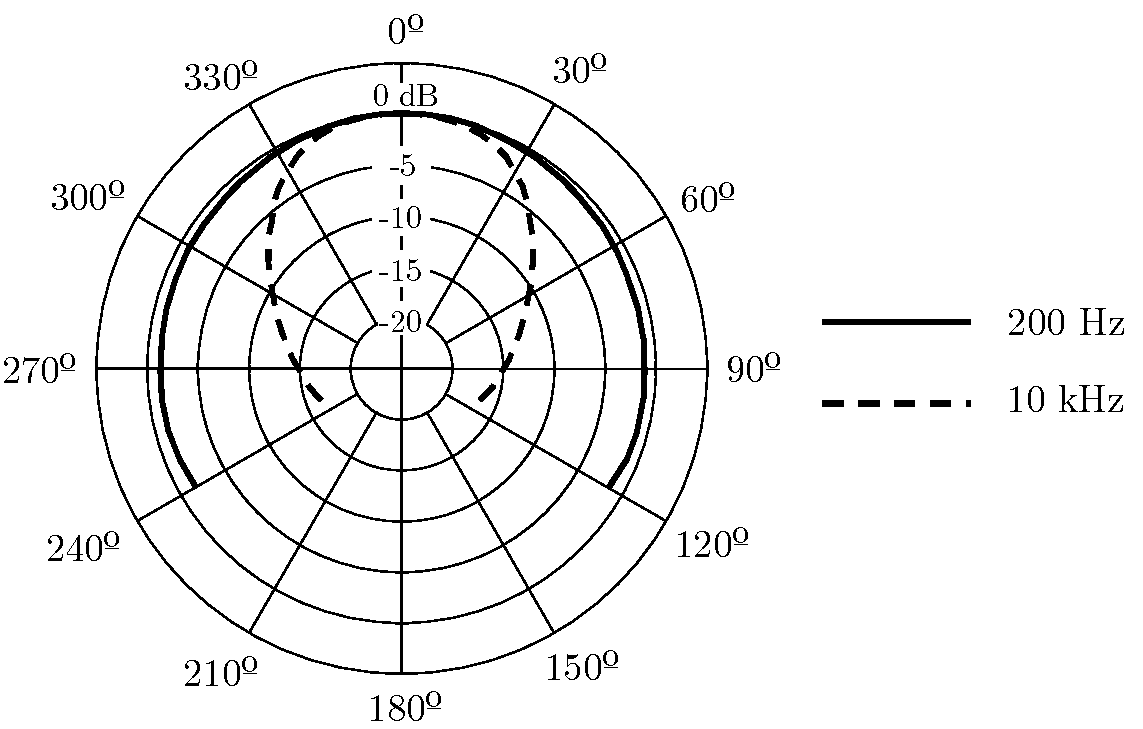
\includegraphics[width=0.6\textwidth]{archivos/diagramadirectividad.pdf}
    \caption{Diagrama de directividad de un altavoz de dos vías. Se representa la directividad emitiendo dos frecuencias diferentes.}
    \label{fig:directividad}
\end{figure}

\subsection{Factor e índice de directividad}
\label{directividad}
En ocasiones es útil tener un único valor, \textit{factor de directividad} o $Q$, que represente la directividad que tiene una fuente, sobretodo en cálculos donde se tenga en cuenta la directividad de la fuente pero no sea relevante el nivel en cada ángulo de emisión.
Este valor es la relación entre la intensidad acústica (\ref{intensidadacustica}) emitida en la dirección de máxima emisión y la que emitiría una fuente isótropa (omnidireccional) a igual potencia acústica.

\begin{flalign*}
	Q_0 = \frac{I(\theta_0,\Psi_0)}{I_{ISO}}
\end{flalign*}

La mayoría de ocasiones, la directividad no es homogénea como sí lo es en la figura \ref{fig:directividad} y para calcular un único valor hay que integrar los valores de intensidad en los diferentes ángulos de emisión:

\begin{flalign*}
	Q = \frac{4\pi I(\theta_0,\Psi_0)}{\bigintss_{\;0}^{2\pi} \bigintss_{\; 0}^{\pi} \sin (\theta) I(\theta,\Psi) \mathrm{d}\Psi \mathrm{d}\theta}
\end{flalign*}

Que teniendo en cuenta la simetría de revolución y desarrollando, el cálculo del factor de directividad se obtiene mediante:

\begin{flalign}
	Q = \frac{2}{\sum\limits_{i=1}^n \frac{I(\theta_i)}{I(\theta_0)}\sin (\theta_i) \Delta\theta_i}
\end{flalign}
\begin{condiciones}[Donde:]
	I(\theta_0) & \rightarrow & Es la intensidad en la dirección de máxima emisión.\\
	n & \rightarrow & Es el número de ángulos donde se tiene el valor de la intensidad.\\
	\Delta\theta & \rightarrow & Es la distancia en grados entre el ángulo $i$ y el ángulo $i+1$.
\end{condiciones}

En este trabajo se utilizará una fuente omnidireccional, por lo que tiene un factor de directividad $Q=1$, pero se debe tener en cuenta que esta directividad puede verse modificada por la posición de la fuente respecto al suelo, paredes o techo, tal como se muestra a continuación:

\begin{figure}[ht]
    \centering
    \begin{subfigure}[b]{0.3\textwidth}
    	\centering
        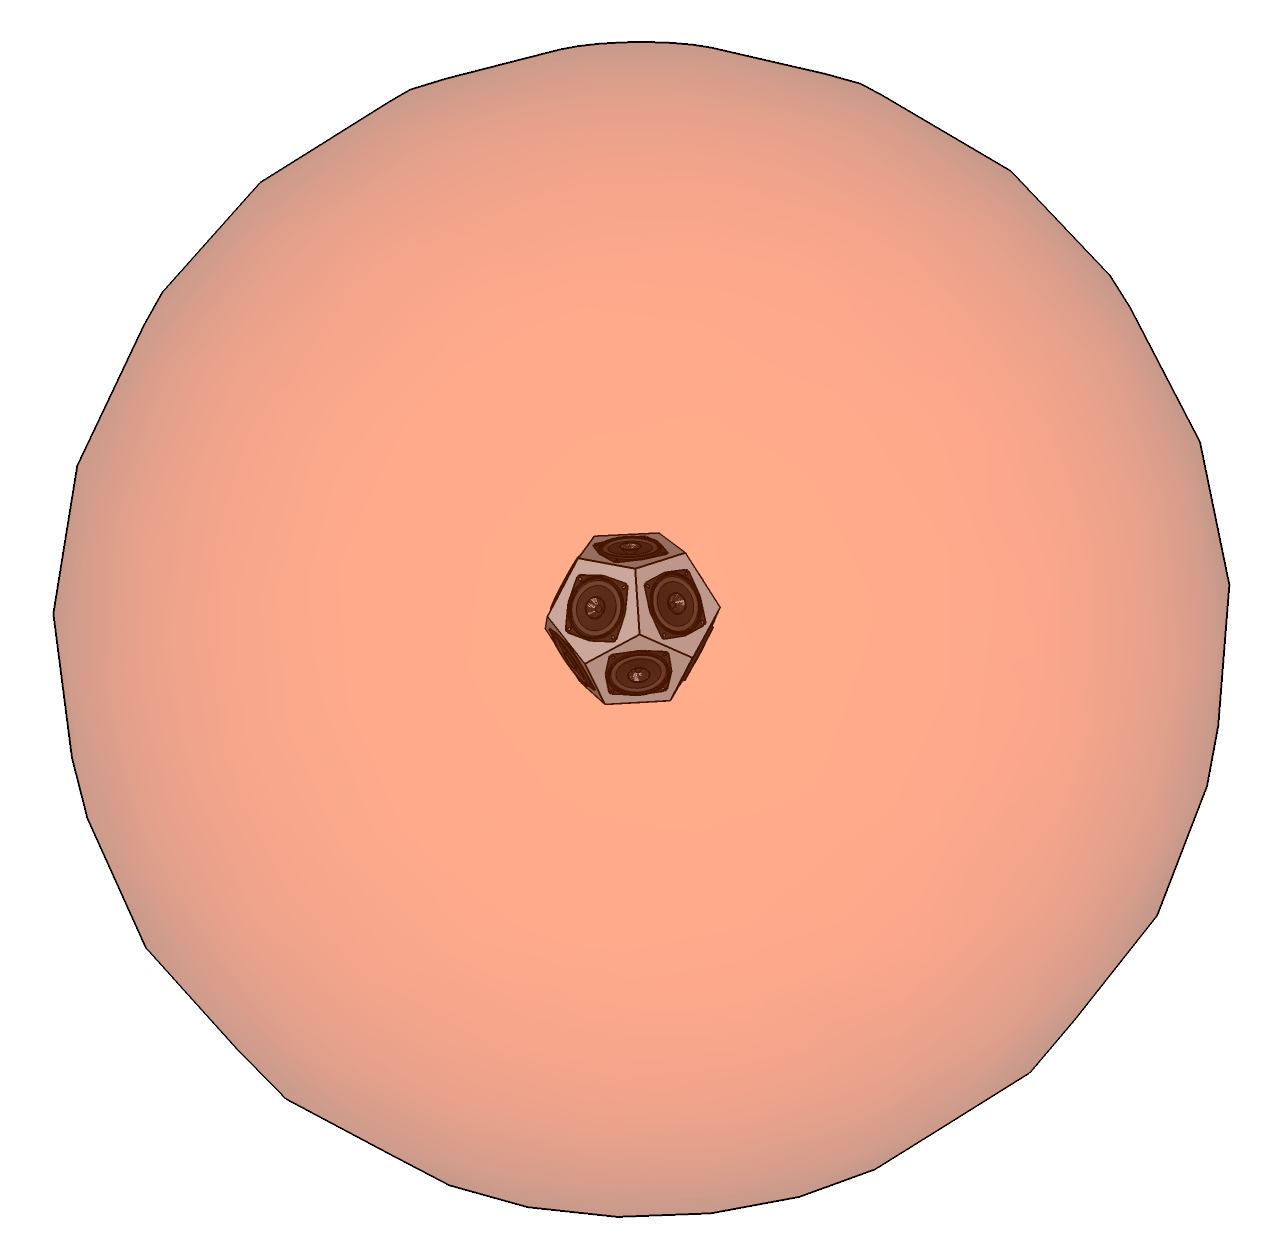
\includegraphics[width=0.5\linewidth]{archivos/Q1.png}
        \caption{$Q=1$.}
    \end{subfigure}
    ~ % Añadir el espacio deseado, si se deja la linea en blanco la siguiente subfigura ira en una nueva linea
    \begin{subfigure}[b]{0.3\textwidth}
    	\centering
        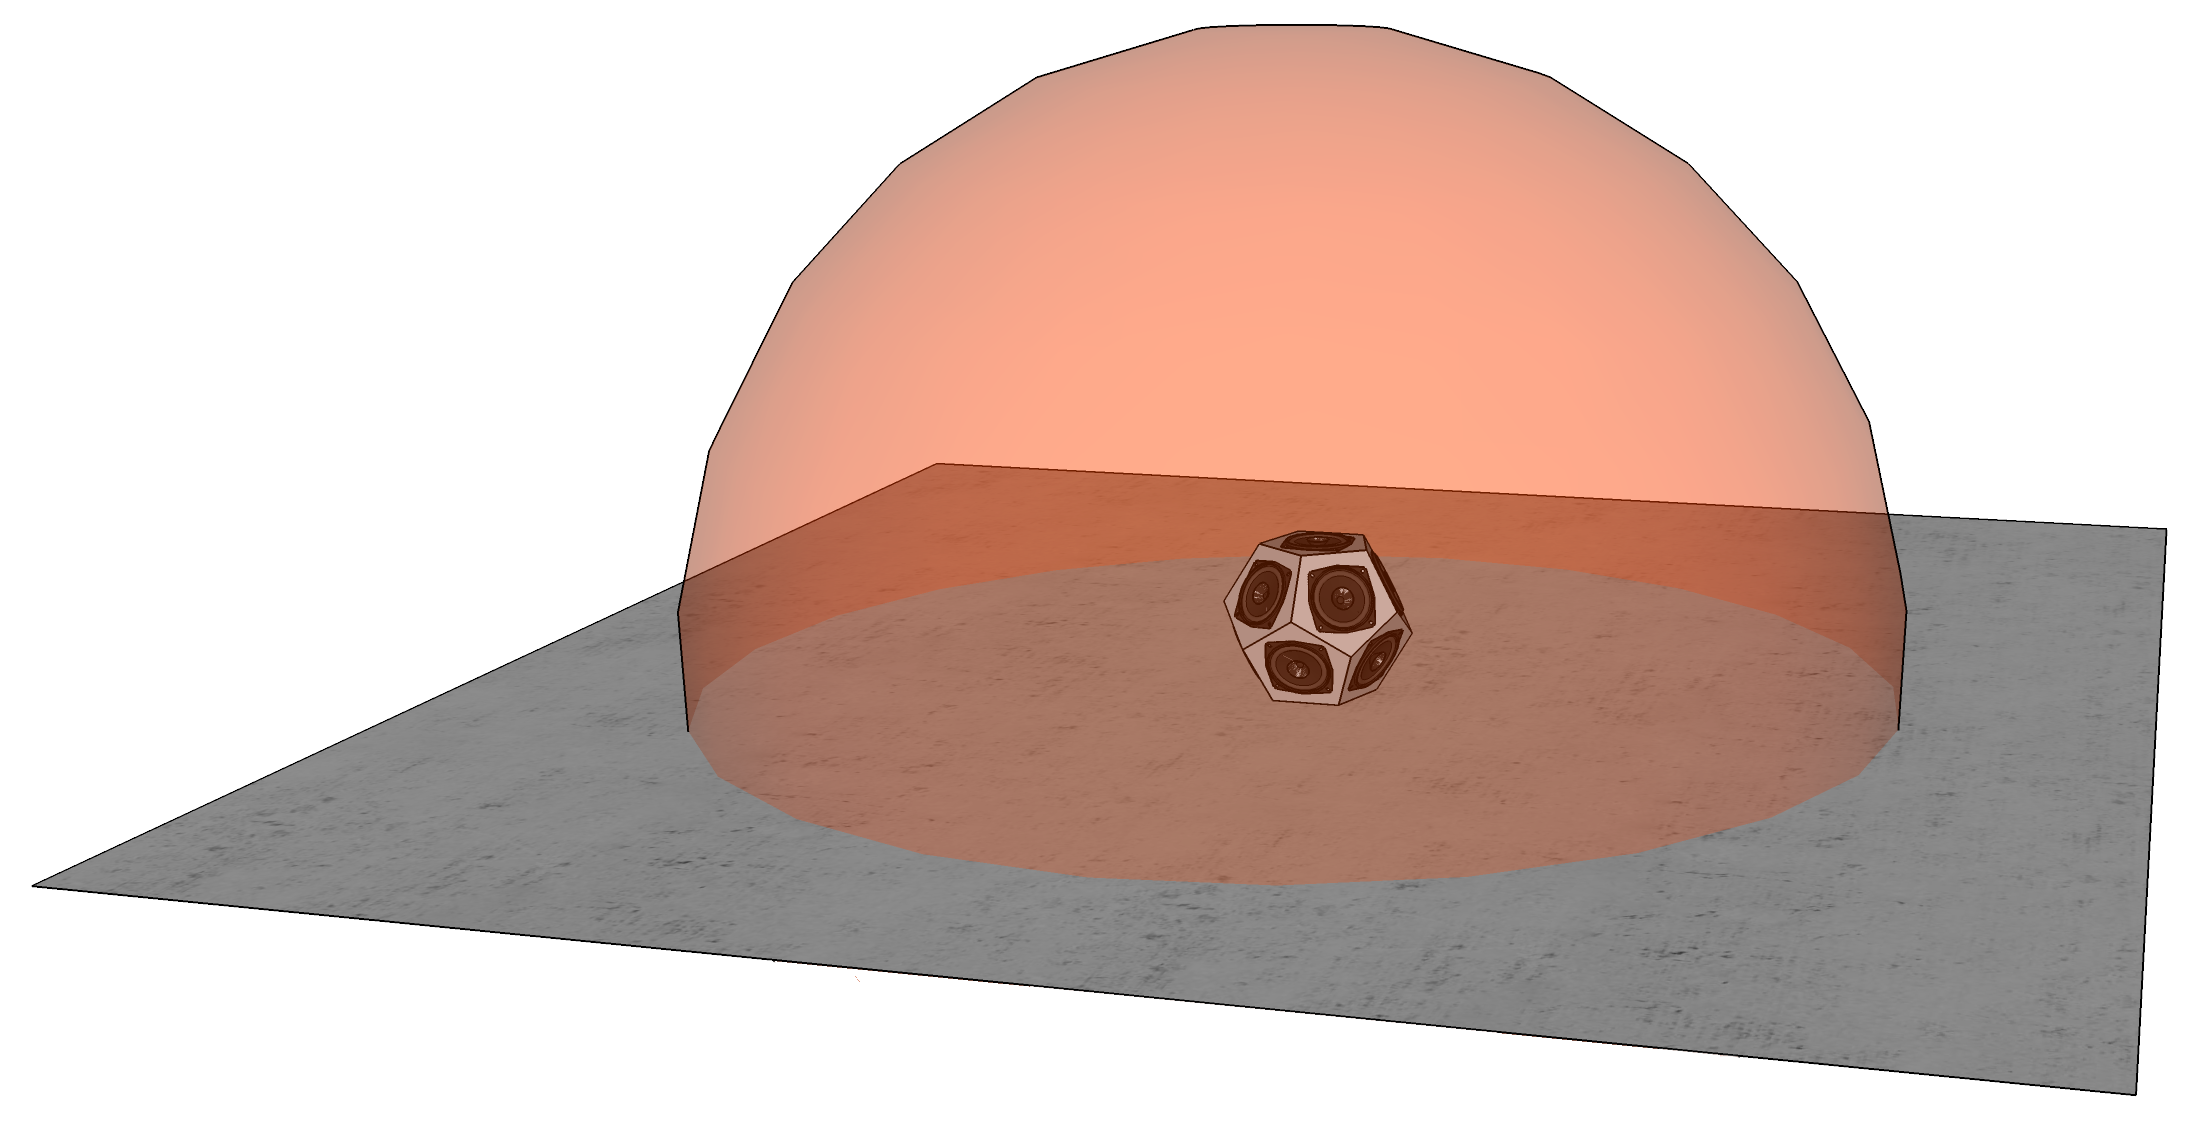
\includegraphics[width=0.8\linewidth]{archivos/Q2.png}
        \caption{$Q=2$.}
    \end{subfigure}
    
    \begin{subfigure}[b]{0.3\textwidth}
    	\centering
        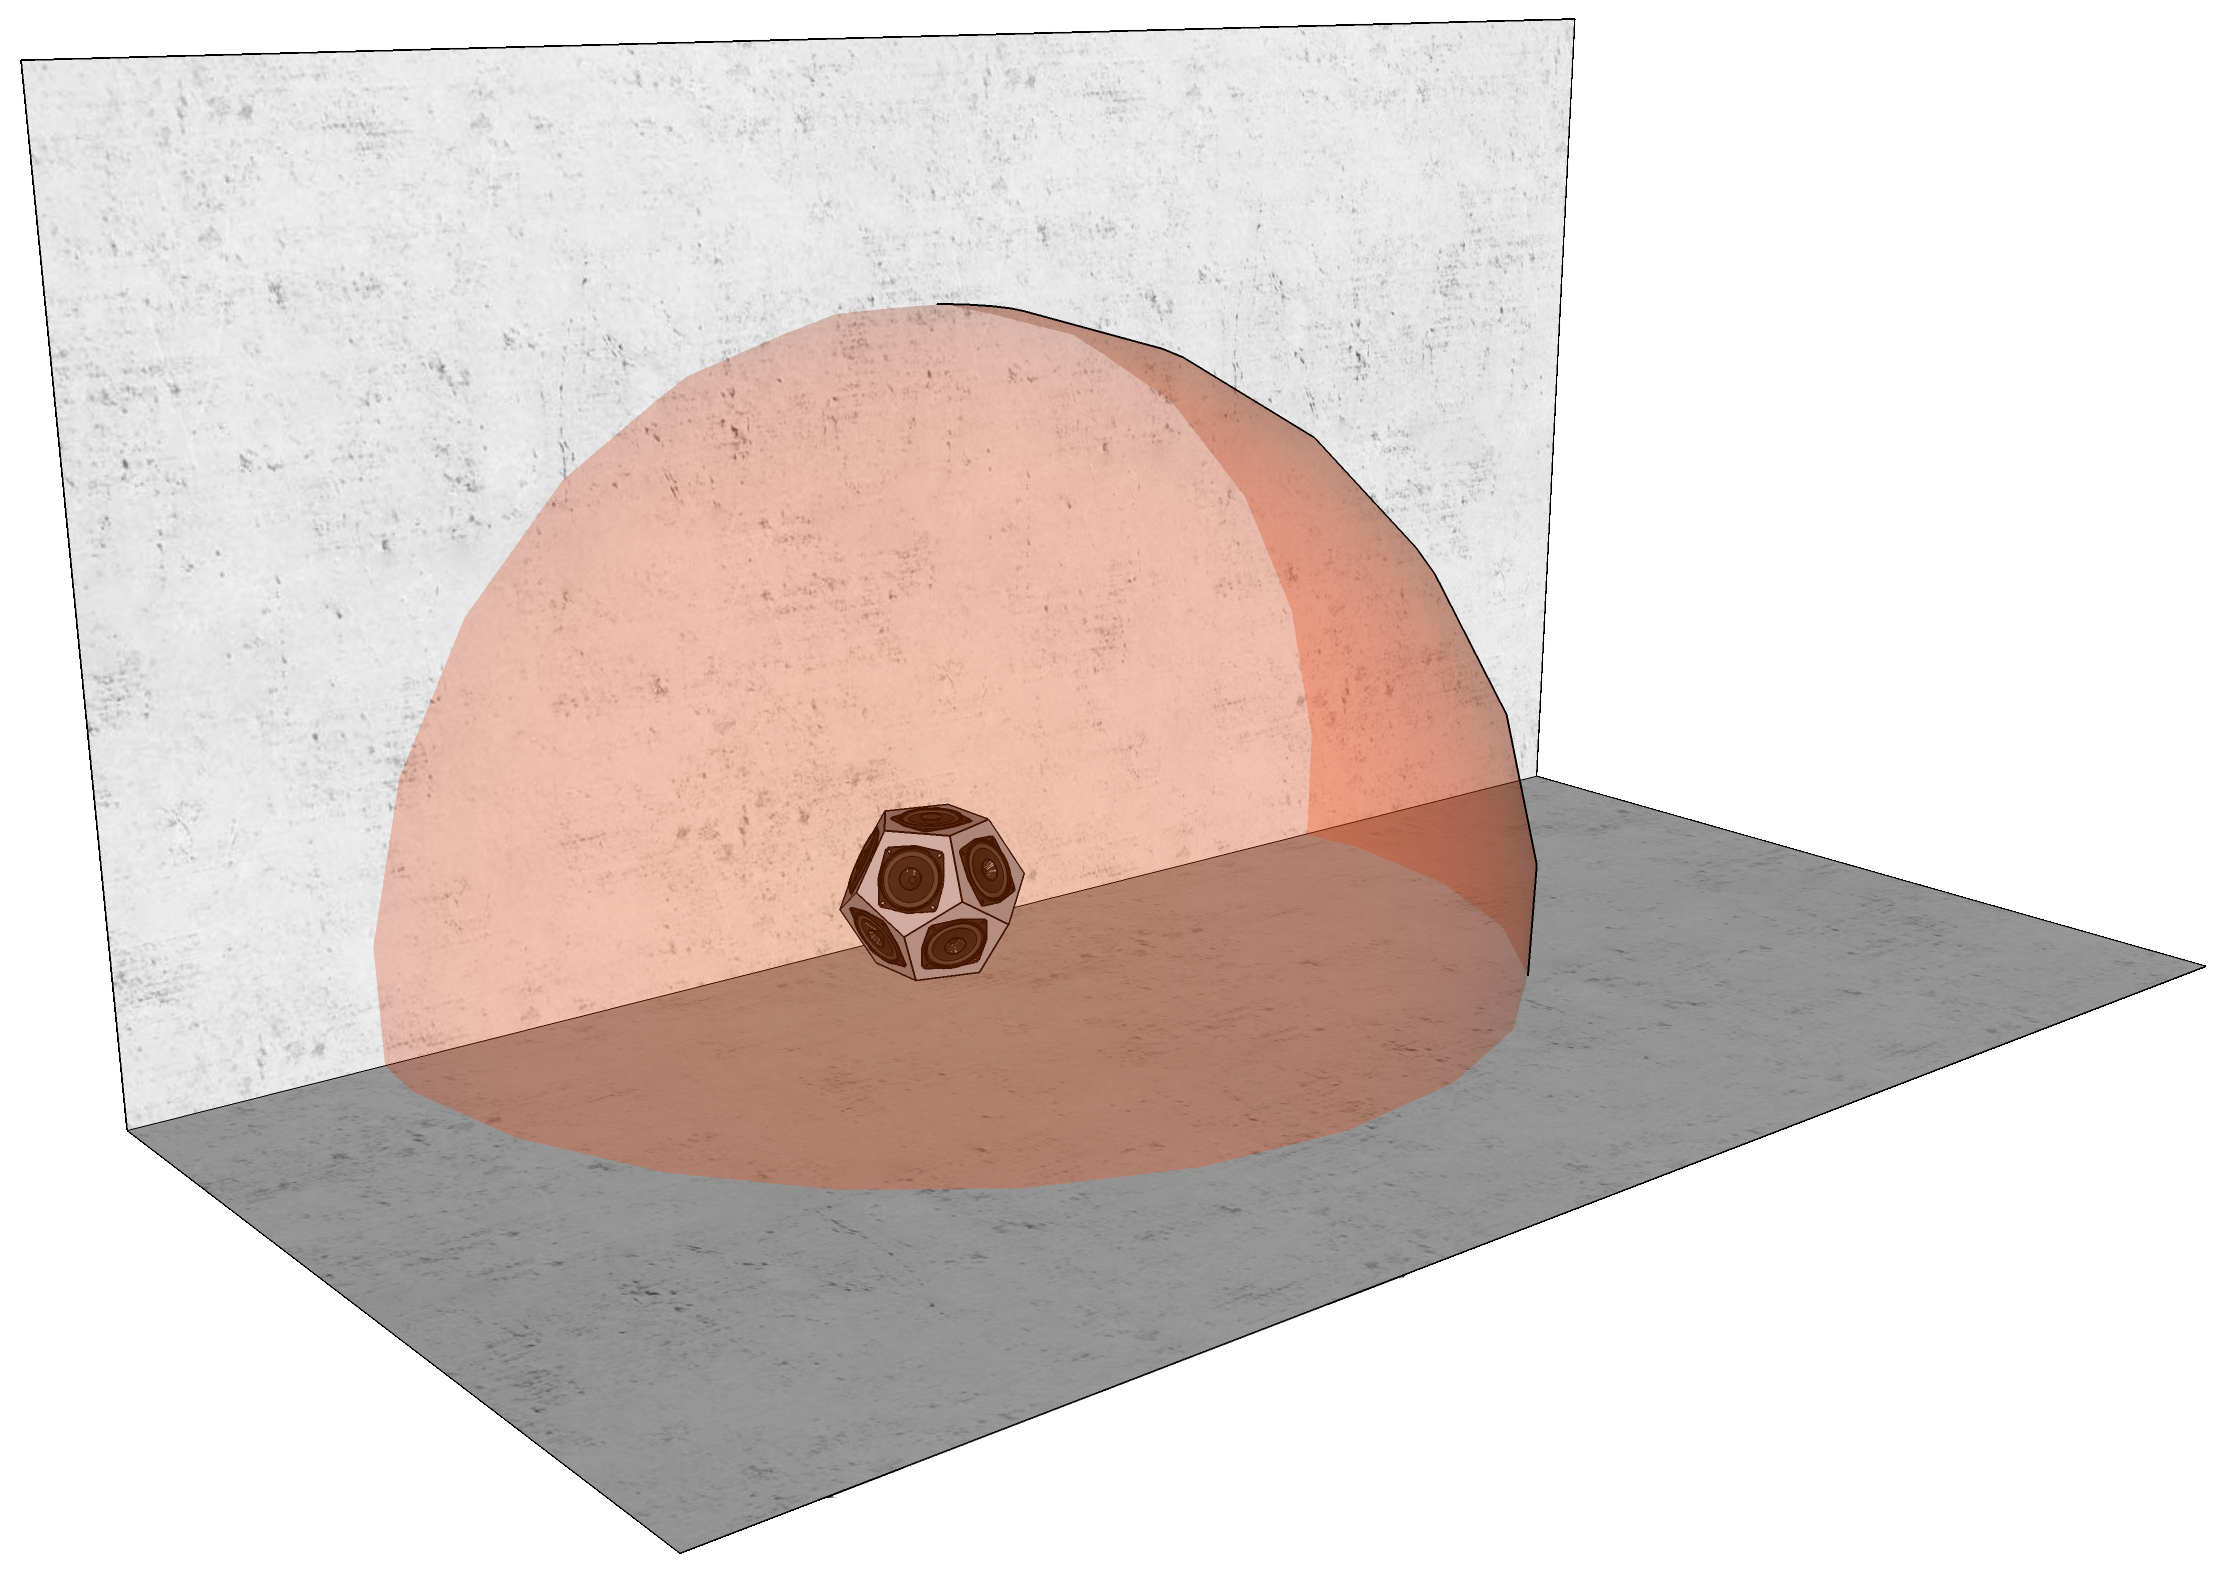
\includegraphics[width=0.8\linewidth]{archivos/Q4.png}
        \caption{$Q=4$.}
    \end{subfigure}
    ~ % Añadir el espacio deseado, si se deja la linea en blanco la siguiente subfigura ira en una nueva linea
    \begin{subfigure}[b]{0.3\textwidth}
    	\centering
        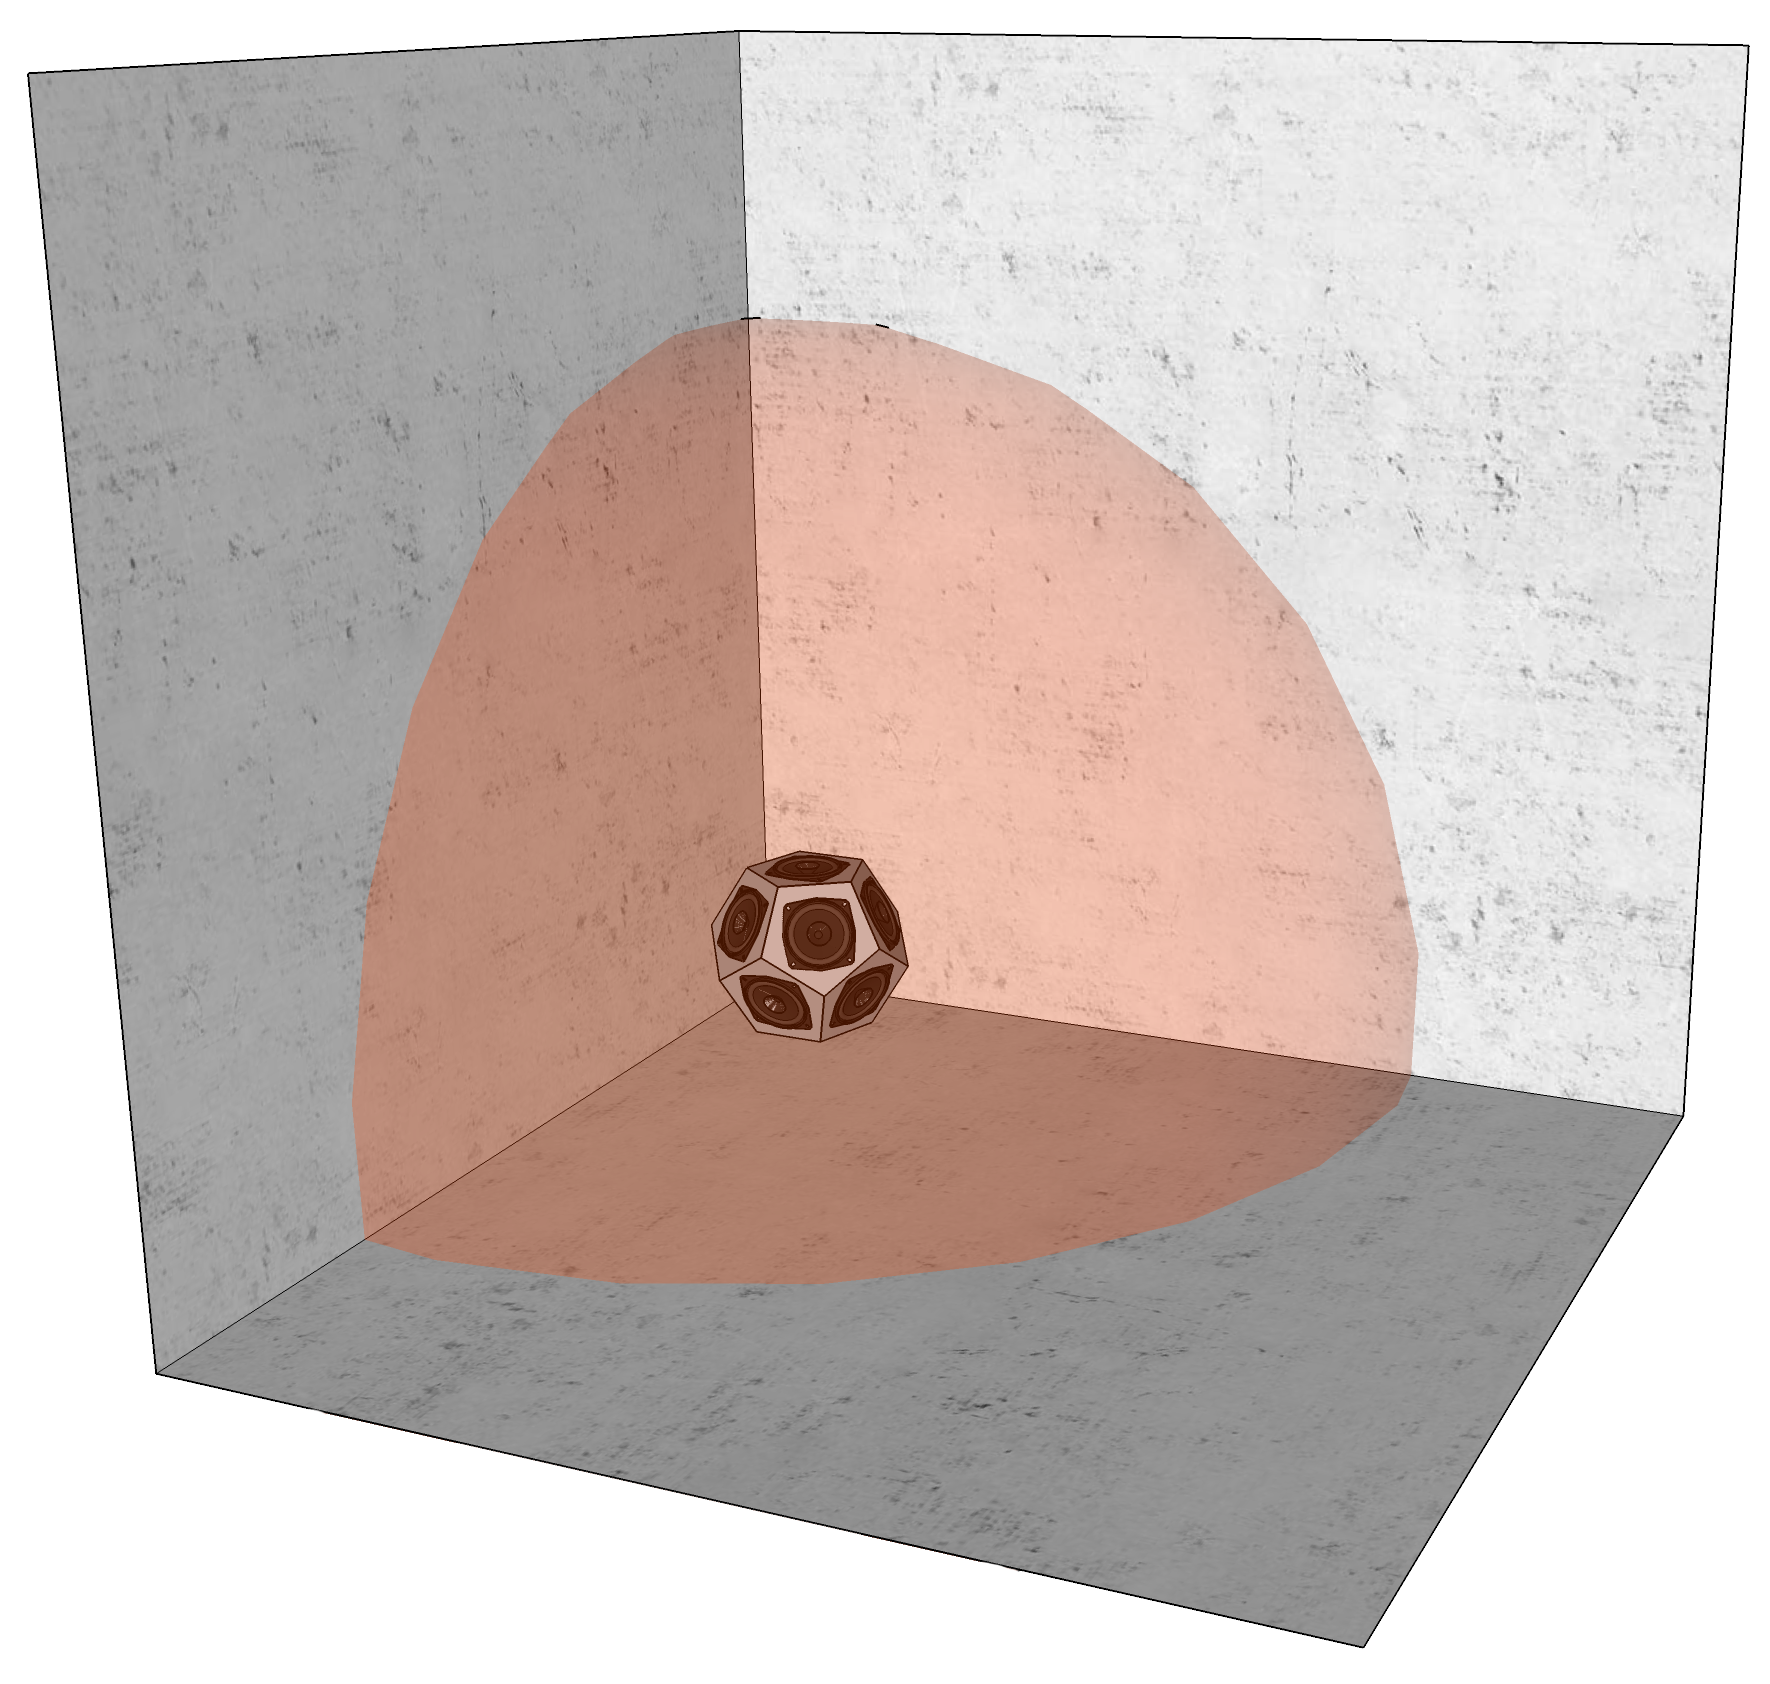
\includegraphics[width=0.6\linewidth]{archivos/Q8.png}
        \caption{$Q=8$.}
    \end{subfigure}
    \caption{Modificación del factor de directividad producido por uno o varios planos.}\label{sistemass1}
\end{figure}

El índice de directividad determina cuántos decibelios aumenta la intensidad en el eje de máxima radiación respecto a una fuente omnidireccional, se calcula:

\begin{flalign}
	DI = 10\log_{10} Q
\end{flalign}
\subsection{Potencia acústica}

La potencia acústica, representada por la letra $W$, describe la energía por unidad de tiempo que emite una fuente acústica. Es un valor intrínseco de cada fuente, es decir, no depende de las condiciones físicas del medio o la distancia, se mantiene constante.
Las unidades de este parámetro son los vatios ($W$) o los julios por segundo ($J/s$).

\subsection{Intensidad acústica}
\label{intensidadacustica}

La intensidad acústica se define como la potencia acústica por unidad de superficie, se representa con la letra $I$ y sus unidades son los $W/m^2$.

\begin{flalign}
	I = \frac{W}{S}
\end{flalign}

\subsection{Presión acústica}
Es la variación de presión local sobre la presión absoluta o atmosférica producida por las ondas acústicas, se representa con la letra $p$ y sus unidades son los pascales. La suma neta resultante es igual a la presión absoluta.

Utilizando un símil sencillo como es un muelle se pueden comprender estas variaciones locales de presión:

\begin{figure}[ht]
    \centering
    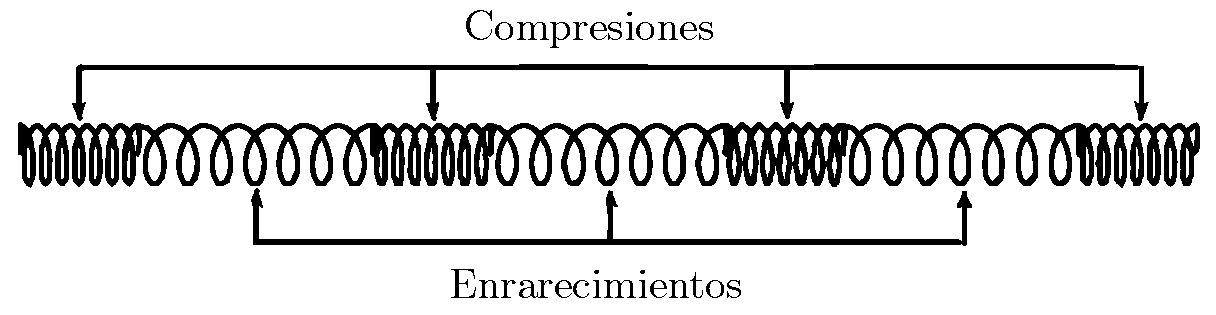
\includegraphics[width=0.6\textwidth]{archivos/presion.pdf}
    \caption{Compresión y enrarecimiento de un muelle como ejemplo de la variación de presión producida por ondas acústicas.}
\end{figure}

\subsection{Divergencia esférica}

Éste es un concepto físico necesario para comprender cómo evoluciona la intensidad acústica (\ref{intensidadacustica}) emitida por una fuente omnidireccional. La divergencia esférica describe cómo se distribuye la energía acústica emitida omnidireccionalmente en el espacio.

Una fuente acústica omnidireccional emite uniformemente intensidad en todas las direcciones, es decir, se propaga esféricamente. Según transcurre el tiempo la intensidad recorre más distancia y la esfera aumenta de tamaño distribuyendo la intensidad en una superficie aún mayor, esto se puede calcular como:

\begin{flalign}
	I = \frac{W}{S}
\end{flalign}
\begin{condiciones}[Donde:]
	W & \rightarrow & Es la potencia acústica de la fuente en vatios.\\
	I & \rightarrow & Es la intensidad recibida a una distancia $r$ en metros.\\
	S & = & $4\pi r^2$, es la superficie de una esfera de radio $r$.
\end{condiciones}


\begin{figure}[ht]
    \centering
    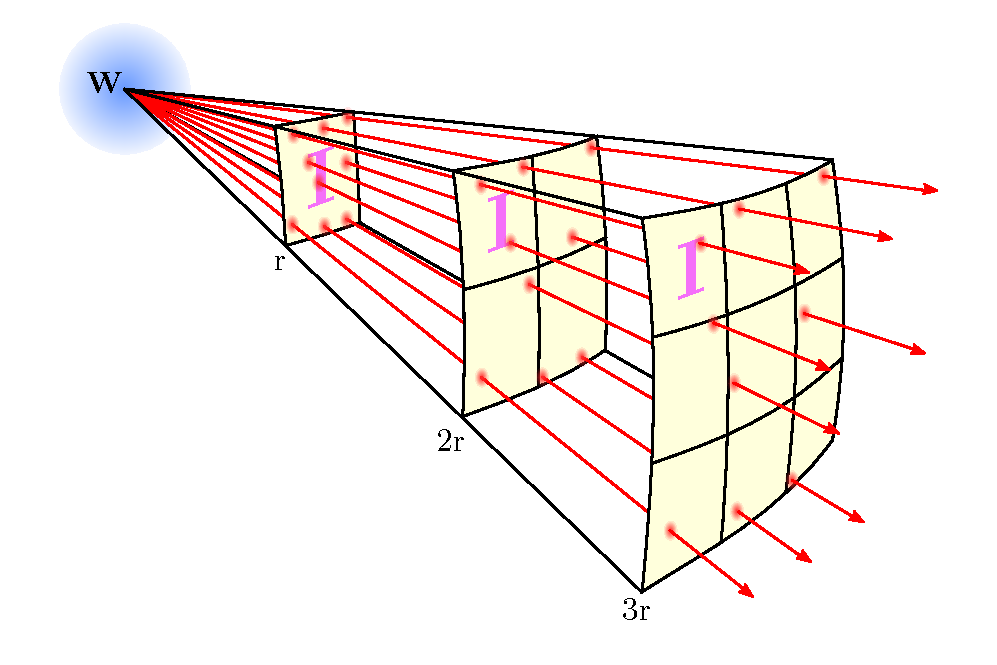
\includegraphics[width=0.6\textwidth]{archivos/divergenciaesferica.pdf}
    \caption{Representación gráfica de la divergencia esférica respecto a la distancia. Autor de la figura original: \textit{Borb}, de Wikipedia.}
\end{figure}

Si se tiene el valor de la intensidad a una distancia $r_1$ y se desea conocer el valor de intensidad a una distancia $r_2$ de la primera se puede utilizar lo que se denomina \textit{ley de la inversa del cuadrado de la distancia} que no es más que una derivación de la ecuación de la divergencia esférica.

\begin{flalign}
	I_2 = \frac{r_1^2}{r_2^2}I_1
\end{flalign}

Si la fuente tiene factor de directividad distinto a 1 (omnidireccional) se puede calcular la intensidad incluyendo el factor:

\begin{flalign}
	I = \frac{WQ}{S}
\end{flalign}
\begin{condiciones}[Donde:]
		Q & \rightarrow & Es el factor de directividad de la fuente.
\end{condiciones}

\subsection{Divergencia cilíndrica}

El concepto es el mismo que el de la divergencia esférica pero en este caso la intensidad en lugar de propagarse sobre la superficie de una esfera lo hace sobre la superficie lateral de un cilindro. Este tipo de divergencia se obtiene con fuentes lineales aunque mediante guías de ondas o alineando varias fuentes es posible modificar un frente de ondas de esférico a cilíndrico.

\begin{figure}[ht]
    \centering
    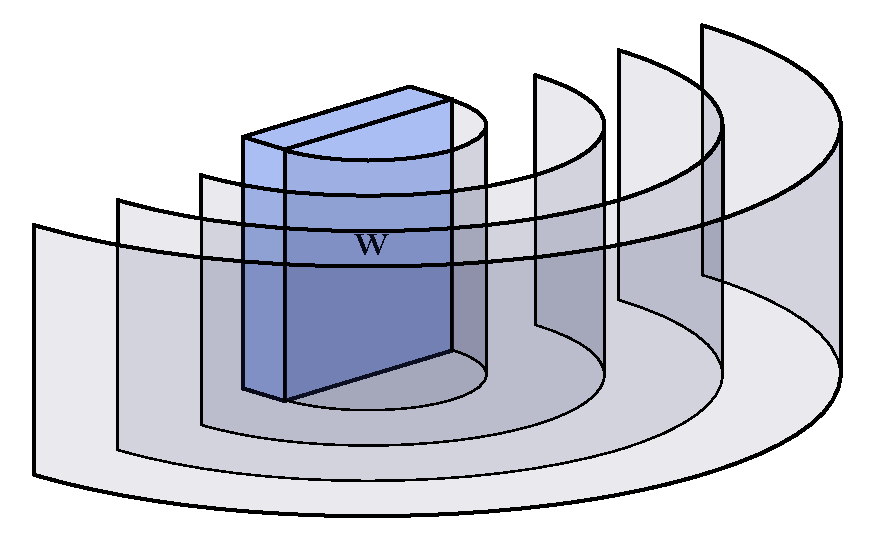
\includegraphics[width=0.6\textwidth]{archivos/divergenciacilindrica.pdf}
    \caption{Representación gráfica de la divergencia cilíndrica respecto a la distancia.}
\end{figure}
\FloatBarrier

El cálculo es el mismo que con la divergencia esférica pero teniendo en cuenta que ahora el área es el de un cilindro:

\begin{flalign}
	I = \frac{W}{S}
\end{flalign}
\begin{condiciones}[Donde:]
	S & = & $2\pi rh$, es la superficie de un cilindro de radio $r$ y altura $h$.
\end{condiciones}


\subsection{Densidad del aire}

Una densidad es la relación entre la mása y el volumen, se representa con la letra $\rho$ y sus unidades son los $Kg/m^3$. Para el caso del aire se puede calcular de forma simplificada como:

\begin{flalign}
	\rho = \frac{p}{R_{específica}T}
\end{flalign}
\begin{condiciones}[Donde:]
	p & \rightarrow & Es la presión atmosférica en pascales, 101.325 kPa.\\
	R_{específica} & \rightarrow & Es la constante específica del aire en $J\cdot(kg\cdot K)^{-1}$, para el aire seco $R_{específica}=287.058$.\\
	T & \rightarrow & Es la temperatura en kelvin. $T = 273.15 +\; ^{\circ}C$.
\end{condiciones}

\subsection{Velocidad del sonido en el aire}
La velocidad del sonido se representa con la letra $c$ y sus unidades son los $m/s$. Esta velocidad depende de la temperatura, la presión y la humedad, pero simplificando se puede calcular como:

\begin{flalign}
	c = \sqrt{\frac{\gamma RT}{M}}
\end{flalign}
\begin{condiciones}[Donde:]
	\gamma & \rightarrow & Es el coeficiente de dilatación adiabática del aire, para el aire seco $\gamma=1.4$.\\
	R & \rightarrow & Es la constante universal de los gases, $8.314\; J/(mol\cdot K)$.\\
	T & \rightarrow & Es la temperatura en kelvin. $T = 273.15 +\; ^{\circ}C$.\\
	M & \rightarrow & Es la mása molar del aire, $0.029\; kg/mol$.
\end{condiciones}

\subsection{Impedancia acústica específica del aire}

La impedancia acústica específica del aire es la oposición al flujo de energía acústica del aire, se representa con la letra $Z$ y sus unidades son $Pa\cdot s/m$ o $rayl$\footnote{La unidad $rayl$ se llama así en honor al físico John William Strutt, también conocido como Lord Rayleigh o John Rayleigh.}.

Esta impedancia se calcula mediante la densidad del aire $\rho$ y la velocidad del sonido $c$. 
\begin{flalign}
	Z = \rho c
\end{flalign}


\subsection{Escala logarítmica}

Los valores de presión, potencia o intensidad acústica sufren grandes variaciones por lo que para trabajar con ellos fácilmente se recurre a la escala logarítmica, a continuación se muestra la conversión de lineal a escala logarítmica de la presión, potencia e intensidad acústica, todos ellos son adimensionales y sus unidades son los decibelios o $dB$.

\begin{flalign}
	L_p =& 10\log_{10}\left(\frac{p_{ef}^2}{p_0^2}\right)=20\log_{10}\left(\frac{p_{ef}}{p_0}\right)\label{eq:nivelpresion} \\
	L_W =& 10\log_{10}\left(\frac{W}{W_0}\right)\\
	L_I =& 10\log_{10}\left(\frac{I}{I_0}\right)
\end{flalign}
\begin{condiciones}[Donde:]
	p_0 & \rightarrow & Es la presión de referencia, $2\cdot10^{-5}\;Pa$.\\
	W_0 & \rightarrow & Es la potencia de referencia, $1\;pW$ o $10^{-12}\;W$.\\
	I_0 & \rightarrow & Es la intensidad de referencia, $10^{-12}\;W/m^2$.
\end{condiciones}

El nivel de presión acústica $L_p$ también se suele nombrar como SPL (\textit{sound pressure level}) y el nivel de potencia como SWL.

De igual modo, si se tienen estos valores en escala logarítmica y se quiere trabajar con ellos en escala lineal, la conversión es la siguiente\footnote{Es una simple resolución matemática pero debido a múltiples errores encontrados en la literatura se ha decidido desarrollarlo.}:

\begin{flalign}
	p =& 10^{\frac{L_p}{20}}p_0\\
	W =& 10^{\frac{L_W}{10}}W_0 \\
	I =& 10^{\frac{L_I}{10}}I_0
\end{flalign}

\subsection{Relación entre presión y potencia o intensidad acústica}

Teniendo en cuenta ciertos parámetros se puede relacionar fácilmente el concepto de potencia, intensidad y presión acústica.

Si se conoce la presión acústica a una distancia $r$ de la fuente, la potencia acústica resultante será:

\begin{flalign}
	W = \frac{p_{ef}^24\pi r^2}{Z}
\end{flalign}
\begin{condiciones}[Donde:]
	p_{ef} & \rightarrow & Es la presión acústica eficaz, es la que mide cualquier sonómetro.
\end{condiciones}

Siguiendo el caso en el que se conoce la presión acústica, se puede calcular la intensidad acústica con:

\begin{flalign}\label{eq:intensidadimpedancia}
	I = \frac{p_{ef}^2}{Z}
\end{flalign}

Para los casos en los que se esté trabajando en escala logarítmica los cálculos para la potencia son:

\begin{flalign}
	L_W =& L_p + 10\log_{10}\left(\frac{4\pi r^2}{Q}\right)\\
	L_W \approx & L_p + 20\log_{10}r + 11\; ;\quad \mathrm{sí }\quad Q =1
\end{flalign}

\subsection{Bandas de frecuencia}

Las bandas de frecuencia son las fracciones en las que se divide el espectro audible (mínimo entre 20 Hz y 20000 Hz) de un sonido, se caracterizan por tener una frecuencia límite inferior $f_i$, otra superior $f_s$ y una central $f_c$. El punto de referencia para el cálculo del resto de frecuencias es la frecuencia central de 1000 Hz.

Las bandas de frecuencia en el espectro audible más habituales son la denominadas bandas de octava, entre una frecuencia central y la siguiente la relación es el doble y la relación entre sus límites y central es:
$$f_c = \sqrt{2}f_i$$
$$f_s = 2f_i$$
Otras bandas de frecuencia habituales son los tercios de octava donde las relaciones entre frecuencias centrales cumplen $2^{1/3}$, por lo que se puede observar que tres tercios dan como resultado una octava. Sus relaciones son las siguientes:
$$f_c=\sqrt[6]{2}f_i$$
$$ f_s = \sqrt[3]{2}f_i$$

\begin{table}[ht]
\centering
{\scalefont{0.9}
\begin{tabular}{@{}cccccccccc@{}}
\toprule
\multicolumn{10}{c}{Bandas de octava (Hz)}                      \\ \midrule
31.5 & 63 & 125 & 250 & 500 & 1000 & 2000 & 4000 & 8000 & 16000 \\ \bottomrule
\end{tabular}
}
\caption{Frecuencias centrales para las bandas de octava más utilizadas (ISO 266:1997).}
\end{table}

Se han desarrollado unas líneas de código Matlab para crear fácilmente cualquier fracción de bandas de frecuencia (octava: $n=1$, tercios de octava $n=3$, sextos de octava $n=6$, etc):

\begin{lstlisting}[style=Matlab-color,numbers=none, caption={Función Matlab para obtener cualquier fracción $n$ de bandas de frecuencia del espectro audible.},label=octavas]
FrecCentral = 10^3 * (2 .^ ((-6*n:4*n+n/3)/n)); % Vector de frecuencias centrales 1/n octavas
FrecDist = 2^(1/(2*n)); % Distancia entre central y corte superior o inferior
FrecSup = FrecCentral .* FrecDist; % Frecuencias límite superior
FrecInf = FrecCentral ./ FrecDist; % Frecuencias límite inferior
\end{lstlisting}


\subsection{Ponderación A}

El oído humano no percibe todas las frecuencias por igual tal como demostraron \cite{Fletcher1933}, por ello es necesario ponderar el nivel de presión de cada banda de frecuencia (octavas, tercios de octava, ...) para representar correctamente cómo lo percibirá el oído humano. La ponderación A corresponde a la inversa de la  curva de 40 fons de las curvas Fletcher-Munson.

Existen múltiples tablas en la literatura que definen el valor de corrección para cada banda de frecuencia, pero es preferible utilizar la función (obtenida mediante regresión y establecida en IEC 61672-1:2013) con la que se obtienen estos valores para cualquier frecuencia $f$:

\begin{flalign}
	A (f)= 20\log_{10}\left( \frac{12194^2f^4}{(f^2+20.6^2)\sqrt{(f^2+107.7^2)(f^2+737.9^2}\;(f^2+12194^2)} \right) + 2.0
\end{flalign}

La ponderación se aplica sumando esta al nivel de presión de la banda de frecuencia $f$.

\subsection{Suma de niveles}

En ocasiones es necesario sumar los niveles en decibelios de varias fuentes o sumar el nivel obtenido en lineal para pasarlo a bandas de octava, tercios de octava o a nivel global, para ello la suma se realiza del siguiente modo:

\begin{flalign}
	L_{sum} = 10\log_{10}\left( 10^{\nicefrac{L_1}{10}} + 10^{\nicefrac{L_2}{10}} + ... + 10^{\nicefrac{L_n}{10}}\right)
\end{flalign}
\begin{condiciones}[Donde:]
	L_1, L_2, L_n & \rightarrow & Son los n niveles en dB a sumar.
\end{condiciones}

Por ejemplo, para el paso de tercios de octava a bandas de octava la suma para obtener el valor en la banda de octava de 125 Hz será:

\begin{flalign*}
	L_{125\text{Hz}} = 10\log_{10}\left( 10^{\nicefrac{L_{100\text{Hz}}}{10}} + 10^{\nicefrac{L_{125\text{Hz}}}{10}} + 10^{\nicefrac{L_{160\text{Hz}}}{10}} \right)
\end{flalign*}

\subsection{Ruido rosa/blanco}
\label{ruidos}
En la mayoría de mediciones para conocer principalmente la respuesta en frecuencia de los elementos de emisión, captación o recintos, se emiten señales como el ruido blanco o el ruido rosa.
\\
\par
El ruido blanco se caracteriza por ser una señal con el mismo nivel en todas las frecuencias produciendo, cuando se traslada a bandas de octava, que haya un incremento de 3dB por octava dado que cada octava tiene el doble de ancho de banda que la anterior y por tanto se suma el doble de energía ($10\log_{10}(2)=3 dB$).

\begin{figure}[ht]
    \centering
    {\scalefont{0.8}
    %%%%%%%%%%%%%%%%%%%%%%%%%%%%%%%%%%%%%%%%%%%%%%%%%%%%%%%%%%%%%%%%%%%%%%%%
% Escuela Politécnica Superior de la Universidad de Alicante
% Realizado por: Jose Manuel Requena Plens
% Contacto: info@jmrplens.com / Telegram:@jmrplens
%%%%%%%%%%%%%%%%%%%%%%%%%%%%%%%%%%%%%%%%%%%%%%%%%%%%%%%%%%%%%%%%%%%%%%%%

\definecolor{mycolor1}{rgb}{0.00000,0.44700,0.74100}%
%
\begin{tikzpicture}

\begin{axis}[%
width=0.5\textwidth,
height=0.35\textwidth,
at={(0\textwidth,0\textwidth)},
scale only axis,
area style,
stack plots=y,
xmode=log,
xmin=11.5,
xmax=12000,
grid=major,
xtick={16.62,31.25,62.5,125,250,500,1000,2000,4000,8000,16000},
xticklabels={{16},{31.25},{62.5},{125},{250},{500},{1000},{2000},{4000},{8000},{16000}},
xminorticks=true,
xlabel style={font=\color{white!15!black}},
xlabel={Frecuencia (Hz)},
ymin=0,
ymax=50,
ylabel style={font=\color{white!15!black}},
ylabel={Nivel (dB)},
axis background/.style={fill=white},
legend style={at={(0.03,0.97)}, anchor=north west, legend cell align=left, align=left, draw=white!15!black}
]
\draw[line width=1.5pt,  pattern=north west lines, pattern color=orange] (axis cs:12.0485434560398,-10) rectangle (axis cs:22.0970869120796,20.7918124604762);
\draw[line width=1.5pt,  pattern=north west lines, pattern color=orange] (axis cs:22.0970869120796,-10) rectangle (axis cs:44.1941738241592,23.6172783601759);
\draw[line width=1.5pt,  pattern=north west lines, pattern color=orange] (axis cs:44.1941738241592,-10) rectangle (axis cs:88.3883476483184,26.5321251377534);
\draw[line width=1.5pt, pattern=north west lines, pattern color=orange] (axis cs:88.3883476483184,-10) rectangle (axis cs:176.776695296637,29.4939000664491);
\draw[line width=1.5pt,  pattern=north west lines, pattern color=orange] (axis cs:176.776695296637,-10) rectangle (axis cs:353.553390593274,32.5042000230889);
\draw[line width=1.5pt,  pattern=north west lines, pattern color=orange] (axis cs:353.553390593274,-10) rectangle (axis cs:707.106781186548,35.5022835305509);
\draw[line width=1.5pt,  pattern=north west lines, pattern color=orange] (axis cs:707.106781186547,-10) rectangle (axis cs:1414.2135623731,38.5003325768977);
\draw[line width=1.5pt,  pattern=north west lines, pattern color=orange] (axis cs:1414.21356237309,-10) rectangle (axis cs:2828.42712474619,41.5075643986031);
\draw[line width=1.5pt,  pattern=north west lines, pattern color=orange] (axis cs:2828.42712474619,-10) rectangle (axis cs:5656.85424949238,44.5163294745699);
\draw[line width=1.5pt,  pattern=north west lines, pattern color=orange] (axis cs:5656.85424949238,-10) rectangle (axis cs:11313.7084989848,47.5266294312097);
\addlegendimage{line width=1.5pt,  pattern=north west lines, pattern color=orange}
\addlegendentry{Ruido blanco - octavas}

\addplot[fill=mycolor1, draw=black] table[row sep=crcr]{%
1	20\\
16000	20\\
}
\closedcycle;
\addlegendentry{Ruido blanco - lineal}

\end{axis}
\end{tikzpicture}%
    }
    \caption{Representación de ruido blanco tanto en lineal como por octavas.}
    \label{graf:ruidoblanco}
\end{figure}
\FloatBarrier
El ruido rosa corrige el efecto producido en el ruido blanco, introduciendo una atenuación de 3dB por octava, es por ello por lo que es el ruido más habitual en mediciones que se analizan por bandas de octava, ya que mantiene el mismo valor de energía en todas las bandas de octava.

\begin{figure}[ht]
    \centering
    {\scalefont{0.8}
    %%%%%%%%%%%%%%%%%%%%%%%%%%%%%%%%%%%%%%%%%%%%%%%%%%%%%%%%%%%%%%%%%%%%%%%%
% Plantilla TFG/TFM
% Escuela Politécnica Superior de la Universidad de Alicante
% Realizado por: Jose Manuel Requena Plens
% Contacto: info@jmrplens.com / Telegram:@jmrplens
%%%%%%%%%%%%%%%%%%%%%%%%%%%%%%%%%%%%%%%%%%%%%%%%%%%%%%%%%%%%%%%%%%%%%%%%

\definecolor{mycolor1}{rgb}{0.00000,0.44700,0.74100}%
%
\begin{tikzpicture}

\begin{axis}[%
width=0.5\textwidth,
height=0.35\textwidth,
at={(0\textwidth,0\textwidth)},
scale only axis,
area style,
stack plots=y,
xmode=log,
xmin=11.5,
xmax=12000,
grid=major,
xtick={16.62,31.25,62.5,125,250,500,1000,2000,4000,8000,16000},
xticklabels={{16},{31.25},{62.5},{125},{250},{500},{1000},{2000},{4000},{8000},{16000}},
xminorticks=true,
xlabel style={font=\color{white!15!black}},
xlabel={Frecuencia (Hz)},
ymin=0,
ymax=50,
ylabel style={font=\color{white!15!black}},
ylabel={Nivel (dB)},
axis background/.style={fill=white},
legend style={at={(0.03,0.97)}, anchor=north west, legend cell align=left, align=left, draw=white!15!black}
]
\draw[line width=1.5pt,  pattern=north west lines, pattern color=orange] (axis cs:12.0485434560398,-10) rectangle (axis cs:22.0970869120796,38.5395005764647);
\draw[line width=1.5pt,  pattern=north west lines, pattern color=orange] (axis cs:22.0970869120796,-10) rectangle (axis cs:44.1941738241592,38.4765584900126);
\draw[line width=1.5pt,  pattern=north west lines, pattern color=orange] (axis cs:44.1941738241592,-10) rectangle (axis cs:88.3883476483184,38.4431162668429);
\draw[line width=1.5pt,  pattern=north west lines, pattern color=orange] (axis cs:88.3883476483184,-10) rectangle (axis cs:176.776695296637,38.4258681272424);
\draw[line width=1.5pt,  pattern=north west lines, pattern color=orange] (axis cs:176.776695296637,-10) rectangle (axis cs:353.553390593274,38.4347351341331);
\draw[line width=1.5pt,  pattern=north west lines, pattern color=orange] (axis cs:353.553390593274,-10) rectangle (axis cs:707.106781186548,38.4215119396158);
\draw[line width=1.5pt,  pattern=north west lines, pattern color=orange] (axis cs:707.106781186547,-10) rectangle (axis cs:1414.2135623731,38.4104672378742);
\draw[line width=1.5pt,  pattern=north west lines, pattern color=orange] (axis cs:1414.21356237309,-10) rectangle (axis cs:2828.42712474619,38.4093616516654);
\draw[line width=1.5pt,  pattern=north west lines, pattern color=orange] (axis cs:2828.42712474619,-10) rectangle (axis cs:5656.85424949238,38.4088083131028);
\draw[line width=1.5pt,  pattern=north west lines, pattern color=orange] (axis cs:5656.85424949238,-10) rectangle (axis cs:11313.7084989848,38.4090852235989);
\addlegendimage{line width=1.5pt,  pattern=north west lines, pattern color=orange}
\addlegendentry{Ruido rosa - octavas}

\addplot[fill=mycolor1, draw=black] table[row sep=crcr]{%
1	50\\
16000	7.95880017344075\\
}
\closedcycle;
\addlegendentry{Ruido rosa - lineal}

\end{axis}
\end{tikzpicture}%
    }
    \caption{Representación de ruido rosa tanto en lineal como por octavas.}
    \label{graf:ruidorosa}
\end{figure}
\FloatBarrier


\subsection{Nivel continuo equivalente}

El nivel continuo equivalente es la media energética del nivel de un ruido o sonido promediado en el tiempo, es básicamente un nivel promedio de una medida contínua. Debido a la alta variabilidad de nivel de un sonido no es correcto escoger un valor de un instante concreto, se debe obtener un promedio de todos los valores instantáneos obtenidos. 

Este nivel se puede calcular como:

\begin{flalign}
	L_{eq} = 10\log_{10}\left( \frac{1}{T} \bigintsss_0^{T}\left( \frac{p^2(t)}{p^2_0} \right)\text{d}t \right)
\end{flalign}
\begin{condiciones}[Donde:]
	p^2(t) & \rightarrow & Son los valores instantáneos de presión al cuadrado.\\
	T & \rightarrow & Es la duración de la medida.
\end{condiciones}

Para entenderlo fácilmente se muestra en la figura \ref{graf:leq} una señal captada y su valor $L_{eq}$.

\begin{figure}[ht]
    \centering
    {\scalefont{0.8}
    %%%%%%%%%%%%%%%%%%%%%%%%%%%%%%%%%%%%%%%%%%%%%%%%%%%%%%%%%%%%%%%%%%%%%%%%
% Escuela Politécnica Superior de la Universidad de Alicante
% Realizado por: Jose Manuel Requena Plens
% Contacto: info@jmrplens.com / Telegram:@jmrplens
%%%%%%%%%%%%%%%%%%%%%%%%%%%%%%%%%%%%%%%%%%%%%%%%%%%%%%%%%%%%%%%%%%%%%%%%

\definecolor{mycolor1}{rgb}{0.00000,0.44700,0.74100}%
\definecolor{mycolor2}{rgb}{0.85000,0.32500,0.09800}%
%
\begin{tikzpicture}

\begin{axis}[%
width=0.5\textwidth,
height=0.22\textwidth,
at={(0\textwidth,0\textwidth)},
scale only axis,
xmin=0,
xmax=1,
xlabel style={font=\color{white!15!black}},
xlabel={Tiempo (s)},
ymin=44,
ymax=58,
ylabel style={font=\color{white!15!black}},
ylabel={Nivel (dB)},
axis background/.style={fill=white},
legend style={legend cell align=left, align=left, draw=white!15!black}
]
\addplot [color=mycolor1, line width=1.5pt]
  table[row sep=crcr]{%
0	50\\
0.00598412698412432	52.4354905344046\\
0.00923265306122545	53.5863011944272\\
0.0117972789115655	54.3566439459881\\
0.0140199546485249	54.9087296789833\\
0.0160716553288012	55.3167194619479\\
0.0177814058956898	55.5811991715484\\
0.0193201814058952	55.761725842872\\
0.0206879818594103	55.8783677034787\\
0.0218848072562352	55.94850013745\\
0.0229106575963698	55.9864430085202\\
0.0237655328798212	56.0035077107261\\
0.0242784580498849	56.0077962188932\\
0.0246204081632655	56.0083021094971\\
0.0249623582766461	56.006998772416\\
0.0254752834467098	56.0017924852514\\
0.0261591836734709	55.9891287470019\\
0.0270140589569152	55.964866713046\\
0.0282108843537401	55.917113228018\\
0.0297496598639455	55.8365743707716\\
0.031972335600905	55.6946034737216\\
0.0382984126984098	55.2754066432793\\
0.0401791383219958	55.1830307099835\\
0.0417179138322012	55.1265260868083\\
0.0429147392290261	55.0956856199849\\
0.0439405895691607	55.0787261109273\\
0.044795464852605	55.0713075112947\\
0.0453083900226758	55.0697543991762\\
0.0456503401360564	55.0699075357098\\
0.0459922902494299	55.0709970048091\\
0.0465052154195007	55.0743537532379\\
0.0471891156462618	55.0819503877214\\
0.0480439909297061	55.0962202298286\\
0.049240816326531	55.1243828267478\\
0.0507795918367364	55.172654131706\\
0.0528312925170056	55.2526687159606\\
0.059499319727891	55.5270521762376\\
0.0610380952380964	55.5691566346894\\
0.0622349206349213	55.5912047631082\\
0.0630897959183656	55.6003790190219\\
0.0636027210884365	55.6030481201545\\
0.063944671201817	55.6035964552583\\
0.0642866213151905	55.6031352708759\\
0.0647995464852613	55.6005094439748\\
0.0654834467120153	55.5933129193599\\
0.0663383219954667	55.5782339045611\\
0.0673641723356013	55.5510446711095\\
0.0685609977324262	55.5066901016045\\
0.0699287981859413	55.4395422431632\\
0.071638548752837	55.3320164838049\\
0.0736902494331062	55.1717762067451\\
0.0762548752834462	54.9330280877809\\
0.0803582766439916	54.5022082506331\\
0.0846326530612274	54.0657081040926\\
0.0871972789115674	53.8463091484114\\
0.0892489795918365	53.7068243121441\\
0.0909587301587322	53.6193736597434\\
0.0923265306122474	53.5695720913139\\
0.0935233560090722	53.540957576204\\
0.0943782312925165	53.5289806251965\\
0.0950621315192777	53.5243535395645\\
0.0954040816326511	53.5236495705989\\
0.0957460317460317	53.523993553022\\
0.0960879818594123	53.5253639467535\\
0.096600907029476	53.5292916732686\\
0.0972848072562371	53.5378824132796\\
0.0983106575963717	53.5574570349797\\
0.0995074829931966	53.589293956492\\
0.101217233560092	53.6482056726565\\
0.103952834467123	53.7613545296413\\
0.107030385487526	53.8852252003745\\
0.108569160997732	53.9329238430555\\
0.109765986394557	53.9587877425379\\
0.110620861678008	53.9697707860655\\
0.111133786848072	53.9729655370425\\
0.111475736961452	53.9735754401465\\
0.111646712018143	53.9734061680292\\
0.111988662131516	53.9720897026781\\
0.112501587301587	53.9675847530432\\
0.113185487528348	53.9566267982607\\
0.114040362811792	53.9345181675708\\
0.115066213151927	53.894909844778\\
0.116263038548752	53.8296391955825\\
0.117630839002267	53.7287143078679\\
0.119169614512472	53.58056254502\\
0.120879365079368	53.3726807435709\\
0.122931065759637	53.0648349692087\\
0.125324716553287	52.63195704156\\
0.128231292517007	52.0188965665263\\
0.132676643990926	50.9728098492146\\
0.137976870748297	49.7464071698251\\
0.140883446712017	49.1734960804138\\
0.143106122448977	48.8130669029894\\
0.144986848072563	48.5704555848487\\
0.146696598639458	48.4035903571865\\
0.148064399092974	48.3080352645967\\
0.149261224489798	48.2520817101192\\
0.150116099773243	48.2276446720638\\
0.150799999999997	48.2171783741505\\
0.151312925170068	48.2144898852167\\
0.151654875283448	48.2150973258981\\
0.151996825396829	48.2175842741123\\
0.152509750566892	48.2247561656879\\
0.153193650793654	48.2405265016715\\
0.154219501133788	48.276742309395\\
0.155416326530613	48.3363917765509\\
0.156955102040818	48.4367998851375\\
0.159006802721088	48.6026366734534\\
0.162597278911562	48.937167690639\\
0.166016780045354	49.2404358226117\\
0.168068480725623	49.3849724235891\\
0.169607256235828	49.4649640458562\\
0.170804081632653	49.5070335294376\\
0.171658956916097	49.5252080414222\\
0.172342857142858	49.5322221102209\\
0.172684807256239	49.5331452722564\\
0.172855782312922	49.5329506885399\\
0.173197732426303	49.5312365786132\\
0.173710657596374	49.5253204908182\\
0.174394557823128	49.5111159593275\\
0.175249433106579	49.483109792913\\
0.176275283446714	49.4344202386435\\
0.177472108843538	49.3570110485449\\
0.179010884353744	49.2258792677841\\
0.180720634920633	49.0411581327237\\
0.182772335600909	48.7717738247189\\
0.185507936507939	48.3497047093896\\
0.190808163265309	47.4425225114763\\
0.194398639455784	46.8703030568826\\
0.196792290249434	46.553012272762\\
0.198673015873013	46.3541771017598\\
0.200211791383218	46.2297650090181\\
0.201579591836733	46.1503653509219\\
0.202605442176868	46.1107947731683\\
0.203460317460319	46.0910865112234\\
0.204144217687073	46.0840136411358\\
0.204486167800454	46.0833620008552\\
0.204828117913834	46.0846215078295\\
0.205341043083898	46.0900666070504\\
0.206024943310659	46.1038797536169\\
0.206879818594103	46.1314475355647\\
0.207905668934238	46.1791034408031\\
0.209273469387753	46.2659383951959\\
0.210812244897959	46.3925325489547\\
0.212863945578235	46.6016710673063\\
0.215428571428575	46.911107262663\\
0.225174149659864	48.1372865059723\\
0.227396825396823	48.3405936566567\\
0.229277551020409	48.4737618879328\\
0.230816326530615	48.5543515252333\\
0.23218412698413	48.60426633714\\
0.233209977324265	48.628518418714\\
0.234064852607709	48.6403827773358\\
0.23474875283447	48.6446246087346\\
0.235090702947844	48.6450587597203\\
0.235432653061224	48.6444028888133\\
0.235945578231295	48.6414369874469\\
0.236629478458049	48.6339422118275\\
0.237484353741493	48.6192557587475\\
0.238681179138325	48.5897827623002\\
0.240219954648524	48.5391188802128\\
0.2422716553288	48.4555773599565\\
0.249110657596368	48.1639985848597\\
0.250820408163264	48.1143188720163\\
0.252188208616779	48.0867152592828\\
0.253214058956914	48.0738836076406\\
0.253897959183675	48.0692604497106\\
0.254410884353739	48.0678971397999\\
0.254752834467119	48.067996395486\\
0.2550947845805	48.0689027747083\\
0.255607709750564	48.0717713382109\\
0.256291609977325	48.0783878528064\\
0.257146485260769	48.0910522002761\\
0.258343310657594	48.1166212829081\\
0.259711111111109	48.1561087345516\\
0.261420861678005	48.2184907175902\\
0.263985487528345	48.3306474956782\\
0.268943764172334	48.550836306189\\
0.27065351473923	48.6076300071772\\
0.272021315192745	48.6396405856957\\
0.27304716553288	48.6541251199986\\
0.273731065759634	48.6587063064382\\
0.274073015873014	48.6593772998538\\
0.274414965986395	48.6589292347146\\
0.274756916099776	48.6573347981512\\
0.275269841269839	48.6527384572647\\
0.2759537414966	48.6423758233884\\
0.276808616780045	48.6224026004332\\
0.277834467120179	48.5878426441998\\
0.279031292517004	48.532637077406\\
0.280399092970519	48.449880211023\\
0.282108843537415	48.3177497797406\\
0.284160544217684	48.1204170021778\\
0.286554195011341	47.845756358698\\
0.290315646258506	47.3559476209446\\
0.294760997732425	46.7877753004496\\
0.296983673469384	46.5541775598426\\
0.29869342403628	46.4142106774319\\
0.300061224489795	46.3332106651333\\
0.30108707482993	46.2929933244866\\
0.301941950113381	46.2740503553424\\
0.302454875283445	46.2693635437881\\
0.302625850340135	46.2689454472509\\
0.302796825396825	46.269107405271\\
0.303138775510206	46.2711894840592\\
0.30365170068027	46.2787711880909\\
0.304335600907031	46.2973620151626\\
0.305190476190475	46.334518530219\\
0.30621632653061	46.399910819006\\
0.307413151927435	46.5052549663249\\
0.30878095238095	46.664004062702\\
0.310490702947845	46.9189221564951\\
0.312371428571431	47.2683060542021\\
0.314594104308391	47.765356423519\\
0.317329705215421	48.4799196121116\\
0.321262131519276	49.6330463354924\\
0.327588208616781	51.4894805069492\\
0.330494784580502	52.212945761074\\
0.332717460317461	52.6703694875504\\
0.33459818594104	52.9804377590511\\
0.336307936507936	53.1957378105521\\
0.337675736961451	53.3205845693593\\
0.338872562358276	53.3949431139119\\
0.33989841269841	53.4329745181215\\
0.340582312925171	53.4453678042553\\
0.341095238095235	53.4479887278421\\
0.341266213151926	53.4476097420882\\
0.341608163265306	53.4449963716615\\
0.342121088435377	53.4365023546497\\
0.342804988662131	53.4168367832443\\
0.343659863945575	53.3793242941407\\
0.344856689342407	53.3040047470422\\
0.346224489795915	53.1880553022591\\
0.347934240362811	53.0040291488192\\
0.35015691609977	52.7129336136982\\
0.353405442176872	52.2207523753449\\
0.359902494331067	51.2247111677433\\
0.362467120181407	50.8992691556285\\
0.364689795918366	50.6688076687589\\
0.366570521541952	50.5153171133509\\
0.368280272108841	50.409439713517\\
0.369819047619046	50.3406767895916\\
0.371015873015871	50.3034653677367\\
0.372041723356013	50.2819760012005\\
0.372896598639457	50.2707546305028\\
0.373580498866211	50.2657537453453\\
0.374093424036282	50.2641208060775\\
0.374435374149662	50.2639649832585\\
0.374777324263036	50.2645068066611\\
0.375290249433107	50.2665342342228\\
0.375974149659861	50.2712756505498\\
0.377000000000002	50.2820289222041\\
0.378538775510201	50.3039141240853\\
0.382984126984127	50.3709522312875\\
0.384180952380952	50.3815574623752\\
0.385035827664396	50.385500008646\\
0.385548752834467	50.3861962210004\\
0.386061678004538	50.3855365450725\\
0.386574603174601	50.3834461558641\\
0.387258503401362	50.378321160959\\
0.388113378684807	50.3679805858118\\
0.389139229024941	50.3495661852696\\
0.390336054421766	50.3195982824875\\
0.391703854875281	50.2741900689585\\
0.393413605442177	50.2014697908492\\
0.395465306122446	50.0936395647225\\
0.398200907029477	49.924639021178\\
0.404356009070298	49.536699214932\\
0.406236734693877	49.4467700038023\\
0.407775510204083	49.3925586848454\\
0.408972335600907	49.364900465749\\
0.409827210884352	49.3538031947584\\
0.410340136054423	49.3508271227258\\
0.410682086167803	49.350430584747\\
0.411024036281177	49.3513306739522\\
0.411536961451247	49.3551567011862\\
0.412220861678001	49.364972866157\\
0.413075736961453	49.3849799238654\\
0.414101587301587	49.4205303853398\\
0.415298412698412	49.4780373692932\\
0.416666213151927	49.5646994201483\\
0.418375963718823	49.703258658712\\
0.420427664399092	49.9101042661913\\
0.422821315192742	50.1980158761141\\
0.426411791383217	50.690249916354\\
0.432053968253967	51.4635552694877\\
0.434447619047617	51.7346794397177\\
0.436328344671203	51.9056065570519\\
0.437867120181409	52.0123819766453\\
0.439234920634924	52.0797021025626\\
0.440260770975058	52.1122215959941\\
0.441115646258503	52.1272402122752\\
0.441628571428573	52.130928011669\\
0.441799546485264	52.131268197696\\
0.442141496598637	52.1306158242408\\
0.442483446712018	52.1281896413602\\
0.442996371882089	52.1212386464137\\
0.443680272108843	52.1058419437914\\
0.444535147392287	52.0769122564575\\
0.445731972789119	52.0189203754493\\
0.447099773242627	51.9290843910663\\
0.448809523809523	51.7849692405465\\
0.450861224489799	51.5732172898096\\
0.453767800453512	51.2240623052992\\
0.459922902494334	50.4703283324832\\
0.462145578231294	50.2543506674209\\
0.463855328798189	50.1261231124562\\
0.465223129251697	50.0518229035455\\
0.466248979591839	50.0142189143976\\
0.467103854875283	49.9953924628859\\
0.467787755102044	49.9887672400233\\
0.468129705215418	49.9883109830137\\
0.468471655328798	49.9897743779096\\
0.468984580498869	49.9955855307018\\
0.469668480725623	50.0101030660726\\
0.470523356009068	50.0391138479043\\
0.471549206349209	50.0896980211758\\
0.472746031746034	50.1699201687128\\
0.474284807256232	50.3049572033131\\
0.476165532879818	50.5142485356802\\
0.478388208616778	50.8139775001635\\
0.481465759637189	51.2928463979336\\
0.488133786848074	52.3486388470782\\
0.490527437641724	52.6520845620276\\
0.492408163265303	52.8385434311614\\
0.493946938775508	52.9508231326223\\
0.495143764172333	53.0107710067512\\
0.496169614512475	53.0421629034776\\
0.496853514739229	53.0526018187468\\
0.4973664399093	53.05487011966\\
0.49753741496599	53.0545640434276\\
0.497879365079363	53.0523580254946\\
0.498392290249434	53.0450689700267\\
0.499076190476188	53.027952845384\\
0.49993106575964	52.9947942604902\\
0.500956916099774	52.9381119954376\\
0.502324716553289	52.8349972378321\\
0.503863492063495	52.6839071287173\\
0.505744217687074	52.4545287261205\\
0.508137868480723	52.1052017089658\\
0.511728344671205	51.5069418352752\\
0.517370521541949	50.5672872676802\\
0.519935147392289	50.2100788965667\\
0.521986848072565	49.9776009592089\\
0.523696598639454	49.8261512326992\\
0.525235374149659	49.7251127208131\\
0.526432199546484	49.670192502367\\
0.527458049886619	49.6395560168582\\
0.52831292517007	49.625410638121\\
0.528825850340134	49.6217751106853\\
0.529167800453514	49.6213281488582\\
0.529509750566895	49.6224333152981\\
0.530022675736959	49.6269401729203\\
0.53070657596372	49.6381048777112\\
0.531561451247164	49.6599557597378\\
0.532758276643989	49.704179365035\\
0.534126077097504	49.7719526140995\\
0.53600680272109	49.8894092058847\\
0.53874240362812	50.0926115587059\\
0.5438716553288	50.4788091819886\\
0.545923356009069	50.6004090083252\\
0.547462131519275	50.669533089446\\
0.5486589569161	50.7077956811963\\
0.549684807256234	50.7287718498068\\
0.550368707482995	50.7363853157664\\
0.550881632653059	50.7386580054239\\
0.55122358276644	50.7385135252843\\
0.55156553287982	50.7370308202838\\
0.552078458049884	50.7322840027464\\
0.552762358276645	50.7212294283938\\
0.55361723356009	50.6998258396062\\
0.554643083900224	50.6631358290472\\
0.556010884353739	50.5960707540438\\
0.557549659863945	50.4972384582141\\
0.559430385487531	50.3462943871467\\
0.56182403628118	50.1149965871819\\
0.565243537414965	49.7359013076141\\
0.57156961451247	49.0300211336701\\
0.5743052154195	48.7769768772144\\
0.576527891156459	48.6095087255929\\
0.578408616780045	48.4971207786269\\
0.580118367346941	48.4181780393078\\
0.581657142857146	48.3648314359201\\
0.583195918367345	48.3263145062006\\
0.58456371882086	48.3024500322368\\
0.585931519274375	48.2860537150773\\
0.58729931972789	48.274609515022\\
0.590889795918365	48.2476529684\\
0.59208662131519	48.2329912860528\\
0.593283446712022	48.2123051726981\\
0.594480272108846	48.1838182418776\\
0.595848072562362	48.139639400629\\
0.59721587301587	48.0810653458654\\
0.598754648526075	47.9958905719435\\
0.600464399092971	47.8754270706891\\
0.602345124716557	47.7104509011004\\
0.604396825396826	47.4925991639393\\
0.606961451247166	47.1708802006225\\
0.61038095238095	46.6813337267971\\
0.616536054421772	45.7928854245008\\
0.618758730158731	45.5327510528766\\
0.620468480725627	45.3749011712117\\
0.621836281179135	45.2812998805456\\
0.623033106575967	45.2265281735582\\
0.623887981859411	45.2042480805085\\
0.624400907029475	45.197973727592\\
0.624742857142856	45.1968353899185\\
0.624913832199546	45.1971943224742\\
0.625255782312927	45.1997913566351\\
0.62576870748299	45.208448829887\\
0.626452607709751	45.2290426081555\\
0.627307482993196	45.2696218417695\\
0.62833333333333	45.3404790733952\\
0.629530158730162	45.4540870823845\\
0.63089795918367	45.6247942056414\\
0.632607709750566	45.8984680660475\\
0.634488435374152	46.2734134492314\\
0.636711111111111	46.8073639114754\\
0.639446712018142	47.577249707798\\
0.643208163265307	48.7720927974989\\
0.650731065759636	51.1907453865109\\
0.653637641723357	51.9762251330775\\
0.656031292517007	52.51125754424\\
0.658082993197276	52.8761320709283\\
0.659792743764172	53.1094388902131\\
0.661331519274377	53.2632185606873\\
0.662528344671202	53.3462538313218\\
0.663554195011336	53.3925289008781\\
0.664409070294788	53.4140656206961\\
0.664921995464852	53.4197885152271\\
0.665263945578232	53.4206835114855\\
0.665434920634922	53.4202704976919\\
0.665776870748303	53.4177508866453\\
0.666289795918367	53.4098241547757\\
0.666973696145128	53.3917706182272\\
0.667828571428572	53.3577668379464\\
0.669025396825397	53.2904118672348\\
0.670564172335602	53.1738746099437\\
0.672444897959181	52.994024986832\\
0.675009523809521	52.7027209355632\\
0.683216326530612	51.7366796832077\\
0.685439002267572	51.5380739337962\\
0.687319727891158	51.4057425210807\\
0.688858503401363	51.323562594087\\
0.690226303854878	51.2703612369956\\
0.691423129251703	51.238688913574\\
0.692448979591838	51.2220264317411\\
0.693132879818592	51.2159703430488\\
0.693645804988662	51.2139239781568\\
0.693987755102043	51.2136904959298\\
0.694329705215416	51.2143231939427\\
0.694842630385487	51.2168202212684\\
0.695526530612248	51.2228465810163\\
0.696552380952383	51.2370316813684\\
0.697920181405898	51.2637975661958\\
0.699800907029477	51.3104121550117\\
0.704246258503403	51.424162521376\\
0.705614058956918	51.4488813832181\\
0.706639909297053	51.4614957577408\\
0.707494784580497	51.4674222144642\\
0.708007709750568	51.4687796107775\\
0.708349659863948	51.4687166667667\\
0.708691609977322	51.4678534592661\\
0.709204535147393	51.4650144404349\\
0.709888435374147	51.4582551392232\\
0.710743310657598	51.4448683428718\\
0.711769160997733	51.4213637671291\\
0.712965986394558	51.3835432782633\\
0.714333786848073	51.3267390559043\\
0.716043537414969	51.2363272189901\\
0.718095238095238	51.1025335746957\\
0.720830839002268	50.8915204764089\\
0.728866666666669	50.2471831611751\\
0.730747392290247	50.1359880198597\\
0.732286167800453	50.0665822267169\\
0.733482993197278	50.0279581090554\\
0.734508843537412	50.0063923873576\\
0.735363718820864	49.9969120754401\\
0.735876643990927	49.9950113435149\\
0.736218594104308	49.9953378874769\\
0.736560544217689	49.9969443062761\\
0.737073469387752	50.0017568711221\\
0.737757369614513	50.0126506075853\\
0.738612244897958	50.0334005112125\\
0.739638095238092	50.0685429435874\\
0.741005895691607	50.1320262902235\\
0.742544671201813	50.2243535546315\\
0.744596371882089	50.3767848356943\\
0.747331972789112	50.6170858883777\\
0.753829024943308	51.2021630219464\\
0.755880725623584	51.3419603580506\\
0.757419501133789	51.4195905971965\\
0.758616326530614	51.4607824159221\\
0.759471201814058	51.4788868209736\\
0.760155102040819	51.4861798467119\\
0.760497052154193	51.4873515205958\\
0.760839002267574	51.4868404665759\\
0.761180952380954	51.4846250278581\\
0.761693877551018	51.4780647625484\\
0.762377777777779	51.4631937485403\\
0.763232653061223	51.4346383945243\\
0.764258503401358	51.3856463477686\\
0.765455328798183	51.3082539614144\\
0.766994104308388	51.1774523374238\\
0.768703854875284	50.9930287162345\\
0.770755555555553	50.7230963531634\\
0.773320181405893	50.3255881108588\\
0.777423582766438	49.6106019983753\\
0.782039909297055	48.8230995818326\\
0.784604535147395	48.4548354234639\\
0.786656235827664	48.2185054382504\\
0.78836598639456	48.0693053441596\\
0.789733786848075	47.9843531412826\\
0.790759637188209	47.9416893318462\\
0.791614512471654	47.9202068299239\\
0.792298412698415	47.9122866380908\\
0.792640362811788	47.9114118695132\\
0.792811337868478	47.9117433892493\\
0.793153287981859	47.9139387295886\\
0.79366621315193	47.9210405566236\\
0.794350113378684	47.9375392069097\\
0.795204988662128	47.9692322388153\\
0.79623083900227	48.0229530591655\\
0.797598639455785	48.1196895451984\\
0.799308390022674	48.2770698770507\\
0.80136009070295	48.5106003821338\\
0.80409569160998	48.8751592035701\\
0.81144761904762	49.881018681064\\
0.813670294784579	50.113480068385\\
0.815380045351475	50.2502579671997\\
0.81674784580499	50.3293119024157\\
0.817944671201815	50.3746131619405\\
0.818799546485259	50.3927959625982\\
0.81931247165533	50.3979360320595\\
0.819654421768711	50.3989438165092\\
0.819825396825394	50.3987208346221\\
0.820167346938774	50.3968209393334\\
0.820680272108845	50.3903411395312\\
0.821364172335599	50.3749580384404\\
0.822219047619051	50.3450176607066\\
0.823244897959185	50.2937407718985\\
0.8246126984127	50.2004517221163\\
0.826151473922906	50.0639866963131\\
0.828032199546485	49.857597953914\\
0.830425850340134	49.5456036101789\\
0.83452925170068	48.9433335928447\\
0.838632653061225	48.3617555630873\\
0.841026303854875	48.0788710592612\\
0.842907029478461	47.9018154442819\\
0.844445804988659	47.7920940025049\\
0.845813605442174	47.7236040032107\\
0.846839455782316	47.6910040223645\\
0.84769433106576	47.6763753078987\\
0.848207256235831	47.6730983233746\\
0.848378231292514	47.6729220891245\\
0.848549206349205	47.6732030429337\\
0.848891156462585	47.6751333041329\\
0.849404081632656	47.6814332621285\\
0.85008798185941	47.6961257672292\\
0.850942857142854	47.7244202806156\\
0.851968707482996	47.7724839972835\\
0.853336507936511	47.8592424577999\\
0.854875283446709	47.9851589313382\\
0.856926984126986	48.1928832209476\\
0.859491609977326	48.500459081168\\
0.869408163265305	49.7419733029696\\
0.871459863945582	49.9276052599801\\
0.87316961451247	50.0491937477664\\
0.874708390022676	50.1309158968071\\
0.8759052154195	50.1758887764813\\
0.876931065759635	50.2015510989553\\
0.877785941043086	50.2140365597743\\
0.87846984126984	50.218366075988\\
0.878811791383221	50.2186969633547\\
0.879153741496602	50.2178348441737\\
0.879666666666665	50.2143588319538\\
0.880350566893426	50.2057919366644\\
0.881205442176871	50.1891015424586\\
0.882402267573696	50.1555111834225\\
0.883941043083901	50.097177613404\\
0.88582176870748	50.0079346020465\\
0.888899319727891	49.8381136506846\\
0.892831746031746	49.6248395888767\\
0.894883446712015	49.5342118109768\\
0.896593197278911	49.4760597753563\\
0.897960997732426	49.4428126157105\\
0.89898684807256	49.4261568608399\\
0.899841723356012	49.4178204480467\\
0.900525623582766	49.4147776702333\\
0.900867573696146	49.4144527567861\\
0.901209523809527	49.4149151734589\\
0.901722448979591	49.4170621322385\\
0.902406349206352	49.4225685096282\\
0.903261224489796	49.4335145050254\\
0.904458049886621	49.4558375061205\\
0.905825850340136	49.4900404632047\\
0.907706575963722	49.548561083298\\
0.914203628117917	49.7624702393504\\
0.915571428571425	49.7900669374017\\
0.916597278911567	49.8027468367073\\
0.917281179138321	49.8067916654925\\
0.917623129251702	49.8073826175414\\
0.917965079365082	49.8069741189917\\
0.918307029478456	49.8055342206194\\
0.918819954648527	49.8013746017497\\
0.919503854875281	49.7919497580577\\
0.920358730158732	49.7736585646554\\
0.921384580498867	49.7417441461636\\
0.922581405895691	49.6902767067405\\
0.923949206349207	49.6123045298627\\
0.925487981859412	49.5002801638689\\
0.927368707482991	49.3299597461654\\
0.929591383219957	49.0865563072386\\
0.932497959183671	48.7163804120584\\
0.940191836734691	47.7076869004861\\
0.942243537414967	47.5052604077998\\
0.943782312925173	47.3902451948533\\
0.944979138321997	47.3267196586373\\
0.946004988662132	47.2923293637757\\
0.946688888888886	47.2803897494695\\
0.947201814058957	47.2774521491481\\
0.947372789115647	47.2776453963469\\
0.947714739229028	47.2798178008759\\
0.948227664399091	47.287603738016\\
0.948911564625853	47.3065933946859\\
0.949766439909297	47.3444477484916\\
0.950792290249431	47.410961989424\\
0.951989115646256	47.5179938625873\\
0.953356916099771	47.6791492792126\\
0.955066666666667	47.9377500499824\\
0.956947392290246	48.2919860030347\\
0.959170068027213	48.7957454866195\\
0.961905668934243	49.5198222495318\\
0.965838095238098	50.6885586146112\\
0.972335147392293	52.6197558457054\\
0.975241723356007	53.3492426352221\\
0.977464399092973	53.8097378418603\\
0.979345124716552	54.1215634442879\\
0.981054875283448	54.3379452563648\\
0.982422675736963	54.4633992488928\\
0.983619501133788	54.5381611532194\\
0.984645351473922	54.5764796763004\\
0.985329251700684	54.5890486985496\\
0.985842176870747	54.5917986418606\\
0.986013151927438	54.5914627392766\\
0.986355102040818	54.5889363037208\\
0.986868027210882	54.5805761744103\\
0.987551927437643	54.5610997715817\\
0.988406802721087	54.5238489912402\\
0.989603628117912	54.4489604198161\\
0.990971428571427	54.3336200730456\\
0.992681179138323	54.1505580477408\\
0.994903854875282	53.8610604905432\\
0.998152380952384	53.3717475171512\\
1.00003310657596	53.0741524313091\\
};
\addlegendentry{Señal captada}

\addplot [color=mycolor2, line width=1.5pt]
  table[row sep=crcr]{%
0	50.8073639737451\\
1.00003310657596	50.8073639737451\\
};
\addlegendentry{$L_{eq}$}

\end{axis}
\end{tikzpicture}%
    }
    \caption{Representación de señal captada y su $L_{eq}$.}
    \label{graf:leq}
\end{figure}
\FloatBarrier

En ocasiones los equipos, como sonómetros, ofrecen valores de $L_{eq}$ para un intervalo de tiempo determinado $T$ y en incrementos de $\Delta t$, para calcular el nivel continuo equivalente para todo el intervalo temporal de medida se puede utilizar:

\begin{flalign}
	L_{eq} = 10\log_{10}\left( \frac{1}{T} \sum\limits_{i=1}^n \Delta t_i 10^{\nicefrac{L_{eq_i}}{10}} \right)
\end{flalign}

\section{Parámetros de acústica de recintos}

Son todos aquellos parámetros donde no actúa directamente ni el emisor ni el receptor pero sí las características del recinto. Se basa principalmente en la acústica geométrica \ref{acusticageometrica}.

\subsection{Acústica geométrica}
\label{acusticageometrica}
La acústica geométrica sustituye la propagación del sonido por medio de ondas a una propagación por medio de rayos emitidos desde la fuente, del mismo modo que en la óptica geométrica. Esto simplifica mucho los cálculos de propagación en recintos.
La acústica geométrica asume los siguientes aspectos:

\begin{itemize}
	\item La reflexión del sonido es especular.
	\item La longitud de onda del sonido a analizar ($\lambda=c/f$) debe ser pequeña respecto a las dimensiones y obstáculos del recinto, si no es así se producirían fenómenos de difracción.
	\item Las dimensiones del relieve o rugosidad de las superficies del recinto y de los obstáculos deben ser inferiores a la longitud de onda del sonido a analizar, en caso contrario el sonido se reflejaría de forma difusa.
\end{itemize}

\begin{figure}[ht]
    \centering
    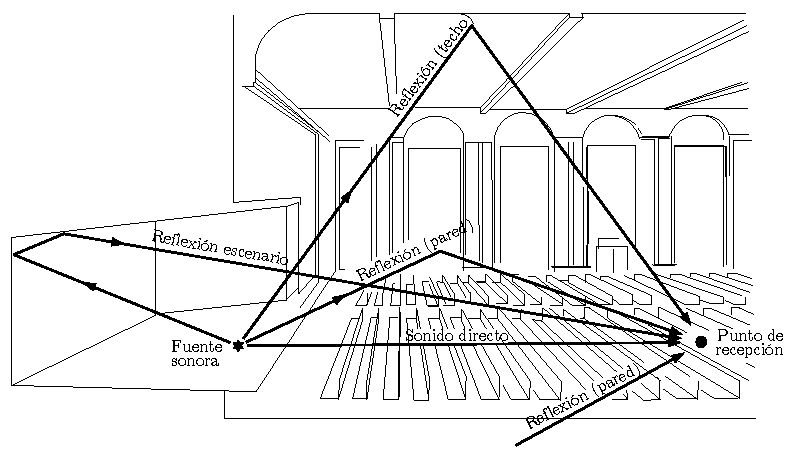
\includegraphics[width=0.7\textwidth]{archivos/geometrica.pdf}
    \caption{Ejemplo de llegada del sonido directo y de las primeras reflexiones a un receptor. Figura extraída y modificada de \cite{Carrión1998}, pág. 51.}
\end{figure}
\FloatBarrier

\subsection{Modos propios}
\label{modospropios}

Las ondas acústicas al reflejarse producen interferencias entre las ondas incidentes y las ondas reflejadas, estas interferencias pueden ser destructivas, reduciendo el nivel de presión acústica o constructivas, aumentando el nivel. Esto es parte de la acústica ondulatoria.

Este efecto, que se produce en posiciones y frecuencias concretas dentro de un recinto, se denomina modos propios. Para facilitar su comprensión se muestra en la figura \ref{graf:ondas} una onda incidente, la onda reflejada y el resultado frente a la distancia. Esto demuestra que es posible tener niveles menores o mayores de lo esperado en algunas posiciones de un recinto.

\begin{figure}[ht]
    \centering
    {\scalefont{0.8}
    %%%%%%%%%%%%%%%%%%%%%%%%%%%%%%%%%%%%%%%%%%%%%%%%%%%%%%%%%%%%%%%%%%%%%%%%
% Escuela Politécnica Superior de la Universidad de Alicante
% Realizado por: Jose Manuel Requena Plens
% Contacto: info@jmrplens.com / Telegram:@jmrplens
%%%%%%%%%%%%%%%%%%%%%%%%%%%%%%%%%%%%%%%%%%%%%%%%%%%%%%%%%%%%%%%%%%%%%%%%

\begin{tikzpicture}

\begin{axis}[%
width=0.5\textwidth,
height=0.15\textwidth,
at={(0\textwidth,0\textwidth)},
scale only axis,
xmin=0,
xmax=8,
xlabel style={font=\color{white!15!black}},
xlabel={Distancia (m)},
ymin=49.5,
ymax=50.5,
ylabel style={font=\color{white!15!black}},
ylabel={Nivel (dB)},
axis background/.style={fill=white},
 axis y line=left,
  axis x line=bottom,
  legend style={at={(0.5,1.05)}, anchor=south, legend cell align=left, align=left, draw=white!15!black,legend columns=-1}
]
\addplot [color=green, line width=1.0pt]
  table[row sep=crcr]{%
0	50\\
0.0638297872340416	50.0295520206661\\
0.106382978723403	50.0479425538604\\
0.148936170212764	50.0644217687238\\
0.170212765957444	50.07173560909\\
0.191489361702125	50.0783326909627\\
0.212765957446805	50.0841470984808\\
0.234042553191486	50.0891207360061\\
0.255319148936174	50.0932039085967\\
0.276595744680854	50.0963558185417\\
0.297872340425535	50.0985449729988\\
0.319148936170215	50.0997494986604\\
0.340425531914896	50.0999573603042\\
0.361702127659576	50.0991664810452\\
0.382978723404257	50.0973847630878\\
0.404255319148938	50.0946300087687\\
0.425531914893618	50.0909297426826\\
0.446808510638299	50.0863209366649\\
0.468085106382979	50.080849640382\\
0.48936170212766	50.0745705212177\\
0.51063829787234	50.0675463180551\\
0.553191489361701	50.0515501371821\\
0.595744680851062	50.0334988150156\\
0.659574468085104	50.0041580662433\\
0.723404255319146	49.9744458897973\\
0.765957446808514	49.9557479556705\\
0.808510638297875	49.9388142109057\\
0.829787234042556	49.9312233840816\\
0.851063829787236	49.9243197504692\\
0.872340425531917	49.9181722888936\\
0.893617021276597	49.9128424227586\\
0.914893617021278	49.9083834063251\\
0.936170212765958	49.904839792611\\
0.957446808510639	49.9022469882335\\
0.978723404255319	49.9006308996367\\
1	49.9000076742436\\
1.02127659574468	49.9003835391164\\
1.04255319148936	49.9017547387376\\
1.06382978723404	49.9041075725337\\
1.08510638297872	49.9074185317672\\
1.1063829787234	49.911654534428\\
1.12765957446808	49.9167732557776\\
1.14893617021276	49.9227235512444\\
1.17021276595744	49.929445967443\\
1.19148936170212	49.9368733362128\\
1.23404255319149	49.9535397820586\\
1.27659574468085	49.9720584501801\\
1.3404255319149	50.0016813900484\\
1.40425531914894	50.0311541363513\\
1.4468085106383	50.0494113351139\\
1.48936170212766	50.0656986598719\\
1.51063829787234	50.0728969040126\\
1.53191489361702	50.0793667863849\\
1.5531914893617	50.0850436620629\\
1.57446808510638	50.0898708095812\\
1.59574468085106	50.0937999976775\\
1.61702127659574	50.0967919672031\\
1.63829787234042	50.0988168233877\\
1.6595744680851	50.0998543345375\\
1.68085106382978	50.099894134184\\
1.70212765957447	50.0989358246623\\
1.72340425531915	50.0969889810845\\
1.74468085106383	50.094073055668\\
1.76595744680851	50.0902171833756\\
1.78723404255319	50.0854598908088\\
1.80851063829788	50.0798487112624\\
1.82978723404256	50.0734397097874\\
1.85106382978724	50.0662969230082\\
1.8936170212766	50.0501020856458\\
1.93617021276596	50.0319098362349\\
2	50.0024775425453\\
2.06382978723404	49.9728239373589\\
2.1063829787234	49.9542464106225\\
2.14893617021276	49.9374929351107\\
2.17021276595744	49.9300125312406\\
2.19148936170212	49.9232314190236\\
2.21276595744681	49.9172173530914\\
2.23404255319149	49.9120304240028\\
2.25531914893617	49.9077224578387\\
2.27659574468085	49.904336498373\\
2.29787234042553	49.9019063769934\\
2.31914893617022	49.9004563746694\\
2.3404255319149	49.9000009793449\\
2.36170212765958	49.9005447411796\\
2.38297872340426	49.9020822270849\\
2.40425531914894	49.9045980750098\\
2.42553191489362	49.9080671474335\\
2.4468085106383	49.9124547825312\\
2.46808510638298	49.9177171405031\\
2.48936170212766	49.9238016416081\\
2.51063829787234	49.9306474915223\\
2.53191489361702	49.9381862887763\\
2.57446808510638	49.9550352535465\\
2.61702127659574	49.9736768208634\\
2.70212765957447	50.013323204142\\
2.74468085106383	50.0327474439138\\
2.78723404255319	50.0508661464372\\
2.82978723404256	50.0669569762197\\
2.85106382978724	50.0740375889952\\
2.87234042553192	50.0803784426552\\
2.8936170212766	50.0859161814857\\
2.91489361702128	50.0905954742308\\
2.93617021276596	50.0943695669444\\
2.95744680851064	50.0972007501395\\
2.97872340425532	50.0990607355695\\
3	50.0999309388748\\
3.02127659574468	50.0998026652716\\
3.04255319148936	50.0986771964275\\
3.06382978723404	50.0965657776549\\
3.08510638297872	50.0934895055525\\
3.1063829787234	50.089479117214\\
3.12765957446808	50.0845746831143\\
3.14893617021276	50.0788252067375\\
3.17021276595744	50.0722881349512\\
3.19148936170212	50.0650287840157\\
3.23404255319149	50.0486398688854\\
3.27659574468085	50.0303118356746\\
3.3404255319149	50.0007963183786\\
3.40425531914894	49.9712096683335\\
3.4468085106383	49.9527578013601\\
3.48936170212766	49.9361893317652\\
3.51063829787234	49.9288214657631\\
3.53191489361702	49.9221647921466\\
3.5531914893617	49.916285822198\\
3.57446808510638	49.9112432966418\\
3.59574468085106	49.9070875987266\\
3.61702127659574	49.903860250812\\
3.63829787234042	49.9015934994918\\
3.6595744680851	49.9003099933958\\
3.68085106382978	49.9000225568927\\
3.70212765957447	49.9007340619529\\
3.72340425531915	49.9024373994532\\
3.74468085106383	49.9051155502082\\
3.76595744680851	49.9087417550209\\
3.78723404255319	49.9132797820514\\
3.80851063829788	49.9186842888339\\
3.82978723404256	49.9249012753228\\
3.85106382978724	49.9318686234445\\
3.8936170212766	49.9477691410373\\
3.93617021276596	49.965751938153\\
3.97872340425532	49.9851000974186\\
4.08510638297872	50.034331492882\\
4.12765957446808	50.0523065765158\\
4.17021276595744	50.0681963620068\\
4.19148936170212	50.0751573415352\\
4.21276595744681	50.0813673737507\\
4.23404255319149	50.0867644100642\\
4.25531914893617	50.0912945250728\\
4.27659574468085	50.0949124553648\\
4.29787234042553	50.0975820517767\\
4.31914893617022	50.0992766405836\\
4.3404255319149	50.0999792900143\\
4.36170212765958	50.0996829794279\\
4.38297872340426	50.0983906694619\\
4.40425531914894	50.0961152724502\\
4.42553191489362	50.0928795234077\\
4.4468085106383	50.0887157528692\\
4.46808510638298	50.0836655638536\\
4.48936170212766	50.0777794161801\\
4.51063829787234	50.0711161222906\\
4.53191489361702	50.063742259615\\
4.57446808510638	50.0471639003094\\
4.61702127659574	50.0287052651328\\
4.68085106382978	49.999114869071\\
4.74468085106383	49.9696035391189\\
4.78723404255319	49.951282548754\\
4.82978723404256	49.9349037694334\\
4.85106382978724	49.9276505243956\\
4.87234042553192	49.9211201714025\\
4.8936170212766	49.9153779595825\\
4.91489361702128	49.910481263218\\
4.93617021276596	49.9064790084805\\
4.95744680851064	49.9034111845764\\
4.97872340425532	49.9013084441879\\
5	49.9001917972021\\
5.02127659574468	49.9000724007863\\
5.04255319148936	49.9009514479103\\
5.06382978723404	49.9028201554256\\
5.08510638297872	49.9056598518245\\
5.1063829787234	49.9094421637993\\
5.12765957446808	49.914129299739\\
5.14893617021276	49.9196744273306\\
5.17021276595744	49.9260221414922\\
5.19148936170212	49.9331090179622\\
5.23404255319149	49.9492103409609\\
5.27659574468085	49.9673364873895\\
5.3404255319149	49.9967264620669\\
5.40425531914894	50.0264088521384\\
5.4468085106383	50.0450440594275\\
5.48936170212766	50.061883502212\\
5.51063829787234	50.0694164668252\\
5.53191489361702	50.076255845048\\
5.5531914893617	50.0823333000738\\
5.57446808510638	50.0875881079811\\
5.59574468085106	50.0919677644662\\
5.61702127659574	50.0954285094493\\
5.63829787234042	50.0979357643104\\
5.6595744680851	50.0994644773878\\
5.68085106382978	50.0999993742857\\
5.70212765957447	50.0995351104912\\
5.72340425531915	50.0980763247745\\
5.74468085106383	50.0956375928404\\
5.76595744680851	50.0922432816923\\
5.78723404255319	50.0879273061651\\
5.80851063829788	50.0827327900595\\
5.82978723404256	50.0767116352635\\
5.85106382978724	50.0699240031655\\
5.87234042553192	50.0624377135416\\
5.91489361702128	50.0456745972144\\
5.95744680851064	50.0270905788308\\
6.02127659574468	49.9974336700139\\
6.08510638297872	49.9680060038116\\
6.12765957446808	49.9498210698979\\
6.17021276595744	49.9336366115787\\
6.19148936170212	49.9265000381951\\
6.21276595744681	49.920097852134\\
6.23404255319149	49.9144940219223\\
6.25531914893617	49.909744539179\\
6.27659574468085	49.9058968591657\\
6.29787234042553	49.9029894266293\\
6.31914893617022	49.9010512916745\\
6.3404255319149	49.9001018195053\\
6.36170212765958	49.9001504969336\\
6.38297872340426	49.9011968375907\\
6.40425531914894	49.9032303867866\\
6.42553191489362	49.90623082597\\
6.4468085106383	49.9101681757443\\
6.46808510638298	49.9150030954121\\
6.48936170212766	49.9206872760543\\
6.51063829787234	49.9271639232168\\
6.53191489361702	49.9343683243822\\
6.57446808510638	49.9506659005043\\
6.61702127659574	49.9689302714906\\
6.68085106382978	49.99840741374\\
6.74468085106383	50.0280268169769\\
6.78723404255319	50.0465388476355\\
6.82978723404256	50.0631955213007\\
6.85106382978724	50.070616945718\\
6.87234042553192	50.0773327889566\\
6.8936170212766	50.0832759485308\\
6.91489361702128	50.0883870423546\\
6.93617021276596	50.0926150020681\\
6.95744680851064	50.0959175832953\\
6.97872340425532	50.0982617877364\\
7	50.0996241928755\\
7.02127659574468	50.0999911860107\\
7.04255319148936	50.099359100268\\
7.06382978723404	50.0977342512392\\
7.08510638297872	50.0951328738787\\
7.1063829787234	50.0915809602891\\
7.12765957446808	50.0871140000169\\
7.14893617021276	50.0817766254526\\
7.17021276595744	50.0756221658786\\
7.19148936170213	50.0687121146205\\
7.21276595744681	50.0611155146263\\
7.25531914893617	50.0441723806669\\
7.29787234042553	50.0254682332844\\
7.4468085106383	49.9571817330504\\
7.48936170212766	49.9400816550786\\
7.51063829787234	49.9323882164612\\
7.53191489361702	49.9253703324355\\
7.5531914893617	49.9190981233788\\
7.57446808510638	49.9136342591307\\
7.59574468085106	49.9090333328166\\
7.61702127659574	49.9053413153715\\
7.63829787234042	49.9025950962132\\
7.6595744680851	49.9008221146557\\
7.68085106382978	49.9000400857447\\
7.70212765957447	49.9002568232546\\
};
\addlegendentry{Onda incidente}

\addplot [color=blue, line width=1.0pt]
  table[row sep=crcr]{%
0	50.05\\
0.0425531914893611	50.0662085976342\\
0.0638297872340416	50.0733596250863\\
0.0851063829787222	50.079777667414\\
0.106382978723403	50.0853985976599\\
0.127659574468083	50.0901662533471\\
0.148936170212764	50.0940329976357\\
0.170212765957444	50.0969601952952\\
0.191489361702125	50.0989185987341\\
0.212765957446805	50.0998886402325\\
0.234042553191486	50.0998606274566\\
0.255319148936174	50.0988348403006\\
0.276595744680854	50.0968215280908\\
0.297872340425535	50.0938408071773\\
0.319148936170215	50.0899224599381\\
0.340425531914896	50.0851056372036\\
0.361702127659576	50.0794384670743\\
0.382978723404257	50.0729775740409\\
0.404255319148938	50.0657875132109\\
0.446808510638299	50.0495138188003\\
0.48936170212766	50.031266164684\\
0.553191489361701	50.0017992906999\\
0.617021276595743	49.9721716914363\\
0.659574468085104	49.9536442334837\\
0.702127659574465	49.936964833658\\
0.723404255319146	49.9295295817644\\
0.744680851063826	49.9227984469954\\
0.765957446808514	49.9168386846246\\
0.787234042553195	49.9117098426275\\
0.808510638297875	49.907463166698\\
0.829787234042556	49.9041410882183\\
0.851063829787236	49.9017768002984\\
0.872340425531917	49.9003939261216\\
0.893617021276597	49.9000062829096\\
0.914893617021278	49.9006177438653\\
0.936170212765958	49.9022221994729\\
0.957446808510639	49.9048036185422\\
0.978723404255319	49.9083362083874\\
1	49.9127846725383\\
1.02127659574468	49.9181045634117\\
1.04255319148936	49.9242427264164\\
1.06382978723404	49.9311378310568\\
1.08510638297872	49.9387209837264\\
1.12765957446808	49.9556422420381\\
1.17021276595744	49.9743319041807\\
1.31914893617022	50.0426313514886\\
1.36170212765958	50.0597527031571\\
1.38297872340426	50.067459318741\\
1.40425531914894	50.0744919031112\\
1.42553191489362	50.0807801890092\\
1.4468085106383	50.086261345961\\
1.46808510638298	50.0908806080582\\
1.48936170212766	50.0945918211608\\
1.51063829787234	50.0973579040543\\
1.53191489361702	50.0991512189527\\
1.5531914893617	50.0999538476463\\
1.57446808510638	50.0997577705347\\
1.59574468085106	50.0985649467554\\
1.61702127659574	50.0963872946093\\
1.63829787234042	50.0932465724769\\
1.6595744680851	50.0891741614156\\
1.68085106382978	50.0842107516104\\
1.70212765957447	50.0784059358115\\
1.72340425531915	50.0718177138196\\
1.74468085106383	50.0645119129709\\
1.78723404255319	50.0480460037393\\
1.82978723404256	50.0296646519565\\
1.8936170212766	50.0001179184898\\
1.95744680851064	49.9705606517156\\
2	49.9521609626815\\
2.04255319148936	49.9356684651004\\
2.06382978723404	49.9283465953864\\
2.08510638297872	49.9217406628059\\
2.1063829787234	49.9159166716535\\
2.12765957446808	49.9109328133237\\
2.14893617021276	49.9068388848814\\
2.17021276595744	49.9036757915065\\
2.19148936170212	49.9014751377822\\
2.21276595744681	49.9002589119133\\
2.23404255319149	49.9000392660265\\
2.25531914893617	49.9008183947509\\
2.27659574468085	49.90258851329\\
2.29787234042553	49.9053319352042\\
2.31914893617022	49.9090212491288\\
2.3404255319149	49.9136195926585\\
2.36170212765958	49.9190810206649\\
2.38297872340426	49.9253509643644\\
2.40425531914894	49.9323667765524\\
2.4468085106383	49.9483488556298\\
2.48936170212766	49.9663901028386\\
2.5531914893617	49.9957241201395\\
2.61702127659574	50.0254400890537\\
2.6595744680851	50.0441462691656\\
2.70212765957447	50.0610924768375\\
2.72340425531915	50.0686909672612\\
2.74468085106383	50.0756031202463\\
2.76595744680851	50.081759871845\\
2.78723404255319	50.0870997058304\\
2.80851063829788	50.0915692683465\\
2.82978723404256	50.095123901002\\
2.85106382978724	50.0977280870825\\
2.87234042553192	50.0993558064215\\
2.8936170212766	50.0999907953854\\
2.91489361702128	50.0996267093743\\
2.93617021276596	50.0982671862154\\
2.95744680851064	50.0959258098147\\
2.97872340425532	50.0926259744311\\
3	50.0884006509291\\
3.02127659574468	50.0832920573444\\
3.04255319148936	50.0773512370554\\
3.06382978723404	50.0706375487747\\
3.08510638297872	50.0632180734562\\
3.12765957446808	50.0465646047645\\
3.17021276595744	50.028054752224\\
3.23404255319149	49.9984365129409\\
3.29787234042553	49.9689579353004\\
3.3404255319149	49.9506912172779\\
3.38297872340426	49.9343902848196\\
3.40425531914894	49.9271838673773\\
3.42553191489362	49.9207050046622\\
3.4468085106383	49.9150184313292\\
3.46808510638298	49.9101809657391\\
3.48936170212766	49.9062409422491\\
3.51063829787234	49.9032377282716\\
3.53191489361702	49.9012013309278\\
3.5531914893617	49.9001520972269\\
3.57446808510638	49.9001005107651\\
3.59574468085106	49.9010470869774\\
3.61702127659574	49.9029823679872\\
3.63829787234042	49.9058870171062\\
3.6595744680851	49.9097320120408\\
3.68085106382978	49.9144789348723\\
3.70212765957447	49.9200803559172\\
3.72340425531915	49.9264803076278\\
3.74468085106383	49.9336148438021\\
3.78723404255319	49.9497958983742\\
3.82978723404256	49.96797843205\\
3.8936170212766	49.9974045768834\\
3.95744680851064	50.027062563134\\
4	50.04564870549\\
4.04255319148936	50.062414978011\\
4.06382978723404	50.0699031949744\\
4.08510638297872	50.0766929623205\\
4.1063829787234	50.0827164389384\\
4.12765957446808	50.0879134402409\\
4.14893617021276	50.0922320395088\\
4.17021276595744	50.0956290867259\\
4.19148936170212	50.0980706397191\\
4.21276595744681	50.0995323032981\\
4.23404255319149	50.0999994730035\\
4.25531914893617	50.0994674810301\\
4.27659574468085	50.0979416428659\\
4.29787234042553	50.0954372041813\\
4.31914893617022	50.0919791884999\\
4.3404255319149	50.0876021471713\\
4.36170212765958	50.0823498141455\\
4.38297872340426	50.0762746689981\\
4.40425531914894	50.0694374125711\\
4.42553191489362	50.0619063604706\\
4.46808510638298	50.045070040708\\
4.51063829787234	50.026436920649\\
4.59574468085106	49.9867936723521\\
4.63829787234042	49.9673639953223\\
4.68085106382978	49.94923541281\\
4.72340425531915	49.9331306541922\\
4.74468085106383	49.9260417264718\\
4.76595744680851	49.9196917653732\\
4.78723404255319	49.9141442176086\\
4.80851063829788	49.9094545124415\\
4.82978723404256	49.9056695078558\\
4.85106382978724	49.902827022366\\
4.87234042553192	49.9009554571476\\
4.8936170212766	49.9000735122617\\
4.91489361702128	49.9001899998099\\
4.93617021276596	49.9013037558872\\
4.95744680851064	49.9034036522111\\
4.97872340425532	49.9064687073115\\
5	49.9104682961712\\
5.02127659574468	49.9153624562203\\
5.04255319148936	49.9211022866293\\
5.06382978723404	49.9276304369103\\
5.08510638297872	49.9348816799434\\
5.12765957446808	49.9512571351854\\
5.17021276595744	49.9695758146306\\
5.23404255319149	49.9990857674241\\
5.29787234042553	50.0286773858907\\
5.3404255319149	50.0471382356822\\
5.38297872340426	50.0637198327704\\
5.40425531914894	50.0710956591506\\
5.42553191489362	50.0777611212056\\
5.4468085106383	50.083649619842\\
5.46808510638298	50.0887023191277\\
5.48936170212766	50.0928687341619\\
5.51063829787234	50.0961072355026\\
5.53191489361702	50.098385465115\\
5.5531914893617	50.0996806596819\\
5.57446808510638	50.0999798780473\\
5.59574468085106	50.0992801305202\\
5.61702127659574	50.0975884087466\\
5.63829787234042	50.0949216158512\\
5.6595744680851	50.0913063975472\\
5.68085106382978	50.0867788759007\\
5.70212765957447	50.0813842884115\\
5.72340425531915	50.0751765360146\\
5.74468085106383	50.0682176445199\\
5.78723404255319	50.0523313784145\\
5.82978723404256	50.034358825393\\
5.87234042553192	50.0150164944285\\
5.97872340425532	49.9657792824314\\
6.02127659574468	49.9477939608735\\
6.06382978723404	49.9318899293498\\
6.08510638297872	49.9249204955844\\
6.1063829787234	49.9187012314092\\
6.12765957446808	49.9132942776559\\
6.14893617021276	49.9087536588192\\
6.17021276595744	49.9051247432615\\
6.19148936170212	49.9024437899076\\
6.21276595744681	49.9007375859571\\
6.23404255319149	49.9000231792359\\
6.25531914893617	49.9003077078599\\
6.27659574468085	49.901588328913\\
6.29787234042553	49.9038522468531\\
6.31914893617022	49.9070768413604\\
6.3404255319149	49.9112298933525\\
6.36170212765958	49.9162699069068\\
6.38297872340426	49.9221465238737\\
6.40425531914894	49.9288010270391\\
6.42553191489362	49.9361669268072\\
6.46808510638298	49.9527321529319\\
6.51063829787234	49.971181798957\\
6.57446808510638	50.0007672164432\\
6.63829787234042	50.0302841007695\\
6.68085106382978	50.0486144386115\\
6.72340425531915	50.0650066721979\\
6.74468085106383	50.0722680226478\\
6.76595744680851	50.0788072949041\\
6.78723404255319	50.0845591507199\\
6.80851063829788	50.0894661194533\\
6.82978723404256	50.0934791722947\\
6.85106382978724	50.0965582121466\\
6.87234042553192	50.0986724742606\\
6.8936170212766	50.0998008336286\\
6.91489361702128	50.0999320160568\\
6.93617021276596	50.0990647108136\\
6.95744680851064	50.0972075837265\\
6.97872340425532	50.0943791905953\\
7	50.0906077917893\\
7.02127659574468	50.0859310698787\\
7.04255319148936	50.0803957531229\\
7.06382978723404	50.0740571485772\\
7.08510638297872	50.0669785894829\\
7.12765957446808	50.0508912008434\\
7.17021276595744	50.0327749406228\\
7.23404255319149	50.003391390949\\
7.29787234042553	49.9737048984222\\
7.3404255319149	49.9550612502714\\
7.38297872340426	49.9382091682599\\
7.40425531914894	49.9306684610792\\
7.42553191489362	49.9238204917176\\
7.4468085106383	49.917733682821\\
7.46808510638298	49.9124688517721\\
7.48936170212766	49.9080786030224\\
7.51063829787234	49.904606802486\\
7.53191489361702	49.9020881392465\\
7.5531914893617	49.9005477789542\\
7.57446808510638	49.9000011123801\\
7.59574468085106	49.9004536016358\\
7.61702127659574	49.9019007255983\\
7.63829787234042	49.9043280250834\\
7.6595744680851	49.9077112473168\\
7.68085106382978	49.9120165882605\\
7.70212765957447	49.9172010303708\\
};
\addlegendentry{Onda reflejada}

\addplot [color=red, line width=1.5pt]
  table[row sep=crcr]{%
0	50.05\\
0.0425531914893611	50.0860755307137\\
0.0638297872340416	50.1029116457524\\
0.0851063829787222	50.1187195016449\\
0.106382978723403	50.1333411515204\\
0.127659574468083	50.1466305006866\\
0.148936170212764	50.1584547663595\\
0.170212765957444	50.1686958043852\\
0.191489361702125	50.1772512896968\\
0.212765957446805	50.1840357387133\\
0.234042553191486	50.1889813634627\\
0.255319148936174	50.1920387488973\\
0.276595744680854	50.1931773466325\\
0.297872340425535	50.1923857801761\\
0.319148936170215	50.1896719585985\\
0.340425531914896	50.1850629975077\\
0.361702127659576	50.1786049481196\\
0.382978723404257	50.1703623371287\\
0.404255319148938	50.1604175219796\\
0.425531914893618	50.1488698679779\\
0.446808510638299	50.1358347554652\\
0.468085106382979	50.1214424269768\\
0.48936170212766	50.1058366859016\\
0.51063829787234	50.0891734596459\\
0.553191489361701	50.053349427882\\
0.595744680851062	50.0153985227823\\
0.659574468085104	49.957802299727\\
0.702127659574465	49.9211902642437\\
0.723404255319146	49.9039754715617\\
0.744680851063826	49.8877201242264\\
0.765957446808514	49.8725866402951\\
0.787234042553195	49.8587262285366\\
0.808510638297875	49.8462773776038\\
0.829787234042556	49.8353644722999\\
0.851063829787236	49.8260965507676\\
0.872340425531917	49.8185662150152\\
0.893617021276597	49.8128487056683\\
0.914893617021278	49.8090011501904\\
0.936170212765958	49.8070619920839\\
0.957446808510639	49.8070506067757\\
0.978723404255319	49.808967108024\\
1	49.8127923467819\\
1.02127659574468	49.8184881025281\\
1.04255319148936	49.825997465154\\
1.06382978723404	49.8352454035905\\
1.08510638297872	49.8461395154936\\
1.1063829787234	49.8585709504985\\
1.12765957446808	49.8724154978157\\
1.14893617021276	49.8875348273049\\
1.17021276595744	49.9037778716237\\
1.19148936170212	49.9209823356424\\
1.23404255319149	49.9575800289031\\
1.36170212765958	50.0714076236421\\
1.38297872340426	50.0889713175498\\
1.40425531914894	50.1056460394625\\
1.42553191489362	50.1212651810708\\
1.4468085106383	50.1356726810749\\
1.46808510638298	50.148724584497\\
1.48936170212766	50.1602904810327\\
1.51063829787234	50.1702548080669\\
1.53191489361702	50.1785180053376\\
1.5531914893617	50.1849975097092\\
1.57446808510638	50.1896285801158\\
1.59574468085106	50.1923649444328\\
1.61702127659574	50.1931792618125\\
1.63829787234042	50.1920633958646\\
1.6595744680851	50.189028495953\\
1.68085106382978	50.1841048857944\\
1.70212765957447	50.1773417604739\\
1.72340425531915	50.1688066949041\\
1.74468085106383	50.1585849686389\\
1.76595744680851	50.1467787137883\\
1.78723404255319	50.1335058945481\\
1.80851063829788	50.1188991285408\\
1.82978723404256	50.1031043617439\\
1.85106382978724	50.0862794102462\\
1.8936170212766	50.0502200041356\\
1.95744680851064	49.9928496431256\\
2	49.9546385052268\\
2.04255319148936	49.9182357869781\\
2.06382978723404	49.9011705327453\\
2.08510638297872	49.8850927498807\\
2.1063829787234	49.8701630822759\\
2.12765957446808	49.8565307022347\\
2.14893617021276	49.8443318199921\\
2.17021276595744	49.8336883227471\\
2.19148936170212	49.8247065568059\\
2.21276595744681	49.8174762650047\\
2.23404255319149	49.8120696900293\\
2.25531914893617	49.8085408525897\\
2.27659574468085	49.8069250116629\\
2.29787234042553	49.8072383121976\\
2.31914893617022	49.8094776237982\\
2.3404255319149	49.8136205720035\\
2.36170212765958	49.8196257618445\\
2.38297872340426	49.8274331914493\\
2.40425531914894	49.8369648515622\\
2.42553191489362	49.848125504986\\
2.4468085106383	49.860803638161\\
2.46808510638298	49.8748725753712\\
2.48936170212766	49.8901917444467\\
2.51063829787234	49.906608081314\\
2.53191489361702	49.9239575593614\\
2.57446808510638	49.9607549464186\\
2.68085106382978	50.0562458753018\\
2.72340425531915	50.0918419497714\\
2.74468085106383	50.1083505641601\\
2.76595744680851	50.1237765755276\\
2.78723404255319	50.1379658522676\\
2.80851063829788	50.1507766198172\\
2.82978723404256	50.1620808772217\\
2.85106382978724	50.1717656760778\\
2.87234042553192	50.1797342490767\\
2.8936170212766	50.185906976871\\
2.91489361702128	50.1902221836052\\
2.93617021276596	50.1926367531599\\
2.95744680851064	50.1931265599542\\
2.97872340425532	50.1916867100006\\
3	50.1883315898039\\
3.02127659574468	50.1830947226161\\
3.04255319148936	50.1760284334829\\
3.06382978723404	50.1672033264296\\
3.08510638297872	50.1567075790087\\
3.1063829787234	50.144646061259\\
3.12765957446808	50.1311392878788\\
3.14893617021276	50.1163222140831\\
3.17021276595744	50.1003428871752\\
3.19148936170212	50.0833609673076\\
3.23404255319149	50.0470763818263\\
3.29787234042553	49.9896046834942\\
3.3404255319149	49.9514875356565\\
3.38297872340426	49.9153044266822\\
3.40425531914894	49.8983935357108\\
3.42553191489362	49.8824978629438\\
3.4468085106383	49.8677762326893\\
3.46808510638298	49.8543757386104\\
3.48936170212766	49.8424302740143\\
3.51063829787234	49.8320591940346\\
3.53191489361702	49.8233661230743\\
3.5531914893617	49.8164379194249\\
3.57446808510638	49.811343807407\\
3.59574468085106	49.808134685704\\
3.61702127659574	49.8068426187992\\
3.63829787234042	49.8074805165981\\
3.6595744680851	49.8100420054366\\
3.68085106382978	49.814501491765\\
3.70212765957447	49.8208144178701\\
3.72340425531915	49.8289177070809\\
3.74468085106383	49.8387303940103\\
3.76595744680851	49.8501544335341\\
3.78723404255319	49.8630756804257\\
3.80851063829788	49.8773650298573\\
3.82978723404256	49.8928797073728\\
3.85106382978724	49.909464695443\\
3.8936170212766	49.9451737179207\\
3.93617021276596	49.9830684912506\\
4	50.0406951414022\\
4.04255319148936	50.0774026989773\\
4.06382978723404	50.0946866157727\\
4.08510638297872	50.1110244552025\\
4.1063829787234	50.1262529749757\\
4.12765957446808	50.1402200167567\\
4.14893617021276	50.1527860264808\\
4.17021276595744	50.1638254487327\\
4.19148936170212	50.1732279812543\\
4.21276595744681	50.1808996770488\\
4.23404255319149	50.1867638830677\\
4.25531914893617	50.1907620061029\\
4.27659574468085	50.1928540982306\\
4.29787234042553	50.193019255958\\
4.31914893617022	50.1912558290835\\
4.3404255319149	50.1875814371855\\
4.36170212765958	50.1820327935734\\
4.38297872340426	50.17466533846\\
4.40425531914894	50.1655526850213\\
4.42553191489362	50.1547858838783\\
4.4468085106383	50.1424725133491\\
4.46808510638298	50.1287356045616\\
4.48936170212766	50.1137124121676\\
4.51063829787234	50.0975530429396\\
4.53191489361702	50.0804189559533\\
4.57446808510638	50.0439194497419\\
4.70212765957447	49.9300240587693\\
4.72340425531915	49.9123970121315\\
4.74468085106383	49.8956452655907\\
4.76595744680851	49.8799361970611\\
4.78723404255319	49.8654267663626\\
4.80851063829788	49.8522619469306\\
4.82978723404256	49.8405732772892\\
4.85106382978724	49.8304775467616\\
4.87234042553192	49.8220756285501\\
4.8936170212766	49.8154514718442\\
4.91489361702128	49.8106712630279\\
4.93617021276596	49.8077827643678\\
4.95744680851064	49.8068148367875\\
4.97872340425532	49.8077771514995\\
5	49.8106600933733\\
5.02127659574468	49.8154348570066\\
5.04255319148936	49.8220537345396\\
5.06382978723404	49.8304505923359\\
5.08510638297872	49.840541531768\\
5.1063829787234	49.8522257275047\\
5.12765957446808	49.8653864349244\\
5.14893617021276	49.8798921565891\\
5.17021276595744	49.8955979561228\\
5.19148936170212	49.9123469063682\\
5.23404255319149	49.948296108385\\
5.27659574468085	49.9863065813994\\
5.3404255319149	50.0438646977492\\
5.38297872340426	50.0803678331241\\
5.40425531914894	50.097504511289\\
5.42553191489362	50.1136669566078\\
5.4468085106383	50.1286936792695\\
5.46808510638298	50.1424345372284\\
5.48936170212766	50.1547522363739\\
5.51063829787234	50.1655237023278\\
5.53191489361702	50.174641310163\\
5.5531914893617	50.1820139597557\\
5.57446808510638	50.1875679860284\\
5.59574468085106	50.1912478949864\\
5.61702127659574	50.1930169181958\\
5.63829787234042	50.1928573801616\\
5.6595744680851	50.1907708749349\\
5.68085106382978	50.1867782501864\\
5.70212765957447	50.1809193989027\\
5.72340425531915	50.1732528607892\\
5.74468085106383	50.1638552373604\\
5.76595744680851	50.1528204265632\\
5.78723404255319	50.1402586845796\\
5.80851063829788	50.126295524183\\
5.82978723404256	50.1110704606565\\
5.85106382978724	50.0947356178022\\
5.87234042553192	50.0774542079702\\
5.91489361702128	50.0407501004329\\
6.04255319148936	49.9270063338173\\
6.06382978723404	49.9095143653311\\
6.08510638297872	49.892926499396\\
6.1063829787234	49.8774084764851\\
6.12765957446808	49.8631153475538\\
6.14893617021276	49.8501899248217\\
6.17021276595744	49.8387613548402\\
6.19148936170212	49.8289438281027\\
6.21276595744681	49.8208354380911\\
6.23404255319149	49.8145172011582\\
6.25531914893617	49.8100522470389\\
6.27659574468085	49.8074851880788\\
6.29787234042553	49.8068416734824\\
6.31914893617022	49.808128133035\\
6.3404255319149	49.8113317128578\\
6.36170212765958	49.8164204038404\\
6.38297872340426	49.8233433614644\\
6.40425531914894	49.8320314138258\\
6.42553191489362	49.8423977527771\\
6.4468085106383	49.8543388012864\\
6.46808510638298	49.867735248344\\
6.48936170212766	49.8824532410792\\
6.51063829787234	49.8983457221738\\
6.53191489361702	49.91525389921\\
6.57446808510638	49.9514331169475\\
6.63829787234042	50.0088588467399\\
6.68085106382978	50.0470218523515\\
6.72340425531915	50.0833102450959\\
6.74468085106383	50.1002948396247\\
6.76595744680851	50.116277321269\\
6.78723404255319	50.1310979983554\\
6.80851063829788	50.1446087875775\\
6.82978723404256	50.1566746935954\\
6.85106382978724	50.1671751578646\\
6.87234042553192	50.1760052632172\\
6.8936170212766	50.1830767821594\\
6.91489361702128	50.1883190584114\\
6.93617021276596	50.1916797128817\\
6.95744680851064	50.1931251670218\\
6.97872340425532	50.1926409783317\\
7	50.1902319846648\\
7.02127659574468	50.1859222558894\\
7.04255319148936	50.1797548533909\\
7.06382978723404	50.1717913998164\\
7.08510638297872	50.1621114633616\\
7.1063829787234	50.1508117627518\\
7.12765957446808	50.1380052008603\\
7.14893617021276	50.1238197366203\\
7.17021276595744	50.1083971065014\\
7.19148936170213	50.0918914083256\\
7.21276595744681	50.0744675615731\\
7.25531914893617	50.0375692299608\\
7.36170212765958	49.9421204655342\\
7.38297872340426	49.9240092461625\\
7.40425531914894	49.9066573012839\\
7.42553191489362	49.8902380057958\\
7.4468085106383	49.8749154158714\\
7.46808510638298	49.8608426297641\\
7.48936170212766	49.8481602581009\\
7.51063829787234	49.8369950189473\\
7.53191489361702	49.827458471682\\
7.5531914893617	49.819645902333\\
7.57446808510638	49.8136353715108\\
7.59574468085106	49.8094869344525\\
7.61702127659574	49.8072420409698\\
7.63829787234042	49.8069231212965\\
7.6595744680851	49.8085333619725\\
7.68085106382978	49.8120566740052\\
7.70212765957447	49.8174578536254\\
};
\addlegendentry{Nivel resultante}
\draw[line width=1.5pt,  pattern=bricks, pattern color=brown] (axis cs:7.7,49) rectangle (axis cs:8,51);
\end{axis}
\end{tikzpicture}%
    }
    \caption{Ejemplo básico de interferencia de ondas (100 Hz) en dos dimensiones frente a la distancia.}
    \label{graf:ondas}
\end{figure}
\FloatBarrier

Los modos propios varían según las dimensiones del recinto, es por ello por lo que se denomina \textit{propio} pues cada recinto producirá unos modos.

Es posible calcular las frecuencias que van a producir un modo propio para un recinto rectangular con:

\begin{flalign}
	f = \frac{c}{2}\sqrt{ \left(\frac{n_x}{L_x}\right)^2 +\left(\frac{n_y}{L_y}\right)^2 +\left(\frac{n_z}{L_z}\right)^2 }
\end{flalign}

\begin{condiciones}[Donde:]
	n_x,n_y,n_z & \rightarrow & Son los índices para cada modo propio. 0,1,2,3,...\\
	L_x,L_y,L_z & \rightarrow & Son las dimensiones del recinto, largo, ancho y alto en metros.\\
	c & \rightarrow & Es la velocidad del sonido en el aire.
\end{condiciones}

Los modos propios en un recinto rectangular pueden ser:
\begin{description}
\itemsep0em
	\item[Axiales:] Son los modos producidos entre dos superficies (techo y suelo, pared izquierda y pared derecha, pared frontal y posterior). Las combinaciones de índices pueden ser: ($n_x$,$0$,$0$) ; ($0$,$n_y$,$0$) ; ($0$,$0$,$n_z$).
	\item[Tangenciales:] Son los modos producidos entre cuatro superficies, es decir, entre aristas enfrentadas (suelo+pared izquierda y techo+pared derecha, ...). Las combinaciones de índices pueden ser: ($n_x$,$n_y$,$0$) ; ($n_x$,$0$,$n_z$) ; ($0$,$n_y$,$n_z$).
	\item[Oblicuos:] Son los modos producidos entre seis superficies, es decir, vértices enfrentados. Las combinaciones de índices pueden ser: ($n_x$,$n_y$,$n_z$).
\end{description}

La diferencia de nivel en distintas posiciones se va reduciendo cuando la densidad modal (número de modos en una frecuencia o banda de frecuencia) aumenta, llegando a ser imperceptible. El cálculo de la densidad modal desde 0 a una frecuencia determinado por \cite{Morse1968} se obtiene como:
\begin{flalign}
	Dn (f) = \frac{4\pi Vf^3}{3c^3} + \frac{\pi S f^2}{4c^2} + \frac{Lf}{8c}
\end{flalign}
\begin{condiciones}[Donde:]
	V & \rightarrow & Es el volumen del recinto en $m^3$.\\
	S & \rightarrow & Es la superficie del recinto en $m^2$.\\
	L & \rightarrow & Es el perímetro del recinto en $m$.\\
	f & \rightarrow & Es la frecuencia límite para el cálculo.
\end{condiciones}

Derivando esta ecuación como indica \cite{Mankovsky1971} se puede obtener la densidad modal para una frecuencia concreta:
\begin{flalign}
	Dn(f_i) = \frac{4\pi Vf_i^2}{3c^3} + \frac{\pi S f_i}{4c^2} + \frac{L}{8c}
\end{flalign}

Se puede obtener una aproximación de la densidad modal en una banda de octava o tercio de octava completa mediante:
\begin{flalign}
	Dn(f_i,\Delta f_i) = \left( \frac{4\pi Vf_i^2}{3c^3} + \frac{\pi S f_i}{4c^2} + \frac{L}{8c} \right) \Delta f_i \label{ecu:densmodal}
\end{flalign}
\begin{condiciones}[Donde:]
	f_i & \rightarrow & Es la frecuencia central de la banda.\\
	\Delta f_i & \rightarrow & Es el ancho de la banda.
\end{condiciones}

Es posible conocer a partir de que frecuencia la respuesta modal no será apreciable por una persona (debido al número de modos que contiene) y por tanto más allá de esa frecuencia no tiene importancia estudiar la respuesta modal. El cálculo, definido por \cite{schroeder1954}, tenía en cuenta a partir de qué frecuencia se producían mínimo 10 modos en todas las bandas y revisado en \cite{Schroeder1962} donde aclaró que era suficiente con 3 modos. Debido al estudio de Schroeder la ecuación recibió el nombre de \textit{frecuencia de Schroeder} también conocida como frecuencia límite o de cruce:
\begin{flalign}
	f_s = 2000 \sqrt{\frac{T}{V}}\label{ecu:schroeder}
\end{flalign}
\begin{condiciones}[Donde:]
	T & \rightarrow & Es el tiempo medio de reverberación (entre 500 Hz y 1 KHz) en segundos.\\
	V & \rightarrow & Es el volumen del recinto en $m^3$.
\end{condiciones}

\subsection{Coeficiente de absorción medio}
\label{coefmedioabs}
La absorción acústica es la disipación de la energía acústica al paso de ésta por un material. Los materiales absorbentes son diseñados para producir esta disipación a ciertas frecuencias sobre las que se desea actuar. Debido a que el propósito de este trabajo no es profundizar en el funcionamiento y diseño de estos materiales, si se tiene interés se recomienda la lectura de \cite{Cox2016}, donde se desarrollan todos los conceptos sobre los materiales para el acondicionamiento acústico de recintos.

El coeficiente de absorción de los materiales se suele ofrecer u obtener por bandas de frecuencia, pero en algunos cálculos es necesario un coeficiente global, en el documento DB-HR del Código Técnico de la Edificación (\textit{sección 3.2}) se indica que este coeficiente se obtiene realizando el promedio del coeficiente de absorción en las bandas de 500 Hz, 1000 Hz y 2000 Hz (ecuación \ref{ecu:coefmedio}). Estos coeficientes no tienen unidades y comprenden un valor entre 0 y 1, donde 0 es reflexión total y 1 es la absorción total.

\begin{flalign}
 	\alpha_{mid} =& \frac{\alpha_{500}+\alpha_{1000}+\alpha_{2000}}{3}\label{ecu:coefmedio}
 \end{flalign}

\subsection{Absorción acústica}

Para los cálculos acústicos, en ocasiones, se utiliza el valor de absorción total o equivalente del recinto; éste se calcula como la suma de las áreas de absorción por su coeficiente de absorción (medio o por bandas). Las unidades de absorción son los $m^2$.

\begin{flalign}
	A_T = \sum_{i=1}^n S_i \alpha_i
\end{flalign}
\begin{condiciones}[Donde:]
S_i & \rightarrow & Es la superficie del material $i$ en $m^2$.\\
\alpha_i & \rightarrow & Es el coeficiente de absorción del material $i$, no tiene unidades. El valor se encuentra entre $0$ y $1$.	
\end{condiciones}

\subsection{Constante del recinto}
 La constante del recinto es un valor que relaciona la absorción media de las superficies del recinto y el área. Se representa con las letras $Rc$ provenientes de \textit{room constant} y sus unidades son los $m^2$.
 
 \begin{flalign}
 	Rc =& \frac{A_T}{1-\overline{\alpha}}
 \end{flalign}
\begin{condiciones}[Donde:]
	\overline{\alpha} & = & $\nicefrac{A_T}{S}$, es el coeficiente medio de absorción, no confundir con coeficiente de absorción medio (\ref{coefmedioabs}).\\
	S & \rightarrow & Es el área total de todas las superficies.
\end{condiciones}

\subsection{Camino libre medio en acústica}

El camino libre medio (en inglés \textit{mean free path}) o MFP aplicado a la acústica geométrica, describe la distancia media que recorre el sonido entre una reflexión y otra.
\cite{jager1911theorie} propuso utilizar una modificación de la teoría cinética de los gases \cite[][cap. 10]{Bernoulli1738a}, obteniendo así el valor del camino libre medio para ondas acústicas como:

\begin{flalign}
	\text{MFP}=4\frac{V}{S}
\end{flalign}
\begin{condiciones}[Donde:]
	V & \rightarrow & Es el volumen del recinto en $m^3$.\\
	S & \rightarrow & Es la suma del área de todas las superficies del recinto en $m^2$.
\end{condiciones}

\citeauthor{jager1911theorie} demostró teóricamente que este valor para MFP es válido para cualquier factor de forma de recinto en el supuesto de que la distribución de energía acústica sea uniforme.
Años más tarde, \cite{Schuster1929} y \cite{Eyring1930} obtuvieron otros valores de MFP para recintos con factores de forma muy concretos:
\begin{flalign*}
	&&\text{Cubo } &\rightarrow \text{MFP}=2\sqrt{3}\frac{V}{S}&&\\
	&&\text{Cilindro (altura=diámetro)} &\rightarrow \text{MFP}=3\sqrt{2}\frac{V}{S}&&\\
	&&\text{Esfera }&\rightarrow \text{MFP}=\text{diámetro}=6\frac{V}{S}&&
\end{flalign*}

\begin{figure}[ht]
    \centering
    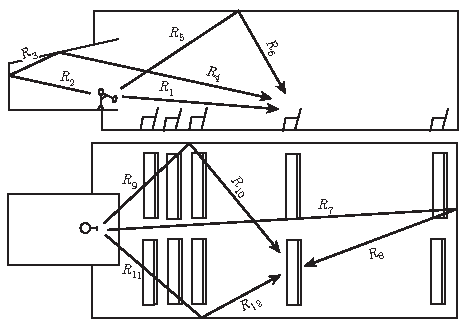
\includegraphics[width=0.8\textwidth]{archivos/mfp.pdf}
    \caption{Trazado de rayos para calcular el camino libre medio (promedio de $R_i$). Figura extraída y modificada de \cite{Self2009}, pág. 109.}
\end{figure}

Poco después, \cite{Knudsen1932} demostró empíricamente (figuras \ref{fig:knudsen1} y \ref{fig:knudsen2}) que el valor de MFP propuesto por \citeauthor{jager1911theorie} no es excesivamente dependiente del factor de forma del recinto. Lo realizó emitiendo rayos lumínicos simulando la emisión de una fuente acústica sobre varios modelos de auditorios a escala, promediando la longitud entre reflexión y reflexión de estos rayos; determinó que el valor $4V/S$ es una buena aproximación del camino libre medio.
 
%\begin{figure}[ht]
%    \centering
%    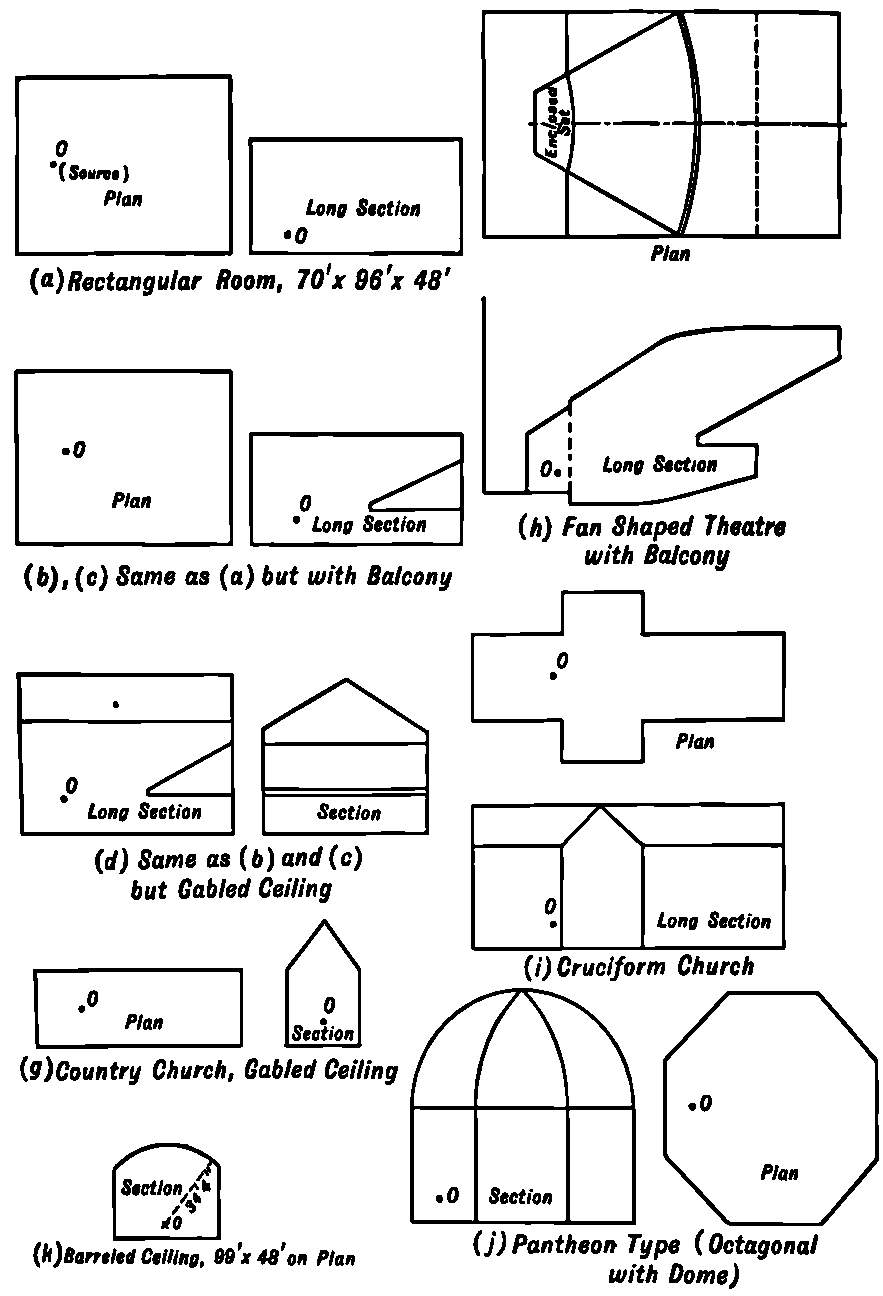
\includegraphics[width=0.5\textwidth]{archivos/mfpknudsen1.pdf}
%    \caption{Modelos utilizados para el cálculo de MFP por Vern O. Knudsen. Figura extraída del libro \cite{Knudsen1932}, pág. 140.}
%    \label{fig:knudsen1}
%\end{figure}
%\FloatBarrier
%\begin{figure}[ht]
%    \centering
%    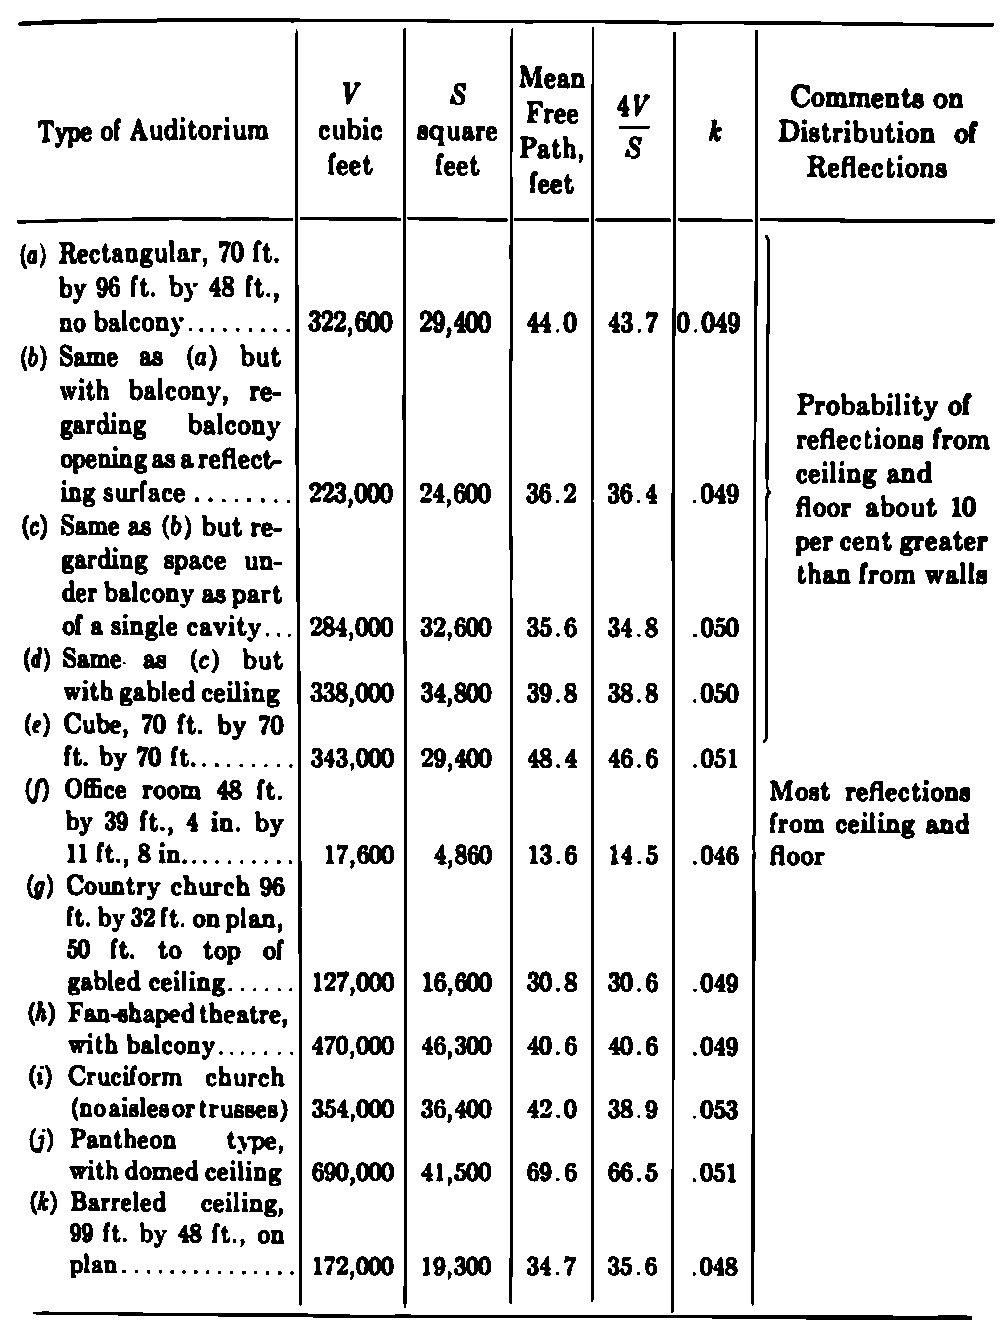
\includegraphics[width=0.5\textwidth]{archivos/mfpknudsen2.pdf}
%    \caption{Resultados obtenidos con el cálculo de MFP por Vern O. Knudsen. Tabla extraída del libro \cite{Knudsen1932}, pág. 141.}
%    \label{fig:knudsen2}
%\end{figure}
%\FloatBarrier
\begin{figure}[ht]
    \centering
    \begin{subfigure}[b]{0.48\textwidth}
    	\centering
        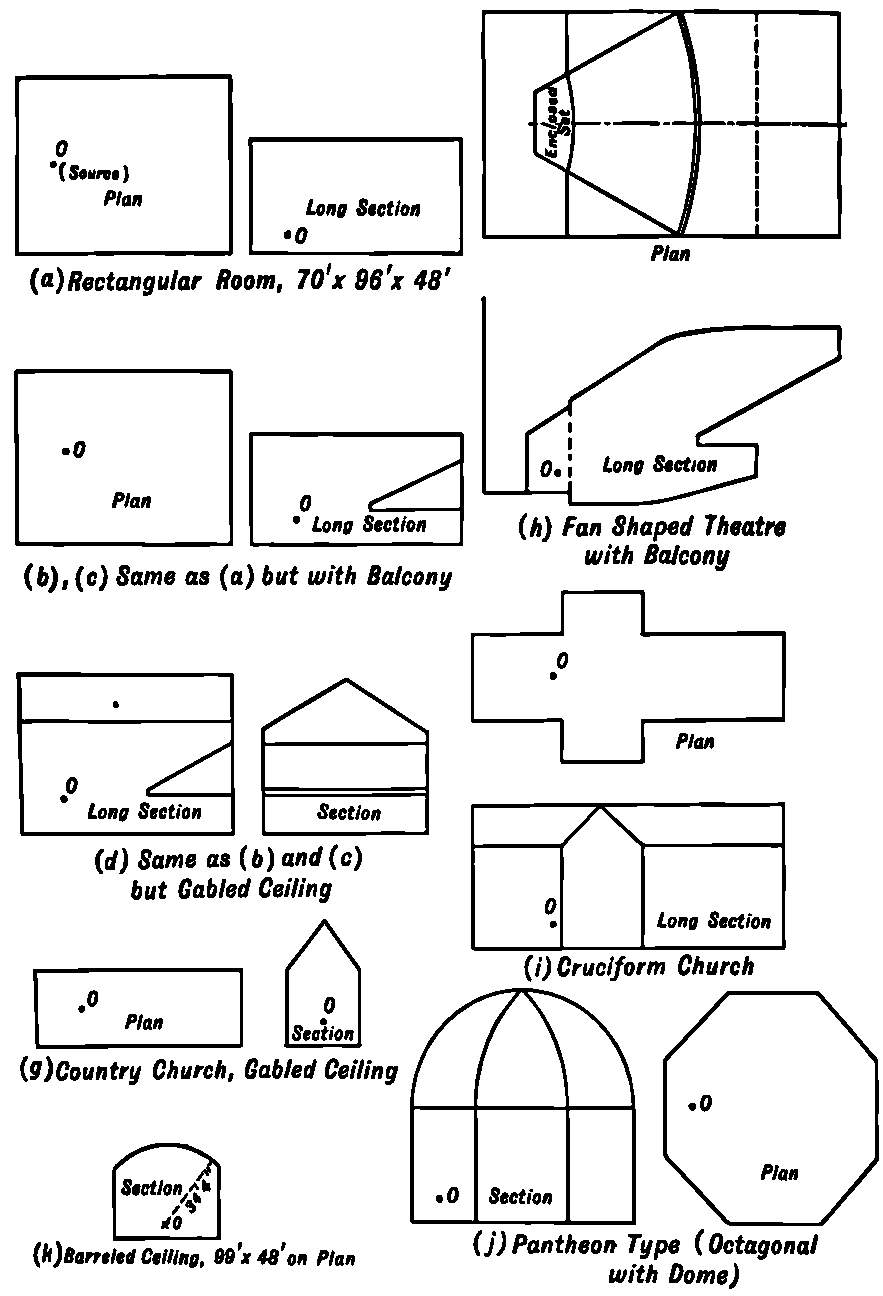
\includegraphics[width=0.9\linewidth]{archivos/mfpknudsen1.pdf}
        \caption{}
        \label{fig:knudsen1}
    \end{subfigure}
    ~ % Añadir el espacio deseado, si se deja la linea en blanco la siguiente subfigura ira en una nueva linea
    \begin{subfigure}[b]{0.48\textwidth}
    	\centering
        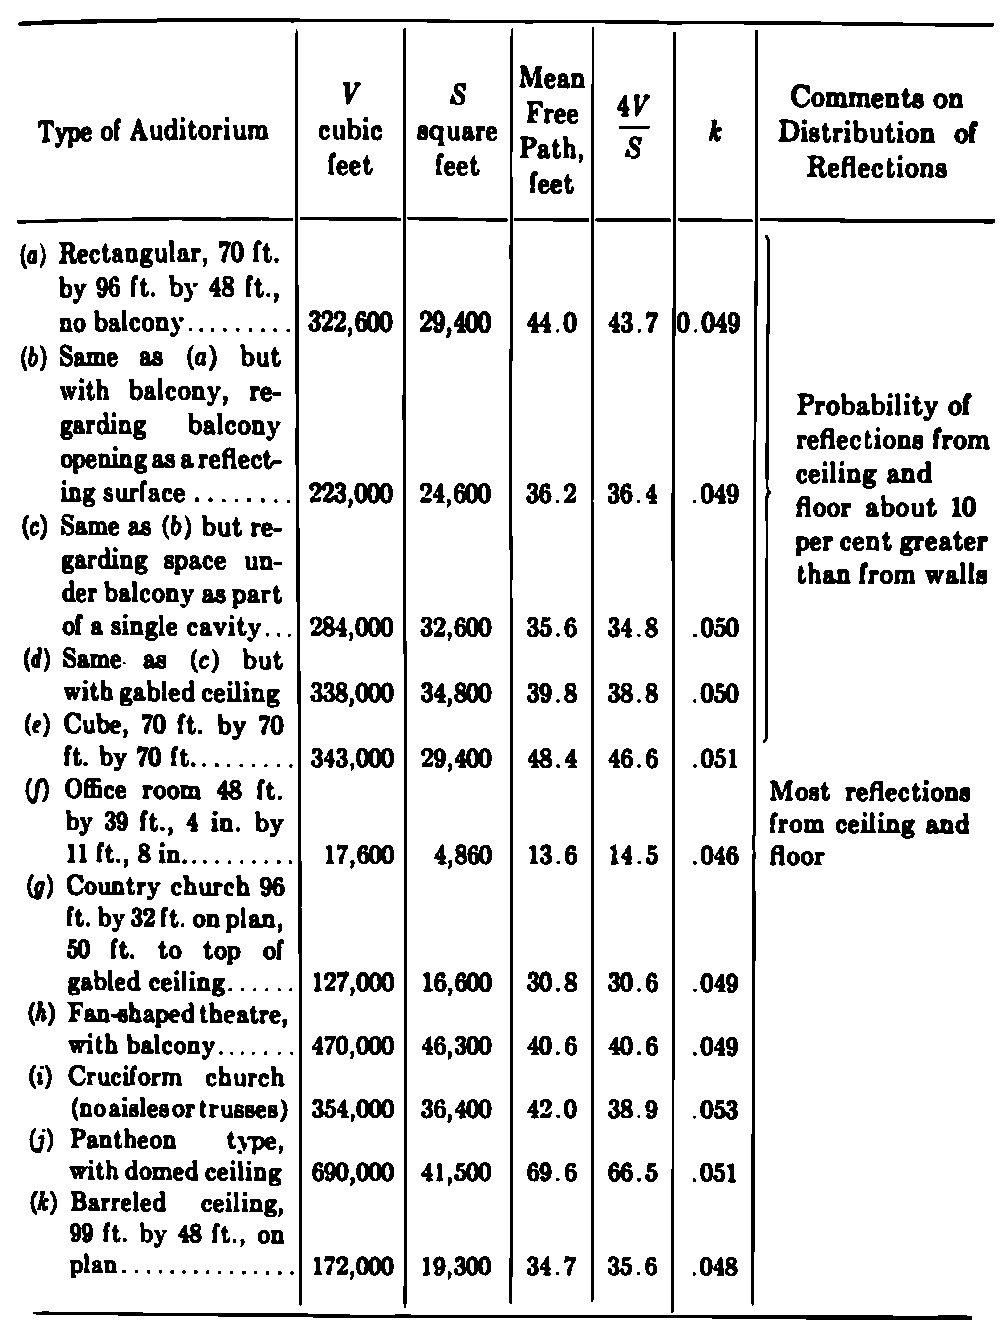
\includegraphics[width=0.9\linewidth]{archivos/mfpknudsen2.pdf}
        \caption{}
        \label{fig:knudsen2}
    \end{subfigure}
    \caption{a) Modelos utilizados para el cálculo de MFP por Vern O. Knudsen. Figura extraída del libro \cite{Knudsen1932}, pág. 140. b) Resultados obtenidos con el cálculo de MFP por Vern O. Knudsen. Tabla extraída del libro \cite{Knudsen1932}, pág. 141.}
\end{figure}
\FloatBarrier 

El factor $k$ es el valor que multiplica a $V/A$ en la ecuación del tiempo de reverberación (ecuación \ref{ecu:tr}). En la tabla (figura \ref{fig:knudsen2}) está en unidades del sistema imperial, la conversión al sistema internacional de unidades se obtiene multiplicando por la velocidad del sonido en unidades imperiales (1124 pies/s) y dividiendo por la misma velocidad en unidades métricas (343 m/s), tal que $k_\text{S.I.} = k_\text{I.}\cdot\nicefrac{1124}{343}$.

Este factor $k$ se obtiene mediante:
\begin{flalign}
	 k=l_{\mathrm{MFP}}\frac{S\ln 10^6}{ Vc}\label{factork}
\end{flalign}
\begin{condiciones}[Donde:]
	l_{\mathrm{MFP}} & \rightarrow & Es el valor de MFP experimental en metros.
\end{condiciones}


\subsection{Tiempo de reverberación}

El tiempo de reverberación se define como el tiempo que transcurre para que el nivel de presión de un sonido se reduzca 60 $dB$ (una millonésima parte) desde el instante que deja de emitirse. Siempre se expresa en segundos.

\begin{figure}[ht]
    \centering
    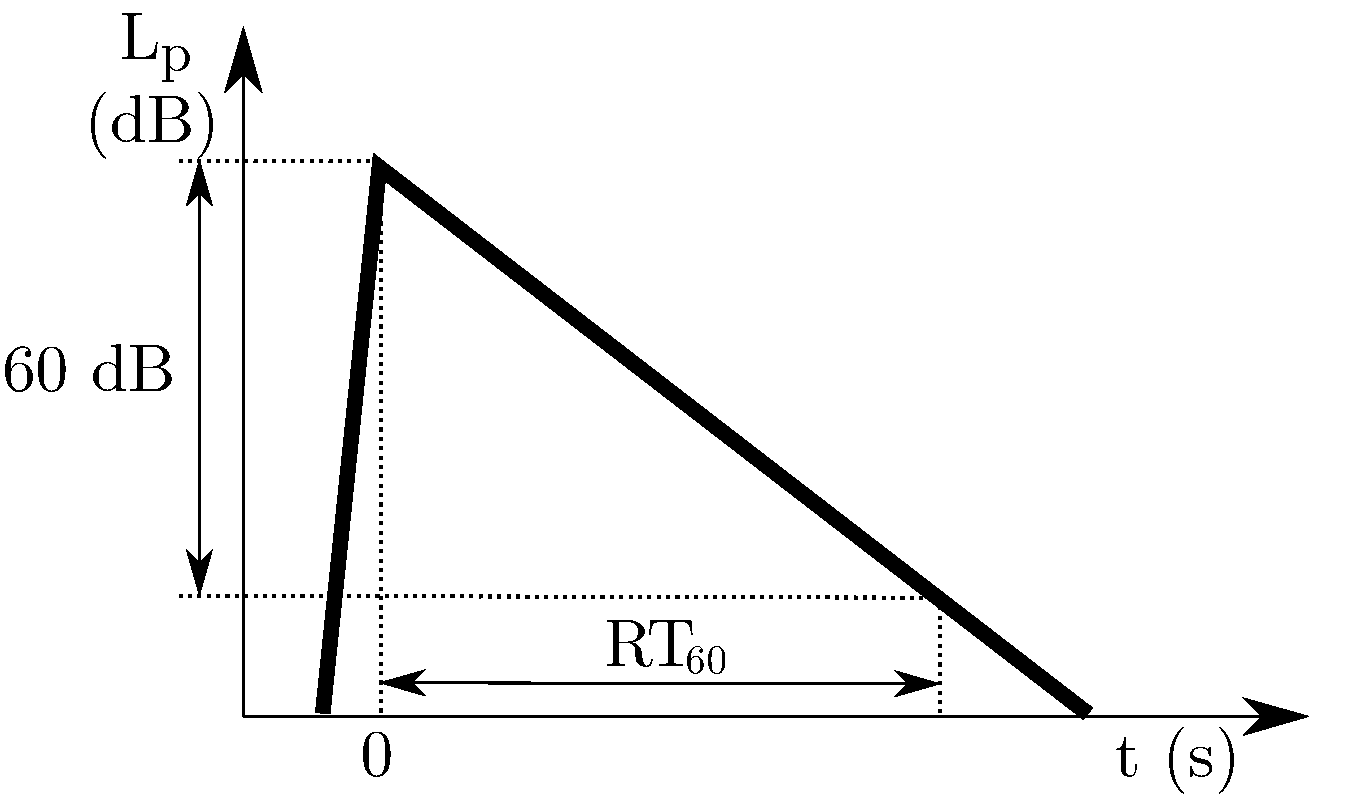
\includegraphics[width=0.4\textwidth]{archivos/tiempoRT.pdf}
    \caption{Diagrama de la definición de tiempo de reverberación.}
\end{figure}
\FloatBarrier

En la práctica es difícil medir una caída completa de 60 $dB$ por lo que es habitual utilizar:

\begin{description}
	\item [EDT:] \textit{Early Decay Time}. Es el tiempo que transcurre para que el nivel de presión se reduzca 10 $dB$ desde el instante que deja de emitirse un sonido. Tiene relación con la sensación subjetiva de la reverberación. Definido por \cite{Jordan1970}.
	\item [T20:] Es el tiempo que transcurre desde que se ha reducido 5 $dB$ hasta que se ha reducido 25 $dB$. Describe las propiedades acústicas del recinto. Definido por \cite{Atal1966}.
	\item [T30:] Es el tiempo que transcurre desde que se ha reducido 5 $dB$ hasta que se ha reducido 35 $dB$. Describe las propiedades acústicas del recinto. Definido por \cite{Atal1966}.
\end{description}

Una vez obtenido uno de estos valores se extrapola para obtener el tiempo para una caída de 60 $dB$, es decir, el EDT se multiplica por 6, el T20 por 3 y el T30 por 2. Es una práctica habitual ofrecer el valor T20 o T30 ya extrapolado.

\begin{figure}[ht]
    \centering
    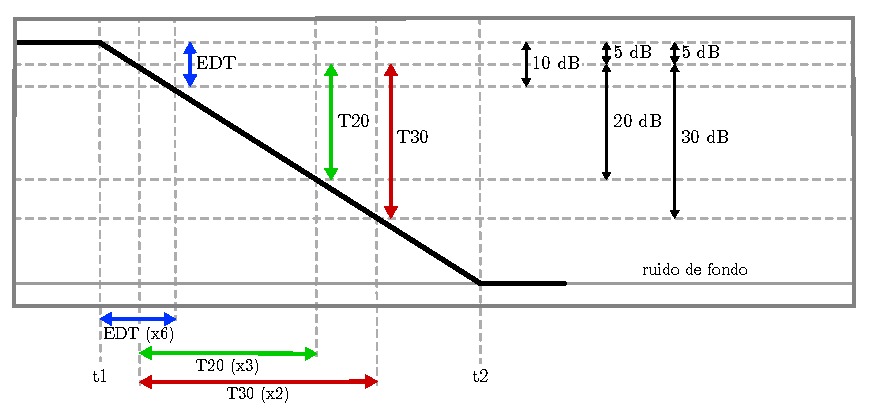
\includegraphics[width=0.8\textwidth]{archivos/EDT2030.pdf}
    \caption{Diagrama de la definición de EDT, T20 y T30.}
\end{figure}
\FloatBarrier

El cálculo teórico del tiempo de reverberación tiene en consideración la superficie, volumen y absorción del recinto. Existen en la literatura múltiples propuestas para el cálculo del tiempo de reverberación, aquí se explicarán las dos más comunes, \citeauthor{Sabine1922} y \citeauthor{Eyring1930}:

\begin{description}
	\item [Sabine:] Wallace Clement Sabine propuso su método de cálculo al final del siglo XIX que más tarde fue recogido en \textit{Collected Papers on Acoustics} \citep{Sabine1922}. Este cálculo es útil cuando el coeficiente de absorción medio $\overline{\alpha}$ se encuentra entre $0$-$0.2$ y el reparto es homogéneo, superado este valor el cálculo introduce errores mayores al 10\%.
		\begin{flalign}\label{eq:sabine}
			T = \frac{l_{\mathrm{MFP}} \ln 10^6 }{c\ \overline{\alpha}}=\frac{4 \ln 10^6\ V}{c\ S\ \overline{\alpha}}=\frac{4 \ln 10^6\ V}{c\ S\ \overline{\alpha}}\approx 0,161\frac{V}{S\ \overline{\alpha}}
		\end{flalign}
	
	\item [Eyring:] Carl Ferdinand Eyring propuso una mejora en el cálculo de \citeauthor{Sabine1922} en \cite{Eyring1930}, modificando el término de absorción total o equivalente $A$. En este caso se corrige el problema para un coeficiente mayor a $0.2$ aunque el reparto de los coeficientes debe seguir siendo homogéneo\footnote{Para un coeficiente cercano al 1 y/o  reparto de coeficientes muy extremos tanto Sabine como Eyring no son fiables, en casos como éste se debe utilizar \cite{Millington1932}.}. 
		\begin{flalign}\label{eq:eyring}
			T = \frac{l_{\mathrm{MFP}} \ln 10^6 }{-c\ \ln (1-\overline{\alpha})} = \frac{4 \ln 10^6\ V}{-c\ S \ln (1-\overline{\alpha})}\approx 0,161\frac{V}{-S \ln (1-\overline{\alpha})}
		\end{flalign}
\end{description}

Ambas ecuaciones tienen similitudes y en la literatura es habitual encontrar la ecuación del tiempo de reverberación como:
\begin{flalign}
	T =k\frac{V}{A}\approx 0,161\frac{V}{A}\label{ecu:tr}
\end{flalign}
\begin{condiciones}[Donde:]
k & \rightarrow & Constante proporcional al MFP del recinto 	(ecuación \ref{factork}).\\
A & \rightarrow & Puede ser 	$\left\{ \begin{array}{c}S\ \overline{\alpha} \quad\quad\quad\quad\;\;\; \text{Absorción equivalente de Sabine.}\\ -S \ln (1-\overline{\alpha})  \quad \text{Absorción equivalente de Eyring.}\end{array} \right.$
\end{condiciones}

\section{Parámetros de inteligibilidad y calidad acústica}

La inteligibilidad de forma genérica en la acústica se refiere a la medición de la capacidad para comprender la voz hablada. A continuación se definen algunos de los parámetros más importantes asociados a la inteligibilidad y se comentarán también algunos relacionados con la música. Existen multitud de parámetros para evaluar la inteligibilidad o la calidad acústica de un recinto, en este trabajo se exponen únicamente los desarrollados en el capítulo de resultados. Si se desea conocer muchos de estos parámetros, en \cite{Lacatis2008} se muestra un histórico de los parámetros acústicos junto a los autores y los artículos.

\subsection{Claridad C50,C80}
\label{claridad}
La claridad fue establecida por \cite{Reichardt1974} y ampliada por múltiples autores donde destaca \cite{Marshall1994}. Se define, para el caso de la palabra, como la relación entre la energía acústica recibida durante los primeros 50 milisegundos y la energía acústica después de esos 50 milisegundos, en el caso de la música el tiempo se extiende hasta los 80 milisegundos. El parámetro es adimensional y se expresa en decibelios.

Permite conocer con facilidad si predomina el campo útil sobre el campo perjudicial descritos al inicio de este capítulo. Tanto para el caso de uso para música (80 ms) como para palabra (50 ms) el cálculo general es:

\begin{flalign}
	C_t = 10\log_{10}\left( \frac{\bigints_{\;0}^{t}p^2(t)\text{d}t}{\bigints_{\;t}^{\infty}p^2(t)\text{d}t} \right)
\end{flalign}
\begin{condiciones}[Donde:]
 	t & \rightarrow & Es el periodo de integración, 50 u 80 milisegundos.\\
 	p^2 & \rightarrow & Es el valor de presión acústica al cuadrado obtenida con la respuesta al impulso (ver apartado \ref{respimpulso}).
\end{condiciones}

Este cálculo se realiza únicamente con los valores obtenidos en las bandas de octava desde 125 Hz hasta la de 4000 Hz. El valor recomendado (ISO 3382-1) para C50 debe estar comprendido entre -4dB y 4dB y para C80 entre -5dB y 5dB.
\\
\par
Además de este cálculo general es habitual el uso de los \textit{promedio} (\textit{average}). 

El C50 \textit{speech average}, definido por \cite{Marshall1994}, tiene en cuenta las bandas de octava de 500 Hz, 1000 Hz, 2000 Hz y 4000 Hz, y además incorpora una ponderación para cada una de ellas, quedando el cálculo del siguiente modo:

\begin{flalign}
	C_{50,\text{AV}} = 0.15\cdot C_{50,\text{500 Hz}} +0.25\cdot C_{50,\text{1 kHz}} + 0.35\cdot C_{50,\text{2 kHz}} + 0.25\cdot C_{50,\text{4 kHz}}
\end{flalign}

El valor recomendado para el C50 \textit{speak average} según \cite{Carrión1998} debe ser mayor a 2dB.
\\
\par 
El C80 \textit{music average} o C80(3), definido también en \cite{Marshall1994}, realiza el promedio del valor de claridad para las bandas de 500 Hz, 1000 Hz y 2000 Hz:

\begin{flalign}
	C_{80,\text{AV}} = \frac{C_{80,\text{500 Hz}}+C_{80,\text{1 kHz}}+C_{80,\text{2 kHz}}}{3}
\end{flalign}

El valor recomendado de C80(3) según \cite{beranek1986acoustics} debe estar comprendido entre -4dB y 0dB.
\\
Es posible obtener el parámetro de claridad a partir del de definición (apartado \ref{definicion}):

\begin{flalign}
	C_t = 10\log_{10}\left( \frac{D_t}{1-D_t}\right)
\end{flalign}

\subsection{Definición D50,D80}
\label{definicion}

El parámetro definición se estableció en \cite{Thiele1953}. Es similar a la claridad pero en lugar de relacionar los primeros 50 u 80 milisegundos con el resto del tiempo, se relacionan esos primeros milisegundos con el total. Del mismo modo que la claridad se tienen en cuenta las bandas de octava entre 125 Hz y 4000 Hz. 

Este parámetro es adimensional y no tiene unidades.
\vspace{-0.2cm}
\begin{flalign}
	D_t = \frac{\bigints_{\;0}^{t}p^2(t)\text{d}t}{\bigints_{\;0}^{\infty}p^2(t)\text{d}t}
\end{flalign}
\begin{condiciones}[Donde:]
 	t & \rightarrow & Es el periodo de integración, 50 u 80 milisegundos.\\
 	p^2 & \rightarrow & Es el valor de presión acústica al cuadrado obtenida con la respuesta al impulso (ver apartado \ref{respimpulso}).
\end{condiciones}

Este parámetro se puede obtener a través de la claridad operando:
\vspace{-0.2cm}
\begin{flalign}
	D_t = \frac{1}{1+10^{-\nicefrac{C_t}{10}}}
\end{flalign}

Para el D50, \cite{Arau1999} recomienda valores superiores a 0.5. En el caso del D80, dado que casi no es utilizado no hay fuentes en la literatura que recomienden valores, pero utilizando los valores de claridad C80 recomendados en la ISO 3382-1 se obtienen los valores de definición comprendidos entre 0.25 y 0.75.

\subsection{Sonoridad G}
\label{sonoridad}
La sonoridad definida en \cite{Lehmann1976} es el cociente entre el nivel recibido en un punto debido a una fuente sonora omnidireccional y el nivel que genera la misma fuente a 10 metros en campo libre. Este cálculo ofrece información sobre la ganancia acústica que produce un recinto mediante reflexiones y está inversamente relacionado con la absorción acústica del recinto. El parámetro $G$ (\textit{sound strength}) es adimensional y se expresa en escala logarítmica.

Generalmente este parámetro es utilizado en recintos para música. El cálculo tiene mayor utilidad si el recinto es lo suficientemente grande como para que la distancia entre el escenario o punto de emisión y la zona de recepción más cercana sea mayor a 10 metros. 

Este párametro se calcula como:
	\vspace{-0.2cm}
	\begin{flalign}
		G = 10\log_{10}\left( \frac{\bigints_{\;0}^{\infty} p^2(t) \text{d}t}{\bigints_{\;0}^{\infty} p^2_{10m}(t) \text{d}t} \right)= L_p - L_{p,10m}
	\end{flalign} 

En \cite{Beranek2011} se recomienda un valor entre 4 dB y 7.5 dB para la $G_{mid}$ que se refiere al parámetro $G$ teniendo en cuenta únicamente las bandas de frecuencia de 500 Hz y 1000 Hz. 



\subsection{Índice de articulación AI}
\label{indicearticulacion}
El índice de articulación es una herramienta que permite conocer la cantidad de habla que puede percibir un receptor, definido por \cite{French1947} y ampliamente desarrollado por \cite{Kryter1962}, asignando unos pesos a cada banda de frecuencia de la relación señal ruido recibida. Estos pesos están definidos por \citeauthor{Kryter1962} para tercios de octava, bandas de octava y bandas de octava habituales (de 250 Hz a 4000 Hz), aquí se va a definir el cálculo para el caso de bandas de octava habituales:

\begin{flalign}
	AI = \sum\limits_{i=1}^{5} W_iR_i
\end{flalign}

\begin{condiciones}[Donde:]
	i & \rightarrow & Es el índice de la banda de octava (250 Hz, 500 Hz, 1 kHz, 2 kHz y 4 kHz).\\
	W_i & \rightarrow & Es el peso para cada banda de frecuencia, indicado en la tabla \ref{pesosai}.\\
	R_i & \rightarrow & Es la relación señal ruido para cada banda de frecuencia en dB.
\end{condiciones}

\begin{table}[ht]
\centering
{\scalefont{0.9}
\begin{tabular}{@{}lccccc@{}}
\toprule
Frecuencia (Hz) & 250 & 500 & 1000 & 2000 & 4000 \\ \midrule
Peso $W$ & 0.0018 & 0.0050 & 0.0075 & 0.0107 & 0.0083 \\ \bottomrule
\end{tabular}
}
\caption{Peso de cada banda de octava para el cálculo de AI.}
\label{pesosai}
\end{table}
\FloatBarrier

El valor comprende entre 0 y 1, donde 0 es el valor correspondiente al nulo entendimiento del habla y 1 al completo entendimiento de éste.

\citeauthor{Kryter1962} también define una corrección del AI debido al tiempo de reverberación del recinto representado por la curva de la figura \ref{graf:correcionai}.

\begin{figure}[ht]
    \centering
    {\scalefont{0.8}
    %%%%%%%%%%%%%%%%%%%%%%%%%%%%%%%%%%%%%%%%%%%%%%%%%%%%%%%%%%%%%%%%%%%%%%%%
% Escuela Politécnica Superior de la Universidad de Alicante
% Realizado por: Jose Manuel Requena Plens
% Contacto: info@jmrplens.com / Telegram:@jmrplens
%%%%%%%%%%%%%%%%%%%%%%%%%%%%%%%%%%%%%%%%%%%%%%%%%%%%%%%%%%%%%%%%%%%%%%%%

\definecolor{mycolor1}{rgb}{0.00000,0.44700,0.74100}%
%
\begin{tikzpicture}

\begin{axis}[%
width=0.5\textwidth,
height=0.3\textwidth,
at={(0\textwidth,0\textwidth)},
scale only axis,
xmin=0,
xmax=10,
xlabel style={font=\color{white!15!black}},
xlabel={Tiempo de reverberación (s)},
xtick distance=1,
minor x tick num= 1,
minor y tick num= 1,
ymin=0,
ymax=1,
ytick distance=0.1,
grid=both,
ylabel style={font=\color{white!15!black}},
ylabel={Reducción de AI},
axis background/.style={fill=white},
legend style={legend cell align=left, align=left, draw=white!15!black}
]

\addplot[color=black,line width=2.0pt,domain=0:10, samples=85]{0.0004264*x^4 -0.008245*x^3 + 0.04282*x^2 + 0.06021*x + 0.007629};
\end{axis}
\end{tikzpicture}%
    }
    \caption{Valores de corrección de AI según tiempo de reverberación.}
    \label{graf:correcionai}
\end{figure}
\FloatBarrier

Este parámetro da pie a crear un índice buscando el efecto contrario, zonas donde la privacidad de la conversación sea máxima, este índice de privacidad se calcula como:
\begin{flalign}
	PI = 1 - AI
\end{flalign}

Teniendo privacidad máxima con un índice igual a 0, y ninguna privacidad con un valor igual a 1.

\section{Teoría de campos acústicos}

La teoría de los campos acústicos aplicada en este trabajo es la desarrollada en el apartado \ref{teoriarevisadacorregida}, denominada \textit{teoría revisada corregida}. A continuación se muestran los antecedentes del cálculo de los campos acústicos.

\subsection{Campos directo y reverberado}

El campo directo por definición es el campo generado por las ondas sonoras que no han sufrido reflexiones, mientras que el campo reverberado es el campo generado por las ondas sonoras que han sufrido al menos una reflexión. Habitualmente el campo reverberado se descompone en campo temprano y campo tardío (\textit{early field} y \textit{late field}). También se puede denominar reflexión temprana y tardía o primeras reflexiones y cola reverberante.

%\begin{figure}[ht]
%    \centering
%    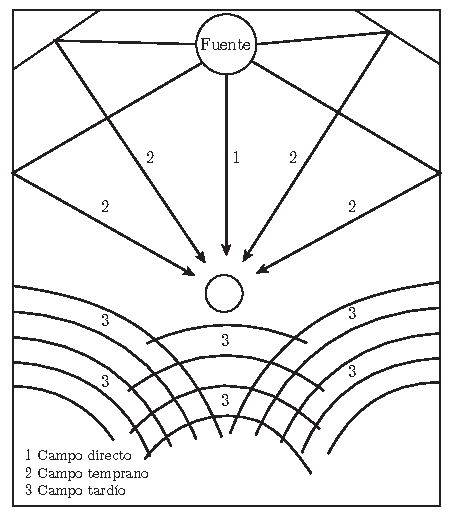
\includegraphics[width=0.4\textwidth]{archivos/campos.pdf}
%    \caption{Descripción de los campos acústicos. Figura extraída y modificada de \cite{Self2009}, pág. 111.}
%    \label{descampos}
%\end{figure}
\begin{figure}[ht]
    \centering
    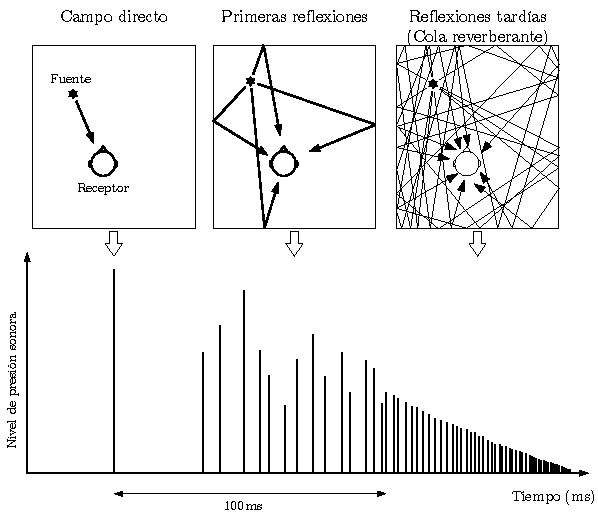
\includegraphics[width=0.65\textwidth]{archivos/campos2.pdf}
    \caption{Ecograma asociado a un receptor con indicación del campo directo, las primeras reflexiones y la cola reverberante. Figura extraída de \cite{Carrión1998}, pág. 50.}
    \label{ecograma}
\end{figure}
Un ecograma (figura \ref{ecograma}) muestra el nivel y tiempo de llegada de cada rayo sonoro a un receptor, facilitando la representación de los campos acústicos en el receptor.
En la práctica es relativamente sencillo desglosar la historia temporal (campo directo, primeras reflexiones y cola reverberante), se suele separar la pendiente en $\Delta t$ para separar el campo en un símil de rayos acústicos. Habitualmente se separa en incrementos de 1 milisegundo.

\par Para el cálculo teórico se ha escrito mucho pero existe una teoría sobradamente aceptada; es la propuesta de \cite{Hopkins1948} que describe el campo acústico total como la suma del campo directo y el campo reverberado, que años más tarde fue modificada por \cite{davis1984}. Este cálculo asume que el campo reverberante es estacionario, es decir, constante en cualquier punto del recinto.

\begin{flalign}
	I =& \frac{WQ}{4\pi r^2} + \frac{4W}{A}\label{eq:hopkins}
\end{flalign}
\begin{condiciones}[Donde:]
	I & \rightarrow & Es la intensidad acústica total en $W/m^2$.\\
	r & \rightarrow & Es la distancia emisor-receptor en metros.\\
	A & \rightarrow & Es la absorción equivalente de Sabine o Eyring.
\end{condiciones}

El término $\nicefrac{WQ}{4\pi r^2}$ corresponde a la intensidad del campo directo a distancia $r$ de la fuente y el término $\nicefrac{4W}{A}$ corresponde a la intensidad del campo reverberado que, como se puede observar, presupone que es constante en cualquier punto del recinto.

\begin{figure}[ht]
    \centering
    {\scalefont{0.8}
    %%%%%%%%%%%%%%%%%%%%%%%%%%%%%%%%%%%%%%%%%%%%%%%%%%%%%%%%%%%%%%%%%%%%%%%%
% Escuela Politécnica Superior de la Universidad de Alicante
% Realizado por: Jose Manuel Requena Plens
% Contacto: info@jmrplens.com / Telegram:@jmrplens
%%%%%%%%%%%%%%%%%%%%%%%%%%%%%%%%%%%%%%%%%%%%%%%%%%%%%%%%%%%%%%%%%%%%%%%%

\definecolor{mycolor1}{rgb}{0.60000,0.00000,0.60000}%
%
\begin{tikzpicture}

\begin{axis}[%
width=0.5\textwidth,
height=0.3\textwidth,
at={(0\textwidth,0\textwidth)},
scale only axis,
xmin=0,
xmax=10,
xlabel style={font=\color{white!15!black}},
xlabel={Distancia (m)},
ymin=75,
ymax=100,
ytick distance=5,
ylabel style={font=\color{white!15!black}},
ylabel={Nivel de presión acústica (dB)},
axis background/.style={fill=white},
xmajorgrids,
ymajorgrids,
legend style={at={(0.5,-0.03)}, anchor=north, legend cell align=left, align=left, draw=white!15!black},
legend columns = 2,legend style={at={(0.5,-0.2)}, anchor=north, legend cell align=left, align=left, draw=white!70!black, /tikz/every even column/.append style={column sep=1.0cm}}
]
\addplot [color=blue,line width=1.5pt]
  table[row sep=crcr]{%
0.911043357914437	97.6380061935451\\
0.971043357914425	97.0416130715755\\
1.03104335791443	96.484310473315\\
1.10104335791443	95.8774048250365\\
1.17104335791443	95.3113917575971\\
1.24104335791444	94.7813060660669\\
1.31104335791443	94.2830244776188\\
1.38104335791444	93.8130865478216\\
1.46104335791443	93.3069806543866\\
1.54104335791443	92.8303775474136\\
1.62104335791443	92.3801537924959\\
1.70104335791443	91.9536509875259\\
1.78104335791443	91.5485883526324\\
1.87104335791443	91.1160767261982\\
1.96104335791443	90.7057903345106\\
2.05104335791444	90.3156426154386\\
2.14104335791443	89.9438239896602\\
2.23104335791443	89.5887552104351\\
2.33104335791442	89.2121989170647\\
2.43104335791443	88.8529466109456\\
2.53104335791443	88.5095386461936\\
2.63104335791444	88.1806902279387\\
2.74104335791444	87.8344205548337\\
2.85104335791443	87.5030577659302\\
2.96104335791443	87.1854208783258\\
3.07104335791443	86.8804620884833\\
3.18104335791443	86.5872475992273\\
3.30104335791444	86.2797919676868\\
3.42104335791443	85.9843498413856\\
3.54104335791443	85.7000543544441\\
3.66104335791444	85.426127966722\\
3.79104335791443	85.1402654198586\\
3.92104335791443	84.8649508844128\\
4.05104335791444	84.5994642356986\\
4.18104335791443	84.3431556826281\\
4.32104335791443	84.0767218124595\\
4.46104335791443	83.8195859804349\\
4.60104335791443	83.5711467621151\\
4.75104335791443	83.3139935284142\\
4.90104335791443	83.0655890600581\\
5.05104335791444	82.8253812483105\\
5.20104335791443	82.5928679479935\\
5.36104335791443	82.3528195444158\\
5.52104335791444	82.120498287441\\
5.68104335791443	81.8954420472253\\
5.85104335791443	81.6638082159739\\
6.02104335791444	81.4394362677818\\
6.19104335791442	81.2219029078978\\
6.37104335791443	80.9985968064552\\
6.55104335791444	80.7821012050116\\
6.74104335791444	80.5605400646246\\
6.93104335791443	80.3457203545647\\
7.12104335791443	80.1372603842554\\
7.32104335791443	79.9243144622446\\
7.52104335791444	79.7176514144308\\
7.73104335791443	79.5070397973059\\
7.94104335791442	79.3026073677421\\
8.15104335791443	79.1040164504568\\
8.37104335791443	78.9018955433603\\
8.59104335791443	78.7055148221739\\
8.82104335791443	78.5060156380693\\
9.05104335791444	78.3121381646318\\
9.14104335791443	78.2377385102596\\
};
\addlegendentry{Campo directo - Experimental}

\addplot [color=red,line width=1.5pt]
  table[row sep=crcr]{%
0.911043357914437	97.5218752230605\\
9.14104335791443	94.9864450736265\\
};
\addlegendentry{Campo reverberante - Experimental}

\addplot [color=black, densely dotted, line width=1.5pt]
  table[row sep=crcr]{%
0.911043357914437	97.7331926631792\\
0.971043357914425	97.1792011477379\\
1.04104335791443	96.5745972347531\\
1.11104335791443	96.0093534389856\\
1.18104335791443	95.4786567564759\\
1.25104335791443	94.9785263574731\\
1.33104335791442	94.4401295353534\\
1.41104335791444	93.9331664115882\\
1.49104335791444	93.4541681380115\\
1.57104335791443	93.0002101682137\\
1.65104335791443	92.5688040192524\\
1.74104335791444	92.1077818536397\\
1.83104335791442	91.67000102226\\
1.92104335791443	91.253230247119\\
2.01104335791443	90.8555449059847\\
2.11104335791443	90.4340305227801\\
2.21104335791443	90.0320284059368\\
2.31104335791443	89.6478117182375\\
2.41104335791444	89.2798731791945\\
2.52104335791444	88.892367288714\\
2.63104335791444	88.5214134861318\\
2.74104335791444	88.1656554813739\\
2.85104335791443	87.8238971470306\\
2.97104335791443	87.4657937924312\\
3.09104335791443	87.121871648269\\
3.21104335791443	86.7910501914252\\
3.33104335791442	86.4723678740925\\
3.46104335791443	86.1398327886619\\
3.59104335791443	85.8195606111837\\
3.72104335791443	85.5106789771931\\
3.85104335791443	85.2124054217199\\
3.99104335791444	84.9022446689407\\
4.13104335791444	84.602778523021\\
4.27104335791444	84.3132939822976\\
4.41104335791444	84.033147053859\\
4.56104335791443	83.7426895724501\\
4.71104335791443	83.4616315615413\\
4.86104335791443	83.1893836916001\\
5.02104335791444	82.9080941543875\\
5.18104335791443	82.635629052434\\
5.34104335791443	82.3714515163175\\
5.51104335791443	82.0992970302704\\
5.68104335791443	81.8354115101393\\
5.85104335791443	81.5793072595462\\
6.03104335791443	81.3161245733647\\
6.21104335791443	81.0606823675505\\
6.39104335791443	80.8125383092309\\
6.58104335791442	80.5580785454699\\
6.77104335791444	80.3108616913113\\
6.96104335791443	80.0704868101745\\
7.16104335791444	79.8244475218628\\
7.36104335791443	79.585186070651\\
7.57104335791443	79.3408589206871\\
7.78104335791443	79.1032168805553\\
7.99104335791444	78.8719038454604\\
8.21104335791443	78.6360066789118\\
8.43104335791443	78.4063471322951\\
8.66104335791444	78.1725693325264\\
8.89104335791443	77.9449190244605\\
9.13104335791444	77.7135654870847\\
9.14104335791443	77.704058208972\\
};
\addlegendentry{Campo directo - Hopkins-Stryker}

\addplot [color=black, dashed, line width=1.5pt]
  table[row sep=crcr]{%
0.911043357914437	96.7131831634935\\
9.14104335791443	96.7131831634935\\
};
\addlegendentry{Campo reverberante - Hopkins-Stryker}



\end{axis}
\end{tikzpicture}%
    }
    \caption{Comparación de los campos acústicos obtenidos experimentalmente y mediante la ecuación Hopkins-Stryker. El tiempo de integración del experimental es 0-1 ms para el campo directo y 1-$\infty$ para el campo reverberante.}
    \label{graf:hopkinsstryker}
\end{figure}

Se ha comprobado empíricamente que el término de campo directo corresponde aproximadamente al espacio temporal de 0 a 1ms\footnote{Esta afirmación es válida cuando los datos son ideales temporalmente hablando, tal como los ofrece un programa de simulación acústica, en la práctica el espacio temporal del campo directo fluctúa entre los 2 y los 10 milisegundos.\label{unmilisegundo}} de un ecograma y el término del campo reverberado corresponde aproximadamente al espacio temporal desde 1ms a infinito (figura \ref{graf:hopkinsstryker}). 

\subsubsection{Distancia crítica}

La distancia crítica se define como la distancia donde el campo directo y el reverberado se cruzan, a partir de este punto el campo reverberante predomina sobre el campo directo y se indica como una zona de baja inteligibilidad. Esto no es correcto, estando comprobado empíricamente que esta distancia no se aproxima a la zona donde la inteligibilidad se reduce.

El cálculo de la distancia crítica es una función derivada de la ecuación Hopkins-Stryker \ref{eq:hopkins}, se puede obtener fácilmente igualando los términos de ambos campos y despejando la distancia, así se obtiene la distancia donde el valor de los campos es el mismo.

\begin{flalign*}
	&& \frac{WQ}{4\pi D_c^2} &= \frac{4W}{A} &&\\
	&& \frac{Q}{4\pi D_c^2} &= \frac{4}{A} &&
\end{flalign*}
\begin{flalign}
	D_c = \sqrt{\frac{QA}{16\pi}}
\end{flalign}
\begin{condiciones}[Donde:]
	D_c & \rightarrow & Es la distancia crítica en metros.\\
	A & \rightarrow & Es la absorción equivalente de Sabine o Eyring.
\end{condiciones}

\subsection{Teoría revisada o moderna}
\label{teoriarevisada}

La \textit{teoría revisada} o \textit{teoría moderna} es una mejora del cálculo de campos acústicos propuesta por \cite{Barron1988} y ampliada en \cite{Barron2015}, en la que se describe mejor el comportamiento de los mismos. En esta \textit{teoría revisada} el campo reverberante ya no se considera estacionario o constante sino que tiene una pendiente respecto a la distancia, además permite obtener los campos acústicos definiendo un tiempo de integración para los diferentes campos.

El campo total se calcula como:
\begin{flalign*}
	I_0^\infty (r,t)&= \frac{WQ}{4\pi r^2} + \frac{4W}{A} 10^{-\left(\frac{60t}{10T} \right)}\\
	I_0^\infty (r,t)&= \frac{WQ}{4\pi r^2} + \frac{4W}{A} e^{-\left(\frac{6\ln(10)t}{T} \right)}\\
\end{flalign*}
\vspace{-1cm}
\begin{flalign}
	I_0^\infty (r,t)&= \frac{WQ}{4\pi r^2} + \frac{4W}{A} e^{-\left(\frac{13,82t}{T} \right)}\label{eq:barronT}
\end{flalign}
\begin{condiciones}[Donde:]
	I_0^\infty & \rightarrow & Es la intensidad acústica total en $W/m^2$. Desde 0 milisegundos a infinito (fin de la cola reverberante).\\
	r & \rightarrow & Es la distancia emisor-receptor en metros.\\
	t & \rightarrow & Es el tiempo que tarda el sonido desde el emisor al receptor en segundos.\\
	T & \rightarrow & Es el tiempo de reverberación.\\
	A & \rightarrow & Es la absorción equivalente de Sabine o Eyring.
\end{condiciones}
El tiempo $t$ se puede sustituir por $r/c$ para que en lugar de estar en función del tiempo y la distancia se calcule sólo en función de la distancia emisor-receptor ($r=$ distancia ; $c=$ velocidad del sonido en el aire).


La ecuación permite obtener el campo de primeras reflexiones y el de cola reverberante por separado a partir del término de campo reverberante incluido en la ecuación \ref{eq:barronT} (segundo sumando). Con ello es posible redefinir los campos como \textit{campo útil} (0 - $t_0$) y \textit{campo perjudicial} ($t_0$ - $\infty$). El campo útil incluye el campo directo y el campo temprano; y el campo perjudicial el campo reverberante. Para obtener el campo temprano se realiza la diferencia entre el total del campo reverberante (segundo sumando de la ecuación anterior) y el campo a partir de cierto tiempo de integración (campo reverberante), obteniendo así el campo entre 1 milisegundo y $t_0$ también denominado temprano o \textit{early}. 


\begin{flalign}
	I_L = I_t^\infty (r)&= \frac{4W}{A} e^{-\left(\frac{13,82\left(\frac{r}{c}+t_0\right)}{T}\right)}\\
	I_E = I_1^t (r)&= \frac{4W}{A} \left(e^{-\left(\frac{13,82\frac{r}{c}}{T}\right)} - e^{-\left(\frac{13,82\left(\frac{r}{c}+t_0\right)}{T}\right)}\right)\label{tempranobarron}
\end{flalign}
\begin{condiciones}[Donde:]
	I_t^\infty & \rightarrow & Es la intensidad del campo tardío o cola reverberante (\textit{Late}) en $W/m^2$ desde el tiempo $t_0$ a infinito. Este campo pasa a denominarse \textit{campo perjudicial}.\\
	I_1^t & \rightarrow & Es la intensidad del campo temprano o primeras reflexiones (\textit{Early}) en $W/m^2$ desde 1 ms a $t_0$. No tiene en cuenta el campo directo que ocupa el espacio temporal de 0 a 1 milisegundo\textsuperscript{\ref{unmilisegundo}}.\\
	t_0 & \rightarrow & Es el tiempo de integración, en segundos, donde terminan las primeras reflexiones y comienza la cola reverberante. En recintos para palabra el tiempo son 50 milisegundos y para música 80 milisegundos \citep{Haas1949}.
\end{condiciones}

Por lo que el cálculo general de la teoría revisada para el campo útil y el campo perjudicial se calculan como:

\begin{flalign}
	I_t^\infty (r)&= \frac{4W}{A} e^{-\left(\frac{13,82\left(\frac{r}{c}+t_0\right)}{T}\right)}\\
	I_0^t (r)&= \frac{WQ}{4\pi r^2} + \frac{4W}{A} \left(e^{-\left(\frac{13,82\frac{r}{c}}{T}\right)} - e^{-\left(\frac{13,82\left(\frac{r}{c}+t_0\right)}{T}\right)}\right)
\end{flalign}
\begin{condiciones}[Donde:]
	I_0^t & \rightarrow & Es la intensidad del campo útil en $W/m^2$ para el tiempo de integración de 0 a $t_0$.\\
	I_t^\infty & \rightarrow & Es la intensidad del campo perjudicial en $W/m^2$ para el tiempo de integración de $t_0$ a infinito.
\end{condiciones}


También es posible obtener directamente el nivel de presión acústica teniendo en cuenta la ecuación \ref{eq:intensidadimpedancia} y \ref{eq:nivelpresion}:

\begin{flalign}
	L_p{_t^\infty} (r)&= 10\log_{10} \left[\frac{Z}{p_0^2} \left(\frac{4W}{A} e^{-\left(\frac{13,82\left(\frac{r}{c}+t_0\right)}{T}\right)}\right)\right]\label{eq:barron1}\\
	L_p{_0^t} (r)&= 10\log_{10} \left[\frac{Z}{p_0^2} \left(\frac{WQ}{4\pi r^2} +\frac{4W}{A} \left(e^{-\left(\frac{13,82\frac{r}{c}}{T}\right)} -e^{-\left(\frac{13,82\left(\frac{r}{c}+t_0\right)}{T}\right)}\right)\right)\right]\label{eq:barron2}
\end{flalign}

Como curiosidad, \cite{Barron1988} proponen introducir la potencia acústica en picovatios ($10^{-12}$), con ello el término $Z/p_o^2 \approx 10^{12}$ se anula. Esta simplificación introduce una pérdida aproximada del 3\% de intensidad acústica, por lo que la simplificación no se utilizará.

Se ha comparado la \textit{teoría revisada} de \cite{Barron1988} con los resultados obtenidos experimentalmente (figura \ref{graf:barron}) y siguen sin ajustarse al comportamiento real de un recinto; las pendientes son similares pero los niveles absolutos no se ajustan, por lo que el punto de cruce o distancia crítica obtenida con la \textit{teoría revisada} no es correcta.

\begin{figure}[ht]
    \centering
    {\scalefont{0.8}
    %%%%%%%%%%%%%%%%%%%%%%%%%%%%%%%%%%%%%%%%%%%%%%%%%%%%%%%%%%%%%%%%%%%%%%%%
% Escuela Politécnica Superior de la Universidad de Alicante
% Realizado por: Jose Manuel Requena Plens
% Contacto: info@jmrplens.com / Telegram:@jmrplens
%%%%%%%%%%%%%%%%%%%%%%%%%%%%%%%%%%%%%%%%%%%%%%%%%%%%%%%%%%%%%%%%%%%%%%%%

\definecolor{mycolor1}{rgb}{0.60000,0.00000,0.60000}%
%
\begin{tikzpicture}

\begin{axis}[%
width=0.5\textwidth,
height=0.4\textwidth,
at={(0\textwidth,0\textwidth)},
scale only axis,
xmin=0,
xmax=10,
xlabel style={font=\color{white!15!black}},
xlabel={Distancia (m)},
ymin=90,
ymax=100,
ylabel style={font=\color{white!15!black}},
ylabel={Nivel de presión acústica (dB)},
axis background/.style={fill=white},
xmajorgrids,
ymajorgrids,
legend style={at={(0.5,-0.03)}, anchor=north, legend cell align=left, align=left, draw=white!15!black},
legend columns = 2,legend style={at={(0.5,-0.2)}, anchor=north, legend cell align=left, align=left, draw=white!70!black, /tikz/every even column/.append style={column sep=1.0cm}}
]

\addplot [color=blue,line width=1.5pt]
  table[row sep=crcr]{%
0.911043357914437	99.0320903003883\\
0.971043357914425	98.7959528580098\\
1.04104335791443	98.5388845359429\\
1.11104335791443	98.2991565611425\\
1.18104335791443	98.0746113747233\\
1.25104335791443	97.8634686967113\\
1.33104335791442	97.6366789189634\\
1.41104335791444	97.4236104651384\\
1.49104335791444	97.2227224106986\\
1.57104335791443	97.0327183901271\\
1.66104335791444	96.8306093715308\\
1.75104335791443	96.6395556707976\\
1.84104335791443	96.4584289152229\\
1.93104335791443	96.2862642660283\\
2.03104335791443	96.1044739711391\\
2.13104335791444	95.9317415415692\\
2.23104335791443	95.7672211044658\\
2.34104335791443	95.5948612142661\\
2.45104335791443	95.4307062204238\\
2.56104335791443	95.2740225949879\\
2.68104335791443	95.1108663553771\\
2.80104335791444	94.9551165840878\\
2.92104335791443	94.806140571678\\
3.05104335791444	94.6517513929231\\
3.18104335791443	94.5040410792525\\
3.32104335791443	94.3518142639458\\
3.46104335791443	94.2061042231499\\
3.60104335791443	94.0663847075716\\
3.75104335791443	93.9228053201509\\
3.90104335791443	93.7850628689417\\
4.06104335791443	93.6440668175321\\
4.22104335791443	93.5087197458185\\
4.39104335791443	93.3706251877107\\
4.56104335791443	93.237969212078\\
4.74104335791444	93.1029881074567\\
4.92104335791443	92.9732220826459\\
5.11104335791443	92.8414835983793\\
5.31104335791443	92.7081906576988\\
5.51104335791443	92.5800064516834\\
5.72104335791443	92.4505060443611\\
5.94104335791442	92.3200245358077\\
6.16104335791444	92.194462292896\\
6.39104335791443	92.0680713703988\\
6.63104335791444	91.9411199156829\\
6.88104335791444	91.8138503478675\\
7.14104335791443	91.6864807854776\\
7.40104335791443	91.5638340591942\\
7.67104335791443	91.4411133083876\\
7.95104335791443	91.3184925375982\\
8.24104335791444	91.196127426742\\
8.54104335791443	91.0741566576816\\
8.85104335791443	90.9527032209901\\
9.14104335791443	90.8430159904712\\
};
\addlegendentry{Campo útil - Experimental}

\addplot [color=red,line width=1.5pt]
  table[row sep=crcr]{%
0.911043357914437	94.3187674098585\\
9.14104335791443	93.1435779651411\\
};
\addlegendentry{Campo perjudicial - Experimental}

\addplot [color=black, densely dotted, line width=1.5pt]
  table[row sep=crcr]{%
0.911043357914437	98.8442038515845\\
0.961043357914434	98.4878235681649\\
1.01104335791443	98.1576951001293\\
1.07104335791443	97.7926079050455\\
1.13104335791444	97.4578325100523\\
1.19104335791442	97.1501002865041\\
1.25104335791443	96.8665894754342\\
1.31104335791443	96.6048471671477\\
1.37104335791443	96.3627282942134\\
1.43104335791443	96.1383472350854\\
1.49104335791444	95.9300389116959\\
1.55104335791442	95.7363271398722\\
1.61104335791443	95.555898597231\\
1.67104335791443	95.3875811986474\\
1.73104335791443	95.23032597233\\
1.80104335791442	95.0595926546016\\
1.87104335791443	94.901305889186\\
1.94104335791442	94.7542844690337\\
2.01104335791443	94.6174790500056\\
2.08104335791442	94.4899551720248\\
2.15104335791443	94.3708788045371\\
2.22104335791443	94.259503977668\\
2.30104335791444	94.1407945073161\\
2.38104335791444	94.0303835636486\\
2.46104335791443	93.9274826267694\\
2.54104335791443	93.8313912722203\\
2.62104335791443	93.741485979835\\
2.71104335791443	93.6470465944395\\
2.80104335791444	93.5590307995579\\
2.89104335791443	93.4768171561182\\
2.99104335791444	93.391606367548\\
3.09104335791443	93.3122145729496\\
3.19104335791442	93.2380566026667\\
3.30104335791444	93.1619146157453\\
3.41104335791444	93.090880868525\\
3.53104335791443	93.0185980984089\\
3.65104335791443	92.9511719041935\\
3.78104335791443	92.8830069298233\\
3.92104335791443	92.8146372138352\\
4.07104335791443	92.7465020593473\\
4.22104335791443	92.683028919034\\
4.38104335791444	92.6198398689944\\
4.55104335791444	92.5571826645204\\
4.74104335791444	92.4919166743386\\
4.94104335791442	92.427922249161\\
5.15104335791443	92.3652069574636\\
5.38104335791444	92.3010376343264\\
5.63104335791444	92.235860908406\\
5.90104335791443	92.1700022409617\\
6.19104335791442	92.1036789080461\\
6.51104335791443	92.0349299113743\\
6.86104335791443	91.9641562125071\\
7.25104335791443	91.8897628522154\\
7.68104335791443	91.8121801634227\\
8.16104335791444	91.7300010113158\\
8.70104335791443	91.6419845507719\\
9.14104335791443	91.5730536645935\\
};
\addlegendentry{Campo útil - Teoría revisada}

\addplot [color=black, dashed, line width=1.5pt]
  table[row sep=crcr]{%
0.911043357914437	96.4544632469058\\
9.14104335791443	95.4656921161462\\
};
\addlegendentry{Campo perjudicial - Teoría revisada}



\end{axis}
\end{tikzpicture}%
    }
    \caption{Comparación de los campos acústicos obtenidos experimentalmente y mediante \cite{Barron1988}. El tiempo de integración es 50 ms.}
    \label{graf:barron}
\end{figure}
\FloatBarrier

\subsection{Teoría revisada corregida}
\label{teoriarevisadacorregida}
Como solución al problema de la \textit{teoría revisada} se ha propuesto en \cite{Sato2008} incluir una serie de coeficientes de ajuste para adaptar los campos acústicos obtenidos con la \textit{teoría revisada} a los campos acústicos obtenidos experimentalmente. La solución propuesta asume una serie de aproximaciones que no se van a trasladar en este trabajo, también se ha modificado la ubicación de algunos coeficientes. Estos cambios quedan del siguiente modo:

\begin{flalign*}
	I_L(r)&= \frac{4W}{A} e^{-\left(\frac{13,82\left(\frac{r}{c}+t_0\right)}{T}\epsilon_L\right)}C_L\\
	I_E (r)&= \frac{4W}{A} \left(e^{-\left(\frac{13,82\frac{r}{c}}{T}\epsilon_E\right)}C_E - e^{-\left(\frac{13,82\left(\frac{r}{c}+t_0\right)}{T}\epsilon_L\right)}C_L\right)\\
	I_D (r)&= \frac{WQ}{4\pi r^2}C_D\\
\end{flalign*}
\begin{condiciones}[Donde:]
	I_D,I_E,I_L & \rightarrow & Son las intensidades de los campos directo (0-1ms), temprano (1ms-$t_0$) y tardío ($t_0$-$\infty$) respectivamente.\\
	\epsilon_L,C_L & \rightarrow & Son los coeficientes del campo perjudicial (Late).\\
	C_D & \rightarrow & Es el coeficiente del campo directo (Direct).\\
	\epsilon_E,C_E & \rightarrow & Son los coeficientes del campo de primeras reflexiones (Early).
\end{condiciones}

A raíz de este trabajo se han analizado los tres campos por separado (para el periodo de integración de 50 ms) tanto en mediciones in situ como en simulaciones acústicas y se ha observado que el campo temprano (1 - 50 ms) no tiene un comportamiento lineal como ya proponía la ecuación \ref{tempranobarron} de \citeauthor{Barron1988} y utilizada por \cite{Sato2008}, sino que éste se reduce con la inversa de la distancia, en la figura \ref{graf:campostempranos} se observan los campos tempranos de los dos recintos que se analizan en la sección \ref{medicionesinsitu}, también el campo temprano teórico tal como se ha propuesto en la literatura hasta el momento y el campo temprano tal como se propone calcular en este trabajo (ecuación \ref{tempranonuevo}).

\begin{figure}[ht]
    \centering
    {\scalefont{0.8}
    %%%%%%%%%%%%%%%%%%%%%%%%%%%%%%%%%%%%%%%%%%%%%%%%%%%%%%%%%%%%%%%%%%%%%%%%
% Escuela Politécnica Superior de la Universidad de Alicante
% Realizado por: Jose Manuel Requena Plens
% Contacto: info@jmrplens.com / Telegram:@jmrplens
%%%%%%%%%%%%%%%%%%%%%%%%%%%%%%%%%%%%%%%%%%%%%%%%%%%%%%%%%%%%%%%%%%%%%%%%

\definecolor{mycolor1}{rgb}{1.00000,0.00000,1.00000}%
%
\begin{tikzpicture}

\begin{axis}[%
width=0.5\textwidth,
height=0.3\textwidth,
at={(0\textwidth,0\textwidth)},
scale only axis,
xmin=0,
xmax=10,
xlabel style={font=\color{white!15!black}},
xlabel={Distancia (m)},
ymin=-15,
ymax=0,
clip=false,
axis y line=left,
axis x line=bottom,
ylabel style={font=\color{white!15!black}},
ylabel={Atenuación (dB)},
axis background/.style={fill=white},
legend style={legend cell align=left, align=left, draw=white!15!black}
]
\addplot [color=red, line width=1.5pt]
  table[row sep=crcr]{%
0.5	0\\
0.6	-0.681268180014783\\
0.699999999999999	-1.25295926094489\\
0.800000000000001	-1.74500857405552\\
0.9	-2.1765973186647\\
1	-2.56074716972222\\
1.1	-2.90669889317459\\
1.2	-3.22124454315912\\
1.3	-3.50952085170319\\
1.4	-3.77550565273192\\
1.5	-4.02234137529044\\
1.6	-4.25255314804272\\
1.7	-4.46820017046615\\
1.8	-4.67098342349328\\
1.9	-4.86232399630538\\
2	-5.0434211434293\\
2.1	-5.21529605184143\\
2.2	-5.3788253372246\\
2.3	-5.53476702948237\\
2.4	-5.68378097985607\\
2.5	-5.8264450661754\\
2.6	-5.96326819238567\\
2.7	-6.09470081362625\\
2.8	-6.22114353077266\\
2.9	-6.34295416389409\\
3	-6.46045361629108\\
3.1	-6.57393076878918\\
3.2	-6.68364659036163\\
3.3	-6.78983761082107\\
3.4	-6.89271887067432\\
3.6	-7.08931957790021\\
3.8	-7.27482647442305\\
4	-7.45040225136549\\
4.2	-7.61703696130228\\
4.4	-7.77558049326828\\
4.6	-7.926767766015\\
4.8	-8.07123851294634\\
5	-8.20955299329626\\
5.2	-8.34220459532082\\
5.4	-8.46963004048317\\
5.6	-8.59221771596161\\
5.8	-8.71031453244824\\
6	-8.82423160940138\\
6.2	-8.93424902011984\\
6.4	-9.04061977703894\\
6.6	-9.14357319854545\\
6.9	-9.29204679768539\\
7.2	-9.43392442652032\\
7.5	-9.56975628814219\\
7.8	-9.70002691493798\\
8.1	-9.82516518961904\\
8.4	-9.94555252816818\\
8.7	-10.0615296145471\\
9	-10.1734019839036\\
9.3	-10.2814446824765\\
9.6	-10.3859061813585\\
10	-10.520003668456\\
}node [pos=1,pin=0:Experimental 2] {};

\addplot [color=blue, line width=1.5pt]
  table[row sep=crcr]{%
0.5	0\\
0.6	-0.616533326451801\\
0.699999999999999	-1.13423697060247\\
0.800000000000001	-1.58006665097912\\
0.9	-1.97130424956818\\
1	-2.31968785692216\\
1.1	-2.63355099833748\\
1.2	-2.91902130075722\\
1.3	-3.18073464726344\\
1.4	-3.42228218645896\\
1.5	-3.64650172146513\\
1.6	-3.85567422909482\\
1.7	-4.05166028861399\\
1.8	-4.23599718530805\\
1.9	-4.40996954116169\\
2	-4.57466167952575\\
2.1	-4.7309971094778\\
2.2	-4.87976875057399\\
2.3	-5.02166238498386\\
2.4	-5.1572750784906\\
2.5	-5.28712981115534\\
2.6	-5.41168721572554\\
2.7	-5.53135508318451\\
2.8	-5.64649612597388\\
2.9	-5.75743436821334\\
3	-5.86446044408093\\
3.1	-5.96783602060469\\
3.2	-6.06779751277566\\
3.3	-6.1645592225146\\
3.5	-6.34924554769489\\
3.7	-6.52325926309992\\
3.9	-6.68774631572047\\
4.1	-6.84367844680145\\
4.3	-6.99188671395386\\
4.5	-7.13308733082738\\
4.7	-7.2679018427927\\
4.9	-7.39687306465733\\
5.1	-7.52047780466582\\
5.3	-7.63913712157813\\
5.5	-7.75322466682555\\
5.7	-7.8630735249092\\
5.9	-7.96898186487812\\
6.1	-8.07121764229286\\
6.3	-8.17002253670066\\
6.6	-8.31226984728707\\
6.9	-8.44794078386757\\
7.2	-8.5776062281053\\
7.5	-8.70176622494593\\
7.8	-8.820861206242\\
8.1	-8.93528107943976\\
8.4	-9.04537265034821\\
8.7	-9.15144573311768\\
9	-9.25377821626172\\
9.4	-9.38483170886062\\
9.8	-9.51020492591051\\
10	-9.57090849682801\\
}node [pos=1,pin=0:Experimental 1] {};

\addplot [color=teal, line width=1.5pt]
  table[row sep=crcr]{%
0.5	0\\
10	-1.37246756153321\\
}node [pos=1,pin=0:Teoría revisada] {};

\addplot [color=magenta, line width=1.5pt]
  table[row sep=crcr]{%
0.5	0\\
0.6	-0.80625948743976\\
0.699999999999999	-1.49017441070941\\
0.800000000000001	-2.08454090744978\\
0.9	-2.6105131588871\\
1	-3.08253509145736\\
1.1	-3.51090897000311\\
1.2	-3.90324160586061\\
1.3	-4.26530969541624\\
1.4	-4.60160355609378\\
1.5	-4.9156828168317\\
1.6	-5.21041707979765\\
1.7	-5.48815349398464\\
1.8	-5.75083635819848\\
1.9	-6.00009434365721\\
2	-6.23730531773224\\
2.1	-6.46364533539513\\
2.2	-6.6801262232415\\
2.3	-6.88762480215888\\
2.4	-7.08690588606252\\
2.5	-7.27864058263035\\
2.6	-7.46342100258165\\
2.7	-7.64177219142685\\
2.8	-7.81416189022269\\
2.9	-7.98100858275356\\
3	-8.14268817792413\\
3.1	-8.29953959603374\\
3.2	-8.45186946785358\\
3.3	-8.5999561103969\\
3.4	-8.74405290900408\\
3.6	-9.02118280018142\\
3.8	-9.28488781260367\\
4	-9.53654581364221\\
4.2	-9.77733285826861\\
4.4	-10.0082607730785\\
4.6	-10.2302063789594\\
4.8	-10.4439344898265\\
5	-10.6501162133578\\
5.2	-10.8493436602727\\
5.4	-11.0421418760814\\
5.6	-11.2289786018407\\
5.8	-11.4102723213351\\
6	-11.5863989434692\\
6.2	-11.7576973885423\\
6.4	-11.9244742873256\\
6.6	-12.0870079568325\\
6.8	-12.2455517824032\\
7.1	-12.4763872234221\\
7.4	-12.6994620144316\\
7.7	-12.9153931497372\\
8	-13.1247268488223\\
8.3	-13.3279489835541\\
8.6	-13.5254936531196\\
8.9	-13.7177502880236\\
9.2	-13.9050695759205\\
9.5	-14.087768436244\\
9.8	-14.2661342211709\\
10	-14.382767518173\\
}node [pos=1,pin=0:Propuesto] {};


\end{axis}
\end{tikzpicture}%
    }
    \caption{Comparación de los campos tempranos (1ms-50ms)  del aula OP/S003, EP/0-26M, teórico según \cite{Sato2008} y teórico propuesto por el autor de este trabajo.}
    \label{graf:campostempranos}
\end{figure}
\FloatBarrier



La hipótesis de este comportamiento del campo temprano es que este campo incluye las primeras reflexiones y generalmente, sobretodo en recintos rectangulares, estos \textit{rayos} reflejados tienen la misma dirección de propagación produciendo que la onda acústica esférica del campo directo se comporte en este campo como una onda cilíndrica.

La hipótesis del decaimiento del campo temprano con la inversa de la distancia se basa en los siguientes supuestos:
\begin{description}
\itemsep0em
	\item[Supuesto 1:] El recinto tiene forma rectangular.
	 \item[Supuesto 2:] Sólo existe una fuente sonora y ésta es omnidireccional.
	 \item[Supuesto 3:] El tiempo de integración del campo temprano comprende el intervalo temporal entre 1 ms y 50 ms.
	 \item[Supuesto 4:] El volumen del recinto es superior a 600 $m^3$.
\end{description}

Será objeto de estudio en futuros trabajos el comportamiento del campo temprano en otros recintos con diferentes factores de forma y distintas fuentes para validar esta hipótesis en los diferentes casos o por el contrario confirmar este comportamiento únicamente con los supuestos enunciados anteriormente (el supuesto número 4 ha sido sólo comprobado mediante simulaciones).
\\
\par

Por lo tanto, los cálculos de los campos teniendo en cuenta la propuesta para el campo temprano de incluir la inversa de la distancia, quedan del siguiente modo:
\begin{flalign}
	I_L(r)&= \frac{4W}{A} e^{-\left(\frac{13,82\left(\frac{r}{c}+t_0\right)}{T}\epsilon_L\right)}C_L\\
	I_E (r)&= \frac{4W}{Ar} \left(e^{-\left(\frac{13,82\frac{r}{c}}{T}\epsilon_E\right)}C_E - e^{-\left(\frac{13,82\left(\frac{r}{c}+t_0\right)}{T}\epsilon_L\right)}C_L\right)\label{tempranonuevo}\\
	I_D (r)&= \frac{WQ}{4\pi r^2}C_D\\
	I_{\text{útil}} &= I_D + I_E\\
	I_{\text{perjudicial}} &= I_L
\end{flalign}
\begin{condiciones}[Donde:]
	I_D,I_E,I_L & \rightarrow & Son las intensidades de los campos directo (0-1ms), temprano (1ms-$t$) y tardío ($t$-$\infty$) respectivamente.\\
	\epsilon_L,C_L & \rightarrow & Son los coeficientes del campo perjudicial (Late).\\
	C_D & \rightarrow & Es el coeficiente del campo directo (Direct).\\
	\epsilon_E,C_E & \rightarrow & Son los coeficientes del campo de primeras reflexiones (Early).
\end{condiciones}

Del mismo modo que en la teoría revisada (\ref{teoriarevisada}) se puede calcular directamente el nivel de presión acústica del campo útil (0-$t_0$ ms) y del campo perjudicial ($t_0$ ms- $\infty$).

\begin{flalign}
	L_{p,\text{perjudicial}} (r)&= 10\log_{10} \left[\frac{Z}{p_0^2} \left(\frac{4W}{A} e^{-\left(\frac{13,82\left(\frac{r}{c}+t_0\right)}{T}\epsilon_L\right)}C_L\right)\right]\label{eq:corregida1}\\
	L_{p,\text{útil}} (r)&= 10\log_{10} \left[\frac{Z}{p_0^2} \left(\frac{WQ}{4\pi r^2}C_D + \frac{4W}{Ar} \left(e^{-\left(\frac{13,82\frac{r}{c}}{T}\epsilon_E\right)}C_E - e^{-\left(\frac{13,82\left(\frac{r}{c}+t_0\right)}{T}\epsilon_L\right)}C_L\right)\right)\right]\label{eq:corregida2}
\end{flalign}


Los coeficientes propuestos se obtienen a partir del ajuste de las curvas de la teoría revisada corregida respecto a las curvas obtenidas experimentalmente o con simulaciones acústicas mediante regresión.

\begin{figure}[ht]
    \centering
    {\scalefont{0.8}
    %%%%%%%%%%%%%%%%%%%%%%%%%%%%%%%%%%%%%%%%%%%%%%%%%%%%%%%%%%%%%%%%%%%%%%%%
% Escuela Politécnica Superior de la Universidad de Alicante
% Realizado por: Jose Manuel Requena Plens
% Contacto: info@jmrplens.com / Telegram:@jmrplens
%%%%%%%%%%%%%%%%%%%%%%%%%%%%%%%%%%%%%%%%%%%%%%%%%%%%%%%%%%%%%%%%%%%%%%%%

\definecolor{mycolor1}{rgb}{0.60000,0.00000,0.60000}%
%
\begin{tikzpicture}

\begin{axis}[%
width=0.5\textwidth,
height=0.4\textwidth,
at={(0\textwidth,0\textwidth)},
scale only axis,
xmin=0,
xmax=20,
xlabel style={font=\color{white!15!black}},
xlabel={Distancia (m)},
ymin=74,
ymax=90,
ylabel style={font=\color{white!15!black}},
ylabel={Nivel de presión acústica (dB)},
axis background/.style={fill=white},
xmajorgrids,
ymajorgrids,
legend style={at={(0.5,-0.03)}, anchor=north, legend cell align=left, align=left, draw=white!15!black},
legend columns = 2,legend style={at={(0.5,-0.2)}, anchor=north, legend cell align=left, align=left, draw=white!70!black, /tikz/every even column/.append style={column sep=1.0cm}}
]

\addplot [color=blue,line width=1.5pt]
  table[row sep=crcr]{%
1.17046999107196	87.2336589559394\\
1.27046999107196	86.8635187039052\\
1.37046999107196	86.5228339435706\\
1.47046999107196	86.2073521092965\\
1.57046999107196	85.9136740685165\\
1.67046999107196	85.6390406951180\\
1.77046999107196	85.3811821373525\\
1.87046999107196	85.1382089255403\\
1.97046999107196	84.9085317287089\\
2.07046999107196	84.6908011761110\\
2.17046999107196	84.4838620157112\\
2.27046999107196	84.2867177015249\\
2.37046999107196	84.0985026897079\\
2.47046999107196	83.9184605159450\\
2.57046999107196	83.7459262660338\\
2.67046999107196	83.5803124251419\\
2.77046999107196	83.4210973542065\\
2.87046999107196	83.2678158298440\\
2.97046999107196	83.1200512202337\\
3.07046999107196	82.9774289692446\\
3.17046999107196	82.8396111351343\\
3.27046999107196	82.7062917856878\\
3.37046999107196	82.5771930937365\\
3.47046999107196	82.4520620091675\\
3.57046999107196	82.3306674083460\\
3.67046999107196	82.2127976411683\\
3.77046999107196	82.0982584110805\\
3.87046999107196	81.9868709353349\\
3.97046999107196	81.8784703422348\\
4.07046999107196	81.7729042697051\\
4.17046999107196	81.6700316356279\\
4.27046999107196	81.5697215553191\\
4.37046999107196	81.4718523855414\\
4.47046999107196	81.3763108777358\\
4.57046999107196	81.2829914258524\\
4.67046999107196	81.1917953963946\\
4.77046999107196	81.1026305301391\\
4.87046999107196	81.0154104065358\\
4.97046999107196	80.9300539630801\\
5.07046999107196	80.8464850630338\\
5.17046999107196	80.7646321057808\\
5.27046999107196	80.6844276748772\\
5.37046999107196	80.6058082195097\\
5.47046999107196	80.5287137656321\\
5.57046999107196	80.4530876535285\\
5.67046999107196	80.3788762989580\\
5.77046999107196	80.3060289753870\\
5.87046999107196	80.2344976151168\\
5.97046999107196	80.1642366273757\\
6.07046999107196	80.0952027316711\\
6.17046999107196	80.0273548048921\\
6.27046999107196	79.9606537408272\\
6.37046999107196	79.8950623209056\\
6.47046999107196	79.8305450951077\\
6.57046999107196	79.7670682720990\\
6.67046999107196	79.7045996177450\\
6.77046999107196	79.6431083612535\\
6.87046999107196	79.5825651082663\\
6.97046999107196	79.5229417602936\\
7.07046999107196	79.4642114399443\\
7.17046999107196	79.4063484214599\\
7.27046999107196	79.3493280661069\\
7.37046999107196	79.2931267620270\\
7.47046999107196	79.2377218681808\\
7.57046999107196	79.1830916620572\\
7.67046999107196	79.1292152908466\\
7.77046999107196	79.0760727258101\\
7.87046999107196	79.0236447195947\\
7.97046999107196	78.9719127662702\\
8.07046999107196	78.9208590638830\\
8.17046999107196	78.8704664793393\\
8.27046999107196	78.8207185154449\\
8.37046999107196	78.7715992799464\\
8.47046999107196	78.7230934564292\\
8.57046999107196	78.6751862769409\\
8.67046999107196	78.6278634962176\\
8.77046999107196	78.5811113674045\\
8.87046999107196	78.5349166191655\\
8.97046999107196	78.4892664340892\\
9.07046999107196	78.4441484283047\\
9.17046999107196	78.3995506322248\\
9.27046999107196	78.3554614723455\\
9.37046999107196	78.3118697540309\\
9.47046999107196	78.2687646452214\\
9.57046999107196	78.2261356610059\\
9.67046999107196	78.1839726490046\\
9.77046999107196	78.1422657755106\\
9.87046999107196	78.1010055123445\\
9.97046999107196	78.0601826243787\\
10.0704699910720	78.0197881576899\\
10.1704699910720	77.9798134283032\\
10.2704699910720	77.9402500114924\\
10.3704699910720	77.9010897316038\\
10.4704699910720	77.8623246523738\\
10.5704699910720	77.8239470677103\\
10.6704699910720	77.7859494929139\\
10.7704699910720	77.7483246563112\\
10.8704699910720	77.7110654912799\\
10.9704699910720	77.6741651286421\\
11.0704699910720	77.6376168894063\\
11.1704699910720	77.6014142778394\\
11.2704699910720	77.5655509748499\\
11.3704699910720	77.5300208316670\\
11.4704699910720	77.4948178637990\\
11.5704699910720	77.4599362452564\\
11.6704699910720	77.4253703030263\\
11.7704699910720	77.3911145117850\\
11.8704699910720	77.3571634888362\\
11.9704699910720	77.3235119892643\\
12.0704699910720	77.2901549012903\\
12.1704699910720	77.2570872418225\\
12.2704699910720	77.2243041521902\\
12.3704699910720	77.1918008940526\\
12.4704699910720	77.1595728454739\\
12.5704699910720	77.1276154971575\\
12.6704699910720	77.0959244488293\\
12.7704699910720	77.0644954057668\\
12.8704699910720	77.0333241754626\\
12.9704699910720	77.0024066644204\\
13.0704699910720	76.9717388750740\\
13.1704699910720	76.9413169028254\\
13.2704699910720	76.9111369331956\\
13.3704699910720	76.8811952390844\\
13.4704699910720	76.8514881781324\\
13.5704699910720	76.8220121901820\\
13.6704699910720	76.7927637948322\\
13.7704699910720	76.7637395890838\\
13.8704699910720	76.7349362450709\\
13.9704699910720	76.7063505078736\\
14.0704699910720	76.6779791934109\\
14.1704699910720	76.6498191864079\\
14.2704699910720	76.6218674384358\\
14.3704699910720	76.5941209660208\\
14.4704699910720	76.5665768488192\\
14.5704699910720	76.5392322278563\\
14.6704699910720	76.5120843038256\\
14.7704699910720	76.4851303354469\\
14.8704699910720	76.4583676378801\\
14.9704699910720	76.4317935811927\\
15.0704699910720	76.4054055888786\\
15.1704699910720	76.3792011364272\\
15.2704699910720	76.3531777499390\\
15.3704699910720	76.3273330047873\\
15.4704699910720	76.3016645243238\\
15.5704699910720	76.2761699786264\\
15.6704699910720	76.2508470832871\\
15.7704699910720	76.2256935982390\\
15.8704699910720	76.2007073266210\\
15.9704699910720	76.1758861136784\\
16.0704699910720	76.1512278456979\\
16.1704699910720	76.1267304489765\\
16.2704699910720	76.1023918888216\\
16.3704699910720	76.0782101685833\\
16.4704699910720	76.0541833287155\\
16.5704699910720	76.0303094458659\\
16.6704699910720	76.0065866319939\\
16.7704699910720	75.9830130335151\\
16.8704699910720	75.9595868304712\\
16.9704699910720	75.9363062357251\\
17.0704699910720	75.9131694941793\\
17.1704699910720	75.8901748820183\\
17.2704699910720	75.8673207059721\\
17.3704699910720	75.8446053026022\\
17.4704699910720	75.8220270376074\\
17.5704699910720	75.7995843051504\\
17.6704699910720	75.7772755272031\\
17.7704699910720	75.7550991529110\\
17.8704699910720	75.7330536579753\\
17.9704699910720	75.7111375440527\\
18.0704699910720	75.6893493381717\\
18.1704699910720	75.6676875921654\\
18.2704699910720	75.6461508821200\\
18.3704699910720	75.6247378078386\\
18.4704699910720	75.6034469923192\\
};
\addlegendentry{Campo útil - Experimental}

\addplot [color=red,line width=1.5pt]
  table[row sep=crcr]{%
1.17046999107196	79.7499907626293\\
1.27046999107196	79.7312109696139\\
1.37046999107196	79.7124311765986\\
1.47046999107196	79.6936513835832\\
1.57046999107196	79.6748715905678\\
1.67046999107196	79.6560917975524\\
1.77046999107196	79.6373120045370\\
1.87046999107196	79.6185322115217\\
1.97046999107196	79.5997524185063\\
2.07046999107196	79.5809726254909\\
2.17046999107196	79.5621928324755\\
2.27046999107196	79.5434130394602\\
2.37046999107196	79.5246332464448\\
2.47046999107196	79.5058534534294\\
2.57046999107196	79.4870736604140\\
2.67046999107196	79.4682938673986\\
2.77046999107196	79.4495140743833\\
2.87046999107196	79.4307342813679\\
2.97046999107196	79.4119544883525\\
3.07046999107196	79.3931746953371\\
3.17046999107196	79.3743949023218\\
3.27046999107196	79.3556151093064\\
3.37046999107196	79.3368353162910\\
3.47046999107196	79.3180555232756\\
3.57046999107196	79.2992757302602\\
3.67046999107196	79.2804959372449\\
3.77046999107196	79.2617161442295\\
3.87046999107196	79.2429363512141\\
3.97046999107196	79.2241565581987\\
4.07046999107196	79.2053767651834\\
4.17046999107196	79.1865969721680\\
4.27046999107196	79.1678171791526\\
4.37046999107196	79.1490373861372\\
4.47046999107196	79.1302575931218\\
4.57046999107196	79.1114778001065\\
4.67046999107196	79.0926980070911\\
4.77046999107196	79.0739182140757\\
4.87046999107196	79.0551384210603\\
4.97046999107196	79.0363586280450\\
5.07046999107196	79.0175788350296\\
5.17046999107196	78.9987990420142\\
5.27046999107196	78.9800192489988\\
5.37046999107196	78.9612394559834\\
5.47046999107196	78.9424596629681\\
5.57046999107196	78.9236798699527\\
5.67046999107196	78.9049000769373\\
5.77046999107196	78.8861202839219\\
5.87046999107196	78.8673404909065\\
5.97046999107196	78.8485606978912\\
6.07046999107196	78.8297809048758\\
6.17046999107196	78.8110011118604\\
6.27046999107196	78.7922213188450\\
6.37046999107196	78.7734415258297\\
6.47046999107196	78.7546617328143\\
6.57046999107196	78.7358819397989\\
6.67046999107196	78.7171021467835\\
6.77046999107196	78.6983223537682\\
6.87046999107196	78.6795425607528\\
6.97046999107196	78.6607627677374\\
7.07046999107196	78.6419829747220\\
7.17046999107196	78.6232031817066\\
7.27046999107196	78.6044233886913\\
7.37046999107196	78.5856435956759\\
7.47046999107196	78.5668638026605\\
7.57046999107196	78.5480840096451\\
7.67046999107196	78.5293042166297\\
7.77046999107196	78.5105244236144\\
7.87046999107196	78.4917446305990\\
7.97046999107196	78.4729648375836\\
8.07046999107196	78.4541850445682\\
8.17046999107196	78.4354052515529\\
8.27046999107196	78.4166254585375\\
8.37046999107196	78.3978456655221\\
8.47046999107196	78.3790658725067\\
8.57046999107196	78.3602860794913\\
8.67046999107196	78.3415062864760\\
8.77046999107196	78.3227264934606\\
8.87046999107196	78.3039467004452\\
8.97046999107196	78.2851669074298\\
9.07046999107196	78.2663871144144\\
9.17046999107196	78.2476073213991\\
9.27046999107196	78.2288275283837\\
9.37046999107196	78.2100477353683\\
9.47046999107196	78.1912679423529\\
9.57046999107196	78.1724881493376\\
9.67046999107196	78.1537083563222\\
9.77046999107196	78.1349285633068\\
9.87046999107196	78.1161487702914\\
9.97046999107196	78.0973689772761\\
10.0704699910720	78.0785891842607\\
10.1704699910720	78.0598093912453\\
10.2704699910720	78.0410295982299\\
10.3704699910720	78.0222498052145\\
10.4704699910720	78.0034700121992\\
10.5704699910720	77.9846902191838\\
10.6704699910720	77.9659104261684\\
10.7704699910720	77.9471306331530\\
10.8704699910720	77.9283508401376\\
10.9704699910720	77.9095710471223\\
11.0704699910720	77.8907912541069\\
11.1704699910720	77.8720114610915\\
11.2704699910720	77.8532316680761\\
11.3704699910720	77.8344518750608\\
11.4704699910720	77.8156720820454\\
11.5704699910720	77.7968922890300\\
11.6704699910720	77.7781124960146\\
11.7704699910720	77.7593327029993\\
11.8704699910720	77.7405529099839\\
11.9704699910720	77.7217731169685\\
12.0704699910720	77.7029933239531\\
12.1704699910720	77.6842135309377\\
12.2704699910720	77.6654337379224\\
12.3704699910720	77.6466539449070\\
12.4704699910720	77.6278741518916\\
12.5704699910720	77.6090943588762\\
12.6704699910720	77.5903145658608\\
12.7704699910720	77.5715347728455\\
12.8704699910720	77.5527549798301\\
12.9704699910720	77.5339751868147\\
13.0704699910720	77.5151953937993\\
13.1704699910720	77.4964156007840\\
13.2704699910720	77.4776358077686\\
13.3704699910720	77.4588560147532\\
13.4704699910720	77.4400762217378\\
13.5704699910720	77.4212964287224\\
13.6704699910720	77.4025166357071\\
13.7704699910720	77.3837368426917\\
13.8704699910720	77.3649570496763\\
13.9704699910720	77.3461772566609\\
14.0704699910720	77.3273974636456\\
14.1704699910720	77.3086176706302\\
14.2704699910720	77.2898378776148\\
14.3704699910720	77.2710580845994\\
14.4704699910720	77.2522782915840\\
14.5704699910720	77.2334984985687\\
14.6704699910720	77.2147187055533\\
14.7704699910720	77.1959389125379\\
14.8704699910720	77.1771591195225\\
14.9704699910720	77.1583793265071\\
15.0704699910720	77.1395995334918\\
15.1704699910720	77.1208197404764\\
15.2704699910720	77.1020399474610\\
15.3704699910720	77.0832601544456\\
15.4704699910720	77.0644803614303\\
15.5704699910720	77.0457005684149\\
15.6704699910720	77.0269207753995\\
15.7704699910720	77.0081409823841\\
15.8704699910720	76.9893611893687\\
15.9704699910720	76.9705813963534\\
16.0704699910720	76.9518016033380\\
16.1704699910720	76.9330218103226\\
16.2704699910720	76.9142420173072\\
16.3704699910720	76.8954622242919\\
16.4704699910720	76.8766824312765\\
16.5704699910720	76.8579026382611\\
16.6704699910720	76.8391228452457\\
16.7704699910720	76.8203430522303\\
16.8704699910720	76.8015632592150\\
16.9704699910720	76.7827834661996\\
17.0704699910720	76.7640036731842\\
17.1704699910720	76.7452238801688\\
17.2704699910720	76.7264440871535\\
17.3704699910720	76.7076642941381\\
17.4704699910720	76.6888845011227\\
17.5704699910720	76.6701047081073\\
17.6704699910720	76.6513249150919\\
17.7704699910720	76.6325451220766\\
17.8704699910720	76.6137653290612\\
17.9704699910720	76.5949855360458\\
18.0704699910720	76.5762057430304\\
18.1704699910720	76.5574259500150\\
18.2704699910720	76.5386461569997\\
18.3704699910720	76.5198663639843\\
18.4704699910720	76.5010865709689\\
};
\addlegendentry{Campo perjudicial - Experimental}

\addplot [color=black, densely dotted, line width=1.5pt]
  table[row sep=crcr]{%
1.17046999107196	87.7832978395894\\
1.27046999107196	87.3355562101656\\
1.37046999107196	86.9275760618408\\
1.47046999107196	86.5532412580561\\
1.57046999107196	86.2077154587765\\
1.67046999107196	85.8871129217553\\
1.77046999107196	85.5882678912612\\
1.87046999107196	85.3085693390714\\
1.97046999107196	85.0458401500994\\
2.07046999107196	84.7982472233551\\
2.17046999107196	84.5642335124690\\
2.27046999107196	84.3424659174261\\
2.37046999107196	84.1317948148505\\
2.47046999107196	83.9312222593389\\
2.57046999107196	83.7398767312620\\
2.67046999107196	83.5569928872912\\
2.77046999107196	83.3818951766857\\
2.87046999107196	83.2139844755053\\
2.97046999107196	83.0527270992434\\
3.07046999107196	82.8976457063823\\
3.17046999107196	82.7483117175832\\
3.27046999107196	82.6043389589594\\
3.37046999107196	82.4653783009903\\
3.47046999107196	82.3311131126615\\
3.57046999107196	82.2012553872697\\
3.67046999107196	82.0755424248648\\
3.77046999107196	81.9537339785441\\
3.87046999107196	81.8356097892994\\
3.97046999107196	81.7209674479386\\
4.07046999107196	81.6096205336204\\
4.17046999107196	81.5013969873527\\
4.27046999107196	81.3961376859184\\
4.37046999107196	81.2936951874462\\
4.47046999107196	81.1939326245364\\
4.57046999107196	81.0967227246913\\
4.67046999107196	81.0019469409548\\
4.77046999107196	80.9094946782786\\
4.87046999107196	80.8192626032951\\
4.97046999107196	80.7311540269805\\
5.07046999107196	80.6450783512045\\
5.17046999107196	80.5609505714254\\
5.27046999107196	80.4786908288619\\
5.37046999107196	80.3982240063737\\
5.47046999107196	80.3194793630501\\
5.57046999107196	80.2423902031607\\
5.67046999107196	80.1668935756745\\
5.77046999107196	80.0929300010386\\
5.87046999107196	80.0204432223097\\
5.97046999107196	79.9493799780912\\
6.07046999107196	79.8796897950305\\
6.17046999107196	79.8113247978966\\
6.27046999107196	79.7442395354854\\
6.37046999107196	79.6783908208040\\
6.47046999107196	79.6137375841535\\
6.57046999107196	79.5502407378870\\
6.67046999107196	79.4878630517501\\
6.77046999107196	79.4265690378289\\
6.87046999107196	79.3663248442328\\
6.97046999107196	79.3070981567322\\
7.07046999107196	79.2488581076482\\
7.17046999107196	79.1915751913652\\
7.27046999107196	79.1352211858972\\
7.37046999107196	79.0797690799992\\
7.47046999107196	79.0251930053571\\
7.57046999107196	78.9714681734429\\
7.67046999107196	78.9185708166530\\
7.77046999107196	78.8664781333887\\
7.87046999107196	78.8151682367662\\
7.97046999107196	78.7646201066735\\
8.07046999107196	78.7148135449156\\
8.17046999107196	78.6657291332135\\
8.27046999107196	78.6173481938418\\
8.37046999107196	78.5696527527100\\
8.47046999107196	78.5226255047074\\
8.57046999107196	78.4762497811472\\
8.67046999107196	78.4305095191612\\
8.77046999107196	78.3853892329042\\
8.87046999107196	78.3408739864438\\
8.97046999107196	78.2969493682182\\
9.07046999107196	78.2536014669540\\
9.17046999107196	78.2108168489460\\
9.27046999107196	78.1685825366080\\
9.37046999107196	78.1268859882097\\
9.47046999107196	78.0857150787222\\
9.57046999107196	78.0450580817012\\
9.67046999107196	78.0049036521398\\
9.77046999107196	77.9652408102310\\
9.87046999107196	77.9260589259814\\
9.97046999107196	77.8873477046243\\
10.0704699910720	77.8490971727820\\
10.1704699910720	77.8112976653328\\
10.2704699910720	77.7739398129392\\
10.3704699910720	77.7370145301982\\
10.4704699910720	77.7005130043771\\
10.5704699910720	77.6644266847006\\
10.6704699910720	77.6287472721564\\
10.7704699910720	77.5934667097902\\
10.8704699910720	77.5585771734630\\
10.9704699910720	77.5240710630422\\
11.0704699910720	77.4899409940054\\
11.1704699910720	77.4561797894313\\
11.2704699910720	77.4227804723582\\
11.3704699910720	77.3897362584898\\
11.4704699910720	77.3570405492283\\
11.5704699910720	77.3246869250198\\
11.6704699910720	77.2926691389926\\
11.7704699910720	77.2609811108755\\
11.8704699910720	77.2296169211798\\
11.9704699910720	77.1985708056326\\
12.0704699910720	77.1678371498474\\
12.1704699910720	77.1374104842211\\
12.2704699910720	77.1072854790451\\
12.3704699910720	77.0774569398207\\
12.4704699910720	77.0479198027671\\
12.5704699910720	77.0186691305150\\
12.6704699910720	76.9897001079745\\
12.7704699910720	76.9610080383698\\
12.8704699910720	76.9325883394330\\
12.9704699910720	76.9044365397488\\
13.0704699910720	76.8765482752434\\
13.1704699910720	76.8489192858109\\
13.2704699910720	76.8215454120701\\
13.3704699910720	76.7944225922469\\
13.4704699910720	76.7675468591751\\
13.5704699910720	76.7409143374121\\
13.6704699910720	76.7145212404618\\
13.7704699910720	76.6883638681024\\
13.8704699910720	76.6624386038132\\
13.9704699910720	76.6367419122955\\
14.0704699910720	76.6112703370851\\
14.1704699910720	76.5860204982509\\
14.2704699910720	76.5609890901764\\
14.3704699910720	76.5361728794212\\
14.4704699910720	76.5115687026580\\
14.5704699910720	76.4871734646825\\
14.6704699910720	76.4629841364932\\
14.7704699910720	76.4389977534380\\
14.8704699910720	76.4152114134249\\
14.9704699910720	76.3916222751940\\
15.0704699910720	76.3682275566489\\
15.1704699910720	76.3450245332437\\
15.2704699910720	76.3220105364257\\
15.3704699910720	76.2991829521287\\
15.4704699910720	76.2765392193174\\
15.5704699910720	76.2540768285793\\
15.6704699910720	76.2317933207631\\
15.7704699910720	76.2096862856612\\
15.8704699910720	76.1877533607349\\
15.9704699910720	76.1659922298809\\
16.0704699910720	76.1444006222367\\
16.1704699910720	76.1229763110245\\
16.2704699910720	76.1017171124312\\
16.3704699910720	76.0806208845234\\
16.4704699910720	76.0596855261972\\
16.5704699910720	76.0389089761591\\
16.6704699910720	76.0182892119395\\
16.7704699910720	75.9978242489358\\
16.8704699910720	75.9775121394849\\
16.9704699910720	75.9573509719631\\
17.0704699910720	75.9373388699144\\
17.1704699910720	75.9174739912034\\
17.2704699910720	75.8977545271942\\
17.3704699910720	75.8781787019538\\
17.4704699910720	75.8587447714776\\
17.5704699910720	75.8394510229395\\
17.6704699910720	75.8202957739617\\
17.7704699910720	75.8012773719074\\
17.8704699910720	75.7823941931924\\
17.9704699910720	75.7636446426172\\
18.0704699910720	75.7450271527179\\
18.1704699910720	75.7265401831352\\
18.2704699910720	75.7081822200012\\
18.3704699910720	75.6899517753437\\
18.4704699910720	75.6718473865063\\
};
\addlegendentry{Campo útil - Teoría rev. corregida}

\addplot [color=black, dashed, line width=1.5pt]
  table[row sep=crcr]{%
1.17046999107196	79.7499907626304\\
1.27046999107196	79.7312109696150\\
1.37046999107196	79.7124311765997\\
1.47046999107196	79.6936513835843\\
1.57046999107196	79.6748715905689\\
1.67046999107196	79.6560917975536\\
1.77046999107196	79.6373120045382\\
1.87046999107196	79.6185322115228\\
1.97046999107196	79.5997524185075\\
2.07046999107196	79.5809726254921\\
2.17046999107196	79.5621928324767\\
2.27046999107196	79.5434130394614\\
2.37046999107196	79.5246332464460\\
2.47046999107196	79.5058534534306\\
2.57046999107196	79.4870736604153\\
2.67046999107196	79.4682938673999\\
2.77046999107196	79.4495140743845\\
2.87046999107196	79.4307342813692\\
2.97046999107196	79.4119544883538\\
3.07046999107196	79.3931746953384\\
3.17046999107196	79.3743949023231\\
3.27046999107196	79.3556151093077\\
3.37046999107196	79.3368353162923\\
3.47046999107196	79.3180555232770\\
3.57046999107196	79.2992757302616\\
3.67046999107196	79.2804959372462\\
3.77046999107196	79.2617161442309\\
3.87046999107196	79.2429363512155\\
3.97046999107196	79.2241565582002\\
4.07046999107196	79.2053767651848\\
4.17046999107196	79.1865969721694\\
4.27046999107196	79.1678171791540\\
4.37046999107196	79.1490373861387\\
4.47046999107196	79.1302575931233\\
4.57046999107196	79.1114778001080\\
4.67046999107196	79.0926980070926\\
4.77046999107196	79.0739182140772\\
4.87046999107196	79.0551384210619\\
4.97046999107196	79.0363586280465\\
5.07046999107196	79.0175788350311\\
5.17046999107196	78.9987990420158\\
5.27046999107196	78.9800192490004\\
5.37046999107196	78.9612394559850\\
5.47046999107196	78.9424596629697\\
5.57046999107196	78.9236798699543\\
5.67046999107196	78.9049000769389\\
5.77046999107196	78.8861202839236\\
5.87046999107196	78.8673404909082\\
5.97046999107196	78.8485606978928\\
6.07046999107196	78.8297809048775\\
6.17046999107196	78.8110011118621\\
6.27046999107196	78.7922213188467\\
6.37046999107196	78.7734415258314\\
6.47046999107196	78.7546617328160\\
6.57046999107196	78.7358819398006\\
6.67046999107196	78.7171021467853\\
6.77046999107196	78.6983223537699\\
6.87046999107196	78.6795425607545\\
6.97046999107196	78.6607627677392\\
7.07046999107196	78.6419829747238\\
7.17046999107196	78.6232031817084\\
7.27046999107196	78.6044233886931\\
7.37046999107196	78.5856435956777\\
7.47046999107196	78.5668638026623\\
7.57046999107196	78.5480840096470\\
7.67046999107196	78.5293042166316\\
7.77046999107196	78.5105244236162\\
7.87046999107196	78.4917446306009\\
7.97046999107196	78.4729648375855\\
8.07046999107196	78.4541850445701\\
8.17046999107196	78.4354052515548\\
8.27046999107196	78.4166254585394\\
8.37046999107196	78.3978456655240\\
8.47046999107196	78.3790658725087\\
8.57046999107196	78.3602860794933\\
8.67046999107196	78.3415062864779\\
8.77046999107196	78.3227264934626\\
8.87046999107196	78.3039467004472\\
8.97046999107196	78.2851669074318\\
9.07046999107196	78.2663871144165\\
9.17046999107196	78.2476073214011\\
9.27046999107196	78.2288275283857\\
9.37046999107196	78.2100477353704\\
9.47046999107196	78.1912679423550\\
9.57046999107196	78.1724881493396\\
9.67046999107196	78.1537083563243\\
9.77046999107196	78.1349285633089\\
9.87046999107196	78.1161487702936\\
9.97046999107196	78.0973689772782\\
10.0704699910720	78.0785891842628\\
10.1704699910720	78.0598093912474\\
10.2704699910720	78.0410295982321\\
10.3704699910720	78.0222498052167\\
10.4704699910720	78.0034700122014\\
10.5704699910720	77.9846902191860\\
10.6704699910720	77.9659104261706\\
10.7704699910720	77.9471306331553\\
10.8704699910720	77.9283508401399\\
10.9704699910720	77.9095710471245\\
11.0704699910720	77.8907912541092\\
11.1704699910720	77.8720114610938\\
11.2704699910720	77.8532316680784\\
11.3704699910720	77.8344518750631\\
11.4704699910720	77.8156720820477\\
11.5704699910720	77.7968922890323\\
11.6704699910720	77.7781124960170\\
11.7704699910720	77.7593327030016\\
11.8704699910720	77.7405529099862\\
11.9704699910720	77.7217731169709\\
12.0704699910720	77.7029933239555\\
12.1704699910720	77.6842135309401\\
12.2704699910720	77.6654337379248\\
12.3704699910720	77.6466539449094\\
12.4704699910720	77.6278741518940\\
12.5704699910720	77.6090943588787\\
12.6704699910720	77.5903145658633\\
12.7704699910720	77.5715347728479\\
12.8704699910720	77.5527549798326\\
12.9704699910720	77.5339751868172\\
13.0704699910720	77.5151953938018\\
13.1704699910720	77.4964156007865\\
13.2704699910720	77.4776358077711\\
13.3704699910720	77.4588560147557\\
13.4704699910720	77.4400762217404\\
13.5704699910720	77.4212964287250\\
13.6704699910720	77.4025166357096\\
13.7704699910720	77.3837368426943\\
13.8704699910720	77.3649570496789\\
13.9704699910720	77.3461772566635\\
14.0704699910720	77.3273974636482\\
14.1704699910720	77.3086176706328\\
14.2704699910720	77.2898378776174\\
14.3704699910720	77.2710580846021\\
14.4704699910720	77.2522782915867\\
14.5704699910720	77.2334984985713\\
14.6704699910720	77.2147187055560\\
14.7704699910720	77.1959389125406\\
14.8704699910720	77.1771591195252\\
14.9704699910720	77.1583793265099\\
15.0704699910720	77.1395995334945\\
15.1704699910720	77.1208197404791\\
15.2704699910720	77.1020399474638\\
15.3704699910720	77.0832601544484\\
15.4704699910720	77.0644803614330\\
15.5704699910720	77.0457005684177\\
15.6704699910720	77.0269207754023\\
15.7704699910720	77.0081409823869\\
15.8704699910720	76.9893611893716\\
15.9704699910720	76.9705813963562\\
16.0704699910720	76.9518016033408\\
16.1704699910720	76.9330218103255\\
16.2704699910720	76.9142420173101\\
16.3704699910720	76.8954622242947\\
16.4704699910720	76.8766824312794\\
16.5704699910720	76.8579026382640\\
16.6704699910720	76.8391228452486\\
16.7704699910720	76.8203430522333\\
16.8704699910720	76.8015632592179\\
16.9704699910720	76.7827834662026\\
17.0704699910720	76.7640036731872\\
17.1704699910720	76.7452238801718\\
17.2704699910720	76.7264440871564\\
17.3704699910720	76.7076642941411\\
17.4704699910720	76.6888845011257\\
17.5704699910720	76.6701047081103\\
17.6704699910720	76.6513249150950\\
17.7704699910720	76.6325451220796\\
17.8704699910720	76.6137653290643\\
17.9704699910720	76.5949855360489\\
18.0704699910720	76.5762057430335\\
18.1704699910720	76.5574259500181\\
18.2704699910720	76.5386461570028\\
18.3704699910720	76.5198663639874\\
18.4704699910720	76.5010865709721\\
};
\addlegendentry{Campo perjudicial - Teoría rev. corregida}



\end{axis}
\end{tikzpicture}%
    }
    \caption{Comparación de los campos acústicos obtenidos experimentalmente y mediante la teoría revisada corregida. El tiempo de integración es 50 ms y los coeficientes: $\epsilon_L=1.244$, $C_L=1.268$, $C_D=1.070$, $\epsilon_E=-0.296$ y $C_E=3.588$.}
    \label{graf:corregida}
\end{figure}
\FloatBarrier

\section{Otros conceptos}
En este trabajo se han utilizado en las medidas in situ señales MLS, y tanto en las medidas in situ como en los modelos se han obtenido las respuestas al impulso en distintas ubicaciones del recinto (receptores), a continuación se describen estos conceptos.


\subsection{Señal MLS}

Una señal MLS (\textit{maximum length sequence}) está constituída por variaciones pseudoaleatorias entre -1 y 1, con periodo $P=\nicefrac{2^N-1}{f_{clock}}$ ($N$ es el número de bits y $f_{clock}$ es la frecuencia de reloj del sistema que genera la señal MLS) y una respuesta en frecuencia plana, es decir, igual al ruido blanco (apartado \ref{ruidos}). La pseudoaleatoridad de la señal se refiere a que es periódica y en cada periodo tiene una aleatoriedad conocida, esto permite comparar correctamente la señal emitida con la captada.

\begin{figure}[ht]
    \centering
    {\scalefont{0.8}
    %%%%%%%%%%%%%%%%%%%%%%%%%%%%%%%%%%%%%%%%%%%%%%%%%%%%%%%%%%%%%%%%%%%%%%%%
% Escuela Politécnica Superior de la Universidad de Alicante
% Realizado por: Jose Manuel Requena Plens
% Contacto: info@jmrplens.com / Telegram:@jmrplens
%%%%%%%%%%%%%%%%%%%%%%%%%%%%%%%%%%%%%%%%%%%%%%%%%%%%%%%%%%%%%%%%%%%%%%%%

\definecolor{mycolor1}{rgb}{0.00000,0.44700,0.74100}%
%

\begin{tikzpicture}

\begin{axis}[%
width=0.5\textwidth,
height=0.2\textwidth,
at={(0\textwidth,0\textwidth)},
scale only axis,
xmin=0,
xmax=0.5,
xlabel style={font=\color{white!15!black}},
xlabel={Tiempo (ms)},
ymin=-1.1,
ymax=1.1,
ylabel style={font=\color{white!15!black}},
ylabel={Amplitud},
axis background/.style={fill=white},
legend style={legend cell align=left, align=left, draw=white!15!black}
]
\addplot [color=brown, line width=1.1]
  table[row sep=crcr]{%
0	-1.00003051875\\
0.0104166666666667	1\\
0.0208333333333333	-1.00003051875\\
0.0416666666666667	-1.00003051875\\
0.0520833333333335	1\\
0.0625	-1.00003051875\\
0.0833333333333335	-1.00003051875\\
0.0937500000000002	1\\
0.104166666666667	-1.00003051875\\
0.114583333333333	1\\
0.125	1\\
0.135416666666667	-1.00003051875\\
0.145833333333333	1\\
0.15625	-1.00003051875\\
0.166666666666667	-1.00003051875\\
0.177083333333333	1\\
0.1875	-1.00003051875\\
0.197916666666667	1\\
0.208333333333333	1\\
0.21875	-1.00003051875\\
0.229166666666667	1\\
0.239583333333333	-1.00003051875\\
0.25	-1.00003051875\\
0.260416666666667	1\\
0.28125	1\\
0.291666666666667	-1.00003051875\\
0.302083333333333	-1.00003051875\\
0.3125	1\\
0.322916666666667	-1.00003051875\\
0.333333333333333	-1.00003051875\\
0.34375	1\\
0.364583333333333	1\\
0.375	-1.00003051875\\
0.385416666666667	-1.00003051875\\
0.395833333333333	1\\
0.40625	-1.00003051875\\
0.4375	-1.00003051875\\
0.447916666666667	1\\
0.458333333333333	-1.00003051875\\
0.46875	-1.00003051875\\
0.479166666666667	1\\
0.489583333333333	-1.00003051875\\
0.520833333333333	-1.00003051875\\
};


\end{axis}
\end{tikzpicture}%
    }
    \caption{Fracción temporal de una señal MLS.}
    \label{graf:mls}
\end{figure}


Esta señal permite mediante un proceso, que se resume a continuación, eliminar ruidos de fondo y obtener una respuesta en frecuencia y temporal de la probeta de medida (material, recinto, equipo, etc) definida.

La señal se basa en la teoría de secuencias de registro de desplazamiento ampliamente desarrollada en \cite{Golomb1967}. Una vez emitida y captada la señal en los puntos deseados, se puede obtener la respuesta al impulso (apartado \ref{respimpulso}) mediante una correlación cruzada de la señal emitida y la captada o mediante la transformada de Hadamard \citep{Sylvester1908}. 

El desarrollo extenso de estos procesos se pueden consultar en \cite{Cohn1977} o \cite{Sarwate1980}. En este trabajo no se va a extender la descripción de la MLS ni su proceso ya que no se ha desarrollado ninguna herramienta que haga uso de esta señal, sólo es utilizado internamente en el software 01dB.

\subsection{Respuesta al impulso}
\label{respimpulso}

La respuesta al impulso (también llamada respuesta impulsiva) de un sistema es la salida de éste al introducirle un impulso. Este impulso, idealmente, es infinitamente corto en el tiempo y de amplitud infinitamente alta, en la práctica esto es imposible por lo que se hace uso de un pulso muy corto y de amplitud controlada para una vez obtenida la respuesta al impulso se pueda obtener unos niveles calibrados según la entrada.


\begin{figure}[ht]
    \centering
    {\scalefont{0.8}
    %%%%%%%%%%%%%%%%%%%%%%%%%%%%%%%%%%%%%%%%%%%%%%%%%%%%%%%%%%%%%%%%%%%%%%%%
% Escuela Politécnica Superior de la Universidad de Alicante
% Realizado por: Jose Manuel Requena Plens
% Contacto: info@jmrplens.com / Telegram:@jmrplens
%%%%%%%%%%%%%%%%%%%%%%%%%%%%%%%%%%%%%%%%%%%%%%%%%%%%%%%%%%%%%%%%%%%%%%%%

\begin{tikzpicture}

\begin{axis}[%
width=0.8\textwidth,
height=0.3\textwidth,
at={(0\textwidth,0\textwidth)},
scale only axis,
xmin=0,
xmax=500,
xlabel style={font=\color{white!15!black}},
xlabel={Tiempo (ms)},
ymin=-1.1,
ymax=1.1,
ylabel style={font=\color{white!15!black}},
ylabel={Amplitud (normalizada)},
axis background/.style={fill=white},
legend style={legend cell align=left, align=left, draw=white!15!black}
]
\addplot [color=black!40!blue, smooth]
  table[row sep=crcr]{%
1	4.2434738134034e-05\\
2	-0.000305107333076649\\
3	-7.00303905887267e-05\\
4	0.0102163738390573\\
5	-0.112658317720332\\
6	-0.406324005259592\\
7	0.31944440485853\\
8	1\\
9	0.254143471158102\\
10	-0.419421552342101\\
11	-0.426049295861048\\
12	-0.391400555358473\\
13	0.0981040777945736\\
14	0.483833119630901\\
15	0.168320936215935\\
16	-0.0859970762599573\\
17	-0.190508299724286\\
18	-0.243018733499582\\
19	-0.0987719084795913\\
20	0.210747821340874\\
21	0.227070515693981\\
22	-0.141382759360567\\
23	-0.280890280339065\\
24	-0.0190941612947313\\
25	0.229452560179539\\
26	0.158762720075231\\
27	-0.226287102827428\\
28	-0.282467801318148\\
29	-0.00503940027795124\\
30	0.287091012549922\\
31	0.269219668431788\\
32	-0.263795015217624\\
33	-0.499225118077277\\
34	0.105422543579266\\
35	0.589718130115671\\
36	-0.168493735741663\\
37	-0.359430073266253\\
38	0.0594348920738526\\
39	0.222884163049741\\
40	0.423905565786697\\
41	0.169746475134616\\
42	-0.448428448844936\\
43	-0.349434729393238\\
44	0.0100225795323468\\
45	0.0560272364984939\\
46	-0.303099856773429\\
47	-0.253889564060103\\
48	0.23234192057231\\
49	0.505904690192608\\
50	0.418494778447894\\
51	-0.0954006723407019\\
52	-0.517671052265655\\
53	-0.229571714919757\\
54	0.291956986380569\\
55	0.465429827611331\\
56	0.101402533289217\\
57	-0.293070159868023\\
58	-0.321418086440985\\
59	-0.133090839518047\\
60	0.151731987301162\\
61	0.197543487685493\\
62	-0.10130285321253\\
63	-0.29479540559754\\
64	0.0604133027735543\\
65	0.380137476085054\\
66	0.223202331101447\\
67	-0.179516539250699\\
68	-0.599675232169716\\
69	-0.307284551693044\\
70	0.540141287740539\\
71	0.640677984843933\\
72	0.0264150876811868\\
73	-0.429267349915847\\
74	-0.454558141731809\\
75	0.0755832132248315\\
76	0.466891775170438\\
77	-0.0590980872991054\\
78	-0.367175145091721\\
79	-0.131366219661402\\
80	0.194727338775749\\
81	0.322162139497323\\
82	0.098608302574462\\
83	-0.149886334811868\\
84	-0.154196905265678\\
85	0.0248283318823042\\
86	0.021645678888035\\
87	-0.187116275132325\\
88	-0.11650518990632\\
89	0.0310209873227905\\
90	0.130955914545893\\
91	0.0517600836509473\\
92	-0.0981347924997635\\
93	-0.126372322478858\\
94	0.0925800218392396\\
95	0.194798953188524\\
96	0.117775174148505\\
97	0.0783790449436879\\
98	-0.1251269770504\\
99	-0.240832472672594\\
100	0.035454599574507\\
101	0.152797575955049\\
102	0.105299456113073\\
103	-0.00706682739468079\\
104	-0.189611018476398\\
105	-0.0944133180597078\\
106	0.196586191451445\\
107	0.211804747862686\\
108	-0.00667469430374013\\
109	-0.249825265577499\\
110	-0.242687347408605\\
111	0.136721513472651\\
112	0.328828153139852\\
113	0.0944185448216786\\
114	-0.126003221017186\\
115	-0.191112373988062\\
116	-0.0350411528050927\\
117	0.199966879759643\\
118	0.119847114658569\\
119	-0.0572502811593267\\
120	-0.0910512073435825\\
121	-0.0958444684911797\\
122	0.0133702644259301\\
123	0.148101897439403\\
124	0.146651979151102\\
125	-0.0132571261748922\\
126	-0.144932274189273\\
127	0.010654652132871\\
128	0.153178028330387\\
129	0.130978914609784\\
130	-0.0476576428244471\\
131	-0.270963245458972\\
132	-0.140528094680974\\
133	0.0853112454921074\\
134	0.130835545676177\\
135	0.0924931284478134\\
136	-0.120051587045339\\
137	-0.177102480678457\\
138	0.0371928058235653\\
139	0.127959609110803\\
140	-0.0599990574245908\\
141	-0.0627313888408594\\
142	-0.00212402937717115\\
143	-0.0721876160693569\\
144	-0.0124906252990513\\
145	0.0360094308679209\\
146	0.0252631431896475\\
147	0.0518191336979612\\
148	-0.0437834827953338\\
149	-0.117981632034684\\
150	-0.0292763853273641\\
151	0.142005632885457\\
152	0.191068427242101\\
153	0.0103488200060156\\
154	-0.169699326082309\\
155	-0.137320382611392\\
156	0.0568251156432211\\
157	0.129417870705595\\
158	0.0506198407852594\\
159	0.00652463677499782\\
160	-0.0458751656890399\\
161	-0.0591677519568634\\
162	0.00738421650282817\\
163	-0.00703130163242349\\
164	0.0318282709056916\\
165	0.0543793011042908\\
166	-0.0362049096157193\\
167	-0.10651740675678\\
168	-0.0353479096588671\\
169	0.0942289376151848\\
170	0.134295257072552\\
171	0.0131625477971511\\
172	-0.121981508204044\\
173	-0.13952180224527\\
174	-0.0160694973783961\\
175	0.10877638555769\\
176	0.0832842033232737\\
177	-0.100431173229026\\
178	-0.164261877352033\\
179	-0.00954893336120222\\
180	0.112077588323132\\
181	0.171385583112794\\
182	0.0311299561038823\\
183	-0.222343604322589\\
184	-0.148974586548434\\
185	0.0824104242174712\\
186	0.172872288632277\\
187	0.042542604962307\\
188	-0.19106152633276\\
189	-0.192024428491607\\
190	0.0088846948834771\\
191	0.217461004554366\\
192	0.219072593677708\\
193	-0.0779842820162457\\
194	-0.223968732455035\\
195	-0.0664861343670395\\
196	0.118553378920581\\
197	0.166843463401449\\
198	0.00740557834018318\\
199	-0.14071526386698\\
200	-0.0671892564222389\\
201	0.0817634534168974\\
202	0.0617557646910996\\
203	-0.0930417383475515\\
204	-0.0865978131771499\\
205	0.0255189855460003\\
206	0.0431554407566068\\
207	-0.00604058857481959\\
208	-0.0918091074512972\\
209	-0.0682941217426674\\
210	0.0393914200984682\\
211	0.0791040166041626\\
212	0.030301662908073\\
213	-0.056136602907543\\
214	-0.0523983151060747\\
215	0.0409561999382504\\
216	0.0891191952794657\\
217	0.0365043645761034\\
218	-0.0875616848279606\\
219	-0.137852253356471\\
220	-0.0284548843452512\\
221	0.103078385620734\\
222	0.107949878982652\\
223	-0.0120350665206388\\
224	-0.102279367961046\\
225	-0.0635638457451932\\
226	0.100496370789642\\
227	0.15274070862705\\
228	0.0311269755749777\\
229	-0.0946517995159297\\
230	-0.0752682551755015\\
231	0.0128846884498444\\
232	0.0498888132935917\\
233	0.026360005551453\\
234	7.79022378196714e-05\\
235	-0.0223584443212985\\
236	-0.00766427103712886\\
237	0.0570655790829733\\
238	0.0601808020367116\\
239	0.0137279947801972\\
240	-0.00673958175144662\\
241	-0.0403883228201494\\
242	-0.031348045933953\\
243	0.0503081724390881\\
244	0.0754672687799598\\
245	0.00087901105786159\\
246	-0.0938608516431714\\
247	-0.0644502895835899\\
248	0.0201143367866052\\
249	0.0550681791359011\\
250	-0.000619648405461248\\
251	-0.0909182481454422\\
252	-0.109153313949321\\
253	0.0137708880162108\\
254	0.145882386525614\\
255	0.122049615755884\\
256	0.00266680473629322\\
257	-0.0477137107558292\\
258	-0.0419497184457214\\
259	0.00873475663888712\\
260	0.0437470401822679\\
261	0.0289364715410443\\
262	0.03151162024011\\
263	-0.000538120093835914\\
264	-0.0719918758077256\\
265	-0.0964718927539252\\
266	-0.0274812659419013\\
267	0.0794381606846173\\
268	0.0902784969155732\\
269	-0.00619325750631106\\
270	-0.0728387356438702\\
271	-0.0452518729547364\\
272	0.0415065693133556\\
273	0.0647258425048562\\
274	-0.00500829681197956\\
275	-0.0725999222960354\\
276	-0.0497784352866688\\
277	0.000752310835082426\\
278	0.0307166094751778\\
279	0.00608676545988374\\
280	-0.0681502048426523\\
281	-0.0700930929307333\\
282	0.029321406867723\\
283	0.0706052350790287\\
284	0.0393160388475735\\
285	-0.0401512793812913\\
286	-0.0724919350228106\\
287	0.00136660403484257\\
288	0.0712012199193168\\
289	0.0688434313006496\\
290	0.0172088426002119\\
291	-0.0469553445916517\\
292	-0.029606205441894\\
293	0.021024349888819\\
294	0.0297822344522842\\
295	0.0258182686042119\\
296	0.015424765639068\\
297	0.014596340932826\\
298	0.00854085178730202\\
299	0.000487765415982722\\
300	0.0228182881962766\\
301	0.0384994666932243\\
302	0.0552011899724789\\
303	0.0285647467799208\\
304	-0.049585522189318\\
305	-0.0596867280301012\\
306	0.000432778744880125\\
307	0.0445485189810029\\
308	0.0309135697626743\\
309	-0.0447182628378187\\
310	-0.090275082360165\\
311	-0.0331579162024127\\
312	0.0323299779940953\\
313	0.0196934447252488\\
314	-0.0316931331243495\\
315	-0.0688494380389102\\
316	-0.0200748759817202\\
317	0.052034527963599\\
318	0.0469639463611315\\
319	-0.0351958955350824\\
320	-0.0880734492340025\\
321	-0.0549242532201788\\
322	0.0202141360426822\\
323	0.0622289245903858\\
324	0.0358012238015704\\
325	-0.029819710380707\\
326	-0.0594779626476338\\
327	-0.0468180682967727\\
328	0.00577341752273242\\
329	0.0454326824394684\\
330	0.0304994112390773\\
331	0.0181471727007079\\
332	0.00415997360016718\\
333	-0.0230774475172097\\
334	-0.0301258992751627\\
335	-0.00351817480367345\\
336	0.0154935559578462\\
337	0.0293805509508047\\
338	0.0113993348299459\\
339	-0.037433231509965\\
340	-0.0539008479468635\\
341	-0.0161484505050566\\
342	0.0379783335305319\\
343	0.046785150784217\\
344	-0.00953691376133747\\
345	-0.0330822481678297\\
346	-0.0217303835157736\\
347	0.0172780419010792\\
348	0.0489747692393507\\
349	0.0265602932822162\\
350	-0.0225584975509037\\
351	-0.0501717989228041\\
352	-0.0247803080171138\\
353	-0.000209979310739072\\
354	-0.0111520710445348\\
355	0.00512303188395435\\
356	0.0264969893882494\\
357	0.0194849907384764\\
358	0.00548351648365042\\
359	-0.0177614956663774\\
360	-0.0332959888409619\\
361	0.00334742723680392\\
362	0.0452125599201167\\
363	0.0445468702614562\\
364	0.0336247824390057\\
365	0.00236398909515856\\
366	-0.0108177590376499\\
367	-0.0144012044676174\\
368	-0.012004745096533\\
369	0.0132066533295756\\
370	0.0429041146734335\\
371	0.0302277118415759\\
372	-0.0104773394855897\\
373	-0.0344542568789734\\
374	-0.0283710367054937\\
375	0.00400111953985061\\
376	0.034041053394958\\
377	0.0123562573841696\\
378	-0.0248798930180101\\
379	-0.0443324328667245\\
380	-0.0127007652255884\\
381	0.0274987306607954\\
382	0.0142068308153398\\
383	-0.00674589324421504\\
384	-0.0178977607682214\\
385	-0.0236760189014262\\
386	-0.0208664813910673\\
387	0.000318765237182106\\
388	0.0280427069447455\\
389	0.0298899829273864\\
390	0.0135987779480615\\
391	-0.0113421737564749\\
392	-0.0292236855831334\\
393	-0.0196050863545452\\
394	0.00513004241508952\\
395	0.0152305783949487\\
396	0.0241923885324127\\
397	0.0430875755562283\\
399	0.00650351434666163\\
400	-0.00390418419073058\\
401	-0.0163808607109104\\
402	0.0179660765792278\\
403	0.0468076039156244\\
404	0.0215092558023571\\
405	-0.00962535935826736\\
406	-0.019784575810661\\
407	-0.0124071416098559\\
408	0.0140352926419496\\
409	0.0304130267627443\\
410	0.012113601805936\\
411	-0.0134811746702894\\
412	-0.0145640678023824\\
413	0.00781262337699218\\
414	0.0093014204472297\\
415	-0.0067624452000814\\
416	-0.00745235216993478\\
417	-0.0143150791455469\\
418	0.00021101377302557\\
419	0.0164046855479683\\
420	-0.00158481591853388\\
421	-0.0264223996583155\\
422	-0.0225696346008135\\
423	0.0195210931047427\\
424	0.036884017318016\\
425	0.0169647835085129\\
426	-0.0019110640969302\\
427	-0.0185311580900702\\
428	-0.00363193338785095\\
429	0.02889931526704\\
430	0.0223407891387524\\
431	0.0112897203297848\\
433	-0.00441399808357801\\
434	-0.00468176819299515\\
435	-0.00311968028154297\\
436	0.00758816342113278\\
437	0.0281175924312151\\
438	0.0211610488794349\\
439	-0.000960052333766725\\
440	-0.00879715557852023\\
441	-0.00235846747290225\\
442	0.00282371777643675\\
443	0.00376019462129307\\
444	-0.000503929943477033\\
445	-0.00782279681783393\\
446	-0.000737570513990704\\
447	-0.00475165581065085\\
448	-0.0347967952396289\\
449	-0.0481855300386655\\
450	-0.0228921351777558\\
451	0.0116004779522996\\
452	0.0141549879012928\\
453	-0.0240395930988484\\
454	-0.0527800368865883\\
455	-0.0404179472573674\\
456	-0.00434876993614353\\
457	0.0180017840324922\\
458	0.00691907349289522\\
459	-0.021053907509895\\
460	-0.0398426040100048\\
461	-0.0178982621434329\\
462	0.0201176878541673\\
463	0.0258475057381133\\
465	-0.00176443867593434\\
466	-0.00247937028404976\\
467	0.00824667609805374\\
468	0.014986121715026\\
469	0.00427453796714872\\
470	-0.0105766838909176\\
471	-0.00149741030219275\\
472	0.017347225648507\\
473	0.0251093065790542\\
474	0.0110516863589964\\
475	-0.0155704175779761\\
476	-0.0152816398357345\\
477	0.0064252181913389\\
478	0.0195429751263418\\
479	0.0130065196967166\\
480	-0.0136514029958335\\
481	-0.017260731840679\\
482	-0.00500913717536378\\
483	-0.00696824345953928\\
484	-0.0129316154050798\\
485	-0.0130602274383023\\
486	0.00336729786306478\\
487	0.0243823891437955\\
488	0.0223730838646929\\
489	0.00112983178507875\\
490	-0.0195751815114136\\
491	-0.0128517940416941\\
492	0.0168775608927376\\
493	0.0360479266161633\\
494	0.0140244759079451\\
495	-0.0315260872309864\\
496	-0.0394578507611527\\
497	-0.0115326535533882\\
498	0.0206041748820098\\
499	0.026745505363408\\
500	-0.00948803025585221\\
501	-0.0346936412250898\\
};
\addplot[mark=none, color=black!40!blue] coordinates {(8,1)} node[pin=-15:{Impulso}]{} ;

\end{axis}
\end{tikzpicture}%
    }
    \caption{Respuesta al impulso de un sistema.}
    \label{graf:impulso}
\end{figure}





			
%%%%%%%%%%%%%%%%%%%%%%%%%%%%%%%%%%%%%%%%%%%%%%%%%%%%%%%%%%%%%%%%%%%%%%%%
% Plantilla TFG/TFM
% Escuela Politécnica Superior de la Universidad de Alicante
% Realizado por: Jose Manuel Requena Plens
% Contacto: info@jmrplens.com / Telegram:@jmrplens
%%%%%%%%%%%%%%%%%%%%%%%%%%%%%%%%%%%%%%%%%%%%%%%%%%%%%%%%%%%%%%%%%%%%%%%%

\chapter{Desarrollo}
\label{metodologia}



	
%%%%%%%%%%%%%%%%%%%%%%%%%%%%%%%%%%%%%%%%%%%%%%%%%%%%%%%%%%%%%%%%%%%%%%%%
% Plantilla TFG/TFM
% Escuela Politécnica Superior de la Universidad de Alicante
% Realizado por: Jose Manuel Requena Plens
% Contacto: info@jmrplens.com / Telegram:@jmrplens
%%%%%%%%%%%%%%%%%%%%%%%%%%%%%%%%%%%%%%%%%%%%%%%%%%%%%%%%%%%%%%%%%%%%%%%%

\chapter{Resultados}
\label{resultados}

A continuación se van a mostrar los coeficientes obtenidos mediante las simulaciones con EASE y los modelos validados (apartado \ref{modelosvalidados})  para ajustar la teoría revisada corregida (sección \ref{teoriarevisadacorregida}).

Para los casos sin modificaciones, tal como se encuentran los recintos reales, las curvas obtenidas con EASE y mediante la teoría revisada corregida se muestran en las figuras siguientes, para el resto de los casos sólo se van a mostrar los coeficientes obtenidos en los apartados posteriores.

En los casos con fuente en la esquina, tal como se ha visto en el apartado \ref{directividad}, el factor de directividad se debería ver modificado por los planos de las paredes aumentándolo a un factor $Q=4$, este hecho no se cumple en debido a que la fuente en esquina en ambos recintos se encuentra a más de 0.5 metros de las paredes en los recintos sin modificar y esta distancia se reduce o aumenta dependiendo del factor de escala.
Teniendo en cuenta que el coeficiente $C_D$ multiplica la ecuación de campo directo, al igual que lo hace el factor de directividad $Q$, si se mantiene en todos los cálculos $Q=1$, el coeficiente $C_D$ equivale al factor de directividad de la fuente.

\section{Recintos sin modificar}


Las curvas obtenidas mediante la simulación de los modelos validados, sin modificar sus dimensiones, se muestran en las figuras siguientes. Se incluye el error de las curvas simuladas y también las curvas teóricas corregidas.
\\
\par
En las figuras \ref{graf:easeopnomobcentro-teoria} y \ref{graf:easeopnomobesquina-teoria} se encuentran las curvas para el caso del aula OP/S003 y en las figuras \ref{graf:easeepsnomobcentro-teoria} y \ref{graf:easeepsnomobesquina-teoria} para el aula EP/0-26M:

\begin{figure}[H]
\vspace{-0.2cm}
    \centering%
    {\scalefont{0.8}%
    %%%%%%%%%%%%%%%%%%%%%%%%%%%%%%%%%%%%%%%%%%%%%%%%%%%%%%%%%%%%%%%%%%%%%%%%
% Escuela Politécnica Superior de la Universidad de Alicante
% Realizado por: Jose Manuel Requena Plens
% Contacto: info@jmrplens.com / Telegram:@jmrplens
%%%%%%%%%%%%%%%%%%%%%%%%%%%%%%%%%%%%%%%%%%%%%%%%%%%%%%%%%%%%%%%%%%%%%%%%

\begin{tikzpicture}

\begin{axis}[%
width=0.8\textwidth,
height=0.26\textwidth,
at={(0\textwidth,0\textwidth)},
scale only axis,
xmin=0,
xmax=10,
xlabel style={font=\color{white!15!black}},
xlabel={Distancia (en metros)},
minor x tick num= 1,
minor y tick num= 4,
ymin=75,
ymax=88,
ylabel style={font=\color{white!15!black}},
ylabel={Nivel de presión acústica (dB)},
axis background/.style={fill=white},
grid=both,
%xmajorgrids,
%xminorgrids,
%ymajorgrids,
%yminorgrids,
legend style={legend cell align=left, align=left, draw=white!15!black}
]



% Curvas in situ
\addplot[color=blue,line width=1.2pt]
table[row sep=crcr]{%
0.911043357914430	86.7220587519232\\
0.921043357914430	86.6526076574911\\
0.931043357914430	86.5840911295728\\
0.941043357914430	86.5164880365931\\
0.951043357914430	86.4497779311827\\
0.961043357914430	86.3839410213136\\
0.971043357914430	86.3189581429339\\
0.981043357914430	86.2548107340091\\
0.991043357914430	86.1914808098845\\
1.00104335791443	86.1289509398890\\
1.01104335791443	86.0672042251059\\
1.02104335791443	86.0062242772423\\
1.03104335791443	85.9459951985319\\
1.04104335791443	85.8865015626117\\
1.05104335791443	85.8277283963166\\
1.06104335791443	85.7696611623400\\
1.07104335791443	85.7122857427108\\
1.08104335791443	85.6555884230417\\
1.09104335791443	85.5995558775061\\
1.10104335791443	85.5441751545035\\
1.11104335791443	85.4894336629761\\
1.12104335791443	85.4353191593413\\
1.13104335791443	85.3818197350071\\
1.14104335791443	85.3289238044407\\
1.15104335791443	85.2766200937591\\
1.16104335791443	85.2248976298167\\
1.17104335791443	85.1737457297631\\
1.18104335791443	85.1231539910474\\
1.19104335791443	85.0731122818456\\
1.20104335791443	85.0236107318918\\
1.21104335791443	84.9746397236904\\
1.22104335791443	84.9261898840928\\
1.23104335791443	84.8782520762188\\
1.24104335791443	84.8308173917079\\
1.25104335791443	84.7838771432822\\
1.26104335791443	84.7374228576087\\
1.27104335791443	84.6914462684437\\
1.28104335791443	84.6459393100495\\
1.29104335791443	84.6008941108670\\
1.30104335791443	84.5563029874350\\
1.31104335791443	84.5121584385442\\
1.32104335791443	84.4684531396140\\
1.33104335791443	84.4251799372836\\
1.34104335791443	84.3823318442066\\
1.35104335791443	84.3399020340407\\
1.36104335791443	84.2978838366233\\
1.37104335791443	84.2562707333249\\
1.38104335791443	84.2150563525736\\
1.39104335791443	84.1742344655408\\
1.40104335791443	84.1337989819839\\
1.41104335791443	84.0937439462378\\
1.42104335791443	84.0540635333484\\
1.43104335791443	84.0147520453440\\
1.44104335791443	83.9758039076366\\
1.45104335791443	83.9372136655492\\
1.46104335791443	83.8989759809632\\
1.47104335791443	83.8610856290816\\
1.48104335791443	83.8235374953020\\
1.49104335791443	83.7863265721967\\
1.50104335791443	83.7494479565942\\
1.51104335791443	83.7128968467580\\
1.52104335791443	83.6766685396608\\
1.53104335791443	83.6407584283471\\
1.54104335791443	83.6051619993837\\
1.55104335791443	83.5698748303933\\
1.56104335791443	83.5348925876674\\
1.57104335791443	83.5002110238573\\
1.58104335791443	83.4658259757381\\
1.59104335791443	83.4317333620447\\
1.60104335791443	83.3979291813757\\
1.61104335791443	83.3644095101638\\
1.62104335791443	83.3311705007089\\
1.63104335791443	83.2982083792734\\
1.64104335791443	83.2655194442353\\
1.65104335791443	83.2331000642990\\
1.66104335791443	83.2009466767597\\
1.67104335791443	83.1690557858213\\
1.68104335791443	83.1374239609647\\
1.69104335791443	83.1060478353652\\
1.70104335791443	83.0749241043568\\
1.71104335791443	83.0440495239426\\
1.72104335791443	83.0134209093485\\
1.73104335791443	82.9830351336197\\
1.74104335791443	82.9528891262579\\
1.75104335791443	82.9229798718984\\
1.76104335791443	82.8933044090248\\
1.77104335791443	82.8638598287207\\
1.78104335791443	82.8346432734574\\
1.79104335791443	82.8056519359155\\
1.80104335791443	82.7768830578400\\
1.81104335791443	82.7483339289272\\
1.82104335791443	82.7200018857430\\
1.83104335791443	82.6918843106710\\
1.84104335791443	82.6639786308901\\
1.85104335791443	82.6362823173791\\
1.86104335791443	82.6087928839496\\
1.87104335791443	82.5815078863047\\
1.88104335791443	82.5544249211231\\
1.89104335791443	82.5275416251679\\
1.90104335791443	82.5008556744192\\
1.91104335791443	82.4743647832299\\
1.92104335791443	82.4480667035036\\
1.93104335791443	82.4219592238947\\
1.94104335791443	82.3960401690283\\
1.95104335791443	82.3703073987422\\
1.96104335791443	82.3447588073468\\
1.97104335791443	82.3193923229053\\
1.98104335791443	82.2942059065316\\
1.99104335791443	82.2691975517072\\
2.00104335791443	82.2443652836139\\
2.01104335791443	82.2197071584852\\
2.02104335791443	82.1952212629723\\
2.03104335791443	82.1709057135274\\
2.04104335791443	82.1467586558016\\
2.05104335791443	82.1227782640580\\
2.06104335791443	82.0989627405992\\
2.07104335791443	82.0753103152089\\
2.08104335791443	82.0518192446073\\
2.09104335791443	82.0284878119199\\
2.10104335791443	82.0053143261584\\
2.11104335791443	81.9822971217153\\
2.12104335791443	81.9594345578695\\
2.13104335791443	81.9367250183048\\
2.14104335791443	81.9141669106388\\
2.15104335791443	81.8917586659640\\
2.16104335791443	81.8694987383987\\
2.17104335791443	81.8473856046494\\
2.18104335791443	81.8254177635828\\
2.19104335791443	81.8035937358079\\
2.20104335791443	81.7819120632681\\
2.21104335791443	81.7603713088422\\
2.22104335791443	81.7389700559550\\
2.23104335791443	81.7177069081964\\
2.24104335791443	81.6965804889496\\
2.25104335791443	81.6755894410275\\
2.26104335791443	81.6547324263176\\
2.27104335791443	81.6340081254338\\
2.28104335791443	81.6134152373777\\
2.29104335791443	81.5929524792062\\
2.30104335791443	81.5726185857069\\
2.31104335791443	81.5524123090803\\
2.32104335791443	81.5323324186299\\
2.33104335791443	81.5123777004580\\
2.34104335791443	81.4925469571686\\
2.35104335791443	81.4728390075775\\
2.36104335791443	81.4532526864269\\
2.37104335791443	81.4337868441080\\
2.38104335791443	81.4144403463886\\
2.39104335791443	81.3952120741464\\
2.40104335791443	81.3761009231087\\
2.41104335791443	81.3571058035967\\
2.42104335791443	81.3382256402760\\
2.43104335791443	81.3194593719123\\
2.44104335791443	81.3008059511310\\
2.45104335791443	81.2822643441840\\
2.46104335791443	81.2638335307191\\
2.47104335791443	81.2455125035557\\
2.48104335791443	81.2273002684645\\
2.49104335791443	81.2091958439518\\
2.50104335791443	81.1911982610482\\
2.51104335791443	81.1733065631018\\
2.52104335791443	81.1555198055754\\
2.53104335791443	81.1378370558476\\
2.54104335791443	81.1202573930186\\
2.55104335791443	81.1027799077192\\
2.56104335791443	81.0854037019237\\
2.57104335791443	81.0681278887672\\
2.58104335791443	81.0509515923654\\
2.59104335791443	81.0338739476391\\
2.60104335791443	81.0168941001414\\
2.61104335791443	81.0000112058886\\
2.62104335791443	80.9832244311942\\
2.63104335791443	80.9665329525065\\
2.64104335791443	80.9499359562488\\
2.65104335791443	80.9334326386635\\
2.66104335791443	80.9170222056581\\
2.67104335791443	80.9007038726552\\
2.68104335791443	80.8844768644448\\
2.69104335791443	80.8683404150395\\
2.70104335791443	80.8522937675327\\
2.71104335791443	80.8363361739588\\
2.72104335791443	80.8204668951570\\
2.73104335791443	80.8046852006370\\
2.74104335791443	80.7889903684473\\
2.75104335791443	80.7733816850462\\
2.76104335791443	80.7578584451747\\
2.77104335791443	80.7424199517326\\
2.78104335791443	80.7270655156558\\
2.79104335791443	80.7117944557968\\
2.80104335791443	80.6966060988071\\
2.81104335791443	80.6814997790211\\
2.82104335791443	80.6664748383435\\
2.83104335791443	80.6515306261370\\
2.84104335791443	80.6366664991137\\
2.85104335791443	80.6218818212273\\
2.86104335791443	80.6071759635679\\
2.87104335791443	80.5925483042580\\
2.88104335791443	80.5779982283512\\
2.89104335791443	80.5635251277320\\
2.90104335791443	80.5491284010178\\
2.91104335791443	80.5348074534622\\
2.92104335791443	80.5205616968609\\
2.93104335791443	80.5063905494576\\
2.94104335791443	80.4922934358538\\
2.95104335791443	80.4782697869178\\
2.96104335791443	80.4643190396970\\
2.97104335791443	80.4504406373313\\
2.98104335791443	80.4366340289673\\
2.99104335791443	80.4228986696749\\
3.00104335791443	80.4092340203646\\
3.01104335791443	80.3956395477069\\
3.02104335791443	80.3821147240527\\
3.03104335791443	80.3686590273544\\
3.04104335791443	80.3552719410901\\
3.05104335791443	80.3419529541869\\
3.06104335791443	80.3287015609472\\
3.07104335791443	80.3155172609756\\
3.08104335791443	80.3023995591065\\
3.09104335791443	80.2893479653341\\
3.10104335791443	80.2763619947423\\
3.11104335791443	80.2634411674368\\
3.12104335791443	80.2505850084776\\
3.13104335791443	80.2377930478129\\
3.14104335791443	80.2250648202139\\
3.15104335791443	80.2123998652115\\
3.16104335791443	80.1997977270324\\
3.17104335791443	80.1872579545377\\
3.18104335791443	80.1747801011622\\
3.19104335791443	80.1623637248540\\
3.20104335791443	80.1500083880157\\
3.21104335791443	80.1377136574464\\
3.22104335791443	80.1254791042847\\
3.23104335791443	80.1133043039524\\
3.24104335791443	80.1011888360991\\
3.25104335791443	80.0891322845481\\
3.26104335791443	80.0771342372425\\
3.27104335791443	80.0651942861925\\
3.28104335791443	80.0533120274241\\
3.29104335791443	80.0414870609271\\
3.30104335791443	80.0297189906055\\
3.31104335791443	80.0180074242279\\
3.32104335791443	80.0063519733786\\
3.33104335791443	79.9947522534095\\
3.34104335791443	79.9832078833934\\
3.35104335791443	79.9717184860771\\
3.36104335791443	79.9602836878354\\
3.37104335791443	79.9489031186268\\
3.38104335791443	79.9375764119480\\
3.39104335791443	79.9263032047913\\
3.40104335791443	79.9150831376006\\
3.41104335791443	79.9039158542296\\
3.42104335791443	79.8928010018998\\
3.43104335791443	79.8817382311592\\
3.44104335791443	79.8707271958421\\
3.45104335791443	79.8597675530290\\
3.46104335791443	79.8488589630071\\
3.47104335791443	79.8380010892321\\
3.48104335791443	79.8271935982892\\
3.49104335791443	79.8164361598565\\
3.50104335791443	79.8057284466669\\
3.51104335791443	79.7950701344725\\
3.52104335791443	79.7844609020081\\
3.53104335791443	79.7739004309559\\
3.54104335791443	79.7633884059105\\
3.55104335791443	79.7529245143447\\
3.56104335791443	79.7425084465753\\
3.57104335791443	79.7321398957300\\
3.58104335791443	79.7218185577141\\
3.59104335791443	79.7115441311781\\
3.60104335791443	79.7013163174860\\
3.61104335791443	79.6911348206833\\
3.62104335791443	79.6809993474664\\
3.63104335791443	79.6709096071515\\
3.64104335791443	79.6608653116444\\
3.65104335791443	79.6508661754112\\
3.66104335791443	79.6409119154483\\
3.67104335791443	79.6310022512539\\
3.68104335791443	79.6211369047991\\
3.69104335791443	79.6113156005000\\
3.70104335791443	79.6015380651899\\
3.71104335791443	79.5918040280918\\
3.72104335791443	79.5821132207915\\
3.73104335791443	79.5724653772110\\
3.74104335791443	79.5628602335823\\
3.75104335791443	79.5532975284211\\
3.76104335791443	79.5437770025020\\
3.77104335791443	79.5342983988327\\
3.78104335791443	79.5248614626293\\
3.79104335791443	79.5154659412920\\
3.80104335791443	79.5061115843808\\
3.81104335791443	79.4967981435916\\
3.82104335791443	79.4875253727328\\
3.83104335791443	79.4782930277020\\
3.84104335791443	79.4691008664633\\
3.85104335791443	79.4599486490244\\
3.86104335791443	79.4508361374146\\
3.87104335791443	79.4417630956627\\
3.88104335791443	79.4327292897755\\
3.89104335791443	79.4237344877161\\
3.90104335791443	79.4147784593829\\
3.91104335791443	79.4058609765889\\
3.92104335791443	79.3969818130412\\
3.93104335791443	79.3881407443203\\
3.94104335791443	79.3793375478605\\
3.95104335791443	79.3705720029299\\
3.96104335791443	79.3618438906111\\
3.97104335791443	79.3531529937817\\
3.98104335791443	79.3444990970956\\
3.99104335791443	79.3358819869641\\
4.00104335791443	79.3273014515371\\
4.01104335791443	79.3187572806856\\
4.02104335791443	79.3102492659827\\
4.03104335791443	79.3017772006868\\
4.04104335791443	79.2933408797231\\
4.05104335791443	79.2849400996670\\
4.06104335791443	79.2765746587264\\
4.07104335791443	79.2682443567252\\
4.08104335791443	79.2599489950864\\
4.09104335791443	79.2516883768157\\
4.10104335791443	79.2434623064852\\
4.11104335791443	79.2352705902173\\
4.12104335791443	79.2271130356689\\
4.13104335791443	79.2189894520158\\
4.14104335791443	79.2108996499370\\
4.15104335791443	79.2028434415995\\
4.16104335791443	79.1948206406434\\
4.17104335791443	79.1868310621669\\
4.18104335791443	79.1788745227114\\
4.19104335791443	79.1709508402473\\
4.20104335791443	79.1630598341594\\
4.21104335791443	79.1552013252327\\
4.22104335791443	79.1473751356388\\
4.23104335791443	79.1395810889213\\
4.24104335791443	79.1318190099829\\
4.25104335791443	79.1240887250717\\
4.26104335791443	79.1163900617677\\
4.27104335791443	79.1087228489695\\
4.28104335791443	79.1010869168817\\
4.29104335791443	79.0934820970020\\
4.30104335791443	79.0859082221080\\
4.31104335791443	79.0783651262453\\
4.32104335791443	79.0708526447148\\
4.33104335791443	79.0633706140604\\
4.34104335791443	79.0559188720569\\
4.35104335791443	79.0484972576983\\
4.36104335791443	79.0411056111858\\
4.37104335791443	79.0337437739162\\
4.38104335791443	79.0264115884700\\
4.39104335791443	79.0191088986008\\
4.40104335791443	79.0118355492231\\
4.41104335791443	79.0045913864021\\
4.42104335791443	78.9973762573418\\
4.43104335791443	78.9901900103749\\
4.44104335791443	78.9830324949515\\
4.45104335791443	78.9759035616289\\
4.46104335791443	78.9688030620607\\
4.47104335791443	78.9617308489868\\
4.48104335791443	78.9546867762231\\
4.49104335791443	78.9476706986510\\
4.50104335791443	78.9406824722078\\
4.51104335791443	78.9337219538766\\
4.52104335791443	78.9267890016767\\
4.53104335791443	78.9198834746536\\
4.54104335791443	78.9130052328698\\
4.55104335791443	78.9061541373950\\
4.56104335791443	78.8993300502970\\
4.57104335791443	78.8925328346326\\
4.58104335791443	78.8857623544379\\
4.59104335791443	78.8790184747198\\
4.60104335791443	78.8723010614470\\
4.61104335791443	78.8656099815408\\
4.62104335791443	78.8589451028669\\
4.63104335791443	78.8523062942263\\
4.64104335791443	78.8456934253471\\
4.65104335791443	78.8391063668760\\
4.66104335791443	78.8325449903697\\
4.67104335791443	78.8260091682869\\
4.68104335791443	78.8194987739801\\
4.69104335791443	78.8130136816875\\
4.70104335791443	78.8065537665251\\
4.71104335791443	78.8001189044786\\
4.72104335791443	78.7937089723958\\
4.73104335791443	78.7873238479788\\
4.74104335791443	78.7809634097764\\
4.75104335791443	78.7746275371764\\
4.76104335791443	78.7683161103985\\
4.77104335791443	78.7620290104864\\
4.78104335791443	78.7557661193009\\
4.79104335791443	78.7495273195125\\
4.80104335791443	78.7433124945944\\
4.81104335791443	78.7371215288150\\
4.82104335791443	78.7309543072317\\
4.83104335791443	78.7248107156829\\
4.84104335791443	78.7186906407823\\
4.85104335791443	78.7125939699113\\
4.86104335791443	78.7065205912127\\
4.87104335791443	78.7004703935837\\
4.88104335791443	78.6944432666699\\
4.89104335791443	78.6884391008584\\
4.90104335791443	78.6824577872715\\
4.91104335791443	78.6764992177603\\
4.92104335791443	78.6705632848984\\
4.93104335791443	78.6646498819759\\
4.94104335791443	78.6587589029929\\
4.95104335791443	78.6528902426539\\
4.96104335791443	78.6470437963612\\
4.97104335791443	78.6412194602092\\
4.98104335791443	78.6354171309788\\
4.99104335791443	78.6296367061310\\
5.00104335791443	78.6238780838016\\
5.01104335791443	78.6181411627952\\
5.02104335791443	78.6124258425798\\
5.03104335791443	78.6067320232807\\
5.04104335791443	78.6010596056756\\
5.05104335791443	78.5954084911889\\
5.06104335791443	78.5897785818859\\
5.07104335791443	78.5841697804680\\
5.08104335791443	78.5785819902669\\
5.09104335791443	78.5730151152397\\
5.10104335791443	78.5674690599636\\
5.11104335791443	78.5619437296305\\
5.12104335791443	78.5564390300422\\
5.13104335791443	78.5509548676054\\
5.14104335791443	78.5454911493263\\
5.15104335791443	78.5400477828059\\
5.16104335791443	78.5346246762354\\
5.17104335791443	78.5292217383909\\
5.18104335791443	78.5238388786285\\
5.19104335791443	78.5184760068802\\
5.20104335791443	78.5131330336487\\
5.21104335791443	78.5078098700027\\
5.22104335791443	78.5025064275726\\
5.23104335791443	78.4972226185456\\
5.24104335791443	78.4919583556617\\
5.25104335791443	78.4867135522084\\
5.26104335791443	78.4814881220172\\
5.27104335791443	78.4762819794586\\
5.28104335791443	78.4710950394378\\
5.29104335791443	78.4659272173908\\
5.30104335791443	78.4607784292796\\
5.31104335791443	78.4556485915885\\
5.32104335791443	78.4505376213196\\
5.33104335791443	78.4454454359886\\
5.34104335791443	78.4403719536211\\
5.35104335791443	78.4353170927483\\
5.36104335791443	78.4302807724027\\
5.37104335791443	78.4252629121149\\
5.38104335791443	78.4202634319087\\
5.39104335791443	78.4152822522980\\
5.40104335791443	78.4103192942826\\
5.41104335791443	78.4053744793444\\
5.42104335791443	78.4004477294434\\
5.43104335791443	78.3955389670146\\
5.44104335791443	78.3906481149636\\
5.45104335791443	78.3857750966632\\
5.46104335791443	78.3809198359497\\
5.47104335791443	78.3760822571195\\
5.48104335791443	78.3712622849253\\
5.49104335791443	78.3664598445725\\
5.50104335791443	78.3616748617160\\
5.51104335791443	78.3569072624564\\
5.52104335791443	78.3521569733369\\
5.53104335791443	78.3474239213395\\
5.54104335791443	78.3427080338819\\
5.55104335791443	78.3380092388142\\
5.56104335791443	78.3333274644153\\
5.57104335791443	78.3286626393899\\
5.58104335791443	78.3240146928651\\
5.59104335791443	78.3193835543872\\
5.60104335791443	78.3147691539186\\
5.61104335791443	78.3101714218345\\
5.62104335791443	78.3055902889200\\
5.63104335791443	78.3010256863666\\
5.64104335791443	78.2964775457697\\
5.65104335791443	78.2919457991248\\
5.66104335791443	78.2874303788252\\
5.67104335791443	78.2829312176588\\
5.68104335791443	78.2784482488048\\
5.69104335791443	78.2739814058312\\
5.70104335791443	78.2695306226918\\
5.71104335791443	78.2650958337229\\
5.72104335791443	78.2606769736411\\
5.73104335791443	78.2562739775402\\
5.74104335791443	78.2518867808881\\
5.75104335791443	78.2475153195245\\
5.76104335791443	78.2431595296578\\
5.77104335791443	78.2388193478626\\
5.78104335791443	78.2344947110769\\
5.79104335791443	78.2301855565993\\
5.80104335791443	78.2258918220866\\
5.81104335791443	78.2216134455510\\
5.82104335791443	78.2173503653577\\
5.83104335791443	78.2131025202218\\
5.84104335791443	78.2088698492065\\
5.85104335791443	78.2046522917199\\
5.86104335791443	78.2004497875128\\
5.87104335791443	78.1962622766763\\
5.88104335791443	78.1920896996389\\
5.89104335791443	78.1879319971647\\
5.90104335791443	78.1837891103504\\
5.91104335791443	78.1796609806231\\
5.92104335791443	78.1755475497381\\
5.93104335791443	78.1714487597761\\
5.94104335791443	78.1673645531414\\
5.95104335791443	78.1632948725592\\
5.96104335791443	78.1592396610733\\
5.97104335791443	78.1551988620442\\
5.98104335791443	78.1511724191464\\
5.99104335791443	78.1471602763662\\
6.00104335791443	78.1431623780000\\
6.01104335791443	78.1391786686512\\
6.02104335791443	78.1352090932289\\
6.03104335791443	78.1312535969454\\
6.04104335791443	78.1273121253136\\
6.05104335791443	78.1233846241459\\
6.06104335791443	78.1194710395509\\
6.07104335791443	78.1155713179324\\
6.08104335791443	78.1116854059864\\
6.09104335791443	78.1078132506998\\
6.10104335791443	78.1039547993478\\
6.11104335791443	78.1001099994924\\
6.12104335791443	78.0962787989798\\
6.13104335791443	78.0924611459390\\
6.14104335791443	78.0886569887795\\
6.15104335791443	78.0848662761892\\
6.16104335791443	78.0810889571331\\
6.17104335791443	78.0773249808506\\
6.18104335791443	78.0735742968541\\
6.19104335791443	78.0698368549271\\
6.20104335791443	78.0661126051220\\
6.21104335791443	78.0624014977587\\
6.22104335791443	78.0587034834223\\
6.23104335791443	78.0550185129617\\
6.24104335791443	78.0513465374874\\
6.25104335791443	78.0476875083701\\
6.26104335791443	78.0440413772386\\
6.27104335791443	78.0404080959781\\
6.28104335791443	78.0367876167288\\
6.29104335791443	78.0331798918836\\
6.30104335791443	78.0295848740869\\
6.31104335791443	78.0260025162323\\
6.32104335791443	78.0224327714618\\
6.33104335791443	78.0188755931631\\
6.34104335791443	78.0153309349688\\
6.35104335791443	78.0117987507543\\
6.36104335791443	78.0082789946360\\
6.37104335791443	78.0047716209703\\
6.38104335791443	78.0012765843515\\
6.39104335791443	77.9977938396102\\
6.40104335791443	77.9943233418120\\
6.41104335791443	77.9908650462558\\
6.42104335791443	77.9874189084721\\
6.43104335791443	77.9839848842216\\
6.44104335791443	77.9805629294938\\
6.45104335791443	77.9771530005053\\
6.46104335791443	77.9737550536982\\
6.47104335791443	77.9703690457387\\
6.48104335791443	77.9669949335160\\
6.49104335791443	77.9636326741401\\
6.50104335791443	77.9602822249410\\
6.51104335791443	77.9569435434667\\
6.52104335791443	77.9536165874824\\
6.53104335791443	77.9503013149684\\
6.54104335791443	77.9469976841193\\
6.55104335791443	77.9437056533421\\
6.56104335791443	77.9404251812551\\
6.57104335791443	77.9371562266865\\
6.58104335791443	77.9338987486729\\
6.59104335791443	77.9306527064581\\
6.60104335791443	77.9274180594915\\
6.61104335791443	77.9241947674274\\
6.62104335791443	77.9209827901226\\
6.63104335791443	77.9177820876363\\
6.64104335791443	77.9145926202277\\
6.65104335791443	77.9114143483556\\
6.66104335791443	77.9082472326766\\
6.67104335791443	77.9050912340440\\
6.68104335791443	77.9019463135062\\
6.69104335791443	77.8988124323063\\
6.70104335791443	77.8956895518798\\
6.71104335791443	77.8925776338542\\
6.72104335791443	77.8894766400472\\
6.73104335791443	77.8863865324660\\
6.74104335791443	77.8833072733055\\
6.75104335791443	77.8802388249478\\
6.76104335791443	77.8771811499604\\
6.77104335791443	77.8741342110953\\
6.78104335791443	77.8710979712880\\
6.79104335791443	77.8680723936558\\
6.80104335791443	77.8650574414974\\
6.81104335791443	77.8620530782910\\
6.82104335791443	77.8590592676938\\
6.83104335791443	77.8560759735405\\
6.84104335791443	77.8531031598421\\
6.85104335791443	77.8501407907854\\
6.86104335791443	77.8471888307311\\
6.87104335791443	77.8442472442134\\
6.88104335791443	77.8413159959383\\
6.89104335791443	77.8383950507832\\
6.90104335791443	77.8354843737951\\
6.91104335791443	77.8325839301902\\
6.92104335791443	77.8296936853526\\
6.93104335791443	77.8268136048330\\
6.94104335791443	77.8239436543481\\
6.95104335791443	77.8210837997793\\
6.96104335791443	77.8182340071718\\
6.97104335791443	77.8153942427336\\
6.98104335791443	77.8125644728344\\
6.99104335791443	77.8097446640045\\
7.00104335791443	77.8069347829343\\
7.01104335791443	77.8041347964728\\
7.02104335791443	77.8013446716267\\
7.03104335791443	77.7985643755599\\
7.04104335791443	77.7957938755919\\
7.05104335791443	77.7930331391973\\
7.06104335791443	77.7902821340046\\
7.07104335791443	77.7875408277956\\
7.08104335791443	77.7848091885039\\
7.09104335791443	77.7820871842146\\
7.10104335791443	77.7793747831630\\
7.11104335791443	77.7766719537338\\
7.12104335791443	77.7739786644602\\
7.13104335791443	77.7712948840229\\
7.14104335791443	77.7686205812496\\
7.15104335791443	77.7659557251136\\
7.16104335791443	77.7633002847332\\
7.17104335791443	77.7606542293706\\
7.18104335791443	77.7580175284317\\
7.19104335791443	77.7553901514642\\
7.20104335791443	77.7527720681578\\
7.21104335791443	77.7501632483426\\
7.22104335791443	77.7475636619886\\
7.23104335791443	77.7449732792047\\
7.24104335791443	77.7423920702381\\
7.25104335791443	77.7398200054735\\
7.26104335791443	77.7372570554318\\
7.27104335791443	77.7347031907698\\
7.28104335791443	77.7321583822794\\
7.29104335791443	77.7296226008863\\
7.30104335791443	77.7270958176498\\
7.31104335791443	77.7245780037618\\
7.32104335791443	77.7220691305457\\
7.33104335791443	77.7195691694562\\
7.34104335791443	77.7170780920780\\
7.35104335791443	77.7145958701255\\
7.36104335791443	77.7121224754416\\
7.37104335791443	77.7096578799975\\
7.38104335791443	77.7072020558912\\
7.39104335791443	77.7047549753476\\
7.40104335791443	77.7023166107169\\
7.41104335791443	77.6998869344748\\
7.42104335791443	77.6974659192209\\
7.43104335791443	77.6950535376786\\
7.44104335791443	77.6926497626940\\
7.45104335791443	77.6902545672355\\
7.46104335791443	77.6878679243928\\
7.47104335791443	77.6854898073765\\
7.48104335791443	77.6831201895170\\
7.49104335791443	77.6807590442644\\
7.50104335791443	77.6784063451871\\
7.51104335791443	77.6760620659717\\
7.52104335791443	77.6737261804222\\
7.53104335791443	77.6713986624590\\
7.54104335791443	77.6690794861188\\
7.55104335791443	77.6667686255531\\
7.56104335791443	77.6644660550286\\
7.57104335791443	77.6621717489257\\
7.58104335791443	77.6598856817383\\
7.59104335791443	77.6576078280728\\
7.60104335791443	77.6553381626480\\
7.61104335791443	77.6530766602939\\
7.62104335791443	77.6508232959514\\
7.63104335791443	77.6485780446715\\
7.64104335791443	77.6463408816149\\
7.65104335791443	77.6441117820510\\
7.66104335791443	77.6418907213579\\
7.67104335791443	77.6396776750211\\
7.68104335791443	77.6374726186334\\
7.69104335791443	77.6352755278940\\
7.70104335791443	77.6330863786082\\
7.71104335791443	77.6309051466864\\
7.72104335791443	77.6287318081438\\
7.73104335791443	77.6265663391000\\
7.74104335791443	77.6244087157779\\
7.75104335791443	77.6222589145034\\
7.76104335791443	77.6201169117050\\
7.77104335791443	77.6179826839129\\
7.78104335791443	77.6158562077588\\
7.79104335791443	77.6137374599749\\
7.80104335791443	77.6116264173938\\
7.81104335791443	77.6095230569474\\
7.82104335791443	77.6074273556671\\
7.83104335791443	77.6053392906824\\
7.84104335791443	77.6032588392212\\
7.85104335791443	77.6011859786085\\
7.86104335791443	77.5991206862664\\
7.87104335791443	77.5970629397134\\
7.88104335791443	77.5950127165637\\
7.89104335791443	77.5929699945269\\
7.90104335791443	77.5909347514075\\
7.91104335791443	77.5889069651042\\
7.92104335791443	77.5868866136095\\
7.93104335791443	77.5848736750092\\
7.94104335791443	77.5828681274817\\
7.95104335791443	77.5808699492979\\
7.96104335791443	77.5788791188203\\
7.97104335791443	77.5768956145027\\
7.98104335791443	77.5749194148897\\
7.99104335791443	77.5729504986161\\
8.00104335791443	77.5709888444065\\
8.01104335791443	77.5690344310748\\
8.02104335791443	77.5670872375239\\
8.03104335791443	77.5651472427447\\
8.04104335791443	77.5632144258163\\
8.05104335791443	77.5612887659051\\
8.06104335791443	77.5593702422643\\
8.07104335791443	77.5574588342337\\
8.08104335791443	77.5555545212390\\
8.09104335791443	77.5536572827917\\
8.10104335791443	77.5517670984880\\
8.11104335791443	77.5498839480090\\
8.12104335791443	77.5480078111199\\
8.13104335791443	77.5461386676697\\
8.14104335791443	77.5442764975907\\
8.15104335791443	77.5424212808979\\
8.16104335791443	77.5405729976888\\
8.17104335791443	77.5387316281429\\
8.18104335791443	77.5368971525213\\
8.19104335791443	77.5350695511661\\
8.20104335791443	77.5332488045002\\
8.21104335791443	77.5314348930265\\
8.22104335791443	77.5296277973282\\
8.23104335791443	77.5278274980673\\
8.24104335791443	77.5260339759855\\
8.25104335791443	77.5242472119025\\
8.26104335791443	77.5224671867165\\
8.27104335791443	77.5206938814035\\
8.28104335791443	77.5189272770165\\
8.29104335791443	77.5171673546859\\
8.30104335791443	77.5154140956184\\
8.31104335791443	77.5136674810969\\
8.32104335791443	77.5119274924801\\
8.33104335791443	77.5101941112020\\
8.34104335791443	77.5084673187718\\
8.35104335791443	77.5067470967730\\
8.36104335791443	77.5050334268635\\
8.37104335791443	77.5033262907748\\
8.38104335791443	77.5016256703122\\
8.39104335791443	77.4999315473538\\
8.40104335791443	77.4982439038503\\
8.41104335791443	77.4965627218250\\
8.42104335791443	77.4948879833730\\
8.43104335791443	77.4932196706609\\
8.44104335791443	77.4915577659266\\
8.45104335791443	77.4899022514787\\
8.46104335791443	77.4882531096965\\
8.47104335791443	77.4866103230293\\
8.48104335791443	77.4849738739962\\
8.49104335791443	77.4833437451855\\
8.50104335791443	77.4817199192549\\
8.51104335791443	77.4801023789304\\
8.52104335791443	77.4784911070068\\
8.53104335791443	77.4768860863465\\
8.54104335791443	77.4752872998797\\
8.55104335791443	77.4736947306040\\
8.56104335791443	77.4721083615840\\
8.57104335791443	77.4705281759507\\
8.58104335791443	77.4689541569015\\
8.59104335791443	77.4673862877000\\
8.60104335791443	77.4658245516752\\
8.61104335791443	77.4642689322213\\
8.62104335791443	77.4627194127978\\
8.63104335791443	77.4611759769286\\
8.64104335791443	77.4596386082019\\
8.65104335791443	77.4581072902702\\
8.66104335791443	77.4565820068493\\
8.67104335791443	77.4550627417187\\
8.68104335791443	77.4535494787207\\
8.69104335791443	77.4520422017605\\
8.70104335791443	77.4505408948055\\
8.71104335791443	77.4490455418856\\
8.72104335791443	77.4475561270920\\
8.73104335791443	77.4460726345779\\
8.74104335791443	77.4445950485574\\
8.75104335791443	77.4431233533054\\
8.76104335791443	77.4416575331576\\
8.77104335791443	77.4401975725100\\
8.78104335791443	77.4387434558184\\
8.79104335791443	77.4372951675984\\
8.80104335791443	77.4358526924251\\
8.81104335791443	77.4344160149324\\
8.82104335791443	77.4329851198135\\
8.83104335791443	77.4315599918196\\
8.84104335791443	77.4301406157605\\
8.85104335791443	77.4287269765037\\
8.86104335791443	77.4273190589748\\
8.87104335791443	77.4259168481563\\
8.88104335791443	77.4245203290880\\
8.89104335791443	77.4231294868666\\
8.90104335791443	77.4217443066454\\
8.91104335791443	77.4203647736337\\
8.92104335791443	77.4189908730970\\
8.93104335791443	77.4176225903566\\
8.94104335791443	77.4162599107892\\
8.95104335791443	77.4149028198266\\
8.96104335791443	77.4135513029556\\
8.97104335791443	77.4122053457177\\
8.98104335791443	77.4108649337088\\
8.99104335791443	77.4095300525787\\
9.00104335791443	77.4082006880315\\
9.01104335791443	77.4068768258245\\
9.02104335791443	77.4055584517686\\
9.03104335791443	77.4042455517278\\
9.04104335791443	77.4029381116188\\
9.05104335791443	77.4016361174109\\
9.06104335791443	77.4003395551260\\
9.07104335791443	77.3990484108377\\
9.08104335791443	77.3977626706717\\
9.09104335791443	77.3964823208054\\
9.10104335791443	77.3952073474671\\
9.11104335791443	77.3939377369366\\
9.12104335791443	77.3926734755444\\
9.13104335791443	77.3914145496718\\
9.14104335791443	77.3901609457501\\
};

\addplot[color=red,line width=1.2pt]
table[row sep=crcr]{%
0.911043357914430	79.6011476135023\\
0.921043357914430	79.5993433940345\\
0.931043357914430	79.5975391745667\\
0.941043357914430	79.5957349550990\\
0.951043357914430	79.5939307356312\\
0.961043357914430	79.5921265161634\\
0.971043357914430	79.5903222966956\\
0.981043357914430	79.5885180772279\\
0.991043357914430	79.5867138577601\\
1.00104335791443	79.5849096382923\\
1.01104335791443	79.5831054188245\\
1.02104335791443	79.5813011993568\\
1.03104335791443	79.5794969798890\\
1.04104335791443	79.5776927604212\\
1.05104335791443	79.5758885409535\\
1.06104335791443	79.5740843214857\\
1.07104335791443	79.5722801020179\\
1.08104335791443	79.5704758825501\\
1.09104335791443	79.5686716630824\\
1.10104335791443	79.5668674436146\\
1.11104335791443	79.5650632241468\\
1.12104335791443	79.5632590046791\\
1.13104335791443	79.5614547852113\\
1.14104335791443	79.5596505657435\\
1.15104335791443	79.5578463462758\\
1.16104335791443	79.5560421268080\\
1.17104335791443	79.5542379073402\\
1.18104335791443	79.5524336878724\\
1.19104335791443	79.5506294684047\\
1.20104335791443	79.5488252489369\\
1.21104335791443	79.5470210294691\\
1.22104335791443	79.5452168100013\\
1.23104335791443	79.5434125905336\\
1.24104335791443	79.5416083710658\\
1.25104335791443	79.5398041515980\\
1.26104335791443	79.5379999321303\\
1.27104335791443	79.5361957126625\\
1.28104335791443	79.5343914931947\\
1.29104335791443	79.5325872737270\\
1.30104335791443	79.5307830542592\\
1.31104335791443	79.5289788347914\\
1.32104335791443	79.5271746153236\\
1.33104335791443	79.5253703958559\\
1.34104335791443	79.5235661763881\\
1.35104335791443	79.5217619569203\\
1.36104335791443	79.5199577374525\\
1.37104335791443	79.5181535179848\\
1.38104335791443	79.5163492985170\\
1.39104335791443	79.5145450790492\\
1.40104335791443	79.5127408595815\\
1.41104335791443	79.5109366401137\\
1.42104335791443	79.5091324206459\\
1.43104335791443	79.5073282011782\\
1.44104335791443	79.5055239817104\\
1.45104335791443	79.5037197622426\\
1.46104335791443	79.5019155427748\\
1.47104335791443	79.5001113233071\\
1.48104335791443	79.4983071038393\\
1.49104335791443	79.4965028843715\\
1.50104335791443	79.4946986649037\\
1.51104335791443	79.4928944454360\\
1.52104335791443	79.4910902259682\\
1.53104335791443	79.4892860065004\\
1.54104335791443	79.4874817870327\\
1.55104335791443	79.4856775675649\\
1.56104335791443	79.4838733480971\\
1.57104335791443	79.4820691286294\\
1.58104335791443	79.4802649091616\\
1.59104335791443	79.4784606896938\\
1.60104335791443	79.4766564702260\\
1.61104335791443	79.4748522507583\\
1.62104335791443	79.4730480312905\\
1.63104335791443	79.4712438118227\\
1.64104335791443	79.4694395923550\\
1.65104335791443	79.4676353728872\\
1.66104335791443	79.4658311534194\\
1.67104335791443	79.4640269339516\\
1.68104335791443	79.4622227144839\\
1.69104335791443	79.4604184950161\\
1.70104335791443	79.4586142755483\\
1.71104335791443	79.4568100560805\\
1.72104335791443	79.4550058366128\\
1.73104335791443	79.4532016171450\\
1.74104335791443	79.4513973976772\\
1.75104335791443	79.4495931782095\\
1.76104335791443	79.4477889587417\\
1.77104335791443	79.4459847392739\\
1.78104335791443	79.4441805198061\\
1.79104335791443	79.4423763003384\\
1.80104335791443	79.4405720808706\\
1.81104335791443	79.4387678614028\\
1.82104335791443	79.4369636419351\\
1.83104335791443	79.4351594224673\\
1.84104335791443	79.4333552029995\\
1.85104335791443	79.4315509835318\\
1.86104335791443	79.4297467640640\\
1.87104335791443	79.4279425445962\\
1.88104335791443	79.4261383251284\\
1.89104335791443	79.4243341056607\\
1.90104335791443	79.4225298861929\\
1.91104335791443	79.4207256667251\\
1.92104335791443	79.4189214472573\\
1.93104335791443	79.4171172277896\\
1.94104335791443	79.4153130083218\\
1.95104335791443	79.4135087888540\\
1.96104335791443	79.4117045693863\\
1.97104335791443	79.4099003499185\\
1.98104335791443	79.4080961304507\\
1.99104335791443	79.4062919109829\\
2.00104335791443	79.4044876915152\\
2.01104335791443	79.4026834720474\\
2.02104335791443	79.4008792525796\\
2.03104335791443	79.3990750331119\\
2.04104335791443	79.3972708136441\\
2.05104335791443	79.3954665941763\\
2.06104335791443	79.3936623747085\\
2.07104335791443	79.3918581552408\\
2.08104335791443	79.3900539357730\\
2.09104335791443	79.3882497163052\\
2.10104335791443	79.3864454968375\\
2.11104335791443	79.3846412773697\\
2.12104335791443	79.3828370579019\\
2.13104335791443	79.3810328384341\\
2.14104335791443	79.3792286189664\\
2.15104335791443	79.3774243994986\\
2.16104335791443	79.3756201800308\\
2.17104335791443	79.3738159605631\\
2.18104335791443	79.3720117410953\\
2.19104335791443	79.3702075216275\\
2.20104335791443	79.3684033021597\\
2.21104335791443	79.3665990826920\\
2.22104335791443	79.3647948632242\\
2.23104335791443	79.3629906437564\\
2.24104335791443	79.3611864242887\\
2.25104335791443	79.3593822048209\\
2.26104335791443	79.3575779853531\\
2.27104335791443	79.3557737658854\\
2.28104335791443	79.3539695464176\\
2.29104335791443	79.3521653269498\\
2.30104335791443	79.3503611074820\\
2.31104335791443	79.3485568880143\\
2.32104335791443	79.3467526685465\\
2.33104335791443	79.3449484490787\\
2.34104335791443	79.3431442296109\\
2.35104335791443	79.3413400101432\\
2.36104335791443	79.3395357906754\\
2.37104335791443	79.3377315712076\\
2.38104335791443	79.3359273517399\\
2.39104335791443	79.3341231322721\\
2.40104335791443	79.3323189128043\\
2.41104335791443	79.3305146933365\\
2.42104335791443	79.3287104738688\\
2.43104335791443	79.3269062544010\\
2.44104335791443	79.3251020349332\\
2.45104335791443	79.3232978154655\\
2.46104335791443	79.3214935959977\\
2.47104335791443	79.3196893765299\\
2.48104335791443	79.3178851570621\\
2.49104335791443	79.3160809375944\\
2.50104335791443	79.3142767181266\\
2.51104335791443	79.3124724986588\\
2.52104335791443	79.3106682791911\\
2.53104335791443	79.3088640597233\\
2.54104335791443	79.3070598402555\\
2.55104335791443	79.3052556207877\\
2.56104335791443	79.3034514013200\\
2.57104335791443	79.3016471818522\\
2.58104335791443	79.2998429623844\\
2.59104335791443	79.2980387429167\\
2.60104335791443	79.2962345234489\\
2.61104335791443	79.2944303039811\\
2.62104335791443	79.2926260845133\\
2.63104335791443	79.2908218650456\\
2.64104335791443	79.2890176455778\\
2.65104335791443	79.2872134261100\\
2.66104335791443	79.2854092066422\\
2.67104335791443	79.2836049871745\\
2.68104335791443	79.2818007677067\\
2.69104335791443	79.2799965482389\\
2.70104335791443	79.2781923287712\\
2.71104335791443	79.2763881093034\\
2.72104335791443	79.2745838898356\\
2.73104335791443	79.2727796703678\\
2.74104335791443	79.2709754509001\\
2.75104335791443	79.2691712314323\\
2.76104335791443	79.2673670119645\\
2.77104335791443	79.2655627924968\\
2.78104335791443	79.2637585730290\\
2.79104335791443	79.2619543535612\\
2.80104335791443	79.2601501340934\\
2.81104335791443	79.2583459146257\\
2.82104335791443	79.2565416951579\\
2.83104335791443	79.2547374756901\\
2.84104335791443	79.2529332562224\\
2.85104335791443	79.2511290367546\\
2.86104335791443	79.2493248172868\\
2.87104335791443	79.2475205978191\\
2.88104335791443	79.2457163783513\\
2.89104335791443	79.2439121588835\\
2.90104335791443	79.2421079394157\\
2.91104335791443	79.2403037199480\\
2.92104335791443	79.2384995004802\\
2.93104335791443	79.2366952810124\\
2.94104335791443	79.2348910615446\\
2.95104335791443	79.2330868420769\\
2.96104335791443	79.2312826226091\\
2.97104335791443	79.2294784031413\\
2.98104335791443	79.2276741836736\\
2.99104335791443	79.2258699642058\\
3.00104335791443	79.2240657447380\\
3.01104335791443	79.2222615252702\\
3.02104335791443	79.2204573058025\\
3.03104335791443	79.2186530863347\\
3.04104335791443	79.2168488668669\\
3.05104335791443	79.2150446473992\\
3.06104335791443	79.2132404279314\\
3.07104335791443	79.2114362084636\\
3.08104335791443	79.2096319889958\\
3.09104335791443	79.2078277695281\\
3.10104335791443	79.2060235500603\\
3.11104335791443	79.2042193305925\\
3.12104335791443	79.2024151111248\\
3.13104335791443	79.2006108916570\\
3.14104335791443	79.1988066721892\\
3.15104335791443	79.1970024527215\\
3.16104335791443	79.1951982332537\\
3.17104335791443	79.1933940137859\\
3.18104335791443	79.1915897943181\\
3.19104335791443	79.1897855748504\\
3.20104335791443	79.1879813553826\\
3.21104335791443	79.1861771359148\\
3.22104335791443	79.1843729164471\\
3.23104335791443	79.1825686969793\\
3.24104335791443	79.1807644775115\\
3.25104335791443	79.1789602580437\\
3.26104335791443	79.1771560385760\\
3.27104335791443	79.1753518191082\\
3.28104335791443	79.1735475996404\\
3.29104335791443	79.1717433801726\\
3.30104335791443	79.1699391607049\\
3.31104335791443	79.1681349412371\\
3.32104335791443	79.1663307217693\\
3.33104335791443	79.1645265023016\\
3.34104335791443	79.1627222828338\\
3.35104335791443	79.1609180633660\\
3.36104335791443	79.1591138438982\\
3.37104335791443	79.1573096244305\\
3.38104335791443	79.1555054049627\\
3.39104335791443	79.1537011854949\\
3.40104335791443	79.1518969660272\\
3.41104335791443	79.1500927465594\\
3.42104335791443	79.1482885270916\\
3.43104335791443	79.1464843076238\\
3.44104335791443	79.1446800881561\\
3.45104335791443	79.1428758686883\\
3.46104335791443	79.1410716492205\\
3.47104335791443	79.1392674297528\\
3.48104335791443	79.1374632102850\\
3.49104335791443	79.1356589908172\\
3.50104335791443	79.1338547713494\\
3.51104335791443	79.1320505518817\\
3.52104335791443	79.1302463324139\\
3.53104335791443	79.1284421129461\\
3.54104335791443	79.1266378934784\\
3.55104335791443	79.1248336740106\\
3.56104335791443	79.1230294545428\\
3.57104335791443	79.1212252350750\\
3.58104335791443	79.1194210156073\\
3.59104335791443	79.1176167961395\\
3.60104335791443	79.1158125766717\\
3.61104335791443	79.1140083572039\\
3.62104335791443	79.1122041377362\\
3.63104335791443	79.1103999182684\\
3.64104335791443	79.1085956988006\\
3.65104335791443	79.1067914793329\\
3.66104335791443	79.1049872598651\\
3.67104335791443	79.1031830403973\\
3.68104335791443	79.1013788209296\\
3.69104335791443	79.0995746014618\\
3.70104335791443	79.0977703819940\\
3.71104335791443	79.0959661625262\\
3.72104335791443	79.0941619430585\\
3.73104335791443	79.0923577235907\\
3.74104335791443	79.0905535041229\\
3.75104335791443	79.0887492846552\\
3.76104335791443	79.0869450651874\\
3.77104335791443	79.0851408457196\\
3.78104335791443	79.0833366262518\\
3.79104335791443	79.0815324067841\\
3.80104335791443	79.0797281873163\\
3.81104335791443	79.0779239678485\\
3.82104335791443	79.0761197483808\\
3.83104335791443	79.0743155289130\\
3.84104335791443	79.0725113094452\\
3.85104335791443	79.0707070899774\\
3.86104335791443	79.0689028705097\\
3.87104335791443	79.0670986510419\\
3.88104335791443	79.0652944315741\\
3.89104335791443	79.0634902121063\\
3.90104335791443	79.0616859926386\\
3.91104335791443	79.0598817731708\\
3.92104335791443	79.0580775537030\\
3.93104335791443	79.0562733342353\\
3.94104335791443	79.0544691147675\\
3.95104335791443	79.0526648952997\\
3.96104335791443	79.0508606758320\\
3.97104335791443	79.0490564563642\\
3.98104335791443	79.0472522368964\\
3.99104335791443	79.0454480174286\\
4.00104335791443	79.0436437979609\\
4.01104335791443	79.0418395784931\\
4.02104335791443	79.0400353590253\\
4.03104335791443	79.0382311395576\\
4.04104335791443	79.0364269200898\\
4.05104335791443	79.0346227006220\\
4.06104335791443	79.0328184811542\\
4.07104335791443	79.0310142616865\\
4.08104335791443	79.0292100422187\\
4.09104335791443	79.0274058227509\\
4.10104335791443	79.0256016032832\\
4.11104335791443	79.0237973838154\\
4.12104335791443	79.0219931643476\\
4.13104335791443	79.0201889448798\\
4.14104335791443	79.0183847254121\\
4.15104335791443	79.0165805059443\\
4.16104335791443	79.0147762864765\\
4.17104335791443	79.0129720670088\\
4.18104335791443	79.0111678475410\\
4.19104335791443	79.0093636280732\\
4.20104335791443	79.0075594086054\\
4.21104335791443	79.0057551891377\\
4.22104335791443	79.0039509696699\\
4.23104335791443	79.0021467502021\\
4.24104335791443	79.0003425307343\\
4.25104335791443	78.9985383112666\\
4.26104335791443	78.9967340917988\\
4.27104335791443	78.9949298723310\\
4.28104335791443	78.9931256528633\\
4.29104335791443	78.9913214333955\\
4.30104335791443	78.9895172139277\\
4.31104335791443	78.9877129944599\\
4.32104335791443	78.9859087749922\\
4.33104335791443	78.9841045555244\\
4.34104335791443	78.9823003360566\\
4.35104335791443	78.9804961165889\\
4.36104335791443	78.9786918971211\\
4.37104335791443	78.9768876776533\\
4.38104335791443	78.9750834581855\\
4.39104335791443	78.9732792387178\\
4.40104335791443	78.9714750192500\\
4.41104335791443	78.9696707997822\\
4.42104335791443	78.9678665803145\\
4.43104335791443	78.9660623608467\\
4.44104335791443	78.9642581413789\\
4.45104335791443	78.9624539219111\\
4.46104335791443	78.9606497024434\\
4.47104335791443	78.9588454829756\\
4.48104335791443	78.9570412635078\\
4.49104335791443	78.9552370440401\\
4.50104335791443	78.9534328245723\\
4.51104335791443	78.9516286051045\\
4.52104335791443	78.9498243856368\\
4.53104335791443	78.9480201661690\\
4.54104335791443	78.9462159467012\\
4.55104335791443	78.9444117272334\\
4.56104335791443	78.9426075077657\\
4.57104335791443	78.9408032882979\\
4.58104335791443	78.9389990688301\\
4.59104335791443	78.9371948493623\\
4.60104335791443	78.9353906298946\\
4.61104335791443	78.9335864104268\\
4.62104335791443	78.9317821909590\\
4.63104335791443	78.9299779714913\\
4.64104335791443	78.9281737520235\\
4.65104335791443	78.9263695325557\\
4.66104335791443	78.9245653130879\\
4.67104335791443	78.9227610936202\\
4.68104335791443	78.9209568741524\\
4.69104335791443	78.9191526546846\\
4.70104335791443	78.9173484352169\\
4.71104335791443	78.9155442157491\\
4.72104335791443	78.9137399962813\\
4.73104335791443	78.9119357768135\\
4.74104335791443	78.9101315573458\\
4.75104335791443	78.9083273378780\\
4.76104335791443	78.9065231184102\\
4.77104335791443	78.9047188989425\\
4.78104335791443	78.9029146794747\\
4.79104335791443	78.9011104600069\\
4.80104335791443	78.8993062405392\\
4.81104335791443	78.8975020210714\\
4.82104335791443	78.8956978016036\\
4.83104335791443	78.8938935821358\\
4.84104335791443	78.8920893626681\\
4.85104335791443	78.8902851432003\\
4.86104335791443	78.8884809237325\\
4.87104335791443	78.8866767042647\\
4.88104335791443	78.8848724847970\\
4.89104335791443	78.8830682653292\\
4.90104335791443	78.8812640458614\\
4.91104335791443	78.8794598263937\\
4.92104335791443	78.8776556069259\\
4.93104335791443	78.8758513874581\\
4.94104335791443	78.8740471679903\\
4.95104335791443	78.8722429485226\\
4.96104335791443	78.8704387290548\\
4.97104335791443	78.8686345095870\\
4.98104335791443	78.8668302901193\\
4.99104335791443	78.8650260706515\\
5.00104335791443	78.8632218511837\\
5.01104335791443	78.8614176317159\\
5.02104335791443	78.8596134122482\\
5.03104335791443	78.8578091927804\\
5.04104335791443	78.8560049733126\\
5.05104335791443	78.8542007538449\\
5.06104335791443	78.8523965343771\\
5.07104335791443	78.8505923149093\\
5.08104335791443	78.8487880954415\\
5.09104335791443	78.8469838759738\\
5.10104335791443	78.8451796565060\\
5.11104335791443	78.8433754370382\\
5.12104335791443	78.8415712175705\\
5.13104335791443	78.8397669981027\\
5.14104335791443	78.8379627786349\\
5.15104335791443	78.8361585591671\\
5.16104335791443	78.8343543396994\\
5.17104335791443	78.8325501202316\\
5.18104335791443	78.8307459007638\\
5.19104335791443	78.8289416812960\\
5.20104335791443	78.8271374618283\\
5.21104335791443	78.8253332423605\\
5.22104335791443	78.8235290228927\\
5.23104335791443	78.8217248034250\\
5.24104335791443	78.8199205839572\\
5.25104335791443	78.8181163644894\\
5.26104335791443	78.8163121450217\\
5.27104335791443	78.8145079255539\\
5.28104335791443	78.8127037060861\\
5.29104335791443	78.8108994866183\\
5.30104335791443	78.8090952671506\\
5.31104335791443	78.8072910476828\\
5.32104335791443	78.8054868282150\\
5.33104335791443	78.8036826087473\\
5.34104335791443	78.8018783892795\\
5.35104335791443	78.8000741698117\\
5.36104335791443	78.7982699503439\\
5.37104335791443	78.7964657308762\\
5.38104335791443	78.7946615114084\\
5.39104335791443	78.7928572919406\\
5.40104335791443	78.7910530724729\\
5.41104335791443	78.7892488530051\\
5.42104335791443	78.7874446335373\\
5.43104335791443	78.7856404140695\\
5.44104335791443	78.7838361946018\\
5.45104335791443	78.7820319751340\\
5.46104335791443	78.7802277556662\\
5.47104335791443	78.7784235361985\\
5.48104335791443	78.7766193167307\\
5.49104335791443	78.7748150972629\\
5.50104335791443	78.7730108777951\\
5.51104335791443	78.7712066583274\\
5.52104335791443	78.7694024388596\\
5.53104335791443	78.7675982193918\\
5.54104335791443	78.7657939999240\\
5.55104335791443	78.7639897804563\\
5.56104335791443	78.7621855609885\\
5.57104335791443	78.7603813415207\\
5.58104335791443	78.7585771220530\\
5.59104335791443	78.7567729025852\\
5.60104335791443	78.7549686831174\\
5.61104335791443	78.7531644636496\\
5.62104335791443	78.7513602441819\\
5.63104335791443	78.7495560247141\\
5.64104335791443	78.7477518052463\\
5.65104335791443	78.7459475857786\\
5.66104335791443	78.7441433663108\\
5.67104335791443	78.7423391468430\\
5.68104335791443	78.7405349273753\\
5.69104335791443	78.7387307079075\\
5.70104335791443	78.7369264884397\\
5.71104335791443	78.7351222689719\\
5.72104335791443	78.7333180495042\\
5.73104335791443	78.7315138300364\\
5.74104335791443	78.7297096105686\\
5.75104335791443	78.7279053911009\\
5.76104335791443	78.7261011716331\\
5.77104335791443	78.7242969521653\\
5.78104335791443	78.7224927326975\\
5.79104335791443	78.7206885132298\\
5.80104335791443	78.7188842937620\\
5.81104335791443	78.7170800742942\\
5.82104335791443	78.7152758548264\\
5.83104335791443	78.7134716353587\\
5.84104335791443	78.7116674158909\\
5.85104335791443	78.7098631964231\\
5.86104335791443	78.7080589769554\\
5.87104335791443	78.7062547574876\\
5.88104335791443	78.7044505380198\\
5.89104335791443	78.7026463185520\\
5.90104335791443	78.7008420990843\\
5.91104335791443	78.6990378796165\\
5.92104335791443	78.6972336601487\\
5.93104335791443	78.6954294406810\\
5.94104335791443	78.6936252212132\\
5.95104335791443	78.6918210017454\\
5.96104335791443	78.6900167822776\\
5.97104335791443	78.6882125628099\\
5.98104335791443	78.6864083433421\\
5.99104335791443	78.6846041238743\\
6.00104335791443	78.6827999044066\\
6.01104335791443	78.6809956849388\\
6.02104335791443	78.6791914654710\\
6.03104335791443	78.6773872460032\\
6.04104335791443	78.6755830265355\\
6.05104335791443	78.6737788070677\\
6.06104335791443	78.6719745875999\\
6.07104335791443	78.6701703681322\\
6.08104335791443	78.6683661486644\\
6.09104335791443	78.6665619291966\\
6.10104335791443	78.6647577097289\\
6.11104335791443	78.6629534902611\\
6.12104335791443	78.6611492707933\\
6.13104335791443	78.6593450513255\\
6.14104335791443	78.6575408318578\\
6.15104335791443	78.6557366123900\\
6.16104335791443	78.6539323929222\\
6.17104335791443	78.6521281734544\\
6.18104335791443	78.6503239539867\\
6.19104335791443	78.6485197345189\\
6.20104335791443	78.6467155150511\\
6.21104335791443	78.6449112955833\\
6.22104335791443	78.6431070761156\\
6.23104335791443	78.6413028566478\\
6.24104335791443	78.6394986371800\\
6.25104335791443	78.6376944177123\\
6.26104335791443	78.6358901982445\\
6.27104335791443	78.6340859787767\\
6.28104335791443	78.6322817593090\\
6.29104335791443	78.6304775398412\\
6.30104335791443	78.6286733203734\\
6.31104335791443	78.6268691009056\\
6.32104335791443	78.6250648814379\\
6.33104335791443	78.6232606619701\\
6.34104335791443	78.6214564425023\\
6.35104335791443	78.6196522230346\\
6.36104335791443	78.6178480035668\\
6.37104335791443	78.6160437840990\\
6.38104335791443	78.6142395646313\\
6.39104335791443	78.6124353451635\\
6.40104335791443	78.6106311256957\\
6.41104335791443	78.6088269062279\\
6.42104335791443	78.6070226867602\\
6.43104335791443	78.6052184672924\\
6.44104335791443	78.6034142478246\\
6.45104335791443	78.6016100283568\\
6.46104335791443	78.5998058088891\\
6.47104335791443	78.5980015894213\\
6.48104335791443	78.5961973699535\\
6.49104335791443	78.5943931504857\\
6.50104335791443	78.5925889310180\\
6.51104335791443	78.5907847115502\\
6.52104335791443	78.5889804920824\\
6.53104335791443	78.5871762726147\\
6.54104335791443	78.5853720531469\\
6.55104335791443	78.5835678336791\\
6.56104335791443	78.5817636142114\\
6.57104335791443	78.5799593947436\\
6.58104335791443	78.5781551752758\\
6.59104335791443	78.5763509558080\\
6.60104335791443	78.5745467363403\\
6.61104335791443	78.5727425168725\\
6.62104335791443	78.5709382974047\\
6.63104335791443	78.5691340779370\\
6.64104335791443	78.5673298584692\\
6.65104335791443	78.5655256390014\\
6.66104335791443	78.5637214195336\\
6.67104335791443	78.5619172000659\\
6.68104335791443	78.5601129805981\\
6.69104335791443	78.5583087611303\\
6.70104335791443	78.5565045416626\\
6.71104335791443	78.5547003221948\\
6.72104335791443	78.5528961027270\\
6.73104335791443	78.5510918832592\\
6.74104335791443	78.5492876637915\\
6.75104335791443	78.5474834443237\\
6.76104335791443	78.5456792248559\\
6.77104335791443	78.5438750053881\\
6.78104335791443	78.5420707859204\\
6.79104335791443	78.5402665664526\\
6.80104335791443	78.5384623469848\\
6.81104335791443	78.5366581275171\\
6.82104335791443	78.5348539080493\\
6.83104335791443	78.5330496885815\\
6.84104335791443	78.5312454691137\\
6.85104335791443	78.5294412496460\\
6.86104335791443	78.5276370301782\\
6.87104335791443	78.5258328107104\\
6.88104335791443	78.5240285912427\\
6.89104335791443	78.5222243717749\\
6.90104335791443	78.5204201523071\\
6.91104335791443	78.5186159328393\\
6.92104335791443	78.5168117133716\\
6.93104335791443	78.5150074939038\\
6.94104335791443	78.5132032744360\\
6.95104335791443	78.5113990549683\\
6.96104335791443	78.5095948355005\\
6.97104335791443	78.5077906160327\\
6.98104335791443	78.5059863965650\\
6.99104335791443	78.5041821770972\\
7.00104335791443	78.5023779576294\\
7.01104335791443	78.5005737381616\\
7.02104335791443	78.4987695186939\\
7.03104335791443	78.4969652992261\\
7.04104335791443	78.4951610797583\\
7.05104335791443	78.4933568602905\\
7.06104335791443	78.4915526408228\\
7.07104335791443	78.4897484213550\\
7.08104335791443	78.4879442018872\\
7.09104335791443	78.4861399824195\\
7.10104335791443	78.4843357629517\\
7.11104335791443	78.4825315434839\\
7.12104335791443	78.4807273240161\\
7.13104335791443	78.4789231045484\\
7.14104335791443	78.4771188850806\\
7.15104335791443	78.4753146656128\\
7.16104335791443	78.4735104461451\\
7.17104335791443	78.4717062266773\\
7.18104335791443	78.4699020072095\\
7.19104335791443	78.4680977877417\\
7.20104335791443	78.4662935682740\\
7.21104335791443	78.4644893488062\\
7.22104335791443	78.4626851293384\\
7.23104335791443	78.4608809098707\\
7.24104335791443	78.4590766904029\\
7.25104335791443	78.4572724709351\\
7.26104335791443	78.4554682514674\\
7.27104335791443	78.4536640319996\\
7.28104335791443	78.4518598125318\\
7.29104335791443	78.4500555930640\\
7.30104335791443	78.4482513735963\\
7.31104335791443	78.4464471541285\\
7.32104335791443	78.4446429346607\\
7.33104335791443	78.4428387151929\\
7.34104335791443	78.4410344957252\\
7.35104335791443	78.4392302762574\\
7.36104335791443	78.4374260567896\\
7.37104335791443	78.4356218373219\\
7.38104335791443	78.4338176178541\\
7.39104335791443	78.4320133983863\\
7.40104335791443	78.4302091789186\\
7.41104335791443	78.4284049594508\\
7.42104335791443	78.4266007399830\\
7.43104335791443	78.4247965205152\\
7.44104335791443	78.4229923010475\\
7.45104335791443	78.4211880815797\\
7.46104335791443	78.4193838621119\\
7.47104335791443	78.4175796426441\\
7.48104335791443	78.4157754231764\\
7.49104335791443	78.4139712037086\\
7.50104335791443	78.4121669842408\\
7.51104335791443	78.4103627647731\\
7.52104335791443	78.4085585453053\\
7.53104335791443	78.4067543258375\\
7.54104335791443	78.4049501063697\\
7.55104335791443	78.4031458869020\\
7.56104335791443	78.4013416674342\\
7.57104335791443	78.3995374479664\\
7.58104335791443	78.3977332284987\\
7.59104335791443	78.3959290090309\\
7.60104335791443	78.3941247895631\\
7.61104335791443	78.3923205700953\\
7.62104335791443	78.3905163506276\\
7.63104335791443	78.3887121311598\\
7.64104335791443	78.3869079116920\\
7.65104335791443	78.3851036922243\\
7.66104335791443	78.3832994727565\\
7.67104335791443	78.3814952532887\\
7.68104335791443	78.3796910338210\\
7.69104335791443	78.3778868143532\\
7.70104335791443	78.3760825948854\\
7.71104335791443	78.3742783754176\\
7.72104335791443	78.3724741559499\\
7.73104335791443	78.3706699364821\\
7.74104335791443	78.3688657170143\\
7.75104335791443	78.3670614975465\\
7.76104335791443	78.3652572780788\\
7.77104335791443	78.3634530586110\\
7.78104335791443	78.3616488391432\\
7.79104335791443	78.3598446196754\\
7.80104335791443	78.3580404002077\\
7.81104335791443	78.3562361807399\\
7.82104335791443	78.3544319612721\\
7.83104335791443	78.3526277418044\\
7.84104335791443	78.3508235223366\\
7.85104335791443	78.3490193028688\\
7.86104335791443	78.3472150834011\\
7.87104335791443	78.3454108639333\\
7.88104335791443	78.3436066444655\\
7.89104335791443	78.3418024249977\\
7.90104335791443	78.3399982055300\\
7.91104335791443	78.3381939860622\\
7.92104335791443	78.3363897665944\\
7.93104335791443	78.3345855471267\\
7.94104335791443	78.3327813276589\\
7.95104335791443	78.3309771081911\\
7.96104335791443	78.3291728887233\\
7.97104335791443	78.3273686692556\\
7.98104335791443	78.3255644497878\\
7.99104335791443	78.3237602303200\\
8.00104335791443	78.3219560108523\\
8.01104335791443	78.3201517913845\\
8.02104335791443	78.3183475719167\\
8.03104335791443	78.3165433524489\\
8.04104335791443	78.3147391329812\\
8.05104335791443	78.3129349135134\\
8.06104335791443	78.3111306940456\\
8.07104335791443	78.3093264745778\\
8.08104335791443	78.3075222551101\\
8.09104335791443	78.3057180356423\\
8.10104335791443	78.3039138161745\\
8.11104335791443	78.3021095967068\\
8.12104335791443	78.3003053772390\\
8.13104335791443	78.2985011577712\\
8.14104335791443	78.2966969383034\\
8.15104335791443	78.2948927188357\\
8.16104335791443	78.2930884993679\\
8.17104335791443	78.2912842799001\\
8.18104335791443	78.2894800604324\\
8.19104335791443	78.2876758409646\\
8.20104335791443	78.2858716214968\\
8.21104335791443	78.2840674020291\\
8.22104335791443	78.2822631825613\\
8.23104335791443	78.2804589630935\\
8.24104335791443	78.2786547436257\\
8.25104335791443	78.2768505241580\\
8.26104335791443	78.2750463046902\\
8.27104335791443	78.2732420852224\\
8.28104335791443	78.2714378657547\\
8.29104335791443	78.2696336462869\\
8.30104335791443	78.2678294268191\\
8.31104335791443	78.2660252073513\\
8.32104335791443	78.2642209878836\\
8.33104335791443	78.2624167684158\\
8.34104335791443	78.2606125489480\\
8.35104335791443	78.2588083294803\\
8.36104335791443	78.2570041100125\\
8.37104335791443	78.2551998905447\\
8.38104335791443	78.2533956710769\\
8.39104335791443	78.2515914516092\\
8.40104335791443	78.2497872321414\\
8.41104335791443	78.2479830126736\\
8.42104335791443	78.2461787932058\\
8.43104335791443	78.2443745737381\\
8.44104335791443	78.2425703542703\\
8.45104335791443	78.2407661348025\\
8.46104335791443	78.2389619153348\\
8.47104335791443	78.2371576958670\\
8.48104335791443	78.2353534763992\\
8.49104335791443	78.2335492569314\\
8.50104335791443	78.2317450374637\\
8.51104335791443	78.2299408179959\\
8.52104335791443	78.2281365985281\\
8.53104335791443	78.2263323790604\\
8.54104335791443	78.2245281595926\\
8.55104335791443	78.2227239401248\\
8.56104335791443	78.2209197206571\\
8.57104335791443	78.2191155011893\\
8.58104335791443	78.2173112817215\\
8.59104335791443	78.2155070622537\\
8.60104335791443	78.2137028427860\\
8.61104335791443	78.2118986233182\\
8.62104335791443	78.2100944038504\\
8.63104335791443	78.2082901843826\\
8.64104335791443	78.2064859649149\\
8.65104335791443	78.2046817454471\\
8.66104335791443	78.2028775259793\\
8.67104335791443	78.2010733065116\\
8.68104335791443	78.1992690870438\\
8.69104335791443	78.1974648675760\\
8.70104335791443	78.1956606481082\\
8.71104335791443	78.1938564286405\\
8.72104335791443	78.1920522091727\\
8.73104335791443	78.1902479897049\\
8.74104335791443	78.1884437702372\\
8.75104335791443	78.1866395507694\\
8.76104335791443	78.1848353313016\\
8.77104335791443	78.1830311118338\\
8.78104335791443	78.1812268923661\\
8.79104335791443	78.1794226728983\\
8.80104335791443	78.1776184534305\\
8.81104335791443	78.1758142339628\\
8.82104335791443	78.1740100144950\\
8.83104335791443	78.1722057950272\\
8.84104335791443	78.1704015755594\\
8.85104335791443	78.1685973560917\\
8.86104335791443	78.1667931366239\\
8.87104335791443	78.1649889171561\\
8.88104335791443	78.1631846976884\\
8.89104335791443	78.1613804782206\\
8.90104335791443	78.1595762587528\\
8.91104335791443	78.1577720392850\\
8.92104335791443	78.1559678198173\\
8.93104335791443	78.1541636003495\\
8.94104335791443	78.1523593808817\\
8.95104335791443	78.1505551614140\\
8.96104335791443	78.1487509419462\\
8.97104335791443	78.1469467224784\\
8.98104335791443	78.1451425030107\\
8.99104335791443	78.1433382835429\\
9.00104335791443	78.1415340640751\\
9.01104335791443	78.1397298446073\\
9.02104335791443	78.1379256251395\\
9.03104335791443	78.1361214056718\\
9.04104335791443	78.1343171862040\\
9.05104335791443	78.1325129667362\\
9.06104335791443	78.1307087472685\\
9.07104335791443	78.1289045278007\\
9.08104335791443	78.1271003083329\\
9.09104335791443	78.1252960888652\\
9.10104335791443	78.1234918693974\\
9.11104335791443	78.1216876499296\\
9.12104335791443	78.1198834304618\\
9.13104335791443	78.1180792109941\\
9.14104335791443	78.1162749915263\\
};
% Curvas EASE
\addplot[color=black,line width=1.2pt,densely dotted,domain=0.9110:9.1410, samples=85]{85.18*x^(-0.047)};


\addplot[color=black,line width=1.2pt,dashed,domain=0.9110:9.1410, samples=85]{-0.18*x+79.77};

\addlegendentry{\scriptsize{\textbf{0 a 50 ms}} - Teo. Rev. Corregida}
\addlegendentry{\scriptsize{\textbf{50 ms a $\infty$}} - Teo. Rev. Corregida}
\addlegendentry{\scriptsize{\textbf{0 a 50 ms}} - EASE}
\addlegendentry{\scriptsize{\textbf{50 ms a $\infty$}} - EASE}

% Errores
\addplot[color=black, only marks,densely dotted,mark size=1.8pt,mark=x,error bars/.cd,y dir=both, y explicit,error bar style={line width=1pt}] 
		table [x=x,y=y, y error plus=ymas, y error minus=ymenos]
			{archivos/graficastikz/OpvaciaCentroUtilErrores.dat};
			
\addplot[color=black, only marks,mark size=1.8pt,mark=x,error bars/.cd,y dir=both, y explicit,error bar style={line width=1pt}] 
		table [x=x,y=y, y error plus=ymas, y error minus=ymenos]
			{archivos/graficastikz/OpvaciaCentroPerjudicialErrores.dat};
			
			

\end{axis}
\end{tikzpicture}%%
    }
    \vspace{-0.2cm}
    \caption{Representación del campo acústico en el aula OP/S003 con fuente en el centro y sin mobiliario simulado en EASE y las curvas de la teoría revisada corregida. Los coeficientes son: $\epsilon_L=1.195$, $C_L=1.175$, $C_D=0.937$, $\epsilon_E=-2.123$ y $C_E=1.683$.}%
    \label{graf:easeopnomobcentro-teoria}%
\end{figure}

\begin{figure}[H]
    \centering%
    {\scalefont{0.8}%
    %%%%%%%%%%%%%%%%%%%%%%%%%%%%%%%%%%%%%%%%%%%%%%%%%%%%%%%%%%%%%%%%%%%%%%%%
% Escuela Politécnica Superior de la Universidad de Alicante
% Realizado por: Jose Manuel Requena Plens
% Contacto: info@jmrplens.com / Telegram:@jmrplens
%%%%%%%%%%%%%%%%%%%%%%%%%%%%%%%%%%%%%%%%%%%%%%%%%%%%%%%%%%%%%%%%%%%%%%%%

\begin{tikzpicture}

\begin{axis}[%
width=0.8\textwidth,
height=0.26\textwidth,
at={(0\textwidth,0\textwidth)},
scale only axis,
xmin=0,
xmax=19,
xlabel style={font=\color{white!15!black}},
xlabel={Distancia (en metros)},
ymin=72,
ymax=90,
minor x tick num= 1,
minor y tick num= 4,
ylabel style={font=\color{white!15!black}},
ylabel={Nivel de presión acústica (dB)},
axis background/.style={fill=white},
%xmajorgrids,
%xminorgrids,
%ymajorgrids,
%yminorgrids,
grid=both,
legend style={legend cell align=left, align=left, draw=white!15!black}
]



% Curvas teoria
\addplot[color=blue,line width=1.2pt]
table[row sep=crcr]{%
1.17046999107196	87.5831034603032\\
1.18046999107196	87.5372153982522\\
1.19046999107196	87.4917832235039\\
1.20046999107196	87.4467985624998\\
1.21046999107196	87.4022532635601\\
1.22046999107196	87.3581393892570\\
1.23046999107196	87.3144492091085\\
1.24046999107196	87.2711751925779\\
1.25046999107196	87.2283100023631\\
1.26046999107196	87.1858464879608\\
1.27046999107196	87.1437776794944\\
1.28046999107196	87.1020967817909\\
1.29046999107196	87.0607971686957\\
1.30046999107196	87.0198723776141\\
1.31046999107196	86.9793161042688\\
1.32046999107196	86.9391221976630\\
1.33046999107196	86.8992846552401\\
1.34046999107196	86.8597976182304\\
1.35046999107196	86.8206553671765\\
1.36046999107196	86.7818523176294\\
1.37046999107196	86.7433830160078\\
1.38046999107196	86.7052421356124\\
1.39046999107196	86.6674244727896\\
1.40046999107196	86.6299249432368\\
1.41046999107196	86.5927385784441\\
1.42046999107196	86.5558605222660\\
1.43046999107196	86.5192860276171\\
1.44046999107196	86.4830104532873\\
1.45046999107196	86.4470292608714\\
1.46046999107196	86.4113380118066\\
1.47046999107196	86.3759323645162\\
1.48046999107196	86.3408080716526\\
1.49046999107196	86.3059609774363\\
1.50046999107196	86.2713870150878\\
1.51046999107196	86.2370822043471\\
1.52046999107196	86.2030426490786\\
1.53046999107196	86.1692645349565\\
1.54046999107196	86.1357441272297\\
1.55046999107196	86.1024777685597\\
1.56046999107196	86.0694618769328\\
1.57046999107196	86.0366929436390\\
1.58046999107196	86.0041675313199\\
1.59046999107196	85.9718822720782\\
1.60046999107196	85.9398338656501\\
1.61046999107196	85.9080190776362\\
1.62046999107196	85.8764347377892\\
1.63046999107196	85.8450777383563\\
1.64046999107196	85.8139450324740\\
1.65046999107196	85.7830336326140\\
1.66046999107196	85.7523406090772\\
1.67046999107196	85.7218630885349\\
1.68046999107196	85.6915982526155\\
1.69046999107196	85.6615433365340\\
1.70046999107196	85.6316956277639\\
1.71046999107196	85.6020524647499\\
1.72046999107196	85.5726112356584\\
1.73046999107196	85.5433693771671\\
1.74046999107196	85.5143243732896\\
1.75046999107196	85.4854737542355\\
1.76046999107196	85.4568150953040\\
1.77046999107196	85.4283460158106\\
1.78046999107196	85.4000641780442\\
1.79046999107196	85.3719672862557\\
1.80046999107196	85.3440530856750\\
1.81046999107196	85.3163193615564\\
1.82046999107196	85.2887639382519\\
1.83046999107196	85.2613846783102\\
1.84046999107196	85.2341794816016\\
1.85046999107196	85.2071462844673\\
1.86046999107196	85.1802830588929\\
1.87046999107196	85.1535878117045\\
1.88046999107196	85.1270585837873\\
1.89046999107196	85.1006934493257\\
1.90046999107196	85.0744905150643\\
1.91046999107196	85.0484479195892\\
1.92046999107196	85.0225638326282\\
1.93046999107196	84.9968364543708\\
1.94046999107196	84.9712640148056\\
1.95046999107196	84.9458447730762\\
1.96046999107196	84.9205770168535\\
1.97046999107196	84.8954590617252\\
1.98046999107196	84.8704892506011\\
1.99046999107196	84.8456659531339\\
2.00046999107196	84.8209875651553\\
2.01046999107196	84.7964525081266\\
2.02046999107196	84.7720592286036\\
2.03046999107196	84.7478061977153\\
2.04046999107196	84.7236919106552\\
2.05046999107196	84.6997148861871\\
2.06046999107196	84.6758736661617\\
2.07046999107196	84.6521668150462\\
2.08046999107196	84.6285929194661\\
2.09046999107196	84.6051505877574\\
2.10046999107196	84.5818384495311\\
2.11046999107196	84.5586551552472\\
2.12046999107196	84.5355993758002\\
2.13046999107196	84.5126698021146\\
2.14046999107196	84.4898651447494\\
2.15046999107196	84.4671841335135\\
2.16046999107196	84.4446255170896\\
2.17046999107196	84.4221880626668\\
2.18046999107196	84.3998705555832\\
2.19046999107196	84.3776717989758\\
2.20046999107196	84.3555906134392\\
2.21046999107196	84.3336258366928\\
2.22046999107196	84.3117763232547\\
2.23046999107196	84.2900409441247\\
2.24046999107196	84.2684185864731\\
2.25046999107196	84.2469081533380\\
2.26046999107196	84.2255085633290\\
2.27046999107196	84.2042187503380\\
2.28046999107196	84.1830376632559\\
2.29046999107196	84.1619642656969\\
2.30046999107196	84.1409975357280\\
2.31046999107196	84.1201364656052\\
2.32046999107196	84.0993800615159\\
2.33046999107196	84.0787273433260\\
2.34046999107196	84.0581773443336\\
2.35046999107196	84.0377291110280\\
2.36046999107196	84.0173817028538\\
2.37046999107196	83.9971341919804\\
2.38046999107196	83.9769856630761\\
2.39046999107196	83.9569352130881\\
2.40046999107196	83.9369819510262\\
2.41046999107196	83.9171249977518\\
2.42046999107196	83.8973634857715\\
2.43046999107196	83.8776965590347\\
2.44046999107196	83.8581233727358\\
2.45046999107196	83.8386430931208\\
2.46046999107196	83.8192548972978\\
2.47046999107196	83.7999579730511\\
2.48046999107196	83.7807515186604\\
2.49046999107196	83.7616347427220\\
2.50046999107196	83.7426068639758\\
2.51046999107196	83.7236671111339\\
2.52046999107196	83.7048147227146\\
2.53046999107196	83.6860489468783\\
2.54046999107196	83.6673690412673\\
2.55046999107196	83.6487742728496\\
2.56046999107196	83.6302639177649\\
2.57046999107196	83.6118372611741\\
2.58046999107196	83.5934935971116\\
2.59046999107196	83.5752322283414\\
2.60046999107196	83.5570524662152\\
2.61046999107196	83.5389536305333\\
2.62046999107196	83.5209350494095\\
2.63046999107196	83.5029960591367\\
2.64046999107196	83.4851360040572\\
2.65046999107196	83.4673542364342\\
2.66046999107196	83.4496501163261\\
2.67046999107196	83.4320230114638\\
2.68046999107196	83.4144722971297\\
2.69046999107196	83.3969973560393\\
2.70046999107196	83.3795975782255\\
2.71046999107196	83.3622723609242\\
2.72046999107196	83.3450211084632\\
2.73046999107196	83.3278432321523\\
2.74046999107196	83.3107381501761\\
2.75046999107196	83.2937052874884\\
2.76046999107196	83.2767440757091\\
2.77046999107196	83.2598539530224\\
2.78046999107196	83.2430343640776\\
2.79046999107196	83.2262847598911\\
2.80046999107196	83.2096045977508\\
2.81046999107196	83.1929933411221\\
2.82046999107196	83.1764504595551\\
2.83046999107196	83.1599754285946\\
2.84046999107196	83.1435677296904\\
2.85046999107196	83.1272268501108\\
2.86046999107196	83.1109522828564\\
2.87046999107196	83.0947435265757\\
2.88046999107196	83.0786000854829\\
2.89046999107196	83.0625214692767\\
2.90046999107196	83.0465071930602\\
2.91046999107196	83.0305567772632\\
2.92046999107196	83.0146697475648\\
2.93046999107196	82.9988456348183\\
2.94046999107196	82.9830839749767\\
2.95046999107196	82.9673843090204\\
2.96046999107196	82.9517461828849\\
2.97046999107196	82.9361691473913\\
2.98046999107196	82.9206527581764\\
2.99046999107196	82.9051965756256\\
3.00046999107196	82.8898001648058\\
3.01046999107196	82.8744630953999\\
3.02046999107196	82.8591849416424\\
3.03046999107196	82.8439652822565\\
3.04046999107196	82.8288037003914\\
3.05046999107196	82.8136997835613\\
3.06046999107196	82.7986531235854\\
3.07046999107196	82.7836633165291\\
3.08046999107196	82.7687299626454\\
3.09046999107196	82.7538526663182\\
3.10046999107196	82.7390310360058\\
3.11046999107196	82.7242646841864\\
3.12046999107196	82.7095532273032\\
3.13046999107196	82.6948962857112\\
3.14046999107196	82.6802934836250\\
3.15046999107196	82.6657444490669\\
3.16046999107196	82.6512488138164\\
3.17046999107196	82.6368062133601\\
3.18046999107196	82.6224162868426\\
3.19046999107196	82.6080786770186\\
3.20046999107196	82.5937930302047\\
3.21046999107196	82.5795589962336\\
3.22046999107196	82.5653762284072\\
3.23046999107196	82.5512443834520\\
3.24046999107196	82.5371631214744\\
3.25046999107196	82.5231321059170\\
3.26046999107196	82.5091510035153\\
3.27046999107196	82.4952194842557\\
3.28046999107196	82.4813372213333\\
3.29046999107196	82.4675038911114\\
3.30046999107196	82.4537191730804\\
3.31046999107196	82.4399827498189\\
3.32046999107196	82.4262943069539\\
3.33046999107196	82.4126535331223\\
3.34046999107196	82.3990601199333\\
3.35046999107196	82.3855137619310\\
3.36046999107196	82.3720141565573\\
3.37046999107196	82.3585610041162\\
3.38046999107196	82.3451540077380\\
3.39046999107196	82.3317928733437\\
3.40046999107196	82.3184773096115\\
3.41046999107196	82.3052070279419\\
3.42046999107196	82.2919817424246\\
3.43046999107196	82.2788011698054\\
3.44046999107196	82.2656650294537\\
3.45046999107196	82.2525730433307\\
3.46046999107196	82.2395249359578\\
3.47046999107196	82.2265204343853\\
3.48046999107196	82.2135592681622\\
3.49046999107196	82.2006411693060\\
3.50046999107196	82.1877658722729\\
3.51046999107196	82.1749331139286\\
3.52046999107196	82.1621426335197\\
3.53046999107196	82.1493941726452\\
3.54046999107196	82.1366874752284\\
3.55046999107196	82.1240222874897\\
3.56046999107196	82.1113983579193\\
3.57046999107196	82.0988154372503\\
3.58046999107196	82.0862732784328\\
3.59046999107196	82.0737716366073\\
3.60046999107196	82.0613102690798\\
3.61046999107196	82.0488889352961\\
3.62046999107196	82.0365073968170\\
3.63046999107196	82.0241654172942\\
3.64046999107196	82.0118627624457\\
3.65046999107196	81.9995992000321\\
3.66046999107196	81.9873744998334\\
3.67046999107196	81.9751884336255\\
3.68046999107196	81.9630407751576\\
3.69046999107196	81.9509313001299\\
3.70046999107196	81.9388597861710\\
3.71046999107196	81.9268260128166\\
3.72046999107196	81.9148297614873\\
3.73046999107196	81.9028708154679\\
3.74046999107196	81.8909489598865\\
3.75046999107196	81.8790639816932\\
3.76046999107196	81.8672156696405\\
3.77046999107196	81.8554038142626\\
3.78046999107196	81.8436282078562\\
3.79046999107196	81.8318886444605\\
3.80046999107196	81.8201849198378\\
3.81046999107196	81.8085168314551\\
3.82046999107196	81.7968841784649\\
3.83046999107196	81.7852867616869\\
3.84046999107196	81.7737243835896\\
3.85046999107196	81.7621968482725\\
3.86046999107196	81.7507039614482\\
3.87046999107196	81.7392455304250\\
3.88046999107196	81.7278213640896\\
3.89046999107196	81.7164312728898\\
3.90046999107196	81.7050750688183\\
3.91046999107196	81.6937525653955\\
3.92046999107196	81.6824635776536\\
3.93046999107196	81.6712079221198\\
3.94046999107196	81.6599854168012\\
3.95046999107196	81.6487958811685\\
3.96046999107196	81.6376391361406\\
3.97046999107196	81.6265150040693\\
3.98046999107196	81.6154233087244\\
3.99046999107196	81.6043638752783\\
4.00046999107196	81.5933365302919\\
4.01046999107196	81.5823411016993\\
4.02046999107196	81.5713774187944\\
4.03046999107196	81.5604453122157\\
4.04046999107196	81.5495446139333\\
4.05046999107196	81.5386751572345\\
4.06046999107196	81.5278367767102\\
4.07046999107196	81.5170293082418\\
4.08046999107196	81.5062525889875\\
4.09046999107196	81.4955064573698\\
4.10046999107196	81.4847907530617\\
4.11046999107196	81.4741053169749\\
4.12046999107196	81.4634499912463\\
4.13046999107196	81.4528246192261\\
4.14046999107196	81.4422290454655\\
4.15046999107196	81.4316631157041\\
4.16046999107196	81.4211266768586\\
4.17046999107196	81.4106195770103\\
4.18046999107196	81.4001416653938\\
4.19046999107196	81.3896927923853\\
4.20046999107196	81.3792728094913\\
4.21046999107196	81.3688815693374\\
4.22046999107196	81.3585189256568\\
4.23046999107196	81.3481847332797\\
4.24046999107196	81.3378788481224\\
4.25046999107196	81.3276011271765\\
4.26046999107196	81.3173514284981\\
4.27046999107196	81.3071296111980\\
4.28046999107196	81.2969355354305\\
4.29046999107196	81.2867690623839\\
4.30046999107196	81.2766300542701\\
4.31046999107196	81.2665183743145\\
4.32046999107196	81.2564338867467\\
4.33046999107196	81.2463764567901\\
4.34046999107196	81.2363459506530\\
4.35046999107196	81.2263422355183\\
4.36046999107196	81.2163651795349\\
4.37046999107196	81.2064146518079\\
4.38046999107196	81.1964905223899\\
4.39046999107196	81.1865926622714\\
4.40046999107196	81.1767209433724\\
4.41046999107196	81.1668752385332\\
4.42046999107196	81.1570554215059\\
4.43046999107196	81.1472613669456\\
4.44046999107196	81.1374929504021\\
4.45046999107196	81.1277500483110\\
4.46046999107196	81.1180325379860\\
4.47046999107196	81.1083402976105\\
4.48046999107196	81.0986732062289\\
4.49046999107196	81.0890311437394\\
4.50046999107196	81.0794139908854\\
4.51046999107196	81.0698216292481\\
4.52046999107196	81.0602539412383\\
4.53046999107196	81.0507108100892\\
4.54046999107196	81.0411921198486\\
4.55046999107196	81.0316977553710\\
4.56046999107196	81.0222276023110\\
4.57046999107196	81.0127815471153\\
4.58046999107196	81.0033594770157\\
4.59046999107196	80.9939612800220\\
4.60046999107196	80.9845868449147\\
4.61046999107196	80.9752360612384\\
4.62046999107196	80.9659088192943\\
4.63046999107196	80.9566050101338\\
4.64046999107196	80.9473245255517\\
4.65046999107196	80.9380672580791\\
4.66046999107196	80.9288331009775\\
4.67046999107196	80.9196219482314\\
4.68046999107196	80.9104336945425\\
4.69046999107196	80.9012682353231\\
4.70046999107196	80.8921254666896\\
4.71046999107196	80.8830052854564\\
4.72046999107196	80.8739075891298\\
4.73046999107196	80.8648322759016\\
4.74046999107196	80.8557792446432\\
4.75046999107196	80.8467483948998\\
4.76046999107196	80.8377396268840\\
4.77046999107196	80.8287528414705\\
4.78046999107196	80.8197879401899\\
4.79046999107196	80.8108448252231\\
4.80046999107196	80.8019233993957\\
4.81046999107196	80.7930235661722\\
4.82046999107196	80.7841452296506\\
4.83046999107196	80.7752882945571\\
4.84046999107196	80.7664526662401\\
4.85046999107196	80.7576382506655\\
4.86046999107196	80.7488449544108\\
4.87046999107196	80.7400726846603\\
4.88046999107196	80.7313213491996\\
4.89046999107196	80.7225908564107\\
4.90046999107196	80.7138811152667\\
4.91046999107196	80.7051920353267\\
4.92046999107196	80.6965235267312\\
4.93046999107196	80.6878755001967\\
4.94046999107196	80.6792478670111\\
4.95046999107196	80.6706405390289\\
4.96046999107196	80.6620534286663\\
4.97046999107196	80.6534864488965\\
4.98046999107196	80.6449395132450\\
4.99046999107196	80.6364125357849\\
5.00046999107196	80.6279054311326\\
5.01046999107196	80.6194181144431\\
5.02046999107196	80.6109505014052\\
5.03046999107196	80.6025025082378\\
5.04046999107196	80.5940740516847\\
5.05046999107196	80.5856650490107\\
5.06046999107196	80.5772754179974\\
5.07046999107196	80.5689050769384\\
5.08046999107196	80.5605539446358\\
5.09046999107196	80.5522219403953\\
5.10046999107196	80.5439089840227\\
5.11046999107196	80.5356149958195\\
5.12046999107196	80.5273398965787\\
5.13046999107196	80.5190836075811\\
5.14046999107196	80.5108460505913\\
5.15046999107196	80.5026271478536\\
5.16046999107196	80.4944268220881\\
5.17046999107196	80.4862449964873\\
5.18046999107196	80.4780815947114\\
5.19046999107196	80.4699365408856\\
5.20046999107196	80.4618097595956\\
5.21046999107196	80.4537011758841\\
5.22046999107196	80.4456107152472\\
5.23046999107196	80.4375383036310\\
5.24046999107196	80.4294838674274\\
5.25046999107196	80.4214473334712\\
5.26046999107196	80.4134286290363\\
5.27046999107196	80.4054276818320\\
5.28046999107196	80.3974444200000\\
5.29046999107196	80.3894787721108\\
5.30046999107196	80.3815306671601\\
5.31046999107196	80.3736000345656\\
5.32046999107196	80.3656868041641\\
5.33046999107196	80.3577909062074\\
5.34046999107196	80.3499122713598\\
5.35046999107196	80.3420508306944\\
5.36046999107196	80.3342065156902\\
5.37046999107196	80.3263792582288\\
5.38046999107196	80.3185689905912\\
5.39046999107196	80.3107756454549\\
5.40046999107196	80.3029991558909\\
5.41046999107196	80.2952394553603\\
5.42046999107196	80.2874964777114\\
5.43046999107196	80.2797701571771\\
5.44046999107196	80.2720604283716\\
5.45046999107196	80.2643672262874\\
5.46046999107196	80.2566904862927\\
5.47046999107196	80.2490301441283\\
5.48046999107196	80.2413861359049\\
5.49046999107196	80.2337583981003\\
5.50046999107196	80.2261468675564\\
5.51046999107196	80.2185514814767\\
5.52046999107196	80.2109721774233\\
5.53046999107196	80.2034088933147\\
5.54046999107196	80.1958615674223\\
5.55046999107196	80.1883301383686\\
5.56046999107196	80.1808145451239\\
5.57046999107196	80.1733147270042\\
5.58046999107196	80.1658306236681\\
5.59046999107196	80.1583621751149\\
5.60046999107196	80.1509093216813\\
5.61046999107196	80.1434720040395\\
5.62046999107196	80.1360501631944\\
5.63046999107196	80.1286437404812\\
5.64046999107196	80.1212526775631\\
5.65046999107196	80.1138769164285\\
5.66046999107196	80.1065163993892\\
5.67046999107196	80.0991710690774\\
5.68046999107196	80.0918408684436\\
5.69046999107196	80.0845257407546\\
5.70046999107196	80.0772256295904\\
5.71046999107196	80.0699404788428\\
5.72046999107196	80.0626702327124\\
5.73046999107196	80.0554148357069\\
5.74046999107196	80.0481742326385\\
5.75046999107196	80.0409483686218\\
5.76046999107196	80.0337371890717\\
5.77046999107196	80.0265406397011\\
5.78046999107196	80.0193586665188\\
5.79046999107196	80.0121912158273\\
5.80046999107196	80.0050382342210\\
5.81046999107196	79.9978996685837\\
5.82046999107196	79.9907754660866\\
5.83046999107196	79.9836655741866\\
5.84046999107196	79.9765699406237\\
5.85046999107196	79.9694885134195\\
5.86046999107196	79.9624212408748\\
5.87046999107196	79.9553680715680\\
5.88046999107196	79.9483289543527\\
5.89046999107196	79.9413038383561\\
5.90046999107196	79.9342926729770\\
5.91046999107196	79.9272954078836\\
5.92046999107196	79.9203119930121\\
5.93046999107196	79.9133423785643\\
5.94046999107196	79.9063865150061\\
5.95046999107196	79.8994443530655\\
5.96046999107196	79.8925158437308\\
5.97046999107196	79.8856009382489\\
5.98046999107196	79.8786995881231\\
5.99046999107196	79.8718117451118\\
6.00046999107196	79.8649373612264\\
6.01046999107196	79.8580763887298\\
6.02046999107196	79.8512287801345\\
6.03046999107196	79.8443944882007\\
6.04046999107196	79.8375734659349\\
6.05046999107196	79.8307656665883\\
6.06046999107196	79.8239710436546\\
6.07046999107196	79.8171895508687\\
6.08046999107196	79.8104211422052\\
6.09046999107196	79.8036657718763\\
6.10046999107196	79.7969233943306\\
6.11046999107196	79.7901939642511\\
6.12046999107196	79.7834774365541\\
6.13046999107196	79.7767737663872\\
6.14046999107196	79.7700829091277\\
6.15046999107196	79.7634048203815\\
6.16046999107196	79.7567394559811\\
6.17046999107196	79.7500867719842\\
6.18046999107196	79.7434467246723\\
6.19046999107196	79.7368192705490\\
6.20046999107196	79.7302043663388\\
6.21046999107196	79.7236019689852\\
6.22046999107196	79.7170120356497\\
6.23046999107196	79.7104345237098\\
6.24046999107196	79.7038693907582\\
6.25046999107196	79.6973165946009\\
6.26046999107196	79.6907760932558\\
6.27046999107196	79.6842478449515\\
6.28046999107196	79.6777318081259\\
6.29046999107196	79.6712279414245\\
6.30046999107196	79.6647362036995\\
6.31046999107196	79.6582565540081\\
6.32046999107196	79.6517889516110\\
6.33046999107196	79.6453333559717\\
6.34046999107196	79.6388897267544\\
6.35046999107196	79.6324580238234\\
6.36046999107196	79.6260382072410\\
6.37046999107196	79.6196302372672\\
6.38046999107196	79.6132340743572\\
6.39046999107196	79.6068496791614\\
6.40046999107196	79.6004770125231\\
6.41046999107196	79.5941160354778\\
6.42046999107196	79.5877667092519\\
6.43046999107196	79.5814289952612\\
6.44046999107196	79.5751028551100\\
6.45046999107196	79.5687882505896\\
6.46046999107196	79.5624851436775\\
6.47046999107196	79.5561934965354\\
6.48046999107196	79.5499132715092\\
6.49046999107196	79.5436444311268\\
6.50046999107196	79.5373869380973\\
6.51046999107196	79.5311407553099\\
6.52046999107196	79.5249058458328\\
6.53046999107196	79.5186821729118\\
6.54046999107196	79.5124696999693\\
6.55046999107196	79.5062683906035\\
6.56046999107196	79.5000782085866\\
6.57046999107196	79.4938991178643\\
6.58046999107196	79.4877310825545\\
6.59046999107196	79.4815740669461\\
6.60046999107196	79.4754280354981\\
6.61046999107196	79.4692929528384\\
6.62046999107196	79.4631687837629\\
6.63046999107196	79.4570554932342\\
6.64046999107196	79.4509530463808\\
6.65046999107196	79.4448614084957\\
6.66046999107196	79.4387805450361\\
6.67046999107196	79.4327104216215\\
6.68046999107196	79.4266510040332\\
6.69046999107196	79.4206022582132\\
6.70046999107196	79.4145641502633\\
6.71046999107196	79.4085366464438\\
6.72046999107196	79.4025197131729\\
6.73046999107196	79.3965133170253\\
6.74046999107196	79.3905174247318\\
6.75046999107196	79.3845320031778\\
6.76046999107196	79.3785570194025\\
6.77046999107196	79.3725924405981\\
6.78046999107196	79.3666382341090\\
6.79046999107196	79.3606943674303\\
6.80046999107196	79.3547608082074\\
6.81046999107196	79.3488375242349\\
6.82046999107196	79.3429244834556\\
6.83046999107196	79.3370216539598\\
6.84046999107196	79.3311290039843\\
6.85046999107196	79.3252465019115\\
6.86046999107196	79.3193741162684\\
6.87046999107196	79.3135118157261\\
6.88046999107196	79.3076595690984\\
6.89046999107196	79.3018173453414\\
6.90046999107196	79.2959851135525\\
6.91046999107196	79.2901628429693\\
6.92046999107196	79.2843505029692\\
6.93046999107196	79.2785480630681\\
6.94046999107196	79.2727554929201\\
6.95046999107196	79.2669727623162\\
6.96046999107196	79.2611998411835\\
6.97046999107196	79.2554366995849\\
6.98046999107196	79.2496833077177\\
6.99046999107196	79.2439396359130\\
7.00046999107196	79.2382056546350\\
7.01046999107196	79.2324813344805\\
7.02046999107196	79.2267666461771\\
7.03046999107196	79.2210615605836\\
7.04046999107196	79.2153660486886\\
7.05046999107196	79.2096800816098\\
7.06046999107196	79.2040036305933\\
7.07046999107196	79.1983366670129\\
7.08046999107196	79.1926791623693\\
7.09046999107196	79.1870310882893\\
7.10046999107196	79.1813924165251\\
7.11046999107196	79.1757631189536\\
7.12046999107196	79.1701431675756\\
7.13046999107196	79.1645325345153\\
7.14046999107196	79.1589311920192\\
7.15046999107196	79.1533391124558\\
7.16046999107196	79.1477562683145\\
7.17046999107196	79.1421826322051\\
7.18046999107196	79.1366181768573\\
7.19046999107196	79.1310628751196\\
7.20046999107196	79.1255166999590\\
7.21046999107196	79.1199796244598\\
7.22046999107196	79.1144516218237\\
7.23046999107196	79.1089326653683\\
7.24046999107196	79.1034227285272\\
7.25046999107196	79.0979217848485\\
7.26046999107196	79.0924298079949\\
7.27046999107196	79.0869467717428\\
7.28046999107196	79.0814726499814\\
7.29046999107196	79.0760074167123\\
7.30046999107196	79.0705510460489\\
7.31046999107196	79.0651035122156\\
7.32046999107196	79.0596647895474\\
7.33046999107196	79.0542348524888\\
7.34046999107196	79.0488136755938\\
7.35046999107196	79.0434012335249\\
7.36046999107196	79.0379975010525\\
7.37046999107196	79.0326024530545\\
7.38046999107196	79.0272160645155\\
7.39046999107196	79.0218383105261\\
7.40046999107196	79.0164691662828\\
7.41046999107196	79.0111086070868\\
7.42046999107196	79.0057566083438\\
7.43046999107196	79.0004131455632\\
7.44046999107196	78.9950781943577\\
7.45046999107196	78.9897517304428\\
7.46046999107196	78.9844337296357\\
7.47046999107196	78.9791241678555\\
7.48046999107196	78.9738230211219\\
7.49046999107196	78.9685302655554\\
7.50046999107196	78.9632458773759\\
7.51046999107196	78.9579698329029\\
7.52046999107196	78.9527021085545\\
7.53046999107196	78.9474426808469\\
7.54046999107196	78.9421915263940\\
7.55046999107196	78.9369486219070\\
7.56046999107196	78.9317139441935\\
7.57046999107196	78.9264874701571\\
7.58046999107196	78.9212691767971\\
7.59046999107196	78.9160590412076\\
7.60046999107196	78.9108570405773\\
7.61046999107196	78.9056631521888\\
7.62046999107196	78.9004773534183\\
7.63046999107196	78.8952996217347\\
7.64046999107196	78.8901299346997\\
7.65046999107196	78.8849682699665\\
7.66046999107196	78.8798146052800\\
7.67046999107196	78.8746689184761\\
7.68046999107196	78.8695311874809\\
7.69046999107196	78.8644013903108\\
7.70046999107196	78.8592795050714\\
7.71046999107196	78.8541655099575\\
7.72046999107196	78.8490593832523\\
7.73046999107196	78.8439611033270\\
7.74046999107196	78.8388706486405\\
7.75046999107196	78.8337879977388\\
7.76046999107196	78.8287131292544\\
7.77046999107196	78.8236460219062\\
7.78046999107196	78.8185866544987\\
7.79046999107196	78.8135350059215\\
7.80046999107196	78.8084910551493\\
7.81046999107196	78.8034547812410\\
7.82046999107196	78.7984261633394\\
7.83046999107196	78.7934051806709\\
7.84046999107196	78.7883918125447\\
7.85046999107196	78.7833860383528\\
7.86046999107196	78.7783878375693\\
7.87046999107196	78.7733971897498\\
7.88046999107196	78.7684140745316\\
7.89046999107196	78.7634384716325\\
7.90046999107196	78.7584703608508\\
7.91046999107196	78.7535097220651\\
7.92046999107196	78.7485565352331\\
7.93046999107196	78.7436107803921\\
7.94046999107196	78.7386724376581\\
7.95046999107196	78.7337414872252\\
7.96046999107196	78.7288179093657\\
7.97046999107196	78.7239016844293\\
7.98046999107196	78.7189927928430\\
7.99046999107196	78.7140912151103\\
8.00046999107196	78.7091969318113\\
8.01046999107196	78.7043099236018\\
8.02046999107196	78.6994301712134\\
8.03046999107196	78.6945576554526\\
8.04046999107196	78.6896923572008\\
8.05046999107196	78.6848342574139\\
8.06046999107196	78.6799833371217\\
8.07046999107196	78.6751395774275\\
8.08046999107196	78.6703029595081\\
8.09046999107196	78.6654734646129\\
8.10046999107196	78.6606510740641\\
8.11046999107196	78.6558357692558\\
8.12046999107196	78.6510275316539\\
8.13046999107196	78.6462263427959\\
8.14046999107196	78.6414321842900\\
8.15046999107196	78.6366450378152\\
8.16046999107196	78.6318648851210\\
8.17046999107196	78.6270917080267\\
8.18046999107196	78.6223254884210\\
8.19046999107196	78.6175662082623\\
8.20046999107196	78.6128138495775\\
8.21046999107196	78.6080683944622\\
8.22046999107196	78.6033298250803\\
8.23046999107196	78.5985981236634\\
8.24046999107196	78.5938732725106\\
8.25046999107196	78.5891552539885\\
8.26046999107196	78.5844440505301\\
8.27046999107196	78.5797396446352\\
8.28046999107196	78.5750420188698\\
8.29046999107196	78.5703511558654\\
8.30046999107196	78.5656670383195\\
8.31046999107196	78.5609896489944\\
8.32046999107196	78.5563189707174\\
8.33046999107196	78.5516549863805\\
8.34046999107196	78.5469976789397\\
8.35046999107196	78.5423470314150\\
8.36046999107196	78.5377030268899\\
8.37046999107196	78.5330656485113\\
8.38046999107196	78.5284348794890\\
8.39046999107196	78.5238107030955\\
8.40046999107196	78.5191931026655\\
8.41046999107196	78.5145820615958\\
8.42046999107196	78.5099775633450\\
8.43046999107196	78.5053795914331\\
8.44046999107196	78.5007881294412\\
8.45046999107196	78.4962031610111\\
8.46046999107196	78.4916246698454\\
8.47046999107196	78.4870526397067\\
8.48046999107196	78.4824870544175\\
8.49046999107196	78.4779278978602\\
8.50046999107196	78.4733751539763\\
8.51046999107196	78.4688288067665\\
8.52046999107196	78.4642888402903\\
8.53046999107196	78.4597552386655\\
8.54046999107196	78.4552279860682\\
8.55046999107196	78.4507070667327\\
8.56046999107196	78.4461924649505\\
8.57046999107196	78.4416841650707\\
8.58046999107196	78.4371821514995\\
8.59046999107196	78.4326864086998\\
8.60046999107196	78.4281969211911\\
8.61046999107196	78.4237136735493\\
8.62046999107196	78.4192366504061\\
8.63046999107196	78.4147658364489\\
8.64046999107196	78.4103012164209\\
8.65046999107196	78.4058427751201\\
8.66046999107196	78.4013904973996\\
8.67046999107196	78.3969443681672\\
8.68046999107196	78.3925043723850\\
8.69046999107196	78.3880704950694\\
8.70046999107196	78.3836427212907\\
8.71046999107196	78.3792210361726\\
8.72046999107196	78.3748054248924\\
8.73046999107196	78.3703958726805\\
8.74046999107196	78.3659923648200\\
8.75046999107196	78.3615948866470\\
8.76046999107196	78.3572034235495\\
8.77046999107196	78.3528179609681\\
8.78046999107196	78.3484384843948\\
8.79046999107196	78.3440649793737\\
8.80046999107196	78.3396974315001\\
8.81046999107196	78.3353358264204\\
8.82046999107196	78.3309801498319\\
8.83046999107196	78.3266303874827\\
8.84046999107196	78.3222865251714\\
8.85046999107196	78.3179485487465\\
8.86046999107196	78.3136164441068\\
8.87046999107196	78.3092901972007\\
8.88046999107196	78.3049697940260\\
8.89046999107196	78.3006552206300\\
8.90046999107196	78.2963464631087\\
8.91046999107196	78.2920435076074\\
8.92046999107196	78.2877463403196\\
8.93046999107196	78.2834549474874\\
8.94046999107196	78.2791693154007\\
8.95046999107196	78.2748894303978\\
8.96046999107196	78.2706152788643\\
8.97046999107196	78.2663468472336\\
8.98046999107196	78.2620841219859\\
8.99046999107196	78.2578270896490\\
9.00046999107196	78.2535757367971\\
9.01046999107196	78.2493300500513\\
9.02046999107196	78.2450900160788\\
9.03046999107196	78.2408556215933\\
9.04046999107196	78.2366268533542\\
9.05046999107196	78.2324036981668\\
9.06046999107196	78.2281861428819\\
9.07046999107196	78.2239741743958\\
9.08046999107196	78.2197677796497\\
9.09046999107196	78.2155669456299\\
9.10046999107196	78.2113716593673\\
9.11046999107196	78.2071819079374\\
9.12046999107196	78.2029976784602\\
9.13046999107196	78.1988189580994\\
9.14046999107196	78.1946457340631\\
9.15046999107196	78.1904779936027\\
9.16046999107196	78.1863157240135\\
9.17046999107196	78.1821589126337\\
9.18046999107196	78.1780075468452\\
9.19046999107196	78.1738616140722\\
9.20046999107196	78.1697211017823\\
9.21046999107196	78.1655859974851\\
9.22046999107196	78.1614562887328\\
9.23046999107196	78.1573319631199\\
9.24046999107196	78.1532130082827\\
9.25046999107196	78.1490994118993\\
9.26046999107196	78.1449911616896\\
9.27046999107196	78.1408882454146\\
9.28046999107196	78.1367906508769\\
9.29046999107196	78.1326983659199\\
9.30046999107196	78.1286113784281\\
9.31046999107196	78.1245296763264\\
9.32046999107196	78.1204532475804\\
9.33046999107196	78.1163820801961\\
9.34046999107196	78.1123161622195\\
9.35046999107196	78.1082554817367\\
9.36046999107196	78.1042000268735\\
9.37046999107196	78.1001497857953\\
9.38046999107196	78.0961047467071\\
9.39046999107196	78.0920648978531\\
9.40046999107196	78.0880302275166\\
9.41046999107196	78.0840007240198\\
9.42046999107196	78.0799763757236\\
9.43046999107196	78.0759571710278\\
9.44046999107196	78.0719430983702\\
9.45046999107196	78.0679341462272\\
9.46046999107196	78.0639303031130\\
9.47046999107196	78.0599315575801\\
9.48046999107196	78.0559378982183\\
9.49046999107196	78.0519493136552\\
9.50046999107196	78.0479657925560\\
9.51046999107196	78.0439873236229\\
9.52046999107196	78.0400138955953\\
9.53046999107196	78.0360454972496\\
9.54046999107196	78.0320821173989\\
9.55046999107196	78.0281237448930\\
9.56046999107196	78.0241703686180\\
9.57046999107196	78.0202219774965\\
9.58046999107196	78.0162785604871\\
9.59046999107196	78.0123401065845\\
9.60046999107196	78.0084066048193\\
9.61046999107196	78.0044780442575\\
9.62046999107196	78.0005544140009\\
9.63046999107196	77.9966357031867\\
9.64046999107196	77.9927219009871\\
9.65046999107196	77.9888129966095\\
9.66046999107196	77.9849089792962\\
9.67046999107196	77.9810098383244\\
9.68046999107196	77.9771155630058\\
9.69046999107196	77.9732261426865\\
9.70046999107196	77.9693415667472\\
9.71046999107196	77.9654618246025\\
9.72046999107196	77.9615869057012\\
9.73046999107196	77.9577167995261\\
9.74046999107196	77.9538514955934\\
9.75046999107196	77.9499909834533\\
9.76046999107196	77.9461352526893\\
9.77046999107196	77.9422842929181\\
9.78046999107196	77.9384380937898\\
9.79046999107196	77.9345966449874\\
9.80046999107196	77.9307599362270\\
9.81046999107196	77.9269279572572\\
9.82046999107196	77.9231006978593\\
9.83046999107196	77.9192781478474\\
9.84046999107196	77.9154602970675\\
9.85046999107196	77.9116471353980\\
9.86046999107196	77.9078386527496\\
9.87046999107196	77.9040348390647\\
9.88046999107196	77.9002356843175\\
9.89046999107196	77.8964411785140\\
9.90046999107196	77.8926513116918\\
9.91046999107196	77.8888660739197\\
9.92046999107196	77.8850854552981\\
9.93046999107196	77.8813094459582\\
9.94046999107196	77.8775380360626\\
9.95046999107196	77.8737712158045\\
9.96046999107196	77.8700089754080\\
9.97046999107196	77.8662513051279\\
9.98046999107196	77.8624981952494\\
9.99046999107196	77.8587496360881\\
10.0004699910720	77.8550056179901\\
10.0104699910720	77.8512661313312\\
10.0204699910720	77.8475311665177\\
10.0304699910720	77.8438007139854\\
10.0404699910720	77.8400747642002\\
10.0504699910720	77.8363533076574\\
10.0604699910720	77.8326363348818\\
10.0704699910720	77.8289238364280\\
10.0804699910720	77.8252158028793\\
10.0904699910720	77.8215122248486\\
10.1004699910720	77.8178130929778\\
10.1104699910720	77.8141183979375\\
10.1204699910720	77.8104281304273\\
10.1304699910720	77.8067422811754\\
10.1404699910720	77.8030608409387\\
10.1504699910720	77.7993838005025\\
10.1604699910720	77.7957111506803\\
10.1704699910720	77.7920428823140\\
10.1804699910720	77.7883789862735\\
10.1904699910720	77.7847194534569\\
10.2004699910720	77.7810642747899\\
10.2104699910720	77.7774134412261\\
10.2204699910720	77.7737669437469\\
10.2304699910720	77.7701247733611\\
10.2404699910720	77.7664869211049\\
10.2504699910720	77.7628533780419\\
10.2604699910720	77.7592241352629\\
10.2704699910720	77.7555991838859\\
10.2804699910720	77.7519785150557\\
10.2904699910720	77.7483621199441\\
10.3004699910720	77.7447499897498\\
10.3104699910720	77.7411421156979\\
10.3204699910720	77.7375384890404\\
10.3304699910720	77.7339391010555\\
10.3404699910720	77.7303439430478\\
10.3504699910720	77.7267530063483\\
10.3604699910720	77.7231662823141\\
10.3704699910720	77.7195837623281\\
10.3804699910720	77.7160054377994\\
10.3904699910720	77.7124313001629\\
10.4004699910720	77.7088613408792\\
10.4104699910720	77.7052955514345\\
10.4204699910720	77.7017339233406\\
10.4304699910720	77.6981764481347\\
10.4404699910720	77.6946231173792\\
10.4504699910720	77.6910739226619\\
10.4604699910720	77.6875288555957\\
10.4704699910720	77.6839879078185\\
10.4804699910720	77.6804510709931\\
10.4904699910720	77.6769183368073\\
10.5004699910720	77.6733896969733\\
10.5104699910720	77.6698651432282\\
10.5204699910720	77.6663446673336\\
10.5304699910720	77.6628282610755\\
10.5404699910720	77.6593159162644\\
10.5504699910720	77.6558076247348\\
10.5604699910720	77.6523033783454\\
10.5704699910720	77.6488031689792\\
10.5804699910720	77.6453069885430\\
10.5904699910720	77.6418148289674\\
10.6004699910720	77.6383266822071\\
10.6104699910720	77.6348425402400\\
10.6204699910720	77.6313623950680\\
10.6304699910720	77.6278862387164\\
10.6404699910720	77.6244140632339\\
10.6504699910720	77.6209458606925\\
10.6604699910720	77.6174816231874\\
10.6704699910720	77.6140213428371\\
10.6804699910720	77.6105650117830\\
10.6904699910720	77.6071126221896\\
10.7004699910720	77.6036641662441\\
10.7104699910720	77.6002196361566\\
10.7204699910720	77.5967790241600\\
10.7304699910720	77.5933423225097\\
10.7404699910720	77.5899095234836\\
10.7504699910720	77.5864806193821\\
10.7604699910720	77.5830556025279\\
10.7704699910720	77.5796344652660\\
10.7804699910720	77.5762171999637\\
10.7904699910720	77.5728037990103\\
10.8004699910720	77.5693942548169\\
10.8104699910720	77.5659885598170\\
10.8204699910720	77.5625867064655\\
10.8304699910720	77.5591886872394\\
10.8404699910720	77.5557944946371\\
10.8504699910720	77.5524041211789\\
10.8604699910720	77.5490175594063\\
10.8704699910720	77.5456348018824\\
10.8804699910720	77.5422558411918\\
10.8904699910720	77.5388806699400\\
10.9004699910720	77.5355092807540\\
10.9104699910720	77.5321416662819\\
10.9204699910720	77.5287778191927\\
10.9304699910720	77.5254177321763\\
10.9404699910720	77.5220613979438\\
10.9504699910720	77.5187088092266\\
10.9604699910720	77.5153599587773\\
10.9704699910720	77.5120148393689\\
10.9804699910720	77.5086734437950\\
10.9904699910720	77.5053357648695\\
11.0004699910720	77.5020017954272\\
11.0104699910720	77.4986715283226\\
11.0204699910720	77.4953449564310\\
11.0304699910720	77.4920220726475\\
11.0404699910720	77.4887028698876\\
11.0504699910720	77.4853873410866\\
11.0604699910720	77.4820754791998\\
11.0704699910720	77.4787672772024\\
11.0804699910720	77.4754627280896\\
11.0904699910720	77.4721618248760\\
11.1004699910720	77.4688645605961\\
11.1104699910720	77.4655709283037\\
11.1204699910720	77.4622809210726\\
11.1304699910720	77.4589945319956\\
11.1404699910720	77.4557117541850\\
11.1504699910720	77.4524325807725\\
11.1604699910720	77.4491570049088\\
11.1704699910720	77.4458850197641\\
11.1804699910720	77.4426166185273\\
11.1904699910720	77.4393517944066\\
11.2004699910720	77.4360905406290\\
11.2104699910720	77.4328328504404\\
11.2204699910720	77.4295787171056\\
11.2304699910720	77.4263281339079\\
11.2404699910720	77.4230810941496\\
11.2504699910720	77.4198375911512\\
11.2604699910720	77.4165976182521\\
11.2704699910720	77.4133611688100\\
11.2804699910720	77.4101282362010\\
11.2904699910720	77.4068988138194\\
11.3004699910720	77.4036728950781\\
11.3104699910720	77.4004504734078\\
11.3204699910720	77.3972315422576\\
11.3304699910720	77.3940160950945\\
11.3404699910720	77.3908041254037\\
11.3504699910720	77.3875956266881\\
11.3604699910720	77.3843905924685\\
11.3704699910720	77.3811890162837\\
11.3804699910720	77.3779908916901\\
11.3904699910720	77.3747962122616\\
11.4004699910720	77.3716049715900\\
11.4104699910720	77.3684171632846\\
11.4204699910720	77.3652327809719\\
11.4304699910720	77.3620518182962\\
11.4404699910720	77.3588742689189\\
11.4504699910720	77.3557001265188\\
11.4604699910720	77.3525293847918\\
11.4704699910720	77.3493620374512\\
11.4804699910720	77.3461980782272\\
11.4904699910720	77.3430375008672\\
11.5004699910720	77.3398802991353\\
11.5104699910720	77.3367264668129\\
11.5204699910720	77.3335759976980\\
11.5304699910720	77.3304288856056\\
11.5404699910720	77.3272851243672\\
11.5504699910720	77.3241447078311\\
11.5604699910720	77.3210076298624\\
11.5704699910720	77.3178738843424\\
11.5804699910720	77.3147434651693\\
11.5904699910720	77.3116163662573\\
11.6004699910720	77.3084925815375\\
11.6104699910720	77.3053721049569\\
11.6204699910720	77.3022549304790\\
11.6304699910720	77.2991410520833\\
11.6404699910720	77.2960304637659\\
11.6504699910720	77.2929231595384\\
11.6604699910720	77.2898191334289\\
11.6704699910720	77.2867183794814\\
11.6804699910720	77.2836208917556\\
11.6904699910720	77.2805266643272\\
11.7004699910720	77.2774356912879\\
11.7104699910720	77.2743479667450\\
11.7204699910720	77.2712634848214\\
11.7304699910720	77.2681822396558\\
11.7404699910720	77.2651042254025\\
11.7504699910720	77.2620294362313\\
11.7604699910720	77.2589578663275\\
11.7704699910720	77.2558895098917\\
11.7804699910720	77.2528243611401\\
11.7904699910720	77.2497624143040\\
11.8004699910720	77.2467036636303\\
11.8104699910720	77.2436481033807\\
11.8204699910720	77.2405957278324\\
11.8304699910720	77.2375465312775\\
11.8404699910720	77.2345005080233\\
11.8504699910720	77.2314576523919\\
11.8604699910720	77.2284179587207\\
11.8704699910720	77.2253814213617\\
11.8804699910720	77.2223480346819\\
11.8904699910720	77.2193177930629\\
11.9004699910720	77.2162906909014\\
11.9104699910720	77.2132667226084\\
11.9204699910720	77.2102458826098\\
11.9304699910720	77.2072281653462\\
11.9404699910720	77.2042135652723\\
11.9504699910720	77.2012020768578\\
11.9604699910720	77.1981936945865\\
11.9704699910720	77.1951884129567\\
11.9804699910720	77.1921862264811\\
11.9904699910720	77.1891871296867\\
12.0004699910720	77.1861911171145\\
12.0104699910720	77.1831981833201\\
12.0204699910720	77.1802083228730\\
12.0304699910720	77.1772215303568\\
12.0404699910720	77.1742378003693\\
12.0504699910720	77.1712571275220\\
12.0604699910720	77.1682795064407\\
12.0704699910720	77.1653049317649\\
12.0804699910720	77.1623333981481\\
12.0904699910720	77.1593649002575\\
12.1004699910720	77.1563994327741\\
12.1104699910720	77.1534369903926\\
12.1204699910720	77.1504775678214\\
12.1304699910720	77.1475211597827\\
12.1404699910720	77.1445677610119\\
12.1504699910720	77.1416173662582\\
12.1604699910720	77.1386699702842\\
12.1704699910720	77.1357255678661\\
12.1804699910720	77.1327841537932\\
12.1904699910720	77.1298457228684\\
12.2004699910720	77.1269102699079\\
12.2104699910720	77.1239777897410\\
12.2204699910720	77.1210482772103\\
12.2304699910720	77.1181217271716\\
12.2404699910720	77.1151981344939\\
12.2504699910720	77.1122774940590\\
12.2604699910720	77.1093598007621\\
12.2704699910720	77.1064450495112\\
12.2804699910720	77.1035332352273\\
12.2904699910720	77.1006243528442\\
12.3004699910720	77.0977183973087\\
12.3104699910720	77.0948153635803\\
12.3204699910720	77.0919152466316\\
12.3304699910720	77.0890180414475\\
12.3404699910720	77.0861237430258\\
12.3504699910720	77.0832323463770\\
12.3604699910720	77.0803438465241\\
12.3704699910720	77.0774582385028\\
12.3804699910720	77.0745755173612\\
12.3904699910720	77.0716956781600\\
12.4004699910720	77.0688187159722\\
12.4104699910720	77.0659446258832\\
12.4204699910720	77.0630734029911\\
12.4304699910720	77.0602050424058\\
12.4404699910720	77.0573395392498\\
12.4504699910720	77.0544768886579\\
12.4604699910720	77.0516170857768\\
12.4704699910720	77.0487601257657\\
12.4804699910720	77.0459060037956\\
12.4904699910720	77.0430547150498\\
12.5004699910720	77.0402062547236\\
12.5104699910720	77.0373606180242\\
12.5204699910720	77.0345178001708\\
12.5304699910720	77.0316777963946\\
12.5404699910720	77.0288406019386\\
12.5504699910720	77.0260062120577\\
12.5604699910720	77.0231746220184\\
12.5704699910720	77.0203458270993\\
12.5804699910720	77.0175198225904\\
12.5904699910720	77.0146966037937\\
12.6004699910720	77.0118761660226\\
12.6104699910720	77.0090585046022\\
12.6204699910720	77.0062436148691\\
12.6304699910720	77.0034314921716\\
12.6404699910720	77.0006221318693\\
12.6504699910720	76.9978155293334\\
12.6604699910720	76.9950116799465\\
12.6704699910720	76.9922105791026\\
12.6804699910720	76.9894122222069\\
12.6904699910720	76.9866166046761\\
12.7004699910720	76.9838237219380\\
12.7104699910720	76.9810335694319\\
12.7204699910720	76.9782461426079\\
12.7304699910720	76.9754614369277\\
12.7404699910720	76.9726794478639\\
12.7504699910720	76.9699001709002\\
12.7604699910720	76.9671236015313\\
12.7704699910720	76.9643497352630\\
12.7804699910720	76.9615785676122\\
12.7904699910720	76.9588100941066\\
12.8004699910720	76.9560443102848\\
12.8104699910720	76.9532812116963\\
12.8204699910720	76.9505207939016\\
12.8304699910720	76.9477630524718\\
12.8404699910720	76.9450079829888\\
12.8504699910720	76.9422555810455\\
12.8604699910720	76.9395058422451\\
12.8704699910720	76.9367587622018\\
12.8804699910720	76.9340143365403\\
12.8904699910720	76.9312725608959\\
12.9004699910720	76.9285334309145\\
12.9104699910720	76.9257969422525\\
12.9204699910720	76.9230630905769\\
12.9304699910720	76.9203318715651\\
12.9404699910720	76.9176032809049\\
12.9504699910720	76.9148773142945\\
12.9604699910720	76.9121539674426\\
12.9704699910720	76.9094332360682\\
12.9804699910720	76.9067151159004\\
12.9904699910720	76.9039996026787\\
13.0004699910720	76.9012866921531\\
13.0104699910720	76.8985763800833\\
13.0204699910720	76.8958686622397\\
13.0304699910720	76.8931635344024\\
13.0404699910720	76.8904609923618\\
13.0504699910720	76.8877610319185\\
13.0604699910720	76.8850636488829\\
13.0704699910720	76.8823688390756\\
13.0804699910720	76.8796765983271\\
13.0904699910720	76.8769869224779\\
13.1004699910720	76.8742998073783\\
13.1104699910720	76.8716152488886\\
13.1204699910720	76.8689332428791\\
13.1304699910720	76.8662537852295\\
13.1404699910720	76.8635768718298\\
13.1504699910720	76.8609024985794\\
13.1604699910720	76.8582306613875\\
13.1704699910720	76.8555613561732\\
13.1804699910720	76.8528945788652\\
13.1904699910720	76.8502303254015\\
13.2004699910720	76.8475685917303\\
13.2104699910720	76.8449093738088\\
13.2204699910720	76.8422526676043\\
13.2304699910720	76.8395984690932\\
13.2404699910720	76.8369467742616\\
13.2504699910720	76.8342975791051\\
13.2604699910720	76.8316508796285\\
13.2704699910720	76.8290066718462\\
13.2804699910720	76.8263649517820\\
13.2904699910720	76.8237257154690\\
13.3004699910720	76.8210889589495\\
13.3104699910720	76.8184546782753\\
13.3204699910720	76.8158228695074\\
13.3304699910720	76.8131935287158\\
13.3404699910720	76.8105666519801\\
13.3504699910720	76.8079422353887\\
13.3604699910720	76.8053202750394\\
13.3704699910720	76.8027007670391\\
13.3804699910720	76.8000837075037\\
13.3904699910720	76.7974690925581\\
13.4004699910720	76.7948569183364\\
13.4104699910720	76.7922471809816\\
13.4204699910720	76.7896398766458\\
13.4304699910720	76.7870350014899\\
13.4404699910720	76.7844325516839\\
13.4504699910720	76.7818325234064\\
13.4604699910720	76.7792349128452\\
13.4704699910720	76.7766397161969\\
13.4804699910720	76.7740469296666\\
13.4904699910720	76.7714565494686\\
13.5004699910720	76.7688685718257\\
13.5104699910720	76.7662829929694\\
13.5204699910720	76.7636998091403\\
13.5304699910720	76.7611190165872\\
13.5404699910720	76.7585406115678\\
13.5504699910720	76.7559645903484\\
13.5604699910720	76.7533909492039\\
13.5704699910720	76.7508196844178\\
13.5804699910720	76.7482507922821\\
13.5904699910720	76.7456842690973\\
13.6004699910720	76.7431201111726\\
13.6104699910720	76.7405583148254\\
13.6204699910720	76.7379988763817\\
13.6304699910720	76.7354417921760\\
13.6404699910720	76.7328870585509\\
13.6504699910720	76.7303346718577\\
13.6604699910720	76.7277846284560\\
13.6704699910720	76.7252369247134\\
13.6804699910720	76.7226915570063\\
13.6904699910720	76.7201485217189\\
13.7004699910720	76.7176078152440\\
13.7104699910720	76.7150694339823\\
13.7204699910720	76.7125333743431\\
13.7304699910720	76.7099996327435\\
13.7404699910720	76.7074682056089\\
13.7504699910720	76.7049390893729\\
13.7604699910720	76.7024122804770\\
13.7704699910720	76.6998877753711\\
13.7804699910720	76.6973655705127\\
13.7904699910720	76.6948456623678\\
13.8004699910720	76.6923280474100\\
13.8104699910720	76.6898127221212\\
13.8204699910720	76.6872996829910\\
13.8304699910720	76.6847889265171\\
13.8404699910720	76.6822804492050\\
13.8504699910720	76.6797742475682\\
13.8604699910720	76.6772703181280\\
13.8704699910720	76.6747686574136\\
13.8804699910720	76.6722692619618\\
13.8904699910720	76.6697721283175\\
13.9004699910720	76.6672772530331\\
13.9104699910720	76.6647846326689\\
13.9204699910720	76.6622942637929\\
13.9304699910720	76.6598061429808\\
13.9404699910720	76.6573202668160\\
13.9504699910720	76.6548366318893\\
13.9604699910720	76.6523552347996\\
13.9704699910720	76.6498760721530\\
13.9804699910720	76.6473991405634\\
13.9904699910720	76.6449244366522\\
14.0004699910720	76.6424519570484\\
14.0104699910720	76.6399816983884\\
14.0204699910720	76.6375136573162\\
14.0304699910720	76.6350478304832\\
14.0404699910720	76.6325842145484\\
14.0504699910720	76.6301228061781\\
14.0604699910720	76.6276636020459\\
14.0704699910720	76.6252065988331\\
14.0804699910720	76.6227517932282\\
14.0904699910720	76.6202991819269\\
14.1004699910720	76.6178487616325\\
14.1104699910720	76.6154005290554\\
14.1204699910720	76.6129544809134\\
14.1304699910720	76.6105106139315\\
14.1404699910720	76.6080689248419\\
14.1504699910720	76.6056294103842\\
14.1604699910720	76.6031920673049\\
14.1704699910720	76.6007568923580\\
14.1804699910720	76.5983238823044\\
14.1904699910720	76.5958930339122\\
14.2004699910720	76.5934643439568\\
14.2104699910720	76.5910378092204\\
14.2204699910720	76.5886134264925\\
14.2304699910720	76.5861911925695\\
14.2404699910720	76.5837711042549\\
14.2504699910720	76.5813531583593\\
14.2604699910720	76.5789373517001\\
14.2704699910720	76.5765236811018\\
14.2804699910720	76.5741121433958\\
14.2904699910720	76.5717027354205\\
14.3004699910720	76.5692954540212\\
14.3104699910720	76.5668902960500\\
14.3204699910720	76.5644872583660\\
14.3304699910720	76.5620863378349\\
14.3404699910720	76.5596875313296\\
14.3504699910720	76.5572908357295\\
14.3604699910720	76.5548962479210\\
14.3704699910720	76.5525037647971\\
14.3804699910720	76.5501133832578\\
14.3904699910720	76.5477251002095\\
14.4004699910720	76.5453389125656\\
14.4104699910720	76.5429548172460\\
14.4204699910720	76.5405728111775\\
14.4304699910720	76.5381928912933\\
14.4404699910720	76.5358150545334\\
14.4504699910720	76.5334392978444\\
14.4604699910720	76.5310656181795\\
14.4704699910720	76.5286940124985\\
14.4804699910720	76.5263244777676\\
14.4904699910720	76.5239570109598\\
14.5004699910720	76.5215916090544\\
14.5104699910720	76.5192282690373\\
14.5204699910720	76.5168669879011\\
14.5304699910720	76.5145077626444\\
14.5404699910720	76.5121505902727\\
14.5504699910720	76.5097954677977\\
14.5604699910720	76.5074423922377\\
14.5704699910720	76.5050913606170\\
14.5804699910720	76.5027423699668\\
14.5904699910720	76.5003954173242\\
14.6004699910720	76.4980504997331\\
14.6104699910720	76.4957076142432\\
14.6204699910720	76.4933667579111\\
14.6304699910720	76.4910279277992\\
14.6404699910720	76.4886911209763\\
14.6504699910720	76.4863563345177\\
14.6604699910720	76.4840235655046\\
14.6704699910720	76.4816928110246\\
14.6804699910720	76.4793640681715\\
14.6904699910720	76.4770373340452\\
14.7004699910720	76.4747126057519\\
14.7104699910720	76.4723898804038\\
14.7204699910720	76.4700691551194\\
14.7304699910720	76.4677504270231\\
14.7404699910720	76.4654336932457\\
14.7504699910720	76.4631189509237\\
14.7604699910720	76.4608061972000\\
14.7704699910720	76.4584954292234\\
14.7804699910720	76.4561866441488\\
14.7904699910720	76.4538798391370\\
14.8004699910720	76.4515750113548\\
14.8104699910720	76.4492721579751\\
14.8204699910720	76.4469712761769\\
14.8304699910720	76.4446723631447\\
14.8404699910720	76.4423754160692\\
14.8504699910720	76.4400804321472\\
14.8604699910720	76.4377874085810\\
14.8704699910720	76.4354963425792\\
14.8804699910720	76.4332072313559\\
14.8904699910720	76.4309200721311\\
14.9004699910720	76.4286348621310\\
14.9104699910720	76.4263515985872\\
14.9204699910720	76.4240702787373\\
14.9304699910720	76.4217908998246\\
14.9404699910720	76.4195134590982\\
14.9504699910720	76.4172379538130\\
14.9604699910720	76.4149643812296\\
14.9704699910720	76.4126927386143\\
14.9804699910720	76.4104230232393\\
14.9904699910720	76.4081552323820\\
15.0004699910720	76.4058893633261\\
15.0104699910720	76.4036254133605\\
15.0204699910720	76.4013633797799\\
15.0304699910720	76.3991032598847\\
15.0404699910720	76.3968450509807\\
15.0504699910720	76.3945887503797\\
15.0604699910720	76.3923343553985\\
15.0704699910720	76.3900818633601\\
15.0804699910720	76.3878312715925\\
15.0904699910720	76.3855825774296\\
15.1004699910720	76.3833357782107\\
15.1104699910720	76.3810908712806\\
15.1204699910720	76.3788478539895\\
15.1304699910720	76.3766067236933\\
15.1404699910720	76.3743674777532\\
15.1504699910720	76.3721301135359\\
15.1604699910720	76.3698946284135\\
15.1704699910720	76.3676610197635\\
15.1804699910720	76.3654292849689\\
15.1904699910720	76.3631994214179\\
15.2004699910720	76.3609714265044\\
15.2104699910720	76.3587452976273\\
15.2204699910720	76.3565210321910\\
15.2304699910720	76.3542986276053\\
15.2404699910720	76.3520780812853\\
15.2504699910720	76.3498593906512\\
15.2604699910720	76.3476425531288\\
15.2704699910720	76.3454275661488\\
15.2804699910720	76.3432144271476\\
15.2904699910720	76.3410031335664\\
15.3004699910720	76.3387936828520\\
15.3104699910720	76.3365860724562\\
15.3204699910720	76.3343802998361\\
15.3304699910720	76.3321763624538\\
15.3404699910720	76.3299742577769\\
15.3504699910720	76.3277739832779\\
15.3604699910720	76.3255755364345\\
15.3704699910720	76.3233789147297\\
15.3804699910720	76.3211841156513\\
15.3904699910720	76.3189911366925\\
15.4004699910720	76.3167999753514\\
15.4104699910720	76.3146106291314\\
15.4204699910720	76.3124230955406\\
15.4304699910720	76.3102373720926\\
15.4404699910720	76.3080534563057\\
15.4504699910720	76.3058713457033\\
15.4604699910720	76.3036910378138\\
15.4704699910720	76.3015125301708\\
15.4804699910720	76.2993358203127\\
15.4904699910720	76.2971609057828\\
15.5004699910720	76.2949877841294\\
15.5104699910720	76.2928164529060\\
15.5204699910720	76.2906469096706\\
15.5304699910720	76.2884791519866\\
15.5404699910720	76.2863131774218\\
15.5504699910720	76.2841489835493\\
15.5604699910720	76.2819865679469\\
15.5704699910720	76.2798259281973\\
15.5804699910720	76.2776670618880\\
15.5904699910720	76.2755099666114\\
15.6004699910720	76.2733546399647\\
15.6104699910720	76.2712010795499\\
15.6204699910720	76.2690492829740\\
15.6304699910720	76.2668992478484\\
15.6404699910720	76.2647509717895\\
15.6504699910720	76.2626044524187\\
15.6604699910720	76.2604596873617\\
15.6704699910720	76.2583166742492\\
15.6804699910720	76.2561754107165\\
15.6904699910720	76.2540358944039\\
15.7004699910720	76.2518981229561\\
15.7104699910720	76.2497620940225\\
15.7204699910720	76.2476278052573\\
15.7304699910720	76.2454952543194\\
15.7404699910720	76.2433644388723\\
15.7504699910720	76.2412353565840\\
15.7604699910720	76.2391080051274\\
15.7704699910720	76.2369823821797\\
15.7804699910720	76.2348584854231\\
15.7904699910720	76.2327363125439\\
15.8004699910720	76.2306158612334\\
15.8104699910720	76.2284971291874\\
15.8204699910720	76.2263801141060\\
15.8304699910720	76.2242648136941\\
15.8404699910720	76.2221512256611\\
15.8504699910720	76.2200393477208\\
15.8604699910720	76.2179291775916\\
15.8704699910720	76.2158207129964\\
15.8804699910720	76.2137139516626\\
15.8904699910720	76.2116088913220\\
15.9004699910720	76.2095055297108\\
15.9104699910720	76.2074038645700\\
15.9204699910720	76.2053038936447\\
15.9304699910720	76.2032056146844\\
15.9404699910720	76.2011090254433\\
15.9504699910720	76.1990141236798\\
15.9604699910720	76.1969209071568\\
15.9704699910720	76.1948293736414\\
15.9804699910720	76.1927395209053\\
15.9904699910720	76.1906513467244\\
16.0004699910720	76.1885648488791\\
16.0104699910720	76.1864800251540\\
16.0204699910720	76.1843968733381\\
16.0304699910720	76.1823153912246\\
16.0404699910720	76.1802355766112\\
16.0504699910720	76.1781574272998\\
16.0604699910720	76.1760809410965\\
16.0704699910720	76.1740061158118\\
16.0804699910720	76.1719329492603\\
16.0904699910720	76.1698614392611\\
16.1004699910720	76.1677915836373\\
16.1104699910720	76.1657233802164\\
16.1204699910720	76.1636568268300\\
16.1304699910720	76.1615919213139\\
16.1404699910720	76.1595286615082\\
16.1504699910720	76.1574670452572\\
16.1604699910720	76.1554070704092\\
16.1704699910720	76.1533487348167\\
16.1804699910720	76.1512920363366\\
16.1904699910720	76.1492369728296\\
16.2004699910720	76.1471835421609\\
16.2104699910720	76.1451317421994\\
16.2204699910720	76.1430815708184\\
16.2304699910720	76.1410330258953\\
16.2404699910720	76.1389861053115\\
16.2504699910720	76.1369408069524\\
16.2604699910720	76.1348971287077\\
16.2704699910720	76.1328550684710\\
16.2804699910720	76.1308146241399\\
16.2904699910720	76.1287757936162\\
16.3004699910720	76.1267385748055\\
16.3104699910720	76.1247029656178\\
16.3204699910720	76.1226689639668\\
16.3304699910720	76.1206365677702\\
16.3404699910720	76.1186057749497\\
16.3504699910720	76.1165765834312\\
16.3604699910720	76.1145489911443\\
16.3704699910720	76.1125229960228\\
16.3804699910720	76.1104985960041\\
16.3904699910720	76.1084757890299\\
16.4004699910720	76.1064545730457\\
16.4104699910720	76.1044349460008\\
16.4204699910720	76.1024169058485\\
16.4304699910720	76.1004004505462\\
16.4404699910720	76.0983855780547\\
16.4504699910720	76.0963722863392\\
16.4604699910720	76.0943605733685\\
16.4704699910720	76.0923504371153\\
16.4804699910720	76.0903418755561\\
16.4904699910720	76.0883348866713\\
16.5004699910720	76.0863294684452\\
16.5104699910720	76.0843256188658\\
16.5204699910720	76.0823233359250\\
16.5304699910720	76.0803226176184\\
16.5404699910720	76.0783234619455\\
16.5504699910720	76.0763258669096\\
16.5604699910720	76.0743298305175\\
16.5704699910720	76.0723353507803\\
16.5804699910720	76.0703424257122\\
16.5904699910720	76.0683510533317\\
16.6004699910720	76.0663612316608\\
16.6104699910720	76.0643729587252\\
16.6204699910720	76.0623862325544\\
16.6304699910720	76.0604010511815\\
16.6404699910720	76.0584174126435\\
16.6504699910720	76.0564353149809\\
16.6604699910720	76.0544547562378\\
16.6704699910720	76.0524757344624\\
16.6804699910720	76.0504982477061\\
16.6904699910720	76.0485222940241\\
16.7004699910720	76.0465478714755\\
16.7104699910720	76.0445749781226\\
16.7204699910720	76.0426036120316\\
16.7304699910720	76.0406337712723\\
16.7404699910720	76.0386654539182\\
16.7504699910720	76.0366986580460\\
16.7604699910720	76.0347333817365\\
16.7704699910720	76.0327696230738\\
16.7804699910720	76.0308073801455\\
16.7904699910720	76.0288466510431\\
16.8004699910720	76.0268874338613\\
16.8104699910720	76.0249297266985\\
16.8204699910720	76.0229735276568\\
16.8304699910720	76.0210188348414\\
16.8404699910720	76.0190656463615\\
16.8504699910720	76.0171139603295\\
16.8604699910720	76.0151637748615\\
16.8704699910720	76.0132150880770\\
16.8804699910720	76.0112678980989\\
16.8904699910720	76.0093222030537\\
16.9004699910720	76.0073780010714\\
16.9104699910720	76.0054352902854\\
16.9204699910720	76.0034940688325\\
16.9304699910720	76.0015543348530\\
16.9404699910720	75.9996160864907\\
16.9504699910720	75.9976793218928\\
16.9604699910720	75.9957440392098\\
16.9704699910720	75.9938102365958\\
16.9804699910720	75.9918779122082\\
16.9904699910720	75.9899470642077\\
17.0004699910720	75.9880176907586\\
17.0104699910720	75.9860897900284\\
17.0204699910720	75.9841633601881\\
17.0304699910720	75.9822383994120\\
17.0404699910720	75.9803149058778\\
17.0504699910720	75.9783928777664\\
17.0604699910720	75.9764723132622\\
17.0704699910720	75.9745532105529\\
17.0804699910720	75.9726355678294\\
17.0904699910720	75.9707193832862\\
17.1004699910720	75.9688046551208\\
17.1104699910720	75.9668913815341\\
17.1204699910720	75.9649795607304\\
17.1304699910720	75.9630691909171\\
17.1404699910720	75.9611602703050\\
17.1504699910720	75.9592527971081\\
17.1604699910720	75.9573467695439\\
17.1704699910720	75.9554421858327\\
17.1804699910720	75.9535390441983\\
17.1904699910720	75.9516373428679\\
17.2004699910720	75.9497370800716\\
17.2104699910720	75.9478382540430\\
17.2204699910720	75.9459408630187\\
17.2304699910720	75.9440449052386\\
17.2404699910720	75.9421503789458\\
17.2504699910720	75.9402572823866\\
17.2604699910720	75.9383656138104\\
17.2704699910720	75.9364753714699\\
17.2804699910720	75.9345865536209\\
17.2904699910720	75.9326991585223\\
17.3004699910720	75.9308131844362\\
17.3104699910720	75.9289286296280\\
17.3204699910720	75.9270454923660\\
17.3304699910720	75.9251637709217\\
17.3404699910720	75.9232834635698\\
17.3504699910720	75.9214045685880\\
17.3604699910720	75.9195270842572\\
17.3704699910720	75.9176510088614\\
17.3804699910720	75.9157763406876\\
17.3904699910720	75.9139030780260\\
17.4004699910720	75.9120312191698\\
17.4104699910720	75.9101607624153\\
17.4204699910720	75.9082917060618\\
17.4304699910720	75.9064240484119\\
17.4404699910720	75.9045577877708\\
17.4504699910720	75.9026929224471\\
17.4604699910720	75.9008294507525\\
17.4704699910720	75.8989673710013\\
17.4804699910720	75.8971066815113\\
17.4904699910720	75.8952473806030\\
17.5004699910720	75.8933894666000\\
17.5104699910720	75.8915329378289\\
17.5204699910720	75.8896777926193\\
17.5304699910720	75.8878240293039\\
17.5404699910720	75.8859716462181\\
17.5504699910720	75.8841206417004\\
17.5604699910720	75.8822710140925\\
17.5704699910720	75.8804227617387\\
17.5804699910720	75.8785758829864\\
17.5904699910720	75.8767303761859\\
17.6004699910720	75.8748862396906\\
17.6104699910720	75.8730434718567\\
17.6204699910720	75.8712020710432\\
17.6304699910720	75.8693620356122\\
17.6404699910720	75.8675233639288\\
17.6504699910720	75.8656860543606\\
17.6604699910720	75.8638501052786\\
17.6704699910720	75.8620155150563\\
17.6804699910720	75.8601822820702\\
17.6904699910720	75.8583504046998\\
17.7004699910720	75.8565198813272\\
17.7104699910720	75.8546907103378\\
17.7204699910720	75.8528628901193\\
17.7304699910720	75.8510364190627\\
17.7404699910720	75.8492112955616\\
17.7504699910720	75.8473875180126\\
17.7604699910720	75.8455650848148\\
17.7704699910720	75.8437439943707\\
17.7804699910720	75.8419242450850\\
17.7904699910720	75.8401058353656\\
17.8004699910720	75.8382887636230\\
17.8104699910720	75.8364730282707\\
17.8204699910720	75.8346586277248\\
17.8304699910720	75.8328455604043\\
17.8404699910720	75.8310338247309\\
17.8504699910720	75.8292234191290\\
17.8604699910720	75.8274143420260\\
17.8704699910720	75.8256065918519\\
17.8804699910720	75.8238001670395\\
17.8904699910720	75.8219950660242\\
17.9004699910720	75.8201912872444\\
17.9104699910720	75.8183888291409\\
17.9204699910720	75.8165876901577\\
17.9304699910720	75.8147878687409\\
17.9404699910720	75.8129893633399\\
17.9504699910720	75.8111921724064\\
17.9604699910720	75.8093962943951\\
17.9704699910720	75.8076017277631\\
17.9804699910720	75.8058084709704\\
17.9904699910720	75.8040165224797\\
18.0004699910720	75.8022258807562\\
18.0104699910720	75.8004365442679\\
18.0204699910720	75.7986485114854\\
18.0304699910720	75.7968617808820\\
18.0404699910720	75.7950763509337\\
18.0504699910720	75.7932922201190\\
18.0604699910720	75.7915093869192\\
18.0704699910720	75.7897278498181\\
18.0804699910720	75.7879476073022\\
18.0904699910720	75.7861686578607\\
18.1004699910720	75.7843909999852\\
18.1104699910720	75.7826146321701\\
18.1204699910720	75.7808395529123\\
18.1304699910720	75.7790657607114\\
18.1404699910720	75.7772932540695\\
18.1504699910720	75.7755220314914\\
18.1604699910720	75.7737520914842\\
18.1704699910720	75.7719834325579\\
18.1804699910720	75.7702160532249\\
18.1904699910720	75.7684499520003\\
18.2004699910720	75.7666851274015\\
18.2104699910720	75.7649215779487\\
18.2204699910720	75.7631593021646\\
18.2304699910720	75.7613982985744\\
18.2404699910720	75.7596385657056\\
18.2504699910720	75.7578801020888\\
18.2604699910720	75.7561229062566\\
18.2704699910720	75.7543669767442\\
18.2804699910720	75.7526123120897\\
18.2904699910720	75.7508589108331\\
18.3004699910720	75.7491067715174\\
18.3104699910720	75.7473558926878\\
18.3204699910720	75.7456062728923\\
18.3304699910720	75.7438579106809\\
18.3404699910720	75.7421108046066\\
18.3504699910720	75.7403649532245\\
18.3604699910720	75.7386203550923\\
18.3704699910720	75.7368770087702\\
18.3804699910720	75.7351349128208\\
18.3904699910720	75.7333940658092\\
18.4004699910720	75.7316544663028\\
18.4104699910720	75.7299161128716\\
18.4204699910720	75.7281790040881\\
18.4304699910720	75.7264431385269\\
18.4404699910720	75.7247085147654\\
18.4504699910720	75.7229751313831\\
18.4604699910720	75.7212429869622\\
18.4704699910720	75.7195120800870\\
};

\addplot[color=red,line width=1.2pt]
table[row sep=crcr]{%
1.17046999107196	79.7499907626293\\
1.18046999107196	79.7481127833278\\
1.19046999107196	79.7462348040262\\
1.20046999107196	79.7443568247247\\
1.21046999107196	79.7424788454232\\
1.22046999107196	79.7406008661216\\
1.23046999107196	79.7387228868201\\
1.24046999107196	79.7368449075186\\
1.25046999107196	79.7349669282170\\
1.26046999107196	79.7330889489155\\
1.27046999107196	79.7312109696139\\
1.28046999107196	79.7293329903124\\
1.29046999107196	79.7274550110109\\
1.30046999107196	79.7255770317093\\
1.31046999107196	79.7236990524078\\
1.32046999107196	79.7218210731062\\
1.33046999107196	79.7199430938047\\
1.34046999107196	79.7180651145032\\
1.35046999107196	79.7161871352016\\
1.36046999107196	79.7143091559001\\
1.37046999107196	79.7124311765986\\
1.38046999107196	79.7105531972970\\
1.39046999107196	79.7086752179955\\
1.40046999107196	79.7067972386939\\
1.41046999107196	79.7049192593924\\
1.42046999107196	79.7030412800909\\
1.43046999107196	79.7011633007893\\
1.44046999107196	79.6992853214878\\
1.45046999107196	79.6974073421863\\
1.46046999107196	79.6955293628847\\
1.47046999107196	79.6936513835832\\
1.48046999107196	79.6917734042816\\
1.49046999107196	79.6898954249801\\
1.50046999107196	79.6880174456786\\
1.51046999107196	79.6861394663770\\
1.52046999107196	79.6842614870755\\
1.53046999107196	79.6823835077740\\
1.54046999107196	79.6805055284724\\
1.55046999107196	79.6786275491709\\
1.56046999107196	79.6767495698693\\
1.57046999107196	79.6748715905678\\
1.58046999107196	79.6729936112663\\
1.59046999107196	79.6711156319647\\
1.60046999107196	79.6692376526632\\
1.61046999107196	79.6673596733616\\
1.62046999107196	79.6654816940601\\
1.63046999107196	79.6636037147586\\
1.64046999107196	79.6617257354570\\
1.65046999107196	79.6598477561555\\
1.66046999107196	79.6579697768540\\
1.67046999107196	79.6560917975524\\
1.68046999107196	79.6542138182509\\
1.69046999107196	79.6523358389493\\
1.70046999107196	79.6504578596478\\
1.71046999107196	79.6485798803463\\
1.72046999107196	79.6467019010447\\
1.73046999107196	79.6448239217432\\
1.74046999107196	79.6429459424417\\
1.75046999107196	79.6410679631401\\
1.76046999107196	79.6391899838386\\
1.77046999107196	79.6373120045371\\
1.78046999107196	79.6354340252355\\
1.79046999107196	79.6335560459340\\
1.80046999107196	79.6316780666324\\
1.81046999107196	79.6298000873309\\
1.82046999107196	79.6279221080294\\
1.83046999107196	79.6260441287278\\
1.84046999107196	79.6241661494263\\
1.85046999107196	79.6222881701248\\
1.86046999107196	79.6204101908232\\
1.87046999107196	79.6185322115217\\
1.88046999107196	79.6166542322201\\
1.89046999107196	79.6147762529186\\
1.90046999107196	79.6128982736171\\
1.91046999107196	79.6110202943155\\
1.92046999107196	79.6091423150140\\
1.93046999107196	79.6072643357124\\
1.94046999107196	79.6053863564109\\
1.95046999107196	79.6035083771094\\
1.96046999107196	79.6016303978078\\
1.97046999107196	79.5997524185063\\
1.98046999107196	79.5978744392047\\
1.99046999107196	79.5959964599032\\
2.00046999107196	79.5941184806017\\
2.01046999107196	79.5922405013001\\
2.02046999107196	79.5903625219986\\
2.03046999107196	79.5884845426971\\
2.04046999107196	79.5866065633955\\
2.05046999107196	79.5847285840940\\
2.06046999107196	79.5828506047924\\
2.07046999107196	79.5809726254909\\
2.08046999107196	79.5790946461894\\
2.09046999107196	79.5772166668878\\
2.10046999107196	79.5753386875863\\
2.11046999107196	79.5734607082848\\
2.12046999107196	79.5715827289832\\
2.13046999107196	79.5697047496817\\
2.14046999107196	79.5678267703802\\
2.15046999107196	79.5659487910786\\
2.16046999107196	79.5640708117771\\
2.17046999107196	79.5621928324755\\
2.18046999107196	79.5603148531740\\
2.19046999107196	79.5584368738725\\
2.20046999107196	79.5565588945709\\
2.21046999107196	79.5546809152694\\
2.22046999107196	79.5528029359679\\
2.23046999107196	79.5509249566663\\
2.24046999107196	79.5490469773648\\
2.25046999107196	79.5471689980632\\
2.26046999107196	79.5452910187617\\
2.27046999107196	79.5434130394602\\
2.28046999107196	79.5415350601586\\
2.29046999107196	79.5396570808571\\
2.30046999107196	79.5377791015555\\
2.31046999107196	79.5359011222540\\
2.32046999107196	79.5340231429525\\
2.33046999107196	79.5321451636509\\
2.34046999107196	79.5302671843494\\
2.35046999107196	79.5283892050479\\
2.36046999107196	79.5265112257463\\
2.37046999107196	79.5246332464448\\
2.38046999107196	79.5227552671432\\
2.39046999107196	79.5208772878417\\
2.40046999107196	79.5189993085402\\
2.41046999107196	79.5171213292386\\
2.42046999107196	79.5152433499371\\
2.43046999107196	79.5133653706356\\
2.44046999107196	79.5114873913340\\
2.45046999107196	79.5096094120325\\
2.46046999107196	79.5077314327309\\
2.47046999107196	79.5058534534294\\
2.48046999107196	79.5039754741279\\
2.49046999107196	79.5020974948263\\
2.50046999107196	79.5002195155248\\
2.51046999107196	79.4983415362233\\
2.52046999107196	79.4964635569217\\
2.53046999107196	79.4945855776202\\
2.54046999107196	79.4927075983186\\
2.55046999107196	79.4908296190171\\
2.56046999107196	79.4889516397156\\
2.57046999107196	79.4870736604140\\
2.58046999107196	79.4851956811125\\
2.59046999107196	79.4833177018110\\
2.60046999107196	79.4814397225094\\
2.61046999107196	79.4795617432079\\
2.62046999107196	79.4776837639063\\
2.63046999107196	79.4758057846048\\
2.64046999107196	79.4739278053033\\
2.65046999107196	79.4720498260017\\
2.66046999107196	79.4701718467002\\
2.67046999107196	79.4682938673986\\
2.68046999107196	79.4664158880971\\
2.69046999107196	79.4645379087956\\
2.70046999107196	79.4626599294940\\
2.71046999107196	79.4607819501925\\
2.72046999107196	79.4589039708910\\
2.73046999107196	79.4570259915894\\
2.74046999107196	79.4551480122879\\
2.75046999107196	79.4532700329863\\
2.76046999107196	79.4513920536848\\
2.77046999107196	79.4495140743833\\
2.78046999107196	79.4476360950817\\
2.79046999107196	79.4457581157802\\
2.80046999107196	79.4438801364787\\
2.81046999107196	79.4420021571771\\
2.82046999107196	79.4401241778756\\
2.83046999107196	79.4382461985740\\
2.84046999107196	79.4363682192725\\
2.85046999107196	79.4344902399710\\
2.86046999107196	79.4326122606694\\
2.87046999107196	79.4307342813679\\
2.88046999107196	79.4288563020664\\
2.89046999107196	79.4269783227648\\
2.90046999107196	79.4251003434633\\
2.91046999107196	79.4232223641617\\
2.92046999107196	79.4213443848602\\
2.93046999107196	79.4194664055587\\
2.94046999107196	79.4175884262571\\
2.95046999107196	79.4157104469556\\
2.96046999107196	79.4138324676541\\
2.97046999107196	79.4119544883525\\
2.98046999107196	79.4100765090510\\
2.99046999107196	79.4081985297494\\
3.00046999107196	79.4063205504479\\
3.01046999107196	79.4044425711464\\
3.02046999107196	79.4025645918448\\
3.03046999107196	79.4006866125433\\
3.04046999107196	79.3988086332417\\
3.05046999107196	79.3969306539402\\
3.06046999107196	79.3950526746387\\
3.07046999107196	79.3931746953371\\
3.08046999107196	79.3912967160356\\
3.09046999107196	79.3894187367341\\
3.10046999107196	79.3875407574325\\
3.11046999107196	79.3856627781310\\
3.12046999107196	79.3837847988294\\
3.13046999107196	79.3819068195279\\
3.14046999107196	79.3800288402264\\
3.15046999107196	79.3781508609248\\
3.16046999107196	79.3762728816233\\
3.17046999107196	79.3743949023218\\
3.18046999107196	79.3725169230202\\
3.19046999107196	79.3706389437187\\
3.20046999107196	79.3687609644171\\
3.21046999107196	79.3668829851156\\
3.22046999107196	79.3650050058141\\
3.23046999107196	79.3631270265125\\
3.24046999107196	79.3612490472110\\
3.25046999107196	79.3593710679095\\
3.26046999107196	79.3574930886079\\
3.27046999107196	79.3556151093064\\
3.28046999107196	79.3537371300048\\
3.29046999107196	79.3518591507033\\
3.30046999107196	79.3499811714018\\
3.31046999107196	79.3481031921002\\
3.32046999107196	79.3462252127987\\
3.33046999107196	79.3443472334972\\
3.34046999107196	79.3424692541956\\
3.35046999107196	79.3405912748941\\
3.36046999107196	79.3387132955925\\
3.37046999107196	79.3368353162910\\
3.38046999107196	79.3349573369895\\
3.39046999107196	79.3330793576879\\
3.40046999107196	79.3312013783864\\
3.41046999107196	79.3293233990848\\
3.42046999107196	79.3274454197833\\
3.43046999107196	79.3255674404818\\
3.44046999107196	79.3236894611802\\
3.45046999107196	79.3218114818787\\
3.46046999107196	79.3199335025772\\
3.47046999107196	79.3180555232756\\
3.48046999107196	79.3161775439741\\
3.49046999107196	79.3142995646725\\
3.50046999107196	79.3124215853710\\
3.51046999107196	79.3105436060695\\
3.52046999107196	79.3086656267679\\
3.53046999107196	79.3067876474664\\
3.54046999107196	79.3049096681649\\
3.55046999107196	79.3030316888633\\
3.56046999107196	79.3011537095618\\
3.57046999107196	79.2992757302602\\
3.58046999107196	79.2973977509587\\
3.59046999107196	79.2955197716572\\
3.60046999107196	79.2936417923556\\
3.61046999107196	79.2917638130541\\
3.62046999107196	79.2898858337526\\
3.63046999107196	79.2880078544510\\
3.64046999107196	79.2861298751495\\
3.65046999107196	79.2842518958479\\
3.66046999107196	79.2823739165464\\
3.67046999107196	79.2804959372449\\
3.68046999107196	79.2786179579433\\
3.69046999107196	79.2767399786418\\
3.70046999107196	79.2748619993403\\
3.71046999107196	79.2729840200387\\
3.72046999107196	79.2711060407372\\
3.73046999107196	79.2692280614356\\
3.74046999107196	79.2673500821341\\
3.75046999107196	79.2654721028326\\
3.76046999107196	79.2635941235310\\
3.77046999107196	79.2617161442295\\
3.78046999107196	79.2598381649279\\
3.79046999107196	79.2579601856264\\
3.80046999107196	79.2560822063249\\
3.81046999107196	79.2542042270233\\
3.82046999107196	79.2523262477218\\
3.83046999107196	79.2504482684203\\
3.84046999107196	79.2485702891187\\
3.85046999107196	79.2466923098172\\
3.86046999107196	79.2448143305157\\
3.87046999107196	79.2429363512141\\
3.88046999107196	79.2410583719126\\
3.89046999107196	79.2391803926110\\
3.90046999107196	79.2373024133095\\
3.91046999107196	79.2354244340080\\
3.92046999107196	79.2335464547064\\
3.93046999107196	79.2316684754049\\
3.94046999107196	79.2297904961034\\
3.95046999107196	79.2279125168018\\
3.96046999107196	79.2260345375003\\
3.97046999107196	79.2241565581987\\
3.98046999107196	79.2222785788972\\
3.99046999107196	79.2204005995957\\
4.00046999107196	79.2185226202941\\
4.01046999107196	79.2166446409926\\
4.02046999107196	79.2147666616910\\
4.03046999107196	79.2128886823895\\
4.04046999107196	79.2110107030880\\
4.05046999107196	79.2091327237864\\
4.06046999107196	79.2072547444849\\
4.07046999107196	79.2053767651834\\
4.08046999107196	79.2034987858818\\
4.09046999107196	79.2016208065803\\
4.10046999107196	79.1997428272787\\
4.11046999107196	79.1978648479772\\
4.12046999107196	79.1959868686757\\
4.13046999107196	79.1941088893741\\
4.14046999107196	79.1922309100726\\
4.15046999107196	79.1903529307710\\
4.16046999107196	79.1884749514695\\
4.17046999107196	79.1865969721680\\
4.18046999107196	79.1847189928664\\
4.19046999107196	79.1828410135649\\
4.20046999107196	79.1809630342634\\
4.21046999107196	79.1790850549618\\
4.22046999107196	79.1772070756603\\
4.23046999107196	79.1753290963588\\
4.24046999107196	79.1734511170572\\
4.25046999107196	79.1715731377557\\
4.26046999107196	79.1696951584541\\
4.27046999107196	79.1678171791526\\
4.28046999107196	79.1659391998511\\
4.29046999107196	79.1640612205495\\
4.30046999107196	79.1621832412480\\
4.31046999107196	79.1603052619465\\
4.32046999107196	79.1584272826449\\
4.33046999107196	79.1565493033434\\
4.34046999107196	79.1546713240418\\
4.35046999107196	79.1527933447403\\
4.36046999107196	79.1509153654388\\
4.37046999107196	79.1490373861372\\
4.38046999107196	79.1471594068357\\
4.39046999107196	79.1452814275341\\
4.40046999107196	79.1434034482326\\
4.41046999107196	79.1415254689311\\
4.42046999107196	79.1396474896295\\
4.43046999107196	79.1377695103280\\
4.44046999107196	79.1358915310265\\
4.45046999107196	79.1340135517249\\
4.46046999107196	79.1321355724234\\
4.47046999107196	79.1302575931218\\
4.48046999107196	79.1283796138203\\
4.49046999107196	79.1265016345188\\
4.50046999107196	79.1246236552172\\
4.51046999107196	79.1227456759157\\
4.52046999107196	79.1208676966142\\
4.53046999107196	79.1189897173126\\
4.54046999107196	79.1171117380111\\
4.55046999107196	79.1152337587095\\
4.56046999107196	79.1133557794080\\
4.57046999107196	79.1114778001065\\
4.58046999107196	79.1095998208049\\
4.59046999107196	79.1077218415034\\
4.60046999107196	79.1058438622019\\
4.61046999107196	79.1039658829003\\
4.62046999107196	79.1020879035988\\
4.63046999107196	79.1002099242972\\
4.64046999107196	79.0983319449957\\
4.65046999107196	79.0964539656942\\
4.66046999107196	79.0945759863926\\
4.67046999107196	79.0926980070911\\
4.68046999107196	79.0908200277896\\
4.69046999107196	79.0889420484880\\
4.70046999107196	79.0870640691865\\
4.71046999107196	79.0851860898849\\
4.72046999107196	79.0833081105834\\
4.73046999107196	79.0814301312819\\
4.74046999107196	79.0795521519803\\
4.75046999107196	79.0776741726788\\
4.76046999107196	79.0757961933772\\
4.77046999107196	79.0739182140757\\
4.78046999107196	79.0720402347742\\
4.79046999107196	79.0701622554726\\
4.80046999107196	79.0682842761711\\
4.81046999107196	79.0664062968696\\
4.82046999107196	79.0645283175680\\
4.83046999107196	79.0626503382665\\
4.84046999107196	79.0607723589649\\
4.85046999107196	79.0588943796634\\
4.86046999107196	79.0570164003619\\
4.87046999107196	79.0551384210603\\
4.88046999107196	79.0532604417588\\
4.89046999107196	79.0513824624573\\
4.90046999107196	79.0495044831557\\
4.91046999107196	79.0476265038542\\
4.92046999107196	79.0457485245526\\
4.93046999107196	79.0438705452511\\
4.94046999107196	79.0419925659496\\
4.95046999107196	79.0401145866480\\
4.96046999107196	79.0382366073465\\
4.97046999107196	79.0363586280450\\
4.98046999107196	79.0344806487434\\
4.99046999107196	79.0326026694419\\
5.00046999107196	79.0307246901403\\
5.01046999107196	79.0288467108388\\
5.02046999107196	79.0269687315373\\
5.03046999107196	79.0250907522357\\
5.04046999107196	79.0232127729342\\
5.05046999107196	79.0213347936327\\
5.06046999107196	79.0194568143311\\
5.07046999107196	79.0175788350296\\
5.08046999107196	79.0157008557280\\
5.09046999107196	79.0138228764265\\
5.10046999107196	79.0119448971250\\
5.11046999107196	79.0100669178234\\
5.12046999107196	79.0081889385219\\
5.13046999107196	79.0063109592203\\
5.14046999107196	79.0044329799188\\
5.15046999107196	79.0025550006173\\
5.16046999107196	79.0006770213157\\
5.17046999107196	78.9987990420142\\
5.18046999107196	78.9969210627127\\
5.19046999107196	78.9950430834111\\
5.20046999107196	78.9931651041096\\
5.21046999107196	78.9912871248080\\
5.22046999107196	78.9894091455065\\
5.23046999107196	78.9875311662050\\
5.24046999107196	78.9856531869034\\
5.25046999107196	78.9837752076019\\
5.26046999107196	78.9818972283004\\
5.27046999107196	78.9800192489988\\
5.28046999107196	78.9781412696973\\
5.29046999107196	78.9762632903957\\
5.30046999107196	78.9743853110942\\
5.31046999107196	78.9725073317927\\
5.32046999107196	78.9706293524911\\
5.33046999107196	78.9687513731896\\
5.34046999107196	78.9668733938881\\
5.35046999107196	78.9649954145865\\
5.36046999107196	78.9631174352850\\
5.37046999107196	78.9612394559835\\
5.38046999107196	78.9593614766819\\
5.39046999107196	78.9574834973804\\
5.40046999107196	78.9556055180788\\
5.41046999107196	78.9537275387773\\
5.42046999107196	78.9518495594758\\
5.43046999107196	78.9499715801742\\
5.44046999107196	78.9480936008727\\
5.45046999107196	78.9462156215711\\
5.46046999107196	78.9443376422696\\
5.47046999107196	78.9424596629681\\
5.48046999107196	78.9405816836665\\
5.49046999107196	78.9387037043650\\
5.50046999107196	78.9368257250634\\
5.51046999107196	78.9349477457619\\
5.52046999107196	78.9330697664604\\
5.53046999107196	78.9311917871588\\
5.54046999107196	78.9293138078573\\
5.55046999107196	78.9274358285558\\
5.56046999107196	78.9255578492542\\
5.57046999107196	78.9236798699527\\
5.58046999107196	78.9218018906511\\
5.59046999107196	78.9199239113496\\
5.60046999107196	78.9180459320481\\
5.61046999107196	78.9161679527465\\
5.62046999107196	78.9142899734450\\
5.63046999107196	78.9124119941435\\
5.64046999107196	78.9105340148419\\
5.65046999107196	78.9086560355404\\
5.66046999107196	78.9067780562388\\
5.67046999107196	78.9049000769373\\
5.68046999107196	78.9030220976358\\
5.69046999107196	78.9011441183342\\
5.70046999107196	78.8992661390327\\
5.71046999107196	78.8973881597312\\
5.72046999107196	78.8955101804296\\
5.73046999107196	78.8936322011281\\
5.74046999107196	78.8917542218266\\
5.75046999107196	78.8898762425250\\
5.76046999107196	78.8879982632235\\
5.77046999107196	78.8861202839219\\
5.78046999107196	78.8842423046204\\
5.79046999107196	78.8823643253189\\
5.80046999107196	78.8804863460173\\
5.81046999107196	78.8786083667158\\
5.82046999107196	78.8767303874142\\
5.83046999107196	78.8748524081127\\
5.84046999107196	78.8729744288112\\
5.85046999107196	78.8710964495096\\
5.86046999107196	78.8692184702081\\
5.87046999107196	78.8673404909065\\
5.88046999107196	78.8654625116050\\
5.89046999107196	78.8635845323035\\
5.90046999107196	78.8617065530019\\
5.91046999107196	78.8598285737004\\
5.92046999107196	78.8579505943989\\
5.93046999107196	78.8560726150973\\
5.94046999107196	78.8541946357958\\
5.95046999107196	78.8523166564943\\
5.96046999107196	78.8504386771927\\
5.97046999107196	78.8485606978912\\
5.98046999107196	78.8466827185896\\
5.99046999107196	78.8448047392881\\
6.00046999107196	78.8429267599866\\
6.01046999107196	78.8410487806850\\
6.02046999107196	78.8391708013835\\
6.03046999107196	78.8372928220820\\
6.04046999107196	78.8354148427804\\
6.05046999107196	78.8335368634789\\
6.06046999107196	78.8316588841773\\
6.07046999107196	78.8297809048758\\
6.08046999107196	78.8279029255743\\
6.09046999107196	78.8260249462727\\
6.10046999107196	78.8241469669712\\
6.11046999107196	78.8222689876696\\
6.12046999107196	78.8203910083681\\
6.13046999107196	78.8185130290666\\
6.14046999107196	78.8166350497650\\
6.15046999107196	78.8147570704635\\
6.16046999107196	78.8128790911620\\
6.17046999107196	78.8110011118604\\
6.18046999107196	78.8091231325589\\
6.19046999107196	78.8072451532573\\
6.20046999107196	78.8053671739558\\
6.21046999107196	78.8034891946543\\
6.22046999107196	78.8016112153527\\
6.23046999107196	78.7997332360512\\
6.24046999107196	78.7978552567496\\
6.25046999107196	78.7959772774481\\
6.26046999107196	78.7940992981466\\
6.27046999107196	78.7922213188450\\
6.28046999107196	78.7903433395435\\
6.29046999107196	78.7884653602420\\
6.30046999107196	78.7865873809404\\
6.31046999107196	78.7847094016389\\
6.32046999107196	78.7828314223374\\
6.33046999107196	78.7809534430358\\
6.34046999107196	78.7790754637343\\
6.35046999107196	78.7771974844327\\
6.36046999107196	78.7753195051312\\
6.37046999107196	78.7734415258297\\
6.38046999107196	78.7715635465281\\
6.39046999107196	78.7696855672266\\
6.40046999107196	78.7678075879251\\
6.41046999107196	78.7659296086235\\
6.42046999107196	78.7640516293220\\
6.43046999107196	78.7621736500204\\
6.44046999107196	78.7602956707189\\
6.45046999107196	78.7584176914174\\
6.46046999107196	78.7565397121158\\
6.47046999107196	78.7546617328143\\
6.48046999107196	78.7527837535127\\
6.49046999107196	78.7509057742112\\
6.50046999107196	78.7490277949097\\
6.51046999107196	78.7471498156081\\
6.52046999107196	78.7452718363066\\
6.53046999107196	78.7433938570051\\
6.54046999107196	78.7415158777035\\
6.55046999107196	78.7396378984020\\
6.56046999107196	78.7377599191004\\
6.57046999107196	78.7358819397989\\
6.58046999107196	78.7340039604974\\
6.59046999107196	78.7321259811958\\
6.60046999107196	78.7302480018943\\
6.61046999107196	78.7283700225928\\
6.62046999107196	78.7264920432912\\
6.63046999107196	78.7246140639897\\
6.64046999107196	78.7227360846881\\
6.65046999107196	78.7208581053866\\
6.66046999107196	78.7189801260851\\
6.67046999107196	78.7171021467835\\
6.68046999107196	78.7152241674820\\
6.69046999107196	78.7133461881805\\
6.70046999107196	78.7114682088789\\
6.71046999107196	78.7095902295774\\
6.72046999107196	78.7077122502758\\
6.73046999107196	78.7058342709743\\
6.74046999107196	78.7039562916728\\
6.75046999107196	78.7020783123712\\
6.76046999107196	78.7002003330697\\
6.77046999107196	78.6983223537682\\
6.78046999107196	78.6964443744666\\
6.79046999107196	78.6945663951651\\
6.80046999107196	78.6926884158635\\
6.81046999107196	78.6908104365620\\
6.82046999107196	78.6889324572605\\
6.83046999107196	78.6870544779589\\
6.84046999107196	78.6851764986574\\
6.85046999107196	78.6832985193558\\
6.86046999107196	78.6814205400543\\
6.87046999107196	78.6795425607528\\
6.88046999107196	78.6776645814512\\
6.89046999107196	78.6757866021497\\
6.90046999107196	78.6739086228482\\
6.91046999107196	78.6720306435466\\
6.92046999107196	78.6701526642451\\
6.93046999107196	78.6682746849435\\
6.94046999107196	78.6663967056420\\
6.95046999107196	78.6645187263405\\
6.96046999107196	78.6626407470389\\
6.97046999107196	78.6607627677374\\
6.98046999107196	78.6588847884358\\
6.99046999107196	78.6570068091343\\
7.00046999107196	78.6551288298328\\
7.01046999107196	78.6532508505312\\
7.02046999107196	78.6513728712297\\
7.03046999107196	78.6494948919282\\
7.04046999107196	78.6476169126266\\
7.05046999107196	78.6457389333251\\
7.06046999107196	78.6438609540235\\
7.07046999107196	78.6419829747220\\
7.08046999107196	78.6401049954205\\
7.09046999107196	78.6382270161189\\
7.10046999107196	78.6363490368174\\
7.11046999107196	78.6344710575159\\
7.12046999107196	78.6325930782143\\
7.13046999107196	78.6307150989128\\
7.14046999107196	78.6288371196113\\
7.15046999107196	78.6269591403097\\
7.16046999107196	78.6250811610082\\
7.17046999107196	78.6232031817066\\
7.18046999107196	78.6213252024051\\
7.19046999107196	78.6194472231036\\
7.20046999107196	78.6175692438020\\
7.21046999107196	78.6156912645005\\
7.22046999107196	78.6138132851989\\
7.23046999107196	78.6119353058974\\
7.24046999107196	78.6100573265959\\
7.25046999107196	78.6081793472943\\
7.26046999107196	78.6063013679928\\
7.27046999107196	78.6044233886913\\
7.28046999107196	78.6025454093897\\
7.29046999107196	78.6006674300882\\
7.30046999107196	78.5987894507866\\
7.31046999107196	78.5969114714851\\
7.32046999107196	78.5950334921836\\
7.33046999107196	78.5931555128820\\
7.34046999107196	78.5912775335805\\
7.35046999107196	78.5893995542790\\
7.36046999107196	78.5875215749774\\
7.37046999107196	78.5856435956759\\
7.38046999107196	78.5837656163743\\
7.39046999107196	78.5818876370728\\
7.40046999107196	78.5800096577713\\
7.41046999107196	78.5781316784697\\
7.42046999107196	78.5762536991682\\
7.43046999107196	78.5743757198667\\
7.44046999107196	78.5724977405651\\
7.45046999107196	78.5706197612636\\
7.46046999107196	78.5687417819620\\
7.47046999107196	78.5668638026605\\
7.48046999107196	78.5649858233590\\
7.49046999107196	78.5631078440574\\
7.50046999107196	78.5612298647559\\
7.51046999107196	78.5593518854544\\
7.52046999107196	78.5574739061528\\
7.53046999107196	78.5555959268513\\
7.54046999107196	78.5537179475497\\
7.55046999107196	78.5518399682482\\
7.56046999107196	78.5499619889467\\
7.57046999107196	78.5480840096451\\
7.58046999107196	78.5462060303436\\
7.59046999107196	78.5443280510420\\
7.60046999107196	78.5424500717405\\
7.61046999107196	78.5405720924390\\
7.62046999107196	78.5386941131374\\
7.63046999107196	78.5368161338359\\
7.64046999107196	78.5349381545344\\
7.65046999107196	78.5330601752328\\
7.66046999107196	78.5311821959313\\
7.67046999107196	78.5293042166297\\
7.68046999107196	78.5274262373282\\
7.69046999107196	78.5255482580267\\
7.70046999107196	78.5236702787251\\
7.71046999107196	78.5217922994236\\
7.72046999107196	78.5199143201220\\
7.73046999107196	78.5180363408205\\
7.74046999107196	78.5161583615190\\
7.75046999107196	78.5142803822174\\
7.76046999107196	78.5124024029159\\
7.77046999107196	78.5105244236144\\
7.78046999107196	78.5086464443128\\
7.79046999107196	78.5067684650113\\
7.80046999107196	78.5048904857098\\
7.81046999107196	78.5030125064082\\
7.82046999107196	78.5011345271067\\
7.83046999107196	78.4992565478051\\
7.84046999107196	78.4973785685036\\
7.85046999107196	78.4955005892021\\
7.86046999107196	78.4936226099005\\
7.87046999107196	78.4917446305990\\
7.88046999107196	78.4898666512975\\
7.89046999107196	78.4879886719959\\
7.90046999107196	78.4861106926944\\
7.91046999107196	78.4842327133928\\
7.92046999107196	78.4823547340913\\
7.93046999107196	78.4804767547898\\
7.94046999107196	78.4785987754882\\
7.95046999107196	78.4767207961867\\
7.96046999107196	78.4748428168851\\
7.97046999107196	78.4729648375836\\
7.98046999107196	78.4710868582821\\
7.99046999107196	78.4692088789805\\
8.00046999107196	78.4673308996790\\
8.01046999107196	78.4654529203775\\
8.02046999107196	78.4635749410759\\
8.03046999107196	78.4616969617744\\
8.04046999107196	78.4598189824728\\
8.05046999107196	78.4579410031713\\
8.06046999107196	78.4560630238698\\
8.07046999107196	78.4541850445682\\
8.08046999107196	78.4523070652667\\
8.09046999107196	78.4504290859652\\
8.10046999107196	78.4485511066636\\
8.11046999107196	78.4466731273621\\
8.12046999107196	78.4447951480605\\
8.13046999107196	78.4429171687590\\
8.14046999107196	78.4410391894575\\
8.15046999107196	78.4391612101559\\
8.16046999107196	78.4372832308544\\
8.17046999107196	78.4354052515529\\
8.18046999107196	78.4335272722513\\
8.19046999107196	78.4316492929498\\
8.20046999107196	78.4297713136482\\
8.21046999107196	78.4278933343467\\
8.22046999107196	78.4260153550452\\
8.23046999107196	78.4241373757436\\
8.24046999107196	78.4222593964421\\
8.25046999107196	78.4203814171406\\
8.26046999107196	78.4185034378390\\
8.27046999107196	78.4166254585375\\
8.28046999107196	78.4147474792359\\
8.29046999107196	78.4128694999344\\
8.30046999107196	78.4109915206329\\
8.31046999107196	78.4091135413313\\
8.32046999107196	78.4072355620298\\
8.33046999107196	78.4053575827282\\
8.34046999107196	78.4034796034267\\
8.35046999107196	78.4016016241252\\
8.36046999107196	78.3997236448236\\
8.37046999107196	78.3978456655221\\
8.38046999107196	78.3959676862206\\
8.39046999107196	78.3940897069190\\
8.40046999107196	78.3922117276175\\
8.41046999107196	78.3903337483159\\
8.42046999107196	78.3884557690144\\
8.43046999107196	78.3865777897129\\
8.44046999107196	78.3846998104113\\
8.45046999107196	78.3828218311098\\
8.46046999107196	78.3809438518083\\
8.47046999107196	78.3790658725067\\
8.48046999107196	78.3771878932052\\
8.49046999107196	78.3753099139036\\
8.50046999107196	78.3734319346021\\
8.51046999107196	78.3715539553006\\
8.52046999107196	78.3696759759990\\
8.53046999107196	78.3677979966975\\
8.54046999107196	78.3659200173960\\
8.55046999107196	78.3640420380944\\
8.56046999107196	78.3621640587929\\
8.57046999107196	78.3602860794913\\
8.58046999107196	78.3584081001898\\
8.59046999107196	78.3565301208883\\
8.60046999107196	78.3546521415867\\
8.61046999107196	78.3527741622852\\
8.62046999107196	78.3508961829837\\
8.63046999107196	78.3490182036821\\
8.64046999107196	78.3471402243806\\
8.65046999107196	78.3452622450790\\
8.66046999107196	78.3433842657775\\
8.67046999107196	78.3415062864760\\
8.68046999107196	78.3396283071744\\
8.69046999107196	78.3377503278729\\
8.70046999107196	78.3358723485713\\
8.71046999107196	78.3339943692698\\
8.72046999107196	78.3321163899683\\
8.73046999107196	78.3302384106667\\
8.74046999107196	78.3283604313652\\
8.75046999107196	78.3264824520637\\
8.76046999107196	78.3246044727621\\
8.77046999107196	78.3227264934606\\
8.78046999107196	78.3208485141590\\
8.79046999107196	78.3189705348575\\
8.80046999107196	78.3170925555560\\
8.81046999107196	78.3152145762544\\
8.82046999107196	78.3133365969529\\
8.83046999107196	78.3114586176514\\
8.84046999107196	78.3095806383498\\
8.85046999107196	78.3077026590483\\
8.86046999107196	78.3058246797467\\
8.87046999107196	78.3039467004452\\
8.88046999107196	78.3020687211437\\
8.89046999107196	78.3001907418421\\
8.90046999107196	78.2983127625406\\
8.91046999107196	78.2964347832391\\
8.92046999107196	78.2945568039375\\
8.93046999107196	78.2926788246360\\
8.94046999107196	78.2908008453344\\
8.95046999107196	78.2889228660329\\
8.96046999107196	78.2870448867314\\
8.97046999107196	78.2851669074298\\
8.98046999107196	78.2832889281283\\
8.99046999107196	78.2814109488268\\
9.00046999107196	78.2795329695252\\
9.01046999107196	78.2776549902237\\
9.02046999107196	78.2757770109221\\
9.03046999107196	78.2738990316206\\
9.04046999107196	78.2720210523191\\
9.05046999107196	78.2701430730175\\
9.06046999107196	78.2682650937160\\
9.07046999107196	78.2663871144144\\
9.08046999107196	78.2645091351129\\
9.09046999107196	78.2626311558114\\
9.10046999107196	78.2607531765098\\
9.11046999107196	78.2588751972083\\
9.12046999107196	78.2569972179068\\
9.13046999107196	78.2551192386052\\
9.14046999107196	78.2532412593037\\
9.15046999107196	78.2513632800021\\
9.16046999107196	78.2494853007006\\
9.17046999107196	78.2476073213991\\
9.18046999107196	78.2457293420975\\
9.19046999107196	78.2438513627960\\
9.20046999107196	78.2419733834945\\
9.21046999107196	78.2400954041929\\
9.22046999107196	78.2382174248914\\
9.23046999107196	78.2363394455898\\
9.24046999107196	78.2344614662883\\
9.25046999107196	78.2325834869868\\
9.26046999107196	78.2307055076852\\
9.27046999107196	78.2288275283837\\
9.28046999107196	78.2269495490822\\
9.29046999107196	78.2250715697806\\
9.30046999107196	78.2231935904791\\
9.31046999107196	78.2213156111775\\
9.32046999107196	78.2194376318760\\
9.33046999107196	78.2175596525745\\
9.34046999107196	78.2156816732729\\
9.35046999107196	78.2138036939714\\
9.36046999107196	78.2119257146699\\
9.37046999107196	78.2100477353683\\
9.38046999107196	78.2081697560668\\
9.39046999107196	78.2062917767652\\
9.40046999107196	78.2044137974637\\
9.41046999107196	78.2025358181622\\
9.42046999107196	78.2006578388606\\
9.43046999107196	78.1987798595591\\
9.44046999107196	78.1969018802575\\
9.45046999107196	78.1950239009560\\
9.46046999107196	78.1931459216545\\
9.47046999107196	78.1912679423529\\
9.48046999107196	78.1893899630514\\
9.49046999107196	78.1875119837499\\
9.50046999107196	78.1856340044483\\
9.51046999107196	78.1837560251468\\
9.52046999107196	78.1818780458452\\
9.53046999107196	78.1800000665437\\
9.54046999107196	78.1781220872422\\
9.55046999107196	78.1762441079406\\
9.56046999107196	78.1743661286391\\
9.57046999107196	78.1724881493376\\
9.58046999107196	78.1706101700360\\
9.59046999107196	78.1687321907345\\
9.60046999107196	78.1668542114329\\
9.61046999107196	78.1649762321314\\
9.62046999107196	78.1630982528299\\
9.63046999107196	78.1612202735283\\
9.64046999107196	78.1593422942268\\
9.65046999107196	78.1574643149253\\
9.66046999107196	78.1555863356237\\
9.67046999107196	78.1537083563222\\
9.68046999107196	78.1518303770206\\
9.69046999107196	78.1499523977191\\
9.70046999107196	78.1480744184176\\
9.71046999107196	78.1461964391160\\
9.72046999107196	78.1443184598145\\
9.73046999107196	78.1424404805130\\
9.74046999107196	78.1405625012114\\
9.75046999107196	78.1386845219099\\
9.76046999107196	78.1368065426083\\
9.77046999107196	78.1349285633068\\
9.78046999107196	78.1330505840053\\
9.79046999107196	78.1311726047037\\
9.80046999107196	78.1292946254022\\
9.81046999107196	78.1274166461006\\
9.82046999107196	78.1255386667991\\
9.83046999107196	78.1236606874976\\
9.84046999107196	78.1217827081960\\
9.85046999107196	78.1199047288945\\
9.86046999107196	78.1180267495930\\
9.87046999107196	78.1161487702914\\
9.88046999107196	78.1142707909899\\
9.89046999107196	78.1123928116884\\
9.90046999107196	78.1105148323868\\
9.91046999107196	78.1086368530853\\
9.92046999107196	78.1067588737837\\
9.93046999107196	78.1048808944822\\
9.94046999107196	78.1030029151807\\
9.95046999107196	78.1011249358791\\
9.96046999107196	78.0992469565776\\
9.97046999107196	78.0973689772761\\
9.98046999107196	78.0954909979745\\
9.99046999107196	78.0936130186730\\
10.0004699910720	78.0917350393714\\
10.0104699910720	78.0898570600699\\
10.0204699910720	78.0879790807684\\
10.0304699910720	78.0861011014668\\
10.0404699910720	78.0842231221653\\
10.0504699910720	78.0823451428637\\
10.0604699910720	78.0804671635622\\
10.0704699910720	78.0785891842607\\
10.0804699910720	78.0767112049591\\
10.0904699910720	78.0748332256576\\
10.1004699910720	78.0729552463561\\
10.1104699910720	78.0710772670545\\
10.1204699910720	78.0691992877530\\
10.1304699910720	78.0673213084514\\
10.1404699910720	78.0654433291499\\
10.1504699910720	78.0635653498484\\
10.1604699910720	78.0616873705468\\
10.1704699910720	78.0598093912453\\
10.1804699910720	78.0579314119437\\
10.1904699910720	78.0560534326422\\
10.2004699910720	78.0541754533407\\
10.2104699910720	78.0522974740391\\
10.2204699910720	78.0504194947376\\
10.2304699910720	78.0485415154361\\
10.2404699910720	78.0466635361345\\
10.2504699910720	78.0447855568330\\
10.2604699910720	78.0429075775315\\
10.2704699910720	78.0410295982299\\
10.2804699910720	78.0391516189284\\
10.2904699910720	78.0372736396268\\
10.3004699910720	78.0353956603253\\
10.3104699910720	78.0335176810238\\
10.3204699910720	78.0316397017222\\
10.3304699910720	78.0297617224207\\
10.3404699910720	78.0278837431192\\
10.3504699910720	78.0260057638176\\
10.3604699910720	78.0241277845161\\
10.3704699910720	78.0222498052145\\
10.3804699910720	78.0203718259130\\
10.3904699910720	78.0184938466115\\
10.4004699910720	78.0166158673099\\
10.4104699910720	78.0147378880084\\
10.4204699910720	78.0128599087068\\
10.4304699910720	78.0109819294053\\
10.4404699910720	78.0091039501038\\
10.4504699910720	78.0072259708022\\
10.4604699910720	78.0053479915007\\
10.4704699910720	78.0034700121992\\
10.4804699910720	78.0015920328976\\
10.4904699910720	77.9997140535961\\
10.5004699910720	77.9978360742945\\
10.5104699910720	77.9959580949930\\
10.5204699910720	77.9940801156915\\
10.5304699910720	77.9922021363899\\
10.5404699910720	77.9903241570884\\
10.5504699910720	77.9884461777869\\
10.5604699910720	77.9865681984853\\
10.5704699910720	77.9846902191838\\
10.5804699910720	77.9828122398822\\
10.5904699910720	77.9809342605807\\
10.6004699910720	77.9790562812792\\
10.6104699910720	77.9771783019776\\
10.6204699910720	77.9753003226761\\
10.6304699910720	77.9734223433746\\
10.6404699910720	77.9715443640730\\
10.6504699910720	77.9696663847715\\
10.6604699910720	77.9677884054699\\
10.6704699910720	77.9659104261684\\
10.6804699910720	77.9640324468669\\
10.6904699910720	77.9621544675653\\
10.7004699910720	77.9602764882638\\
10.7104699910720	77.9583985089623\\
10.7204699910720	77.9565205296607\\
10.7304699910720	77.9546425503592\\
10.7404699910720	77.9527645710576\\
10.7504699910720	77.9508865917561\\
10.7604699910720	77.9490086124546\\
10.7704699910720	77.9471306331530\\
10.7804699910720	77.9452526538515\\
10.7904699910720	77.9433746745499\\
10.8004699910720	77.9414966952484\\
10.8104699910720	77.9396187159469\\
10.8204699910720	77.9377407366453\\
10.8304699910720	77.9358627573438\\
10.8404699910720	77.9339847780423\\
10.8504699910720	77.9321067987407\\
10.8604699910720	77.9302288194392\\
10.8704699910720	77.9283508401376\\
10.8804699910720	77.9264728608361\\
10.8904699910720	77.9245948815346\\
10.9004699910720	77.9227169022330\\
10.9104699910720	77.9208389229315\\
10.9204699910720	77.9189609436300\\
10.9304699910720	77.9170829643284\\
10.9404699910720	77.9152049850269\\
10.9504699910720	77.9133270057253\\
10.9604699910720	77.9114490264238\\
10.9704699910720	77.9095710471223\\
10.9804699910720	77.9076930678207\\
10.9904699910720	77.9058150885192\\
11.0004699910720	77.9039371092177\\
11.0104699910720	77.9020591299161\\
11.0204699910720	77.9001811506146\\
11.0304699910720	77.8983031713130\\
11.0404699910720	77.8964251920115\\
11.0504699910720	77.8945472127100\\
11.0604699910720	77.8926692334084\\
11.0704699910720	77.8907912541069\\
11.0804699910720	77.8889132748054\\
11.0904699910720	77.8870352955038\\
11.1004699910720	77.8851573162023\\
11.1104699910720	77.8832793369007\\
11.1204699910720	77.8814013575992\\
11.1304699910720	77.8795233782977\\
11.1404699910720	77.8776453989961\\
11.1504699910720	77.8757674196946\\
11.1604699910720	77.8738894403930\\
11.1704699910720	77.8720114610915\\
11.1804699910720	77.8701334817900\\
11.1904699910720	77.8682555024884\\
11.2004699910720	77.8663775231869\\
11.2104699910720	77.8644995438854\\
11.2204699910720	77.8626215645838\\
11.2304699910720	77.8607435852823\\
11.2404699910720	77.8588656059807\\
11.2504699910720	77.8569876266792\\
11.2604699910720	77.8551096473777\\
11.2704699910720	77.8532316680761\\
11.2804699910720	77.8513536887746\\
11.2904699910720	77.8494757094731\\
11.3004699910720	77.8475977301715\\
11.3104699910720	77.8457197508700\\
11.3204699910720	77.8438417715684\\
11.3304699910720	77.8419637922669\\
11.3404699910720	77.8400858129654\\
11.3504699910720	77.8382078336638\\
11.3604699910720	77.8363298543623\\
11.3704699910720	77.8344518750608\\
11.3804699910720	77.8325738957592\\
11.3904699910720	77.8306959164577\\
11.4004699910720	77.8288179371562\\
11.4104699910720	77.8269399578546\\
11.4204699910720	77.8250619785531\\
11.4304699910720	77.8231839992515\\
11.4404699910720	77.8213060199500\\
11.4504699910720	77.8194280406485\\
11.4604699910720	77.8175500613469\\
11.4704699910720	77.8156720820454\\
11.4804699910720	77.8137941027438\\
11.4904699910720	77.8119161234423\\
11.5004699910720	77.8100381441408\\
11.5104699910720	77.8081601648392\\
11.5204699910720	77.8062821855377\\
11.5304699910720	77.8044042062361\\
11.5404699910720	77.8025262269346\\
11.5504699910720	77.8006482476331\\
11.5604699910720	77.7987702683315\\
11.5704699910720	77.7968922890300\\
11.5804699910720	77.7950143097285\\
11.5904699910720	77.7931363304269\\
11.6004699910720	77.7912583511254\\
11.6104699910720	77.7893803718238\\
11.6204699910720	77.7875023925223\\
11.6304699910720	77.7856244132208\\
11.6404699910720	77.7837464339192\\
11.6504699910720	77.7818684546177\\
11.6604699910720	77.7799904753162\\
11.6704699910720	77.7781124960146\\
11.6804699910720	77.7762345167131\\
11.6904699910720	77.7743565374115\\
11.7004699910720	77.7724785581100\\
11.7104699910720	77.7706005788085\\
11.7204699910720	77.7687225995069\\
11.7304699910720	77.7668446202054\\
11.7404699910720	77.7649666409039\\
11.7504699910720	77.7630886616023\\
11.7604699910720	77.7612106823008\\
11.7704699910720	77.7593327029993\\
11.7804699910720	77.7574547236977\\
11.7904699910720	77.7555767443962\\
11.8004699910720	77.7536987650946\\
11.8104699910720	77.7518207857931\\
11.8204699910720	77.7499428064916\\
11.8304699910720	77.7480648271900\\
11.8404699910720	77.7461868478885\\
11.8504699910720	77.7443088685869\\
11.8604699910720	77.7424308892854\\
11.8704699910720	77.7405529099839\\
11.8804699910720	77.7386749306823\\
11.8904699910720	77.7367969513808\\
11.9004699910720	77.7349189720792\\
11.9104699910720	77.7330409927777\\
11.9204699910720	77.7311630134762\\
11.9304699910720	77.7292850341746\\
11.9404699910720	77.7274070548731\\
11.9504699910720	77.7255290755716\\
11.9604699910720	77.7236510962700\\
11.9704699910720	77.7217731169685\\
11.9804699910720	77.7198951376670\\
11.9904699910720	77.7180171583654\\
12.0004699910720	77.7161391790639\\
12.0104699910720	77.7142611997623\\
12.0204699910720	77.7123832204608\\
12.0304699910720	77.7105052411593\\
12.0404699910720	77.7086272618577\\
12.0504699910720	77.7067492825562\\
12.0604699910720	77.7048713032547\\
12.0704699910720	77.7029933239531\\
12.0804699910720	77.7011153446516\\
12.0904699910720	77.6992373653500\\
12.1004699910720	77.6973593860485\\
12.1104699910720	77.6954814067470\\
12.1204699910720	77.6936034274454\\
12.1304699910720	77.6917254481439\\
12.1404699910720	77.6898474688423\\
12.1504699910720	77.6879694895408\\
12.1604699910720	77.6860915102393\\
12.1704699910720	77.6842135309377\\
12.1804699910720	77.6823355516362\\
12.1904699910720	77.6804575723347\\
12.2004699910720	77.6785795930331\\
12.2104699910720	77.6767016137316\\
12.2204699910720	77.6748236344300\\
12.2304699910720	77.6729456551285\\
12.2404699910720	77.6710676758270\\
12.2504699910720	77.6691896965254\\
12.2604699910720	77.6673117172239\\
12.2704699910720	77.6654337379223\\
12.2804699910720	77.6635557586208\\
12.2904699910720	77.6616777793193\\
12.3004699910720	77.6597998000177\\
12.3104699910720	77.6579218207162\\
12.3204699910720	77.6560438414147\\
12.3304699910720	77.6541658621131\\
12.3404699910720	77.6522878828116\\
12.3504699910720	77.6504099035101\\
12.3604699910720	77.6485319242085\\
12.3704699910720	77.6466539449070\\
12.3804699910720	77.6447759656054\\
12.3904699910720	77.6428979863039\\
12.4004699910720	77.6410200070024\\
12.4104699910720	77.6391420277008\\
12.4204699910720	77.6372640483993\\
12.4304699910720	77.6353860690978\\
12.4404699910720	77.6335080897962\\
12.4504699910720	77.6316301104947\\
12.4604699910720	77.6297521311931\\
12.4704699910720	77.6278741518916\\
12.4804699910720	77.6259961725901\\
12.4904699910720	77.6241181932885\\
12.5004699910720	77.6222402139870\\
12.5104699910720	77.6203622346854\\
12.5204699910720	77.6184842553839\\
12.5304699910720	77.6166062760824\\
12.5404699910720	77.6147282967808\\
12.5504699910720	77.6128503174793\\
12.5604699910720	77.6109723381778\\
12.5704699910720	77.6090943588762\\
12.5804699910720	77.6072163795747\\
12.5904699910720	77.6053384002731\\
12.6004699910720	77.6034604209716\\
12.6104699910720	77.6015824416701\\
12.6204699910720	77.5997044623685\\
12.6304699910720	77.5978264830670\\
12.6404699910720	77.5959485037655\\
12.6504699910720	77.5940705244639\\
12.6604699910720	77.5921925451624\\
12.6704699910720	77.5903145658608\\
12.6804699910720	77.5884365865593\\
12.6904699910720	77.5865586072578\\
12.7004699910720	77.5846806279562\\
12.7104699910720	77.5828026486547\\
12.7204699910720	77.5809246693532\\
12.7304699910720	77.5790466900516\\
12.7404699910720	77.5771687107501\\
12.7504699910720	77.5752907314485\\
12.7604699910720	77.5734127521470\\
12.7704699910720	77.5715347728455\\
12.7804699910720	77.5696567935439\\
12.7904699910720	77.5677788142424\\
12.8004699910720	77.5659008349409\\
12.8104699910720	77.5640228556393\\
12.8204699910720	77.5621448763378\\
12.8304699910720	77.5602668970362\\
12.8404699910720	77.5583889177347\\
12.8504699910720	77.5565109384332\\
12.8604699910720	77.5546329591316\\
12.8704699910720	77.5527549798301\\
12.8804699910720	77.5508770005285\\
12.8904699910720	77.5489990212270\\
12.9004699910720	77.5471210419255\\
12.9104699910720	77.5452430626239\\
12.9204699910720	77.5433650833224\\
12.9304699910720	77.5414871040209\\
12.9404699910720	77.5396091247193\\
12.9504699910720	77.5377311454178\\
12.9604699910720	77.5358531661162\\
12.9704699910720	77.5339751868147\\
12.9804699910720	77.5320972075132\\
12.9904699910720	77.5302192282116\\
13.0004699910720	77.5283412489101\\
13.0104699910720	77.5264632696086\\
13.0204699910720	77.5245852903070\\
13.0304699910720	77.5227073110055\\
13.0404699910720	77.5208293317039\\
13.0504699910720	77.5189513524024\\
13.0604699910720	77.5170733731009\\
13.0704699910720	77.5151953937993\\
13.0804699910720	77.5133174144978\\
13.0904699910720	77.5114394351963\\
13.1004699910720	77.5095614558947\\
13.1104699910720	77.5076834765932\\
13.1204699910720	77.5058054972916\\
13.1304699910720	77.5039275179901\\
13.1404699910720	77.5020495386886\\
13.1504699910720	77.5001715593870\\
13.1604699910720	77.4982935800855\\
13.1704699910720	77.4964156007840\\
13.1804699910720	77.4945376214824\\
13.1904699910720	77.4926596421809\\
13.2004699910720	77.4907816628793\\
13.2104699910720	77.4889036835778\\
13.2204699910720	77.4870257042763\\
13.2304699910720	77.4851477249747\\
13.2404699910720	77.4832697456732\\
13.2504699910720	77.4813917663716\\
13.2604699910720	77.4795137870701\\
13.2704699910720	77.4776358077686\\
13.2804699910720	77.4757578284670\\
13.2904699910720	77.4738798491655\\
13.3004699910720	77.4720018698640\\
13.3104699910720	77.4701238905624\\
13.3204699910720	77.4682459112609\\
13.3304699910720	77.4663679319593\\
13.3404699910720	77.4644899526578\\
13.3504699910720	77.4626119733563\\
13.3604699910720	77.4607339940547\\
13.3704699910720	77.4588560147532\\
13.3804699910720	77.4569780354517\\
13.3904699910720	77.4551000561501\\
13.4004699910720	77.4532220768486\\
13.4104699910720	77.4513440975470\\
13.4204699910720	77.4494661182455\\
13.4304699910720	77.4475881389440\\
13.4404699910720	77.4457101596424\\
13.4504699910720	77.4438321803409\\
13.4604699910720	77.4419542010394\\
13.4704699910720	77.4400762217378\\
13.4804699910720	77.4381982424363\\
13.4904699910720	77.4363202631348\\
13.5004699910720	77.4344422838332\\
13.5104699910720	77.4325643045317\\
13.5204699910720	77.4306863252301\\
13.5304699910720	77.4288083459286\\
13.5404699910720	77.4269303666271\\
13.5504699910720	77.4250523873255\\
13.5604699910720	77.4231744080240\\
13.5704699910720	77.4212964287224\\
13.5804699910720	77.4194184494209\\
13.5904699910720	77.4175404701194\\
13.6004699910720	77.4156624908178\\
13.6104699910720	77.4137845115163\\
13.6204699910720	77.4119065322147\\
13.6304699910720	77.4100285529132\\
13.6404699910720	77.4081505736117\\
13.6504699910720	77.4062725943101\\
13.6604699910720	77.4043946150086\\
13.6704699910720	77.4025166357071\\
13.6804699910720	77.4006386564055\\
13.6904699910720	77.3987606771040\\
13.7004699910720	77.3968826978024\\
13.7104699910720	77.3950047185009\\
13.7204699910720	77.3931267391994\\
13.7304699910720	77.3912487598978\\
13.7404699910720	77.3893707805963\\
13.7504699910720	77.3874928012948\\
13.7604699910720	77.3856148219932\\
13.7704699910720	77.3837368426917\\
13.7804699910720	77.3818588633901\\
13.7904699910720	77.3799808840886\\
13.8004699910720	77.3781029047871\\
13.8104699910720	77.3762249254855\\
13.8204699910720	77.3743469461840\\
13.8304699910720	77.3724689668825\\
13.8404699910720	77.3705909875809\\
13.8504699910720	77.3687130082794\\
13.8604699910720	77.3668350289779\\
13.8704699910720	77.3649570496763\\
13.8804699910720	77.3630790703748\\
13.8904699910720	77.3612010910732\\
13.9004699910720	77.3593231117717\\
13.9104699910720	77.3574451324702\\
13.9204699910720	77.3555671531686\\
13.9304699910720	77.3536891738671\\
13.9404699910720	77.3518111945655\\
13.9504699910720	77.3499332152640\\
13.9604699910720	77.3480552359625\\
13.9704699910720	77.3461772566609\\
13.9804699910720	77.3442992773594\\
13.9904699910720	77.3424212980578\\
14.0004699910720	77.3405433187563\\
14.0104699910720	77.3386653394548\\
14.0204699910720	77.3367873601532\\
14.0304699910720	77.3349093808517\\
14.0404699910720	77.3330314015502\\
14.0504699910720	77.3311534222486\\
14.0604699910720	77.3292754429471\\
14.0704699910720	77.3273974636456\\
14.0804699910720	77.3255194843440\\
14.0904699910720	77.3236415050425\\
14.1004699910720	77.3217635257409\\
14.1104699910720	77.3198855464394\\
14.1204699910720	77.3180075671379\\
14.1304699910720	77.3161295878363\\
14.1404699910720	77.3142516085348\\
14.1504699910720	77.3123736292333\\
14.1604699910720	77.3104956499317\\
14.1704699910720	77.3086176706302\\
14.1804699910720	77.3067396913286\\
14.1904699910720	77.3048617120271\\
14.2004699910720	77.3029837327256\\
14.2104699910720	77.3011057534240\\
14.2204699910720	77.2992277741225\\
14.2304699910720	77.2973497948210\\
14.2404699910720	77.2954718155194\\
14.2504699910720	77.2935938362179\\
14.2604699910720	77.2917158569163\\
14.2704699910720	77.2898378776148\\
14.2804699910720	77.2879598983133\\
14.2904699910720	77.2860819190117\\
14.3004699910720	77.2842039397102\\
14.3104699910720	77.2823259604086\\
14.3204699910720	77.2804479811071\\
14.3304699910720	77.2785700018056\\
14.3404699910720	77.2766920225040\\
14.3504699910720	77.2748140432025\\
14.3604699910720	77.2729360639009\\
14.3704699910720	77.2710580845994\\
14.3804699910720	77.2691801052979\\
14.3904699910720	77.2673021259963\\
14.4004699910720	77.2654241466948\\
14.4104699910720	77.2635461673933\\
14.4204699910720	77.2616681880917\\
14.4304699910720	77.2597902087902\\
14.4404699910720	77.2579122294887\\
14.4504699910720	77.2560342501871\\
14.4604699910720	77.2541562708856\\
14.4704699910720	77.2522782915840\\
14.4804699910720	77.2504003122825\\
14.4904699910720	77.2485223329810\\
14.5004699910720	77.2466443536794\\
14.5104699910720	77.2447663743779\\
14.5204699910720	77.2428883950764\\
14.5304699910720	77.2410104157748\\
14.5404699910720	77.2391324364733\\
14.5504699910720	77.2372544571717\\
14.5604699910720	77.2353764778702\\
14.5704699910720	77.2334984985687\\
14.5804699910720	77.2316205192671\\
14.5904699910720	77.2297425399656\\
14.6004699910720	77.2278645606641\\
14.6104699910720	77.2259865813625\\
14.6204699910720	77.2241086020610\\
14.6304699910720	77.2222306227594\\
14.6404699910720	77.2203526434579\\
14.6504699910720	77.2184746641564\\
14.6604699910720	77.2165966848548\\
14.6704699910720	77.2147187055533\\
14.6804699910720	77.2128407262517\\
14.6904699910720	77.2109627469502\\
14.7004699910720	77.2090847676487\\
14.7104699910720	77.2072067883471\\
14.7204699910720	77.2053288090456\\
14.7304699910720	77.2034508297441\\
14.7404699910720	77.2015728504425\\
14.7504699910720	77.1996948711410\\
14.7604699910720	77.1978168918394\\
14.7704699910720	77.1959389125379\\
14.7804699910720	77.1940609332364\\
14.7904699910720	77.1921829539348\\
14.8004699910720	77.1903049746333\\
14.8104699910720	77.1884269953318\\
14.8204699910720	77.1865490160302\\
14.8304699910720	77.1846710367287\\
14.8404699910720	77.1827930574271\\
14.8504699910720	77.1809150781256\\
14.8604699910720	77.1790370988241\\
14.8704699910720	77.1771591195225\\
14.8804699910720	77.1752811402210\\
14.8904699910720	77.1734031609195\\
14.9004699910720	77.1715251816179\\
14.9104699910720	77.1696472023164\\
14.9204699910720	77.1677692230148\\
14.9304699910720	77.1658912437133\\
14.9404699910720	77.1640132644118\\
14.9504699910720	77.1621352851102\\
14.9604699910720	77.1602573058087\\
14.9704699910720	77.1583793265071\\
14.9804699910720	77.1565013472056\\
14.9904699910720	77.1546233679041\\
15.0004699910720	77.1527453886025\\
15.0104699910720	77.1508674093010\\
15.0204699910720	77.1489894299995\\
15.0304699910720	77.1471114506979\\
15.0404699910720	77.1452334713964\\
15.0504699910720	77.1433554920948\\
15.0604699910720	77.1414775127933\\
15.0704699910720	77.1395995334918\\
15.0804699910720	77.1377215541902\\
15.0904699910720	77.1358435748887\\
15.1004699910720	77.1339655955872\\
15.1104699910720	77.1320876162856\\
15.1204699910720	77.1302096369841\\
15.1304699910720	77.1283316576825\\
15.1404699910720	77.1264536783810\\
15.1504699910720	77.1245756990795\\
15.1604699910720	77.1226977197779\\
15.1704699910720	77.1208197404764\\
15.1804699910720	77.1189417611749\\
15.1904699910720	77.1170637818733\\
15.2004699910720	77.1151858025718\\
15.2104699910720	77.1133078232702\\
15.2204699910720	77.1114298439687\\
15.2304699910720	77.1095518646672\\
15.2404699910720	77.1076738853656\\
15.2504699910720	77.1057959060641\\
15.2604699910720	77.1039179267626\\
15.2704699910720	77.1020399474610\\
15.2804699910720	77.1001619681595\\
15.2904699910720	77.0982839888579\\
15.3004699910720	77.0964060095564\\
15.3104699910720	77.0945280302549\\
15.3204699910720	77.0926500509533\\
15.3304699910720	77.0907720716518\\
15.3404699910720	77.0888940923502\\
15.3504699910720	77.0870161130487\\
15.3604699910720	77.0851381337472\\
15.3704699910720	77.0832601544456\\
15.3804699910720	77.0813821751441\\
15.3904699910720	77.0795041958426\\
15.4004699910720	77.0776262165410\\
15.4104699910720	77.0757482372395\\
15.4204699910720	77.0738702579379\\
15.4304699910720	77.0719922786364\\
15.4404699910720	77.0701142993349\\
15.4504699910720	77.0682363200333\\
15.4604699910720	77.0663583407318\\
15.4704699910720	77.0644803614303\\
15.4804699910720	77.0626023821287\\
15.4904699910720	77.0607244028272\\
15.5004699910720	77.0588464235256\\
15.5104699910720	77.0569684442241\\
15.5204699910720	77.0550904649226\\
15.5304699910720	77.0532124856210\\
15.5404699910720	77.0513345063195\\
15.5504699910720	77.0494565270180\\
15.5604699910720	77.0475785477164\\
15.5704699910720	77.0457005684149\\
15.5804699910720	77.0438225891134\\
15.5904699910720	77.0419446098118\\
15.6004699910720	77.0400666305103\\
15.6104699910720	77.0381886512087\\
15.6204699910720	77.0363106719072\\
15.6304699910720	77.0344326926057\\
15.6404699910720	77.0325547133041\\
15.6504699910720	77.0306767340026\\
15.6604699910720	77.0287987547010\\
15.6704699910720	77.0269207753995\\
15.6804699910720	77.0250427960980\\
15.6904699910720	77.0231648167964\\
15.7004699910720	77.0212868374949\\
15.7104699910720	77.0194088581933\\
15.7204699910720	77.0175308788918\\
15.7304699910720	77.0156528995903\\
15.7404699910720	77.0137749202887\\
15.7504699910720	77.0118969409872\\
15.7604699910720	77.0100189616857\\
15.7704699910720	77.0081409823841\\
15.7804699910720	77.0062630030826\\
15.7904699910720	77.0043850237810\\
15.8004699910720	77.0025070444795\\
15.8104699910720	77.0006290651780\\
15.8204699910720	76.9987510858764\\
15.8304699910720	76.9968731065749\\
15.8404699910720	76.9949951272734\\
15.8504699910720	76.9931171479718\\
15.8604699910720	76.9912391686703\\
15.8704699910720	76.9893611893687\\
15.8804699910720	76.9874832100672\\
15.8904699910720	76.9856052307657\\
15.9004699910720	76.9837272514641\\
15.9104699910720	76.9818492721626\\
15.9204699910720	76.9799712928611\\
15.9304699910720	76.9780933135595\\
15.9404699910720	76.9762153342580\\
15.9504699910720	76.9743373549565\\
15.9604699910720	76.9724593756549\\
15.9704699910720	76.9705813963534\\
15.9804699910720	76.9687034170518\\
15.9904699910720	76.9668254377503\\
16.0004699910720	76.9649474584488\\
16.0104699910720	76.9630694791472\\
16.0204699910720	76.9611914998457\\
16.0304699910720	76.9593135205441\\
16.0404699910720	76.9574355412426\\
16.0504699910720	76.9555575619411\\
16.0604699910720	76.9536795826395\\
16.0704699910720	76.9518016033380\\
16.0804699910720	76.9499236240364\\
16.0904699910720	76.9480456447349\\
16.1004699910720	76.9461676654334\\
16.1104699910720	76.9442896861318\\
16.1204699910720	76.9424117068303\\
16.1304699910720	76.9405337275288\\
16.1404699910720	76.9386557482272\\
16.1504699910720	76.9367777689257\\
16.1604699910720	76.9348997896242\\
16.1704699910720	76.9330218103226\\
16.1804699910720	76.9311438310211\\
16.1904699910720	76.9292658517195\\
16.2004699910720	76.9273878724180\\
16.2104699910720	76.9255098931165\\
16.2204699910720	76.9236319138149\\
16.2304699910720	76.9217539345134\\
16.2404699910720	76.9198759552119\\
16.2504699910720	76.9179979759103\\
16.2604699910720	76.9161199966088\\
16.2704699910720	76.9142420173072\\
16.2804699910720	76.9123640380057\\
16.2904699910720	76.9104860587042\\
16.3004699910720	76.9086080794026\\
16.3104699910720	76.9067301001011\\
16.3204699910720	76.9048521207996\\
16.3304699910720	76.9029741414980\\
16.3404699910720	76.9010961621965\\
16.3504699910720	76.8992181828949\\
16.3604699910720	76.8973402035934\\
16.3704699910720	76.8954622242919\\
16.3804699910720	76.8935842449903\\
16.3904699910720	76.8917062656888\\
16.4004699910720	76.8898282863872\\
16.4104699910720	76.8879503070857\\
16.4204699910720	76.8860723277842\\
16.4304699910720	76.8841943484826\\
16.4404699910720	76.8823163691811\\
16.4504699910720	76.8804383898795\\
16.4604699910720	76.8785604105780\\
16.4704699910720	76.8766824312765\\
16.4804699910720	76.8748044519749\\
16.4904699910720	76.8729264726734\\
16.5004699910720	76.8710484933719\\
16.5104699910720	76.8691705140703\\
16.5204699910720	76.8672925347688\\
16.5304699910720	76.8654145554673\\
16.5404699910720	76.8635365761657\\
16.5504699910720	76.8616585968642\\
16.5604699910720	76.8597806175626\\
16.5704699910720	76.8579026382611\\
16.5804699910720	76.8560246589596\\
16.5904699910720	76.8541466796580\\
16.6004699910720	76.8522687003565\\
16.6104699910720	76.8503907210550\\
16.6204699910720	76.8485127417534\\
16.6304699910720	76.8466347624519\\
16.6404699910720	76.8447567831503\\
16.6504699910720	76.8428788038488\\
16.6604699910720	76.8410008245473\\
16.6704699910720	76.8391228452457\\
16.6804699910720	76.8372448659442\\
16.6904699910720	76.8353668866427\\
16.7004699910720	76.8334889073411\\
16.7104699910720	76.8316109280396\\
16.7204699910720	76.8297329487380\\
16.7304699910720	76.8278549694365\\
16.7404699910720	76.8259769901350\\
16.7504699910720	76.8240990108334\\
16.7604699910720	76.8222210315319\\
16.7704699910720	76.8203430522303\\
16.7804699910720	76.8184650729288\\
16.7904699910720	76.8165870936273\\
16.8004699910720	76.8147091143257\\
16.8104699910720	76.8128311350242\\
16.8204699910720	76.8109531557227\\
16.8304699910720	76.8090751764211\\
16.8404699910720	76.8071971971196\\
16.8504699910720	76.8053192178180\\
16.8604699910720	76.8034412385165\\
16.8704699910720	76.8015632592150\\
16.8804699910720	76.7996852799134\\
16.8904699910720	76.7978073006119\\
16.9004699910720	76.7959293213104\\
16.9104699910720	76.7940513420088\\
16.9204699910720	76.7921733627073\\
16.9304699910720	76.7902953834057\\
16.9404699910720	76.7884174041042\\
16.9504699910720	76.7865394248027\\
16.9604699910720	76.7846614455011\\
16.9704699910720	76.7827834661996\\
16.9804699910720	76.7809054868981\\
16.9904699910720	76.7790275075965\\
17.0004699910720	76.7771495282950\\
17.0104699910720	76.7752715489934\\
17.0204699910720	76.7733935696919\\
17.0304699910720	76.7715155903904\\
17.0404699910720	76.7696376110888\\
17.0504699910720	76.7677596317873\\
17.0604699910720	76.7658816524858\\
17.0704699910720	76.7640036731842\\
17.0804699910720	76.7621256938827\\
17.0904699910720	76.7602477145811\\
17.1004699910720	76.7583697352796\\
17.1104699910720	76.7564917559781\\
17.1204699910720	76.7546137766765\\
17.1304699910720	76.7527357973750\\
17.1404699910720	76.7508578180734\\
17.1504699910720	76.7489798387719\\
17.1604699910720	76.7471018594704\\
17.1704699910720	76.7452238801688\\
17.1804699910720	76.7433459008673\\
17.1904699910720	76.7414679215658\\
17.2004699910720	76.7395899422642\\
17.2104699910720	76.7377119629627\\
17.2204699910720	76.7358339836611\\
17.2304699910720	76.7339560043596\\
17.2404699910720	76.7320780250581\\
17.2504699910720	76.7302000457565\\
17.2604699910720	76.7283220664550\\
17.2704699910720	76.7264440871535\\
17.2804699910720	76.7245661078519\\
17.2904699910720	76.7226881285504\\
17.3004699910720	76.7208101492488\\
17.3104699910720	76.7189321699473\\
17.3204699910720	76.7170541906458\\
17.3304699910720	76.7151762113442\\
17.3404699910720	76.7132982320427\\
17.3504699910720	76.7114202527412\\
17.3604699910720	76.7095422734396\\
17.3704699910720	76.7076642941381\\
17.3804699910720	76.7057863148365\\
17.3904699910720	76.7039083355350\\
17.4004699910720	76.7020303562335\\
17.4104699910720	76.7001523769319\\
17.4204699910720	76.6982743976304\\
17.4304699910720	76.6963964183289\\
17.4404699910720	76.6945184390273\\
17.4504699910720	76.6926404597258\\
17.4604699910720	76.6907624804242\\
17.4704699910720	76.6888845011227\\
17.4804699910720	76.6870065218212\\
17.4904699910720	76.6851285425196\\
17.5004699910720	76.6832505632181\\
17.5104699910720	76.6813725839165\\
17.5204699910720	76.6794946046150\\
17.5304699910720	76.6776166253135\\
17.5404699910720	76.6757386460119\\
17.5504699910720	76.6738606667104\\
17.5604699910720	76.6719826874089\\
17.5704699910720	76.6701047081073\\
17.5804699910720	76.6682267288058\\
17.5904699910720	76.6663487495042\\
17.6004699910720	76.6644707702027\\
17.6104699910720	76.6625927909012\\
17.6204699910720	76.6607148115996\\
17.6304699910720	76.6588368322981\\
17.6404699910720	76.6569588529966\\
17.6504699910720	76.6550808736950\\
17.6604699910720	76.6532028943935\\
17.6704699910720	76.6513249150920\\
17.6804699910720	76.6494469357904\\
17.6904699910720	76.6475689564889\\
17.7004699910720	76.6456909771873\\
17.7104699910720	76.6438129978858\\
17.7204699910720	76.6419350185843\\
17.7304699910720	76.6400570392827\\
17.7404699910720	76.6381790599812\\
17.7504699910720	76.6363010806796\\
17.7604699910720	76.6344231013781\\
17.7704699910720	76.6325451220766\\
17.7804699910720	76.6306671427750\\
17.7904699910720	76.6287891634735\\
17.8004699910720	76.6269111841720\\
17.8104699910720	76.6250332048704\\
17.8204699910720	76.6231552255689\\
17.8304699910720	76.6212772462673\\
17.8404699910720	76.6193992669658\\
17.8504699910720	76.6175212876643\\
17.8604699910720	76.6156433083627\\
17.8704699910720	76.6137653290612\\
17.8804699910720	76.6118873497596\\
17.8904699910720	76.6100093704581\\
17.9004699910720	76.6081313911566\\
17.9104699910720	76.6062534118550\\
17.9204699910720	76.6043754325535\\
17.9304699910720	76.6024974532520\\
17.9404699910720	76.6006194739504\\
17.9504699910720	76.5987414946489\\
17.9604699910720	76.5968635153473\\
17.9704699910720	76.5949855360458\\
17.9804699910720	76.5931075567443\\
17.9904699910720	76.5912295774427\\
18.0004699910720	76.5893515981412\\
18.0104699910720	76.5874736188397\\
18.0204699910720	76.5855956395381\\
18.0304699910720	76.5837176602366\\
18.0404699910720	76.5818396809351\\
18.0504699910720	76.5799617016335\\
18.0604699910720	76.5780837223320\\
18.0704699910720	76.5762057430304\\
18.0804699910720	76.5743277637289\\
18.0904699910720	76.5724497844274\\
18.1004699910720	76.5705718051258\\
18.1104699910720	76.5686938258243\\
18.1204699910720	76.5668158465227\\
18.1304699910720	76.5649378672212\\
18.1404699910720	76.5630598879197\\
18.1504699910720	76.5611819086181\\
18.1604699910720	76.5593039293166\\
18.1704699910720	76.5574259500150\\
18.1804699910720	76.5555479707135\\
18.1904699910720	76.5536699914120\\
18.2004699910720	76.5517920121104\\
18.2104699910720	76.5499140328089\\
18.2204699910720	76.5480360535074\\
18.2304699910720	76.5461580742058\\
18.2404699910720	76.5442800949043\\
18.2504699910720	76.5424021156028\\
18.2604699910720	76.5405241363012\\
18.2704699910720	76.5386461569997\\
18.2804699910720	76.5367681776981\\
18.2904699910720	76.5348901983966\\
18.3004699910720	76.5330122190951\\
18.3104699910720	76.5311342397935\\
18.3204699910720	76.5292562604920\\
18.3304699910720	76.5273782811905\\
18.3404699910720	76.5255003018889\\
18.3504699910720	76.5236223225874\\
18.3604699910720	76.5217443432858\\
18.3704699910720	76.5198663639843\\
18.3804699910720	76.5179883846828\\
18.3904699910720	76.5161104053812\\
18.4004699910720	76.5142324260797\\
18.4104699910720	76.5123544467781\\
18.4204699910720	76.5104764674766\\
18.4304699910720	76.5085984881751\\
18.4404699910720	76.5067205088735\\
18.4504699910720	76.5048425295720\\
18.4604699910720	76.5029645502705\\
18.4704699910720	76.5010865709689\\
};
% Curvas EASE
\addplot[color=black,densely dotted,line width=1.2pt,domain=1.1704:18.4704, samples=85]{87.95*x^(-0.05187)};


\addplot[color=black,line width=1.2pt,dashed,domain=1.1704:18.4704, samples=85]{-0.1878*x+79.97};

\addlegendentry{\scriptsize{\textbf{0 a 50 ms}} - Teo. Rev. Corregida}
\addlegendentry{\scriptsize{\textbf{50 ms a $\infty$}} - Teo. Rev. Corregida}
\addlegendentry{\scriptsize{\textbf{0 a 50 ms}} - EASE}
\addlegendentry{\scriptsize{\textbf{50 ms a $\infty$}} - EASE}
% Errores
\addplot[color=black, only marks,mark size=1.8pt,mark=x,error bars/.cd,y dir=both, y explicit,error bar style={line width=1pt,densely dotted}] 
		table [x=x,y=y, y error plus=ymas, y error minus=ymenos]
			{archivos/graficastikz/OpvaciaEsquinaUtilErrores.dat};
			
\addplot[color=black, only marks,mark size=1.8pt,mark=x,error bars/.cd,y dir=both, y explicit,error bar style={line width=1pt}] 
		table [x=x,y=y, y error plus=ymas, y error minus=ymenos]
			{archivos/graficastikz/OpvaciaEsquinaPerjudicialErrores.dat};

\end{axis}
\end{tikzpicture}%%
    }
    \vspace{-0.2cm}
    \caption{Representación del campo acústico en el aula OP/S003 con fuente en la esquina y sin mobiliario simulado en EASE y las curvas de la teoría revisada corregida. Los coeficientes son: $\epsilon_L=1.244$, $C_L=1.268$, $C_D=0.949$, $\epsilon_E=-0.339$ y $C_E=3.533$.}%
    \label{graf:easeopnomobesquina-teoria}%
    \vspace{-0.2cm}
\end{figure}

\begin{figure}[H]
    \centering%
    {\scalefont{0.8}%
    %%%%%%%%%%%%%%%%%%%%%%%%%%%%%%%%%%%%%%%%%%%%%%%%%%%%%%%%%%%%%%%%%%%%%%%%
% Escuela Politécnica Superior de la Universidad de Alicante
% Realizado por: Jose Manuel Requena Plens
% Contacto: info@jmrplens.com / Telegram:@jmrplens
%%%%%%%%%%%%%%%%%%%%%%%%%%%%%%%%%%%%%%%%%%%%%%%%%%%%%%%%%%%%%%%%%%%%%%%%

\begin{tikzpicture}

\begin{axis}[%
width=0.8\textwidth,
height=0.26\textwidth,
at={(0\textwidth,0\textwidth)},
scale only axis,
xmin=0,
xmax=6,
xlabel style={font=\color{white!15!black}},
xlabel={Distancia (en metros)},
ymin=78,
ymax=90,
minor x tick num= 1,
minor y tick num= 4,
grid=both,
ylabel style={font=\color{white!15!black}},
ylabel={Nivel de presión acústica (dB)},
axis background/.style={fill=white},
%xmajorgrids,
%xminorgrids,
%ymajorgrids,
%yminorgrids,
legend style={legend cell align=left, align=left, draw=white!15!black}
]



% Curvas teoria revisada
\addplot[color=blue,line width=1.2pt]
table[row sep=crcr]{%
0.689492567037528	89.1798628720622\\
0.699492567037528	89.0888881938909\\
0.709492567037528	88.9995623985548\\
0.719492567037528	88.9118369010576\\
0.729492567037528	88.8256651592169\\
0.739492567037528	88.7410025618577\\
0.749492567037528	88.6578063245295\\
0.759492567037528	88.5760353921458\\
0.769492567037528	88.4956503480040\\
0.779492567037528	88.4166133286894\\
0.789492567037528	88.3388879444146\\
0.799492567037528	88.2624392043826\\
0.809492567037528	88.1872334467983\\
0.819492567037528	88.1132382731866\\
0.829492567037528	88.0404224867028\\
0.839492567037528	87.9687560341482\\
0.849492567037528	87.8982099514270\\
0.859492567037528	87.8287563122034\\
0.869492567037528	87.7603681795362\\
0.879492567037528	87.6930195602854\\
0.889492567037528	87.6266853621048\\
0.899492567037528	87.5613413528446\\
0.909492567037528	87.4969641222055\\
0.919492567037528	87.4335310454954\\
0.929492567037528	87.3710202493529\\
0.939492567037528	87.3094105793108\\
0.949492567037528	87.2486815690822\\
0.959492567037528	87.1888134114613\\
0.969492567037528	87.1297869307382\\
0.979492567037528	87.0715835565339\\
0.989492567037528	87.0141852989698\\
0.999492567037528	86.9575747250894\\
1.00949256703753	86.9017349364595\\
1.01949256703753	86.8466495478788\\
1.02949256703753	86.7923026671309\\
1.03949256703753	86.7386788757190\\
1.04949256703753	86.6857632105278\\
1.05949256703753	86.6335411463584\\
1.06949256703753	86.5819985792874\\
1.07949256703753	86.5311218108039\\
1.08949256703753	86.4808975326816\\
1.09949256703753	86.4313128125455\\
1.10949256703753	86.3823550800946\\
1.11949256703753	86.3340121139464\\
1.12949256703753	86.2862720290700\\
1.13949256703753	86.2391232647747\\
1.14949256703753	86.1925545732272\\
1.15949256703753	86.1465550084689\\
1.16949256703753	86.1011139159067\\
1.17949256703753	86.0562209222550\\
1.18949256703753	86.0118659259035\\
1.19949256703753	85.9680390876918\\
1.20949256703753	85.9247308220685\\
1.21949256703753	85.8819317886171\\
1.22949256703753	85.8396328839299\\
1.23949256703753	85.7978252338131\\
1.24949256703753	85.7565001858079\\
1.25949256703753	85.7156493020103\\
1.26949256703753	85.6752643521784\\
1.27949256703753	85.6353373071109\\
1.28949256703753	85.5958603322859\\
1.29949256703753	85.5568257817463\\
1.30949256703753	85.5182261922226\\
1.31949256703753	85.4800542774798\\
1.32949256703753	85.4423029228800\\
1.33949256703753	85.4049651801500\\
1.34949256703753	85.3680342623454\\
1.35949256703753	85.3315035390017\\
1.36949256703753	85.2953665314649\\
1.37949256703753	85.2596169083928\\
1.38949256703753	85.2242484814214\\
1.39949256703753	85.1892552009863\\
1.40949256703753	85.1546311522954\\
1.41949256703753	85.1203705514451\\
1.42949256703753	85.0864677416737\\
1.43949256703753	85.0529171897466\\
1.44949256703753	85.0197134824682\\
1.45949256703753	84.9868513233140\\
1.46949256703753	84.9543255291803\\
1.47949256703753	84.9221310272434\\
1.48949256703753	84.8902628519269\\
1.49949256703753	84.8587161419708\\
1.50949256703753	84.8274861375997\\
1.51949256703753	84.7965681777844\\
1.52949256703753	84.7659576975955\\
1.53949256703753	84.7356502256430\\
1.54949256703753	84.7056413816004\\
1.55949256703753	84.6759268738090\\
1.56949256703753	84.6465024969598\\
1.57949256703753	84.6173641298497\\
1.58949256703753	84.5885077332091\\
1.59949256703753	84.5599293475989\\
1.60949256703753	84.5316250913735\\
1.61949256703753	84.5035911587074\\
1.62949256703753	84.4758238176838\\
1.63949256703753	84.4483194084419\\
1.64949256703753	84.4210743413813\\
1.65949256703753	84.3940850954218\\
1.66949256703753	84.3673482163152\\
1.67949256703753	84.3408603150091\\
1.68949256703753	84.3146180660594\\
1.69949256703753	84.2886182060902\\
1.70949256703753	84.2628575322996\\
1.71949256703753	84.2373329010096\\
1.72949256703753	84.2120412262589\\
1.73949256703753	84.1869794784362\\
1.74949256703753	84.1621446829537\\
1.75949256703753	84.1375339189589\\
1.76949256703753	84.1131443180829\\
1.77949256703753	84.0889730632252\\
1.78949256703753	84.0650173873728\\
1.79949256703753	84.0412745724519\\
1.80949256703753	84.0177419482132\\
1.81949256703753	83.9944168911474\\
1.82949256703753	83.9712968234312\\
1.83949256703753	83.9483792119025\\
1.84949256703753	83.9256615670634\\
1.85949256703753	83.9031414421111\\
1.86949256703753	83.8808164319950\\
1.87949256703753	83.8586841724988\\
1.88949256703753	83.8367423393480\\
1.89949256703753	83.8149886473413\\
1.90949256703753	83.7934208495046\\
1.91949256703753	83.7720367362679\\
1.92949256703753	83.7508341346639\\
1.93949256703753	83.7298109075478\\
1.94949256703753	83.7089649528368\\
1.95949256703753	83.6882942027702\\
1.96949256703753	83.6677966231885\\
1.97949256703753	83.6474702128303\\
1.98949256703753	83.6273130026483\\
1.99949256703753	83.6073230551421\\
2.00949256703753	83.5874984637081\\
2.01949256703753	83.5678373520057\\
2.02949256703753	83.5483378733394\\
2.03949256703753	83.5289982100571\\
2.04949256703753	83.5098165729619\\
2.05949256703753	83.4907912007400\\
2.06949256703753	83.4719203594019\\
2.07949256703753	83.4532023417372\\
2.08949256703753	83.4346354667832\\
2.09949256703753	83.4162180793064\\
2.10949256703753	83.3979485492959\\
2.11949256703753	83.3798252714698\\
2.12949256703753	83.3618466647933\\
2.13949256703753	83.3440111720074\\
2.14949256703753	83.3263172591704\\
2.15949256703753	83.3087634152087\\
2.16949256703753	83.2913481514792\\
2.17949256703753	83.2740700013416\\
2.18949256703753	83.2569275197405\\
2.19949256703753	83.2399192827977\\
2.20949256703753	83.2230438874133\\
2.21949256703753	83.2062999508768\\
2.22949256703753	83.1896861104863\\
2.23949256703753	83.1732010231768\\
2.24949256703753	83.1568433651571\\
2.25949256703753	83.1406118315549\\
2.26949256703753	83.1245051360690\\
2.27949256703753	83.1085220106310\\
2.28949256703753	83.0926612050729\\
2.29949256703753	83.0769214868034\\
2.30949256703753	83.0613016404903\\
2.31949256703753	83.0458004677506\\
2.32949256703753	83.0304167868473\\
2.33949256703753	83.0151494323929\\
2.34949256703753	82.9999972550587\\
2.35949256703753	82.9849591212916\\
2.36949256703753	82.9700339130358\\
2.37949256703753	82.9552205274617\\
2.38949256703753	82.9405178766991\\
2.39949256703753	82.9259248875779\\
2.40949256703753	82.9114405013729\\
2.41949256703753	82.8970636735544\\
2.42949256703753	82.8827933735445\\
2.43949256703753	82.8686285844781\\
2.44949256703753	82.8545683029689\\
2.45949256703753	82.8406115388805\\
2.46949256703753	82.8267573151020\\
2.47949256703753	82.8130046673286\\
2.48949256703753	82.7993526438464\\
2.49949256703753	82.7858003053214\\
2.50949256703753	82.7723467245939\\
2.51949256703753	82.7589909864756\\
2.52949256703753	82.7457321875520\\
2.53949256703753	82.7325694359882\\
2.54949256703753	82.7195018513387\\
2.55949256703753	82.7065285643612\\
2.56949256703753	82.6936487168341\\
2.57949256703753	82.6808614613772\\
2.58949256703753	82.6681659612767\\
2.59949256703753	82.6555613903130\\
2.60949256703753	82.6430469325922\\
2.61949256703753	82.6306217823811\\
2.62949256703753	82.6182851439448\\
2.63949256703753	82.6060362313881\\
2.64949256703753	82.5938742684998\\
2.65949256703753	82.5817984885998\\
2.66949256703753	82.5698081343893\\
2.67949256703753	82.5579024578038\\
2.68949256703753	82.5460807198694\\
2.69949256703753	82.5343421905609\\
2.70949256703753	82.5226861486633\\
2.71949256703753	82.5111118816360\\
2.72949256703753	82.4996186854789\\
2.73949256703753	82.4882058646017\\
2.74949256703753	82.4768727316954\\
2.75949256703753	82.4656186076058\\
2.76949256703753	82.4544428212102\\
2.77949256703753	82.4433447092956\\
2.78949256703753	82.4323236164397\\
2.79949256703753	82.4213788948935\\
2.80949256703753	82.4105099044667\\
2.81949256703753	82.3997160124149\\
2.82949256703753	82.3889965933287\\
2.83949256703753	82.3783510290251\\
2.84949256703753	82.3677787084405\\
2.85949256703753	82.3572790275263\\
2.86949256703753	82.3468513891455\\
2.87949256703753	82.3364952029719\\
2.88949256703753	82.3262098853907\\
2.89949256703753	82.3159948594009\\
2.90949256703753	82.3058495545195\\
2.91949256703753	82.2957734066876\\
2.92949256703753	82.2857658581777\\
2.93949256703753	82.2758263575030\\
2.94949256703753	82.2659543593280\\
2.95949256703753	82.2561493243811\\
2.96949256703753	82.2464107193684\\
2.97949256703753	82.2367380168886\\
2.98949256703753	82.2271306953506\\
2.99949256703753	82.2175882388908\\
3.00949256703753	82.2081101372936\\
3.01949256703753	82.1986958859119\\
3.02949256703753	82.1893449855897\\
3.03949256703753	82.1800569425854\\
3.04949256703753	82.1708312684976\\
3.05949256703753	82.1616674801903\\
3.06949256703753	82.1525650997212\\
3.07949256703753	82.1435236542701\\
3.08949256703753	82.1345426760688\\
3.09949256703753	82.1256217023321\\
3.10949256703753	82.1167602751903\\
3.11949256703753	82.1079579416224\\
3.12949256703753	82.0992142533901\\
3.13949256703753	82.0905287669744\\
3.14949256703753	82.0819010435109\\
3.15949256703753	82.0733306487285\\
3.16949256703753	82.0648171528873\\
3.17949256703753	82.0563601307189\\
3.18949256703753	82.0479591613664\\
3.19949256703753	82.0396138283263\\
3.20949256703753	82.0313237193912\\
3.21949256703753	82.0230884265927\\
3.22949256703753	82.0149075461465\\
3.23949256703753	82.0067806783970\\
3.24949256703753	81.9987074277639\\
3.25949256703753	81.9906874026889\\
3.26949256703753	81.9827202155836\\
3.27949256703753	81.9748054827782\\
3.28949256703753	81.9669428244709\\
3.29949256703753	81.9591318646781\\
3.30949256703753	81.9513722311858\\
3.31949256703753	81.9436635555007\\
3.32949256703753	81.9360054728035\\
3.33949256703753	81.9283976219017\\
3.34949256703753	81.9208396451839\\
3.35949256703753	81.9133311885742\\
3.36949256703753	81.9058719014879\\
3.37949256703753	81.8984614367876\\
3.38949256703753	81.8910994507398\\
3.39949256703753	81.8837856029724\\
3.40949256703753	81.8765195564330\\
3.41949256703753	81.8693009773473\\
3.42949256703753	81.8621295351786\\
3.43949256703753	81.8550049025879\\
3.44949256703753	81.8479267553941\\
3.45949256703753	81.8408947725355\\
3.46949256703753	81.8339086360316\\
3.47949256703753	81.8269680309450\\
3.48949256703753	81.8200726453446\\
3.49949256703753	81.8132221702689\\
3.50949256703753	81.8064162996902\\
3.51949256703753	81.7996547304787\\
3.52949256703753	81.7929371623679\\
3.53949256703753	81.7862632979197\\
3.54949256703753	81.7796328424912\\
3.55949256703753	81.7730455042002\\
3.56949256703753	81.7665009938933\\
3.57949256703753	81.7599990251125\\
3.58949256703753	81.7535393140638\\
3.59949256703753	81.7471215795853\\
3.60949256703753	81.7407455431164\\
3.61949256703753	81.7344109286667\\
3.62949256703753	81.7281174627862\\
3.63949256703753	81.7218648745354\\
3.64949256703753	81.7156528954558\\
3.65949256703753	81.7094812595411\\
3.66949256703753	81.7033497032086\\
3.67949256703753	81.6972579652711\\
3.68949256703753	81.6912057869094\\
3.69949256703753	81.6851929116444\\
3.70949256703753	81.6792190853108\\
3.71949256703753	81.6732840560300\\
3.72949256703753	81.6673875741843\\
3.73949256703753	81.6615293923906\\
3.74949256703753	81.6557092654756\\
3.75949256703753	81.6499269504499\\
3.76949256703753	81.6441822064839\\
3.77949256703753	81.6384747948828\\
3.78949256703753	81.6328044790630\\
3.79949256703753	81.6271710245280\\
3.80949256703753	81.6215741988449\\
3.81949256703753	81.6160137716217\\
3.82949256703753	81.6104895144841\\
3.83949256703753	81.6050012010532\\
3.84949256703753	81.5995486069232\\
3.85949256703753	81.5941315096396\\
3.86949256703753	81.5887496886773\\
3.87949256703753	81.5834029254200\\
3.88949256703753	81.5780910031384\\
3.89949256703753	81.5728137069699\\
3.90949256703753	81.5675708238982\\
3.91949256703753	81.5623621427326\\
3.92949256703753	81.5571874540888\\
3.93949256703753	81.5520465503687\\
3.94949256703753	81.5469392257412\\
3.95949256703753	81.5418652761231\\
3.96949256703753	81.5368244991602\\
3.97949256703753	81.5318166942085\\
3.98949256703753	81.5268416623162\\
3.99949256703753	81.5218992062049\\
4.00949256703753	81.5169891302523\\
4.01949256703753	81.5121112404744\\
4.02949256703753	81.5072653445078\\
4.03949256703753	81.5024512515927\\
4.04949256703753	81.4976687725556\\
4.05949256703753	81.4929177197929\\
4.06949256703753	81.4881979072542\\
4.07949256703753	81.4835091504258\\
4.08949256703753	81.4788512663146\\
4.09949256703753	81.4742240734325\\
4.10949256703753	81.4696273917800\\
4.11949256703753	81.4650610428313\\
4.12949256703753	81.4605248495186\\
4.13949256703753	81.4560186362172\\
4.14949256703753	81.4515422287301\\
4.15949256703753	81.4470954542738\\
4.16949256703753	81.4426781414635\\
4.17949256703753	81.4382901202984\\
4.18949256703753	81.4339312221480\\
4.19949256703753	81.4296012797376\\
4.20949256703753	81.4253001271348\\
4.21949256703753	81.4210275997355\\
4.22949256703753	81.4167835342506\\
4.23949256703753	81.4125677686927\\
4.24949256703753	81.4083801423626\\
4.25949256703753	81.4042204958365\\
4.26949256703753	81.4000886709530\\
4.27949256703753	81.3959845108006\\
4.28949256703753	81.3919078597051\\
4.29949256703753	81.3878585632168\\
4.30949256703753	81.3838364680989\\
4.31949256703753	81.3798414223149\\
4.32949256703753	81.3758732750168\\
4.33949256703753	81.3719318765333\\
4.34949256703753	81.3680170783582\\
4.35949256703753	81.3641287331388\\
4.36949256703753	81.3602666946646\\
4.37949256703753	81.3564308178556\\
4.38949256703753	81.3526209587521\\
4.39949256703753	81.3488369745026\\
4.40949256703753	81.3450787233540\\
4.41949256703753	81.3413460646402\\
4.42949256703753	81.3376388587714\\
4.43949256703753	81.3339569672245\\
4.44949256703753	81.3303002525317\\
4.45949256703753	81.3266685782710\\
4.46949256703753	81.3230618090557\\
4.47949256703753	81.3194798105245\\
4.48949256703753	81.3159224493320\\
4.49949256703753	81.3123895931383\\
4.50949256703753	81.3088811105998\\
4.51949256703753	81.3053968713597\\
4.52949256703753	81.3019367460381\\
4.53949256703753	81.2985006062235\\
4.54949256703753	81.2950883244626\\
4.55949256703753	81.2916997742524\\
4.56949256703753	81.2883348300298\\
4.57949256703753	81.2849933671641\\
4.58949256703753	81.2816752619472\\
4.59949256703753	81.2783803915855\\
4.60949256703753	81.2751086341909\\
4.61949256703753	81.2718598687727\\
4.62949256703753	81.2686339752291\\
4.63949256703753	81.2654308343385\\
4.64949256703753	81.2622503277521\\
4.65949256703753	81.2590923379849\\
4.66949256703753	81.2559567484083\\
4.67949256703753	81.2528434432421\\
4.68949256703753	81.2497523075464\\
4.69949256703753	81.2466832272140\\
4.70949256703753	81.2436360889628\\
4.71949256703753	81.2406107803280\\
4.72949256703753	81.2376071896550\\
4.73949256703753	81.2346252060917\\
4.74949256703753	81.2316647195810\\
4.75949256703753	81.2287256208541\\
4.76949256703753	81.2258078014229\\
4.77949256703753	81.2229111535728\\
4.78949256703753	81.2200355703563\\
4.79949256703753	81.2171809455855\\
4.80949256703753	81.2143471738255\\
4.81949256703753	81.2115341503874\\
4.82949256703753	81.2087417713219\\
4.83949256703753	81.2059699334124\\
4.84949256703753	81.2032185341688\\
4.85949256703753	81.2004874718204\\
4.86949256703753	81.1977766453102\\
4.87949256703753	81.1950859542880\\
4.88949256703753	81.1924152991043\\
4.89949256703753	81.1897645808041\\
4.90949256703753	81.1871337011209\\
4.91949256703753	81.1845225624704\\
4.92949256703753	81.1819310679445\\
4.93949256703753	81.1793591213054\\
4.94949256703753	81.1768066269798\\
4.95949256703753	81.1742734900529\\
4.96949256703753	81.1717596162629\\
4.97949256703753	81.1692649119949\\
4.98949256703753	81.1667892842758\\
4.99949256703753	81.1643326407680\\
5.00949256703753	81.1618948897646\\
5.01949256703753	81.1594759401835\\
5.02949256703753	81.1570757015622\\
5.03949256703753	81.1546940840523\\
5.04949256703753	81.1523309984141\\
5.05949256703753	81.1499863560119\\
5.06949256703753	81.1476600688081\\
5.07949256703753	81.1453520493586\\
5.08949256703753	81.1430622108076\\
5.09949256703753	81.1407904668823\\
5.10949256703753	81.1385367318882\\
5.11949256703753	81.1363009207043\\
5.12949256703753	81.1340829487778\\
5.13949256703753	81.1318827321198\\
5.14949256703753	81.1297001873000\\
5.15949256703753	81.1275352314424\\
5.16949256703753	81.1253877822203\\
5.17949256703753	81.1232577578522\\
5.18949256703753	81.1211450770966\\
5.19949256703753	81.1190496592475\\
5.20949256703753	81.1169714241307\\
5.21949256703753	81.1149102920984\\
5.22949256703753	81.1128661840253\\
5.23949256703753	81.1108390213043\\
5.24949256703753	81.1088287258419\\
5.25949256703753	81.1068352200540\\
5.26949256703753	81.1048584268622\\
5.27949256703753	81.1028982696887\\
5.28949256703753	81.1009546724530\\
5.29949256703753	81.0990275595673\\
5.30949256703753	81.0971168559326\\
5.31949256703753	81.0952224869349\\
5.32949256703753	81.0933443784407\\
5.33949256703753	81.0914824567938\\
5.34949256703753	81.0896366488106\\
5.35949256703753	81.0878068817769\\
5.36949256703753	81.0859930834437\\
5.37949256703753	81.0841951820236\\
5.38949256703753	81.0824131061870\\
5.39949256703753	81.0806467850584\\
5.40949256703753	81.0788961482128\\
5.41949256703753	81.0771611256717\\
5.42949256703753	81.0754416479001\\
5.43949256703753	81.0737376458025\\
5.44949256703753	81.0720490507196\\
5.45949256703753	81.0703757944246\\
5.46949256703753	81.0687178091199\\
5.47949256703753	81.0670750274334\\
5.48949256703753	81.0654473824158\\
5.49949256703753	81.0638348075363\\
5.50949256703753	81.0622372366800\\
5.51949256703753	81.0606546041443\\
5.52949256703753	81.0590868446356\\
5.53949256703753	81.0575338932662\\
5.54949256703753	81.0559956855510\\
5.55949256703753	81.0544721574044\\
5.56949256703753	81.0529632451371\\
5.57949256703753	81.0514688854530\\
5.58949256703753	81.0499890154463\\
5.59949256703753	81.0485235725981\\
5.60949256703753	81.0470724947735\\
5.61949256703753	81.0456357202189\\
5.62949256703753	81.0442131875586\\
5.63949256703753	81.0428048357921\\
5.64949256703753	81.0414106042912\\
5.65949256703753	81.0400304327970\\
5.66949256703753	81.0386642614171\\
5.67949256703753	81.0373120306228\\
5.68949256703753	81.0359736812464\\
5.69949256703753	81.0346491544780\\
5.70949256703753	81.0333383918633\\
5.71949256703753	81.0320413353004\\
5.72949256703753	81.0307579270376\\
5.73949256703753	81.0294881096702\\
5.74949256703753	81.0282318261382\\
5.75949256703753	81.0269890197235\\
5.76949256703753	81.0257596340474\\
5.77949256703753	81.0245436130680\\
5.78949256703753	81.0233409010775\\
5.79949256703753	81.0221514427000\\
5.80949256703753	81.0209751828888\\
5.81949256703753	81.0198120669235\\
5.82949256703753	81.0186620404085\\
};

\addplot[color=red,line width=1.2pt]
table[row sep=crcr]{%
0.689492567037528	82.1065076892564\\
0.699492567037528	82.1049460699069\\
0.709492567037528	82.1033844505575\\
0.719492567037528	82.1018228312080\\
0.729492567037528	82.1002612118585\\
0.739492567037528	82.0986995925090\\
0.749492567037528	82.0971379731596\\
0.759492567037528	82.0955763538101\\
0.769492567037528	82.0940147344606\\
0.779492567037528	82.0924531151111\\
0.789492567037528	82.0908914957617\\
0.799492567037528	82.0893298764122\\
0.809492567037528	82.0877682570627\\
0.819492567037528	82.0862066377132\\
0.829492567037528	82.0846450183637\\
0.839492567037528	82.0830833990143\\
0.849492567037528	82.0815217796648\\
0.859492567037528	82.0799601603153\\
0.869492567037528	82.0783985409658\\
0.879492567037528	82.0768369216164\\
0.889492567037528	82.0752753022669\\
0.899492567037528	82.0737136829174\\
0.909492567037528	82.0721520635679\\
0.919492567037528	82.0705904442185\\
0.929492567037528	82.0690288248690\\
0.939492567037528	82.0674672055195\\
0.949492567037528	82.0659055861700\\
0.959492567037528	82.0643439668206\\
0.969492567037528	82.0627823474711\\
0.979492567037528	82.0612207281216\\
0.989492567037528	82.0596591087721\\
0.999492567037528	82.0580974894227\\
1.00949256703753	82.0565358700732\\
1.01949256703753	82.0549742507237\\
1.02949256703753	82.0534126313742\\
1.03949256703753	82.0518510120247\\
1.04949256703753	82.0502893926753\\
1.05949256703753	82.0487277733258\\
1.06949256703753	82.0471661539763\\
1.07949256703753	82.0456045346268\\
1.08949256703753	82.0440429152774\\
1.09949256703753	82.0424812959279\\
1.10949256703753	82.0409196765784\\
1.11949256703753	82.0393580572289\\
1.12949256703753	82.0377964378795\\
1.13949256703753	82.0362348185300\\
1.14949256703753	82.0346731991805\\
1.15949256703753	82.0331115798310\\
1.16949256703753	82.0315499604816\\
1.17949256703753	82.0299883411321\\
1.18949256703753	82.0284267217826\\
1.19949256703753	82.0268651024331\\
1.20949256703753	82.0253034830837\\
1.21949256703753	82.0237418637342\\
1.22949256703753	82.0221802443847\\
1.23949256703753	82.0206186250352\\
1.24949256703753	82.0190570056857\\
1.25949256703753	82.0174953863363\\
1.26949256703753	82.0159337669868\\
1.27949256703753	82.0143721476373\\
1.28949256703753	82.0128105282878\\
1.29949256703753	82.0112489089384\\
1.30949256703753	82.0096872895889\\
1.31949256703753	82.0081256702394\\
1.32949256703753	82.0065640508899\\
1.33949256703753	82.0050024315405\\
1.34949256703753	82.0034408121910\\
1.35949256703753	82.0018791928415\\
1.36949256703753	82.0003175734920\\
1.37949256703753	81.9987559541426\\
1.38949256703753	81.9971943347931\\
1.39949256703753	81.9956327154436\\
1.40949256703753	81.9940710960941\\
1.41949256703753	81.9925094767446\\
1.42949256703753	81.9909478573952\\
1.43949256703753	81.9893862380457\\
1.44949256703753	81.9878246186962\\
1.45949256703753	81.9862629993467\\
1.46949256703753	81.9847013799973\\
1.47949256703753	81.9831397606478\\
1.48949256703753	81.9815781412983\\
1.49949256703753	81.9800165219488\\
1.50949256703753	81.9784549025994\\
1.51949256703753	81.9768932832499\\
1.52949256703753	81.9753316639004\\
1.53949256703753	81.9737700445509\\
1.54949256703753	81.9722084252015\\
1.55949256703753	81.9706468058520\\
1.56949256703753	81.9690851865025\\
1.57949256703753	81.9675235671530\\
1.58949256703753	81.9659619478036\\
1.59949256703753	81.9644003284541\\
1.60949256703753	81.9628387091046\\
1.61949256703753	81.9612770897551\\
1.62949256703753	81.9597154704056\\
1.63949256703753	81.9581538510562\\
1.64949256703753	81.9565922317067\\
1.65949256703753	81.9550306123572\\
1.66949256703753	81.9534689930077\\
1.67949256703753	81.9519073736583\\
1.68949256703753	81.9503457543088\\
1.69949256703753	81.9487841349593\\
1.70949256703753	81.9472225156098\\
1.71949256703753	81.9456608962604\\
1.72949256703753	81.9440992769109\\
1.73949256703753	81.9425376575614\\
1.74949256703753	81.9409760382119\\
1.75949256703753	81.9394144188625\\
1.76949256703753	81.9378527995130\\
1.77949256703753	81.9362911801635\\
1.78949256703753	81.9347295608140\\
1.79949256703753	81.9331679414646\\
1.80949256703753	81.9316063221151\\
1.81949256703753	81.9300447027656\\
1.82949256703753	81.9284830834161\\
1.83949256703753	81.9269214640666\\
1.84949256703753	81.9253598447172\\
1.85949256703753	81.9237982253677\\
1.86949256703753	81.9222366060182\\
1.87949256703753	81.9206749866687\\
1.88949256703753	81.9191133673193\\
1.89949256703753	81.9175517479698\\
1.90949256703753	81.9159901286203\\
1.91949256703753	81.9144285092708\\
1.92949256703753	81.9128668899214\\
1.93949256703753	81.9113052705719\\
1.94949256703753	81.9097436512224\\
1.95949256703753	81.9081820318729\\
1.96949256703753	81.9066204125235\\
1.97949256703753	81.9050587931740\\
1.98949256703753	81.9034971738245\\
1.99949256703753	81.9019355544750\\
2.00949256703753	81.9003739351255\\
2.01949256703753	81.8988123157761\\
2.02949256703753	81.8972506964266\\
2.03949256703753	81.8956890770771\\
2.04949256703753	81.8941274577276\\
2.05949256703753	81.8925658383782\\
2.06949256703753	81.8910042190287\\
2.07949256703753	81.8894425996792\\
2.08949256703753	81.8878809803297\\
2.09949256703753	81.8863193609803\\
2.10949256703753	81.8847577416308\\
2.11949256703753	81.8831961222813\\
2.12949256703753	81.8816345029318\\
2.13949256703753	81.8800728835823\\
2.14949256703753	81.8785112642329\\
2.15949256703753	81.8769496448834\\
2.16949256703753	81.8753880255339\\
2.17949256703753	81.8738264061845\\
2.18949256703753	81.8722647868350\\
2.19949256703753	81.8707031674855\\
2.20949256703753	81.8691415481360\\
2.21949256703753	81.8675799287865\\
2.22949256703753	81.8660183094371\\
2.23949256703753	81.8644566900876\\
2.24949256703753	81.8628950707381\\
2.25949256703753	81.8613334513886\\
2.26949256703753	81.8597718320392\\
2.27949256703753	81.8582102126897\\
2.28949256703753	81.8566485933402\\
2.29949256703753	81.8550869739907\\
2.30949256703753	81.8535253546413\\
2.31949256703753	81.8519637352918\\
2.32949256703753	81.8504021159423\\
2.33949256703753	81.8488404965928\\
2.34949256703753	81.8472788772433\\
2.35949256703753	81.8457172578939\\
2.36949256703753	81.8441556385444\\
2.37949256703753	81.8425940191949\\
2.38949256703753	81.8410323998455\\
2.39949256703753	81.8394707804960\\
2.40949256703753	81.8379091611465\\
2.41949256703753	81.8363475417970\\
2.42949256703753	81.8347859224475\\
2.43949256703753	81.8332243030981\\
2.44949256703753	81.8316626837486\\
2.45949256703753	81.8301010643991\\
2.46949256703753	81.8285394450496\\
2.47949256703753	81.8269778257002\\
2.48949256703753	81.8254162063507\\
2.49949256703753	81.8238545870012\\
2.50949256703753	81.8222929676517\\
2.51949256703753	81.8207313483023\\
2.52949256703753	81.8191697289528\\
2.53949256703753	81.8176081096033\\
2.54949256703753	81.8160464902538\\
2.55949256703753	81.8144848709043\\
2.56949256703753	81.8129232515549\\
2.57949256703753	81.8113616322054\\
2.58949256703753	81.8098000128559\\
2.59949256703753	81.8082383935064\\
2.60949256703753	81.8066767741570\\
2.61949256703753	81.8051151548075\\
2.62949256703753	81.8035535354580\\
2.63949256703753	81.8019919161085\\
2.64949256703753	81.8004302967591\\
2.65949256703753	81.7988686774096\\
2.66949256703753	81.7973070580601\\
2.67949256703753	81.7957454387106\\
2.68949256703753	81.7941838193612\\
2.69949256703753	81.7926222000117\\
2.70949256703753	81.7910605806622\\
2.71949256703753	81.7894989613127\\
2.72949256703753	81.7879373419632\\
2.73949256703753	81.7863757226138\\
2.74949256703753	81.7848141032643\\
2.75949256703753	81.7832524839148\\
2.76949256703753	81.7816908645653\\
2.77949256703753	81.7801292452159\\
2.78949256703753	81.7785676258664\\
2.79949256703753	81.7770060065169\\
2.80949256703753	81.7754443871674\\
2.81949256703753	81.7738827678180\\
2.82949256703753	81.7723211484685\\
2.83949256703753	81.7707595291190\\
2.84949256703753	81.7691979097695\\
2.85949256703753	81.7676362904201\\
2.86949256703753	81.7660746710706\\
2.87949256703753	81.7645130517211\\
2.88949256703753	81.7629514323716\\
2.89949256703753	81.7613898130222\\
2.90949256703753	81.7598281936727\\
2.91949256703753	81.7582665743232\\
2.92949256703753	81.7567049549737\\
2.93949256703753	81.7551433356242\\
2.94949256703753	81.7535817162748\\
2.95949256703753	81.7520200969253\\
2.96949256703753	81.7504584775758\\
2.97949256703753	81.7488968582263\\
2.98949256703753	81.7473352388768\\
2.99949256703753	81.7457736195274\\
3.00949256703753	81.7442120001779\\
3.01949256703753	81.7426503808284\\
3.02949256703753	81.7410887614790\\
3.03949256703753	81.7395271421295\\
3.04949256703753	81.7379655227800\\
3.05949256703753	81.7364039034305\\
3.06949256703753	81.7348422840811\\
3.07949256703753	81.7332806647316\\
3.08949256703753	81.7317190453821\\
3.09949256703753	81.7301574260326\\
3.10949256703753	81.7285958066832\\
3.11949256703753	81.7270341873337\\
3.12949256703753	81.7254725679842\\
3.13949256703753	81.7239109486347\\
3.14949256703753	81.7223493292852\\
3.15949256703753	81.7207877099358\\
3.16949256703753	81.7192260905863\\
3.17949256703753	81.7176644712368\\
3.18949256703753	81.7161028518873\\
3.19949256703753	81.7145412325378\\
3.20949256703753	81.7129796131884\\
3.21949256703753	81.7114179938389\\
3.22949256703753	81.7098563744894\\
3.23949256703753	81.7082947551400\\
3.24949256703753	81.7067331357905\\
3.25949256703753	81.7051715164410\\
3.26949256703753	81.7036098970915\\
3.27949256703753	81.7020482777421\\
3.28949256703753	81.7004866583926\\
3.29949256703753	81.6989250390431\\
3.30949256703753	81.6973634196936\\
3.31949256703753	81.6958018003441\\
3.32949256703753	81.6942401809947\\
3.33949256703753	81.6926785616452\\
3.34949256703753	81.6911169422957\\
3.35949256703753	81.6895553229462\\
3.36949256703753	81.6879937035968\\
3.37949256703753	81.6864320842473\\
3.38949256703753	81.6848704648978\\
3.39949256703753	81.6833088455483\\
3.40949256703753	81.6817472261988\\
3.41949256703753	81.6801856068494\\
3.42949256703753	81.6786239874999\\
3.43949256703753	81.6770623681504\\
3.44949256703753	81.6755007488010\\
3.45949256703753	81.6739391294515\\
3.46949256703753	81.6723775101020\\
3.47949256703753	81.6708158907525\\
3.48949256703753	81.6692542714031\\
3.49949256703753	81.6676926520536\\
3.50949256703753	81.6661310327041\\
3.51949256703753	81.6645694133546\\
3.52949256703753	81.6630077940051\\
3.53949256703753	81.6614461746557\\
3.54949256703753	81.6598845553062\\
3.55949256703753	81.6583229359567\\
3.56949256703753	81.6567613166072\\
3.57949256703753	81.6551996972578\\
3.58949256703753	81.6536380779083\\
3.59949256703753	81.6520764585588\\
3.60949256703753	81.6505148392093\\
3.61949256703753	81.6489532198598\\
3.62949256703753	81.6473916005104\\
3.63949256703753	81.6458299811609\\
3.64949256703753	81.6442683618114\\
3.65949256703753	81.6427067424620\\
3.66949256703753	81.6411451231125\\
3.67949256703753	81.6395835037630\\
3.68949256703753	81.6380218844135\\
3.69949256703753	81.6364602650640\\
3.70949256703753	81.6348986457146\\
3.71949256703753	81.6333370263651\\
3.72949256703753	81.6317754070156\\
3.73949256703753	81.6302137876661\\
3.74949256703753	81.6286521683167\\
3.75949256703753	81.6270905489672\\
3.76949256703753	81.6255289296177\\
3.77949256703753	81.6239673102682\\
3.78949256703753	81.6224056909188\\
3.79949256703753	81.6208440715693\\
3.80949256703753	81.6192824522198\\
3.81949256703753	81.6177208328703\\
3.82949256703753	81.6161592135208\\
3.83949256703753	81.6145975941714\\
3.84949256703753	81.6130359748219\\
3.85949256703753	81.6114743554724\\
3.86949256703753	81.6099127361230\\
3.87949256703753	81.6083511167735\\
3.88949256703753	81.6067894974240\\
3.89949256703753	81.6052278780745\\
3.90949256703753	81.6036662587250\\
3.91949256703753	81.6021046393756\\
3.92949256703753	81.6005430200261\\
3.93949256703753	81.5989814006766\\
3.94949256703753	81.5974197813271\\
3.95949256703753	81.5958581619777\\
3.96949256703753	81.5942965426282\\
3.97949256703753	81.5927349232787\\
3.98949256703753	81.5911733039292\\
3.99949256703753	81.5896116845798\\
4.00949256703753	81.5880500652303\\
4.01949256703753	81.5864884458808\\
4.02949256703753	81.5849268265313\\
4.03949256703753	81.5833652071819\\
4.04949256703753	81.5818035878324\\
4.05949256703753	81.5802419684829\\
4.06949256703753	81.5786803491334\\
4.07949256703753	81.5771187297840\\
4.08949256703753	81.5755571104345\\
4.09949256703753	81.5739954910850\\
4.10949256703753	81.5724338717355\\
4.11949256703753	81.5708722523860\\
4.12949256703753	81.5693106330366\\
4.13949256703753	81.5677490136871\\
4.14949256703753	81.5661873943376\\
4.15949256703753	81.5646257749881\\
4.16949256703753	81.5630641556386\\
4.17949256703753	81.5615025362892\\
4.18949256703753	81.5599409169397\\
4.19949256703753	81.5583792975902\\
4.20949256703753	81.5568176782408\\
4.21949256703753	81.5552560588913\\
4.22949256703753	81.5536944395418\\
4.23949256703753	81.5521328201923\\
4.24949256703753	81.5505712008429\\
4.25949256703753	81.5490095814934\\
4.26949256703753	81.5474479621439\\
4.27949256703753	81.5458863427944\\
4.28949256703753	81.5443247234449\\
4.29949256703753	81.5427631040955\\
4.30949256703753	81.5412014847460\\
4.31949256703753	81.5396398653965\\
4.32949256703753	81.5380782460470\\
4.33949256703753	81.5365166266976\\
4.34949256703753	81.5349550073481\\
4.35949256703753	81.5333933879986\\
4.36949256703753	81.5318317686491\\
4.37949256703753	81.5302701492996\\
4.38949256703753	81.5287085299502\\
4.39949256703753	81.5271469106007\\
4.40949256703753	81.5255852912512\\
4.41949256703753	81.5240236719017\\
4.42949256703753	81.5224620525523\\
4.43949256703753	81.5209004332028\\
4.44949256703753	81.5193388138533\\
4.45949256703753	81.5177771945038\\
4.46949256703753	81.5162155751544\\
4.47949256703753	81.5146539558049\\
4.48949256703753	81.5130923364554\\
4.49949256703753	81.5115307171059\\
4.50949256703753	81.5099690977565\\
4.51949256703753	81.5084074784070\\
4.52949256703753	81.5068458590575\\
4.53949256703753	81.5052842397080\\
4.54949256703753	81.5037226203586\\
4.55949256703753	81.5021610010091\\
4.56949256703753	81.5005993816596\\
4.57949256703753	81.4990377623101\\
4.58949256703753	81.4974761429606\\
4.59949256703753	81.4959145236112\\
4.60949256703753	81.4943529042617\\
4.61949256703753	81.4927912849122\\
4.62949256703753	81.4912296655627\\
4.63949256703753	81.4896680462133\\
4.64949256703753	81.4881064268638\\
4.65949256703753	81.4865448075143\\
4.66949256703753	81.4849831881649\\
4.67949256703753	81.4834215688154\\
4.68949256703753	81.4818599494659\\
4.69949256703753	81.4802983301164\\
4.70949256703753	81.4787367107669\\
4.71949256703753	81.4771750914175\\
4.72949256703753	81.4756134720680\\
4.73949256703753	81.4740518527185\\
4.74949256703753	81.4724902333690\\
4.75949256703753	81.4709286140196\\
4.76949256703753	81.4693669946701\\
4.77949256703753	81.4678053753206\\
4.78949256703753	81.4662437559711\\
4.79949256703753	81.4646821366216\\
4.80949256703753	81.4631205172722\\
4.81949256703753	81.4615588979227\\
4.82949256703753	81.4599972785732\\
4.83949256703753	81.4584356592237\\
4.84949256703753	81.4568740398743\\
4.85949256703753	81.4553124205248\\
4.86949256703753	81.4537508011753\\
4.87949256703753	81.4521891818258\\
4.88949256703753	81.4506275624764\\
4.89949256703753	81.4490659431269\\
4.90949256703753	81.4475043237774\\
4.91949256703753	81.4459427044279\\
4.92949256703753	81.4443810850785\\
4.93949256703753	81.4428194657290\\
4.94949256703753	81.4412578463795\\
4.95949256703753	81.4396962270300\\
4.96949256703753	81.4381346076806\\
4.97949256703753	81.4365729883311\\
4.98949256703753	81.4350113689816\\
4.99949256703753	81.4334497496321\\
5.00949256703753	81.4318881302826\\
5.01949256703753	81.4303265109332\\
5.02949256703753	81.4287648915837\\
5.03949256703753	81.4272032722342\\
5.04949256703753	81.4256416528847\\
5.05949256703753	81.4240800335353\\
5.06949256703753	81.4225184141858\\
5.07949256703753	81.4209567948363\\
5.08949256703753	81.4193951754868\\
5.09949256703753	81.4178335561374\\
5.10949256703753	81.4162719367879\\
5.11949256703753	81.4147103174384\\
5.12949256703753	81.4131486980889\\
5.13949256703753	81.4115870787394\\
5.14949256703753	81.4100254593900\\
5.15949256703753	81.4084638400405\\
5.16949256703753	81.4069022206910\\
5.17949256703753	81.4053406013416\\
5.18949256703753	81.4037789819921\\
5.19949256703753	81.4022173626426\\
5.20949256703753	81.4006557432931\\
5.21949256703753	81.3990941239436\\
5.22949256703753	81.3975325045942\\
5.23949256703753	81.3959708852447\\
5.24949256703753	81.3944092658952\\
5.25949256703753	81.3928476465457\\
5.26949256703753	81.3912860271962\\
5.27949256703753	81.3897244078468\\
5.28949256703753	81.3881627884973\\
5.29949256703753	81.3866011691478\\
5.30949256703753	81.3850395497984\\
5.31949256703753	81.3834779304489\\
5.32949256703753	81.3819163110994\\
5.33949256703753	81.3803546917499\\
5.34949256703753	81.3787930724004\\
5.35949256703753	81.3772314530510\\
5.36949256703753	81.3756698337015\\
5.37949256703753	81.3741082143520\\
5.38949256703753	81.3725465950026\\
5.39949256703753	81.3709849756531\\
5.40949256703753	81.3694233563036\\
5.41949256703753	81.3678617369541\\
5.42949256703753	81.3663001176046\\
5.43949256703753	81.3647384982552\\
5.44949256703753	81.3631768789057\\
5.45949256703753	81.3616152595562\\
5.46949256703753	81.3600536402067\\
5.47949256703753	81.3584920208572\\
5.48949256703753	81.3569304015078\\
5.49949256703753	81.3553687821583\\
5.50949256703753	81.3538071628088\\
5.51949256703753	81.3522455434594\\
5.52949256703753	81.3506839241099\\
5.53949256703753	81.3491223047604\\
5.54949256703753	81.3475606854109\\
5.55949256703753	81.3459990660614\\
5.56949256703753	81.3444374467120\\
5.57949256703753	81.3428758273625\\
5.58949256703753	81.3413142080130\\
5.59949256703753	81.3397525886635\\
5.60949256703753	81.3381909693141\\
5.61949256703753	81.3366293499646\\
5.62949256703753	81.3350677306151\\
5.63949256703753	81.3335061112656\\
5.64949256703753	81.3319444919162\\
5.65949256703753	81.3303828725667\\
5.66949256703753	81.3288212532172\\
5.67949256703753	81.3272596338677\\
5.68949256703753	81.3256980145182\\
5.69949256703753	81.3241363951688\\
5.70949256703753	81.3225747758193\\
5.71949256703753	81.3210131564698\\
5.72949256703753	81.3194515371204\\
5.73949256703753	81.3178899177709\\
5.74949256703753	81.3163282984214\\
5.75949256703753	81.3147666790719\\
5.76949256703753	81.3132050597224\\
5.77949256703753	81.3116434403730\\
5.78949256703753	81.3100818210235\\
5.79949256703753	81.3085202016740\\
5.80949256703753	81.3069585823245\\
5.81949256703753	81.3053969629751\\
5.82949256703753	81.3038353436256\\
};

% Curvas EASE
\addplot[color=black,densely dotted,line width=1.2pt,domain=0.6894:5.8294, samples=85]{86.39*x^(-0.04101)};


\addplot[color=black,line width=1.2pt,dashed,domain=0.6894:5.8294, samples=85]{-0.1562*x+82.21};

\addlegendentry{\scriptsize{\textbf{0 a 50 ms}} - Teo. Rev. Corregida}
\addlegendentry{\scriptsize{\textbf{50 ms a $\infty$}} - Teo. Rev. Corregida}
\addlegendentry{\scriptsize{\textbf{0 a 50 ms}} - EASE}
\addlegendentry{\scriptsize{\textbf{50 ms a $\infty$}} - EASE}
% Errores
\addplot[color=black, only marks,,mark size=1.8pt,mark=x,error bars/.cd,y dir=both, y explicit,error bar style={line width=1pt,densely dotted}] 
		table [x=x,y=y, y error plus=ymas, y error minus=ymenos]
			{archivos/graficastikz/EpsvaciaCentroUtilErroresTeoria.dat};
			
\addplot[color=black, only marks,mark size=1.8pt,mark=x,error bars/.cd,y dir=both, y explicit,error bar style={line width=1pt}] 
		table [x=x,y=y, y error plus=ymas, y error minus=ymenos]
			{archivos/graficastikz/EpsvaciaCentroPerjudicialErroresTeoria.dat};
			
			
\end{axis}
\end{tikzpicture}%%
    }
    \vspace{-0.2cm}
    \caption{Representación del campo acústico en el aula EP/0-26M con fuente en el centro y sin mobiliario simulado en EASE y las curvas de la teoría revisada corregida. Los coeficientes son: $\epsilon_L=1.081$, $C_L=0.843$, $C_D=0.965$, $\epsilon_E=-3.895$ y $C_E=1.073$.}%
    \label{graf:easeepsnomobcentro-teoria}%
    \vspace{-0.2cm}
\end{figure}

\begin{figure}[H]
    \centering%
    {\scalefont{0.8}%
    %%%%%%%%%%%%%%%%%%%%%%%%%%%%%%%%%%%%%%%%%%%%%%%%%%%%%%%%%%%%%%%%%%%%%%%%
% Escuela Politécnica Superior de la Universidad de Alicante
% Realizado por: Jose Manuel Requena Plens
% Contacto: info@jmrplens.com / Telegram:@jmrplens
%%%%%%%%%%%%%%%%%%%%%%%%%%%%%%%%%%%%%%%%%%%%%%%%%%%%%%%%%%%%%%%%%%%%%%%%

\begin{tikzpicture}

\begin{axis}[%
width=0.8\textwidth,
height=0.26\textwidth,
at={(0\textwidth,0\textwidth)},
scale only axis,
xmin=0,
xmax=13,
xlabel style={font=\color{white!15!black}},
xlabel={Distancia (en metros)},
ymin=78,
ymax=90,
minor x tick num= 1,
minor y tick num= 4,
grid=both,
ylabel style={font=\color{white!15!black}},
ylabel={Nivel de presión acústica (dB)},
axis background/.style={fill=white},
%xmajorgrids,
%xminorgrids,
%ymajorgrids,
%yminorgrids,
legend style={legend cell align=left, align=left, draw=white!15!black}
]


% Curvas teoria
\addplot[color=blue,line width=1.2pt]
table[row sep=crcr]{%
0.945832966226067	88.7851482454407\\
0.955832966226067	88.7273899577216\\
0.965832966226067	88.6703928642248\\
0.975832966226067	88.6141398108121\\
0.985832966226067	88.5586141954427\\
0.995832966226067	88.5037999451918\\
1.00583296622607	88.4496814944386\\
1.01583296622607	88.3962437641544\\
1.02583296622607	88.3434721422253\\
1.03583296622607	88.2913524647474\\
1.04583296622607	88.2398709982400\\
1.05583296622607	88.1890144227204\\
1.06583296622607	88.1387698155949\\
1.07583296622607	88.0891246363162\\
1.08583296622607	88.0400667117659\\
1.09583296622607	87.9915842223217\\
1.10583296622607	87.9436656885709\\
1.11583296622607	87.8962999586341\\
1.12583296622607	87.8494761960685\\
1.13583296622607	87.8031838683167\\
1.14583296622607	87.7574127356732\\
1.15583296622607	87.7121528407423\\
1.16583296622607	87.6673944983590\\
1.17583296622607	87.6231282859514\\
1.18583296622607	87.5793450343202\\
1.19583296622607	87.5360358188151\\
1.20583296622607	87.4931919508862\\
1.21583296622607	87.4508049699943\\
1.22583296622607	87.4088666358591\\
1.23583296622607	87.3673689210310\\
1.24583296622607	87.3263040037690\\
1.25583296622607	87.2856642612109\\
1.26583296622607	87.2454422628211\\
1.27583296622607	87.2056307641020\\
1.28583296622607	87.1662227005586\\
1.29583296622607	87.1272111819012\\
1.30583296622607	87.0885894864784\\
1.31583296622607	87.0503510559265\\
1.32583296622607	87.0124894900282\\
1.33583296622607	86.9749985417685\\
1.34583296622607	86.9378721125803\\
1.35583296622607	86.9011042477710\\
1.36583296622607	86.8646891321212\\
1.37583296622607	86.8286210856490\\
1.38583296622607	86.7928945595310\\
1.39583296622607	86.7575041321750\\
1.40583296622607	86.7224445054359\\
1.41583296622607	86.6877105009703\\
1.42583296622607	86.6532970567222\\
1.43583296622607	86.6191992235357\\
1.44583296622607	86.5854121618884\\
1.45583296622607	86.5519311387403\\
1.46583296622607	86.5187515244943\\
1.47583296622607	86.4858687900621\\
1.48583296622607	86.4532785040337\\
1.49583296622607	86.4209763299424\\
1.50583296622607	86.3889580236258\\
1.51583296622607	86.3572194306753\\
1.52583296622607	86.3257564839728\\
1.53583296622607	86.2945652013094\\
1.54583296622607	86.2636416830849\\
1.55583296622607	86.2329821100828\\
1.56583296622607	86.2025827413191\\
1.57583296622607	86.1724399119615\\
1.58583296622607	86.1425500313170\\
1.59583296622607	86.1129095808840\\
1.60583296622607	86.0835151124677\\
1.61583296622607	86.0543632463555\\
1.62583296622607	86.0254506695505\\
1.63583296622607	85.9967741340612\\
1.64583296622607	85.9683304552448\\
1.65583296622607	85.9401165102019\\
1.66583296622607	85.9121292362216\\
1.67583296622607	85.8843656292746\\
1.68583296622607	85.8568227425522\\
1.69583296622607	85.8294976850505\\
1.70583296622607	85.8023876201967\\
1.71583296622607	85.7754897645180\\
1.72583296622607	85.7488013863496\\
1.73583296622607	85.7223198045814\\
1.74583296622607	85.6960423874423\\
1.75583296622607	85.6699665513199\\
1.76583296622607	85.6440897596151\\
1.77583296622607	85.6184095216302\\
1.78583296622607	85.5929233914890\\
1.79583296622607	85.5676289670882\\
1.80583296622607	85.5425238890790\\
1.81583296622607	85.5176058398779\\
1.82583296622607	85.4928725427051\\
1.83583296622607	85.4683217606506\\
1.84583296622607	85.4439512957661\\
1.85583296622607	85.4197589881828\\
1.86583296622607	85.3957427152531\\
1.87583296622607	85.3719003907167\\
1.88583296622607	85.3482299638890\\
1.89583296622607	85.3247294188725\\
1.90583296622607	85.3013967737885\\
1.91583296622607	85.2782300800310\\
1.92583296622607	85.2552274215397\\
1.93583296622607	85.2323869140929\\
1.94583296622607	85.2097067046192\\
1.95583296622607	85.1871849705273\\
1.96583296622607	85.1648199190542\\
1.97583296622607	85.1426097866294\\
1.98583296622607	85.1205528382564\\
1.99583296622607	85.0986473669107\\
2.00583296622607	85.0768916929526\\
2.01583296622607	85.0552841635552\\
2.02583296622607	85.0338231521479\\
2.03583296622607	85.0125070578731\\
2.04583296622607	84.9913343050571\\
2.05583296622607	84.9703033426948\\
2.06583296622607	84.9494126439465\\
2.07583296622607	84.9286607056480\\
2.08583296622607	84.9080460478327\\
2.09583296622607	84.8875672132654\\
2.10583296622607	84.8672227669876\\
2.11583296622607	84.8470112958746\\
2.12583296622607	84.8269314082023\\
2.13583296622607	84.8069817332257\\
2.14583296622607	84.7871609207669\\
2.15583296622607	84.7674676408131\\
2.16583296622607	84.7479005831244\\
2.17583296622607	84.7284584568515\\
2.18583296622607	84.7091399901610\\
2.19583296622607	84.6899439298716\\
2.20583296622607	84.6708690410968\\
2.21583296622607	84.6519141068978\\
2.22583296622607	84.6330779279433\\
2.23583296622607	84.6143593221778\\
2.24583296622607	84.5957571244974\\
2.25583296622607	84.5772701864330\\
2.26583296622607	84.5588973758409\\
2.27583296622607	84.5406375766006\\
2.28583296622607	84.5224896883193\\
2.29583296622607	84.5044526260430\\
2.30583296622607	84.4865253199742\\
2.31583296622607	84.4687067151964\\
2.32583296622607	84.4509957714038\\
2.33583296622607	84.4333914626382\\
2.34583296622607	84.4158927770305\\
2.35583296622607	84.3984987165492\\
2.36583296622607	84.3812082967532\\
2.37583296622607	84.3640205465510\\
2.38583296622607	84.3469345079645\\
2.39583296622607	84.3299492358983\\
2.40583296622607	84.3130637979142\\
2.41583296622607	84.2962772740094\\
2.42583296622607	84.2795887564014\\
2.43583296622607	84.2629973493153\\
2.44583296622607	84.2465021687778\\
2.45583296622607	84.2301023424137\\
2.46583296622607	84.2137970092479\\
2.47583296622607	84.1975853195111\\
2.48583296622607	84.1814664344496\\
2.49583296622607	84.1654395261393\\
2.50583296622607	84.1495037773030\\
2.51583296622607	84.1336583811324\\
2.52583296622607	84.1179025411128\\
2.53583296622607	84.1022354708520\\
2.54583296622607	84.0866563939127\\
2.55583296622607	84.0711645436479\\
2.56583296622607	84.0557591630401\\
2.57583296622607	84.0404395045435\\
2.58583296622607	84.0252048299295\\
2.59583296622607	84.0100544101351\\
2.60583296622607	83.9949875251148\\
2.61583296622607	83.9800034636946\\
2.62583296622607	83.9651015234301\\
2.63583296622607	83.9502810104661\\
2.64583296622607	83.9355412394002\\
2.65583296622607	83.9208815331479\\
2.66583296622607	83.9063012228115\\
2.67583296622607	83.8917996475503\\
2.68583296622607	83.8773761544548\\
2.69583296622607	83.8630300984218\\
2.70583296622607	83.8487608420332\\
2.71583296622607	83.8345677554362\\
2.72583296622607	83.8204502162261\\
2.73583296622607	83.8064076093320\\
2.74583296622607	83.7924393269033\\
2.75583296622607	83.7785447681995\\
2.76583296622607	83.7647233394816\\
2.77583296622607	83.7509744539059\\
2.78583296622607	83.7372975314191\\
2.79583296622607	83.7236919986559\\
2.80583296622607	83.7101572888386\\
2.81583296622607	83.6966928416781\\
2.82583296622607	83.6832981032772\\
2.83583296622607	83.6699725260349\\
2.84583296622607	83.6567155685539\\
2.85583296622607	83.6435266955481\\
2.86583296622607	83.6304053777530\\
2.87583296622607	83.6173510918369\\
2.88583296622607	83.6043633203149\\
2.89583296622607	83.5914415514625\\
2.90583296622607	83.5785852792331\\
2.91583296622607	83.5657940031749\\
2.92583296622607	83.5530672283506\\
2.93583296622607	83.5404044652580\\
2.94583296622607	83.5278052297520\\
2.95583296622607	83.5152690429684\\
2.96583296622607	83.5027954312481\\
2.97583296622607	83.4903839260640\\
2.98583296622607	83.4780340639479\\
2.99583296622607	83.4657453864194\\
3.00583296622607	83.4535174399157\\
3.01583296622607	83.4413497757231\\
3.02583296622607	83.4292419499087\\
3.03583296622607	83.4171935232546\\
3.04583296622607	83.4052040611921\\
3.05583296622607	83.3932731337375\\
3.06583296622607	83.3814003154291\\
3.07583296622607	83.3695851852651\\
3.08583296622607	83.3578273266424\\
3.09583296622607	83.3461263272967\\
3.10583296622607	83.3344817792438\\
3.11583296622607	83.3228932787208\\
3.12583296622607	83.3113604261301\\
3.13583296622607	83.2998828259824\\
3.14583296622607	83.2884600868422\\
3.15583296622607	83.2770918212733\\
3.16583296622607	83.2657776457853\\
3.17583296622607	83.2545171807813\\
3.18583296622607	83.2433100505064\\
3.19583296622607	83.2321558829968\\
3.20583296622607	83.2210543100297\\
3.21583296622607	83.2100049670745\\
3.22583296622607	83.1990074932444\\
3.23583296622607	83.1880615312484\\
3.24583296622607	83.1771667273451\\
3.25583296622607	83.1663227312966\\
3.26583296622607	83.1555291963226\\
3.27583296622607	83.1447857790566\\
3.28583296622607	83.1340921395014\\
3.29583296622607	83.1234479409865\\
3.30583296622607	83.1128528501250\\
3.31583296622607	83.1023065367722\\
3.32583296622607	83.0918086739844\\
3.33583296622607	83.0813589379781\\
3.34583296622607	83.0709570080904\\
3.35583296622607	83.0606025667397\\
3.36583296622607	83.0502952993866\\
3.37583296622607	83.0400348944966\\
3.38583296622607	83.0298210435022\\
3.39583296622607	83.0196534407656\\
3.40583296622607	83.0095317835433\\
3.41583296622607	82.9994557719495\\
3.42583296622607	82.9894251089212\\
3.43583296622607	82.9794395001836\\
3.44583296622607	82.9694986542157\\
3.45583296622607	82.9596022822167\\
3.46583296622607	82.9497500980731\\
3.47583296622607	82.9399418183257\\
3.48583296622607	82.9301771621376\\
3.49583296622607	82.9204558512626\\
3.50583296622607	82.9107776100138\\
3.51583296622607	82.9011421652329\\
3.52583296622607	82.8915492462602\\
3.53583296622607	82.8819985849044\\
3.54583296622607	82.8724899154133\\
3.55583296622607	82.8630229744449\\
3.56583296622607	82.8535975010387\\
3.57583296622607	82.8442132365879\\
3.58583296622607	82.8348699248114\\
3.59583296622607	82.8255673117264\\
3.60583296622607	82.8163051456217\\
3.61583296622607	82.8070831770313\\
3.62583296622607	82.7979011587077\\
3.63583296622607	82.7887588455966\\
3.64583296622607	82.7796559948116\\
3.65583296622607	82.7705923656087\\
3.66583296622607	82.7615677193618\\
3.67583296622607	82.7525818195386\\
3.68583296622607	82.7436344316763\\
3.69583296622607	82.7347253233581\\
3.70583296622607	82.7258542641899\\
3.71583296622607	82.7170210257771\\
3.72583296622607	82.7082253817023\\
3.73583296622607	82.6994671075026\\
3.74583296622607	82.6907459806480\\
3.75583296622607	82.6820617805190\\
3.76583296622607	82.6734142883857\\
3.77583296622607	82.6648032873867\\
3.78583296622607	82.6562285625079\\
3.79583296622607	82.6476899005620\\
3.80583296622607	82.6391870901686\\
3.81583296622607	82.6307199217340\\
3.82583296622607	82.6222881874311\\
3.83583296622607	82.6138916811806\\
3.84583296622607	82.6055301986313\\
3.85583296622607	82.5972035371415\\
3.86583296622607	82.5889114957601\\
3.87583296622607	82.5806538752084\\
3.88583296622607	82.5724304778616\\
3.89583296622607	82.5642411077311\\
3.90583296622607	82.5560855704470\\
3.91583296622607	82.5479636732401\\
3.92583296622607	82.5398752249253\\
3.93583296622607	82.5318200358840\\
3.94583296622607	82.5237979180479\\
3.95583296622607	82.5158086848821\\
3.96583296622607	82.5078521513688\\
3.97583296622607	82.4999281339913\\
3.98583296622607	82.4920364507181\\
3.99583296622607	82.4841769209870\\
4.00583296622607	82.4763493656898\\
4.01583296622607	82.4685536071570\\
4.02583296622607	82.4607894691428\\
4.03583296622607	82.4530567768099\\
4.04583296622607	82.4453553567150\\
4.05583296622607	82.4376850367944\\
4.06583296622607	82.4300456463492\\
4.07583296622607	82.4224370160320\\
4.08583296622607	82.4148589778321\\
4.09583296622607	82.4073113650620\\
4.10583296622607	82.3997940123440\\
4.11583296622607	82.3923067555966\\
4.12583296622607	82.3848494320210\\
4.13583296622607	82.3774218800887\\
4.14583296622607	82.3700239395275\\
4.15583296622607	82.3626554513099\\
4.16583296622607	82.3553162576395\\
4.17583296622607	82.3480062019391\\
4.18583296622607	82.3407251288385\\
4.19583296622607	82.3334728841617\\
4.20583296622607	82.3262493149157\\
4.21583296622607	82.3190542692780\\
4.22583296622607	82.3118875965854\\
4.23583296622607	82.3047491473222\\
4.24583296622607	82.2976387731086\\
4.25583296622607	82.2905563266900\\
4.26583296622607	82.2835016619252\\
4.27583296622607	82.2764746337759\\
4.28583296622607	82.2694750982955\\
4.29583296622607	82.2625029126187\\
4.30583296622607	82.2555579349506\\
4.31583296622607	82.2486400245565\\
4.32583296622607	82.2417490417510\\
4.33583296622607	82.2348848478886\\
4.34583296622607	82.2280473053529\\
4.35583296622607	82.2212362775472\\
4.36583296622607	82.2144516288840\\
4.37583296622607	82.2076932247758\\
4.38583296622607	82.2009609316251\\
4.39583296622607	82.1942546168153\\
4.40583296622607	82.1875741487009\\
4.41583296622607	82.1809193965984\\
4.42583296622607	82.1742902307771\\
4.43583296622607	82.1676865224500\\
4.44583296622607	82.1611081437650\\
4.45583296622607	82.1545549677957\\
4.46583296622607	82.1480268685330\\
4.47583296622607	82.1415237208764\\
4.48583296622607	82.1350454006250\\
4.49583296622607	82.1285917844697\\
4.50583296622607	82.1221627499845\\
4.51583296622607	82.1157581756183\\
4.52583296622607	82.1093779406866\\
4.53583296622607	82.1030219253636\\
4.54583296622607	82.0966900106744\\
4.55583296622607	82.0903820784865\\
4.56583296622607	82.0840980115029\\
4.57583296622607	82.0778376932535\\
4.58583296622607	82.0716010080880\\
4.59583296622607	82.0653878411683\\
4.60583296622607	82.0591980784611\\
4.61583296622607	82.0530316067302\\
4.62583296622607	82.0468883135298\\
4.63583296622607	82.0407680871967\\
4.64583296622607	82.0346708168436\\
4.65583296622607	82.0285963923519\\
4.66583296622607	82.0225447043647\\
4.67583296622607	82.0165156442802\\
4.68583296622607	82.0105091042445\\
4.69583296622607	82.0045249771451\\
4.70583296622607	81.9985631566043\\
4.71583296622607	81.9926235369725\\
4.72583296622607	81.9867060133217\\
4.73583296622607	81.9808104814392\\
4.74583296622607	81.9749368378210\\
4.75583296622607	81.9690849796657\\
4.76583296622607	81.9632548048683\\
4.77583296622607	81.9574462120139\\
4.78583296622607	81.9516591003717\\
4.79583296622607	81.9458933698889\\
4.80583296622607	81.9401489211849\\
4.81583296622607	81.9344256555452\\
4.82583296622607	81.9287234749159\\
4.83583296622607	81.9230422818974\\
4.84583296622607	81.9173819797393\\
4.85583296622607	81.9117424723342\\
4.86583296622607	81.9061236642127\\
4.87583296622607	81.9005254605373\\
4.88583296622607	81.8949477670974\\
4.89583296622607	81.8893904903036\\
4.90583296622607	81.8838535371825\\
4.91583296622607	81.8783368153712\\
4.92583296622607	81.8728402331126\\
4.93583296622607	81.8673636992495\\
4.94583296622607	81.8619071232200\\
4.95583296622607	81.8564704150523\\
4.96583296622607	81.8510534853594\\
4.97583296622607	81.8456562453348\\
4.98583296622607	81.8402786067468\\
4.99583296622607	81.8349204819341\\
5.00583296622607	81.8295817838011\\
5.01583296622607	81.8242624258126\\
5.02583296622607	81.8189623219898\\
5.03583296622607	81.8136813869050\\
5.04583296622607	81.8084195356773\\
5.05583296622607	81.8031766839682\\
5.06583296622607	81.7979527479766\\
5.07583296622607	81.7927476444346\\
5.08583296622607	81.7875612906035\\
5.09583296622607	81.7823936042684\\
5.10583296622607	81.7772445037350\\
5.11583296622607	81.7721139078243\\
5.12583296622607	81.7670017358692\\
5.13583296622607	81.7619079077097\\
5.14583296622607	81.7568323436890\\
5.15583296622607	81.7517749646494\\
5.16583296622607	81.7467356919280\\
5.17583296622607	81.7417144473531\\
5.18583296622607	81.7367111532396\\
5.19583296622607	81.7317257323857\\
5.20583296622607	81.7267581080683\\
5.21583296622607	81.7218082040397\\
5.22583296622607	81.7168759445235\\
5.23583296622607	81.7119612542108\\
5.24583296622607	81.7070640582566\\
5.25583296622607	81.7021842822757\\
5.26583296622607	81.6973218523395\\
5.27583296622607	81.6924766949720\\
5.28583296622607	81.6876487371462\\
5.29583296622607	81.6828379062810\\
5.30583296622607	81.6780441302367\\
5.31583296622607	81.6732673373125\\
5.32583296622607	81.6685074562424\\
5.33583296622607	81.6637644161920\\
5.34583296622607	81.6590381467550\\
5.35583296622607	81.6543285779499\\
5.36583296622607	81.6496356402165\\
5.37583296622607	81.6449592644130\\
5.38583296622607	81.6402993818121\\
5.39583296622607	81.6356559240983\\
5.40583296622607	81.6310288233643\\
5.41583296622607	81.6264180121082\\
5.42583296622607	81.6218234232299\\
5.43583296622607	81.6172449900286\\
5.44583296622607	81.6126826461988\\
5.45583296622607	81.6081363258281\\
5.46583296622607	81.6036059633939\\
5.47583296622607	81.5990914937600\\
5.48583296622607	81.5945928521742\\
5.49583296622607	81.5901099742651\\
5.50583296622607	81.5856427960390\\
5.51583296622607	81.5811912538773\\
5.52583296622607	81.5767552845337\\
5.53583296622607	81.5723348251307\\
5.54583296622607	81.5679298131579\\
5.55583296622607	81.5635401864680\\
5.56583296622607	81.5591658832751\\
5.57583296622607	81.5548068421512\\
5.58583296622607	81.5504630020239\\
5.59583296622607	81.5461343021737\\
5.60583296622607	81.5418206822310\\
5.61583296622607	81.5375220821740\\
5.62583296622607	81.5332384423256\\
5.63583296622607	81.5289697033512\\
5.64583296622607	81.5247158062558\\
5.65583296622607	81.5204766923819\\
5.66583296622607	81.5162523034064\\
5.67583296622607	81.5120425813387\\
5.68583296622607	81.5078474685177\\
5.69583296622607	81.5036669076098\\
5.70583296622607	81.4995008416064\\
5.71583296622607	81.4953492138211\\
5.72583296622607	81.4912119678879\\
5.73583296622607	81.4870890477584\\
5.74583296622607	81.4829803976997\\
5.75583296622607	81.4788859622920\\
5.76583296622607	81.4748056864264\\
5.77583296622607	81.4707395153024\\
5.78583296622607	81.4666873944259\\
5.79583296622607	81.4626492696069\\
5.80583296622607	81.4586250869571\\
5.81583296622607	81.4546147928882\\
5.82583296622607	81.4506183341090\\
5.83583296622607	81.4466356576239\\
5.84583296622607	81.4426667107304\\
5.85583296622607	81.4387114410172\\
5.86583296622607	81.4347697963620\\
5.87583296622607	81.4308417249292\\
5.88583296622607	81.4269271751683\\
5.89583296622607	81.4230260958117\\
5.90583296622607	81.4191384358723\\
5.91583296622607	81.4152641446420\\
5.92583296622607	81.4114031716896\\
5.93583296622607	81.4075554668587\\
5.94583296622607	81.4037209802655\\
5.95583296622607	81.3998996622976\\
5.96583296622607	81.3960914636114\\
5.97583296622607	81.3922963351305\\
5.98583296622607	81.3885142280437\\
5.99583296622607	81.3847450938033\\
6.00583296622607	81.3809888841231\\
6.01583296622607	81.3772455509765\\
6.02583296622607	81.3735150465950\\
6.03583296622607	81.3697973234659\\
6.04583296622607	81.3660923343311\\
6.05583296622607	81.3624000321848\\
6.06583296622607	81.3587203702720\\
6.07583296622607	81.3550533020869\\
6.08583296622607	81.3513987813707\\
6.09583296622607	81.3477567621103\\
6.10583296622607	81.3441271985366\\
6.11583296622607	81.3405100451226\\
6.12583296622607	81.3369052565818\\
6.13583296622607	81.3333127878666\\
6.14583296622607	81.3297325941667\\
6.15583296622607	81.3261646309073\\
6.16583296622607	81.3226088537476\\
6.17583296622607	81.3190652185793\\
6.18583296622607	81.3155336815247\\
6.19583296622607	81.3120141989357\\
6.20583296622607	81.3085067273914\\
6.21583296622607	81.3050112236974\\
6.22583296622607	81.3015276448838\\
6.23583296622607	81.2980559482036\\
6.24583296622607	81.2945960911316\\
6.25583296622607	81.2911480313626\\
6.26583296622607	81.2877117268098\\
6.27583296622607	81.2842871356038\\
6.28583296622607	81.2808742160906\\
6.29583296622607	81.2774729268307\\
6.30583296622607	81.2740832265971\\
6.31583296622607	81.2707050743743\\
6.32583296622607	81.2673384293567\\
6.33583296622607	81.2639832509472\\
6.34583296622607	81.2606394987560\\
6.35583296622607	81.2573071325990\\
6.36583296622607	81.2539861124964\\
6.37583296622607	81.2506763986716\\
6.38583296622607	81.2473779515496\\
6.39583296622607	81.2440907317561\\
6.40583296622607	81.2408147001154\\
6.41583296622607	81.2375498176499\\
6.42583296622607	81.2342960455783\\
6.43583296622607	81.2310533453144\\
6.44583296622607	81.2278216784662\\
6.45583296622607	81.2246010068341\\
6.46583296622607	81.2213912924097\\
6.47583296622607	81.2181924973749\\
6.48583296622607	81.2150045841007\\
6.49583296622607	81.2118275151453\\
6.50583296622607	81.2086612532536\\
6.51583296622607	81.2055057613556\\
6.52583296622607	81.2023610025655\\
6.53583296622607	81.1992269401801\\
6.54583296622607	81.1961035376781\\
6.55583296622607	81.1929907587185\\
6.56583296622607	81.1898885671396\\
6.57583296622607	81.1867969269580\\
6.58583296622607	81.1837158023674\\
6.59583296622607	81.1806451577370\\
6.60583296622607	81.1775849576113\\
6.61583296622607	81.1745351667081\\
6.62583296622607	81.1714957499178\\
6.63583296622607	81.1684666723024\\
6.64583296622607	81.1654478990941\\
6.65583296622607	81.1624393956944\\
6.66583296622607	81.1594411276730\\
6.67583296622607	81.1564530607669\\
6.68583296622607	81.1534751608791\\
6.69583296622607	81.1505073940774\\
6.70583296622607	81.1475497265940\\
6.71583296622607	81.1446021248237\\
6.72583296622607	81.1416645553236\\
6.73583296622607	81.1387369848114\\
6.74583296622607	81.1358193801650\\
6.75583296622607	81.1329117084209\\
6.76583296622607	81.1300139367739\\
6.77583296622607	81.1271260325755\\
6.78583296622607	81.1242479633332\\
6.79583296622607	81.1213796967095\\
6.80583296622607	81.1185212005210\\
6.81583296622607	81.1156724427374\\
6.82583296622607	81.1128333914804\\
6.83583296622607	81.1100040150230\\
6.84583296622607	81.1071842817883\\
6.85583296622607	81.1043741603491\\
6.86583296622607	81.1015736194263\\
6.87583296622607	81.0987826278882\\
6.88583296622607	81.0960011547502\\
6.89583296622607	81.0932291691728\\
6.90583296622607	81.0904666404618\\
6.91583296622607	81.0877135380666\\
6.92583296622607	81.0849698315798\\
6.93583296622607	81.0822354907362\\
6.94583296622607	81.0795104854118\\
6.95583296622607	81.0767947856232\\
6.96583296622607	81.0740883615263\\
6.97583296622607	81.0713911834162\\
6.98583296622607	81.0687032217256\\
6.99583296622607	81.0660244470243\\
7.00583296622607	81.0633548300185\\
7.01583296622607	81.0606943415497\\
7.02583296622607	81.0580429525942\\
7.03583296622607	81.0554006342618\\
7.04583296622607	81.0527673577957\\
7.05583296622607	81.0501430945711\\
7.06583296622607	81.0475278160945\\
7.07583296622607	81.0449214940034\\
7.08583296622607	81.0423241000647\\
7.09583296622607	81.0397356061748\\
7.10583296622607	81.0371559843583\\
7.11583296622607	81.0345852067671\\
7.12583296622607	81.0320232456803\\
7.13583296622607	81.0294700735027\\
7.14583296622607	81.0269256627648\\
7.15583296622607	81.0243899861212\\
7.16583296622607	81.0218630163506\\
7.17583296622607	81.0193447263548\\
7.18583296622607	81.0168350891580\\
7.19583296622607	81.0143340779060\\
7.20583296622607	81.0118416658654\\
7.21583296622607	81.0093578264232\\
7.22583296622607	81.0068825330861\\
7.23583296622607	81.0044157594792\\
7.24583296622607	81.0019574793461\\
7.25583296622607	80.9995076665478\\
7.26583296622607	80.9970662950620\\
7.27583296622607	80.9946333389824\\
7.28583296622607	80.9922087725183\\
7.29583296622607	80.9897925699936\\
7.30583296622607	80.9873847058465\\
7.31583296622607	80.9849851546284\\
7.32583296622607	80.9825938910036\\
7.33583296622607	80.9802108897485\\
7.34583296622607	80.9778361257508\\
7.35583296622607	80.9754695740095\\
7.36583296622607	80.9731112096332\\
7.37583296622607	80.9707610078406\\
7.38583296622607	80.9684189439590\\
7.39583296622607	80.9660849934242\\
7.40583296622607	80.9637591317796\\
7.41583296622607	80.9614413346757\\
7.42583296622607	80.9591315778696\\
7.43583296622607	80.9568298372241\\
7.44583296622607	80.9545360887074\\
7.45583296622607	80.9522503083923\\
7.46583296622607	80.9499724724558\\
7.47583296622607	80.9477025571782\\
7.48583296622607	80.9454405389428\\
7.49583296622607	80.9431863942354\\
7.50583296622607	80.9409400996432\\
7.51583296622607	80.9387016318550\\
7.52583296622607	80.9364709676598\\
7.53583296622607	80.9342480839470\\
7.54583296622607	80.9320329577052\\
7.55583296622607	80.9298255660221\\
7.56583296622607	80.9276258860838\\
7.57583296622607	80.9254338951741\\
7.58583296622607	80.9232495706741\\
7.59583296622607	80.9210728900618\\
7.60583296622607	80.9189038309113\\
7.61583296622607	80.9167423708924\\
7.62583296622607	80.9145884877698\\
7.63583296622607	80.9124421594032\\
7.64583296622607	80.9103033637462\\
7.65583296622607	80.9081720788459\\
7.66583296622607	80.9060482828426\\
7.67583296622607	80.9039319539691\\
7.68583296622607	80.9018230705502\\
7.69583296622607	80.8997216110022\\
7.70583296622607	80.8976275538324\\
7.71583296622607	80.8955408776388\\
7.72583296622607	80.8934615611093\\
7.73583296622607	80.8913895830213\\
7.74583296622607	80.8893249222413\\
7.75583296622607	80.8872675577244\\
7.76583296622607	80.8852174685138\\
7.77583296622607	80.8831746337402\\
7.78583296622607	80.8811390326214\\
7.79583296622607	80.8791106444621\\
7.80583296622607	80.8770894486529\\
7.81583296622607	80.8750754246702\\
7.82583296622607	80.8730685520757\\
7.83583296622607	80.8710688105160\\
7.84583296622607	80.8690761797218\\
7.85583296622607	80.8670906395078\\
7.86583296622607	80.8651121697722\\
7.87583296622607	80.8631407504961\\
7.88583296622607	80.8611763617432\\
7.89583296622607	80.8592189836591\\
7.90583296622607	80.8572685964714\\
7.91583296622607	80.8553251804886\\
7.92583296622607	80.8533887161001\\
7.93583296622607	80.8514591837758\\
7.94583296622607	80.8495365640653\\
7.95583296622607	80.8476208375979\\
7.96583296622607	80.8457119850819\\
7.97583296622607	80.8438099873041\\
7.98583296622607	80.8419148251299\\
7.99583296622607	80.8400264795021\\
8.00583296622607	80.8381449314414\\
8.01583296622607	80.8362701620452\\
8.02583296622607	80.8344021524874\\
8.03583296622607	80.8325408840185\\
8.04583296622607	80.8306863379645\\
8.05583296622607	80.8288384957268\\
8.06583296622607	80.8269973387820\\
8.07583296622607	80.8251628486812\\
8.08583296622607	80.8233350070496\\
8.09583296622607	80.8215137955865\\
8.10583296622607	80.8196991960645\\
8.11583296622607	80.8178911903292\\
8.12583296622607	80.8160897602991\\
8.13583296622607	80.8142948879648\\
8.14583296622607	80.8125065553889\\
8.15583296622607	80.8107247447057\\
8.16583296622607	80.8089494381204\\
8.17583296622607	80.8071806179094\\
8.18583296622607	80.8054182664192\\
8.19583296622607	80.8036623660665\\
8.20583296622607	80.8019128993380\\
8.21583296622607	80.8001698487893\\
8.22583296622607	80.7984331970454\\
8.23583296622607	80.7967029267997\\
8.24583296622607	80.7949790208142\\
8.25583296622607	80.7932614619185\\
8.26583296622607	80.7915502330101\\
8.27583296622607	80.7898453170536\\
8.28583296622607	80.7881466970807\\
8.29583296622607	80.7864543561893\\
8.30583296622607	80.7847682775441\\
8.31583296622607	80.7830884443752\\
8.32583296622607	80.7814148399785\\
8.33583296622607	80.7797474477151\\
8.34583296622607	80.7780862510110\\
8.35583296622607	80.7764312333567\\
8.36583296622607	80.7747823783072\\
8.37583296622607	80.7731396694811\\
8.38583296622607	80.7715030905608\\
8.39583296622607	80.7698726252919\\
8.40583296622607	80.7682482574830\\
8.41583296622607	80.7666299710053\\
8.42583296622607	80.7650177497924\\
8.43583296622607	80.7634115778399\\
8.44583296622607	80.7618114392049\\
8.45583296622607	80.7602173180064\\
8.46583296622607	80.7586291984238\\
8.47583296622607	80.7570470646979\\
8.48583296622607	80.7554709011297\\
8.49583296622607	80.7539006920804\\
8.50583296622607	80.7523364219710\\
8.51583296622607	80.7507780752823\\
8.52583296622607	80.7492256365541\\
8.53583296622607	80.7476790903856\\
8.54583296622607	80.7461384214342\\
8.55583296622607	80.7446036144162\\
8.56583296622607	80.7430746541056\\
8.57583296622607	80.7415515253344\\
8.58583296622607	80.7400342129924\\
8.59583296622607	80.7385227020262\\
8.60583296622607	80.7370169774397\\
8.61583296622607	80.7355170242934\\
8.62583296622607	80.7340228277043\\
8.63583296622607	80.7325343728455\\
8.64583296622607	80.7310516449459\\
8.65583296622607	80.7295746292900\\
8.66583296622607	80.7281033112179\\
8.67583296622607	80.7266376761243\\
8.68583296622607	80.7251777094592\\
8.69583296622607	80.7237233967266\\
8.70583296622607	80.7222747234852\\
8.71583296622607	80.7208316753475\\
8.72583296622607	80.7193942379796\\
8.73583296622607	80.7179623971015\\
8.74583296622607	80.7165361384858\\
8.75583296622607	80.7151154479586\\
8.76583296622607	80.7137003113983\\
8.77583296622607	80.7122907147361\\
8.78583296622607	80.7108866439552\\
8.79583296622607	80.7094880850906\\
8.80583296622607	80.7080950242293\\
8.81583296622607	80.7067074475096\\
8.82583296622607	80.7053253411208\\
8.83583296622607	80.7039486913035\\
8.84583296622607	80.7025774843488\\
8.85583296622607	80.7012117065982\\
8.86583296622607	80.6998513444436\\
8.87583296622607	80.6984963843268\\
8.88583296622607	80.6971468127394\\
8.89583296622607	80.6958026162224\\
8.90583296622607	80.6944637813660\\
8.91583296622607	80.6931302948097\\
8.92583296622607	80.6918021432417\\
8.93583296622607	80.6904793133985\\
8.94583296622607	80.6891617920655\\
8.95583296622607	80.6878495660756\\
8.96583296622607	80.6865426223100\\
8.97583296622607	80.6852409476975\\
8.98583296622607	80.6839445292142\\
8.99583296622607	80.6826533538835\\
9.00583296622607	80.6813674087756\\
9.01583296622607	80.6800866810079\\
9.02583296622607	80.6788111577440\\
9.03583296622607	80.6775408261939\\
9.04583296622607	80.6762756736137\\
9.05583296622607	80.6750156873055\\
9.06583296622607	80.6737608546169\\
9.07583296622607	80.6725111629412\\
9.08583296622607	80.6712665997168\\
9.09583296622607	80.6700271524272\\
9.10583296622607	80.6687928086007\\
9.11583296622607	80.6675635558102\\
9.12583296622607	80.6663393816733\\
9.13583296622607	80.6651202738513\\
9.14583296622607	80.6639062200499\\
9.15583296622607	80.6626972080186\\
9.16583296622607	80.6614932255504\\
9.17583296622607	80.6602942604815\\
9.18583296622607	80.6591003006918\\
9.19583296622607	80.6579113341037\\
9.20583296622607	80.6567273486827\\
9.21583296622607	80.6555483324369\\
9.22583296622607	80.6543742734166\\
9.23583296622607	80.6532051597146\\
9.24583296622607	80.6520409794654\\
9.25583296622607	80.6508817208457\\
9.26583296622607	80.6497273720735\\
9.27583296622607	80.6485779214085\\
9.28583296622607	80.6474333571515\\
9.29583296622607	80.6462936676445\\
9.30583296622607	80.6451588412703\\
9.31583296622607	80.6440288664523\\
9.32583296622607	80.6429037316546\\
9.33583296622607	80.6417834253817\\
9.34583296622607	80.6406679361779\\
9.35583296622607	80.6395572526277\\
9.36583296622607	80.6384513633554\\
9.37583296622607	80.6373502570249\\
9.38583296622607	80.6362539223394\\
9.39583296622607	80.6351623480414\\
9.40583296622607	80.6340755229126\\
9.41583296622607	80.6329934357734\\
9.42583296622607	80.6319160754830\\
9.43583296622607	80.6308434309392\\
9.44583296622607	80.6297754910781\\
9.45583296622607	80.6287122448740\\
9.46583296622607	80.6276536813393\\
9.47583296622607	80.6265997895241\\
9.48583296622607	80.6255505585164\\
9.49583296622607	80.6245059774415\\
9.50583296622607	80.6234660354623\\
9.51583296622607	80.6224307217787\\
9.52583296622607	80.6214000256276\\
9.53583296622607	80.6203739362829\\
9.54583296622607	80.6193524430551\\
9.55583296622607	80.6183355352913\\
9.56583296622607	80.6173232023747\\
9.57583296622607	80.6163154337252\\
9.58583296622607	80.6153122187982\\
9.59583296622607	80.6143135470855\\
9.60583296622607	80.6133194081142\\
9.61583296622607	80.6123297914472\\
9.62583296622607	80.6113446866828\\
9.63583296622607	80.6103640834544\\
9.64583296622607	80.6093879714307\\
9.65583296622607	80.6084163403153\\
9.66583296622607	80.6074491798465\\
9.67583296622607	80.6064864797973\\
9.68583296622607	80.6055282299752\\
9.69583296622607	80.6045744202220\\
9.70583296622607	80.6036250404137\\
9.71583296622607	80.6026800804604\\
9.72583296622607	80.6017395303061\\
9.73583296622607	80.6008033799284\\
9.74583296622607	80.5998716193386\\
9.75583296622607	80.5989442385814\\
9.76583296622607	80.5980212277349\\
9.77583296622607	80.5971025769103\\
9.78583296622607	80.5961882762517\\
9.79583296622607	80.5952783159364\\
9.80583296622607	80.5943726861739\\
9.81583296622607	80.5934713772069\\
9.82583296622607	80.5925743793101\\
9.83583296622607	80.5916816827907\\
9.84583296622607	80.5907932779880\\
9.85583296622607	80.5899091552733\\
9.86583296622607	80.5890293050500\\
9.87583296622607	80.5881537177530\\
9.88583296622607	80.5872823838489\\
9.89583296622607	80.5864152938359\\
9.90583296622607	80.5855524382434\\
9.91583296622607	80.5846938076320\\
9.92583296622607	80.5838393925935\\
9.93583296622607	80.5829891837506\\
9.94583296622607	80.5821431717569\\
9.95583296622607	80.5813013472964\\
9.96583296622607	80.5804637010840\\
9.97583296622607	80.5796302238647\\
9.98583296622607	80.5788009064142\\
9.99583296622607	80.5779757395379\\
10.0058329662261	80.5771547140716\\
10.0158329662261	80.5763378208807\\
10.0258329662261	80.5755250508608\\
10.0358329662261	80.5747163949367\\
10.0458329662261	80.5739118440631\\
10.0558329662261	80.5731113892237\\
10.0658329662261	80.5723150214320\\
10.0758329662261	80.5715227317303\\
10.0858329662261	80.5707345111900\\
10.0958329662261	80.5699503509114\\
10.1058329662261	80.5691702420236\\
10.1158329662261	80.5683941756845\\
10.1258329662261	80.5676221430804\\
10.1358329662261	80.5668541354262\\
10.1458329662261	80.5660901439647\\
10.1558329662261	80.5653301599675\\
10.1658329662261	80.5645741747338\\
10.1758329662261	80.5638221795909\\
10.1858329662261	80.5630741658941\\
10.1958329662261	80.5623301250261\\
10.2058329662261	80.5615900483975\\
10.2158329662261	80.5608539274464\\
10.2258329662261	80.5601217536379\\
10.2358329662261	80.5593935184650\\
10.2458329662261	80.5586692134472\\
10.2558329662261	80.5579488301315\\
10.2658329662261	80.5572323600915\\
10.2758329662261	80.5565197949280\\
10.2858329662261	80.5558111262682\\
10.2958329662261	80.5551063457660\\
10.3058329662261	80.5544054451018\\
10.3158329662261	80.5537084159823\\
10.3258329662261	80.5530152501406\\
10.3358329662261	80.5523259393358\\
10.3458329662261	80.5516404753533\\
10.3558329662261	80.5509588500041\\
10.3658329662261	80.5502810551254\\
10.3758329662261	80.5496070825799\\
10.3858329662261	80.5489369242560\\
10.3958329662261	80.5482705720676\\
10.4058329662261	80.5476080179542\\
10.4158329662261	80.5469492538802\\
10.4258329662261	80.5462942718357\\
10.4358329662261	80.5456430638356\\
10.4458329662261	80.5449956219200\\
10.4558329662261	80.5443519381536\\
10.4658329662261	80.5437120046263\\
10.4758329662261	80.5430758134524\\
10.4858329662261	80.5424433567710\\
10.4958329662261	80.5418146267456\\
10.5058329662261	80.5411896155641\\
10.5158329662261	80.5405683154387\\
10.5258329662261	80.5399507186060\\
10.5358329662261	80.5393368173265\\
10.5458329662261	80.5387266038847\\
10.5558329662261	80.5381200705892\\
10.5658329662261	80.5375172097723\\
10.5758329662261	80.5369180137899\\
10.5858329662261	80.5363224750219\\
10.5958329662261	80.5357305858713\\
10.6058329662261	80.5351423387648\\
10.6158329662261	80.5345577261525\\
10.6258329662261	80.5339767405076\\
10.6358329662261	80.5333993743264\\
10.6458329662261	80.5328256201285\\
10.6558329662261	80.5322554704563\\
10.6658329662261	80.5316889178752\\
10.6758329662261	80.5311259549732\\
10.6858329662261	80.5305665743612\\
10.6958329662261	80.5300107686727\\
10.7058329662261	80.5294585305636\\
10.7158329662261	80.5289098527124\\
10.7258329662261	80.5283647278196\\
10.7358329662261	80.5278231486085\\
10.7458329662261	80.5272851078240\\
10.7558329662261	80.5267505982336\\
10.7658329662261	80.5262196126263\\
10.7758329662261	80.5256921438133\\
10.7858329662261	80.5251681846277\\
10.7958329662261	80.5246477279241\\
10.8058329662261	80.5241307665788\\
10.8158329662261	80.5236172934897\\
10.8258329662261	80.5231073015763\\
10.8358329662261	80.5226007837792\\
10.8458329662261	80.5220977330606\\
10.8558329662261	80.5215981424038\\
10.8658329662261	80.5211020048132\\
10.8758329662261	80.5206093133144\\
10.8858329662261	80.5201200609538\\
10.8958329662261	80.5196342407987\\
10.9058329662261	80.5191518459375\\
10.9158329662261	80.5186728694790\\
10.9258329662261	80.5181973045527\\
10.9358329662261	80.5177251443090\\
10.9458329662261	80.5172563819183\\
10.9558329662261	80.5167910105718\\
10.9658329662261	80.5163290234807\\
10.9758329662261	80.5158704138769\\
10.9858329662261	80.5154151750120\\
10.9958329662261	80.5149633001580\\
11.0058329662261	80.5145147826069\\
11.0158329662261	80.5140696156704\\
11.0258329662261	80.5136277926804\\
11.0358329662261	80.5131893069883\\
11.0458329662261	80.5127541519654\\
11.0558329662261	80.5123223210025\\
11.0658329662261	80.5118938075102\\
11.0758329662261	80.5114686049183\\
11.0858329662261	80.5110467066761\\
11.0958329662261	80.5106281062523\\
11.1058329662261	80.5102127971348\\
11.1158329662261	80.5098007728308\\
11.1258329662261	80.5093920268665\\
11.1358329662261	80.5089865527871\\
11.1458329662261	80.5085843441569\\
11.1558329662261	80.5081853945590\\
11.1658329662261	80.5077896975953\\
11.1758329662261	80.5073972468866\\
11.1858329662261	80.5070080360723\\
11.1958329662261	80.5066220588104\\
11.2058329662261	80.5062393087774\\
11.2158329662261	80.5058597796683\\
11.2258329662261	80.5054834651965\\
11.2358329662261	80.5051103590938\\
11.2458329662261	80.5047404551102\\
11.2558329662261	80.5043737470137\\
11.2658329662261	80.5040102285908\\
11.2758329662261	80.5036498936459\\
11.2858329662261	80.5032927360012\\
11.2958329662261	80.5029387494970\\
11.3058329662261	80.5025879279914\\
11.3158329662261	80.5022402653603\\
11.3258329662261	80.5018957554974\\
11.3358329662261	80.5015543923138\\
11.3458329662261	80.5012161697384\\
11.3558329662261	80.5008810817176\\
11.3658329662261	80.5005491222152\\
11.3758329662261	80.5002202852124\\
11.3858329662261	80.4998945647076\\
11.3958329662261	80.4995719547167\\
11.4058329662261	80.4992524492726\\
11.4158329662261	80.4989360424254\\
11.4258329662261	80.4986227282422\\
11.4358329662261	80.4983125008072\\
11.4458329662261	80.4980053542215\\
11.4558329662261	80.4977012826030\\
11.4658329662261	80.4974002800865\\
11.4758329662261	80.4971023408234\\
11.4858329662261	80.4968074589822\\
11.4958329662261	80.4965156287474\\
11.5058329662261	80.4962268443205\\
11.5158329662261	80.4959410999195\\
11.5258329662261	80.4956583897785\\
11.5358329662261	80.4953787081484\\
11.5458329662261	80.4951020492962\\
11.5558329662261	80.4948284075051\\
11.5658329662261	80.4945577770747\\
11.5758329662261	80.4942901523204\\
11.5858329662261	80.4940255275742\\
11.5958329662261	80.4937638971835\\
11.6058329662261	80.4935052555123\\
11.6158329662261	80.4932495969399\\
11.6258329662261	80.4929969158619\\
11.6358329662261	80.4927472066894\\
11.6458329662261	80.4925004638495\\
11.6558329662261	80.4922566817847\\
11.6658329662261	80.4920158549533\\
11.6758329662261	80.4917779778290\\
11.6858329662261	80.4915430449011\\
11.6958329662261	80.4913110506743\\
11.7058329662261	80.4910819896689\\
11.7158329662261	80.4908558564201\\
11.7258329662261	80.4906326454788\\
11.7358329662261	80.4904123514108\\
11.7458329662261	80.4901949687974\\
11.7558329662261	80.4899804922346\\
11.7658329662261	80.4897689163337\\
11.7758329662261	80.4895602357211\\
11.7858329662261	80.4893544450380\\
11.7958329662261	80.4891515389404\\
11.8058329662261	80.4889515120993\\
11.8158329662261	80.4887543592004\\
11.8258329662261	80.4885600749443\\
11.8358329662261	80.4883686540459\\
11.8458329662261	80.4881800912352\\
11.8558329662261	80.4879943812563\\
11.8658329662261	80.4878115188683\\
11.8758329662261	80.4876314988444\\
11.8858329662261	80.4874543159723\\
11.8958329662261	80.4872799650542\\
11.9058329662261	80.4871084409064\\
11.9158329662261	80.4869397383597\\
11.9258329662261	80.4867738522590\\
11.9358329662261	80.4866107774632\\
};

\addplot[color=red,line width=1.2pt]
table[row sep=crcr]{%
0.945832966226067	82.0386358707718\\
0.955832966226067	82.0370701448593\\
0.965832966226067	82.0355044189467\\
0.975832966226067	82.0339386930341\\
0.985832966226067	82.0323729671216\\
0.995832966226067	82.0308072412090\\
1.00583296622607	82.0292415152964\\
1.01583296622607	82.0276757893839\\
1.02583296622607	82.0261100634713\\
1.03583296622607	82.0245443375587\\
1.04583296622607	82.0229786116462\\
1.05583296622607	82.0214128857336\\
1.06583296622607	82.0198471598210\\
1.07583296622607	82.0182814339084\\
1.08583296622607	82.0167157079959\\
1.09583296622607	82.0151499820833\\
1.10583296622607	82.0135842561707\\
1.11583296622607	82.0120185302582\\
1.12583296622607	82.0104528043456\\
1.13583296622607	82.0088870784330\\
1.14583296622607	82.0073213525205\\
1.15583296622607	82.0057556266079\\
1.16583296622607	82.0041899006953\\
1.17583296622607	82.0026241747828\\
1.18583296622607	82.0010584488702\\
1.19583296622607	81.9994927229576\\
1.20583296622607	81.9979269970451\\
1.21583296622607	81.9963612711325\\
1.22583296622607	81.9947955452199\\
1.23583296622607	81.9932298193073\\
1.24583296622607	81.9916640933948\\
1.25583296622607	81.9900983674822\\
1.26583296622607	81.9885326415697\\
1.27583296622607	81.9869669156571\\
1.28583296622607	81.9854011897445\\
1.29583296622607	81.9838354638320\\
1.30583296622607	81.9822697379194\\
1.31583296622607	81.9807040120068\\
1.32583296622607	81.9791382860942\\
1.33583296622607	81.9775725601817\\
1.34583296622607	81.9760068342691\\
1.35583296622607	81.9744411083565\\
1.36583296622607	81.9728753824440\\
1.37583296622607	81.9713096565314\\
1.38583296622607	81.9697439306188\\
1.39583296622607	81.9681782047063\\
1.40583296622607	81.9666124787937\\
1.41583296622607	81.9650467528811\\
1.42583296622607	81.9634810269686\\
1.43583296622607	81.9619153010560\\
1.44583296622607	81.9603495751434\\
1.45583296622607	81.9587838492309\\
1.46583296622607	81.9572181233183\\
1.47583296622607	81.9556523974057\\
1.48583296622607	81.9540866714932\\
1.49583296622607	81.9525209455806\\
1.50583296622607	81.9509552196680\\
1.51583296622607	81.9493894937555\\
1.52583296622607	81.9478237678429\\
1.53583296622607	81.9462580419303\\
1.54583296622607	81.9446923160177\\
1.55583296622607	81.9431265901052\\
1.56583296622607	81.9415608641926\\
1.57583296622607	81.9399951382800\\
1.58583296622607	81.9384294123675\\
1.59583296622607	81.9368636864549\\
1.60583296622607	81.9352979605423\\
1.61583296622607	81.9337322346298\\
1.62583296622607	81.9321665087172\\
1.63583296622607	81.9306007828047\\
1.64583296622607	81.9290350568921\\
1.65583296622607	81.9274693309795\\
1.66583296622607	81.9259036050669\\
1.67583296622607	81.9243378791544\\
1.68583296622607	81.9227721532418\\
1.69583296622607	81.9212064273292\\
1.70583296622607	81.9196407014167\\
1.71583296622607	81.9180749755041\\
1.72583296622607	81.9165092495915\\
1.73583296622607	81.9149435236790\\
1.74583296622607	81.9133777977664\\
1.75583296622607	81.9118120718538\\
1.76583296622607	81.9102463459413\\
1.77583296622607	81.9086806200287\\
1.78583296622607	81.9071148941161\\
1.79583296622607	81.9055491682036\\
1.80583296622607	81.9039834422910\\
1.81583296622607	81.9024177163784\\
1.82583296622607	81.9008519904659\\
1.83583296622607	81.8992862645533\\
1.84583296622607	81.8977205386407\\
1.85583296622607	81.8961548127282\\
1.86583296622607	81.8945890868156\\
1.87583296622607	81.8930233609030\\
1.88583296622607	81.8914576349904\\
1.89583296622607	81.8898919090779\\
1.90583296622607	81.8883261831653\\
1.91583296622607	81.8867604572527\\
1.92583296622607	81.8851947313402\\
1.93583296622607	81.8836290054276\\
1.94583296622607	81.8820632795150\\
1.95583296622607	81.8804975536025\\
1.96583296622607	81.8789318276899\\
1.97583296622607	81.8773661017773\\
1.98583296622607	81.8758003758648\\
1.99583296622607	81.8742346499522\\
2.00583296622607	81.8726689240396\\
2.01583296622607	81.8711031981271\\
2.02583296622607	81.8695374722145\\
2.03583296622607	81.8679717463019\\
2.04583296622607	81.8664060203894\\
2.05583296622607	81.8648402944768\\
2.06583296622607	81.8632745685642\\
2.07583296622607	81.8617088426517\\
2.08583296622607	81.8601431167391\\
2.09583296622607	81.8585773908265\\
2.10583296622607	81.8570116649140\\
2.11583296622607	81.8554459390014\\
2.12583296622607	81.8538802130888\\
2.13583296622607	81.8523144871762\\
2.14583296622607	81.8507487612637\\
2.15583296622607	81.8491830353511\\
2.16583296622607	81.8476173094386\\
2.17583296622607	81.8460515835260\\
2.18583296622607	81.8444858576134\\
2.19583296622607	81.8429201317009\\
2.20583296622607	81.8413544057883\\
2.21583296622607	81.8397886798757\\
2.22583296622607	81.8382229539631\\
2.23583296622607	81.8366572280506\\
2.24583296622607	81.8350915021380\\
2.25583296622607	81.8335257762254\\
2.26583296622607	81.8319600503129\\
2.27583296622607	81.8303943244003\\
2.28583296622607	81.8288285984877\\
2.29583296622607	81.8272628725752\\
2.30583296622607	81.8256971466626\\
2.31583296622607	81.8241314207500\\
2.32583296622607	81.8225656948375\\
2.33583296622607	81.8209999689249\\
2.34583296622607	81.8194342430123\\
2.35583296622607	81.8178685170998\\
2.36583296622607	81.8163027911872\\
2.37583296622607	81.8147370652746\\
2.38583296622607	81.8131713393620\\
2.39583296622607	81.8116056134495\\
2.40583296622607	81.8100398875369\\
2.41583296622607	81.8084741616244\\
2.42583296622607	81.8069084357118\\
2.43583296622607	81.8053427097992\\
2.44583296622607	81.8037769838867\\
2.45583296622607	81.8022112579741\\
2.46583296622607	81.8006455320615\\
2.47583296622607	81.7990798061489\\
2.48583296622607	81.7975140802364\\
2.49583296622607	81.7959483543238\\
2.50583296622607	81.7943826284112\\
2.51583296622607	81.7928169024987\\
2.52583296622607	81.7912511765861\\
2.53583296622607	81.7896854506735\\
2.54583296622607	81.7881197247610\\
2.55583296622607	81.7865539988484\\
2.56583296622607	81.7849882729358\\
2.57583296622607	81.7834225470233\\
2.58583296622607	81.7818568211107\\
2.59583296622607	81.7802910951981\\
2.60583296622607	81.7787253692856\\
2.61583296622607	81.7771596433730\\
2.62583296622607	81.7755939174604\\
2.63583296622607	81.7740281915479\\
2.64583296622607	81.7724624656353\\
2.65583296622607	81.7708967397227\\
2.66583296622607	81.7693310138102\\
2.67583296622607	81.7677652878976\\
2.68583296622607	81.7661995619850\\
2.69583296622607	81.7646338360724\\
2.70583296622607	81.7630681101599\\
2.71583296622607	81.7615023842473\\
2.72583296622607	81.7599366583347\\
2.73583296622607	81.7583709324222\\
2.74583296622607	81.7568052065096\\
2.75583296622607	81.7552394805970\\
2.76583296622607	81.7536737546845\\
2.77583296622607	81.7521080287719\\
2.78583296622607	81.7505423028593\\
2.79583296622607	81.7489765769468\\
2.80583296622607	81.7474108510342\\
2.81583296622607	81.7458451251216\\
2.82583296622607	81.7442793992091\\
2.83583296622607	81.7427136732965\\
2.84583296622607	81.7411479473839\\
2.85583296622607	81.7395822214714\\
2.86583296622607	81.7380164955588\\
2.87583296622607	81.7364507696462\\
2.88583296622607	81.7348850437337\\
2.89583296622607	81.7333193178211\\
2.90583296622607	81.7317535919085\\
2.91583296622607	81.7301878659960\\
2.92583296622607	81.7286221400834\\
2.93583296622607	81.7270564141708\\
2.94583296622607	81.7254906882583\\
2.95583296622607	81.7239249623457\\
2.96583296622607	81.7223592364331\\
2.97583296622607	81.7207935105206\\
2.98583296622607	81.7192277846080\\
2.99583296622607	81.7176620586954\\
3.00583296622607	81.7160963327829\\
3.01583296622607	81.7145306068703\\
3.02583296622607	81.7129648809577\\
3.03583296622607	81.7113991550451\\
3.04583296622607	81.7098334291326\\
3.05583296622607	81.7082677032200\\
3.06583296622607	81.7067019773074\\
3.07583296622607	81.7051362513949\\
3.08583296622607	81.7035705254823\\
3.09583296622607	81.7020047995697\\
3.10583296622607	81.7004390736572\\
3.11583296622607	81.6988733477446\\
3.12583296622607	81.6973076218320\\
3.13583296622607	81.6957418959195\\
3.14583296622607	81.6941761700069\\
3.15583296622607	81.6926104440943\\
3.16583296622607	81.6910447181818\\
3.17583296622607	81.6894789922692\\
3.18583296622607	81.6879132663566\\
3.19583296622607	81.6863475404441\\
3.20583296622607	81.6847818145315\\
3.21583296622607	81.6832160886189\\
3.22583296622607	81.6816503627064\\
3.23583296622607	81.6800846367938\\
3.24583296622607	81.6785189108812\\
3.25583296622607	81.6769531849687\\
3.26583296622607	81.6753874590561\\
3.27583296622607	81.6738217331435\\
3.28583296622607	81.6722560072309\\
3.29583296622607	81.6706902813184\\
3.30583296622607	81.6691245554058\\
3.31583296622607	81.6675588294933\\
3.32583296622607	81.6659931035807\\
3.33583296622607	81.6644273776681\\
3.34583296622607	81.6628616517555\\
3.35583296622607	81.6612959258430\\
3.36583296622607	81.6597301999304\\
3.37583296622607	81.6581644740178\\
3.38583296622607	81.6565987481053\\
3.39583296622607	81.6550330221927\\
3.40583296622607	81.6534672962801\\
3.41583296622607	81.6519015703676\\
3.42583296622607	81.6503358444550\\
3.43583296622607	81.6487701185424\\
3.44583296622607	81.6472043926299\\
3.45583296622607	81.6456386667173\\
3.46583296622607	81.6440729408047\\
3.47583296622607	81.6425072148922\\
3.48583296622607	81.6409414889796\\
3.49583296622607	81.6393757630670\\
3.50583296622607	81.6378100371544\\
3.51583296622607	81.6362443112419\\
3.52583296622607	81.6346785853293\\
3.53583296622607	81.6331128594167\\
3.54583296622607	81.6315471335042\\
3.55583296622607	81.6299814075916\\
3.56583296622607	81.6284156816790\\
3.57583296622607	81.6268499557665\\
3.58583296622607	81.6252842298539\\
3.59583296622607	81.6237185039414\\
3.60583296622607	81.6221527780288\\
3.61583296622607	81.6205870521162\\
3.62583296622607	81.6190213262036\\
3.63583296622607	81.6174556002911\\
3.64583296622607	81.6158898743785\\
3.65583296622607	81.6143241484659\\
3.66583296622607	81.6127584225534\\
3.67583296622607	81.6111926966408\\
3.68583296622607	81.6096269707282\\
3.69583296622607	81.6080612448157\\
3.70583296622607	81.6064955189031\\
3.71583296622607	81.6049297929905\\
3.72583296622607	81.6033640670780\\
3.73583296622607	81.6017983411654\\
3.74583296622607	81.6002326152528\\
3.75583296622607	81.5986668893403\\
3.76583296622607	81.5971011634277\\
3.77583296622607	81.5955354375151\\
3.78583296622607	81.5939697116026\\
3.79583296622607	81.5924039856900\\
3.80583296622607	81.5908382597774\\
3.81583296622607	81.5892725338649\\
3.82583296622607	81.5877068079523\\
3.83583296622607	81.5861410820397\\
3.84583296622607	81.5845753561271\\
3.85583296622607	81.5830096302146\\
3.86583296622607	81.5814439043020\\
3.87583296622607	81.5798781783894\\
3.88583296622607	81.5783124524769\\
3.89583296622607	81.5767467265643\\
3.90583296622607	81.5751810006517\\
3.91583296622607	81.5736152747392\\
3.92583296622607	81.5720495488266\\
3.93583296622607	81.5704838229140\\
3.94583296622607	81.5689180970015\\
3.95583296622607	81.5673523710889\\
3.96583296622607	81.5657866451763\\
3.97583296622607	81.5642209192638\\
3.98583296622607	81.5626551933512\\
3.99583296622607	81.5610894674386\\
4.00583296622607	81.5595237415261\\
4.01583296622607	81.5579580156135\\
4.02583296622607	81.5563922897009\\
4.03583296622607	81.5548265637884\\
4.04583296622607	81.5532608378758\\
4.05583296622607	81.5516951119632\\
4.06583296622607	81.5501293860507\\
4.07583296622607	81.5485636601381\\
4.08583296622607	81.5469979342255\\
4.09583296622607	81.5454322083130\\
4.10583296622607	81.5438664824004\\
4.11583296622607	81.5423007564878\\
4.12583296622607	81.5407350305753\\
4.13583296622607	81.5391693046627\\
4.14583296622607	81.5376035787501\\
4.15583296622607	81.5360378528376\\
4.16583296622607	81.5344721269250\\
4.17583296622607	81.5329064010124\\
4.18583296622607	81.5313406750998\\
4.19583296622607	81.5297749491873\\
4.20583296622607	81.5282092232747\\
4.21583296622607	81.5266434973621\\
4.22583296622607	81.5250777714496\\
4.23583296622607	81.5235120455370\\
4.24583296622607	81.5219463196244\\
4.25583296622607	81.5203805937119\\
4.26583296622607	81.5188148677993\\
4.27583296622607	81.5172491418867\\
4.28583296622607	81.5156834159742\\
4.29583296622607	81.5141176900616\\
4.30583296622607	81.5125519641490\\
4.31583296622607	81.5109862382365\\
4.32583296622607	81.5094205123239\\
4.33583296622607	81.5078547864113\\
4.34583296622607	81.5062890604987\\
4.35583296622607	81.5047233345862\\
4.36583296622607	81.5031576086736\\
4.37583296622607	81.5015918827611\\
4.38583296622607	81.5000261568485\\
4.39583296622607	81.4984604309359\\
4.40583296622607	81.4968947050234\\
4.41583296622607	81.4953289791108\\
4.42583296622607	81.4937632531982\\
4.43583296622607	81.4921975272856\\
4.44583296622607	81.4906318013731\\
4.45583296622607	81.4890660754605\\
4.46583296622607	81.4875003495479\\
4.47583296622607	81.4859346236354\\
4.48583296622607	81.4843688977228\\
4.49583296622607	81.4828031718102\\
4.50583296622607	81.4812374458977\\
4.51583296622607	81.4796717199851\\
4.52583296622607	81.4781059940725\\
4.53583296622607	81.4765402681600\\
4.54583296622607	81.4749745422474\\
4.55583296622607	81.4734088163348\\
4.56583296622607	81.4718430904223\\
4.57583296622607	81.4702773645097\\
4.58583296622607	81.4687116385971\\
4.59583296622607	81.4671459126846\\
4.60583296622607	81.4655801867720\\
4.61583296622607	81.4640144608594\\
4.62583296622607	81.4624487349469\\
4.63583296622607	81.4608830090343\\
4.64583296622607	81.4593172831217\\
4.65583296622607	81.4577515572091\\
4.66583296622607	81.4561858312966\\
4.67583296622607	81.4546201053840\\
4.68583296622607	81.4530543794714\\
4.69583296622607	81.4514886535589\\
4.70583296622607	81.4499229276463\\
4.71583296622607	81.4483572017337\\
4.72583296622607	81.4467914758212\\
4.73583296622607	81.4452257499086\\
4.74583296622607	81.4436600239961\\
4.75583296622607	81.4420942980835\\
4.76583296622607	81.4405285721709\\
4.77583296622607	81.4389628462583\\
4.78583296622607	81.4373971203458\\
4.79583296622607	81.4358313944332\\
4.80583296622607	81.4342656685206\\
4.81583296622607	81.4326999426081\\
4.82583296622607	81.4311342166955\\
4.83583296622607	81.4295684907829\\
4.84583296622607	81.4280027648704\\
4.85583296622607	81.4264370389578\\
4.86583296622607	81.4248713130452\\
4.87583296622607	81.4233055871327\\
4.88583296622607	81.4217398612201\\
4.89583296622607	81.4201741353075\\
4.90583296622607	81.4186084093950\\
4.91583296622607	81.4170426834824\\
4.92583296622607	81.4154769575698\\
4.93583296622607	81.4139112316573\\
4.94583296622607	81.4123455057447\\
4.95583296622607	81.4107797798321\\
4.96583296622607	81.4092140539196\\
4.97583296622607	81.4076483280070\\
4.98583296622607	81.4060826020944\\
4.99583296622607	81.4045168761818\\
5.00583296622607	81.4029511502693\\
5.01583296622607	81.4013854243567\\
5.02583296622607	81.3998196984441\\
5.03583296622607	81.3982539725316\\
5.04583296622607	81.3966882466190\\
5.05583296622607	81.3951225207064\\
5.06583296622607	81.3935567947939\\
5.07583296622607	81.3919910688813\\
5.08583296622607	81.3904253429687\\
5.09583296622607	81.3888596170562\\
5.10583296622607	81.3872938911436\\
5.11583296622607	81.3857281652310\\
5.12583296622607	81.3841624393185\\
5.13583296622607	81.3825967134059\\
5.14583296622607	81.3810309874933\\
5.15583296622607	81.3794652615808\\
5.16583296622607	81.3778995356682\\
5.17583296622607	81.3763338097556\\
5.18583296622607	81.3747680838431\\
5.19583296622607	81.3732023579305\\
5.20583296622607	81.3716366320179\\
5.21583296622607	81.3700709061054\\
5.22583296622607	81.3685051801928\\
5.23583296622607	81.3669394542802\\
5.24583296622607	81.3653737283676\\
5.25583296622607	81.3638080024551\\
5.26583296622607	81.3622422765425\\
5.27583296622607	81.3606765506300\\
5.28583296622607	81.3591108247174\\
5.29583296622607	81.3575450988048\\
5.30583296622607	81.3559793728922\\
5.31583296622607	81.3544136469797\\
5.32583296622607	81.3528479210671\\
5.33583296622607	81.3512821951545\\
5.34583296622607	81.3497164692420\\
5.35583296622607	81.3481507433294\\
5.36583296622607	81.3465850174168\\
5.37583296622607	81.3450192915043\\
5.38583296622607	81.3434535655917\\
5.39583296622607	81.3418878396791\\
5.40583296622607	81.3403221137666\\
5.41583296622607	81.3387563878540\\
5.42583296622607	81.3371906619414\\
5.43583296622607	81.3356249360289\\
5.44583296622607	81.3340592101163\\
5.45583296622607	81.3324934842037\\
5.46583296622607	81.3309277582911\\
5.47583296622607	81.3293620323786\\
5.48583296622607	81.3277963064660\\
5.49583296622607	81.3262305805534\\
5.50583296622607	81.3246648546409\\
5.51583296622607	81.3230991287283\\
5.52583296622607	81.3215334028158\\
5.53583296622607	81.3199676769032\\
5.54583296622607	81.3184019509906\\
5.55583296622607	81.3168362250781\\
5.56583296622607	81.3152704991655\\
5.57583296622607	81.3137047732529\\
5.58583296622607	81.3121390473403\\
5.59583296622607	81.3105733214278\\
5.60583296622607	81.3090075955152\\
5.61583296622607	81.3074418696026\\
5.62583296622607	81.3058761436901\\
5.63583296622607	81.3043104177775\\
5.64583296622607	81.3027446918649\\
5.65583296622607	81.3011789659524\\
5.66583296622607	81.2996132400398\\
5.67583296622607	81.2980475141272\\
5.68583296622607	81.2964817882147\\
5.69583296622607	81.2949160623021\\
5.70583296622607	81.2933503363895\\
5.71583296622607	81.2917846104770\\
5.72583296622607	81.2902188845644\\
5.73583296622607	81.2886531586518\\
5.74583296622607	81.2870874327393\\
5.75583296622607	81.2855217068267\\
5.76583296622607	81.2839559809141\\
5.77583296622607	81.2823902550016\\
5.78583296622607	81.2808245290890\\
5.79583296622607	81.2792588031764\\
5.80583296622607	81.2776930772638\\
5.81583296622607	81.2761273513513\\
5.82583296622607	81.2745616254387\\
5.83583296622607	81.2729958995261\\
5.84583296622607	81.2714301736136\\
5.85583296622607	81.2698644477010\\
5.86583296622607	81.2682987217884\\
5.87583296622607	81.2667329958759\\
5.88583296622607	81.2651672699633\\
5.89583296622607	81.2636015440507\\
5.90583296622607	81.2620358181382\\
5.91583296622607	81.2604700922256\\
5.92583296622607	81.2589043663130\\
5.93583296622607	81.2573386404005\\
5.94583296622607	81.2557729144879\\
5.95583296622607	81.2542071885753\\
5.96583296622607	81.2526414626628\\
5.97583296622607	81.2510757367502\\
5.98583296622607	81.2495100108376\\
5.99583296622607	81.2479442849251\\
6.00583296622607	81.2463785590125\\
6.01583296622607	81.2448128330999\\
6.02583296622607	81.2432471071874\\
6.03583296622607	81.2416813812748\\
6.04583296622607	81.2401156553622\\
6.05583296622607	81.2385499294497\\
6.06583296622607	81.2369842035371\\
6.07583296622607	81.2354184776245\\
6.08583296622607	81.2338527517120\\
6.09583296622607	81.2322870257994\\
6.10583296622607	81.2307212998868\\
6.11583296622607	81.2291555739743\\
6.12583296622607	81.2275898480617\\
6.13583296622607	81.2260241221491\\
6.14583296622607	81.2244583962365\\
6.15583296622607	81.2228926703240\\
6.16583296622607	81.2213269444114\\
6.17583296622607	81.2197612184988\\
6.18583296622607	81.2181954925863\\
6.19583296622607	81.2166297666737\\
6.20583296622607	81.2150640407611\\
6.21583296622607	81.2134983148486\\
6.22583296622607	81.2119325889360\\
6.23583296622607	81.2103668630234\\
6.24583296622607	81.2088011371109\\
6.25583296622607	81.2072354111983\\
6.26583296622607	81.2056696852857\\
6.27583296622607	81.2041039593732\\
6.28583296622607	81.2025382334606\\
6.29583296622607	81.2009725075480\\
6.30583296622607	81.1994067816355\\
6.31583296622607	81.1978410557229\\
6.32583296622607	81.1962753298103\\
6.33583296622607	81.1947096038978\\
6.34583296622607	81.1931438779852\\
6.35583296622607	81.1915781520726\\
6.36583296622607	81.1900124261601\\
6.37583296622607	81.1884467002475\\
6.38583296622607	81.1868809743349\\
6.39583296622607	81.1853152484223\\
6.40583296622607	81.1837495225098\\
6.41583296622607	81.1821837965972\\
6.42583296622607	81.1806180706846\\
6.43583296622607	81.1790523447721\\
6.44583296622607	81.1774866188595\\
6.45583296622607	81.1759208929469\\
6.46583296622607	81.1743551670344\\
6.47583296622607	81.1727894411218\\
6.48583296622607	81.1712237152092\\
6.49583296622607	81.1696579892967\\
6.50583296622607	81.1680922633841\\
6.51583296622607	81.1665265374715\\
6.52583296622607	81.1649608115590\\
6.53583296622607	81.1633950856464\\
6.54583296622607	81.1618293597338\\
6.55583296622607	81.1602636338213\\
6.56583296622607	81.1586979079087\\
6.57583296622607	81.1571321819961\\
6.58583296622607	81.1555664560836\\
6.59583296622607	81.1540007301710\\
6.60583296622607	81.1524350042584\\
6.61583296622607	81.1508692783458\\
6.62583296622607	81.1493035524333\\
6.63583296622607	81.1477378265207\\
6.64583296622607	81.1461721006081\\
6.65583296622607	81.1446063746956\\
6.66583296622607	81.1430406487830\\
6.67583296622607	81.1414749228704\\
6.68583296622607	81.1399091969579\\
6.69583296622607	81.1383434710453\\
6.70583296622607	81.1367777451328\\
6.71583296622607	81.1352120192202\\
6.72583296622607	81.1336462933076\\
6.73583296622607	81.1320805673950\\
6.74583296622607	81.1305148414825\\
6.75583296622607	81.1289491155699\\
6.76583296622607	81.1273833896573\\
6.77583296622607	81.1258176637448\\
6.78583296622607	81.1242519378322\\
6.79583296622607	81.1226862119196\\
6.80583296622607	81.1211204860071\\
6.81583296622607	81.1195547600945\\
6.82583296622607	81.1179890341819\\
6.83583296622607	81.1164233082694\\
6.84583296622607	81.1148575823568\\
6.85583296622607	81.1132918564442\\
6.86583296622607	81.1117261305317\\
6.87583296622607	81.1101604046191\\
6.88583296622607	81.1085946787065\\
6.89583296622607	81.1070289527940\\
6.90583296622607	81.1054632268814\\
6.91583296622607	81.1038975009688\\
6.92583296622607	81.1023317750563\\
6.93583296622607	81.1007660491437\\
6.94583296622607	81.0992003232311\\
6.95583296622607	81.0976345973185\\
6.96583296622607	81.0960688714060\\
6.97583296622607	81.0945031454934\\
6.98583296622607	81.0929374195808\\
6.99583296622607	81.0913716936683\\
7.00583296622607	81.0898059677557\\
7.01583296622607	81.0882402418431\\
7.02583296622607	81.0866745159306\\
7.03583296622607	81.0851087900180\\
7.04583296622607	81.0835430641054\\
7.05583296622607	81.0819773381929\\
7.06583296622607	81.0804116122803\\
7.07583296622607	81.0788458863677\\
7.08583296622607	81.0772801604552\\
7.09583296622607	81.0757144345426\\
7.10583296622607	81.0741487086300\\
7.11583296622607	81.0725829827175\\
7.12583296622607	81.0710172568049\\
7.13583296622607	81.0694515308923\\
7.14583296622607	81.0678858049798\\
7.15583296622607	81.0663200790672\\
7.16583296622607	81.0647543531546\\
7.17583296622607	81.0631886272421\\
7.18583296622607	81.0616229013295\\
7.19583296622607	81.0600571754169\\
7.20583296622607	81.0584914495043\\
7.21583296622607	81.0569257235918\\
7.22583296622607	81.0553599976792\\
7.23583296622607	81.0537942717667\\
7.24583296622607	81.0522285458541\\
7.25583296622607	81.0506628199415\\
7.26583296622607	81.0490970940289\\
7.27583296622607	81.0475313681164\\
7.28583296622607	81.0459656422038\\
7.29583296622607	81.0443999162912\\
7.30583296622607	81.0428341903787\\
7.31583296622607	81.0412684644661\\
7.32583296622607	81.0397027385535\\
7.33583296622607	81.0381370126410\\
7.34583296622607	81.0365712867284\\
7.35583296622607	81.0350055608158\\
7.36583296622607	81.0334398349033\\
7.37583296622607	81.0318741089907\\
7.38583296622607	81.0303083830781\\
7.39583296622607	81.0287426571656\\
7.40583296622607	81.0271769312530\\
7.41583296622607	81.0256112053404\\
7.42583296622607	81.0240454794278\\
7.43583296622607	81.0224797535153\\
7.44583296622607	81.0209140276027\\
7.45583296622607	81.0193483016901\\
7.46583296622607	81.0177825757776\\
7.47583296622607	81.0162168498650\\
7.48583296622607	81.0146511239525\\
7.49583296622607	81.0130853980399\\
7.50583296622607	81.0115196721273\\
7.51583296622607	81.0099539462148\\
7.52583296622607	81.0083882203022\\
7.53583296622607	81.0068224943896\\
7.54583296622607	81.0052567684770\\
7.55583296622607	81.0036910425645\\
7.56583296622607	81.0021253166519\\
7.57583296622607	81.0005595907393\\
7.58583296622607	80.9989938648268\\
7.59583296622607	80.9974281389142\\
7.60583296622607	80.9958624130016\\
7.61583296622607	80.9942966870891\\
7.62583296622607	80.9927309611765\\
7.63583296622607	80.9911652352639\\
7.64583296622607	80.9895995093514\\
7.65583296622607	80.9880337834388\\
7.66583296622607	80.9864680575262\\
7.67583296622607	80.9849023316137\\
7.68583296622607	80.9833366057011\\
7.69583296622607	80.9817708797885\\
7.70583296622607	80.9802051538760\\
7.71583296622607	80.9786394279634\\
7.72583296622607	80.9770737020508\\
7.73583296622607	80.9755079761383\\
7.74583296622607	80.9739422502257\\
7.75583296622607	80.9723765243131\\
7.76583296622607	80.9708107984005\\
7.77583296622607	80.9692450724880\\
7.78583296622607	80.9676793465754\\
7.79583296622607	80.9661136206628\\
7.80583296622607	80.9645478947503\\
7.81583296622607	80.9629821688377\\
7.82583296622607	80.9614164429251\\
7.83583296622607	80.9598507170126\\
7.84583296622607	80.9582849911000\\
7.85583296622607	80.9567192651874\\
7.86583296622607	80.9551535392749\\
7.87583296622607	80.9535878133623\\
7.88583296622607	80.9520220874497\\
7.89583296622607	80.9504563615372\\
7.90583296622607	80.9488906356246\\
7.91583296622607	80.9473249097120\\
7.92583296622607	80.9457591837995\\
7.93583296622607	80.9441934578869\\
7.94583296622607	80.9426277319743\\
7.95583296622607	80.9410620060618\\
7.96583296622607	80.9394962801492\\
7.97583296622607	80.9379305542366\\
7.98583296622607	80.9363648283241\\
7.99583296622607	80.9347991024115\\
8.00583296622607	80.9332333764989\\
8.01583296622607	80.9316676505864\\
8.02583296622607	80.9301019246738\\
8.03583296622607	80.9285361987612\\
8.04583296622607	80.9269704728487\\
8.05583296622607	80.9254047469361\\
8.06583296622607	80.9238390210235\\
8.07583296622607	80.9222732951109\\
8.08583296622607	80.9207075691984\\
8.09583296622607	80.9191418432858\\
8.10583296622607	80.9175761173732\\
8.11583296622607	80.9160103914607\\
8.12583296622607	80.9144446655481\\
8.13583296622607	80.9128789396355\\
8.14583296622607	80.9113132137230\\
8.15583296622607	80.9097474878104\\
8.16583296622607	80.9081817618978\\
8.17583296622607	80.9066160359853\\
8.18583296622607	80.9050503100727\\
8.19583296622607	80.9034845841601\\
8.20583296622607	80.9019188582476\\
8.21583296622607	80.9003531323350\\
8.22583296622607	80.8987874064224\\
8.23583296622607	80.8972216805099\\
8.24583296622607	80.8956559545973\\
8.25583296622607	80.8940902286847\\
8.26583296622607	80.8925245027722\\
8.27583296622607	80.8909587768596\\
8.28583296622607	80.8893930509470\\
8.29583296622607	80.8878273250345\\
8.30583296622607	80.8862615991219\\
8.31583296622607	80.8846958732093\\
8.32583296622607	80.8831301472968\\
8.33583296622607	80.8815644213842\\
8.34583296622607	80.8799986954716\\
8.35583296622607	80.8784329695590\\
8.36583296622607	80.8768672436465\\
8.37583296622607	80.8753015177339\\
8.38583296622607	80.8737357918214\\
8.39583296622607	80.8721700659088\\
8.40583296622607	80.8706043399962\\
8.41583296622607	80.8690386140836\\
8.42583296622607	80.8674728881711\\
8.43583296622607	80.8659071622585\\
8.44583296622607	80.8643414363459\\
8.45583296622607	80.8627757104334\\
8.46583296622607	80.8612099845208\\
8.47583296622607	80.8596442586082\\
8.48583296622607	80.8580785326957\\
8.49583296622607	80.8565128067831\\
8.50583296622607	80.8549470808705\\
8.51583296622607	80.8533813549580\\
8.52583296622607	80.8518156290454\\
8.53583296622607	80.8502499031328\\
8.54583296622607	80.8486841772203\\
8.55583296622607	80.8471184513077\\
8.56583296622607	80.8455527253951\\
8.57583296622607	80.8439869994825\\
8.58583296622607	80.8424212735700\\
8.59583296622607	80.8408555476574\\
8.60583296622607	80.8392898217448\\
8.61583296622607	80.8377240958323\\
8.62583296622607	80.8361583699197\\
8.63583296622607	80.8345926440072\\
8.64583296622607	80.8330269180946\\
8.65583296622607	80.8314611921820\\
8.66583296622607	80.8298954662695\\
8.67583296622607	80.8283297403569\\
8.68583296622607	80.8267640144443\\
8.69583296622607	80.8251982885317\\
8.70583296622607	80.8236325626192\\
8.71583296622607	80.8220668367066\\
8.72583296622607	80.8205011107940\\
8.73583296622607	80.8189353848815\\
8.74583296622607	80.8173696589689\\
8.75583296622607	80.8158039330563\\
8.76583296622607	80.8142382071438\\
8.77583296622607	80.8126724812312\\
8.78583296622607	80.8111067553186\\
8.79583296622607	80.8095410294061\\
8.80583296622607	80.8079753034935\\
8.81583296622607	80.8064095775809\\
8.82583296622607	80.8048438516684\\
8.83583296622607	80.8032781257558\\
8.84583296622607	80.8017123998432\\
8.85583296622607	80.8001466739307\\
8.86583296622607	80.7985809480181\\
8.87583296622607	80.7970152221055\\
8.88583296622607	80.7954494961930\\
8.89583296622607	80.7938837702804\\
8.90583296622607	80.7923180443678\\
8.91583296622607	80.7907523184552\\
8.92583296622607	80.7891865925427\\
8.93583296622607	80.7876208666301\\
8.94583296622607	80.7860551407175\\
8.95583296622607	80.7844894148050\\
8.96583296622607	80.7829236888924\\
8.97583296622607	80.7813579629798\\
8.98583296622607	80.7797922370673\\
8.99583296622607	80.7782265111547\\
9.00583296622607	80.7766607852421\\
9.01583296622607	80.7750950593296\\
9.02583296622607	80.7735293334170\\
9.03583296622607	80.7719636075044\\
9.04583296622607	80.7703978815919\\
9.05583296622607	80.7688321556793\\
9.06583296622607	80.7672664297667\\
9.07583296622607	80.7657007038542\\
9.08583296622607	80.7641349779416\\
9.09583296622607	80.7625692520290\\
9.10583296622607	80.7610035261165\\
9.11583296622607	80.7594378002039\\
9.12583296622607	80.7578720742913\\
9.13583296622607	80.7563063483788\\
9.14583296622607	80.7547406224662\\
9.15583296622607	80.7531748965536\\
9.16583296622607	80.7516091706411\\
9.17583296622607	80.7500434447285\\
9.18583296622607	80.7484777188159\\
9.19583296622607	80.7469119929034\\
9.20583296622607	80.7453462669908\\
9.21583296622607	80.7437805410782\\
9.22583296622607	80.7422148151656\\
9.23583296622607	80.7406490892531\\
9.24583296622607	80.7390833633405\\
9.25583296622607	80.7375176374279\\
9.26583296622607	80.7359519115154\\
9.27583296622607	80.7343861856028\\
9.28583296622607	80.7328204596902\\
9.29583296622607	80.7312547337777\\
9.30583296622607	80.7296890078651\\
9.31583296622607	80.7281232819525\\
9.32583296622607	80.7265575560400\\
9.33583296622607	80.7249918301274\\
9.34583296622607	80.7234261042148\\
9.35583296622607	80.7218603783023\\
9.36583296622607	80.7202946523897\\
9.37583296622607	80.7187289264771\\
9.38583296622607	80.7171632005646\\
9.39583296622607	80.7155974746520\\
9.40583296622607	80.7140317487394\\
9.41583296622607	80.7124660228269\\
9.42583296622607	80.7109002969143\\
9.43583296622607	80.7093345710017\\
9.44583296622607	80.7077688450892\\
9.45583296622607	80.7062031191766\\
9.46583296622607	80.7046373932640\\
9.47583296622607	80.7030716673515\\
9.48583296622607	80.7015059414389\\
9.49583296622607	80.6999402155263\\
9.50583296622607	80.6983744896137\\
9.51583296622607	80.6968087637012\\
9.52583296622607	80.6952430377886\\
9.53583296622607	80.6936773118760\\
9.54583296622607	80.6921115859635\\
9.55583296622607	80.6905458600509\\
9.56583296622607	80.6889801341383\\
9.57583296622607	80.6874144082258\\
9.58583296622607	80.6858486823132\\
9.59583296622607	80.6842829564006\\
9.60583296622607	80.6827172304881\\
9.61583296622607	80.6811515045755\\
9.62583296622607	80.6795857786629\\
9.63583296622607	80.6780200527504\\
9.64583296622607	80.6764543268378\\
9.65583296622607	80.6748886009252\\
9.66583296622607	80.6733228750127\\
9.67583296622607	80.6717571491001\\
9.68583296622607	80.6701914231875\\
9.69583296622607	80.6686256972750\\
9.70583296622607	80.6670599713624\\
9.71583296622607	80.6654942454498\\
9.72583296622607	80.6639285195372\\
9.73583296622607	80.6623627936247\\
9.74583296622607	80.6607970677121\\
9.75583296622607	80.6592313417995\\
9.76583296622607	80.6576656158870\\
9.77583296622607	80.6560998899744\\
9.78583296622607	80.6545341640618\\
9.79583296622607	80.6529684381493\\
9.80583296622607	80.6514027122367\\
9.81583296622607	80.6498369863242\\
9.82583296622607	80.6482712604116\\
9.83583296622607	80.6467055344990\\
9.84583296622607	80.6451398085864\\
9.85583296622607	80.6435740826739\\
9.86583296622607	80.6420083567613\\
9.87583296622607	80.6404426308487\\
9.88583296622607	80.6388769049362\\
9.89583296622607	80.6373111790236\\
9.90583296622607	80.6357454531110\\
9.91583296622607	80.6341797271985\\
9.92583296622607	80.6326140012859\\
9.93583296622607	80.6310482753733\\
9.94583296622607	80.6294825494608\\
9.95583296622607	80.6279168235482\\
9.96583296622607	80.6263510976356\\
9.97583296622607	80.6247853717231\\
9.98583296622607	80.6232196458105\\
9.99583296622607	80.6216539198979\\
10.0058329662261	80.6200881939854\\
10.0158329662261	80.6185224680728\\
10.0258329662261	80.6169567421602\\
10.0358329662261	80.6153910162477\\
10.0458329662261	80.6138252903351\\
10.0558329662261	80.6122595644225\\
10.0658329662261	80.6106938385099\\
10.0758329662261	80.6091281125974\\
10.0858329662261	80.6075623866848\\
10.0958329662261	80.6059966607722\\
10.1058329662261	80.6044309348597\\
10.1158329662261	80.6028652089471\\
10.1258329662261	80.6012994830345\\
10.1358329662261	80.5997337571220\\
10.1458329662261	80.5981680312094\\
10.1558329662261	80.5966023052968\\
10.1658329662261	80.5950365793843\\
10.1758329662261	80.5934708534717\\
10.1858329662261	80.5919051275591\\
10.1958329662261	80.5903394016466\\
10.2058329662261	80.5887736757340\\
10.2158329662261	80.5872079498214\\
10.2258329662261	80.5856422239089\\
10.2358329662261	80.5840764979963\\
10.2458329662261	80.5825107720837\\
10.2558329662261	80.5809450461712\\
10.2658329662261	80.5793793202586\\
10.2758329662261	80.5778135943460\\
10.2858329662261	80.5762478684335\\
10.2958329662261	80.5746821425209\\
10.3058329662261	80.5731164166083\\
10.3158329662261	80.5715506906957\\
10.3258329662261	80.5699849647832\\
10.3358329662261	80.5684192388706\\
10.3458329662261	80.5668535129581\\
10.3558329662261	80.5652877870455\\
10.3658329662261	80.5637220611329\\
10.3758329662261	80.5621563352203\\
10.3858329662261	80.5605906093078\\
10.3958329662261	80.5590248833952\\
10.4058329662261	80.5574591574826\\
10.4158329662261	80.5558934315701\\
10.4258329662261	80.5543277056575\\
10.4358329662261	80.5527619797449\\
10.4458329662261	80.5511962538324\\
10.4558329662261	80.5496305279198\\
10.4658329662261	80.5480648020072\\
10.4758329662261	80.5464990760947\\
10.4858329662261	80.5449333501821\\
10.4958329662261	80.5433676242695\\
10.5058329662261	80.5418018983570\\
10.5158329662261	80.5402361724444\\
10.5258329662261	80.5386704465318\\
10.5358329662261	80.5371047206192\\
10.5458329662261	80.5355389947067\\
10.5558329662261	80.5339732687941\\
10.5658329662261	80.5324075428815\\
10.5758329662261	80.5308418169690\\
10.5858329662261	80.5292760910564\\
10.5958329662261	80.5277103651439\\
10.6058329662261	80.5261446392313\\
10.6158329662261	80.5245789133187\\
10.6258329662261	80.5230131874062\\
10.6358329662261	80.5214474614936\\
10.6458329662261	80.5198817355810\\
10.6558329662261	80.5183160096684\\
10.6658329662261	80.5167502837559\\
10.6758329662261	80.5151845578433\\
10.6858329662261	80.5136188319307\\
10.6958329662261	80.5120531060182\\
10.7058329662261	80.5104873801056\\
10.7158329662261	80.5089216541930\\
10.7258329662261	80.5073559282805\\
10.7358329662261	80.5057902023679\\
10.7458329662261	80.5042244764553\\
10.7558329662261	80.5026587505428\\
10.7658329662261	80.5010930246302\\
10.7758329662261	80.4995272987176\\
10.7858329662261	80.4979615728051\\
10.7958329662261	80.4963958468925\\
10.8058329662261	80.4948301209799\\
10.8158329662261	80.4932643950674\\
10.8258329662261	80.4916986691548\\
10.8358329662261	80.4901329432422\\
10.8458329662261	80.4885672173297\\
10.8558329662261	80.4870014914171\\
10.8658329662261	80.4854357655045\\
10.8758329662261	80.4838700395919\\
10.8858329662261	80.4823043136794\\
10.8958329662261	80.4807385877668\\
10.9058329662261	80.4791728618542\\
10.9158329662261	80.4776071359417\\
10.9258329662261	80.4760414100291\\
10.9358329662261	80.4744756841165\\
10.9458329662261	80.4729099582040\\
10.9558329662261	80.4713442322914\\
10.9658329662261	80.4697785063788\\
10.9758329662261	80.4682127804663\\
10.9858329662261	80.4666470545537\\
10.9958329662261	80.4650813286411\\
11.0058329662261	80.4635156027286\\
11.0158329662261	80.4619498768160\\
11.0258329662261	80.4603841509034\\
11.0358329662261	80.4588184249909\\
11.0458329662261	80.4572526990783\\
11.0558329662261	80.4556869731657\\
11.0658329662261	80.4541212472532\\
11.0758329662261	80.4525555213406\\
11.0858329662261	80.4509897954280\\
11.0958329662261	80.4494240695155\\
11.1058329662261	80.4478583436029\\
11.1158329662261	80.4462926176903\\
11.1258329662261	80.4447268917778\\
11.1358329662261	80.4431611658652\\
11.1458329662261	80.4415954399526\\
11.1558329662261	80.4400297140401\\
11.1658329662261	80.4384639881275\\
11.1758329662261	80.4368982622149\\
11.1858329662261	80.4353325363024\\
11.1958329662261	80.4337668103898\\
11.2058329662261	80.4322010844772\\
11.2158329662261	80.4306353585646\\
11.2258329662261	80.4290696326521\\
11.2358329662261	80.4275039067395\\
11.2458329662261	80.4259381808269\\
11.2558329662261	80.4243724549144\\
11.2658329662261	80.4228067290018\\
11.2758329662261	80.4212410030892\\
11.2858329662261	80.4196752771767\\
11.2958329662261	80.4181095512641\\
11.3058329662261	80.4165438253515\\
11.3158329662261	80.4149780994390\\
11.3258329662261	80.4134123735264\\
11.3358329662261	80.4118466476138\\
11.3458329662261	80.4102809217012\\
11.3558329662261	80.4087151957887\\
11.3658329662261	80.4071494698761\\
11.3758329662261	80.4055837439636\\
11.3858329662261	80.4040180180510\\
11.3958329662261	80.4024522921384\\
11.4058329662261	80.4008865662259\\
11.4158329662261	80.3993208403133\\
11.4258329662261	80.3977551144007\\
11.4358329662261	80.3961893884882\\
11.4458329662261	80.3946236625756\\
11.4558329662261	80.3930579366630\\
11.4658329662261	80.3914922107504\\
11.4758329662261	80.3899264848379\\
11.4858329662261	80.3883607589253\\
11.4958329662261	80.3867950330128\\
11.5058329662261	80.3852293071002\\
11.5158329662261	80.3836635811876\\
11.5258329662261	80.3820978552750\\
11.5358329662261	80.3805321293625\\
11.5458329662261	80.3789664034499\\
11.5558329662261	80.3774006775373\\
11.5658329662261	80.3758349516248\\
11.5758329662261	80.3742692257122\\
11.5858329662261	80.3727034997996\\
11.5958329662261	80.3711377738871\\
11.6058329662261	80.3695720479745\\
11.6158329662261	80.3680063220619\\
11.6258329662261	80.3664405961494\\
11.6358329662261	80.3648748702368\\
11.6458329662261	80.3633091443242\\
11.6558329662261	80.3617434184117\\
11.6658329662261	80.3601776924991\\
11.6758329662261	80.3586119665865\\
11.6858329662261	80.3570462406739\\
11.6958329662261	80.3554805147614\\
11.7058329662261	80.3539147888488\\
11.7158329662261	80.3523490629362\\
11.7258329662261	80.3507833370237\\
11.7358329662261	80.3492176111111\\
11.7458329662261	80.3476518851985\\
11.7558329662261	80.3460861592860\\
11.7658329662261	80.3445204333734\\
11.7758329662261	80.3429547074609\\
11.7858329662261	80.3413889815483\\
11.7958329662261	80.3398232556357\\
11.8058329662261	80.3382575297231\\
11.8158329662261	80.3366918038106\\
11.8258329662261	80.3351260778980\\
11.8358329662261	80.3335603519854\\
11.8458329662261	80.3319946260729\\
11.8558329662261	80.3304289001603\\
11.8658329662261	80.3288631742477\\
11.8758329662261	80.3272974483352\\
11.8858329662261	80.3257317224226\\
11.8958329662261	80.3241659965100\\
11.9058329662261	80.3226002705975\\
11.9158329662261	80.3210345446849\\
11.9258329662261	80.3194688187723\\
11.9358329662261	80.3179030928598\\
};

% Curvas EASE
\addplot[color=black,line width=1.2pt,densely dotted,domain=0.9458:11.9358, samples=85]{87.08*x^(-0.03497)};

\addplot[color=black,line width=1.2pt,dashed,domain=0.9458:11.9358, samples=85]{-0.1566*x+82.19};


\addlegendentry{\scriptsize{\textbf{0 a 50 ms}} - Teo. Rev. Corregida}
\addlegendentry{\scriptsize{\textbf{50 ms a $\infty$}} - Teo. Rev. Corregida}
\addlegendentry{\scriptsize{\textbf{0 a 50 ms}} - EASE}
\addlegendentry{\scriptsize{\textbf{50 ms a $\infty$}} - EASE}

% Errores
\addplot[color=black, only marks,,mark size=1.8pt,mark=x,error bars/.cd,y dir=both, y explicit,error bar style={line width=1pt,densely dotted}] 
		table [x=x,y=y, y error plus=ymas, y error minus=ymenos]
			{archivos/graficastikz/EpsvaciaEsquinaUtilErrores.dat};
			
\addplot[color=black, only marks,mark size=1.8pt,mark=x,error bars/.cd,y dir=both, y explicit,error bar style={line width=1pt}] 
		table [x=x,y=y, y error plus=ymas, y error minus=ymenos]
			{archivos/graficastikz/EpsvaciaEsquinaPerjudicialErrores.dat};
			



\end{axis}
\end{tikzpicture}%%
    }
    \vspace{-0.2cm}
    \caption{Representación del campo acústico en el aula EP/0-26M con fuente en la esquina y sin mobiliario simulado en EASE y las curvas de la teoría revisada corregida. Los coeficientes son: $\epsilon_L=1.084$, $C_L=0.839$, $C_D=1.046$, $\epsilon_E=-2.209$ y $C_E=1.618$.}%
    \label{graf:easeepsnomobesquina-teoria}%
    \vspace{-0.2cm}
\end{figure}

\subsection{Comparación de los valores obtenidos frente a los predichos}

A continuación se muestran los niveles obtenidos en cada receptor frente a los predichos por la teoría revisada corregida tanto para el campo útil como para el perjudicial. Con estas representaciones es más sencillo observar las desviaciones de la teoría revisada corregida respecto a los valores simulados.

En las figuras \ref{graf:predictoresopticacentro}  y \ref{graf:predictoresopticaesquina} se muestran las desviaciones para el caso del aula OP/S003. Como era de suponer, visto el ajuste de las curvas en el apartado anterior, la desviación entre la simulación y los valores teóricos es muy baja.


\begin{figure}[ht]
\centering%
    \begin{subfigure}[b]{0.4\textwidth}
    	\centering%
         {\scalefont{0.8}%
    %%%%%%%%%%%%%%%%%%%%%%%%%%%%%%%%%%%%%%%%%%%%%%%%%%%%%%%%%%%%%%%%%%%%%%%%
% Escuela Politécnica Superior de la Universidad de Alicante
% Realizado por: Jose Manuel Requena Plens
% Contacto: info@jmrplens.com / Telegram:@jmrplens
%%%%%%%%%%%%%%%%%%%%%%%%%%%%%%%%%%%%%%%%%%%%%%%%%%%%%%%%%%%%%%%%%%%%%%%%

\begin{tikzpicture}

\begin{axis}[%
width=\textwidth,
height=0.65\textwidth,
at={(0\textwidth,0\textwidth)},
scale only axis,
xmin=77,
xmax=81,
xlabel style={font=\color{white!15!black}},
xlabel={SPL Teo. Rev. Corregida (dB)},
ymin=77,
ymax=81,
axis equal image=true,
%minor x tick num= 1,
%minor y tick num= 1,
%ytick distance=0.1,
ylabel style={font=\color{white!15!black}},
ylabel={SPL EASE (dB)},
axis background/.style={fill=white},
xmajorgrids,
xminorgrids,
ymajorgrids,
yminorgrids,
legend style={legend cell align=left, align=left, draw=white!15!black}
]
\addplot [color=black, only marks, mark=o]
  table[row sep=crcr]{%
77.3278313594281	77.3900072411150\\
79.0293836816767	79.4585016935880\\
84.1056446478500	83.3804141616107\\
86.2772796781886	86.7219607834096\\
80.1549543981309	79.9129275984294\\
77.9558802268358	78.1835034072735\\
77.4993226551940	77.3983584234296\\
77.6179645821617	77.7504971255863\\
78.8496625245368	78.7309298789165\\
80.1257164588809	80.0149779400958\\
80.7162943773909	80.3591784645690\\
77.2229572843838	77.7292518928224\\
78.8058727354038	78.9625143971034\\
77.8065806803430	77.9358675934464\\
77.6356061014582	77.4957132774009\\
77.4832543472834	77.5908793483530\\
77.5171417313596	77.4839851267074\\
78.6032259795649	78.6570381245640\\
80.3976116923752	79.8175389887746\\
79.9791235432895	80.1150817893550\\
78.8512802176443	78.8715204187702\\
77.9950758659912	77.9067994828013\\
77.3035533865362	77.4657971671594\\
77.5670065559296	77.9272519918301\\
};

\addplot [blue,samples at={77,81}] {x};
\end{axis}
\end{tikzpicture}%%
    }
    \caption{Campo útil}%
    \end{subfigure}%
    ~
    \begin{subfigure}[b]{0.4\textwidth}%
    	\centering%
        {\scalefont{0.8}%
    %%%%%%%%%%%%%%%%%%%%%%%%%%%%%%%%%%%%%%%%%%%%%%%%%%%%%%%%%%%%%%%%%%%%%%%%
% Escuela Politécnica Superior de la Universidad de Alicante
% Realizado por: Jose Manuel Requena Plens
% Contacto: info@jmrplens.com / Telegram:@jmrplens
%%%%%%%%%%%%%%%%%%%%%%%%%%%%%%%%%%%%%%%%%%%%%%%%%%%%%%%%%%%%%%%%%%%%%%%%

\begin{tikzpicture}

\begin{axis}[%
width=\textwidth,
height=0.65\textwidth,
at={(0\textwidth,0\textwidth)},
scale only axis,
xmin=78,
xmax=80,
xlabel style={font=\color{white!15!black}},
xlabel={SPL Teo. Rev. Corregida (dB)},
ymin=78,
ymax=80,
axis equal image=true,
%minor x tick num= 1,
%minor y tick num= 1,
%ytick distance=0.1,
ylabel style={font=\color{white!15!black}},
ylabel={SPL EASE (dB)},
axis background/.style={fill=white},
xmajorgrids,
xminorgrids,
ymajorgrids,
yminorgrids,
legend style={legend cell align=left, align=left, draw=white!15!black}
]
\addplot [color=black, only marks, mark=o]
  table[row sep=crcr]{%
78.2818430326449	78.1160645400430\\
78.9034083062506	79.0704268641839\\
79.6634802579777	79.4757192715797\\
79.8951008237853	79.6011476135023\\
78.9738863429516	79.1515547872314\\
78.5761350266222	78.7007245877521\\
78.2003228792576	78.1279483784577\\
78.5621450983992	78.4647288933730\\
78.8249463712323	78.8956970355172\\
79.1915465704714	79.1676721684624\\
79.1311060267053	79.2173814457012\\
78.6112877631831	78.4497996639033\\
78.8673915409159	78.9590518911295\\
78.4254000607376	78.5792541048944\\
78.2574617650506	78.2470786069714\\
78.1512018038794	78.3399580862790\\
78.3698657405733	78.2342699345049\\
78.8986754815038	78.8735253297545\\
79.1574260253045	79.1358498203303\\
79.0290689238144	79.1828379416470\\
78.9747462523916	78.9351867455735\\
78.7147432854439	78.5629023242137\\
78.1141880570530	78.2136813086717\\
78.5015455533187	78.5744616457913\\
};

\addplot [red,samples at={78,80}] {x};
\end{axis}
\end{tikzpicture}%%
    }
    \caption{Campo perjudicial}%
    \end{subfigure}
    \caption{Valores de campo útil y perjudicial obtenidos con EASE y con la teoría revisada corregida enfrentados para el caso del aula OP/S003 con fuente en el centro.}
\label{graf:predictoresopticacentro}%
\end{figure}
\FloatBarrier 

\begin{figure}[ht]
\centering%
    \begin{subfigure}[b]{0.4\textwidth}
    	\centering%
         {\scalefont{0.8}%
    %%%%%%%%%%%%%%%%%%%%%%%%%%%%%%%%%%%%%%%%%%%%%%%%%%%%%%%%%%%%%%%%%%%%%%%%
% Escuela Politécnica Superior de la Universidad de Alicante
% Realizado por: Jose Manuel Requena Plens
% Contacto: info@jmrplens.com / Telegram:@jmrplens
%%%%%%%%%%%%%%%%%%%%%%%%%%%%%%%%%%%%%%%%%%%%%%%%%%%%%%%%%%%%%%%%%%%%%%%%

\begin{tikzpicture}

\begin{axis}[%
width=\textwidth,
height=0.65\textwidth,
at={(0\textwidth,0\textwidth)},
scale only axis,
xmin=75,
xmax=88,
xlabel style={font=\color{white!15!black}},
xlabel={SPL Teo. Rev. Corregida (dB)},
ymin=75,
ymax=88,
axis equal image=true,
%minor x tick num= 1,
%minor y tick num= 1,
%ytick distance=0.1,
ylabel style={font=\color{white!15!black}},
ylabel={SPL EASE (dB)},
axis background/.style={fill=white},
xmajorgrids,
xminorgrids,
ymajorgrids,
yminorgrids,
legend style={legend cell align=left, align=left, draw=white!15!black}
]
\addplot [color=black, only marks, mark=o]
  table[row sep=crcr]{%
87.1277550611968	87.5831033959196\\
79.6754872626557	79.4264780958694\\
78.3326673816969	78.4333711955838\\
76.8468643393087	77.5479243850983\\
76.8612684404271	76.8423616282149\\
76.4290703842402	76.2689054995099\\
80.2469029713596	79.2233946312489\\
79.7283523968088	78.9804714407593\\
78.7617201801592	78.3351352391715\\
76.8891694043067	77.7330448151132\\
77.9181962233661	77.1010463288947\\
83.4623086675921	83.2312991280153\\
76.9428881306448	76.5420593786241\\
75.5728813031650	76.0577340702879\\
76.6630383745993	75.7182868816898\\
75.9345334655598	75.8820085953827\\
76.4126252632454	75.9632533730322\\
80.4045039689526	80.2696707303139\\
78.6559229050811	78.8768862477834\\
77.1663192028700	77.7996020008082\\
76.1735762643118	77.0007498880819\\
76.3340029077443	76.3759491383136\\
82.2179401358662	81.5435456903297\\
81.5257517559293	80.8275664990050\\
};

\addplot [blue,samples at={75,88}] {x};
\end{axis}
\end{tikzpicture}%%
    }
    \caption{Campo útil}%
    \end{subfigure}%
    ~
    \begin{subfigure}[b]{0.4\textwidth}%
    	\centering%
        {\scalefont{0.8}%
    %%%%%%%%%%%%%%%%%%%%%%%%%%%%%%%%%%%%%%%%%%%%%%%%%%%%%%%%%%%%%%%%%%%%%%%%
% Escuela Politécnica Superior de la Universidad de Alicante
% Realizado por: Jose Manuel Requena Plens
% Contacto: info@jmrplens.com / Telegram:@jmrplens
%%%%%%%%%%%%%%%%%%%%%%%%%%%%%%%%%%%%%%%%%%%%%%%%%%%%%%%%%%%%%%%%%%%%%%%%

\begin{tikzpicture}

\begin{axis}[%
width=\textwidth,
height=0.65\textwidth,
at={(0\textwidth,0\textwidth)},
scale only axis,
xmin=77,
xmax=81,
xlabel style={font=\color{white!15!black}},
xlabel={SPL Teo. Rev. Corregida (dB)},
ymin=77,
ymax=81,
axis equal image=true,
%minor x tick num= 1,
%minor y tick num= 1,
%ytick distance=0.1,
ylabel style={font=\color{white!15!black}},
ylabel={SPL EASE (dB)},
axis background/.style={fill=white},
xmajorgrids,
xminorgrids,
ymajorgrids,
yminorgrids,
legend style={legend cell align=left, align=left, draw=white!15!black}
]
\addplot [color=black, only marks, mark=o]
  table[row sep=crcr]{%
80.3231940709341	79.7499907626293\\
78.7408951295518	78.7151704658791\\
78.1230323668705	78.3568162510031\\
77.8977458350415	77.9296220376146\\
77.5555167518319	77.4871026031789\\
77.1695938485288	77.0361849351791\\
78.4806520089487	78.6502631963287\\
78.6186486954362	78.5673405372036\\
78.6111774265353	78.3151280539421\\
77.9430570409649	78.0292946705981\\
77.9283000590244	77.6619501806139\\
79.5902397011391	79.4463211373774\\
77.5382759101964	77.2628402180826\\
76.8237758577911	76.8441092902647\\
76.5579088024192	76.4997562180187\\
76.8959648117646	76.6717159077260\\
76.5974351112101	76.7529167002678\\
78.5794103477747	78.9475106380843\\
78.2622920553155	78.5301137360519\\
77.8093052083963	78.0636767411631\\
77.4366536941934	77.5960337956316\\
76.9569768837744	77.1277801395717\\
79.0120257322755	79.2099748709730\\
79.0732056591827	79.0736699217178\\
};

\addplot [red,samples at={77,81}] {x};
\end{axis}
\end{tikzpicture}%%
    }
    \caption{Campo perjudicial}%
    \end{subfigure}
    \caption{Valores de campo útil y perjudicial obtenidos con EASE y con la teoría revisada corregida enfrentados para el caso del aula OP/S003 con fuente en la esquina.}
\label{graf:predictoresopticaesquina}%
\end{figure}
\FloatBarrier 


En las figuras \ref{graf:predictoresepscentro}  y \ref{graf:predictoresepsesquina} se muestran las desviaciones para el caso del aula EP/0-26M. En este caso se obtiene aún un mejor ajuste que en el aula OP/S003.

\begin{figure}[ht]
\centering%
    \begin{subfigure}[b]{0.4\textwidth}
    	\centering%
         {\scalefont{0.8}%
    %%%%%%%%%%%%%%%%%%%%%%%%%%%%%%%%%%%%%%%%%%%%%%%%%%%%%%%%%%%%%%%%%%%%%%%%
% Escuela Politécnica Superior de la Universidad de Alicante
% Realizado por: Jose Manuel Requena Plens
% Contacto: info@jmrplens.com / Telegram:@jmrplens
%%%%%%%%%%%%%%%%%%%%%%%%%%%%%%%%%%%%%%%%%%%%%%%%%%%%%%%%%%%%%%%%%%%%%%%%

\begin{tikzpicture}

\begin{axis}[%
width=\textwidth,
height=0.65\textwidth,
at={(0\textwidth,0\textwidth)},
scale only axis,
xmin=80,
xmax=91,
xlabel style={font=\color{white!15!black}},
xlabel={SPL Teo. Rev. Corregida (dB)},
ymin=80,
ymax=91,
axis equal image=true,
%minor x tick num= 1,
%minor y tick num= 1,
%ytick distance=0.1,
ylabel style={font=\color{white!15!black}},
ylabel={SPL EASE (dB)},
axis background/.style={fill=white},
xmajorgrids,
xminorgrids,
ymajorgrids,
yminorgrids,
legend style={legend cell align=left, align=left, draw=white!15!black}
]
\addplot [color=black, only marks, mark=o]
  table[row sep=crcr]{%
81.2251663600713	81.0212548219412\\
81.2363689965190	81.0736050871480\\
81.0587718340490	81.1314970364455\\
81.1487112320415	81.3878884354296\\
81.4951924998070	82.0418721632743\\
82.6116352718178	83.3925065130753\\
85.4021853316195	86.4185413027313\\
90.3982646553281	89.1798623386156\\
84.2425825118207	84.8623591998775\\
82.6135122913565	82.7135192859782\\
81.4634891242453	81.7163483969128\\
81.2952042735866	81.1459468769449\\
81.1341656558285	81.2395590249765\\
81.3736867303669	81.0185445830282\\
81.4959826351208	81.1398458110089\\
81.3263223641795	81.4221500117570\\
81.8939660289482	81.8351416684858\\
82.3683576537562	82.2530990929903\\
82.3492400917929	82.3829975408328\\
82.0154843359460	82.0972979971276\\
81.7509835368211	81.6536080542705\\
81.3211075371412	81.2885977800949\\
81.5268252555827	81.4361371317702\\
81.0686463752940	81.0694174464935\\
82.1830625473700	81.8630490038672\\
82.0680524605599	82.2990180096669\\
82.2069902990955	82.4354519254083\\
82.4214071828821	82.1359870202855\\
81.6830817762083	81.6749740343141\\
81.2735704456450	81.2987418474784\\
};

\addplot [blue,samples at={80,91}] {x};
\end{axis}
\end{tikzpicture}%%
    }
    \caption{Campo útil}%
    \end{subfigure}%
    ~
    \begin{subfigure}[b]{0.4\textwidth}%
    	\centering%
        {\scalefont{0.8}%
    %%%%%%%%%%%%%%%%%%%%%%%%%%%%%%%%%%%%%%%%%%%%%%%%%%%%%%%%%%%%%%%%%%%%%%%%
% Escuela Politécnica Superior de la Universidad de Alicante
% Realizado por: Jose Manuel Requena Plens
% Contacto: info@jmrplens.com / Telegram:@jmrplens
%%%%%%%%%%%%%%%%%%%%%%%%%%%%%%%%%%%%%%%%%%%%%%%%%%%%%%%%%%%%%%%%%%%%%%%%

\begin{tikzpicture}

\begin{axis}[%
width=\textwidth,
height=0.65\textwidth,
at={(0\textwidth,0\textwidth)},
scale only axis,
xmin=81,
xmax=82.5,
xlabel style={font=\color{white!15!black}},
xlabel={SPL Teo. Rev. Corregida (dB)},
ymin=81,
ymax=82.5,
axis equal image=true,
%minor x tick num= 1,
%minor y tick num= 1,
%ytick distance=0.1,
ylabel style={font=\color{white!15!black}},
ylabel={SPL EASE (dB)},
axis background/.style={fill=white},
xmajorgrids,
xminorgrids,
ymajorgrids,
yminorgrids,
legend style={legend cell align=left, align=left, draw=white!15!black}
]
\addplot [color=black, only marks, mark=o]
  table[row sep=crcr]{%
81.3305296547238	81.3073310056163\\
81.3309756894275	81.3646161982760\\
81.4217817790589	81.4113118989799\\
81.5514551505769	81.5427746603436\\
81.7637826320174	81.7149648901030\\
81.8568097062743	81.8842901741657\\
82.0297157546384	82.0420758435460\\
82.1423350384191	82.1065076892564\\
82.0460870818860	81.9801976948824\\
81.7931265121477	81.8153278042122\\
81.6121855876210	81.6444437423156\\
81.4456890191893	81.4213603264741\\
81.4625715488726	81.4766294965395\\
81.3336582166581	81.3036744085104\\
81.4933895955345	81.4171803964508\\
81.5624088971591	81.5556673185916\\
81.6945279991275	81.6726539122673\\
81.7082789264959	81.7515321659525\\
81.7594343944194	81.7714425067642\\
81.7766272909335	81.7251289702007\\
81.7582478723122	81.6280859038836\\
81.5662619687015	81.5007217779321\\
81.5449185456124	81.5607325127671\\
81.2287297336981	81.3607141327099\\
81.6632557687887	81.6788248178130\\
81.7100391109355	81.7587706389431\\
81.6981070013399	81.7790120372236\\
81.6659553549367	81.7319709401595\\
81.6110145624761	81.6337827595442\\
81.4852204366460	81.5053942062031\\
};

\addplot [red,samples at={81,82.5}] {x};
\end{axis}
\end{tikzpicture}%%
    }
    \caption{Campo perjudicial}%
    \end{subfigure}
    \caption{Valores de campo útil y perjudicial obtenidos con EASE y con la teoría revisada corregida enfrentados para el caso del aula EP/0-26M con fuente en el centro.}
\label{graf:predictoresepscentro}%
\end{figure}
\FloatBarrier 

\begin{figure}[ht]
\centering%
    \begin{subfigure}[b]{0.4\textwidth}
    	\centering%
         {\scalefont{0.8}%
    %%%%%%%%%%%%%%%%%%%%%%%%%%%%%%%%%%%%%%%%%%%%%%%%%%%%%%%%%%%%%%%%%%%%%%%%
% Escuela Politécnica Superior de la Universidad de Alicante
% Realizado por: Jose Manuel Requena Plens
% Contacto: info@jmrplens.com / Telegram:@jmrplens
%%%%%%%%%%%%%%%%%%%%%%%%%%%%%%%%%%%%%%%%%%%%%%%%%%%%%%%%%%%%%%%%%%%%%%%%

\begin{tikzpicture}

\begin{axis}[%
width=\textwidth,
height=0.65\textwidth,
at={(0\textwidth,0\textwidth)},
scale only axis,
xmin=80,
xmax=86,
xlabel style={font=\color{white!15!black}},
xlabel={SPL Teo. Rev. Corregida (dB)},
ymin=80,
ymax=86,
axis equal image=true,
%minor x tick num= 1,
%minor y tick num= 1,
%ytick distance=0.1,
ylabel style={font=\color{white!15!black}},
ylabel={SPL EASE (dB)},
axis background/.style={fill=white},
xmajorgrids,
xminorgrids,
ymajorgrids,
yminorgrids,
legend style={legend cell align=left, align=left, draw=white!15!black}
]
\addplot [color=black, only marks, mark=o]
  table[row sep=crcr]{%
80.6697126771525	80.5417995751689\\
88.3808391236599	88.7851487031814\\
80.5700129654216	80.5194381653846\\
80.2520438800622	80.5705747971496\\
80.5508547076089	80.6784606261286\\
80.9954788950488	80.8419021658868\\
81.0025149070337	81.0737051824391\\
81.3208054322234	81.3888549885737\\
81.7870262070404	81.8009255328463\\
82.0778955814787	82.3083613756488\\
82.8240090793044	82.8552558916018\\
80.7098929463617	80.6089698668838\\
83.5272045055965	83.3555043332764\\
80.7996545494746	80.4865223187322\\
80.4092875811931	80.5062700575210\\
80.5048862291226	80.5575264261869\\
80.7488175613742	80.6393766770917\\
80.6731668471498	80.7525117136745\\
80.9235270091036	80.8945590935560\\
81.4677403312375	81.0574750372379\\
81.4997990721067	81.2243740808657\\
81.6650826299988	81.3679913557655\\
80.8362954223367	80.7475438872565\\
81.9443544059675	81.4720812987855\\
81.1018723483650	80.9592620115112\\
81.2999367072749	81.2703621517406\\
81.7665926486219	81.7230177407061\\
82.6625494089014	82.3900472787150\\
83.4748783371691	83.4086834488246\\
85.2936795349521	85.0558095090494\\
};

\addplot [blue,samples at={80,86}] {x};
\end{axis}
\end{tikzpicture}%%
    }
    \caption{Campo útil}%
    \end{subfigure}%
    ~
    \begin{subfigure}[b]{0.4\textwidth}%
    	\centering%
        {\scalefont{0.8}%
    %%%%%%%%%%%%%%%%%%%%%%%%%%%%%%%%%%%%%%%%%%%%%%%%%%%%%%%%%%%%%%%%%%%%%%%%
% Escuela Politécnica Superior de la Universidad de Alicante
% Realizado por: Jose Manuel Requena Plens
% Contacto: info@jmrplens.com / Telegram:@jmrplens
%%%%%%%%%%%%%%%%%%%%%%%%%%%%%%%%%%%%%%%%%%%%%%%%%%%%%%%%%%%%%%%%%%%%%%%%

\begin{tikzpicture}

\begin{axis}[%
width=\textwidth,
height=0.65\textwidth,
at={(0\textwidth,0\textwidth)},
scale only axis,
xmin=80,
xmax=82.5,
xlabel style={font=\color{white!15!black}},
xlabel={SPL Teo. Rev. Corregida (dB)},
ymin=80,
ymax=82.5,
axis equal image=true,
%minor x tick num= 1,
%minor y tick num= 1,
%ytick distance=0.1,
ylabel style={font=\color{white!15!black}},
ylabel={SPL EASE (dB)},
axis background/.style={fill=white},
xmajorgrids,
xminorgrids,
ymajorgrids,
yminorgrids,
legend style={legend cell align=left, align=left, draw=white!15!black}
]
\addplot [color=black, only marks, mark=o]
  table[row sep=crcr]{%
80.5417583543006	80.5433304027162\\
82.1762817068517	82.0386358707718\\
80.5121065468405	80.4801041001578\\
80.5865014414949	80.6072443831041\\
80.7196944369790	80.7730979816846\\
80.9042299768582	80.9363543210067\\
81.1187342986678	81.0958466944594\\
81.3075137554158	81.2496512219242\\
81.4595895500597	81.3944484174868\\
81.5454353466553	81.5243050410068\\
81.5826814679269	81.6286916032713\\
80.6287695808118	80.6757816022743\\
81.4879654117737	81.7032602306948\\
80.4741526201567	80.3170447823861\\
80.5229843812398	80.4323281854646\\
80.5608617896108	80.5800232778857\\
80.7432806230875	80.7216052751135\\
80.7491795550527	80.8551228346567\\
80.8269321373207	80.9779007917098\\
81.1404282911666	81.0863383813745\\
81.2451624624217	81.1758102971935\\
81.3663646693337	81.2409187733041\\
80.7793706338611	80.8501127453048\\
81.5109656456417	81.2829074442554\\
80.9681387400627	81.0241339890186\\
81.0543473658963	81.1976817407895\\
81.1794515116566	81.3704539376178\\
81.4704552735545	81.5418269523107\\
81.7480751216254	81.7102885454161\\
81.9749784864042	81.8711413583681\\
};

\addplot [red,samples at={80,82.5}] {x};
\end{axis}
\end{tikzpicture}%%
    }
    \caption{Campo perjudicial}%
    \end{subfigure}
    \caption{Valores de campo útil y perjudicial obtenidos con EASE y con la teoría revisada corregida enfrentados para el caso del aula EP/0-26M con fuente en la esquina.}
\label{graf:predictoresepsesquina}%
\end{figure}
\FloatBarrier 

\subsection{Inteligibilidad}

Los parámetros de inteligibilidad que se van a calcular son los mencionados en el capítulo de desarrollo (apartado \ref{desarrollointeligibilidad}).


Se han obtenido los valores de $C_{50}$, $D_{50}$ y $G$ tanto con las curvas simuladas en EASE como con las calculadas mediante la teoría revisada corregida. En las gráficas se incluye, además de la curva, los valores en cada receptor y así poder analizar en mayor medida el ajuste de la curva teórica.
\newpage

\subsubsection{OP/S003}

Como se puede observar, las curvas de la teoría revisada corregida para los casos de $C_{50}$ y $D_{50}$, sobretodo con fuente en el centro, se ajustan perfectamente a los valores obtenidos en los receptores.
% Centro
\begin{figure}[H]
    \begin{subfigure}[b]{0.4\textwidth}
    	\centering%
         {\scalefont{0.8}%
    %%%%%%%%%%%%%%%%%%%%%%%%%%%%%%%%%%%%%%%%%%%%%%%%%%%%%%%%%%%%%%%%%%%%%%%%
% Escuela Politécnica Superior de la Universidad de Alicante
% Realizado por: Jose Manuel Requena Plens
% Contacto: info@jmrplens.com / Telegram:@jmrplens
%%%%%%%%%%%%%%%%%%%%%%%%%%%%%%%%%%%%%%%%%%%%%%%%%%%%%%%%%%%%%%%%%%%%%%%%

\begin{tikzpicture}

\begin{axis}[%
width=\textwidth,
height=0.75\textwidth,
at={(0\textwidth,0\textwidth)},
scale only axis,
xmin=0,
xmax=10,
xlabel style={font=\color{white!15!black}},
xlabel={Distancia (m)},
ymin=-2,
ymax=8,
minor x tick num= 1,
minor y tick num= 1,
title={\large{\textbf{Centro}}},
title style={xshift=3.9cm},
clip=false,
ylabel style={font=\color{white!15!black}},
ylabel={$\text{C}_{\text{50}}\text{ (dB)}$},
axis background/.style={fill=white},
xmajorgrids,
xminorgrids,
ymajorgrids,
yminorgrids,
legend style={legend cell align=left, align=left, draw=white!15!black}
]
\addplot [color=black, only marks, mark=triangle, mark options={fill=black, black}]
  table[row sep=crcr]{%
0.91104335791443	6.38217885440335\\
1.6062378404209	4.4421643898723\\
3.03809150619266	1.58518835068568\\
3.22955105239103	0.950054619475125\\
3.31360830515618	0.934169888409585\\
3.40293990543471	1.18106805517938\\
3.48998567332303	1.24018566707079\\
3.85259652701915	0.125975375426052\\
4.4698993277254	-0.0615188055121365\\
4.60217339960154	-0.123466034747324\\
4.82104760399646	0.0247161533044391\\
4.94393567919325	-0.295449501938819\\
5.9016946718718	-0.620254799786409\\
6.57495247131111	-0.61881938039464\\
6.6015149776396	-0.934538997389097\\
6.66558324529819	-0.719667419452733\\
7.20971566707037	-0.944180516237509\\
7.29246186140181	-1.38833047879929\\
7.9012657213892	-0.667947456595968\\
8.41605608346332	-0.62185566359247\\
8.4870489570875	-0.852724009213702\\
8.60116271209887	-0.810634670516762\\
9.07634287585038	-0.70100022406362\\
9.14220979851152	-0.954011673216812\\
};
\addlegendentry{$\text{C}_{\text{50}}\text{ - Receptor EASE}$}
\addplot [color=black, line width=1.2pt]
  table[row sep=crcr]{%
0.91104335791443	5.95786419037105\\
0.97104335791443	5.71096371644373\\
1.03104335791443	5.48022815926082\\
1.10104335791443	5.22898952346777\\
1.17104335791443	4.99476484166308\\
1.24104335791443	4.77553341109552\\
1.31104335791443	4.56961224087536\\
1.38104335791443	4.37558497236132\\
1.46104335791443	4.16686836404661\\
1.54104335791443	3.97059759637938\\
1.62104335791443	3.78548407535085\\
1.70104335791443	3.61042826521211\\
1.79104335791443	3.42434024517198\\
1.88104335791443	3.24863116268494\\
1.97104335791443	3.08230865159432\\
2.06104335791443	2.9245152948879\\
2.16104335791443	2.75828880832383\\
2.26104335791443	2.600784172589\\
2.36104335791443	2.4512291632835\\
2.46104335791443	2.30894911881157\\
2.57104335791443	2.16013824596904\\
2.68104335791443	2.01872109867982\\
2.79104335791443	1.88408943167957\\
2.91104335791443	1.7443284269758\\
3.03104335791443	1.6113905094732\\
3.15104335791443	1.48473367236069\\
3.28104335791443	1.35405436189858\\
3.41104335791443	1.22964250948193\\
3.54104335791443	1.11101849235258\\
3.68104335791443	0.989253636995883\\
3.82104335791443	0.873231955172486\\
3.96104335791443	0.762530615648785\\
4.11104335791443	0.649397228542014\\
4.26104335791443	0.54152184176327\\
4.42104335791443	0.431831615395538\\
4.58104335791443	0.327296456704389\\
4.75104335791443	0.221471910831397\\
4.92104335791443	0.120669384159683\\
5.10104335791443	0.0190238835324124\\
5.28104335791443	-0.07775398882292\\
5.47104335791443	-0.174995956771838\\
5.66104335791443	-0.267538875045233\\
5.86104335791443	-0.360224387643655\\
6.07104335791443	-0.452682903593768\\
6.28104335791443	-0.540502516614524\\
6.50104335791443	-0.627868215965336\\
6.73104335791443	-0.714478078666559\\
6.96104335791443	-0.796583221385177\\
7.20104335791443	-0.877779113758507\\
7.45104335791443	-0.957819885086622\\
7.71104335791443	-1.03648116858331\\
7.98104335791443	-1.11355909953234\\
8.26104335791443	-1.18886921380901\\
8.54104335791443	-1.25978986408094\\
8.83104335791443	-1.32892476122819\\
9.13104335791443	-1.39612474536086\\
9.14104335791443	-1.39829251955921\\
};
\addlegendentry{$\text{C}_{\text{50}}\text{ - Curva EASE}$}

\addplot [color=BurntOrange, line width=1.5pt]
  table[row sep=crcr]{%
0.91104335791443	7.12081190800488\\
0.97104335791443	6.72854000431552\\
1.03104335791443	6.36640558366126\\
1.09104335791443	6.03079461842066\\
1.15104335791443	5.71868703477769\\
1.21104335791443	5.42753472025818\\
1.27104335791443	5.15516918610922\\
1.34104335791443	4.85868717877581\\
1.41104335791443	4.58273154041244\\
1.48104335791443	4.32515720369203\\
1.55104335791443	4.08412651836133\\
1.62104335791443	3.85805404335069\\
1.69104335791443	3.64556311660786\\
1.76104335791443	3.44545132082642\\
1.84104335791443	3.23056156896486\\
1.92104335791443	3.02908554619053\\
2.00104335791443	2.83981991821383\\
2.08104335791443	2.66170956653967\\
2.16104335791443	2.4938246504544\\
2.24104335791443	2.33534190062764\\
2.32104335791443	2.18552924554619\\
2.41104335791443	2.02654237873101\\
2.50104335791443	1.87687449191046\\
2.59104335791443	1.73578974831649\\
2.68104335791443	1.60263215500667\\
2.77104335791443	1.4768146577004\\
2.86104335791443	1.35781001544211\\
2.96104335791443	1.23299673326112\\
3.06104335791443	1.11542282171716\\
3.16104335791443	1.00456248571224\\
3.26104335791443	0.89994242926636\\
3.36104335791443	0.80113525295809\\
3.47104335791443	0.698700299889396\\
3.58104335791443	0.602365350592734\\
3.69104335791443	0.511709916663932\\
3.80104335791443	0.426353368888627\\
3.92104335791443	0.338875322820215\\
4.04104335791443	0.256886058057376\\
4.16104335791443	0.180017434758\\
4.28104335791443	0.107935277597733\\
4.41104335791443	0.0348955592448874\\
4.54104335791443	-0.0332348322098284\\
4.67104335791443	-0.0967751812893312\\
4.81104335791443	-0.16040286790367\\
4.95104335791443	-0.219374247936955\\
5.10104335791443	-0.277731293618331\\
5.25104335791443	-0.331422710565562\\
5.40104335791443	-0.380752920548844\\
5.56104335791443	-0.428876476444188\\
5.72104335791443	-0.47265873522197\\
5.89104335791443	-0.51473125780123\\
6.06104335791443	-0.552519802171531\\
6.24104335791443	-0.588167672374894\\
6.43104335791443	-0.621248478704729\\
6.62104335791443	-0.649969765903677\\
6.82104335791443	-0.675808268301736\\
7.03104335791443	-0.698413929921713\\
7.24104335791443	-0.716697042913168\\
7.46104335791443	-0.731527786819797\\
7.69104335791443	-0.742622573670886\\
7.93104335791443	-0.749722610815127\\
8.17104335791443	-0.752562877320528\\
8.42104335791443	-0.751300535341173\\
8.68104335791443	-0.745728847928788\\
8.95104335791443	-0.735661110302985\\
9.14104335791443	-0.726122502103735\\
};
\addlegendentry{$\text{C}_{\text{50}}\text{ - Teo. Rev. Corregida}$}

\end{axis}
\end{tikzpicture}%%
    }
    \caption{Claridad}%
    \end{subfigure}%
    \hspace{1.9cm}%
    \begin{subfigure}[b]{0.4\textwidth}%
    	\centering%
        {\scalefont{0.8}%
    %%%%%%%%%%%%%%%%%%%%%%%%%%%%%%%%%%%%%%%%%%%%%%%%%%%%%%%%%%%%%%%%%%%%%%%%
% Escuela Politécnica Superior de la Universidad de Alicante
% Realizado por: Jose Manuel Requena Plens
% Contacto: info@jmrplens.com / Telegram:@jmrplens
%%%%%%%%%%%%%%%%%%%%%%%%%%%%%%%%%%%%%%%%%%%%%%%%%%%%%%%%%%%%%%%%%%%%%%%%

\begin{tikzpicture}

\begin{axis}[%
width=\textwidth,
height=0.75\textwidth,
at={(0\textwidth,0\textwidth)},
scale only axis,
xmin=0,
xmax=10,
xlabel style={font=\color{white!15!black}},
xlabel={Distancia (m)},
ymin=0.4,
ymax=0.9,
minor x tick num= 1,
minor y tick num= 1,
ytick distance=0.1,
ylabel style={font=\color{white!15!black}},
ylabel={$\text{D}_{\text{50}}$},
axis background/.style={fill=white},
xmajorgrids,
xminorgrids,
ymajorgrids,
yminorgrids,
legend style={legend cell align=left, align=left, draw=white!15!black}
]
\addplot [color=black, only marks, mark=o, mark options={fill=black, black}]
  table[row sep=crcr]{%
0.91104335791443	0.812989128993483\\
1.6062378404209	0.735526624188916\\
3.03809150619266	0.590251003273398\\
3.22955105239103	0.554472480855607\\
3.31360830515618	0.553568756184196\\
3.40293990543471	0.567571802361114\\
3.48998567332303	0.570909610756917\\
3.85259652701915	0.50725121711424\\
4.4698993277254	0.496458752100732\\
4.60217339960154	0.492893202367169\\
4.82104760399646	0.501422772313733\\
4.94393567919325	0.482999115764956\\
5.9016946718718	0.464355829941326\\
6.57495247131111	0.464438040366653\\
6.6015149776396	0.446410240180276\\
6.66558324529819	0.45866715208509\\
7.20971566707037	0.445861670884696\\
7.29246186140181	0.42075497767982\\
7.9012657213892	0.461625468363618\\
8.41605608346332	0.464264146343318\\
8.4870489570875	0.451070354452579\\
8.60116271209887	0.453471128853341\\
9.07634287585038	0.459734567023496\\
9.14220979851152	0.445302447603794\\
};
\addlegendentry{$\text{D}_{\text{50}}\text{ - Receptor EASE}$}
\addplot [color=black, line width=1.2pt]
  table[row sep=crcr]{%
0.91104335791443	0.797678711312582\\
0.961043357914431	0.7898799348858\\
1.01104335791443	0.782312443923574\\
1.07104335791443	0.773521252685178\\
1.13104335791443	0.765029595934077\\
1.19104335791443	0.756821235008358\\
1.25104335791443	0.748881192229838\\
1.31104335791443	0.741195620834842\\
1.37104335791443	0.733751691809676\\
1.43104335791443	0.726537494980597\\
1.50104335791443	0.718396551205169\\
1.57104335791443	0.710536948926476\\
1.64104335791443	0.702943641866845\\
1.71104335791443	0.695602713012846\\
1.78104335791443	0.688501264124831\\
1.86104335791443	0.680663238780898\\
1.94104335791443	0.673105839688535\\
2.02104335791443	0.665813798683406\\
2.10104335791443	0.65877300042532\\
2.18104335791443	0.651970370198326\\
2.27104335791443	0.644587023400392\\
2.36104335791443	0.637473786708251\\
2.45104335791443	0.630615901789195\\
2.54104335791443	0.623999720275938\\
2.64104335791443	0.616916538079259\\
2.74104335791443	0.610100129598617\\
2.84104335791443	0.603535704488666\\
2.95104335791443	0.596589596265073\\
3.06104335791443	0.589915091217211\\
3.17104335791443	0.583496741718079\\
3.28104335791443	0.577320298915373\\
3.40104335791443	0.57084280855341\\
3.52104335791443	0.564621780142804\\
3.65104335791443	0.558154917211978\\
3.78104335791443	0.5519550086859\\
3.91104335791443	0.546006438667103\\
4.05104335791443	0.539864905115161\\
4.19104335791443	0.533981697535577\\
4.34104335791443	0.527947716858606\\
4.49104335791443	0.522175767189246\\
4.65104335791443	0.516290172005322\\
4.81104335791443	0.510667401408758\\
4.98104335791443	0.504963323750095\\
5.15104335791443	0.499520359611534\\
5.33104335791443	0.494024000055749\\
5.51104335791443	0.488784951102911\\
5.70104335791443	0.483516402432031\\
5.89104335791443	0.478499666994177\\
6.09104335791443	0.473473740437193\\
6.30104335791443	0.468459908067711\\
6.51104335791443	0.463698573861221\\
6.73104335791443	0.458963847816456\\
6.96104335791443	0.454273110743024\\
7.20104335791443	0.449642285759957\\
7.45104335791443	0.445085863157317\\
7.70104335791443	0.44078396717261\\
7.96104335791443	0.436561913378291\\
8.23104335791443	0.432431160901681\\
8.51104335791443	0.428401995318072\\
8.80104335791443	0.424483589606591\\
9.10104335791443	0.420684070427924\\
9.14104335791443	0.420196023190572\\
};
\addlegendentry{$\text{D}_{\text{50}}\text{ - Curva EASE}$}

\addplot [color=magenta, line width=1.5pt]
  table[row sep=crcr]{%
0.91104335791443	0.837484251890736\\
0.97104335791443	0.824813128281461\\
1.03104335791443	0.812436312865717\\
1.08104335791443	0.80236285788677\\
1.13104335791443	0.792517631340658\\
1.18104335791443	0.782906666518283\\
1.23104335791443	0.773533696363732\\
1.28104335791443	0.764400539257258\\
1.33104335791443	0.755507428594244\\
1.38104335791443	0.746853293719793\\
1.43104335791443	0.738435998888313\\
1.48104335791443	0.730252546095128\\
1.53104335791443	0.722299246879976\\
1.58104335791443	0.71457186753207\\
1.63104335791443	0.707065751531188\\
1.69104335791443	0.698343455966496\\
1.75104335791443	0.689923572545288\\
1.81104335791443	0.681796763157596\\
1.87104335791443	0.673953522505453\\
1.93104335791443	0.666384291386535\\
1.99104335791443	0.659079546346605\\
2.05104335791443	0.652029869947665\\
2.11104335791443	0.645226005166245\\
2.17104335791443	0.638658896827337\\
2.23104335791443	0.632319722474127\\
2.30104335791443	0.625200687337536\\
2.37104335791443	0.618367107260234\\
2.44104335791443	0.611806364523563\\
2.51104335791443	0.605506371311307\\
2.58104335791443	0.599455570673102\\
2.65104335791443	0.593642931127512\\
2.73104335791443	0.587278073328491\\
2.81104335791443	0.581195667437843\\
2.89104335791443	0.57538164066094\\
2.97104335791443	0.569822709350621\\
3.05104335791443	0.564506341942307\\
3.14104335791443	0.558800680722758\\
3.23104335791443	0.553371270107023\\
3.32104335791443	0.548203318777162\\
3.41104335791443	0.543282985451093\\
3.51104335791443	0.538090637178744\\
3.61104335791443	0.533171441419022\\
3.71104335791443	0.528509988206283\\
3.81104335791443	0.524091944614224\\
3.92104335791443	0.519497342872215\\
4.03104335791443	0.515164670126454\\
4.14104335791443	0.511078680271531\\
4.26104335791443	0.506886014068821\\
4.38104335791443	0.502953200044701\\
4.50104335791443	0.499264629991226\\
4.63104335791443	0.495527627375788\\
4.76104335791443	0.492043533979826\\
4.90104335791443	0.488556536707843\\
5.04104335791443	0.485327171639097\\
5.19104335791443	0.482134607546108\\
5.34104335791443	0.479200910467757\\
5.50104335791443	0.476338212187001\\
5.66104335791443	0.473732663818327\\
5.83104335791443	0.471227275920183\\
6.00104335791443	0.468974931306485\\
6.18104335791443	0.466847427674656\\
6.37104335791443	0.464869460620996\\
6.56104335791443	0.463147713986242\\
6.76104335791443	0.461593172694069\\
6.97104335791443	0.460225921886318\\
7.18104335791443	0.459111430047704\\
7.40104335791443	0.458196265348313\\
7.63104335791443	0.457496628472283\\
7.87104335791443	0.457027288566985\\
8.12104335791443	0.456801648312078\\
8.38104335791443	0.456831821119627\\
8.65104335791443	0.457128715995179\\
8.93104335791443	0.45770212614056\\
9.14104335791443	0.458298135133882\\
};
\addlegendentry{$\text{D}_{\text{50}}\text{ - Teo. Rev. Corregida}$}

\end{axis}
\end{tikzpicture}%%
    }
    \caption{Definición}%
    \end{subfigure}
    \caption{Claridad y definición obtenidos en el aula OP/S003 sin mobiliario con fuente en el centro simulada en EASE y mediante la teoría revisada corregida.}
\label{graf:claridaddefinicionopcentro}%
\end{figure}

% Esquina
\begin{figure}[H]
    \begin{subfigure}[b]{0.4\textwidth}
    	\centering%
         {\scalefont{0.8}%
    %%%%%%%%%%%%%%%%%%%%%%%%%%%%%%%%%%%%%%%%%%%%%%%%%%%%%%%%%%%%%%%%%%%%%%%%
% Escuela Politécnica Superior de la Universidad de Alicante
% Realizado por: Jose Manuel Requena Plens
% Contacto: info@jmrplens.com / Telegram:@jmrplens
%%%%%%%%%%%%%%%%%%%%%%%%%%%%%%%%%%%%%%%%%%%%%%%%%%%%%%%%%%%%%%%%%%%%%%%%

\begin{tikzpicture}

\begin{axis}[%
width=\textwidth,
height=0.75\textwidth,
at={(0\textwidth,0\textwidth)},
scale only axis,
xmin=0,
xmax=20,
xlabel style={font=\color{white!15!black}},
xlabel={Distancia (m)},
ymin=-2,
ymax=8,
ylabel style={font=\color{white!15!black}},
ylabel={$\text{C}_{\text{50}}\text{ (dB)}$},
axis background/.style={fill=white},
minor x tick num= 4,
minor y tick num= 1,
title={\large{\textbf{Esquina}}},
title style={xshift=3.9cm},
clip=false,
xmajorgrids,
xminorgrids,
ymajorgrids,
yminorgrids,
legend style={legend cell align=left, align=left, draw=white!15!black}
]
\addplot [color=black, only marks, mark=triangle, mark options={fill=black, black}]
  table[row sep=crcr]{%
1.17046999107196	6.8045609902627\\
2.78747197295327	3.87206896645306\\
4.04598566482878	3.2059144035907\\
4.77179211617606	2.45254609674659\\
5.44357419348722	1.82509362117788\\
6.68075594525051	0.934592133103905\\
7.02637886823647	1.76625096241094\\
7.46793144049944	1.10970370137261\\
7.66615940350838	0.393630849765628\\
8.58894638474359	0.209635014826404\\
8.81093071133805	0.150542753623938\\
10.1498768465435	-0.642986005526225\\
10.3329569823938	-1.05388763665826\\
10.863701026814	-1.05088149573278\\
12.2890194889584	-0.0101038356582706\\
12.6400158227749	-1.26307742988159\\
13.2200605142337	-0.69424831140482\\
14.4142290810157	-0.595387779551558\\
15.1334067545943	-0.622973976030082\\
15.621139523095	-0.740523464288628\\
16.6439178080162	-1.2508945546261\\
17.1295067062657	-0.184809847964701\\
17.5618905588208	-0.961431346204819\\
18.4775539506721	0.105129572180047\\
};
\addlegendentry{$\text{C}_{\text{50}}\text{ - Receptor EASE}$}
\addplot [color=black, line width=1.2pt]
  table[row sep=crcr]{%
1.17046999107196	7.48366819331008\\
1.25046999107196	7.20006921137465\\
1.33046999107196	6.93592416083141\\
1.42046999107196	6.65913095643133\\
1.51046999107196	6.40129196294019\\
1.60046999107196	6.16015834721983\\
1.70046999107196	5.9095564298517\\
1.80046999107196	5.67512666149058\\
1.90046999107196	5.45507699138075\\
2.00046999107196	5.2478956516417\\
2.11046999107196	5.03332886942222\\
2.22046999107196	4.83131945245201\\
2.33046999107196	4.64062264968963\\
2.45046999107196	4.44423882306791\\
2.57046999107196	4.25885260561972\\
2.69046999107196	4.08343524618408\\
2.82046999107196	3.90361781712289\\
2.95046999107196	3.73347087979465\\
3.09046999107196	3.56007253648217\\
3.23046999107196	3.39597105009508\\
3.37046999107196	3.24035777744554\\
3.52046999107196	3.08224567973343\\
3.67046999107196	2.9323017039234\\
3.83046999107196	2.78061029290248\\
3.99046999107196	2.63673443628299\\
4.16046999107196	2.49172654844101\\
4.33046999107196	2.35416526762361\\
4.51046999107196	2.2159764472722\\
4.69046999107196	2.08486072793556\\
4.88046999107196	1.95353174833994\\
5.08046999107196	1.82252283822064\\
5.28046999107196	1.69835415244496\\
5.49046999107196	1.57476912904806\\
5.71046999107196	1.45218827539667\\
5.93046999107196	1.33611878253146\\
6.16046999107196	1.22120826753644\\
6.40046999107197	1.107788343504\\
6.65046999107197	0.996156087086646\\
6.91046999107196	0.886576268644802\\
7.17046999107196	0.78314523975331\\
7.44046999107196	0.681763282423347\\
7.72046999107196	0.582639183226732\\
8.01046999107196	0.485957948896996\\
8.31046999107197	0.391882702822556\\
8.62046999107196	0.300556524335065\\
8.95046999107196	0.209430640528836\\
9.29046999107197	0.12163211532355\\
9.64046999107196	0.0372309224236318\\
10.000469991072	-0.0437153389897702\\
10.380469991072	-0.123176257336922\\
10.770469991072	-0.198805976841854\\
11.170469991072	-0.270597183252107\\
11.590469991072	-0.340138348817234\\
12.020469991072	-0.405586262224787\\
12.470469991072	-0.468301306417658\\
12.940469991072	-0.527953607829915\\
13.430469991072	-0.584245062747343\\
13.930469991072	-0.635930278588475\\
14.450469991072	-0.683964628244041\\
14.990469991072	-0.728122188799901\\
15.550469991072	-0.768201443735904\\
16.130469991072	-0.804023493332053\\
16.740469991072	-0.83590743576319\\
17.370469991072	-0.863058991535851\\
18.020469991072	-0.885368095845848\\
18.470469991072	-0.897639578649731\\
};
\addlegendentry{$\text{C}_{\text{50}}\text{ - Curva EASE}$}

\addplot [color=BurntOrange, line width=1.5pt]
  table[row sep=crcr]{%
1.17046999107196	7.83311265149084\\
1.25046999107196	7.49334304635606\\
1.33046999107196	7.17934155029977\\
1.41046999107196	6.88781932305855\\
1.49046999107196	6.61606557028274\\
1.58046999107196	6.33117395204316\\
1.67046999107196	6.06577133585097\\
1.76046999107196	5.81762516808736\\
1.85046999107196	5.58485818172602\\
1.95046999107196	5.34233647428138\\
2.05046999107196	5.1149863903852\\
2.15046999107196	4.90123543986209\\
2.26046999107196	4.68021765118273\\
2.37046999107196	4.47250106054125\\
2.48046999107196	4.2767761672214\\
2.59046999107196	4.09191465627322\\
2.71046999107196	3.90149054752996\\
2.83046999107196	3.72172937327895\\
2.95046999107196	3.55167401125199\\
3.08046999107196	3.37743340168389\\
3.21046999107196	3.21267617158021\\
3.35046999107196	3.04492265280363\\
3.49046999107196	2.88634177524283\\
3.63046999107196	2.73615773788165\\
3.78046999107196	2.58379022230079\\
3.93046999107196	2.43953963003945\\
4.09046999107196	2.29388583795203\\
4.25046999107196	2.1560281800715\\
4.42046999107196	2.01740812588947\\
4.59046999107196	1.88623963557586\\
4.77046999107196	1.75483482736396\\
4.95046999107196	1.63052615497406\\
5.14046999107196	1.50641327575485\\
5.33046999107196	1.38903974033002\\
5.53046999107196	1.27221731556325\\
5.74046999107196	1.15642022216927\\
5.95046999107196	1.04712790964798\\
6.17046999107196	0.939085874779735\\
6.40046999107197	0.832669640686518\\
6.63046999107196	0.732441646564794\\
6.87046999107196	0.633969473386529\\
7.12046999107196	0.537550308725116\\
7.38046999107196	0.44345066831093\\
7.65046999107197	0.351908315563648\\
7.93046999107196	0.263134246946578\\
8.22046999107196	0.17731469174808\\
8.52046999107196	0.094613086228776\\
8.83046999107196	0.0151719918511048\\
9.15046999107197	-0.0608850644375849\\
9.48046999107196	-0.133451843066581\\
9.82046999107196	-0.202437747502884\\
10.180469991072	-0.269552204709072\\
10.550469991072	-0.332638332700682\\
10.930469991072	-0.391665012540045\\
11.330469991072	-0.44794747844864\\
11.740469991072	-0.499862197791757\\
12.170469991072	-0.548487746525495\\
12.610469991072	-0.592523721805506\\
13.070469991072	-0.632826340892407\\
13.550469991072	-0.669087584724451\\
14.050469991072	-0.701030405543463\\
14.570469991072	-0.728406929296057\\
15.110469991072	-0.750996538365314\\
15.670469991072	-0.76860389666885\\
16.250469991072	-0.781056966774742\\
16.850469991072	-0.788205057741351\\
17.480469991072	-0.789899643175616\\
18.130469991072	-0.785871912122104\\
18.470469991072	-0.781574297948865\\
};
\addlegendentry{$\text{C}_{\text{50}}\text{ - Teo. Rev. Corregida}$}

\end{axis}
\end{tikzpicture}%%
    }
    \caption{Claridad}%
    \end{subfigure}%
    \hspace{1.9cm}%
    \begin{subfigure}[b]{0.4\textwidth}%
    	\centering%
        {\scalefont{0.8}%
    %%%%%%%%%%%%%%%%%%%%%%%%%%%%%%%%%%%%%%%%%%%%%%%%%%%%%%%%%%%%%%%%%%%%%%%%
% Escuela Politécnica Superior de la Universidad de Alicante
% Realizado por: Jose Manuel Requena Plens
% Contacto: info@jmrplens.com / Telegram:@jmrplens
%%%%%%%%%%%%%%%%%%%%%%%%%%%%%%%%%%%%%%%%%%%%%%%%%%%%%%%%%%%%%%%%%%%%%%%%

\begin{tikzpicture}

\begin{axis}[%
width=\textwidth,
height=0.75\textwidth,
at={(0\textwidth,0\textwidth)},
scale only axis,
xmin=0,
xmax=20,
xlabel style={font=\color{white!15!black}},
xlabel={Distancia (m)},
ymin=0.4,
ymax=0.9,
ylabel style={font=\color{white!15!black}},
ylabel={$\text{D}_{\text{50}}$},
axis background/.style={fill=white},
minor x tick num= 4,
minor y tick num= 1,
ytick distance=0.1,
xmajorgrids,
xminorgrids,
ymajorgrids,
yminorgrids,
legend style={legend cell align=left, align=left, draw=white!15!black}
]
\addplot [color=black, only marks, mark=o, mark options={fill=black, black}]
  table[row sep=crcr]{%
1.17046999107196	0.827328097219247\\
2.78747197295327	0.709215467322544\\
4.04598566482878	0.676599729177685\\
4.77179211617606	0.637543861716935\\
5.44357419348722	0.603541476696034\\
6.68075594525051	0.553592783418271\\
7.02637886823647	0.600294973035464\\
7.46793144049944	0.563534376600646\\
7.66615940350838	0.52264371370962\\
8.58894638474359	0.512065218913612\\
8.81093071133805	0.508665069881506\\
10.1498768465435	0.463054212261063\\
10.3329569823938	0.439629315031983\\
10.863701026814	0.439799846765883\\
12.2890194889584	0.499418376728119\\
12.6400158227749	0.427799622497471\\
13.2200605142337	0.460120741836953\\
14.4142290810157	0.465780302804024\\
15.1334067545943	0.464200100536232\\
15.621139523095	0.457475024794356\\
16.6439178080162	0.428486440559723\\
17.1295067062657	0.489363095077525\\
17.5618905588208	0.444880487784438\\
18.4775539506721	0.506051449145009\\
};
\addlegendentry{$\text{D}_{\text{50}}\text{ - Receptor EASE}$}
\addplot [color=black, line width=1.2pt]
  table[row sep=crcr]{%
1.17046999107196	0.848537766361304\\
1.26046999107196	0.838896661795832\\
1.35046999107196	0.829556177214471\\
1.44046999107196	0.820504745263577\\
1.53046999107196	0.811731038443696\\
1.62046999107196	0.803224055001809\\
1.72046999107196	0.794071766766351\\
1.82046999107196	0.785221677133507\\
1.92046999107196	0.7766604436367\\
2.02046999107196	0.768375367039756\\
2.13046999107196	0.75956636147383\\
2.24046999107196	0.751061716313838\\
2.35046999107196	0.74284709175318\\
2.46046999107196	0.734908968424119\\
2.58046999107196	0.726549591835049\\
2.70046999107196	0.718488569046418\\
2.82046999107196	0.710711314667865\\
2.94046999107196	0.703204146606442\\
3.07046999107196	0.695361292314747\\
3.20046999107196	0.687805065497582\\
3.33046999107196	0.680521171297208\\
3.47046999107196	0.67296621882701\\
3.61046999107196	0.665696010917504\\
3.76046999107196	0.65820597531912\\
3.91046999107196	0.651009469943634\\
4.06046999107196	0.64409100416874\\
4.22046999107196	0.637001540660883\\
4.38046999107196	0.630195758766799\\
4.55046999107196	0.623258562042356\\
4.72046999107196	0.616607749814825\\
4.90046999107196	0.609860556722307\\
5.08046999107196	0.603399827997894\\
5.27046999107196	0.59687344073895\\
5.46046999107196	0.590631318829615\\
5.66046999107196	0.584350254234295\\
5.86046999107196	0.578349327758911\\
6.07046999107196	0.572332512673146\\
6.29046999107196	0.566323247982211\\
6.51046999107196	0.560597228281416\\
6.74046999107196	0.55489586488476\\
6.98046999107196	0.549238649193736\\
7.23046999107196	0.543643598534526\\
7.48046999107196	0.538333961753771\\
7.74046999107196	0.533096169132115\\
8.01046999107196	0.527944836886629\\
8.29046999107196	0.522893285706779\\
8.58046999107196	0.517953583338155\\
8.88046999107196	0.513136596298654\\
9.19046999107196	0.508452048589429\\
9.51046999107196	0.503908585474981\\
9.84046999107196	0.499513840628548\\
10.180469991072	0.495274505161479\\
10.530469991072	0.491196397271253\\
10.890469991072	0.487284531447905\\
11.270469991072	0.483445820782325\\
11.660469991072	0.479795598747192\\
12.060469991072	0.476335961808378\\
12.480469991072	0.472992169637244\\
12.910469991072	0.469854544471296\\
13.360469991072	0.466859473646938\\
13.820469991072	0.464081986698968\\
14.300469991072	0.461468994254155\\
14.800469991072	0.459035586638525\\
15.320469991072	0.456795418140388\\
15.860469991072	0.454760789908619\\
16.420469991072	0.452942740664835\\
17.000469991072	0.451351141921993\\
17.600469991072	0.44999479489482\\
18.220469991072	0.448881526759472\\
18.470469991072	0.448510884791617\\
};
\addlegendentry{$\text{D}_{\text{50}}\text{ - Curva EASE}$}

\addplot [color=magenta, line width=1.5pt]
  table[row sep=crcr]{%
1.17046999107196	0.858591524759021\\
1.26046999107196	0.847620718547923\\
1.35046999107196	0.836971366471214\\
1.44046999107196	0.826641611850228\\
1.53046999107196	0.816626878756967\\
1.62046999107196	0.806920719535889\\
1.71046999107196	0.797515426279389\\
1.80046999107196	0.788402474640321\\
1.89046999107196	0.779572847179864\\
1.98046999107196	0.77101726929725\\
2.07046999107196	0.762726381178375\\
2.17046999107196	0.753813389817836\\
2.27046999107196	0.745203080337973\\
2.37046999107196	0.736883162461986\\
2.47046999107196	0.728841718657858\\
2.57046999107196	0.72106724896911\\
2.68046999107196	0.712810505263668\\
2.79046999107196	0.70484935341797\\
2.90046999107196	0.697170386146453\\
3.01046999107196	0.689760858984009\\
3.13046999107196	0.681970834709652\\
3.25046999107196	0.674472220378259\\
3.37046999107196	0.66725100152815\\
3.50046999107196	0.659725744099472\\
3.63046999107196	0.652494758452853\\
3.76046999107196	0.64554323642513\\
3.90046999107196	0.638353607606611\\
4.04046999107196	0.631455763153799\\
4.18046999107196	0.624834542060182\\
4.33046999107196	0.618031267815965\\
4.48046999107196	0.611513041911291\\
4.64046999107196	0.604857419577304\\
4.80046999107196	0.598491828567571\\
4.97046999107196	0.592028455384135\\
5.14046999107196	0.585856964880737\\
5.32046999107196	0.579622445494099\\
5.50046999107196	0.573678898670021\\
5.69046999107196	0.567702507892548\\
5.88046999107196	0.562013816043681\\
6.08046999107196	0.556318260530563\\
6.28046999107196	0.550905167357204\\
6.49046999107196	0.545507388170236\\
6.71046999107196	0.540147939871321\\
6.93046999107196	0.535072437078437\\
7.16046999107196	0.530051305848506\\
7.40046999107197	0.525103477156552\\
7.65046999107197	0.520246356572596\\
7.90046999107197	0.515673122812363\\
8.16046999107196	0.511199125147048\\
8.43046999107196	0.50683833482611\\
8.71046999107196	0.50260341427019\\
9.00046999107196	0.498505769416834\\
9.30046999107196	0.494555610678177\\
9.61046999107196	0.490762020224008\\
9.93046999107196	0.487133023553504\\
10.260469991072	0.483675663575248\\
10.600469991072	0.480396075668757\\
10.960469991072	0.477215067531485\\
11.330469991072	0.474236891937082\\
11.710469991072	0.471464445372579\\
12.110469991072	0.468837859980521\\
12.520469991072	0.466434751183257\\
12.950469991072	0.46420698888727\\
13.390469991072	0.462215899209447\\
13.850469991072	0.460424467680873\\
14.320469991072	0.458879091921805\\
14.810469991072	0.457553259231961\\
15.320469991072	0.456461055235387\\
15.850469991072	0.455615228432968\\
16.400469991072	0.45502728373754\\
16.970469991072	0.454707579321251\\
17.560469991072	0.454665423646343\\
18.170469991072	0.454909170085692\\
18.470469991072	0.455130031336985\\
};
\addlegendentry{$\text{D}_{\text{50}}\text{ - Teo. Rev. Corregida}$}

\end{axis}
\end{tikzpicture}%%
    }
    \caption{Definición}%
    \end{subfigure}
    \caption{Claridad y definición obtenidos en el aula OP/S003 sin mobiliario con fuente en la esquina simulada en EASE y mediante la teoría revisada corregida.}
\label{graf:claridaddefinicionopesquina}%
\end{figure}

Por último se muestran los resultados de la sonoridad que a diferencia de los anteriores no tienen un ajuste tan bueno.

\begin{figure}[ht]
    \begin{subfigure}[b]{0.4\textwidth}
    	\centering%
         {\scalefont{0.8}%
    %%%%%%%%%%%%%%%%%%%%%%%%%%%%%%%%%%%%%%%%%%%%%%%%%%%%%%%%%%%%%%%%%%%%%%%%
% Escuela Politécnica Superior de la Universidad de Alicante
% Realizado por: Jose Manuel Requena Plens
% Contacto: info@jmrplens.com / Telegram:@jmrplens
%%%%%%%%%%%%%%%%%%%%%%%%%%%%%%%%%%%%%%%%%%%%%%%%%%%%%%%%%%%%%%%%%%%%%%%%

\begin{tikzpicture}

\begin{axis}[%
width=\textwidth,
height=0.75\textwidth,
at={(0\textwidth,0\textwidth)},
scale only axis,
xmin=0,
xmax=10,
xlabel style={font=\color{white!15!black}},
xlabel={Distancia (m)},
ymin=16,
ymax=25,
ylabel style={font=\color{white!15!black}},
ylabel={G (dB)},
axis background/.style={fill=white},
minor x tick num= 1,
minor y tick num= 1,
xmajorgrids,
xminorgrids,
ymajorgrids,
yminorgrids,
legend style={legend cell align=left, align=left, draw=white!15!black}
]
\addplot [color=black, only marks, mark=square, mark options={fill=black, black}]
  table[row sep=crcr]{%
0.91104335791443	23.263637536655\\
1.6062378404209	21.526865913292\\
3.03809150619266	19.0931322804537\\
3.22955105239103	18.6275288211835\\
3.31360830515618	18.7812059988378\\
3.40293990543471	18.7019515300106\\
3.48998567332303	18.9191433945239\\
3.85259652701915	18.0643579464692\\
4.4698993277254	17.9342462648356\\
4.60217339960154	18.0109571729481\\
4.82104760399646	17.9348272297323\\
4.94393567919325	17.8509678652035\\
5.9016946718718	17.374576444867\\
6.5749524713111	17.2245080833484\\
6.6015149776396	17.1568703153711\\
6.66558324529819	17.4673047204029\\
7.20971566707037	17.2131684323328\\
7.29246186140181	17.0698699014868\\
7.9012657213892	16.9275619768088\\
8.41605608346332	17.0551598862409\\
8.4870489570875	17.0619041233813\\
8.60116271209887	16.825262208499\\
9.07634287585038	16.9614563058024\\
9.14220979851152	16.9284857795198\\
};
\addlegendentry{G - Receptor EASE}
\addplot [color=black, line width=1.2pt]
  table[row sep=crcr]{%
0.91104335791443	22.6279370300762\\
0.971043357914429	22.4213099068583\\
1.03104335791443	22.2296177643736\\
1.09104335791443	22.0510456512789\\
1.16104335791443	21.8572875481211\\
1.23104335791443	21.6773353199366\\
1.30104335791443	21.5095318400767\\
1.37104335791443	21.3524901920634\\
1.44104335791443	21.205038735269\\
1.52104335791443	21.0469922148835\\
1.60104335791443	20.8989060705401\\
1.68104335791443	20.7597072193195\\
1.76104335791443	20.6284792632413\\
1.85104335791443	20.489398275571\\
1.94104335791443	20.3584466273272\\
2.03104335791443	20.2347982766578\\
2.13104335791443	20.1051133552211\\
2.23104335791443	19.9827246428084\\
2.33104335791443	19.8669069711886\\
2.44104335791443	19.7463500019927\\
2.55104335791443	19.6322619908614\\
2.66104335791443	19.5240170378454\\
2.78104335791443	19.4119576955504\\
2.90104335791443	19.3055904286251\\
3.03104335791443	19.196164300398\\
3.16104335791443	19.0922012850228\\
3.30104335791443	18.9857629383501\\
3.44104335791443	18.8845074275763\\
3.59104335791443	18.7812202205909\\
3.75104335791443	18.6764065865258\\
3.91104335791443	18.5765900795089\\
4.08104335791443	18.4754794407422\\
4.26104335791443	18.373435045293\\
4.45104335791443	18.2707643926913\\
4.65104335791443	18.1677256604708\\
4.86104335791443	18.0645317866649\\
5.08104335791443	17.9613548211355\\
5.31104335791443	17.8583303420623\\
5.55104335791443	17.7555617849882\\
5.80104335791443	17.6531245758307\\
6.07104335791443	17.5472295711414\\
6.35104335791443	17.4420629475729\\
6.65104335791443	17.334077499115\\
6.96104335791443	17.2270465476697\\
7.29104335791443	17.1176460172676\\
7.64104335791443	17.0061692155352\\
8.01104335791443	16.8928567603244\\
8.40104335791443	16.7779019031874\\
8.82104335791443	16.65866799879\\
9.14104335791443	16.5706683359255\\
};
\addlegendentry{G - Curva EASE}

\addplot [color=cyan, line width=1.5pt]
  table[row sep=crcr]{%
0.91104335791443	24.4075487519349\\
0.961043357914431	24.124642922523\\
1.01104335791443	23.8627568590792\\
1.07104335791443	23.5730487729718\\
1.13104335791443	23.3069984854101\\
1.19104335791443	23.0618008034474\\
1.25104335791443	22.8350804357978\\
1.31104335791443	22.6248112550977\\
1.37104335791443	22.4292534750752\\
1.43104335791443	22.246904178497\\
1.49104335791443	22.0764579362121\\
1.56104335791443	21.8911357805408\\
1.63104335791443	21.7188980212193\\
1.70104335791443	21.5583884716072\\
1.77104335791443	21.4084305993614\\
1.84104335791443	21.2679987265996\\
1.91104335791443	21.136194634524\\
1.99104335791443	20.9951170677657\\
2.07104335791443	20.8632471370013\\
2.15104335791443	20.7396849947757\\
2.23104335791443	20.6236430411905\\
2.31104335791443	20.5144290670838\\
2.40104335791443	20.3989672766121\\
2.49104335791443	20.2906114366986\\
2.58104335791443	20.1886917626473\\
2.68104335791443	20.0822822627597\\
2.78104335791443	19.9823843671264\\
2.88104335791443	19.8883783420915\\
2.99104335791443	19.7911294004505\\
3.10104335791443	19.6997179318391\\
3.21104335791443	19.6135891592277\\
3.33104335791443	19.5250847997629\\
3.45104335791443	19.4417347469064\\
3.58104335791443	19.3566945955854\\
3.71104335791443	19.2765969910616\\
3.85104335791443	19.195327527338\\
4.00104335791443	19.1134292913387\\
4.15104335791443	19.0363524687518\\
4.31104335791443	18.9589183635596\\
4.48104335791443	18.8815077157191\\
4.66104335791443	18.8044431349224\\
4.85104335791443	18.7279932383983\\
5.05104335791443	18.6523776264094\\
5.26104335791443	18.5777723142198\\
5.48104335791443	18.5043153141919\\
5.71104335791443	18.4321121341944\\
5.95104335791443	18.3612410240539\\
6.21104335791443	18.2890639555826\\
6.48104335791443	18.2186300109153\\
6.77104335791443	18.1475517131377\\
7.07104335791443	18.0784715546681\\
7.39104335791443	18.0092398930469\\
7.73104335791443	17.9401859234316\\
8.09104335791443	17.8715976386972\\
8.46104335791443	17.8054595093407\\
8.85104335791443	17.7400506351705\\
9.14104335791443	17.6940275922972\\
};
\addlegendentry{G - Teo. Rev. Corregida}

\end{axis}
\end{tikzpicture}%%
    }
    \caption{Fuente en el centro}%
    \end{subfigure}%
    \hspace{1.9cm}%
    \begin{subfigure}[b]{0.4\textwidth}%
    	\centering%
        {\scalefont{0.8}%
    %%%%%%%%%%%%%%%%%%%%%%%%%%%%%%%%%%%%%%%%%%%%%%%%%%%%%%%%%%%%%%%%%%%%%%%%
% Escuela Politécnica Superior de la Universidad de Alicante
% Realizado por: Jose Manuel Requena Plens
% Contacto: info@jmrplens.com / Telegram:@jmrplens
%%%%%%%%%%%%%%%%%%%%%%%%%%%%%%%%%%%%%%%%%%%%%%%%%%%%%%%%%%%%%%%%%%%%%%%%

\begin{tikzpicture}

\begin{axis}[%
width=\textwidth,
height=0.75\textwidth,
at={(0\textwidth,0\textwidth)},
scale only axis,
xmin=0,
xmax=20,
xlabel style={font=\color{white!15!black}},
xlabel={Distancia (m)},
ymin=12,
ymax=26,
ylabel style={font=\color{white!15!black}},
ylabel={G (dB)},
axis background/.style={fill=white},
minor x tick num= 4,
minor y tick num= 1,
ytick distance=2,
xmajorgrids,
xminorgrids,
ymajorgrids,
yminorgrids,
legend style={legend cell align=left, align=left, draw=white!15!black}
]
\addplot [color=black, only marks, mark=square, mark options={fill=black, black}]
  table[row sep=crcr]{%
1.17046999107196	22.0131190771288\\
2.78747197295327	19.0166684359175\\
4.04598566482878	17.9767636938854\\
4.77179211617606	17.5427928230384\\
5.44357419348722	16.6595745118457\\
6.68075594525051	16.3057248161967\\
7.02637886823647	16.525397660342\\
7.46793144049944	16.2812900117281\\
7.66615940350838	15.536007348012\\
8.58894638474359	15.3015563540493\\
8.81093071133805	15.7595427785699\\
10.1498768465435	14.572142565076\\
10.3329569823938	14.5204447183403\\
10.863701026814	14.4764553564105\\
12.2890194889584	14.995692790339\\
12.6400158227749	13.923314048483\\
13.2200605142337	14.2946920814371\\
14.4142290810157	14.3232186960128\\
15.1334067545943	13.7290923601426\\
15.621139523095	13.8875382448991\\
16.6439178080162	13.3156522249443\\
17.1295067062657	13.5784548746037\\
17.5618905588208	13.5142416372838\\
18.4775539506721	13.6832334002354\\
};
\addlegendentry{G - Receptor EASE}
\addplot [color=black, line width=1.2pt]
  table[row sep=crcr]{%
1.17046999107196	22.0090889453333\\
1.26046999107196	21.7241853083096\\
1.36046999107196	21.4347314810023\\
1.46046999107196	21.1696568184697\\
1.57046999107196	20.9021436871694\\
1.68046999107196	20.6563033475911\\
1.79046999107196	20.4291810421685\\
1.91046999107196	20.1999387104888\\
2.03046999107196	19.9875471141335\\
2.16046999107196	19.7740360366484\\
2.29046999107196	19.5756205157489\\
2.43046999107196	19.376729637357\\
2.57046999107196	19.1913226679171\\
2.72046999107196	19.0058375809546\\
2.88046999107196	18.8212072287034\\
3.04046999107196	18.6486057927022\\
3.21046999107196	18.476847059892\\
3.39046999107196	18.3065248605746\\
3.58046999107196	18.1381067905961\\
3.78046999107196	17.9719497371124\\
3.99046999107196	17.8083149057919\\
4.21046999107196	17.6473819102176\\
4.44046999107196	17.4892616664846\\
4.68046999107196	17.3340079712567\\
4.93046999107196	17.1816277375146\\
5.20046999107196	17.0265058849341\\
5.48046999107196	16.8747802961859\\
5.78046999107196	16.7213128128921\\
6.10046999107196	16.5667373632576\\
6.44046999107196	16.4115596055041\\
6.80046999107196	16.2561711576844\\
7.18046999107196	16.1008643553005\\
7.59046999107196	15.9420729376009\\
8.03046999107196	15.7805046939766\\
8.50046999107196	15.6167209043619\\
9.00046999107196	15.4511532668866\\
9.53046999107196	15.2841218430052\\
10.100469991072	15.1129177269563\\
10.710469991072	14.9380808470215\\
11.370469991072	14.7573450129901\\
12.080469991072	14.5713549596694\\
12.840469991072	14.380611783893\\
13.660469991072	14.1831344088939\\
14.540469991072	13.979472381254\\
15.490469991072	13.7678658756641\\
16.520469991072	13.5467653339798\\
17.630469991072	13.3168333242261\\
18.470469991072	13.1478588736543\\
};
\addlegendentry{G - Curva EASE}

\addplot [color=cyan, line width=1.5pt]
  table[row sep=crcr]{%
1.17046999107196	25.1085062212142\\
1.26046999107196	24.7670995703135\\
1.35046999107196	24.4568180682163\\
1.44046999107196	24.1731065183185\\
1.54046999107196	23.884595769636\\
1.64046999107196	23.6203073567056\\
1.74046999107196	23.3769506866223\\
1.85046999107196	23.1302314892222\\
1.96046999107196	22.9026389842078\\
2.08046999107196	22.6733315758833\\
2.20046999107196	22.4613087809646\\
2.33046999107196	22.2486398107828\\
2.46046999107196	22.0514749128225\\
2.60046999107196	21.8543292207267\\
2.74046999107196	21.6710233304598\\
2.89046999107196	21.4881247643141\\
3.04046999107196	21.317543856325\\
3.20046999107196	21.1475703248584\\
3.37046999107196	20.978937309033\\
3.55046999107196	20.8122282390216\\
3.73046999107196	20.6562686290348\\
3.92046999107196	20.5019475590962\\
4.12046999107196	20.3496176015656\\
4.33046999107196	20.1995406607649\\
4.55046999107196	20.0519006263238\\
4.79046999107196	19.9007046480368\\
5.04046999107196	19.7528519477923\\
5.30046999107196	19.6082700648362\\
5.58046999107196	19.4617775108893\\
5.88046999107196	19.3141277999292\\
6.19046999107196	19.1704249177982\\
6.52046999107196	19.0261291499478\\
6.88046999107196	18.8776446218997\\
7.26046999107196	18.7297329418881\\
7.67046999107196	18.5789877769379\\
8.10046999107196	18.4294648376063\\
8.56046999107197	18.2779505591691\\
9.06046999107197	18.1218409392539\\
9.59046999107196	17.9648091825347\\
10.160469991072	17.8043042131747\\
10.780469991072	17.638222657382\\
11.440469991072	17.4698112809242\\
12.150469991072	17.2969484648736\\
12.920469991072	17.1178485618787\\
13.750469991072	16.9331804504595\\
14.640469991072	16.7434808995756\\
15.600469991072	16.5471775422726\\
16.630469991072	16.3448550872349\\
17.730469991072	16.1370099440086\\
18.470469991072	16.0014268649353\\
};
\addlegendentry{G - Teo. Rev. Corregida}

\end{axis}
\end{tikzpicture}%%
    }
    \caption{Fuente en la esquina}%
    \end{subfigure}
    \caption{Sonoridades obtenidas en el aula OP/S003 sin mobiliario con ambas posiciones de fuente simulada en EASE y mediante la teoría revisada corregida.}
\label{graf:sonoridadopesquina}%
\end{figure}
\FloatBarrier 

\subsubsection{EP/0-26M}
Al igual que en el aula OP/S003, las curvas de la teoría revisada corregida para los casos de $C_{50}$ y $D_{50}$ se ajustan muy bien a los valores obtenidos en los receptores.


% Centro
\begin{figure}[ht]
    \begin{subfigure}[b]{0.4\textwidth}
    	\centering%
         {\scalefont{0.8}%
    %%%%%%%%%%%%%%%%%%%%%%%%%%%%%%%%%%%%%%%%%%%%%%%%%%%%%%%%%%%%%%%%%%%%%%%%
% Escuela Politécnica Superior de la Universidad de Alicante
% Realizado por: Jose Manuel Requena Plens
% Contacto: info@jmrplens.com / Telegram:@jmrplens
%%%%%%%%%%%%%%%%%%%%%%%%%%%%%%%%%%%%%%%%%%%%%%%%%%%%%%%%%%%%%%%%%%%%%%%%

\begin{tikzpicture}

\begin{axis}[%
width=\textwidth,
height=0.75\textwidth,
at={(0\textwidth,0\textwidth)},
scale only axis,
xmin=0,
xmax=6,
xlabel style={font=\color{white!15!black}},
xlabel={Distancia (m)},
ymin=-2,
ymax=9,
ylabel style={font=\color{white!15!black}},
ylabel={$\text{C}_{\text{50}}\text{ (dB)}$},
axis background/.style={fill=white},
minor x tick num= 1,
minor y tick num= 1,
title={\large{\textbf{Centro}}},
title style={xshift=3.9cm},
clip=false,
xmajorgrids,
xminorgrids,
ymajorgrids,
yminorgrids,
legend style={legend cell align=left, align=left, draw=white!15!black}
]
\addplot [color=black, only marks, mark=triangle, mark options={fill=black, black}]
  table[row sep=crcr]{%
0.689492567037528	8.25592961690899\\
1.10208892563168	3.37246957698106\\
1.49833240637717	2.19649542993471\\
2.11248668634858	0.754825565543527\\
2.5540947515705	0.820385779208834\\
2.78664673039121	0.508883297755588\\
2.83511904511962	0.589805697373521\\
2.91626473421053	0.358013349624443\\
2.96261708629381	0.660078727260313\\
3.0878795313289	0.755451827945407\\
3.13169283295792	0.23885704501248\\
3.19677962956473	-0.268590132210377\\
3.42820652820101	0.519806778581355\\
3.46772259559498	0.199438029820712\\
3.64836949883095	-0.148696463375714\\
3.71663826596025	0.0720672137322111\\
3.75311870315875	-0.00726433549115768\\
4.18442349673166	-0.018093290029654\\
4.21685902064558	-0.236086532979613\\
4.29941856534113	-0.402743918535393\\
4.53878838458018	-0.211649991000968\\
4.56870878914382	-0.24515443156028\\
4.72298634340605	-0.328405893044007\\
5.0769085081376	-0.150484745602682\\
5.10367514640186	0.00259303958635826\\
5.14125471067132	-0.363009945009878\\
5.44027572830642	-0.0946066929085561\\
5.46526303118157	-0.160083358404023\\
5.80710771382794	-0.105363294652477\\
5.83052313261855	0.0400285137088758\\
};
\addlegendentry{$\text{C}_{\text{50}}\text{ - Receptor EASE}$}
\addplot [color=black, line width=1.2pt]
  table[row sep=crcr]{%
0.689492567037528	5.60839132107583\\
0.729492567037529	5.41200671306737\\
0.769492567037528	5.22687298832902\\
0.809492567037528	5.05182714925824\\
0.859492567037528	4.8457075515321\\
0.909492567037528	4.65216933373324\\
0.959492567037528	4.46983905053992\\
1.00949256703753	4.29755535031066\\
1.05949256703753	4.13432754795396\\
1.10949256703753	3.9793038281623\\
1.15949256703753	3.83174651405213\\
1.20949256703753	3.69101259897558\\
1.26949256703753	3.53034973365172\\
1.32949256703753	3.37785473760877\\
1.38949256703753	3.23279216438851\\
1.44949256703753	3.09452107781209\\
1.50949256703753	2.96247956521489\\
1.56949256703753	2.83617229338419\\
1.62949256703753	2.71516041760484\\
1.69949256703753	2.58015393443593\\
1.76949256703753	2.45127529275418\\
1.83949256703753	2.32803952136493\\
1.90949256703753	2.21001670744681\\
1.97949256703753	2.09682398844888\\
2.04949256703753	1.9881189466352\\
2.12949256703753	1.86898674156518\\
2.20949256703753	1.75490459230241\\
2.28949256703753	1.64550608746717\\
2.36949256703753	1.54046307035726\\
2.44949256703753	1.43948050737596\\
2.52949256703753	1.34229218764406\\
2.61949256703753	1.23719142355795\\
2.70949256703753	1.13627838865389\\
2.79949256703753	1.03927392458901\\
2.88949256703753	0.945925724748818\\
2.97949256703753	0.856005007081819\\
3.07949256703753	0.759860525725614\\
3.17949256703753	0.667431907460227\\
3.27949256703753	0.578484405484005\\
3.37949256703753	0.492804707078406\\
3.48949256703753	0.402099841288447\\
3.59949256703753	0.314878660942995\\
3.70949256703753	0.230927231624932\\
3.81949256703753	0.15005062314215\\
3.93949256703753	0.0651195392887871\\
4.05949256703753	-0.0165749759260763\\
4.17949256703753	-0.0952252762940731\\
4.30949256703753	-0.177197991777518\\
4.43949256703753	-0.256008178822157\\
4.56949256703753	-0.331842050857603\\
4.70949256703753	-0.410375814158527\\
4.84949256703753	-0.485849580312632\\
4.98949256703753	-0.5584410171776\\
5.13949256703753	-0.63320364893751\\
5.28949256703753	-0.705027333317389\\
5.43949256703753	-0.774079732791165\\
5.59949256703753	-0.844854103122856\\
5.75949256703753	-0.912821374942922\\
5.82949256703753	-0.941714921104904\\
};
\addlegendentry{$\text{C}_{\text{50}}\text{ - Curva EASE}$}

\addplot [color=BurntOrange, line width=1.5pt]
  table[row sep=crcr]{%
0.689492567037528	7.07335456204169\\
0.729492567037529	6.72540331533031\\
0.769492567037528	6.40163497170872\\
0.809492567037528	6.09946453944858\\
0.849492567037528	5.81668751428239\\
0.889492567037528	5.55140939633763\\
0.929492567037528	5.30199075605498\\
0.969492567037528	5.06700391092728\\
1.00949256703753	4.84519839108468\\
1.04949256703753	4.635473140475\\
1.08949256703753	4.43685393877787\\
1.13949256703753	4.20288776713802\\
1.18949256703753	3.983438525644\\
1.23949256703753	3.77720593195218\\
1.28949256703753	3.58304912976352\\
1.33949256703753	3.3999620778321\\
1.38949256703753	3.22705348010608\\
1.43949256703753	3.06353029016979\\
1.48949256703753	2.90868405476741\\
1.53949256703753	2.76187953152751\\
1.58949256703753	2.62254514271602\\
1.63949256703753	2.49016492210559\\
1.68949256703753	2.36427168437346\\
1.73949256703753	2.24444120185659\\
1.78949256703753	2.13028721632098\\
1.84949256703753	2.00030112315635\\
1.90949256703753	1.87743013325282\\
1.96949256703753	1.76117563505622\\
2.02949256703753	1.65108661374899\\
2.08949256703753	1.54675393611873\\
2.14949256703753	1.4478054577809\\
2.20949256703753	1.35390181561603\\
2.26949256703753	1.26473279415195\\
2.32949256703753	1.18001417507179\\
2.38949256703753	1.09948499530196\\
2.44949256703753	1.02290515216458\\
2.50949256703753	0.950053304576272\\
2.56949256703753	0.880725027778311\\
2.63949256703753	0.804043895319381\\
2.70949256703753	0.731625165771447\\
2.77949256703753	0.663215079747758\\
2.84949256703753	0.598580432383088\\
2.91949256703753	0.537506484248709\\
2.98949256703753	0.479795126641108\\
3.05949256703753	0.425263265306029\\
3.12949256703753	0.373741392412924\\
3.19949256703753	0.325072321325351\\
3.27949256703753	0.272756951820156\\
3.35949256703753	0.223775633719143\\
3.43949256703753	0.177942323882164\\
3.51949256703753	0.135085127956344\\
3.59949256703753	0.0950449532692232\\
3.67949256703753	0.0576743151744807\\
3.76949256703753	0.0186531546389546\\
3.85949256703753	-0.0173429439593065\\
3.94949256703753	-0.0504806296267333\\
4.03949256703753	-0.0809140055681468\\
4.12949256703753	-0.108785809466241\\
4.22949256703753	-0.136910904583175\\
4.32949256703753	-0.162204943720113\\
4.42949256703753	-0.184823139929094\\
4.52949256703753	-0.204909032692271\\
4.63949256703753	-0.224237102506521\\
4.74949256703753	-0.240825375469285\\
4.85949256703753	-0.254824781529763\\
4.96949256703753	-0.266374795485021\\
5.08949256703753	-0.276332737488502\\
5.20949256703753	-0.283684060834972\\
5.32949256703753	-0.288571643317468\\
5.45949256703753	-0.291239142331577\\
5.58949256703753	-0.2913248364531\\
5.72949256703753	-0.288693218254735\\
5.82949256703753	-0.285172885980771\\
};
\addlegendentry{$\text{C}_{\text{50}}\text{ - Teo. Rev. Corregida}$}

\end{axis}
\end{tikzpicture}%%
    }
    \caption{Claridad}%
    \end{subfigure}%
    \hspace{1.9cm}%
    \begin{subfigure}[b]{0.4\textwidth}%
    	\centering%
        {\scalefont{0.8}%
    %%%%%%%%%%%%%%%%%%%%%%%%%%%%%%%%%%%%%%%%%%%%%%%%%%%%%%%%%%%%%%%%%%%%%%%%
% Escuela Politécnica Superior de la Universidad de Alicante
% Realizado por: Jose Manuel Requena Plens
% Contacto: info@jmrplens.com / Telegram:@jmrplens
%%%%%%%%%%%%%%%%%%%%%%%%%%%%%%%%%%%%%%%%%%%%%%%%%%%%%%%%%%%%%%%%%%%%%%%%

\begin{tikzpicture}

\begin{axis}[%
width=0.96\textwidth,
height=0.75\textwidth,
at={(0\textwidth,0\textwidth)},
scale only axis,
xmin=0,
xmax=6,
xlabel style={font=\color{white!15!black}},
xlabel={Distancia (m)},
ymin=0.4,
ymax=0.9,
ylabel style={font=\color{white!15!black}},
ylabel={$\text{D}_{\text{50}}$},
axis background/.style={fill=white},
minor x tick num= 1,
minor y tick num= 1,
ytick distance=0.1,
xmajorgrids,
xminorgrids,
ymajorgrids,
yminorgrids,
legend style={legend cell align=left, align=left, draw=white!15!black}
]
\addplot [color=black, only marks, mark=o, mark options={fill=black, black}]
  table[row sep=crcr]{%
0.689492567037528	0.87000444310027\\
1.10208892563168	0.684933886680715\\
1.49833240637717	0.623812408535048\\
2.11248668634858	0.543342199849231\\
2.55409475157051	0.54708527084565\\
2.78664673039121	0.529260206705592\\
2.83511904511962	0.533899857788261\\
2.91626473421053	0.520597242097113\\
2.96261708629381	0.537924208104328\\
3.0878795313289	0.543377979296721\\
3.13169283295792	0.513746251896486\\
3.19677962956473	0.484543635312019\\
3.42820652820101	0.529886812928602\\
3.46772259559498	0.51147855871111\\
3.64836949883095	0.491441179598587\\
3.71663826596025	0.504148427107386\\
3.75311870315875	0.499581831332186\\
4.18442349673166	0.498958468008823\\
4.21685902064558	0.486413112444632\\
4.29941856534113	0.476832796857653\\
4.53878838458018	0.487818857924046\\
4.56870878914382	0.485891522673533\\
4.72298634340604	0.48110444022076\\
5.0769085081376	0.491338268326129\\
5.10367514640186	0.500149267352993\\
5.14125471067132	0.479115625686677\\
5.44027572830642	0.494554216333221\\
5.46526303118157	0.490785904375337\\
5.80710771382794	0.493935098683119\\
5.83052313261855	0.502304210161895\\
};
\addlegendentry{$\text{D}_{\text{50}}\text{ - Receptor EASE}$}
\addplot [color=black, line width=1.2pt]
  table[row sep=crcr]{%
0.689492567037528	0.784380647331327\\
0.729492567037529	0.776634534788459\\
0.769492567037528	0.769152507564558\\
0.809492567037528	0.761918435797305\\
0.859492567037528	0.753202396587969\\
0.909492567037528	0.74482535515221\\
0.959492567037528	0.736764353167068\\
1.00949256703753	0.728998770680507\\
1.05949256703753	0.7215100024304\\
1.10949256703753	0.714281190927069\\
1.16949256703753	0.705928268915998\\
1.22949256703753	0.697903699058117\\
1.28949256703753	0.690185897458821\\
1.34949256703753	0.682755355188172\\
1.40949256703753	0.675594372315365\\
1.46949256703753	0.668686834671923\\
1.53949256703753	0.66092880321349\\
1.60949256703753	0.653474494437476\\
1.67949256703753	0.646304644014824\\
1.74949256703753	0.639401739372312\\
1.82949256703753	0.631819155244212\\
1.90949256703753	0.624542746979206\\
1.98949256703753	0.617552874655431\\
2.06949256703753	0.610831684061669\\
2.15949256703753	0.603571288317421\\
2.24949256703753	0.596609291813467\\
2.33949256703753	0.589926566050504\\
2.43949256703753	0.582807736859675\\
2.53949256703753	0.575990547261071\\
2.63949256703753	0.569455343127975\\
2.74949256703753	0.562571036328065\\
2.85949256703753	0.555984760380706\\
2.96949256703753	0.549676955069922\\
3.08949256703753	0.543092461158894\\
3.20949256703753	0.536797290304201\\
3.33949256703753	0.530282026566777\\
3.46949256703753	0.524062174270258\\
3.59949256703753	0.518117936666988\\
3.73949256703753	0.512004109288557\\
3.87949256703753	0.506168760601368\\
4.02949256703753	0.500204702226299\\
4.17949256703753	0.494518612062947\\
4.33949256703753	0.488738890121448\\
4.50949256703753	0.482898440993765\\
4.67949256703753	0.477345930968141\\
4.85949256703753	0.471758475563334\\
5.03949256703753	0.466450048945809\\
5.22949256703753	0.461128101214332\\
5.42949256703753	0.455816155623288\\
5.63949256703753	0.450535698987655\\
5.82949256703753	0.446001942280856\\
};
\addlegendentry{$\text{D}_{\text{50}}\text{ - Curva EASE}$}

\addplot [color=magenta, line width=1.5pt]
  table[row sep=crcr]{%
0.689492567037528	0.835991507111771\\
0.739492567037528	0.821925358869298\\
0.779492567037528	0.810949515349003\\
0.819492567037528	0.800236847893552\\
0.859492567037528	0.789798162912709\\
0.899492567037528	0.779640558657228\\
0.939492567037528	0.76976806634748\\
0.979492567037529	0.760182196357291\\
1.01949256703753	0.750882401792845\\
1.05949256703753	0.741866470620331\\
1.09949256703753	0.733130856289029\\
1.13949256703753	0.724670955627646\\
1.17949256703753	0.716481341695663\\
1.21949256703753	0.708555958267369\\
1.25949256703753	0.700888281721748\\
1.29949256703753	0.693471455307083\\
1.33949256703753	0.686298400041097\\
1.37949256703753	0.679361905889053\\
1.42949256703753	0.671012881816822\\
1.47949256703753	0.663007961125746\\
1.52949256703753	0.655333127077297\\
1.57949256703753	0.647974625694113\\
1.62949256703753	0.640919046716924\\
1.67949256703753	0.634153381673291\\
1.72949256703753	0.627665063807791\\
1.77949256703753	0.621441993709405\\
1.82949256703753	0.615472553728791\\
1.88949256703753	0.608628380497686\\
1.94949256703753	0.602115123415686\\
2.00949256703753	0.595915464837775\\
2.06949256703753	0.590013051971162\\
2.12949256703753	0.584392462495521\\
2.18949256703753	0.579039165366233\\
2.24949256703753	0.573939478764213\\
2.31949256703753	0.568293244709189\\
2.38949256703753	0.562955566323402\\
2.45949256703753	0.557908620235288\\
2.52949256703753	0.553135811154348\\
2.59949256703753	0.548621685216702\\
2.67949256703753	0.543761019169965\\
2.75949256703753	0.539199531488366\\
2.83949256703753	0.534918831970336\\
2.91949256703753	0.530901935577858\\
3.00949256703753	0.526678753685755\\
3.09949256703753	0.522749029712794\\
3.18949256703753	0.519093888990351\\
3.28949256703753	0.515333635223113\\
3.38949256703753	0.51186926063484\\
3.48949256703753	0.508680928450451\\
3.59949256703753	0.505471017289425\\
3.70949256703753	0.502551267467767\\
3.81949256703753	0.499901735041703\\
3.93949256703753	0.497298242023125\\
4.05949256703753	0.494973385942193\\
4.18949256703753	0.49274681381443\\
4.31949256703753	0.490802307643324\\
4.45949256703753	0.489000688198794\\
4.59949256703753	0.487480357677373\\
4.74949256703753	0.486140533739946\\
4.89949256703753	0.485077861836173\\
5.05949256703753	0.484227152354825\\
5.22949256703753	0.483619173674185\\
5.39949256703753	0.483293034342269\\
5.57949256703753	0.483231583440279\\
5.76949256703753	0.483459376194019\\
5.82949256703753	0.483590028877373\\
};
\addlegendentry{$\text{D}_{\text{50}}\text{ - Teo. Rev. Corregida}$}

\end{axis}
\end{tikzpicture}%%
    }
    \caption{Definición}%
    \end{subfigure}
    \caption{Claridad y definición obtenidos en el aula EP/0-26M sin mobiliario con fuente en el centro simulada en EASE y mediante la teoría revisada corregida.}
\label{graf:claridaddefinicionepscentro}%
\end{figure}
\FloatBarrier 

% Esquina
\begin{figure}[ht]
    \begin{subfigure}[b]{0.4\textwidth}
    	\centering%
         {\scalefont{0.8}%
    %%%%%%%%%%%%%%%%%%%%%%%%%%%%%%%%%%%%%%%%%%%%%%%%%%%%%%%%%%%%%%%%%%%%%%%%
% Escuela Politécnica Superior de la Universidad de Alicante
% Realizado por: Jose Manuel Requena Plens
% Contacto: info@jmrplens.com / Telegram:@jmrplens
%%%%%%%%%%%%%%%%%%%%%%%%%%%%%%%%%%%%%%%%%%%%%%%%%%%%%%%%%%%%%%%%%%%%%%%%

\begin{tikzpicture}

\begin{axis}[%
width=0.96\textwidth,
height=0.75\textwidth,
at={(0\textwidth,0\textwidth)},
scale only axis,
xmin=0,
xmax=12,
xlabel style={font=\color{white!15!black}},
xlabel={Distancia (m)},
ymin=-1,
ymax=7,
ylabel style={font=\color{white!15!black}},
ylabel={$\text{C}_{\text{50}}\text{ (dB)}$},
axis background/.style={fill=white},
minor x tick num= 1,
minor y tick num= 1,
title={\large{\textbf{Esquina}}},
title style={xshift=3.9cm},
clip=false,
xmajorgrids,
xminorgrids,
ymajorgrids,
yminorgrids,
legend style={legend cell align=left, align=left, draw=white!15!black}
]
\addplot [color=black, only marks, mark=triangle, mark options={fill=black, black}]
  table[row sep=crcr]{%
0.945832966226067	6.20455741680824\\
2.0155892438689	3.31870104854796\\
3.04292622322658	1.72680321554361\\
3.08781476128346	2.03923909382283\\
3.56407070636933	1.2413276113775\\
4.11885906532379	1.19209413534689\\
4.23076825174814	0.532460234823333\\
5.0601383380299	0.32743665698078\\
5.21338661524349	0.587141136965371\\
5.77252977471749	0.433388760325741\\
5.98493107729738	0.013291676807583\\
6.04070360140274	0.298717960665158\\
6.31685048105462	0.245589341378533\\
6.45653932071973	0.254636609684979\\
6.96725196903342	-0.116219391634047\\
7.02797979507625	0.327312040070893\\
7.42526767194288	0.133733608302236\\
7.72055049850722	0.0965948717828411\\
7.98590007450632	0.0912489181905443\\
8.50471045950419	-0.0760127079028905\\
8.53670896774629	0.0569247884755555\\
9.02858792946051	-0.168839729370092\\
9.35746226281464	0.00553693828670987\\
9.65012953280939	0.0811233655499137\\
10.0878639959111	-0.3344575614327\\
10.2617201287114	-0.055975560488136\\
10.4960706933595	0.127954322851892\\
10.8998853204976	0.0579064185810125\\
11.2050211958746	-0.113696800046739\\
11.9413148354777	0.325501929317824\\
};
\addlegendentry{$\text{C}_{\text{50}}\text{ - Receptor EASE}$}
\addplot [color=black, line width=1.2pt]
  table[row sep=crcr]{%
0.945832966226067	5.21068749665953\\
1.01583296622607	5.00410522053842\\
1.08583296622607	4.81251478367953\\
1.15583296622607	4.6340110010085\\
1.22583296622607	4.46702864793384\\
1.30583296622607	4.28863991697739\\
1.38583296622607	4.12199127582033\\
1.46583296622607	3.96574249822642\\
1.54583296622607	3.81876946829901\\
1.63583296622607	3.66333245371646\\
1.72583296622607	3.5172859586072\\
1.81583296622607	3.37965899318206\\
1.91583296622607	3.23561130902088\\
2.01583296622607	3.09996789853776\\
2.11583296622607	2.97190109419824\\
2.22583296622607	2.83893212006899\\
2.33583296622607	2.71345647894174\\
2.44583296622607	2.59477277732522\\
2.56583296622607	2.47233380356056\\
2.68583296622607	2.35657157517838\\
2.80583296622607	2.24689247134387\\
2.93583296622607	2.13433864449563\\
3.06583296622607	2.02774125820481\\
3.20583296622607	1.91902967160645\\
3.34583296622607	1.81609357805982\\
3.49583296622607	1.7116680283407\\
3.64583296622607	1.61280108778824\\
3.80583296622607	1.51295723302241\\
3.96583296622607	1.41843346613118\\
4.13583296622607	1.3233533404271\\
4.30583296622607	1.23334393916343\\
4.48583296622607	1.14312368068126\\
4.67583296622607	1.05311092781812\\
4.86583296622607	0.968032358189689\\
5.06583296622607	0.8833845448153\\
5.27583296622607	0.799496586933031\\
5.49583296622607	0.716664240942151\\
5.72583296622607	0.635151716510023\\
5.95583296622607	0.558426812603287\\
6.19583296622607	0.48307180334389\\
6.44583296622607	0.409292886476052\\
6.70583296622607	0.337272911326664\\
6.97583296622607	0.267173178720796\\
7.25583296622607	0.199135224384676\\
7.54583296622607	0.133282552697509\\
7.85583296622607	0.0676793615560598\\
8.17583296622607	0.0047488658563708\\
8.50583296622607	-0.0554503734813778\\
8.84583296622607	-0.112870619171446\\
9.20583296622607	-0.168970100891727\\
9.57583296622607	-0.221980934975647\\
9.96583296622607	-0.273153915387539\\
10.3658329662261	-0.321012544098124\\
10.7858329662261	-0.36661281287671\\
11.2258329662261	-0.409670549465673\\
11.6758329662261	-0.449104500810748\\
11.9358329662261	-0.469907909113431\\
};
\addlegendentry{$\text{C}_{\text{50}}\text{ - Curva EASE}$}

\addplot [color=BurntOrange, line width=1.5pt]
  table[row sep=crcr]{%
0.945832966226067	6.74651242462558\\
1.00583296622607	6.42044002966612\\
1.06583296622607	6.11892270676628\\
1.12583296622607	5.83902344309577\\
1.18583296622607	5.57828663712495\\
1.25583296622607	5.29556594566789\\
1.32583296622607	5.03335125605315\\
1.39583296622607	4.78932597969322\\
1.46583296622607	4.56153345343947\\
1.53583296622607	4.34830721162243\\
1.60583296622607	4.14821720409572\\
1.68583296622607	3.9340506413395\\
1.76583296622607	3.73384346550678\\
1.84583296622607	3.54623080871333\\
1.92583296622607	3.370032741499\\
2.00583296622607	3.20422281988515\\
2.08583296622607	3.04790298170386\\
2.17583296622607	2.8824069234913\\
2.26583296622607	2.72693737521443\\
2.35583296622607	2.58063024862534\\
2.44583296622607	2.44272523352876\\
2.53583296622607	2.31255006825312\\
2.63583296622607	2.17625286634156\\
2.73583296622607	2.04803672365767\\
2.83583296622607	1.92725889878953\\
2.93583296622607	1.81334809642262\\
3.04583296622607	1.6953706765885\\
3.15583296622607	1.58448142088386\\
3.26583296622607	1.48014178013175\\
3.37583296622607	1.38187046249084\\
3.49583296622607	1.28108012926333\\
3.61583296622607	1.18649616502633\\
3.73583296622607	1.09766880548159\\
3.85583296622607	1.01419394509531\\
3.98583296622607	0.929381294469323\\
4.11583296622607	0.850006035137653\\
4.25583296622607	0.770175767843881\\
4.39583296622607	0.695794219576072\\
4.53583296622607	0.626481689726461\\
4.68583296622607	0.557454756034033\\
4.83583296622607	0.493473821110527\\
4.99583296622607	0.430403634396555\\
5.15583296622607	0.372309730359675\\
5.32583296622607	0.315659561027729\\
5.49583296622607	0.263879418125583\\
5.67583296622607	0.213995090103126\\
5.85583296622607	0.168847014687302\\
6.04583296622607	0.125976698737247\\
6.23583296622607	0.0876891033489642\\
6.43583296622607	0.0520010170310741\\
6.64583296622607	0.0192758132152733\\
6.85583296622607	-0.00891768311997509\\
7.07583296622607	-0.0339243812210555\\
7.30583296622607	-0.055449475297209\\
7.54583296622607	-0.0732238035207473\\
7.79583296622607	-0.0870029710077915\\
8.05583296622607	-0.0965662481477096\\
8.31583296622607	-0.101607427894706\\
8.58583296622607	-0.102387061832204\\
8.86583296622607	-0.098729607093972\\
9.15583296622607	-0.090477694389449\\
9.46583296622607	-0.0769837202632289\\
9.78583296622607	-0.0583458987001535\\
10.1158329662261	-0.034471046771074\\
10.4558329662261	-0.00527860595931884\\
10.8058329662261	0.0293006266554841\\
11.1758329662261	0.0704989628349182\\
11.5558329662261	0.117427705173583\\
11.9358329662261	0.168707656865394\\
};
\addlegendentry{$\text{C}_{\text{50}}\text{ - Teo. Rev. Corregida}$}

\end{axis}
\end{tikzpicture}%%
    }
    \caption{Claridad}%
    \end{subfigure}%
    \hspace{1.9cm}%
    \begin{subfigure}[b]{0.4\textwidth}%
    	\centering%
        {\scalefont{0.8}%
    %%%%%%%%%%%%%%%%%%%%%%%%%%%%%%%%%%%%%%%%%%%%%%%%%%%%%%%%%%%%%%%%%%%%%%%%
% Escuela Politécnica Superior de la Universidad de Alicante
% Realizado por: Jose Manuel Requena Plens
% Contacto: info@jmrplens.com / Telegram:@jmrplens
%%%%%%%%%%%%%%%%%%%%%%%%%%%%%%%%%%%%%%%%%%%%%%%%%%%%%%%%%%%%%%%%%%%%%%%%

\begin{tikzpicture}

\begin{axis}[%
width=0.96\textwidth,
height=0.75\textwidth,
at={(0\textwidth,0\textwidth)},
scale only axis,
xmin=0,
xmax=12,
xlabel style={font=\color{white!15!black}},
xlabel={Distancia (m)},
ymin=0.45,
ymax=0.85,
ylabel style={font=\color{white!15!black}},
ylabel={$\text{D}_{\text{50}}$},
axis background/.style={fill=white},
minor x tick num= 1,
minor y tick num= 1,
ytick distance=0.1,
xmajorgrids,
xminorgrids,
ymajorgrids,
yminorgrids,
legend style={legend cell align=left, align=left, draw=white!15!black}
]
\addplot [color=black, only marks, mark=o, mark options={fill=black, black}]
  table[row sep=crcr]{%
0.945832966226067	0.806691216947945\\
2.0155892438689	0.682256049727981\\
3.04292622322658	0.59811357438076\\
3.08781476128346	0.615277751737413\\
3.56407070636933	0.570974023034193\\
4.11885906532379	0.568194815088743\\
4.23076825174814	0.53061253825401\\
5.0601383380299	0.51883984551459\\
5.21338661524349	0.533747175268303\\
5.77252977471749	0.524927179810009\\
5.98493107729738	0.500765129824718\\
6.04070360140274	0.517188811908943\\
6.31685048105462	0.514133492779596\\
6.45653932071973	0.514653863765465\\
6.96725196903342	0.493310273251041\\
7.02797979507625	0.518832682169419\\
7.42526767194288	0.507697717066815\\
7.72055049850722	0.505560218578813\\
7.98590007450632	0.505252516741535\\
8.50471045950419	0.495624468497093\\
8.53670896774629	0.503276807320123\\
9.02858792946051	0.490282027852478\\
9.35746226281464	0.500318731745821\\
9.65012953280939	0.504669700527485\\
10.0878639959111	0.480756584920343\\
10.2617201287114	0.496777832327272\\
10.4960706933595	0.507365110147843\\
10.8998853204976	0.503333312022248\\
11.2050211958746	0.493455459861353\\
11.9413148354777	0.518728630827358\\
};
\addlegendentry{$\text{D}_{\text{50}}\text{ - Receptor EASE}$}
\addplot [color=black, line width=1.2pt]
  table[row sep=crcr]{%
0.945832966226067	0.76849011635716\\
0.995832966226066	0.762322454047119\\
1.04583296622607	0.756380350950417\\
1.09583296622607	0.750648777559062\\
1.15583296622607	0.744029877861193\\
1.21583296622607	0.737673923401927\\
1.27583296622607	0.731562380709859\\
1.33583296622607	0.725678687310355\\
1.39583296622607	0.720007970786691\\
1.46583296622607	0.713643491019493\\
1.53583296622607	0.707531547676215\\
1.60583296622607	0.701655006170308\\
1.67583296622607	0.695998460122867\\
1.75583296622607	0.689785435419756\\
1.83583296622607	0.683822927955154\\
1.91583296622607	0.678094151215049\\
1.99583296622607	0.672583972244867\\
2.08583296622607	0.666629311958239\\
2.17583296622607	0.660916405832214\\
2.26583296622607	0.655429386222961\\
2.36583296622607	0.64958021732957\\
2.46583296622607	0.643974456022329\\
2.56583296622607	0.638596075169749\\
2.67583296622607	0.632925214329662\\
2.78583296622607	0.627494520114627\\
2.89583296622607	0.622288246658627\\
3.01583296622607	0.616847903360268\\
3.13583296622607	0.611640931478846\\
3.25583296622607	0.606652178657457\\
3.38583296622607	0.60147803873445\\
3.51583296622607	0.596528046075617\\
3.65583296622607	0.591431521770602\\
3.79583296622607	0.586562086502814\\
3.94583296622607	0.581580159820996\\
4.09583296622607	0.576825696680817\\
4.25583296622607	0.571988321207803\\
4.41583296622607	0.567376640983944\\
4.58583296622607	0.562707577997084\\
4.75583296622607	0.558260703538123\\
4.93583296622607	0.55377835777823\\
5.12583296622607	0.549282460387994\\
5.31583296622607	0.545012162630471\\
5.51583296622607	0.540744414128222\\
5.72583296622607	0.536497242362488\\
5.94583296622607	0.532287234966281\\
6.16583296622607	0.528305384649544\\
6.39583296622607	0.524369760361404\\
6.63583296622607	0.520493715784616\\
6.88583296622607	0.516689378711469\\
7.14583296622607	0.512967700512354\\
7.41583296622607	0.50933851405061\\
7.69583296622607	0.505810597473777\\
7.98583296622607	0.502391741689275\\
8.28583296622607	0.49908881969202\\
8.59583296622607	0.495907856243116\\
8.91583296622607	0.492854096697325\\
9.24583296622607	0.489932074040558\\
9.59583296622607	0.487066998331306\\
9.95583296622607	0.484353347192121\\
10.3258329662261	0.481793049561114\\
10.7158329662261	0.47932721988021\\
11.1158329662261	0.477028469714041\\
11.5358329662261	0.474847503492963\\
11.9358329662261	0.472976285761305\\
};
\addlegendentry{$\text{D}_{\text{50}}\text{ - Curva EASE}$}

\addplot [color=magenta, line width=1.5pt]
  table[row sep=crcr]{%
0.945832966226067	0.825410309521525\\
0.995832966226066	0.816147573433874\\
1.04583296622607	0.807133758968929\\
1.09583296622607	0.798367932766949\\
1.14583296622607	0.789847694765696\\
1.19583296622607	0.781569517694649\\
1.24583296622607	0.773529019126059\\
1.29583296622607	0.765721179539851\\
1.34583296622607	0.758140517063186\\
1.39583296622607	0.75078122735999\\
1.44583296622607	0.743637295430851\\
1.49583296622607	0.736702584732557\\
1.54583296622607	0.729970907958201\\
1.59583296622607	0.723436082970839\\
1.65583296622607	0.715845507533995\\
1.71583296622607	0.708519136878044\\
1.77583296622607	0.701446771684806\\
1.83583296622607	0.694618493415984\\
1.89583296622607	0.68802469550579\\
1.95583296622607	0.681656103492239\\
2.01583296622607	0.6755037866187\\
2.07583296622607	0.669559162891968\\
2.14583296622607	0.662875304951228\\
2.21583296622607	0.656450467293014\\
2.28583296622607	0.650272793662303\\
2.35583296622607	0.644331033408298\\
2.42583296622607	0.638614519010188\\
2.49583296622607	0.633113141580013\\
2.56583296622607	0.627817325263697\\
2.64583296622607	0.622005059991038\\
2.72583296622607	0.616436683034104\\
2.80583296622607	0.611100194836075\\
2.88583296622607	0.605984318958788\\
2.96583296622607	0.601078456083505\\
3.05583296622607	0.59579800605202\\
3.14583296622607	0.59075745925886\\
3.23583296622607	0.585944396365626\\
3.32583296622607	0.581347211557572\\
3.42583296622607	0.57647924287523\\
3.52583296622607	0.57185052751937\\
3.62583296622607	0.567448160404259\\
3.72583296622607	0.56326013327253\\
3.83583296622607	0.558887540980093\\
3.94583296622607	0.554746952780677\\
4.05583296622607	0.550825551281344\\
4.17583296622607	0.546783689888246\\
4.29583296622607	0.542974248714506\\
4.41583296622607	0.539384022965512\\
4.54583296622607	0.535727845895382\\
4.67583296622607	0.532300282945\\
4.81583296622607	0.528849594188474\\
4.95583296622607	0.525633541328844\\
5.09583296622607	0.522638167629317\\
5.24583296622607	0.519659154089799\\
5.39583296622607	0.516904222029037\\
5.55583296622607	0.514197619786049\\
5.71583296622607	0.511715990517953\\
5.88583296622607	0.509310586300806\\
6.05583296622607	0.507128914949417\\
6.23583296622607	0.505047630099618\\
6.42583296622607	0.503089924314821\\
6.61583296622607	0.501362324660057\\
6.81583296622607	0.499776524754978\\
7.01583296622607	0.498414343630637\\
7.22583296622607	0.497209448447677\\
7.44583296622607	0.496179058528515\\
7.67583296622607	0.495339109615472\\
7.90583296622607	0.49472601004803\\
8.14583296622607	0.494312478551613\\
8.39583296622607	0.494111558564182\\
8.65583296622607	0.494135205936114\\
8.92583296622607	0.494394332891959\\
9.20583296622607	0.494898858053094\\
9.49583296622607	0.49565775990416\\
9.79583296622607	0.49667913141541\\
10.1058329662261	0.497970233862645\\
10.4258329662261	0.499537548204049\\
10.7558329662261	0.501386822671162\\
11.0958329662261	0.503523115504168\\
11.4458329662261	0.505950832007571\\
11.8058329662261	0.508673755320576\\
11.9358329662261	0.50971035587985\\
};
\addlegendentry{$\text{D}_{\text{50}}\text{ - Teo. Rev. Corregida}$}

\end{axis}
\end{tikzpicture}%%
    }
    \caption{Definición}%
    \end{subfigure}
    \caption{Claridad y definición obtenidos en el aula EP/0-26M sin mobiliario con fuente en la esquina simulada en EASE y mediante la teoría revisada corregida.}
\label{graf:claridaddefinicionepsesquina}%
\end{figure}
\FloatBarrier 

Como en los resultados del aula OP/S003 la sonoridad no tiene un ajuste tan bueno como los parámetros anteriores.

\begin{figure}[ht]
    \begin{subfigure}[b]{0.4\textwidth}
    	\centering%
         {\scalefont{0.8}%
    %%%%%%%%%%%%%%%%%%%%%%%%%%%%%%%%%%%%%%%%%%%%%%%%%%%%%%%%%%%%%%%%%%%%%%%%
% Escuela Politécnica Superior de la Universidad de Alicante
% Realizado por: Jose Manuel Requena Plens
% Contacto: info@jmrplens.com / Telegram:@jmrplens
%%%%%%%%%%%%%%%%%%%%%%%%%%%%%%%%%%%%%%%%%%%%%%%%%%%%%%%%%%%%%%%%%%%%%%%%

\begin{tikzpicture}

\begin{axis}[%
width=0.951\textwidth,
height=0.75\textwidth,
at={(0\textwidth,0\textwidth)},
scale only axis,
xmin=0,
xmax=6,
xlabel style={font=\color{white!15!black}},
xlabel={Distancia (m)},
ymin=19,
ymax=28,
ylabel style={font=\color{white!15!black}},
ylabel={G (dB)},
axis background/.style={fill=white},
minor x tick num= 1,
minor y tick num= 1,
xmajorgrids,
xminorgrids,
ymajorgrids,
yminorgrids,
legend style={legend cell align=left, align=left, draw=white!15!black}
]
\addplot [color=black, only marks, mark=square, mark options={fill=black, black}]
  table[row sep=crcr]{%
0.689492567037529	27.0312344676254\\
1.10208892563168	23.0738833175918\\
1.49833240637717	22.320226937166\\
2.11248668634858	21.2890854220592\\
2.55409475157051	21.2611465848308\\
2.78664673039121	20.9984823962158\\
2.83511904511962	21.1028265579155\\
2.91626473421053	20.9312183477397\\
2.96261708629381	21.0893312796893\\
3.0878795313289	21.0985713567164\\
3.13169283295792	20.936182189413\\
3.19677962956473	20.6700480847052\\
3.42820652820101	20.9694159498298\\
3.46772259559498	20.8338762197093\\
3.64836949883095	20.5769581947125\\
3.71663826596025	20.6856821283859\\
3.75311870315875	20.7931016979627\\
4.18442349673166	20.5743657975117\\
4.21685902064558	20.484454143246\\
4.29941856534113	20.3932345618861\\
4.53878838458019	20.4191691125383\\
4.56870878914382	20.4838988349008\\
4.72298634340605	20.3399565225037\\
5.0769085081376	20.409582882771\\
5.10367514640186	20.5331707833929\\
5.14125471067132	20.2825530019782\\
5.44027572830642	20.3224144263953\\
5.46526303118157	20.1879100824689\\
5.80710771382794	20.3166519987625\\
5.83052313261855	20.3922030652669\\
};
\addlegendentry{G - Receptor EASE}
\addplot [color=black, line width=1.2pt]
  table[row sep=crcr]{%
0.689492567037529	24.7978148284621\\
0.729492567037529	24.6382854576919\\
0.769492567037528	24.4889476381611\\
0.809492567037527	24.3486951029366\\
0.84949256703753	24.2165869055671\\
0.889492567037529	24.0918164030353\\
0.939492567037529	23.9451198369192\\
0.989492567037527	23.807642924027\\
1.03949256703753	23.6784003142189\\
1.08949256703753	23.5565509663396\\
1.13949256703753	23.4413716562812\\
1.18949256703753	23.3322362609706\\
1.23949256703753	23.2285993749409\\
1.28949256703753	23.129983219364\\
1.34949256703753	23.01768233206\\
1.40949256703753	22.911371817935\\
1.46949256703753	22.810498960876\\
1.52949256703753	22.7145807889977\\
1.58949256703753	22.6231930225767\\
1.64949256703753	22.5359611094301\\
1.71949256703753	22.4390020203628\\
1.78949256703753	22.3467832548012\\
1.85949256703753	22.2588959416365\\
1.92949256703753	22.174979297909\\
1.99949256703753	22.0947135303285\\
2.07949256703753	22.0070879546086\\
2.15949256703753	21.9234831518293\\
2.23949256703753	21.8435661082552\\
2.31949256703753	21.7670413184517\\
2.40949256703753	21.6846790100346\\
2.49949256703753	21.6059443950244\\
2.58949256703753	21.5305423089425\\
2.68949256703753	21.4503523352843\\
2.78949256703753	21.3736332506547\\
2.88949256703753	21.3001017315484\\
2.99949256703753	21.2225987474496\\
3.10949256703753	21.1483503784995\\
3.21949256703753	21.0770924163294\\
3.33949256703753	21.0024912947523\\
3.45949256703753	20.9308979155931\\
3.58949256703753	20.8564533918091\\
3.71949256703753	20.7849837199653\\
3.85949256703753	20.7110667983926\\
3.99949256703753	20.6400526445947\\
4.14949256703753	20.5669182976034\\
4.29949256703753	20.4965856366314\\
4.45949256703753	20.4243944010576\\
4.62949256703753	20.3506230977511\\
4.79949256703753	20.2796166509065\\
4.97949256703753	20.2071905019414\\
5.16949256703753	20.1335548248872\\
5.36949256703753	20.0588946455819\\
5.57949256703753	19.9833709488822\\
5.79949256703753	19.9071221008191\\
5.82949256703753	19.8969374402916\\
};
\addlegendentry{G - Curva EASE}

\addplot [color=cyan, line width=1.5pt]
  table[row sep=crcr]{%
0.689492567037529	26.7485487205412\\
0.729492567037529	26.4533635527012\\
0.769492567037528	26.1818754141803\\
0.809492567037527	25.9313791197364\\
0.84949256703753	25.6995699902712\\
0.889492567037529	25.4844707253176\\
0.929492567037528	25.2843741491884\\
0.969492567037527	25.0977978567532\\
1.00949256703753	24.923447903822\\
1.04949256703753	24.7601894587957\\
1.08949256703753	24.607022873587\\
1.12949256703753	24.4630640175564\\
1.16949256703753	24.327527997047\\
1.20949256703753	24.199715587349\\
1.24949256703753	24.0790018553743\\
1.29949256703753	23.9372442101039\\
1.34949256703753	23.8047351604957\\
1.39949256703753	23.6806204115269\\
1.44949256703753	23.5641460803138\\
1.49949256703753	23.4546444717637\\
1.54949256703753	23.3515222076988\\
1.59949256703753	23.2542502644808\\
1.64949256703753	23.1623555687103\\
1.69949256703753	23.0754138728506\\
1.74949256703753	22.993043688387\\
1.79949256703753	22.9149010975043\\
1.85949256703753	22.8262749028904\\
1.91949256703753	22.7428083748287\\
1.97949256703753	22.6640720786732\\
2.03949256703753	22.5896823100834\\
2.09949256703753	22.5192952503413\\
2.15949256703753	22.4526019884555\\
2.21949256703753	22.3893242642783\\
2.28949256703753	22.3194832528555\\
2.35949256703753	22.2535917777221\\
2.42949256703753	22.1913298764997\\
2.49949256703753	22.1324110562826\\
2.56949256703753	22.0765780927145\\
2.64949256703753	22.0162516221459\\
2.72949256703753	21.9593441884023\\
2.80949256703753	21.9055794653106\\
2.88949256703753	21.8547102596284\\
2.97949256703753	21.8006682393248\\
3.06949256703753	21.7497285886298\\
3.15949256703753	21.7016400010123\\
3.25949256703753	21.6512799146022\\
3.35949256703753	21.6038889648464\\
3.45949256703753	21.5592237739009\\
3.56949256703753	21.5129823684699\\
3.67949256703753	21.4695210906607\\
3.79949256703753	21.4250133325017\\
3.91949256703753	21.3832834990961\\
4.04949256703753	21.3409445813547\\
4.17949256703753	21.3013379468311\\
4.31949256703753	21.26148027218\\
4.45949256703753	21.2242787189734\\
4.60949256703753	21.1871188659192\\
4.76949256703753	21.1502993260163\\
4.92949256703753	21.1161430745343\\
5.09949256703753	21.0825255568549\\
5.27949256703753	21.0496836242248\\
5.45949256703753	21.0194412368582\\
5.64949256703753	20.9901114712134\\
5.82949256703753	20.9645938441596\\
};
\addlegendentry{G - Teo. Rev. Corregida}

\end{axis}
\end{tikzpicture}%%
    }
    \caption{Fuente en el centro}%
    \end{subfigure}%
    \hspace{1.9cm}%
    \begin{subfigure}[b]{0.4\textwidth}%
    	\centering%
        {\scalefont{0.8}%
    %%%%%%%%%%%%%%%%%%%%%%%%%%%%%%%%%%%%%%%%%%%%%%%%%%%%%%%%%%%%%%%%%%%%%%%%
% Escuela Politécnica Superior de la Universidad de Alicante
% Realizado por: Jose Manuel Requena Plens
% Contacto: info@jmrplens.com / Telegram:@jmrplens
%%%%%%%%%%%%%%%%%%%%%%%%%%%%%%%%%%%%%%%%%%%%%%%%%%%%%%%%%%%%%%%%%%%%%%%%

\begin{tikzpicture}

\begin{axis}[%
width=0.951\textwidth,
height=0.75\textwidth,
at={(0\textwidth,0\textwidth)},
scale only axis,
xmin=0,
xmax=12,
xlabel style={font=\color{white!15!black}},
xlabel={Distancia (m)},
ymin=17,
ymax=27,
ylabel style={font=\color{white!15!black}},
ylabel={G (dB)},
axis background/.style={fill=white},
minor x tick num= 1,
minor y tick num= 1,
xmajorgrids,
xminorgrids,
ymajorgrids,
yminorgrids,
legend style={legend cell align=left, align=left, draw=white!15!black}
]
\addplot [color=black, only marks, mark=square, mark options={fill=black, black}]
  table[row sep=crcr]{%
0.945832966226067	23.4196893308454\\
2.0155892438689	21.0601290734055\\
3.04292622322658	19.8129652393705\\
3.08781476128345	19.7424158834611\\
3.56407070636934	19.3637690704254\\
4.11885906532379	19.2235002372202\\
4.23076825174814	18.9360439929778\\
5.0601383380299	18.7426164855244\\
5.21338661524349	18.5991602442233\\
5.77252977471749	18.8492872943642\\
5.98493107729738	18.430388127367\\
6.04070360140274	18.6345149076636\\
6.31685048105462	18.2951012339992\\
6.45653932071973	18.4905701881706\\
6.96725196903342	18.1772368010524\\
7.02797979507625	18.4233905708594\\
7.42526767194288	18.151743734905\\
7.72055049850722	17.9917215716639\\
7.98590007450632	18.0663175322129\\
8.50471045950419	17.8275629498391\\
8.5367089677463	17.9241497431646\\
9.02858792946051	17.7523184624642\\
9.35746226281464	17.8622734232462\\
9.65012953280939	17.7857441258681\\
10.0878639959111	17.5387149572344\\
10.2617201287114	17.6491876399279\\
10.4960706933595	17.7224301802254\\
10.8998853204976	17.6573797155428\\
11.2050211958746	17.5827314870927\\
11.9413148354777	17.7561758494045\\
};
\addlegendentry{G - Receptor EASE}
\addplot [color=black, line width=1.2pt]
  table[row sep=crcr]{%
0.945832966226067	22.4988639958211\\
1.01583296622607	22.3300290448082\\
1.08583296622607	22.1742525564785\\
1.15583296622607	22.029786361853\\
1.23583296622607	21.8767103094769\\
1.31583296622607	21.7348044276135\\
1.39583296622607	21.6026450160444\\
1.48583296622607	21.4641590866974\\
1.57583296622607	21.3351401256906\\
1.66583296622607	21.2144436165583\\
1.76583296622607	21.0889399780228\\
1.86583296622607	20.9714380192616\\
1.97583296622607	20.8503382621477\\
2.08583296622607	20.736792494868\\
2.20583296622607	20.620537037477\\
2.32583296622607	20.5113207294121\\
2.45583296622607	20.4000386016139\\
2.58583296622607	20.295255944171\\
2.72583296622607	20.1888686960038\\
2.87583296622607	20.0814821343249\\
3.03583296622607	19.973606622148\\
3.19583296622607	19.8718383986649\\
3.36583296622607	19.7696510867529\\
3.54583296622607	19.6673838872347\\
3.73583296622607	19.5653128590352\\
3.93583296622607	19.4636579849552\\
4.14583296622607	19.3625901557566\\
4.37583296622607	19.2578002930552\\
4.61583296622607	19.1542760168016\\
4.86583296622607	19.0520268119402\\
5.13583296622607	18.9472576799773\\
5.41583296622607	18.8440939259232\\
5.71583296622607	18.7390316454992\\
6.03583296622607	18.6324666811632\\
6.37583296622607	18.5247210368712\\
6.73583296622607	18.4160510083077\\
7.12583296622607	18.3038442849823\\
7.53583296622607	18.1913137766113\\
7.97583296622607	18.0759741650235\\
8.44583296622607	17.9582013056718\\
8.94583296622607	17.8382957866595\\
9.47583296622607	17.7164928423385\\
10.0458329662261	17.5908106567684\\
10.6558329662261	17.4616321595955\\
11.3058329662261	17.3292652589913\\
11.9358329662261	17.2055250108645\\
};
\addlegendentry{G - Curva EASE}

\addplot [color=cyan, line width=1.5pt]
  table[row sep=crcr]{%
0.945832966226067	26.058200377685\\
1.00583296622607	25.7814553647778\\
1.06583296622607	25.5281335932232\\
1.12583296622607	25.2952549640919\\
1.18583296622607	25.0803360885263\\
1.25583296622607	24.8495291780332\\
1.32583296622607	24.6375615010446\\
1.39583296622607	24.4421211441974\\
1.46583296622607	24.2612662687912\\
1.53583296622607	24.0933528272971\\
1.61583296622607	23.9155092790524\\
1.69583296622607	23.7509648338216\\
1.77583296622607	23.5982133871174\\
1.85583296622607	23.4559710051611\\
1.94583296622607	23.3071442497221\\
2.03583296622607	23.1688848264072\\
2.12583296622607	23.0400466647586\\
2.21583296622607	22.919645561223\\
2.31583296622607	22.7947317380311\\
2.41583296622607	22.678181378734\\
2.51583296622607	22.5691293233893\\
2.62583296622607	22.4569423411907\\
2.73583296622607	22.3520638316281\\
2.85583296622607	22.24511630183\\
2.97583296622607	22.1451532159507\\
3.10583296622607	22.043913667516\\
3.23583296622607	21.9492485152619\\
3.37583296622607	21.8538818903759\\
3.51583296622607	21.7646329039177\\
3.66583296622607	21.6750894363251\\
3.82583296622607	21.5857830914242\\
3.99583296622607	21.4971630631464\\
4.16583296622607	21.4143092439702\\
4.34583296622607	21.3321954228553\\
4.53583296622607	21.2511185207781\\
4.73583296622607	21.1713198619683\\
4.94583296622607	21.0929915182518\\
5.16583296622607	21.016282711236\\
5.40583296622607	20.9381581368092\\
5.65583296622607	20.8622625772754\\
5.92583296622607	20.785873796234\\
6.20583296622607	20.7120873890916\\
6.50583296622607	20.6384748176856\\
6.81583296622607	20.5676647158355\\
7.14583296622607	20.4975046952367\\
7.49583296622607	20.4283271853457\\
7.86583296622607	20.3604168567454\\
8.25583296622607	20.294019098551\\
8.67583296622607	20.2278319837007\\
9.11583296622607	20.1637942477189\\
9.57583296622607	20.1020610315115\\
10.0658329662261	20.0415974287332\\
10.5758329662261	19.9839315707269\\
11.1058329662261	19.9291980576635\\
11.6558329662261	19.8775408687376\\
11.9358329662261	19.8531266548051\\
};
\addlegendentry{G - Teo. Rev. Corregida}

\end{axis}
\end{tikzpicture}%%
    }
    \caption{Fuente en la esquina}%
    \end{subfigure}
    \caption{Sonoridades obtenidas en el aula EP/0-26M sin mobiliario con ambas posiciones de fuente simulada en EASE y mediante la teoría revisada corregida.}
\label{graf:sonoridadepsesquina}%
\end{figure}
\FloatBarrier 

\newpage
\section{Recintos escalados}

Se han obtenido los coeficientes para cada escalado de los recintos, un total de 16 tamaños para el aula OP/S003 (incluyendo el tamaño original) y otros 16 para el aula EP/0-26M (incluyendo los recintos sin modificar, factor de escala igual a 1).

A continuación se muestran los resultados de cada cálculo (dimensiones, coeficientes, etc) tanto para los casos con fuente en la esquina como en el centro, el resto de detalles se pueden consultar en el anexo \ref{tablascompletas}.
\\
\par
Los coeficientes en el aula OP/S003, como se puede observar en las figuras \ref{graf:coefopearlylatecentro} y \ref{graf:coefopearlylateesquina}, mantienen una aparente linealidad a partir de los 500 $m^3$ siguiendo una tendencia incremental en ambos coeficientes del campo temprano tanto con fuente en el centro como en la esquina, y una tendencia incremental para el coeficiente $\epsilon_L$ y decremental para $C_L$. 
En el aula EP/0-26M (figuras \ref{graf:coefepsearlylatecentro} y \ref{graf:coefepsearlylateesquina}) sucede lo mismo que en el aula OP/S003 excepto en el campo tardío con fuente en la esquina donde ambos coeficientes se reducen al aumentar el volumen.


En el apartado \ref{comparacioncoef} se comparan los resultados de ambos recintos y se comenta el significado de estos incrementos y decrementos.

\subsection{Aula OP/S003}

\subsubsection{Fuente en el centro}
\begin{table}[ht]
\centering
{\scalefont{0.8}
\begin{tabular}{@{}cccccccccc@{}}
\toprule
\begin{tabular}[c]{@{}c@{}}Factor de\\ escala\end{tabular} & \begin{tabular}[c]{@{}c@{}}Volumen\\ $m^3$\end{tabular} & \begin{tabular}[c]{@{}c@{}}Superficie\\ $m^2$\end{tabular} & \begin{tabular}[c]{@{}c@{}}$T_{\text{eyring}}$\\ s\end{tabular} & $\overline \alpha$ & $C_D$ & $\epsilon_E$ & $C_E$ & $\epsilon_L$ & $C_L$ \\ \midrule
0.5 & 62 & 128 & 0.62 & 0.118 & 0.869 & -3.553 & 0.909 & 0.980 & 1.262 \\
0.6 & 107 & 184 & 0.75 & . & 0.791 & -3.310 & 1.054 & 0.985 & 1.175 \\
0.7 & 170 & 251 & 0.87 & . & 0.796 & -3.341 & 1.118 & 1.004 & 1.121 \\
0.8 & 253 & 328 & 0.99 & . & 0.839 & -3.271 & 1.199 & 1.024 & 1.090 \\
0.9 & 361 & 415 & 1.12 & . & 0.866 & -2.998 & 1.325 & 1.058 & 1.087 \\
1 & 495 & 512 & 1.24 & . & 0.937 & -2.123 & 1.683 & 1.195 & 1.175 \\
1.1 & 659 & 619 & 1.37 & . & 0.967 & -1.250 & 2.083 & 1.256 & 1.175 \\
1.2 & 855 & 737 & 1.49 & . & 1.025 & -2.095 & 1.756 & 1.309 & 1.168 \\
1.3 & 1087 & 865 & 1.62 & . & 1.028 & -0.338 & 2.579 & 1.336 & 1.141 \\
1.4 & 1358 & 1003 & 1.74 & . & 1.028 & 1.200 & 3.559 & 1.351 & 1.118 \\
1.5 & 1670 & 1152 & 1.86 & . & 1.019 & -1.176 & 2.334 & 1.373 & 1.101 \\
1.6 & 2027 & 1310 & 1.99 & . & 1.018 & 1.154 & 3.693 & 1.381 & 1.077 \\
1.7 & 2431 & 1479 & 2.11 & . & 1.012 & -1.776 & 2.014 & 1.422 & 1.074 \\
1.8 & 2885 & 1658 & 2.24 & . & 1.017 & 1.746 & 4.321 & 1.423 & 1.051 \\
1.9 & 3394 & 1848 & 2.36 & . & 1.017 & -0.425 & 2.944 & 1.477 & 1.059 \\
2 & 3958 & 2048 & 2.49 & . & 1.017 & 0.087 & 3.182 & 1.486 & 1.045 \\ \bottomrule
\end{tabular}
}
\caption{Coeficientes obtenidos en el aula OP/S003 simulada en EASE, sin mobiliario y fuente en el centro. Recinto escalado desde un factor de escala de 0.5 a 2.}
\label{coef:opcentro}
\end{table}
\FloatBarrier

\begin{figure}[H]
    \begin{subfigure}[b]{0.4\textwidth}
    	\centering%
         {\scalefont{0.8}%
    %%%%%%%%%%%%%%%%%%%%%%%%%%%%%%%%%%%%%%%%%%%%%%%%%%%%%%%%%%%%%%%%%%%%%%%%
% Escuela Politécnica Superior de la Universidad de Alicante
% Realizado por: Jose Manuel Requena Plens
% Contacto: info@jmrplens.com / Telegram:@jmrplens
%%%%%%%%%%%%%%%%%%%%%%%%%%%%%%%%%%%%%%%%%%%%%%%%%%%%%%%%%%%%%%%%%%%%%%%%

% Cambiar separador de miles de coma a nada
\pgfkeys{/pgf/number format/.cd,1000 sep={\,}}
\begin{tikzpicture}

\begin{axis}[%
width=\textwidth,
height=0.75\textwidth,
at={(0\textwidth,0\textwidth)},
scale only axis,
xmin=0,
xmax=4000,
clip=false,
axis y line=left,
axis x line=bottom,
xlabel style={font=\color{white!15!black}},
xlabel={$\text{Volumen m}^\text{3}$},
ymin=-4,
ymax=5,
minor x tick num= 4,
minor y tick num= 3,
ytick distance=2,
yminorgrids,
ymajorgrids,
ylabel style={font=\color{white!15!black}},
ylabel={Valor},
axis background/.style={fill=white},
legend columns=2,
legend style={legend cell align=left, align=left, draw=white!15!black,at={(0.5,1.23)},anchor=north,/tikz/every even column/.append style={column sep=0.4cm}}
]
\addplot [color=black, line width=2.0pt]
  table[row sep=crcr]{%
0	-3.37790322235378\\
3816	1.84010868494488\\
};
\addlegendentry{Tendencia $\epsilon_E$}


\addplot [color=black, line width=1.0pt, only marks, mark=o, mark options={solid, black}]
  table[row sep=crcr]{%
60	-3.55321241450702\\
103	-3.31047548842434\\
164	-3.34076327527828\\
244	-3.27070170460775\\
348	-2.99828698154261\\
477	-2.12288326327689\\
635	-1.24963656654836\\
824	-2.09450633405459\\
1048	-0.337635567612779\\
1309	1.20010691483321\\
1610	-1.17637922927179\\
1954	1.15397561228974\\
2344	-1.77582465748037\\
2782	1.74627129651935\\
3272	-0.425165596463103\\
3816	0.0866729612512245\\
};
\addlegendentry{$\epsilon_E$}

\addplot [color=gray, dotted, line width=2.0pt]
  table[row sep=crcr]{%
0	1.05609932981679\\
3816	4.08423709477438\\
};
\addlegendentry{Tendencia $C_E$}


\addplot [color=gray, line width=1.0pt, only marks, mark=+, mark options={solid, white!40!black}]
  table[row sep=crcr]{%
60	0.909361391903076\\
103	1.05401299682444\\
164	1.11807395119286\\
244	1.19858975410943\\
348	1.32544787277129\\
477	1.68316333601661\\
635	2.08308694450579\\
824	1.75614806457497\\
1048	2.57911202462492\\
1309	3.55867114127341\\
1610	2.33369659464688\\
1954	3.6926587685266\\
2344	2.01396018234527\\
2782	4.32135820546\\
3272	2.9444181409981\\
3816	3.18153369427773\\
};
\addlegendentry{$C_E$}

\end{axis}
\end{tikzpicture}%%
    }
    \caption{Campo temprano}%
    \end{subfigure}%
    \hspace{1.65cm}%
    \begin{subfigure}[b]{0.4\textwidth}%
    	\centering%
        {\scalefont{0.8}%
    %%%%%%%%%%%%%%%%%%%%%%%%%%%%%%%%%%%%%%%%%%%%%%%%%%%%%%%%%%%%%%%%%%%%%%%%
% Escuela Politécnica Superior de la Universidad de Alicante
% Realizado por: Jose Manuel Requena Plens
% Contacto: info@jmrplens.com / Telegram:@jmrplens
%%%%%%%%%%%%%%%%%%%%%%%%%%%%%%%%%%%%%%%%%%%%%%%%%%%%%%%%%%%%%%%%%%%%%%%%

\pgfkeys{/pgf/number format/.cd,1000 sep={\,}}
\begin{tikzpicture}

\begin{axis}[%
width=\textwidth,
height=0.75\textwidth,
at={(0\textwidth,0\textwidth)},
scale only axis,
xmin=0,
xmax=4000,
clip=false,
axis y line=left,
axis x line=bottom,
xlabel style={font=\color{white!15!black}},
xlabel={$\text{Volumen m}^\text{3}$},
ymin=0.9,
ymax=1.6,
minor x tick num= 4,
minor y tick num= 3,
ytick distance=0.2,
yminorgrids,
ymajorgrids,
ylabel style={font=\color{white!15!black}},
ylabel={Valor},
axis background/.style={fill=white},
legend columns=2,
legend style={legend cell align=left, align=left, draw=white!15!black,at={(0.5,1.23)},anchor=north,/tikz/every even column/.append style={column sep=0.4cm}}
]
\addplot [color=black, line width=2.0pt]
  table[row sep=crcr]{%
0	1.14656918813716\\
3816	1.53209792792268\\
};
\addlegendentry{Tendencia $\epsilon_L$}

\addplot [color=black, line width=1.0pt, only marks, mark=square, mark options={solid, black}]
  table[row sep=crcr]{%
60	0.980420308049361\\
103	0.984573868032385\\
164	1.00429208220976\\
244	1.02397723162085\\
348	1.05752770246136\\
477	1.194813594876\\
635	1.25561023835326\\
824	1.30908973282885\\
1048	1.33602027214783\\
1309	1.35098277212001\\
1610	1.37346923102859\\
1954	1.38133715944241\\
2344	1.42241990736511\\
2782	1.42287167196037\\
3272	1.47713037475251\\
3816	1.48555095631718\\
};
\addlegendentry{$\epsilon_L$}

\addplot [color=gray, dotted, line width=2.0pt]
  table[row sep=crcr]{%
0	1.17964703450252\\
3816	1.00815810893846\\
};
\addlegendentry{Tendencia $C_L$}

\addplot [color=gray, line width=1.0pt, only marks, mark=x, mark options={solid, white!40!black}]
  table[row sep=crcr]{%
60	1.26200760776783\\
103	1.17501862568588\\
164	1.12142936572582\\
244	1.09026197907679\\
348	1.08654689225204\\
477	1.175146796631\\
635	1.17495704087787\\
824	1.16794137867964\\
1048	1.14149512941685\\
1309	1.11813217285362\\
1610	1.10094018928112\\
1954	1.07719375960505\\
2344	1.07430703989212\\
2782	1.05094630377971\\
3272	1.0594879944465\\
3816	1.04504558365625\\
};
\addlegendentry{$C_L$}

\end{axis}
\end{tikzpicture}%%
    }
    \caption{Campo tardío}%
    \end{subfigure}
    \caption{Valores y tendencias de los coeficientes obtenidos en el aula OP/S003 sin mobiliario simulada en EASE con fuente en el centro frente al volumen.}
\label{graf:coefopearlylatecentro}%
\end{figure}

\subsubsection{Fuente en la esquina}

\begin{table}[H]
\centering
{\scalefont{0.8}
\begin{tabular}{@{}cccccccccc@{}}
\toprule
\begin{tabular}[c]{@{}c@{}}Factor de \\ escala\end{tabular} & \begin{tabular}[c]{@{}c@{}}Volumen\\ $m^3$\end{tabular} & \begin{tabular}[c]{@{}c@{}}Superficie\\ $m^2$\end{tabular} & \begin{tabular}[c]{@{}c@{}}$T_{\text{eyring}}$\\ s\end{tabular} & $\overline \alpha$ & $C_D$ & $\epsilon_E$ & $C_E$ & $\epsilon_L$ & $C_L$ \\ \midrule
0.5 & 62 & 128 & 0.62 & 0.118 & 1.696 & -0.982 & 1.993 & 0.936 & 1.241 \\
0.6 & 107 & 184 & 0.75 & . & 1.413 & -0.837 & 2.325 & 0.997 & 1.251 \\
0.7 & 170 & 251 & 0.87 & . & 1.174 & -0.617 & 2.739 & 1.058 & 1.233 \\
0.8 & 253 & 328 & 0.99 & . & 1.029 & -0.511 & 3.024 & 1.118 & 1.237 \\
0.9 & 361 & 415 & 1.12 & . & 0.984 & -0.425 & 3.286 & 1.202 & 1.277 \\
1 & 495 & 512 & 1.24 & . & 0.949 & -0.339 & 3.533 & 1.244 & 1.268 \\
1.1 & 659 & 619 & 1.37 & . & 0.910 & -0.246 & 3.788 & 1.271 & 1.241 \\
1.2 & 855 & 737 & 1.49 & . & 0.807 & -0.103 & 4.120 & 1.276 & 1.198 \\
1.3 & 1087 & 865 & 1.62 & . & 0.809 & -0.022 & 4.369 & 1.275 & 1.152 \\
1.4 & 1358 & 1003 & 1.74 & . & 0.815 & 0.139 & 4.768 & 1.273 & 1.117 \\
1.5 & 1670 & 1152 & 1.86 & . & 0.883 & 0.084 & 4.790 & 1.274 & 1.084 \\
1.6 & 2027 & 1310 & 1.99 & . & 0.927 & 0.140 & 5.006 & 1.297 & 1.074 \\
1.7 & 2431 & 1479 & 2.11 & . & 0.943 & 0.209 & 5.232 & 1.313 & 1.061 \\
1.8 & 2885 & 1658 & 2.24 & . & 0.981 & 0.427 & 5.798 & 1.323 & 1.047 \\
1.9 & 3394 & 1848 & 2.36 & . & 0.954 & 0.394 & 5.787 & 1.325 & 1.028 \\
2 & 3958 & 2048 & 2.49 & . & 0.970 & 0.539 & 6.218 & 1.335 & 1.019 \\ \bottomrule
\end{tabular}
}
\caption{Coeficientes obtenidos en el aula OP/S003 simulada en EASE, sin mobiliario y fuente en la esquina. Recinto escalado desde un factor de escala de 0.5 a 2.}
\label{coef:opesquina}
\end{table}

\begin{figure}[H]
    \begin{subfigure}[b]{0.4\textwidth}
    	\centering%
         {\scalefont{0.8}%
    %%%%%%%%%%%%%%%%%%%%%%%%%%%%%%%%%%%%%%%%%%%%%%%%%%%%%%%%%%%%%%%%%%%%%%%%
% Escuela Politécnica Superior de la Universidad de Alicante
% Realizado por: Jose Manuel Requena Plens
% Contacto: info@jmrplens.com / Telegram:@jmrplens
%%%%%%%%%%%%%%%%%%%%%%%%%%%%%%%%%%%%%%%%%%%%%%%%%%%%%%%%%%%%%%%%%%%%%%%%

\pgfkeys{/pgf/number format/.cd,1000 sep={\,}}
\begin{tikzpicture}

\begin{axis}[%
width=\textwidth,
height=0.75\textwidth,
at={(0\textwidth,0\textwidth)},
scale only axis,
xmin=0,
xmax=4000,
clip=false,
axis y line=left,
axis x line=bottom,
xlabel style={font=\color{white!15!black}},
xlabel={$\text{Volumen m}^\text{3}$},
ymin=-2,
ymax=8,
minor x tick num= 4,
minor y tick num= 3,
ytick distance=2,
yminorgrids,
ymajorgrids,
ylabel style={font=\color{white!15!black}},
ylabel={Valor},
axis background/.style={fill=white},
legend columns=2,
legend style={legend cell align=left, align=left, draw=white!15!black,at={(0.5,1.23)},anchor=north,/tikz/every even column/.append style={column sep=0.4cm}}
]
\addplot [color=black, line width=2.0pt]
  table[row sep=crcr]{%
0	-0.545945377442877\\
3816	0.782358727572046\\
};
\addlegendentry{Tendencia $\epsilon_E$}

\addplot [color=black, line width=1.0pt, only marks, mark=o, mark options={solid, black}]
  table[row sep=crcr]{%
60	-0.981958558439601\\
103	-0.837293035240236\\
164	-0.616914834145973\\
244	-0.510816933970546\\
348	-0.424812267924153\\
477	-0.339315592716048\\
635	-0.246194699999705\\
824	-0.102645436103103\\
1048	-0.0222798915351632\\
1309	0.139445940309542\\
1610	0.0839021832066464\\
1954	0.139792126823522\\
2344	0.209326995357969\\
2782	0.426889440561808\\
3272	0.393780319811867\\
3816	0.538527689884631\\
};
\addlegendentry{$\epsilon_E$}

\addplot [color=gray, dotted, line width=2.0pt]
  table[row sep=crcr]{%
0	2.92756003765817\\
3816	6.85545903604088\\
};
\addlegendentry{Tendencia $C_E$}

\addplot [color=gray, line width=1.0pt, only marks, mark=+, mark options={solid, white!40!black}]
  table[row sep=crcr]{%
60	1.99284991605555\\
103	2.32489851280161\\
164	2.73939766713738\\
244	3.02441927219888\\
348	3.28575926568874\\
477	3.53324293081414\\
635	3.78829750658679\\
824	4.11992390555133\\
1048	4.36866881723427\\
1309	4.76822231428514\\
1610	4.78960573032646\\
1954	5.00578628908033\\
2344	5.231584468032\\
2782	5.79820627322761\\
3272	5.78678825587986\\
3816	6.21833227134448\\
};
\addlegendentry{$C_E$}

\end{axis}
\end{tikzpicture}%%
    }
    \caption{Campo temprano}%
    \end{subfigure}%
    \hspace{1.65cm}%
    \begin{subfigure}[b]{0.4\textwidth}%
    	\centering%
        {\scalefont{0.8}%
    %%%%%%%%%%%%%%%%%%%%%%%%%%%%%%%%%%%%%%%%%%%%%%%%%%%%%%%%%%%%%%%%%%%%%%%%
% Escuela Politécnica Superior de la Universidad de Alicante
% Realizado por: Jose Manuel Requena Plens
% Contacto: info@jmrplens.com / Telegram:@jmrplens
%%%%%%%%%%%%%%%%%%%%%%%%%%%%%%%%%%%%%%%%%%%%%%%%%%%%%%%%%%%%%%%%%%%%%%%%

\pgfkeys{/pgf/number format/.cd,1000 sep={\,}}
\begin{tikzpicture}

\begin{axis}[%
width=\textwidth,
height=0.75\textwidth,
at={(0\textwidth,0\textwidth)},
scale only axis,
xmin=0,
xmax=4000,
clip=false,
axis y line=left,
axis x line=bottom,
xlabel style={font=\color{white!15!black}},
xlabel={$\text{Volumen m}^\text{3}$},
ymin=0.9,
ymax=1.4,
minor x tick num= 4,
minor y tick num= 3,
ytick distance=0.1,
yminorgrids,
ymajorgrids,
ylabel style={font=\color{white!15!black}},
ylabel={Valor},
axis background/.style={fill=white},
legend columns=2,
legend style={legend cell align=left, align=left, draw=white!15!black,at={(0.5,1.23)},anchor=north,/tikz/every even column/.append style={column sep=0.4cm}}
]
\addplot [color=black, line width=2.0pt]
  table[row sep=crcr]{%
0	1.20575649213697\\
3816	1.36656054466994\\
};
\addlegendentry{Tendencia $\epsilon_L$}

\addplot [color=black, line width=1.0pt, only marks, mark=square, mark options={solid, black}]
  table[row sep=crcr]{%
60	0.936258726677806\\
103	0.997287325400521\\
164	1.05798428772368\\
244	1.11754487277494\\
348	1.2023409860185\\
477	1.24365978776677\\
635	1.27126670895495\\
824	1.27562704826414\\
1048	1.27546648246471\\
1309	1.27253848801502\\
1610	1.27360099667794\\
1954	1.2972978355383\\
2344	1.31338240060813\\
2782	1.32298837739199\\
3272	1.32485613574408\\
3816	1.33521635526949\\
};
\addlegendentry{$\epsilon_L$}

\addplot [color=gray, dotted, line width=2.0pt]
  table[row sep=crcr]{%
0	1.25493471965456\\
3816	0.969115141107523\\
};
\addlegendentry{Tendencia $C_L$}

\addplot [color=gray, line width=1.0pt, only marks, mark=x, mark options={solid, white!40!black}]
  table[row sep=crcr]{%
60	1.2410947924941\\
103	1.25054821453341\\
164	1.23312372252349\\
244	1.23665904532709\\
348	1.27661184743738\\
477	1.26819186195644\\
635	1.24121688224341\\
824	1.19839926179702\\
1048	1.15246558113495\\
1309	1.11698711895633\\
1610	1.08443160852403\\
1954	1.07377160720125\\
2344	1.06070421006189\\
2782	1.04656201200851\\
3272	1.0284406574965\\
3816	1.01920097132597\\
};
\addlegendentry{$C_L$}

\end{axis}
\end{tikzpicture}%%
    }
    \caption{Campo tardío}%
    \end{subfigure}
    \caption{Valores y tendencias de los coeficientes obtenidos en el aula OP/S003 sin mobiliario simulada en EASE con fuente en la esquina frente al volumen.}
\label{graf:coefopearlylateesquina}%
\end{figure}

\subsection{Aula EPS/0-26M}

\subsubsection{Fuente en el centro}

\begin{table}[H]
\centering
{\scalefont{0.8}
\begin{tabular}{@{}cccccccccc@{}}
\toprule
\begin{tabular}[c]{@{}c@{}}Factor de\\ escala\end{tabular} & \begin{tabular}[c]{@{}c@{}}Volumen\\ $m^3$\end{tabular} & \begin{tabular}[c]{@{}c@{}}Superficie\\ $m^2$\end{tabular} & \begin{tabular}[c]{@{}c@{}}$T_{\text{eyring}}$\\ s\end{tabular} & $\overline \alpha$ & $C_D$ & $\epsilon_E$ & $C_E$ & $\epsilon_L$ & $C_L$ \\ \midrule
0.5 & 29 & 68 & 0.59 & 0.109 & .821 & -5.706 & 0.589 & 1.164 & 1.238 \\
0.6 & 49 & 98 & 0.70 & . & .869 & -5.755 & 0.664 & 0.964 & 0.945 \\
0.7 & 78 & 133 & 0.82 & . & .950 & -5.917 & 0.708 & 0.888 & 0.850 \\
0.8 & 117 & 174 & 0.94 & . & .966 & -5.047 & 0.863 & 0.976 & 0.920 \\
0.9 & 166 & 220 & 1.05 & . & .966 & -3.872 & 1.077 & 0.986 & 0.922 \\
1.0 & 228 & 272 & 1.27 & . & .965 & -3.895 & 1.073 & 1.081 & 0.843 \\
1.1 & 304 & 329 & 1.29 & . & .964 & -4.869 & 1.036 & 0.962 & 0.882 \\
1.2 & 394 & 391 & 1.40 & . & .963 & -3.646 & 1.257 & 0.921 & 0.852 \\
1.3 & 501 & 459 & 1.52 & . & .962 & -3.505 & 1.298 & 1.004 & 0.896 \\
1.4 & 626 & 532 & 1.64 & . & .961 & -2.162 & 1.665 & 1.081 & 0.929 \\
1.5 & 770 & 611 & 1.76 & . & .961 & -0.123 & 2.277 & 1.047 & 0.903 \\
1.6 & 934 & 695 & 1.87 & . & .960 & -2.655 & 1.630 & 1.077 & 0.908 \\
1.7 & 1121 & 785 & 1.99 & . & .959 & -0.943 & 2.116 & 1.119 & 0.917 \\
1.8 & 1330 & 880 & 2.11 & . & .961 & -1.478 & 3.101 & 1.137 & 0.914 \\
1.9 & 1565 & 980 & 2.22 & . & .958 & -0.890 & 2.782 & 1.160 & 0.913 \\
2.0 & 1825 & 1086 & 2.34 & . & .957 & -0.239 & 2.493 & 1.179 & 0.911 \\ \bottomrule
\end{tabular}
}
\caption{Coeficientes obtenidos en el aula EP/0-26M simulada en EASE, sin mobiliario y fuente en el centro. Recinto escalado desde un factor de escala de 0.5 a 2.}
\label{coef:epscentro}
\end{table}

\begin{figure}[H]
    \begin{subfigure}[b]{0.4\textwidth}
    	\centering%
         {\scalefont{0.8}%
    %%%%%%%%%%%%%%%%%%%%%%%%%%%%%%%%%%%%%%%%%%%%%%%%%%%%%%%%%%%%%%%%%%%%%%%%
% Escuela Politécnica Superior de la Universidad de Alicante
% Realizado por: Jose Manuel Requena Plens
% Contacto: info@jmrplens.com / Telegram:@jmrplens
%%%%%%%%%%%%%%%%%%%%%%%%%%%%%%%%%%%%%%%%%%%%%%%%%%%%%%%%%%%%%%%%%%%%%%%%

\pgfkeys{/pgf/number format/.cd,1000 sep={\,}}
\begin{tikzpicture}

\begin{axis}[%
width=\textwidth,
height=0.75\textwidth,
at={(0\textwidth,0\textwidth)},
scale only axis,
xmin=0,
xmax=2000,
clip=false,
axis y line=left,
axis x line=bottom,
xlabel style={font=\color{white!15!black}},
xlabel={$\text{Volumen m}^\text{3}$},
ymin=-6,
ymax=4,
minor x tick num= 4,
minor y tick num= 3,
yminorgrids,
ymajorgrids,
ylabel style={font=\color{white!15!black}},
ylabel={Valor},
axis background/.style={fill=white},
legend columns=2,
legend style={legend cell align=left, align=left, draw=white!15!black,at={(0.5,1.23)},anchor=north,/tikz/every even column/.append style={column sep=0.4cm}}
]
\addplot [color=black, line width=2.0pt]
  table[row sep=crcr]{%
0	-5.57367495467111\\
1792	1.96246199823895\\
};
\addlegendentry{Tendencia $\epsilon_E$}


\addplot [color=black, line width=1.0pt, only marks, mark=o, mark options={solid, black}]
  table[row sep=crcr]{%
28	-5.70618713539602\\
48	-5.75528892697321\\
77	-5.91667115304563\\
115	-5.04721857658683\\
163	-3.87211405855624\\
224	-3.89468299315035\\
298	-4.86949897875638\\
387	-3.64550971341328\\
492	-3.50513085150465\\
615	-2.1617549471332\\
756	-0.122646983119239\\
918	-2.65469286746361\\
1101	-0.943492762102323\\
1307	1.47843356421663\\
1537	0.890076438545748\\
1792	-0.238929055954941\\
};
\addlegendentry{$\epsilon_E$}

\addplot [color=gray, dotted, line width=2.0pt]
  table[row sep=crcr]{%
0	0.624331320779447\\
1792	3.1394960540365\\
};
\addlegendentry{Tendencia $C_E$}

\addplot [color=gray, line width=1.0pt, only marks, mark=+, mark options={solid, white!40!black}]
  table[row sep=crcr]{%
28	0.588834145781448\\
48	0.663645718519774\\
77	0.708375493317362\\
115	0.862779406961863\\
163	1.07715414108247\\
224	1.07289352212911\\
298	1.03551164791338\\
387	1.25694408325285\\
492	1.29810607647232\\
615	1.66494587074476\\
756	2.27665970461385\\
918	1.63028285539667\\
1101	2.1158421863654\\
1307	3.10109503946478\\
1537	2.78159036282273\\
1792	2.4929291213939\\
};
\addlegendentry{$C_E$}

\end{axis}
\end{tikzpicture}%%
    }
    \caption{Campo temprano}%
    \end{subfigure}%
    \hspace{1.65cm}%
    \begin{subfigure}[b]{0.4\textwidth}%
    	\centering%
        {\scalefont{0.8}%
    %%%%%%%%%%%%%%%%%%%%%%%%%%%%%%%%%%%%%%%%%%%%%%%%%%%%%%%%%%%%%%%%%%%%%%%%
% Escuela Politécnica Superior de la Universidad de Alicante
% Realizado por: Jose Manuel Requena Plens
% Contacto: info@jmrplens.com / Telegram:@jmrplens
%%%%%%%%%%%%%%%%%%%%%%%%%%%%%%%%%%%%%%%%%%%%%%%%%%%%%%%%%%%%%%%%%%%%%%%%

\pgfkeys{/pgf/number format/.cd,1000 sep={\,}}
\begin{tikzpicture}

\begin{axis}[%
width=\textwidth,
height=0.75\textwidth,
at={(0\textwidth,0\textwidth)},
scale only axis,
xmin=0,
xmax=2000,
clip=false,
axis y line=left,
axis x line=bottom,
xlabel style={font=\color{white!15!black}},
xlabel={$\text{Volumen m}^\text{3}$},
ymin=0.8,
ymax=1.3,
minor x tick num= 4,
minor y tick num= 3,
ytick distance=0.1,
yminorgrids,
ymajorgrids,
ylabel style={font=\color{white!15!black}},
ylabel={Valor},
axis background/.style={fill=white},
legend columns=2,
legend style={legend cell align=left, align=left, draw=white!15!black,at={(0.5,1.23)},anchor=north,/tikz/every even column/.append style={column sep=0.4cm}}
]
\addplot [color=black, line width=2.0pt]
  table[row sep=crcr]{%
0	0.957936610478328\\
1792	1.19311192912073\\
};
\addlegendentry{Tendencia $\epsilon_L$}

\addplot [color=black, line width=1.0pt, only marks, mark=square, mark options={solid, black}]
  table[row sep=crcr]{%
28	1.16432027869564\\
48	0.964235325735899\\
77	0.887526278157338\\
115	0.976265342241277\\
163	0.985925615145788\\
224	1.0808848769957\\
298	0.961867794806949\\
387	0.920903069372116\\
492	1.00363765671045\\
615	1.08113600512979\\
756	1.04706311367818\\
918	1.07711732319081\\
1101	1.11912477846545\\
1307	1.13732212490277\\
1537	1.15965195712079\\
1792	1.17903073068032\\
};
\addlegendentry{$\epsilon_L$}

\addplot [color=gray, dotted, line width=2.0pt]
  table[row sep=crcr]{%
0	0.920701513694212\\
1792	0.910788105598385\\
};
\addlegendentry{Tendencia $C_L$}

\addplot [color=gray, line width=1.0pt, only marks, mark=x, mark options={solid, white!40!black}]
  table[row sep=crcr]{%
28	1.23802851323126\\
48	0.945418181045397\\
77	0.850252081334474\\
115	0.920229762594772\\
163	0.921932037725583\\
224	0.843023900048365\\
298	0.882369198491915\\
387	0.852029769605451\\
492	0.896312668909559\\
615	0.929173273914785\\
756	0.90266905764247\\
918	0.907502721985793\\
1101	0.917002044216588\\
1307	0.914374996628794\\
1537	0.912676083313272\\
1792	0.910767454623283\\
};
\addlegendentry{$C_L$}

\end{axis}
\end{tikzpicture}%%
    }
    \caption{Campo tardío}%
    \end{subfigure}
    \caption{Valores y tendencias de los coeficientes obtenidos en el aula EP/0-26M sin mobiliario simulada en EASE con fuente en el centro frente al volumen.}
\label{graf:coefepsearlylatecentro}%
\end{figure} 

\subsubsection{Fuente en la esquina}
\vspace{-2cm}
\begin{table}[H]
\centering
{\scalefont{0.8}
\begin{tabular}{@{}cccccccccc@{}}
\toprule
\begin{tabular}[c]{@{}c@{}}Factor de \\ escala\end{tabular} & \begin{tabular}[c]{@{}c@{}}Volumen\\ $m^3$\end{tabular} & \begin{tabular}[c]{@{}c@{}}Superficie\\ $m^2$\end{tabular} & \begin{tabular}[c]{@{}c@{}}$T_{\text{eyring}}$\\ s\end{tabular} & $\overline \alpha$ & $C_D$ & $\epsilon_E$ & $C_E$ & $\epsilon_L$ & $C_L$ \\ \midrule
0.5 & 29 & 68 & 0.59 & 0.109 & 1.355 & -2.543 & 1.052 & 0.960 & 0.933 \\
0.6 & 49 & 98 & 0.70 & . & 1.280 & -2.392 & 1.232 & 0.854 & 0.821 \\
0.7 & 78 & 133 & 0.82 & . & 1.201 & -2.310 & 1.370 & 0.901 & 0.865 \\
0.8 & 117 & 174 & 0.94 & . & 1.003 & -2.156 & 1.534 & 0.972 & 0.923 \\
0.9 & 166 & 220 & 1.05 & . & 1.024 & -2.081 & 1.654 & 0.987 & 0.923 \\
1.0 & 228 & 272 & 1.27 & . & 1.046 & -2.209 & 1.618 & 1.084 & 0.839 \\
1.1 & 304 & 329 & 1.29 & . & 0.941 & -1.709 & 2.008 & 0.990 & 0.890 \\
1.2 & 394 & 391 & 1.40 & . & 0.937 & -1.848 & 1.992 & 0.992 & 0.878 \\
1.3 & 501 & 459 & 1.52 & . & 0.924 & -1.541 & 2.229 & 0.993 & 0.871 \\
1.4 & 626 & 532 & 1.64 & . & 0.905 & -1.665 & 2.208 & 0.982 & 0.956 \\
1.5 & 770 & 611 & 1.76 & . & 0.871 & -1.597 & 2.304 & 0.966 & 0.839 \\
1.6 & 934 & 695 & 1.87 & . & 0.895 & -1.497 & 2.417 & 0.949 & 0.819 \\
1.7 & 1121 & 785 & 1.99 & . & 0.923 & -0.861 & 2.952 & 0.924 & 0.802 \\
1.8 & 1330 & 880 & 2.11 & . & 0.922 & -1.229 & 2.655 & 0.911 & 0.789 \\
1.9 & 1565 & 980 & 2.22 & . & 0.954 & -1.220 & 2.758 & 0.891 & 0.774 \\
2.0 & 1825 & 1086 & 2.34 & . & 0.970 & -1.017 & 2.965 & 0.866 & 0.757 \\ \bottomrule
\end{tabular}
}
\caption{Coeficientes obtenidos en el aula EP/0-26M simulada en EASE, sin mobiliario y fuente en la esquina. Recinto escalado desde un factor de escala de 0.5 a 2.}
\label{coef:epsesquina}
\end{table}

\begin{figure}[H]
    \begin{subfigure}[b]{0.4\textwidth}
    	\centering%
         {\scalefont{0.8}%
    %%%%%%%%%%%%%%%%%%%%%%%%%%%%%%%%%%%%%%%%%%%%%%%%%%%%%%%%%%%%%%%%%%%%%%%%
% Escuela Politécnica Superior de la Universidad de Alicante
% Realizado por: Jose Manuel Requena Plens
% Contacto: info@jmrplens.com / Telegram:@jmrplens
%%%%%%%%%%%%%%%%%%%%%%%%%%%%%%%%%%%%%%%%%%%%%%%%%%%%%%%%%%%%%%%%%%%%%%%%

\pgfkeys{/pgf/number format/.cd,1000 sep={\,}}
\begin{tikzpicture}

\begin{axis}[%
width=\textwidth,
height=0.75\textwidth,
at={(0\textwidth,0\textwidth)},
scale only axis,
xmin=0,
xmax=2000,
clip=false,
axis y line=left,
axis x line=bottom,
xlabel style={font=\color{white!15!black}},
xlabel={$\text{Volumen m}^\text{3}$},
ymin=-3,
ymax=4,
minor x tick num= 4,
minor y tick num= 3,
yminorgrids,
ymajorgrids,
ylabel style={font=\color{white!15!black}},
ylabel={Valor},
axis background/.style={fill=white},
legend columns=2,
legend style={legend cell align=left, align=left, draw=white!15!black,at={(0.5,1.23)},anchor=north,/tikz/every even column/.append style={column sep=0.4cm}}
]
\addplot [color=black, line width=2.0pt]
  table[row sep=crcr]{%
0	-2.19301119766874\\
1792	-0.966597924443477\\
};
\addlegendentry{Tendencia $\epsilon_E$}

\addplot [color=black, line width=1.0pt, only marks, mark=o, mark options={solid, black}]
  table[row sep=crcr]{%
28	-2.54306851742172\\
48	-2.39166362879905\\
77	-2.31043564308561\\
115	-2.15599309594245\\
163	-2.08145686212947\\
224	-2.20857531506772\\
298	-1.70931817801852\\
387	-1.84793485399996\\
492	-1.54132243897311\\
615	-1.66505701368419\\
756	-1.59738621856718\\
918	-1.49690696269499\\
1101	-0.860604526419365\\
1307	-1.29852485260244\\
1537	-1.21991286660409\\
1792	-1.01725993703803\\
};
\addlegendentry{$\epsilon_E$}

\addplot [color=gray, dotted, line width=2.0pt]
  table[row sep=crcr]{%
0	1.51082296368486\\
1792	3.07958433173076\\
};
\addlegendentry{Tendencia $C_E$}

\addplot [color=gray, line width=1.0pt, only marks, mark=+, mark options={solid, white!40!black}]
  table[row sep=crcr]{%
28	1.05236506587653\\
48	1.2320879392928\\
77	1.3696312719876\\
115	1.53360327387395\\
163	1.653517539223\\
224	1.61751076700739\\
298	2.00823406265499\\
387	1.99206783289628\\
492	2.22912885368373\\
615	2.20796351551462\\
756	2.30435594176242\\
918	2.41693161319199\\
1101	2.95245802642557\\
1307	2.65500204591899\\
1537	2.75757159629916\\
1792	2.96480968760875\\
};
\addlegendentry{$C_E$}

\end{axis}
\end{tikzpicture}%%
    }
    \caption{Campo temprano}%
    \end{subfigure}%
    \hspace{1.65cm}%
    \begin{subfigure}[b]{0.4\textwidth}%
    	\centering%
        {\scalefont{0.8}%
    %%%%%%%%%%%%%%%%%%%%%%%%%%%%%%%%%%%%%%%%%%%%%%%%%%%%%%%%%%%%%%%%%%%%%%%%
% Escuela Politécnica Superior de la Universidad de Alicante
% Realizado por: Jose Manuel Requena Plens
% Contacto: info@jmrplens.com / Telegram:@jmrplens
%%%%%%%%%%%%%%%%%%%%%%%%%%%%%%%%%%%%%%%%%%%%%%%%%%%%%%%%%%%%%%%%%%%%%%%%

\pgfkeys{/pgf/number format/.cd,1000 sep={\,}}
\begin{tikzpicture}

\begin{axis}[%
width=\textwidth,
height=0.75\textwidth,
at={(0\textwidth,0\textwidth)},
scale only axis,
xmin=0,
xmax=2000,
clip=false,
axis y line=left,
axis x line=bottom,
xlabel style={font=\color{white!15!black}},
xlabel={$\text{Volumen m}^\text{3}$},
ymin=0.7,
ymax=1.1,
minor x tick num= 4,
minor y tick num= 3,
ytick distance=0.1,
yminorgrids,
ymajorgrids,
ylabel style={font=\color{white!15!black}},
ylabel={Valor},
axis background/.style={fill=white},
legend columns=2,
legend style={legend cell align=left, align=left, draw=white!15!black,at={(0.5,1.23)},anchor=north,/tikz/every even column/.append style={column sep=0.4cm}}
]
\addplot [color=black, line width=2.0pt]
  table[row sep=crcr]{%
0	0.998039517172401\\
1792	0.879340556362649\\
};
\addlegendentry{Tendencia $\epsilon_L$}

\addplot [color=black, line width=1.0pt, only marks, mark=square, mark options={solid, black}]
  table[row sep=crcr]{%
28	0.960096561929049\\
48	0.853575154834743\\
77	0.900649610019173\\
115	0.971703628613113\\
163	0.987242094076692\\
224	1.08372726105267\\
298	0.989827600207263\\
387	0.992341760653062\\
492	0.992926901466035\\
615	0.981833069583445\\
756	0.966498315219042\\
918	0.948649472793932\\
1101	0.923832387206858\\
1307	0.911466139234562\\
1537	0.891373531796489\\
1792	0.866297499688017\\
};
\addlegendentry{$\epsilon_L$}

\addplot [color=gray, dotted, line width=2.0pt]
  table[row sep=crcr]{%
0	0.915130049237405\\
1792	0.743418942652625\\
};
\addlegendentry{Tendencia $C_L$}

\addplot [color=gray, line width=1.0pt, only marks, mark=x, mark options={solid, white!40!black}]
  table[row sep=crcr]{%
28	0.933435326039898\\
48	0.82053280771197\\
77	0.864647146246853\\
115	0.92335053209149\\
163	0.922827535532633\\
224	0.839072919474575\\
298	0.889782714272769\\
387	0.878047349320696\\
492	0.871095266891643\\
615	0.856200177368009\\
756	0.838744744682344\\
918	0.819302961139783\\
1101	0.801662528843281\\
1307	0.789305043237846\\
1537	0.773854839129399\\
1792	0.75730890359182\\
};
\addlegendentry{$C_L$}

\end{axis}
\end{tikzpicture}%%
    }
    \caption{Campo tardío}%
    \end{subfigure}
    \caption{Valores y tendencias de los coeficientes obtenidos en el aula EP/0-26M sin mobiliario simulada en EASE con fuente en la esquina frente al volumen.}
\label{graf:coefepsearlylateesquina}%
\end{figure}


\subsection{Comparación de coeficientes}
\label{comparacioncoef}
A continuación se comparan las curvas de los coeficientes obtenidos en cada recinto, enfrentando los valores de fuente en esquina y de fuente en el centro de ambos recintos. Las tendencias se han prolongado para que ambas tengan valores hasta los 4000 $m^3$.


En las figuras \ref{graf:comparacioncoefcentro} y \ref{graf:comparacioncoefesquina} se observa claramente la relación de la progresión de los coeficientes al aumentar el volumen. Para entender mejor la progresión de los coeficientes, en concreto los $\epsilon_x$, se muestran a continuación curvas de campo temprano y perjudicial con diferentes valores de $\epsilon_x$. Las variaciones de los coeficientes $C_x$ se muestran en la figura \ref{graf:csdifer}.

\begin{figure}[ht]
    \begin{subfigure}[b]{0.4\textwidth}
    	\centering%
         {\scalefont{0.8}%
    %%%%%%%%%%%%%%%%%%%%%%%%%%%%%%%%%%%%%%%%%%%%%%%%%%%%%%%%%%%%%%%%%%%%%%%%
% Escuela Politécnica Superior de la Universidad de Alicante
% Realizado por: Jose Manuel Requena Plens
% Contacto: info@jmrplens.com / Telegram:@jmrplens
%%%%%%%%%%%%%%%%%%%%%%%%%%%%%%%%%%%%%%%%%%%%%%%%%%%%%%%%%%%%%%%%%%%%%%%%

\definecolor{mycolor1}{rgb}{1.00000,0.00000,1.00000}%
%
\begin{tikzpicture}

\begin{axis}[%
width=0.95\textwidth,
height=0.6\textwidth,
at={(0\textwidth,0\textwidth)},
scale only axis,
xmin=0,
xmax=20,
xlabel style={font=\color{white!15!black}},
xlabel={Distancia (m)},
ymin=-30,
ymax=0,
axis y line=left,
axis x line=bottom,
ylabel style={font=\color{white!15!black}},
ylabel={Atenuación (dB)},
axis background/.style={fill=white},
legend style={legend cell align=left, align=left, draw=white!15!black}
]



\addplot [color=blue, line width=1.5pt,domain=0.5:20, samples=50]
{10*ln(1.0337e+12*((3.5407e-04/x)* ( e^(-(13.82*(x/343)*(-2)/1.2098)) - e^(-(13.82*(x/343+0.05)*1/1.2098)))))/ln(10) - 10*ln(1.0337e+12*((3.5407e-04/0.5)* ( e^(-(13.82*(0.5/343)*(-2)/1.2098)) - e^(-(13.82*(0.5/343+0.05)*1/1.2098)))))/ln(10)} node [pos=0.75,pin=15:{$\epsilon_E=-2$}] {};

\addplot [color=MidnightBlue, line width=1.5pt,domain=0.5:20, samples=50]
{10*ln(1.0337e+12*((3.5407e-04/x)* ( e^(-(13.82*(x/343)*(0)/1.2098)) - e^(-(13.82*(x/343+0.05)*1/1.2098)))))/ln(10) - 10*ln(1.0337e+12*((3.5407e-04/0.5)* ( e^(-(13.82*(0.5/343)*(0)/1.2098)) - e^(-(13.82*(0.5/343+0.05)*1/1.2098)))))/ln(10)} node [pos=0.79,pin=5:{$\epsilon_E=0$}] {};

\addplot [color=Aquamarine, line width=1.5pt,domain=0.5:20, samples=50]
{10*ln(1.0337e+12*((3.5407e-04/x)* ( e^(-(13.82*(x/343)*(1.1)/1.2098)) - e^(-(13.82*(x/343+0.05)*1/1.2098)))))/ln(10) - 10*ln(1.0337e+12*((3.5407e-04/0.5)* ( e^(-(13.82*(0.5/343)*(1.1)/1.2098)) - e^(-(13.82*(0.5/343+0.05)*1/1.2098)))))/ln(10)} node [pos=0.80,pin=2:{$\epsilon_E=1$}] {};

\addplot [color=cyan, line width=1.5pt,domain=0.5:20, samples=50]
{10*ln(1.0337e+12*((3.5407e-04/x)* ( e^(-(13.82*(x/343)*(2)/1.2098)) - e^(-(13.82*(x/343+0.05)*1/1.2098)))))/ln(10) - 10*ln(1.0337e+12*((3.5407e-04/0.5)* ( e^(-(13.82*(0.5/343)*(2)/1.2098)) - e^(-(13.82*(0.5/343+0.05)*1/1.2098)))))/ln(10)} node [pos=0.74,pin=0:{$\epsilon_E=2$}] {};

\end{axis}
\end{tikzpicture}%%
    }
    \caption{Campo temprano}%
    \end{subfigure}%
    \hspace{1.65cm}%
    \begin{subfigure}[b]{0.4\textwidth}%
    	\centering%
        {\scalefont{0.8}%
    %%%%%%%%%%%%%%%%%%%%%%%%%%%%%%%%%%%%%%%%%%%%%%%%%%%%%%%%%%%%%%%%%%%%%%%%
% Escuela Politécnica Superior de la Universidad de Alicante
% Realizado por: Jose Manuel Requena Plens
% Contacto: info@jmrplens.com / Telegram:@jmrplens
%%%%%%%%%%%%%%%%%%%%%%%%%%%%%%%%%%%%%%%%%%%%%%%%%%%%%%%%%%%%%%%%%%%%%%%%

\definecolor{mycolor1}{rgb}{1.00000,0.00000,1.00000}%
%
\begin{tikzpicture}

\begin{axis}[%
width=0.95\textwidth,
height=0.6\textwidth,
at={(0\textwidth,0\textwidth)},
scale only axis,
xmin=0,
xmax=20,
xlabel style={font=\color{white!15!black}},
xlabel={Distancia (m)},
ymin=-15,
ymax=0,
axis y line=left,
axis x line=bottom,
ylabel style={font=\color{white!15!black}},
ylabel={Atenuación (dB)},
axis background/.style={fill=white},
legend style={legend cell align=left, align=left, draw=white!15!black}
]



\addplot [color=red, line width=1.5pt,domain=0.5:20, samples=10]
{10*ln(1.0337e+12*(3.5407e-04*e^(-(13.82*(x/343+0.05)*1/1.2098))))/ln(10) - 10*ln(1.0337e+12*(3.5407e-04*e^(-(13.82*(0.5/343+0.05)*1/1.2098))))/ln(10)} node [pos=0.7,pin=5:{$\epsilon_L=1$}] {};

\addplot [color=magenta, line width=1.5pt,domain=0.5:20, samples=10]
{10*ln(1.0337e+12*(3.5407e-04*e^(-(13.82*(x/343+0.05)*2/1.2098))))/ln(10) - 10*ln(1.0337e+12*(3.5407e-04*e^(-(13.82*(0.5/343+0.05)*2/1.2098))))/ln(10)} node [pos=0.7,pin=0:{$\epsilon_L=2$}] {};

\addplot [color=purple, line width=1.5pt,domain=0.5:20, samples=10]
{10*ln(1.0337e+12*(3.5407e-04*e^(-(13.82*(x/343+0.05)*4/1.2098))))/ln(10) - 10*ln(1.0337e+12*(3.5407e-04*e^(-(13.82*(0.5/343+0.05)*4/1.2098))))/ln(10)} node [pos=0.7,pin=0:{$\epsilon_L=4$}] {};

\addplot [color=violet, line width=1.5pt,domain=0.5:20, samples=10]
{10*ln(1.0337e+12*(3.5407e-04*e^(-(13.82*(x/343+0.05)*8/1.2098))))/ln(10) - 10*ln(1.0337e+12*(3.5407e-04*e^(-(13.82*(0.5/343+0.05)*8/1.2098))))/ln(10)} node [pos=0.5,pin=0:{$\epsilon_L=8$}] {};

\end{axis}
\end{tikzpicture}%%
    }
    \caption{Campo tardío}%
    \end{subfigure}
    \caption{Diferencias de las curvas de campo temprano y perjudicial al modificar los coeficientes $\epsilon_x$.}
\label{graf:democoeficientes}%
\end{figure}
\FloatBarrier 

Y, para comprender visualmente la variación de coeficientes $C_E$ y $C_L$, se ha realizado la figura \ref{graf:csdifer} donde se puede observar que al aumentar el coeficiente $C_E$ el campo temprano aumenta su nivel global mientras que el perjudicial se mantiene con el mismo nivel. En cambio, cuando se aumenta $C_L$ el campo temprano se reduce proporcionalmente al aumento que se produce en el campo perjudicial provocando el predominio del campo perjudicial en todo el campo acústico y no únicamente sobre el temprano.


\begin{figure}[ht]
    \begin{subfigure}[b]{0.4\textwidth}
    	\centering%
         {\scalefont{0.8}%
    %%%%%%%%%%%%%%%%%%%%%%%%%%%%%%%%%%%%%%%%%%%%%%%%%%%%%%%%%%%%%%%%%%%%%%%%
% Escuela Politécnica Superior de la Universidad de Alicante
% Realizado por: Jose Manuel Requena Plens
% Contacto: info@jmrplens.com / Telegram:@jmrplens
%%%%%%%%%%%%%%%%%%%%%%%%%%%%%%%%%%%%%%%%%%%%%%%%%%%%%%%%%%%%%%%%%%%%%%%%

\definecolor{mycolor1}{rgb}{1.00000,0.00000,1.00000}%
%
\begin{tikzpicture}

\begin{axis}[%
width=0.7\textwidth,
height=0.55\textwidth,
at={(0\textwidth,0\textwidth)},
scale only axis,
xmin=0,
xmax=14,
xlabel style={font=\color{white!15!black}},
xlabel={Distancia (m)},
ymin=60,
ymax=85,
axis y line=left,
axis x line=bottom,
ylabel style={font=\color{white!15!black}},
ylabel={SPL (dB)},
axis background/.style={fill=white},
legend style={at={(1.43,1)},anchor=north east,legend cell align=left, align=left, draw=white!15!black}
]


% C_E = 1
\def\colorprimero{red}
\addlegendimage{only marks,mark=square*,\colorprimero}
\addlegendentry{$C_E=1$}
\addlegendimage{only marks,mark=square*,blue}
\addlegendentry{$C_E=1.5$}
\addlegendimage{only marks,mark=square*,teal}
\addlegendentry{$C_E=2$}
\addlegendimage{only marks,mark=square*,brown}
\addlegendentry{$C_E=2.5$}
\addlegendimage{only marks,mark=square*,purple}
\addlegendentry{$C_E=3$}
% LATE
\addplot[ color=black,line width=1.5,domain=0.5:13.71, samples=10,every node/.style={xshift=-4pt}]
{10*log10(1.0337e+12 * ( (4*0.0026389378)/(1152*(-ln(1-0.1176))) * e^(-(13.82*((x/343)+0.05)*1 / 1.24))*1))} node [pos=0.5,pin=80:{\tiny{Campo perjudicial}}] {};
% EARLY
\addplot[ color=\colorprimero,line width=1.5,domain=0.5:13.71, samples=70,every node/.style={xshift=-4pt}]
{abs(10*log10(1.0337e+12 * (  ( 4*0.0026389378 / (1152*(-ln(1-0.1176))*x) * ( e^(-(13.82*(x/343)*1 / 1.86))*1 - e^(-(13.82*((x/343)+0.05)*1 / 1.86))*1)))))};

% C_E = 1.5
% EARLY
\addplot[ color=blue,line width=1.5,domain=0.5:13.71, samples=70,every node/.style={xshift=-4pt}]
{abs(10*log10(1.0337e+12 * (  ( 4*0.0026389378 / (1152*(-ln(1-0.1176))*x) * ( e^(-(13.82*(x/343)*1 / 1.86))*1.5 - e^(-(13.82*((x/343)+0.05)*1 / 1.86))*1)))))};
% C_E = 2
% EARLY
\addplot[ color=teal,line width=1.5,domain=0.5:13.71, samples=70,every node/.style={xshift=-4pt}]
{abs(10*log10(1.0337e+12 * (  ( 4*0.0026389378 / (1152*(-ln(1-0.1176))*x) * ( e^(-(13.82*(x/343)*1 / 1.86))*2 - e^(-(13.82*((x/343)+0.05)*1 / 1.86))*1)))))};

% C_E = 2.5
% EARLY
\addplot[ color=brown,line width=1.5,domain=0.5:13.71, samples=70,every node/.style={xshift=-4pt}]
{abs(10*log10(1.0337e+12 * (  ( 4*0.0026389378 / (1152*(-ln(1-0.1176))*x) * ( e^(-(13.82*(x/343)*1 / 1.86))*2.5 - e^(-(13.82*((x/343)+0.05)*1 / 1.86))*1)))))};

% C_E = 3
% EARLY
\addplot[ color=purple,line width=1.5,domain=0.5:13.71, samples=70,every node/.style={xshift=-4pt}]
{abs(10*log10(1.0337e+12 * (  ( 4*0.0026389378 / (1152*(-ln(1-0.1176))*x) * ( e^(-(13.82*(x/343)*1 / 1.86))*3 - e^(-(13.82*((x/343)+0.05)*1 / 1.86))*1)))))};

\end{axis}
\end{tikzpicture}%%
    }
    \caption{Variando $C_E$ / $C_L$ fijo.}%
    \end{subfigure}%
    \hspace{1.65cm}%
    \begin{subfigure}[b]{0.4\textwidth}%
    	\centering%
        {\scalefont{0.8}%
    %%%%%%%%%%%%%%%%%%%%%%%%%%%%%%%%%%%%%%%%%%%%%%%%%%%%%%%%%%%%%%%%%%%%%%%%
% Escuela Politécnica Superior de la Universidad de Alicante
% Realizado por: Jose Manuel Requena Plens
% Contacto: info@jmrplens.com / Telegram:@jmrplens
%%%%%%%%%%%%%%%%%%%%%%%%%%%%%%%%%%%%%%%%%%%%%%%%%%%%%%%%%%%%%%%%%%%%%%%%

\definecolor{mycolor1}{rgb}{1.00000,0.00000,1.00000}%
%
\begin{tikzpicture}

\begin{axis}[%
width=0.7\textwidth,
height=0.55\textwidth,
at={(0\textwidth,0\textwidth)},
scale only axis,
xmin=0,
xmax=14,
xlabel style={font=\color{white!15!black}},
xlabel={Distancia (m)},
ymin=65,
ymax=85,
axis y line=left,
axis x line=bottom,
ylabel style={font=\color{white!15!black}},
ylabel={SPL (dB)},
axis background/.style={fill=white},
legend style={at={(1.43,1)},anchor=north east,legend cell align=left, align=left, draw=white!15!black}
]


% C_E = 1
\def\colorprimero{red}
\addlegendimage{only marks,mark=square*,\colorprimero}
\addlegendentry{$C_L=1$}
\addlegendimage{only marks,mark=square*,blue}
\addlegendentry{$C_L=1.5$}
\addlegendimage{only marks,mark=square*,teal}
\addlegendentry{$C_L=2$}
\addlegendimage{only marks,mark=square*,brown}
\addlegendentry{$C_L=2.5$}
\addlegendimage{only marks,mark=square*,purple}
\addlegendentry{$C_L=3$}
% LATE
\addplot[ color=\colorprimero,line width=1.5,domain=0.5:13.71, samples=10,every node/.style={xshift=-4pt}]
{10*log10(1.0337e+12 * ( (4*0.0026389378)/(1152*(-ln(1-0.1176))) * e^(-(13.82*((x/343)+0.05)*1 / 1.24))*1))};
% EARLY
\addplot[ color=\colorprimero, densely dotted,line width=1.5,domain=0.5:13.71, samples=70,every node/.style={xshift=-4pt}]
{abs(10*log10(1.0337e+12 * (  ( 4*0.0026389378 / (1152*(-ln(1-0.1176))*x) * ( e^(-(13.82*(x/343)*1 / 1.86))*3 - e^(-(13.82*((x/343)+0.05)*1 / 1.86))*1)))))};

% C_E = 1.5
% LATE
\addplot[ color=blue,line width=1.5,domain=0.5:13.71, samples=10,every node/.style={xshift=-4pt}]
{10*log10(1.0337e+12 * ( (4*0.0026389378)/(1152*(-ln(1-0.1176))) * e^(-(13.82*((x/343)+0.05)*1 / 1.24))*1.5))};
% EARLY
\addplot[ color=blue,densely dotted,line width=1.5,domain=0.5:13.71, samples=70,every node/.style={xshift=-4pt}]
{abs(10*log10(1.0337e+12 * (  ( 4*0.0026389378 / (1152*(-ln(1-0.1176))*x) * ( e^(-(13.82*(x/343)*1 / 1.86))*3 - e^(-(13.82*((x/343)+0.05)*1 / 1.86))*1.5)))))};

% C_E = 2
% LATE
\addplot[ color=teal,line width=1.5,domain=0.5:13.71, samples=10,every node/.style={xshift=-4pt}]
{10*log10(1.0337e+12 * ( (4*0.0026389378)/(1152*(-ln(1-0.1176))) * e^(-(13.82*((x/343)+0.05)*1 / 1.24))*2))};
% EARLY
\addplot[ color=teal,densely dotted,line width=1.5,domain=0.5:13.71, samples=70,every node/.style={xshift=-4pt}]
{abs(10*log10(1.0337e+12 * (  ( 4*0.0026389378 / (1152*(-ln(1-0.1176))*x) * ( e^(-(13.82*(x/343)*1 / 1.86))*3 - e^(-(13.82*((x/343)+0.05)*1 / 1.86))*2)))))};

% C_E = 2.5
% LATE
\addplot[ color=brown,line width=1.5,domain=0.5:13.71, samples=10,every node/.style={xshift=-4pt}]
{10*log10(1.0337e+12 * ( (4*0.0026389378)/(1152*(-ln(1-0.1176))) * e^(-(13.82*((x/343)+0.05)*1 / 1.24))*2.5))};
% EARLY
\addplot[ color=brown,densely dotted,line width=1.5,domain=0.5:13.71, samples=70,every node/.style={xshift=-4pt}]
{abs(10*log10(1.0337e+12 * (  ( 4*0.0026389378 / (1152*(-ln(1-0.1176))*x) * ( e^(-(13.82*(x/343)*1 / 1.86))*3- e^(-(13.82*((x/343)+0.05)*1 / 1.86))*2.5)))))};

% C_E = 3
% LATE
\addplot[ color=purple,line width=1.5,domain=0.5:13.71, samples=10,every node/.style={xshift=-4pt}]
{10*log10(1.0337e+12 * ( (4*0.0026389378)/(1152*(-ln(1-0.1176))) * e^(-(13.82*((x/343)+0.05)*1 / 1.24))*3))};
% EARLY
\addplot[ color=purple,densely dotted,line width=1.5,domain=0.5:13.71, samples=70,every node/.style={xshift=-4pt}]
{abs(10*log10(1.0337e+12 * (  ( 4*0.0026389378 / (1152*(-ln(1-0.1176))*x) * ( e^(-(13.82*(x/343)*1 / 1.86))*3 - e^(-(13.82*((x/343)+0.05)*1 / 1.86))*3)))))};


\end{axis}
\end{tikzpicture}%%
    }
    \caption{Variando $C_L$ / $C_E$ fijo.}%
    \end{subfigure}
    \caption{Diferencias de las curvas de campo temprano y perjudicial al modificar los coeficientes $C_x$.}
\label{graf:csdifer}%
\end{figure}
\FloatBarrier 

\begin{figure}[ht]
    \begin{subfigure}[b]{0.4\textwidth}
    	\centering%
         {\scalefont{0.8}%
    %%%%%%%%%%%%%%%%%%%%%%%%%%%%%%%%%%%%%%%%%%%%%%%%%%%%%%%%%%%%%%%%%%%%%%%%
% Escuela Politécnica Superior de la Universidad de Alicante
% Realizado por: Jose Manuel Requena Plens
% Contacto: info@jmrplens.com / Telegram:@jmrplens
%%%%%%%%%%%%%%%%%%%%%%%%%%%%%%%%%%%%%%%%%%%%%%%%%%%%%%%%%%%%%%%%%%%%%%%%

\pgfkeys{/pgf/number format/.cd,1000 sep={\,}}
\begin{tikzpicture}

\begin{axis}[%
width=\textwidth,
height=0.6\textwidth,
at={(0\textwidth,0\textwidth)},
scale only axis,
xmin=0,
xmax=4000,
clip=false,
axis y line=left,
axis x line=bottom,
xlabel style={font=\color{white!15!black}},
xlabel={$\text{Volumen m}^\text{3}$},
ymin=-6,
ymax=13,
minor x tick num= 4,
minor y tick num= 4,
yminorgrids,
ymajorgrids,
ylabel style={font=\color{white!15!black}},
ylabel={Valor},
axis background/.style={fill=white},
legend columns=2,
legend style={legend cell align=left, align=left, draw=white!15!black,at={(0.5,1.29)},anchor=north,/tikz/every even column/.append style={column sep=0.4cm}}
]



\addplot [color=red, line width=2.0pt,domain=0:4000, samples=10]
{0.001367*x-3.378};
\addlegendentry{$\epsilon_E$ OP/S003}

\addplot [color=red, dotted,line width=2.0pt,domain=0:4000, samples=10]
{0.0007935*x+1.056};
\addlegendentry{$C_E$ OP/S003}

\addplot [color=blue, line width=2.0pt,domain=0:4000, samples=10]
{0.004205*x-5.574};
\addlegendentry{$\epsilon_E$ EP/0-26M}

\addplot [color=blue, dotted,line width=2.0pt,domain=0:4000, samples=10]
{0.001404*x+0.6243};
\addlegendentry{$C_E$ EP/0-26M}

\end{axis}
\end{tikzpicture}%%
    }
    \caption{Campo temprano}%
    \end{subfigure}%
    \hspace{1.65cm}%
    \begin{subfigure}[b]{0.4\textwidth}%
    	\centering%
        {\scalefont{0.8}%
    %%%%%%%%%%%%%%%%%%%%%%%%%%%%%%%%%%%%%%%%%%%%%%%%%%%%%%%%%%%%%%%%%%%%%%%%
% Escuela Politécnica Superior de la Universidad de Alicante
% Realizado por: Jose Manuel Requena Plens
% Contacto: info@jmrplens.com / Telegram:@jmrplens
%%%%%%%%%%%%%%%%%%%%%%%%%%%%%%%%%%%%%%%%%%%%%%%%%%%%%%%%%%%%%%%%%%%%%%%%

\pgfkeys{/pgf/number format/.cd,1000 sep={\,}}
\begin{tikzpicture}

\begin{axis}[%
width=\textwidth,
height=0.6\textwidth,
at={(0\textwidth,0\textwidth)},
scale only axis,
xmin=0,
xmax=4000,
clip=false,
axis y line=left,
axis x line=bottom,
xlabel style={font=\color{white!15!black}},
xlabel={$\text{Volumen m}^\text{3}$},
ymin=0.8,
ymax=1.65,
minor x tick num= 4,
minor y tick num= 3,
yminorgrids,
ymajorgrids,
ylabel style={font=\color{white!15!black}},
ylabel={Valor},
axis background/.style={fill=white},
legend columns=2,
legend style={legend cell align=left, align=left, draw=white!15!black,at={(0.5,1.29)},anchor=north,/tikz/every even column/.append style={column sep=0.4cm}}
]

\addplot [color=magenta, line width=2.0pt,domain=0:4000, samples=10]
{0.000101*x+1.147};
\addlegendentry{$\epsilon_L$ OP/S003}

\addplot [color=magenta, dotted,line width=2.0pt,domain=0:4000, samples=10]
{-4.494e-05*x+1.18};
\addlegendentry{$C_L$ OP/S003}

\addplot [color=cyan, line width=2.0pt,domain=0:4000, samples=10]
{0.0001312*x+0.9579};
\addlegendentry{$\epsilon_L$ EP/0-26M}

\addplot [color=cyan, dotted,line width=2.0pt,domain=0:4000, samples=10]
{-5.532e-06*x+0.9207};
\addlegendentry{$C_L$ EP/0-26M}

\end{axis}
\end{tikzpicture}%%
    }
    \caption{Campo tardío}%
    \end{subfigure}
    \caption{Curvas de coeficientes obtenidos en las aulas OP/S003 y EP/0-26M sin mobiliario con fuente en el centro.}
\label{graf:comparacioncoefcentro}%
\end{figure}
\FloatBarrier 

En la figura \ref{graf:comparacioncoefcentro} (fuente en el centro) el coeficiente $C_L$ que modifica el nivel global del campo perjudicial, se reduce cuando aumenta el volumen del recinto pero el $\epsilon_L$ aumenta, esto nos dice que al aumentar el volumen del recinto el nivel de presión acústica del campo perjudicial se reduce y que su decaimiento frente a la distancia es mayor, es decir, las reflexiones que se suman tienen menor nivel debido al aumento de la distancia entre los planos del recinto (ver figura \ref{graf:campoperjudicialfactorescentro}).

\begin{figure}[ht]
    \begin{subfigure}[b]{0.4\textwidth}
    	\centering%
         {\scalefont{0.8}%
    %%%%%%%%%%%%%%%%%%%%%%%%%%%%%%%%%%%%%%%%%%%%%%%%%%%%%%%%%%%%%%%%%%%%%%%%
% Escuela Politécnica Superior de la Universidad de Alicante
% Realizado por: Jose Manuel Requena Plens
% Contacto: info@jmrplens.com / Telegram:@jmrplens
%%%%%%%%%%%%%%%%%%%%%%%%%%%%%%%%%%%%%%%%%%%%%%%%%%%%%%%%%%%%%%%%%%%%%%%%

\definecolor{mycolor1}{rgb}{1.00000,0.00000,1.00000}%
%
\begin{tikzpicture}

\begin{axis}[%
width=\textwidth,
height=0.6\textwidth,
at={(0\textwidth,0\textwidth)},
scale only axis,
xmin=0,
xmax=24,
xlabel style={font=\color{white!15!black}},
xlabel={Distancia (m)},
ymin=68,
ymax=84,
ytick distance=2,
axis y line=left,
axis x line=bottom,
cycle list name=color list,
ylabel style={font=\color{white!15!black}},
ylabel={Nivel de presión acústica (dB)},
axis background/.style={fill=white},
legend style={legend cell align=left, align=left, draw=white!15!black}
]

% Capos utiles

% 1
\addplot+[ line width=1.5,domain=0.5:9.14, samples=10,every node/.style={xshift=-4pt}]
{10*log10(1.0337e+12 * ( (4*0.0026389378)/(512*(-ln(1-0.1176))) * e^(-(13.82*((x/343)+0.05)*1.195 / 1.24))*1.175))} node [pos=1,pin=0:{\tiny{495 $m^3$}}] {};

% 1.2
\addplot+[ line width=1.5,domain=0.5:10.97, samples=10,every node/.style={xshift=-4pt}]
{10*log10(1.0337e+12 * ( (4*0.0026389378)/(737*(-ln(1-0.1176))) * e^(-(13.82*((x/343)+0.05)*1.309 / 1.24))*1.168))} node [pos=1,pin=0:{\tiny{855 $m^3$}}] {};

% 1.5
\addplot+[ line width=1.5,domain=0.5:13.71, samples=10,every node/.style={xshift=-4pt}]
{10*log10(1.0337e+12 * ( (4*0.0026389378)/(1152*(-ln(1-0.1176))) * e^(-(13.82*((x/343)+0.05)*1.373 / 1.24))*1.101))} node [pos=1,pin=0:{\tiny{1670 $m^3$}}] {};

%% 1.7
\addplot[line width=1.5,color=teal, domain=0.5:15.54, samples=10,every node/.style={xshift=-4pt}]
{10*log10(1.0337e+12 * ( (4*0.0026389378)/(1479*(-ln(1-0.1176))) * e^(-(13.82*((x/343)+0.05)*1.422 / 1.24))*1.074))} node [pos=1,pin=0:{\tiny{2431 $m^3$}}] {};

% 20
\addplot+[ line width=1.5,domain=0.5:18.27, samples=10,every node/.style={xshift=-4pt}]
{10*log10(1.0337e+12 * ( (4*0.0026389378)/(2048*(-ln(1-0.1176))) * e^(-(13.82*((x/343)+0.05)*1.486 / 1.24))*1.045))} node [pos=1,pin=0:{\tiny{3958 $m^3$}}] {};

% 20
%\addplot+[ domain=0.5:23.88, samples=70,every node/.style={xshift=-4pt}]
%{10*log10(1.0337e+12 * ( (0.0026389378*1 / (4*3.141592*x^2))*\CD + ( 4*0.0026389378 / (\S*(-ln(1-0.1176))*x) * ( e^(-(13.82*(x/343)*\epsilonE / \T))*\CE - e^(-(13.82*((x/343)+0.05)*\epsilonL / \T))*\CL))))} node [pos=0.75,pin=15:{$\epsilon_E=-2$}] {};

\end{axis}
\end{tikzpicture}%



%
    }
    \caption{OP/S003}%
    \end{subfigure}%
    \hspace{1.65cm}%
    \begin{subfigure}[b]{0.4\textwidth}%
    	\centering%
        {\scalefont{0.8}%
    %%%%%%%%%%%%%%%%%%%%%%%%%%%%%%%%%%%%%%%%%%%%%%%%%%%%%%%%%%%%%%%%%%%%%%%%
% Escuela Politécnica Superior de la Universidad de Alicante
% Realizado por: Jose Manuel Requena Plens
% Contacto: info@jmrplens.com / Telegram:@jmrplens
%%%%%%%%%%%%%%%%%%%%%%%%%%%%%%%%%%%%%%%%%%%%%%%%%%%%%%%%%%%%%%%%%%%%%%%%

\definecolor{mycolor1}{rgb}{1.00000,0.00000,1.00000}%
%
\begin{tikzpicture}

\begin{axis}[%
width=\textwidth,
height=0.6\textwidth,
at={(0\textwidth,0\textwidth)},
scale only axis,
xmin=0,
xmax=15,
xlabel style={font=\color{white!15!black}},
xlabel={Distancia (m)},
ymin=68,
ymax=84,
ytick distance=2,
axis y line=left,
axis x line=bottom,
cycle list name=color list,
ylabel style={font=\color{white!15!black}},
ylabel={Nivel de presión acústica (dB)},
axis background/.style={fill=white},
legend style={legend cell align=left, align=left, draw=white!15!black}
]

% Capos utiles

% 1
\addplot+[ line width=1.5,domain=0.5:5.83, samples=10,every node/.style={xshift=-4pt}]
{10*log10(1.0337e+12 * ( (4*0.0026389378)/(272*(-ln(1-0.109))) * e^(-(13.82*((x/343)+0.05)*1.081 / 1.24))*0.843))} node [pos=1,pin=0:{\tiny{228 $m^3$}}] {};

% 1.2
\addplot+[ line width=1.5,domain=0.5:7, samples=10,every node/.style={xshift=-4pt}]
{10*log10(1.0337e+12 * ( (4*0.0026389378)/(391*(-ln(1-0.109))) * e^(-(13.82*((x/343)+0.05)*0.921 / 1.24))*0.852))} node [pos=1,pin=0:{\tiny{394 $m^3$}}] {};

% 1.5
\addplot+[ line width=1.5,domain=0.5:8.74, samples=10,every node/.style={xshift=-4pt}]
{10*log10(1.0337e+12 * ( (4*0.0026389378)/(611*(-ln(1-0.109))) * e^(-(13.82*((x/343)+0.05)*1.047 / 1.24))*0.903))} node [pos=1,pin=0:{\tiny{770 $m^3$}}] {};

%
%% 1.7
\addplot+[ line width=1.5,color=teal,domain=0.5:9.9, samples=10,every node/.style={xshift=-4pt}]
{10*log10(1.0337e+12 * ( (4*0.0026389378)/(785*(-ln(1-0.109))) * e^(-(13.82*((x/343)+0.05)*1.119 / 1.24))*0.917))} node [pos=1,pin=0:{\tiny{1121 $m^3$}}] {};

% 20
\addplot+[ line width=1.5,domain=0.5:11.66, samples=10,every node/.style={xshift=-4pt}]
{10*log10(1.0337e+12 * ( (4*0.0026389378)/(1086*(-ln(1-0.109))) * e^(-(13.82*((x/343)+0.05)*1.179 / 1.24))*0.911))} node [pos=1,pin=0:{\tiny{1825 $m^3$}}] {};

% 20
%\addplot+[ domain=0.5:23.88, samples=70]
%{10*log10(1.0337e+12 * ( (0.0026389378*1 / (4*3.141592*x^2))*\CD + ( 4*0.0026389378 / (\S*(-ln(1-0.109))*x) * ( e^(-(13.82*(x/343)*\epsilonE / \T))*\CE - e^(-(13.82*((x/343)+0.05)*\epsilonL / \T))*\CL))))} node [pos=1,pin=0:{\tiny{2431 $m^3$}}] {};

\end{axis}
\end{tikzpicture}%



%
    }
    \caption{EP/0-26M}%
    \end{subfigure}
    \caption{Curvas de campo tardío de la teoría revisada corregida en ambas aulas para diferentes factores de escala (1, 1.2, 1.5, 1.7 y 2.0) y con fuente en el centro.}
\label{graf:campoperjudicialfactorescentro}%
\end{figure}
\FloatBarrier 

En el campo temprano todos los coeficientes aumentan, esto nos indica un mayor decaimiento frente a la distancia debido al menor nivel de las reflexiones al recorrer más distancia (ver figura \ref{graf:campotempranofactorescentro}) como en el campo perjudicial pero por contra, el nivel global determinado por $C_E$ es mayor indicando una menor relevancia del campo perjudicial en el campo acústico total, o lo que es lo mismo, el campo temprano predomina sobre el perjudicial en mayor cantidad cuanto más se aumente el volumen. Se debe recordar que la ecuación de campo temprano (apartado \ref{teoriarevisadacorregida}, ecuación \ref{tempranonuevo}) se calcula realizando una diferencia entre el campo acústico total (sin el campo directo) y el campo perjudicial.





\begin{figure}[ht]
    \begin{subfigure}[b]{0.4\textwidth}
    	\centering%
         {\scalefont{0.8}%
    %%%%%%%%%%%%%%%%%%%%%%%%%%%%%%%%%%%%%%%%%%%%%%%%%%%%%%%%%%%%%%%%%%%%%%%%
% Escuela Politécnica Superior de la Universidad de Alicante
% Realizado por: Jose Manuel Requena Plens
% Contacto: info@jmrplens.com / Telegram:@jmrplens
%%%%%%%%%%%%%%%%%%%%%%%%%%%%%%%%%%%%%%%%%%%%%%%%%%%%%%%%%%%%%%%%%%%%%%%%

\definecolor{mycolor1}{rgb}{1.00000,0.00000,1.00000}%
%
\begin{tikzpicture}

\begin{axis}[%
width=\textwidth,
height=0.6\textwidth,
at={(0\textwidth,0\textwidth)},
scale only axis,
xmin=0,
xmax=24,
xlabel style={font=\color{white!15!black}},
xlabel={Distancia (m)},
ymin=65,
ymax=90,
axis y line=left,
axis x line=bottom,
cycle list name=color list,
ylabel style={font=\color{white!15!black}},
ylabel={Nivel de presión acústica (dB)},
axis background/.style={fill=white},
legend style={legend cell align=left, align=left, draw=white!15!black}
]

% Capos utiles

% 1
\addplot+[ line width=1.5,domain=0.5:9.14, samples=70,every node/.style={xshift=-4pt}]
{10*log10(1.0337e+12 * ( ( 4*0.0026389378 / (512*(-ln(1-0.1176))*x) * ( e^(-(13.82*(x/343)*(-2.123) / 1.24))*1.683 - e^(-(13.82*((x/343)+0.05)*1.195 / 1.24))*1.175))))} node [pos=1,pin=0:{\tiny{495 $m^3$}}] {};

% 1.2
\addplot+[ line width=1.5,domain=0.5:10.97, samples=70,every node/.style={xshift=-4pt}]
{10*log10(1.0337e+12 * (  ( 4*0.0026389378 / (737*(-ln(1-0.1176))*x) * ( e^(-(13.82*(x/343)*(-2.095) / 1.49))*1.756 - e^(-(13.82*((x/343)+0.05)*1.309 / 1.49))*1.168))))} node [pos=1,pin=0:{\tiny{855 $m^3$}}] {};

% 1.5
\addplot+[ line width=1.5,domain=0.5:13.71, samples=70,every node/.style={xshift=-4pt}]
{10*log10(1.0337e+12 * (  ( 4*0.0026389378 / (1152*(-ln(1-0.1176))*x) * ( e^(-(13.82*(x/343)*(-1.176) / 1.86))*2.334 - e^(-(13.82*((x/343)+0.05)*1.373 / 1.86))*1.101))))} node [pos=1,pin=0:{\tiny{1670 $m^3$}}] {};

%% 1.7
\addplot[line width=1.5,color=teal, domain=0.5:15.54, samples=70,every node/.style={xshift=-4pt}]
{10*log10(1.0337e+12 * ( ( 4*0.0026389378 / (1479*(-ln(1-0.1176))*x) * ( e^(-(13.82*(x/343)*(-1.776) / 2.11))*2.014 - e^(-(13.82*((x/343)+0.05)*1.422 / 2.11))*1.074))))} node [pos=1,pin=0:{\tiny{2431 $m^3$}}] {};

% 20
\addplot+[ line width=1.5,domain=0.5:18.27, samples=70,every node/.style={xshift=-4pt}]
{10*log10(1.0337e+12 * ( ( 4*0.0026389378 / (2048*(-ln(1-0.1176))*x) * ( e^(-(13.82*(x/343)*0.087 / 2.49))*3.182 - e^(-(13.82*((x/343)+0.05)*1.486 / 2.49))*1.045))))} node [pos=1,pin=0:{\tiny{3958 $m^3$}}] {};

% 20
%\addplot+[ domain=0.5:23.88, samples=70,every node/.style={xshift=-4pt}]
%{10*log10(1.0337e+12 * ( ( 4*0.0026389378 / (\S*(-ln(1-0.1176))*x) * ( e^(-(13.82*(x/343)*\epsilonE / \T))*\CE - e^(-(13.82*((x/343)+0.05)*\epsilonL / \T))*\CL))))} node [pos=0.75,pin=15:{$\epsilon_E=-2$}] {};

\end{axis}
\end{tikzpicture}%



%
    }
    \caption{OP/S003}%
    \end{subfigure}%
    \hspace{1.65cm}%
    \begin{subfigure}[b]{0.4\textwidth}%
    	\centering%
        {\scalefont{0.8}%
    %%%%%%%%%%%%%%%%%%%%%%%%%%%%%%%%%%%%%%%%%%%%%%%%%%%%%%%%%%%%%%%%%%%%%%%%
% Escuela Politécnica Superior de la Universidad de Alicante
% Realizado por: Jose Manuel Requena Plens
% Contacto: info@jmrplens.com / Telegram:@jmrplens
%%%%%%%%%%%%%%%%%%%%%%%%%%%%%%%%%%%%%%%%%%%%%%%%%%%%%%%%%%%%%%%%%%%%%%%%

\definecolor{mycolor1}{rgb}{1.00000,0.00000,1.00000}%
%
\begin{tikzpicture}

\begin{axis}[%
width=\textwidth,
height=0.6\textwidth,
at={(0\textwidth,0\textwidth)},
scale only axis,
xmin=0,
xmax=15,
xlabel style={font=\color{white!15!black}},
xlabel={Distancia (m)},
ymin=65,
ymax=90,
axis y line=left,
axis x line=bottom,
cycle list name=color list,
ylabel style={font=\color{white!15!black}},
ylabel={Nivel de presión acústica (dB)},
axis background/.style={fill=white},
legend style={legend cell align=left, align=left, draw=white!15!black}
]

% Capos utiles

% 1
\addplot+[ line width=1.5,domain=0.5:5.83, samples=70,every node/.style={xshift=-4pt}]
{10*log10(1.0337e+12 * (  ( 4*0.0026389378 / (272*(-ln(1-0.109))*x) * ( e^(-(13.82*(x/343)*(-3.895) / 1.27))*1.073 - e^(-(13.82*((x/343)+0.05)*1.081 / 1.27))*0.843))))} node [pos=1,pin=0:{\tiny{228 $m^3$}}] {};

% 1.2
\addplot+[ line width=1.5,domain=0.5:7, samples=70,every node/.style={xshift=-4pt}]
{10*log10(1.0337e+12 * (  ( 4*0.0026389378 / (391*(-ln(1-0.109))*x) * ( e^(-(13.82*(x/343)*(-3.646) / 1.40))*1.257 - e^(-(13.82*((x/343)+0.05)*0.921 / 1.40))*0.852))))} node [pos=1,pin=0:{\tiny{394 $m^3$}}] {};

% 1.5
\addplot+[ line width=1.5,domain=0.5:8.74, samples=70,every node/.style={xshift=-4pt}]
{10*log10(1.0337e+12 * ( ( 4*0.0026389378 / (611*(-ln(1-0.109))*x) * ( e^(-(13.82*(x/343)*(-0.123) / 1.76))*2.277 - e^(-(13.82*((x/343)+0.05)*1.047 / 1.76))*0.903))))} node [pos=1,pin=0:{\tiny{770 $m^3$}}] {};

%
%% 1.7
\addplot+[ line width=1.5,color=teal,domain=0.5:9.9, samples=70,every node/.style={xshift=-4pt}]
{10*log10(1.0337e+12 * ( ( 4*0.0026389378 / (785*(-ln(1-0.109))*x) * ( e^(-(13.82*(x/343)*(-0.943) / 1.99))*2.116 - e^(-(13.82*((x/343)+0.05)*1.119 / 1.99))*0.917))))} node [pos=1,pin=0:{\tiny{1121 $m^3$}}] {};

% 20
\addplot+[ line width=1.5,domain=0.5:11.66, samples=70,every node/.style={xshift=-4pt}]
{10*log10(1.0337e+12 * ( ( 4*0.0026389378 / (1086*(-ln(1-0.109))*x) * ( e^(-(13.82*(x/343)*(-0.239) / 2.34))*2.493 - e^(-(13.82*((x/343)+0.05)*1.179 / 2.34))*0.911))))} node [pos=1,pin=0:{\tiny{1825 $m^3$}}] {};

% 20
%\addplot+[ domain=0.5:23.88, samples=70]
%{10*log10(1.0337e+12 * ( ( 4*0.0026389378 / (\S*(-ln(1-0.109))*x) * ( e^(-(13.82*(x/343)*\epsilonE / \T))*\CE - e^(-(13.82*((x/343)+0.05)*\epsilonL / \T))*\CL))))} node [pos=1,pin=0:{\tiny{2431 $m^3$}}] {};

\end{axis}
\end{tikzpicture}%



%
    }
    \caption{EP/0-26M}%
    \end{subfigure}
    \caption{Curvas de campo temprano de la teoría revisada corregida en ambas aulas para diferentes factores de escala (1, 1.2, 1.5, 1.7 y 2.0) y con fuente en el centro.}
\label{graf:campotempranofactorescentro}%
\end{figure}
\FloatBarrier 

Por lo tanto, al aumentar el volumen los campos temprano y tardío tienden a disminuir hasta su desaparición en el momento que el volumen sea tan grande que se pueda asumir campo libre, es decir, sin reflexiones.





\begin{figure}[ht]
    \begin{subfigure}[b]{0.4\textwidth}
    	\centering%
         {\scalefont{0.8}%
    %%%%%%%%%%%%%%%%%%%%%%%%%%%%%%%%%%%%%%%%%%%%%%%%%%%%%%%%%%%%%%%%%%%%%%%%
% Escuela Politécnica Superior de la Universidad de Alicante
% Realizado por: Jose Manuel Requena Plens
% Contacto: info@jmrplens.com / Telegram:@jmrplens
%%%%%%%%%%%%%%%%%%%%%%%%%%%%%%%%%%%%%%%%%%%%%%%%%%%%%%%%%%%%%%%%%%%%%%%%

\pgfkeys{/pgf/number format/.cd,1000 sep={\,}}
\begin{tikzpicture}

\begin{axis}[%
width=\textwidth,
height=0.6\textwidth,
at={(0\textwidth,0\textwidth)},
scale only axis,
xmin=0,
xmax=4000,
clip=false,
axis y line=left,
axis x line=bottom,
xlabel style={font=\color{white!15!black}},
xlabel={$\text{Volumen m}^\text{3}$},
ymin=-4,
ymax=9,
minor x tick num= 4,
minor y tick num= 4,
yminorgrids,
ymajorgrids,
ylabel style={font=\color{white!15!black}},
ylabel={Valor},
axis background/.style={fill=white},
legend columns=2,
legend style={legend cell align=left, align=left, draw=white!15!black,at={(0.5,1.29)},anchor=north,/tikz/every even column/.append style={column sep=0.4cm}}
]



\addplot [color=red, line width=2.0pt,domain=0:4000, samples=10]
{0.0003481*x-0.5459};
\addlegendentry{$\epsilon_E$ OP/S003}

\addplot [color=red, dotted,line width=2.0pt,domain=0:4000, samples=10]
{0.001029*x+2.928};
\addlegendentry{$C_E$ OP/S003}

\addplot [color=blue, line width=2.0pt,domain=0:4000, samples=10]
{0.0006844*x-2.193};
\addlegendentry{$\epsilon_E$ EP/0-26M}

\addplot [color=blue, dotted,line width=2.0pt,domain=0:4000, samples=10]
{0.0008754*x+1.511};
\addlegendentry{$C_E$ EP/0-26M}

\end{axis}
\end{tikzpicture}%%
    }
    \caption{Campo temprano}%
    \end{subfigure}%
    \hspace{1.65cm}%
    \begin{subfigure}[b]{0.4\textwidth}%
    	\centering%
        {\scalefont{0.8}%
    %%%%%%%%%%%%%%%%%%%%%%%%%%%%%%%%%%%%%%%%%%%%%%%%%%%%%%%%%%%%%%%%%%%%%%%%
% Escuela Politécnica Superior de la Universidad de Alicante
% Realizado por: Jose Manuel Requena Plens
% Contacto: info@jmrplens.com / Telegram:@jmrplens
%%%%%%%%%%%%%%%%%%%%%%%%%%%%%%%%%%%%%%%%%%%%%%%%%%%%%%%%%%%%%%%%%%%%%%%%

\pgfkeys{/pgf/number format/.cd,1000 sep={\,}}
\begin{tikzpicture}

\begin{axis}[%
width=\textwidth,
height=0.6\textwidth,
at={(0\textwidth,0\textwidth)},
scale only axis,
xmin=0,
xmax=4000,
clip=false,
axis y line=left,
axis x line=bottom,
xlabel style={font=\color{white!15!black}},
xlabel={$\text{Volumen m}^\text{3}$},
ymin=0.5,
ymax=1.45,
minor x tick num= 4,
minor y tick num= 3,
yminorgrids,
ymajorgrids,
ylabel style={font=\color{white!15!black}},
ylabel={Valor},
axis background/.style={fill=white},
legend columns=2,
legend style={legend cell align=left, align=left, draw=white!15!black,at={(0.5,1.29)},anchor=north,/tikz/every even column/.append style={column sep=0.4cm}}
]

\addplot [color=magenta, line width=2.0pt,domain=0:4000, samples=10]
{4.214e-05*x+1.206};
\addlegendentry{$\epsilon_L$ OP/S003}

\addplot [color=magenta, dotted,line width=2.0pt,domain=0:4000, samples=10]
{-7.49e-05*x+1.255};
\addlegendentry{$C_L$ OP/S003}

\addplot [color=cyan, line width=2.0pt,domain=0:4000, samples=10]
{-6.624e-05*x+0.998};
\addlegendentry{$\epsilon_L$ EP/0-26M}

\addplot [color=cyan, dotted,line width=2.0pt,domain=0:4000, samples=10]
{-9.582e-05*x+0.9151};
\addlegendentry{$C_L$ EP/0-26M}

\end{axis}
\end{tikzpicture}%%
    }
    \caption{Campo tardío}%
    \end{subfigure}
    \caption{Curvas de coeficientes obtenidos en las aulas OP/S003 y EP/0-26M sin mobiliario con fuente en la esquina.}
\label{graf:comparacioncoefesquina}%
\end{figure}
\FloatBarrier 

En la figura \ref{graf:comparacioncoefesquina} (fuente en la esquina) para el campo temprano sucede lo mismo que lo comentado para la fuente en el centro, pero en el campo tardío el coeficiente $\epsilon_L$ del aula EP/0-26M se reduce indicando una pérdida menor del nivel de presión acústica de este campo respecto a la distancia asimilándose a un comportamiento estacionario (ver figura \ref{graf:campoperjudicialfactoresesquina}).

\begin{figure}[ht]
    \begin{subfigure}[b]{0.4\textwidth}
    	\centering%
         {\scalefont{0.8}%
    %%%%%%%%%%%%%%%%%%%%%%%%%%%%%%%%%%%%%%%%%%%%%%%%%%%%%%%%%%%%%%%%%%%%%%%%
% Escuela Politécnica Superior de la Universidad de Alicante
% Realizado por: Jose Manuel Requena Plens
% Contacto: info@jmrplens.com / Telegram:@jmrplens
%%%%%%%%%%%%%%%%%%%%%%%%%%%%%%%%%%%%%%%%%%%%%%%%%%%%%%%%%%%%%%%%%%%%%%%%

\definecolor{mycolor1}{rgb}{1.00000,0.00000,1.00000}%
%
\begin{tikzpicture}

\begin{axis}[%
width=\textwidth,
height=0.6\textwidth,
at={(0\textwidth,0\textwidth)},
scale only axis,
xmin=0,
xmax=50,
xlabel style={font=\color{white!15!black}},
xlabel={Distancia (m)},
ymin=70,
ymax=84,
axis y line=left,
axis x line=bottom,
cycle list name=color list,
ylabel style={font=\color{white!15!black}},
ylabel={Nivel de presión acústica (dB)},
axis background/.style={fill=white},
legend style={legend cell align=left, align=left, draw=white!15!black}
]

% Capos utiles

% 1
\addplot+[ line width=1.5,domain=0.5:18.47, samples=10,every node/.style={xshift=-4pt}]
{10*log10(1.0337e+12 * ( ( 4*0.0026389378 / (512*(-ln(1-0.1176))) * ( e^(-(13.82*((x/343)+0.05)*1.244 / 1.24))*1.268))))} node [pos=1,pin=0:{\tiny{495 $m^3$}}] {};

% 1.2
\addplot+[ line width=1.5,domain=0.5:22.72, samples=10,every node/.style={xshift=-4pt}]
{10*log10(1.0337e+12 * ( ( 4*0.0026389378 / (737*(-ln(1-0.1176))) * ( e^(-(13.82*((x/343)+0.05)*1.276 / 1.49))*1.198))))} node [pos=1,pin=0:{\tiny{855 $m^3$}}] {};

% 1.5
\addplot+[ line width=1.5,domain=0.5:27.72, samples=10,every node/.style={xshift=-4pt}]
{10*log10(1.0337e+12 * ( ( 4*0.0026389378 / (1152*(-ln(1-0.1176))) * ( e^(-(13.82*((x/343)+0.05)*1.274 / 1.86))*1.084))))} node [pos=1,pin=0:{\tiny{1670 $m^3$}}] {};

%% 1.7
\addplot[line width=1.5,color=teal, domain=0.5:31.41, samples=10,every node/.style={xshift=-4pt}]
{10*log10(1.0337e+12 * ( ( 4*0.0026389378 / (1479*(-ln(1-0.1176))) * ( e^(-(13.82*((x/343)+0.05)*1.313 / 2.11))*1.061))))} node [pos=1,pin=0:{\tiny{2431 $m^3$}}] {};

% 20
\addplot+[ line width=1.5,domain=0.5:36.95, samples=10,every node/.style={xshift=-4pt}]
{10*log10(1.0337e+12 * ( ( 4*0.0026389378 / (2048*(-ln(1-0.1176))) * ( e^(-(13.82*((x/343)+0.05)*1.335 / 2.49))*1.019))))} node [pos=1,pin=0:{\tiny{3958 $m^3$}}] {};

% 20
%\addplot+[ domain=0.5:23.88, samples=70,every node/.style={xshift=-4pt}]
%{10*log10(1.0337e+12 * ( ( 4*0.0026389378 / (\S*(-ln(1-0.1176))*x) * ( e^(-(13.82*(x/343)*\epsilonE / \T))*\CE - e^(-(13.82*((x/343)+0.05)*\epsilonL / \T))*\CL))))} node [pos=0.75,pin=15:{$\epsilon_E=-2$}] {};

\end{axis}
\end{tikzpicture}%



%
    }
    \caption{OP/S003}%
    \end{subfigure}%
    \hspace{1.65cm}%
    \begin{subfigure}[b]{0.4\textwidth}%
    	\centering%
        {\scalefont{0.8}%
    %%%%%%%%%%%%%%%%%%%%%%%%%%%%%%%%%%%%%%%%%%%%%%%%%%%%%%%%%%%%%%%%%%%%%%%%
% Escuela Politécnica Superior de la Universidad de Alicante
% Realizado por: Jose Manuel Requena Plens
% Contacto: info@jmrplens.com / Telegram:@jmrplens
%%%%%%%%%%%%%%%%%%%%%%%%%%%%%%%%%%%%%%%%%%%%%%%%%%%%%%%%%%%%%%%%%%%%%%%%

\definecolor{mycolor1}{rgb}{1.00000,0.00000,1.00000}%
%
\begin{tikzpicture}

\begin{axis}[%
width=\textwidth,
height=0.6\textwidth,
at={(0\textwidth,0\textwidth)},
scale only axis,
xmin=0,
xmax=30,
xlabel style={font=\color{white!15!black}},
xlabel={Distancia (m)},
ymin=70,
ymax=84,
axis y line=left,
axis x line=bottom,
cycle list name=color list,
ylabel style={font=\color{white!15!black}},
ylabel={Nivel de presión acústica (dB)},
axis background/.style={fill=white},
legend style={legend cell align=left, align=left, draw=white!15!black}
]

% Capos utiles

% 1
\addplot+[ line width=1.5,domain=0.5:11.94, samples=10,every node/.style={xshift=-4pt}]
{10*log10(1.0337e+12 * ( ( 4*0.0026389378 / (272*(-ln(1-0.109))) * (  e^(-(13.82*((x/343)+0.05)*1.084 / 1.27))*0.839))))} node [pos=1,pin=0:{\tiny{228 $m^3$}}] {};

% 1.2
\addplot+[ line width=1.5,domain=0.5:14.33, samples=10,every node/.style={xshift=-4pt}]
{10*log10(1.0337e+12 * ( ( 4*0.0026389378 / (391*(-ln(1-0.109))) * (  e^(-(13.82*((x/343)+0.05)*0.992 / 1.40))*0.878))))} node [pos=1,pin=0:{\tiny{394 $m^3$}}] {};

% 1.5
\addplot+[ line width=1.5,domain=0.5:17.91, samples=10,every node/.style={xshift=-4pt}]
{10*log10(1.0337e+12 * ( ( 4*0.0026389378 / (611*(-ln(1-0.109))) * (  e^(-(13.82*((x/343)+0.05)*0.966 / 1.76))*0.839))))} node [pos=1,pin=0:{\tiny{770 $m^3$}}] {};

%
%% 1.7
\addplot+[ line width=1.5,color=teal,domain=0.5:20.3, samples=10,every node/.style={xshift=-4pt}]
{10*log10(1.0337e+12 * ( ( 4*0.0026389378 / (785*(-ln(1-0.109))) * ( e^(-(13.82*((x/343)+0.05)*0.924 / 1.99))*0.802))))} node [pos=1,pin=0:{\tiny{1121 $m^3$}}] {};

% 20
\addplot+[ line width=1.5,domain=0.5:23.88, samples=10,every node/.style={xshift=-4.5pt}]
{10*log10(1.0337e+12 * ( ( 4*0.0026389378 / (1086*(-ln(1-0.109))) * (  e^(-(13.82*((x/343)+0.05)*0.866 / 2.34))*0.757))))} node [pos=1,pin=0:{\tiny{1825 $m^3$}}] {};

% 20
%\addplot+[ domain=0.5:23.88, samples=70]
%{10*log10(1.0337e+12 * ( ( 4*0.0026389378 / (\S*(-ln(1-0.109))*x) * ( e^(-(13.82*(x/343)*\epsilonE / \T))*\CE - e^(-(13.82*((x/343)+0.05)*\epsilonL / \T))*\CL))))} node [pos=1,pin=0:{\tiny{2431 $m^3$}}] {};

\end{axis}
\end{tikzpicture}%



%
    }
    \caption{EP/0-26M}%
    \end{subfigure}
    \caption{Curvas de campo tardío de la teoría revisada corregida en ambas aulas para diferentes factores de escala (1, 1.2, 1.5, 1.7 y 2.0) y con fuente en la esquina.}
\label{graf:campoperjudicialfactoresesquina}%
\end{figure}
\FloatBarrier 


\begin{figure}[ht]
    \begin{subfigure}[b]{0.4\textwidth}
    	\centering%
         {\scalefont{0.8}%
    %%%%%%%%%%%%%%%%%%%%%%%%%%%%%%%%%%%%%%%%%%%%%%%%%%%%%%%%%%%%%%%%%%%%%%%%
% Escuela Politécnica Superior de la Universidad de Alicante
% Realizado por: Jose Manuel Requena Plens
% Contacto: info@jmrplens.com / Telegram:@jmrplens
%%%%%%%%%%%%%%%%%%%%%%%%%%%%%%%%%%%%%%%%%%%%%%%%%%%%%%%%%%%%%%%%%%%%%%%%

\definecolor{mycolor1}{rgb}{1.00000,0.00000,1.00000}%
%
\begin{tikzpicture}

\begin{axis}[%
width=\textwidth,
height=0.6\textwidth,
at={(0\textwidth,0\textwidth)},
scale only axis,
xmin=0,
xmax=50,
xlabel style={font=\color{white!15!black}},
xlabel={Distancia (m)},
ymin=65,
ymax=90,
axis y line=left,
axis x line=bottom,
cycle list name=color list,
ylabel style={font=\color{white!15!black}},
ylabel={Nivel de presión acústica (dB)},
axis background/.style={fill=white},
legend style={legend cell align=left, align=left, draw=white!15!black}
]

% Capos utiles

% 1
\addplot+[ line width=1.5,domain=0.5:18.47, samples=70,every node/.style={xshift=-4pt}]
{10*log10(1.0337e+12 * ( ( 4*0.0026389378 / (512*(-ln(1-0.1176))*x) * ( e^(-(13.82*(x/343)*(-0.339) / 1.24))*3.533 - e^(-(13.82*((x/343)+0.05)*1.244 / 1.24))*1.268))))} node [pos=1,pin=0:{\tiny{495 $m^3$}}] {};

% 1.2
\addplot+[ line width=1.5,domain=0.5:22.72, samples=70,every node/.style={xshift=-4pt}]
{10*log10(1.0337e+12 * ( ( 4*0.0026389378 / (737*(-ln(1-0.1176))*x) * ( e^(-(13.82*(x/343)*(-0.103) / 1.49))*4.12 - e^(-(13.82*((x/343)+0.05)*1.276 / 1.49))*1.198))))} node [pos=1,pin=0:{\tiny{855 $m^3$}}] {};

% 1.5
\addplot+[ line width=1.5,domain=0.5:27.72, samples=70,every node/.style={xshift=-4pt}]
{10*log10(1.0337e+12 * ( ( 4*0.0026389378 / (1152*(-ln(1-0.1176))*x) * ( e^(-(13.82*(x/343)*0.084 / 1.86))*4.79 - e^(-(13.82*((x/343)+0.05)*1.274 / 1.86))*1.084))))} node [pos=1,pin=0:{\tiny{1670 $m^3$}}] {};

%% 1.7
\addplot[line width=1.5,color=teal, domain=0.5:31.41, samples=70,every node/.style={xshift=-4pt}]
{10*log10(1.0337e+12 * ( ( 4*0.0026389378 / (1479*(-ln(1-0.1176))*x) * ( e^(-(13.82*(x/343)*0.209 / 2.11))*5.232 - e^(-(13.82*((x/343)+0.05)*1.313 / 2.11))*1.061))))} node [pos=1,pin=0:{\tiny{2431 $m^3$}}] {};

% 20
\addplot+[ line width=1.5,domain=0.5:36.95, samples=70,every node/.style={xshift=-4pt}]
{10*log10(1.0337e+12 * ( ( 4*0.0026389378 / (2048*(-ln(1-0.1176))*x) * ( e^(-(13.82*(x/343)*0.539 / 2.49))*6.218 - e^(-(13.82*((x/343)+0.05)*1.335 / 2.49))*1.019))))} node [pos=1,pin=0:{\tiny{3958 $m^3$}}] {};

% 20
%\addplot+[ domain=0.5:23.88, samples=70,every node/.style={xshift=-4pt}]
%{10*log10(1.0337e+12 * ( ( 4*0.0026389378 / (\S*(-ln(1-0.1176))*x) * ( e^(-(13.82*(x/343)*\epsilonE / \T))*\CE - e^(-(13.82*((x/343)+0.05)*\epsilonL / \T))*\CL))))} node [pos=0.75,pin=15:{$\epsilon_E=-2$}] {};

\end{axis}
\end{tikzpicture}%



%
    }
    \caption{OP/S003}%
    \end{subfigure}%
    \hspace{1.65cm}%
    \begin{subfigure}[b]{0.4\textwidth}%
    	\centering%
        {\scalefont{0.8}%
    %%%%%%%%%%%%%%%%%%%%%%%%%%%%%%%%%%%%%%%%%%%%%%%%%%%%%%%%%%%%%%%%%%%%%%%%
% Escuela Politécnica Superior de la Universidad de Alicante
% Realizado por: Jose Manuel Requena Plens
% Contacto: info@jmrplens.com / Telegram:@jmrplens
%%%%%%%%%%%%%%%%%%%%%%%%%%%%%%%%%%%%%%%%%%%%%%%%%%%%%%%%%%%%%%%%%%%%%%%%

\definecolor{mycolor1}{rgb}{1.00000,0.00000,1.00000}%
%
\begin{tikzpicture}

\begin{axis}[%
width=\textwidth,
height=0.6\textwidth,
at={(0\textwidth,0\textwidth)},
scale only axis,
xmin=0,
xmax=30,
xlabel style={font=\color{white!15!black}},
xlabel={Distancia (m)},
ymin=65,
ymax=90,
axis y line=left,
axis x line=bottom,
cycle list name=color list,
ylabel style={font=\color{white!15!black}},
ylabel={Nivel de presión acústica (dB)},
axis background/.style={fill=white},
legend style={legend cell align=left, align=left, draw=white!15!black}
]

% Capos utiles

% 1
\addplot+[ line width=1.5,domain=0.5:11.94, samples=70,every node/.style={xshift=-4pt}]
{10*log10(1.0337e+12 * ( ( 4*0.0026389378 / (272*(-ln(1-0.109))*x) * ( e^(-(13.82*(x/343)*(-2.209) / 1.27))*1.618 - e^(-(13.82*((x/343)+0.05)*1.084 / 1.27))*0.839))))} node [pos=1,pin=0:{\tiny{228 $m^3$}}] {};

% 1.2
\addplot+[ line width=1.5,domain=0.5:14.33, samples=70,every node/.style={xshift=-4pt}]
{10*log10(1.0337e+12 * ( ( 4*0.0026389378 / (391*(-ln(1-0.109))*x) * ( e^(-(13.82*(x/343)*(-1.848) / 1.40))*1.992 - e^(-(13.82*((x/343)+0.05)*0.992 / 1.40))*0.878))))} node [pos=1,pin=0:{\tiny{394 $m^3$}}] {};

% 1.5
\addplot+[ line width=1.5,domain=0.5:17.91, samples=70,every node/.style={xshift=-4pt}]
{10*log10(1.0337e+12 * ( ( 4*0.0026389378 / (611*(-ln(1-0.109))*x) * ( e^(-(13.82*(x/343)*(-1.597) / 1.76))*2.304 - e^(-(13.82*((x/343)+0.05)*0.966 / 1.76))*0.839))))} node [pos=1,pin=0:{\tiny{770 $m^3$}}] {};

%
%% 1.7
\addplot+[ line width=1.5,color=teal,domain=0.5:20.3, samples=70,every node/.style={xshift=-4pt}]
{10*log10(1.0337e+12 * ( ( 4*0.0026389378 / (785*(-ln(1-0.109))*x) * ( e^(-(13.82*(x/343)*(-0.861) / 1.99))*2.952 - e^(-(13.82*((x/343)+0.05)*0.924 / 1.99))*0.802))))} node [pos=1,pin=0:{\tiny{1121 $m^3$}}] {};

% 20
\addplot+[ line width=1.5,domain=0.5:23.88, samples=70,every node/.style={xshift=-4.5pt}]
{10*log10(1.0337e+12 * ( ( 4*0.0026389378 / (1086*(-ln(1-0.109))*x) * ( e^(-(13.82*(x/343)*(-1.017) / 2.34))*2.965 - e^(-(13.82*((x/343)+0.05)*0.866 / 2.34))*0.757))))} node [pos=1,pin=0:{\tiny{1825 $m^3$}}] {};

% 20
%\addplot+[ domain=0.5:23.88, samples=70]
%{10*log10(1.0337e+12 * ( ( 4*0.0026389378 / (\S*(-ln(1-0.109))*x) * ( e^(-(13.82*(x/343)*\epsilonE / \T))*\CE - e^(-(13.82*((x/343)+0.05)*\epsilonL / \T))*\CL))))} node [pos=1,pin=0:{\tiny{2431 $m^3$}}] {};

\end{axis}
\end{tikzpicture}%



%
    }
    \caption{EP/0-26M}%
    \end{subfigure}
    \caption{Curvas de campo temprano de la teoría revisada corregida en ambas aulas para diferentes factores de escala (1, 1.2, 1.5, 1.7 y 2.0) y con fuente en la esquina.}
\label{graf:campotempranofactoresesquina}%
\end{figure}
\FloatBarrier 


\subsection{Relación de coeficientes con las características del recinto}
\label{relacioncoef}

Para cada factor de escala de recinto se han obtenido unos parámetros del recinto y unos coeficientes asociados, todos estos datos se pueden consultar en el anexo \ref{tablascompletas}. 

El análisis de la relación entre los coeficientes y las características del recinto se ha realizado con el programa Eureqa (versión 1.24), este programa utiliza \textit{machine learning} para probar millones de ecuaciones diferentes a partir de las variables de entrada y la variable de salida. Una vez finalizado el análisis se presentan una serie de posibles ecuaciones cada una de ellas con diferentes complejidades (número de operadores y variables) y diferentes errores.

La relación entre coeficientes y características se ha realizado sólo a partir del factor de escala 1.0 debido a las grandes diferencias en los escalados inferiores a la unidad, por lo que se ha obtenido una relación de 20 casos distintos para fuente en el centro (10 del aula  OP/S003 y 10 del aula EP/0-26M) y 20 para fuente en la esquina. A continuación se muestra una ecuación para cada coeficiente elegida por tener buena relación entre complejidad y error máximo, en algunos casos no se ha obtenido una ecuación válida.

\begin{description}
  \item[Campo tardío ($\epsilon_L$):]~
  
  \begin{itemize}
  \item \textbf{Fuente en el centro:} $\epsilon_{L,centro} = 26.8\cdot\overline{\alpha} + 0.062\cdot\text{MFP}-2.16$ % Emax = 0.11
  		
  		Introduce un error máximo frente a los valores obtenidos con los factores de escala (de 1.0 a 2.0) del 10.19\%.
  \item \textbf{Fuente en la esquina:} $\epsilon_{L,esquina} = 1.21 + 3.45\cdot\overline{\alpha}\cdot\text{MFP}-1.22T$ % E_max = 0.04
  		
  		Introduce un error máximo frente a los valores obtenidos con los factores de escala (de 1.0 a 2.0) del 3.99\%.
\end{itemize}

 \item[Campo tardío ($C_L$):]~
  
  \begin{itemize}
  \item \textbf{Fuente en el centro:} $C_{L,centro} = 41.7 \cdot\overline{\alpha} + 0.284\cdot T - 3.92 - 10^{-4}\cdot(1.69\cdot A+3.18\cdot S)$
  		
  		Introduce un error máximo frente a los valores obtenidos con los factores de escala (de 1.0 a 2.0) del 4.93\%.
  \item \textbf{Fuente en la esquina:} $C_{L,esquina} = 59.1 \cdot\overline{\alpha} + 0.242\cdot\text{MFP}+0.0212\cdot A+5.55\cdot10^{-4}\cdot V-5.88-4.77\cdot10^{-3}\cdot S$
  		
  		Introduce un error máximo frente a los valores obtenidos con los factores de escala (de 1.0 a 2.0) del 4.38\%.
  \end{itemize}


  \item[Campo temprano ($\epsilon_E$):]~
  
  \begin{itemize}
  \item \textbf{Fuente en el centro:} Todas las opciones obtenidas a través de Eureqa introducen un error máximo mayor al 100\%.
  \item \textbf{Fuente en la esquina:} Todas las opciones obtenidas a través de Eureqa introducen un error máximo mayor al 100\%.
\end{itemize}

\item[Campo temprano ($C_E$):]~
  
  \begin{itemize}
  \item \textbf{Fuente en el centro:} Todas las opciones obtenidas a través de Eureqa introducen un error máximo mayor al 100\%.
  \item \textbf{Fuente en la esquina:} $C_{E,esquina} = 168\cdot\overline{\alpha} + 163\cdot10^{-5}\cdot S-16.9$
  
  		Introduce un error máximo frente a los valores obtenidos con los factores de escala (de 1.0 a 2.0) del 15.15\%.
\end{itemize}

\end{description}


Para comprobar la validez de las ecuaciones que han podido ser obtenidas se ha realizado un escalado del aula EP/0-26M con un factor 2.6 y obtenido los coeficientes para después calcular con las ecuaciones anteriores los mismos coeficientes mediante las características del recinto, lo resultados se muestran en la tabla \ref{tab:comparaecusesquina} para la fuente en la esquina y en la tabla \ref{tab:comparaecuscentro} para la fuente en el centro.

\begin{table}[ht]
\centering
{\scalefont{0.8}
\begin{tabular}{@{}cccc@{}}
\toprule
Coeficiente & Simulación & Ecuación Eureqa & \% Error \\ \midrule
$\epsilon_L$ & 0.823 & 0.783 & 5.11 \\
$C_L$ & 0.718 & 0.778 & 7.71 \\
$\epsilon_E$ & -0.588 & - & - \\
$C_E$ & 3.601 & 4.412 & 18.38 \\ \bottomrule
\end{tabular}
}
\caption{Comparación de cálculos de coeficientes mediante ajuste de curvas y mediante ecuaciones obtenidas con el programa Eureqa para el aula EP/0-26M con factor de escala 2.6 y fuente en la esquina.}
\label{tab:comparaecusesquina}
\end{table}
\FloatBarrier



\begin{table}[ht]
\centering
{\scalefont{0.8}
\begin{tabular}{@{}cccc@{}}
\toprule
Coeficiente & Simulación & Ecuación Eureqa & \% Error \\ \midrule
$\epsilon_L$ & 1.194 & 1.304 & 8.44 \\
$C_L$ & 0.803 & 0.871 & 7.81 \\
$\epsilon_E$ & -0.105 & - & - \\
$C_E$ & 2.717 & - & - \\ \bottomrule
\end{tabular}
}
\caption{Comparación de cálculos de coeficientes mediante ajuste de curvas y mediante ecuaciones obtenidas con el programa Eureqa para el aula EP/0-26M con factor de escala 2.6 y fuente en el centro.}
\label{tab:comparaecuscentro}
\vspace{-0.5cm}
\end{table}
\FloatBarrier



Los coeficientes de los que no se ha obtenido ecuación se muestran con un guión y el error de las que sí se ha obtenido ecuación se muestra en porcentaje.





		
%%%%%%%%%%%%%%%%%%%%%%%%%%%%%%%%%%%%%%%%%%%%%%%%%%%%%%%%%%%%%%%%%%%%%%%%
% Plantilla TFG/TFM
% Escuela Politécnica Superior de la Universidad de Alicante
% Realizado por: Jose Manuel Requena Plens
% Contacto: info@jmrplens.com / Telegram:@jmrplens
%%%%%%%%%%%%%%%%%%%%%%%%%%%%%%%%%%%%%%%%%%%%%%%%%%%%%%%%%%%%%%%%%%%%%%%%

\chapter{Conclusiones}
\label{conclusiones}






















	

%%%%
% CONTENIDO. BIBLIOGRAFÍA.
%%%%
\nocite{*} %incluye TODOS los documentos de la base de datos bibliográfica sean o no citados en el texto
\bibliography{bibliografia/bibliografia} % Archivo que contiene la bibliografía
\bibliographystyle{apacite}

%%%%
% CONTENIDO. LISTA DE ACRÓNIMOS. Comenta las líneas si no lo deseas incluir.
%%%%
% Incluye el listado de acrónimos utilizados en el trabajo. 
%\printglossary[style=modsuper,type=\acronymtype,title={Lista de Acrónimos y Abreviaturas}]
% Añade el resto de acrónimos si así se desea. Si no elimina el comando siguiente
%\glsaddallunused 

%%%%
% CONTENIDO. Anexos - Añade o elimina según tus necesidades
%%%%
\appendix % Inicio de los apéndices
%%%%%%%%%%%%%%%%%%%%%%%%%%%%%%%%%%%%%%%%%%%%%%%%%%%%%%%%%%%%%%%%%%%%%%%%
% Plantilla TFG/TFM
% Escuela Politécnica Superior de la Universidad de Alicante
% Realizado por: Jose Manuel Requena Plens
% Contacto: info@jmrplens.com / Telegram:@jmrplens
%%%%%%%%%%%%%%%%%%%%%%%%%%%%%%%%%%%%%%%%%%%%%%%%%%%%%%%%%%%%%%%%%%%%%%%%


% Ejemplo de páginas en horizontal y vertical

\chapter{Salidas de las implementaciones con GTKWave}
Aquí se muestra cómo incluir páginas en horizontal.

Esta página está en vertical\\
\clearpage % Nueva página

\begin{landscape} % Inicia modo horizontal
	

Esta página está en horizontal

\begin{figure}[ht]
	\centering
	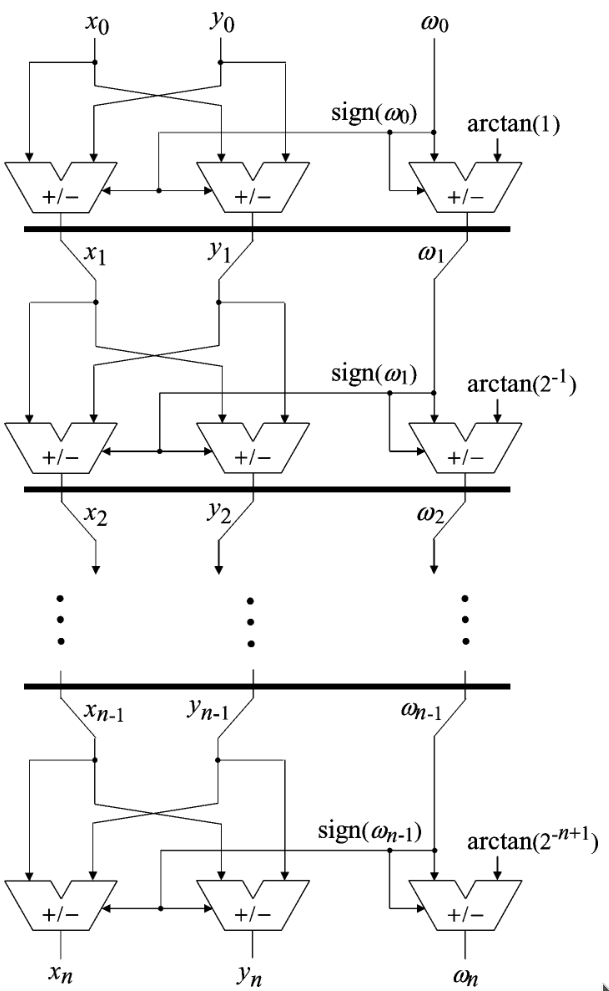
\includegraphics[width=0.50\textwidth]{archivos/CORDIC/2009-CORDIC_pipelined.png}
	\caption{\gls{cordic} convencional con \textit{pipelining}}
	\label{graf:2009-CORDIC_pipelined}
\end{figure}


\clearpage % Nueva página

Esta página también está en horizontal\\

\end{landscape} % Finaliza modo horizontal
\clearpage % Nueva página


Esta página está de nuevo en vertical\\
%%%%%%%%%%%%%%%%%%%%%%%%%%%%%%%%%%%%%%%%%%%%%%%%%%%%%%%%%%%%%%%%%%%%%%%%
% Plantilla TFG/TFM
% Escuela Politécnica Superior de la Universidad de Alicante
% Realizado por: Jose Manuel Requena Plens
% Contacto: info@jmrplens.com / Telegram:@jmrplens
%%%%%%%%%%%%%%%%%%%%%%%%%%%%%%%%%%%%%%%%%%%%%%%%%%%%%%%%%%%%%%%%%%%%%%%%




\chapter{Tablas de resultados}
\label{tablascompletas}
A continuación se muestran los datos y resultados obtenidos en el cálculo de coeficientes de corrección para la teoría revisada corregida (sección \ref{teoriarevisadacorregida}) en el caso de los recintos estudiados.

Se incluye en la tabla (las dos últimas columnas) la distancia donde se cortan el campo útil y el perjudicial, tanto para el caso de la simulación con EASE como para las curvas obtenidas mediante la teoría revisada corregida.
\begin{landscape}


\begin{table}[ht]
\centering
{\scalefont{0.65}
\begin{tabular}{@{}ccccccccccccccccc@{}}
\multicolumn{17}{c}{Fuente en el centro} \\ \toprule
\begin{tabular}[c]{@{}c@{}}Factor de\\ escala\end{tabular} & \begin{tabular}[c]{@{}c@{}}V\\ $m^3$\end{tabular} & \begin{tabular}[c]{@{}c@{}}S\\ $m^2$\end{tabular} & $\overline \alpha$ & $A_{\text{Eyring}}$ & \begin{tabular}[c]{@{}c@{}}Potencia\\ acústica\\ W\end{tabular} & Q & \begin{tabular}[c]{@{}c@{}}$T_{\text{Eyring}}$\\ s\end{tabular} & \begin{tabular}[c]{@{}c@{}}c\\ $m/s$\end{tabular} & \begin{tabular}[c]{@{}c@{}}Z\\ rayl\end{tabular} & $C_D$ & $\epsilon_E$ & $C_E$ & $\epsilon_L$ & $C_L$ & \begin{tabular}[c]{@{}c@{}}Cruce campos\\ teórico\\ m\end{tabular} & \begin{tabular}[c]{@{}c@{}}Cruce campos\\ EASE\\ m\end{tabular} \\ \midrule
0.5 & 62 & 128 & 0.118 & 16.517 & 0.00264 & 1 & 0.62 & 343.4 & 413.48 & 0.869 & -3.553 & 0.909 & 0.980 & 1.262 & - & - \\
0.6 & 107 & 184 & 0.118 & 23.900 & 0.00264 & 1 & 0.75 & 343.4 & 413.48 & 0.791 & -3.310 & 1.054 & 0.985 & 1.175 & - & - \\
0.7 & 170 & 251 & 0.118 & 32.534 & 0.00264 & 1 & 0.87 & 343.4 & 413.48 & 0.796 & -3.341 & 1.118 & 1.004 & 1.121 & - & - \\
0.8 & 253 & 328 & 0.118 & 42.420 & 0.00264 & 1 & 0.99 & 343.4 & 413.48 & 0.839 & -3.271 & 1.199 & 1.024 & 1.090 & - & 6.47 \\
0.9 & 361 & 415 & 0.118 & 53.681 & 0.00264 & 1 & 1.12 & 343.4 & 413.48 & 0.866 & -2.998 & 1.325 & 1.058 & 1.087 & 4.25 & 5.36 \\
1 & 495 & 512 & 0.118 & 66.320 & 0.00264 & 1 & 1.24 & 343.4 & 413.48 & 0.937 & -2.123 & 1.683 & 1.195 & 1.175 & 4.46 & 5.12 \\
1.1 & 659 & 619 & 0.118 & 80.209 & 0.00264 & 1 & 1.37 & 343.4 & 413.48 & 0.967 & -1.250 & 2.083 & 1.256 & 1.175 & 4.75 & 5.11 \\
1.2 & 855 & 737 & 0.118 & 95.475 & 0.00264 & 1 & 1.49 & 343.4 & 413.48 & 1.025 & -2.095 & 1.756 & 1.309 & 1.168 & 4.27 & 4.96 \\
1.3 & 1087 & 865 & 0.118 & 111.993 & 0.00264 & 1 & 1.62 & 343.4 & 413.48 & 1.028 & -0.338 & 2.579 & 1.336 & 1.141 & 5.10 & 5.27 \\
1.4 & 1358 & 1003 & 0.118 & 130.012 & 0.00264 & 1 & 1.74 & 343.4 & 413.48 & 1.028 & 1.200 & 3.559 & 1.351 & 1.118 & 5.67 & 5.58 \\
1.5 & 1670 & 1152 & 0.118 & 149.157 & 0.00264 & 1 & 1.86 & 343.4 & 413.48 & 1.019 & -1.176 & 2.334 & 1.373 & 1.101 & 5.03 & 5.46 \\
1.6 & 2027 & 1310 & 0.118 & 169.678 & 0.00264 & 1 & 1.99 & 343.4 & 413.48 & 1.018 & 1.154 & 3.693 & 1.381 & 1.077 & 5.97 & 5.89 \\
1.7 & 2431 & 1479 & 0.118 & 191.576 & 0.00264 & 1 & 2.11 & 343.4 & 413.48 & 1.012 & -1.776 & 2.014 & 1.422 & 1.074 & 4.63 & 5.20 \\
1.8 & 2885 & 1658 & 0.118 & 214.851 & 0.00264 & 1 & 2.24 & 343.4 & 413.48 & 1.017 & 1.746 & 4.321 & 1.423 & 1.051 & 6.53 & 6.35 \\
1.9 & 3394 & 1848 & 0.118 & 239.376 & 0.00264 & 1 & 2.36 & 343.4 & 413.48 & 1.017 & -0.425 & 2.944 & 1.477 & 1.059 & 5.87 & 6.15 \\
2 & 3958 & 2048 & 0.118 & 265.153 & 0.00264 & 1 & 2.49 & 343.4 & 413.48 & 1.017 & 0.087 & 3.182 & 1.486 & 1.045 & 6.03 & 6.09 \\ \bottomrule
\\
\multicolumn{17}{c}{Fuente en la esquina} \\ \toprule
\begin{tabular}[c]{@{}c@{}}Factor de\\ escala\end{tabular} & \begin{tabular}[c]{@{}c@{}}V\\ $m^3$\end{tabular} & \begin{tabular}[c]{@{}c@{}}S\\ $m^2$\end{tabular} & $\overline \alpha$ & $A_{\text{Eyring}}$ & \begin{tabular}[c]{@{}c@{}}Potencia\\ acústica\\ W\end{tabular} & Q & \begin{tabular}[c]{@{}c@{}}$T_{\text{Eyring}}$\\ s\end{tabular} & \begin{tabular}[c]{@{}c@{}}c\\ $m/s$\end{tabular} & \begin{tabular}[c]{@{}c@{}}Z\\ rayl\end{tabular} & $C_D$ & $\epsilon_E$ & $C_E$ & $\epsilon_L$ & $C_L$ & \begin{tabular}[c]{@{}c@{}}Cruce campos\\ teórico\\ m\end{tabular} & \begin{tabular}[c]{@{}c@{}}Cruce campos\\ EASE\\ m\end{tabular} \\ \midrule
0,5 & 62 & 128 & 0,118 & 16,517 & 0,00264 & 1 & 0,62 & 343,4 & 413,48 & 1,696 & -0,982 & 1,993 & 0,936 & 1,241 & - & - \\
0,6 & 107 & 184 & 0,118 & 23,900 & 0,00264 & 1 & 0,75 & 343,4 & 413,48 & 1,413 & -0,837 & 2,325 & 0,997 & 1,251 & - & - \\
0,7 & 170 & 251 & 0,118 & 32,534 & 0,00264 & 1 & 0,87 & 343,4 & 413,48 & 1,174 & -0,617 & 2,739 & 1,058 & 1,233 & - & - \\
0,8 & 253 & 328 & 0,118 & 42,420 & 0,00264 & 1 & 0,99 & 343,4 & 413,48 & 1,029 & -0,511 & 3,024 & 1,118 & 1,237 & - & 13,73 \\
0,9 & 361 & 415 & 0,118 & 53,681 & 0,00264 & 1 & 1,12 & 343,4 & 413,48 & 0,984 & -0,425 & 3,286 & 1,202 & 1,277 & 9,88 & 10,88 \\
1 & 495 & 512 & 0,118 & 66,320 & 0,00264 & 1 & 1,24 & 343,4 & 413,48 & 0,949 & -0,339 & 3,533 & 1,244 & 1,268 & 8,86 & 9,76 \\
1,1 & 659 & 619 & 0,118 & 80,209 & 0,00264 & 1 & 1,37 & 343,4 & 413,48 & 0,910 & -0,246 & 3,788 & 1,271 & 1,241 & 8,52 & 9,28 \\
1,2 & 855 & 737 & 0,118 & 95,475 & 0,00264 & 1 & 1,49 & 343,4 & 413,48 & 0,807 & -0,103 & 4,120 & 1,276 & 1,198 & 8,46 & 8,99 \\
1,3 & 1087 & 865 & 0,118 & 111,993 & 0,00264 & 1 & 1,62 & 343,4 & 413,48 & 0,809 & -0,022 & 4,369 & 1,275 & 1,152 & 8,59 & 9,00 \\
1,4 & 1358 & 1003 & 0,118 & 130,012 & 0,00264 & 1 & 1,74 & 343,4 & 413,48 & 0,815 & 0,139 & 4,768 & 1,273 & 1,117 & 8,90 & 9,16 \\
1,5 & 1670 & 1152 & 0,118 & 149,157 & 0,00264 & 1 & 1,86 & 343,4 & 413,48 & 0,883 & 0,084 & 4,790 & 1,274 & 1,084 & 8,95 & 9,22 \\
1,6 & 2027 & 1310 & 0,118 & 169,678 & 0,00264 & 1 & 1,99 & 343,4 & 413,48 & 0,927 & 0,140 & 5,006 & 1,297 & 1,074 & 9,17 & 9,36 \\
1,7 & 2431 & 1479 & 0,118 & 191,576 & 0,00264 & 1 & 2,11 & 343,4 & 413,48 & 0,943 & 0,209 & 5,232 & 1,313 & 1,061 & 9,38 & 9,52 \\
1,8 & 2885 & 1658 & 0,118 & 214,851 & 0,00264 & 1 & 2,24 & 343,4 & 413,48 & 0,981 & 0,427 & 5,798 & 1,323 & 1,047 & 10,00 & 9,93 \\
1,9 & 3394 & 1848 & 0,118 & 239,376 & 0,00264 & 1 & 2,36 & 343,4 & 413,48 & 0,954 & 0,394 & 5,787 & 1,325 & 1,028 & 9,94 & 9,89 \\
2 & 3958 & 2048 & 0,118 & 265,153 & 0,00264 & 1 & 2,49 & 343,4 & 413,48 & 0,970 & 0,539 & 6,218 & 1,335 & 1,019 & 10,39 & 10,22 \\ \bottomrule
\end{tabular}
}
\caption{Resultados con el aula OP/S003 sin mobiliario simulada con EASE.}
\label{tablacompletaop}
\end{table}


\begin{table}[ht]
\centering
{\scalefont{0.65}
\begin{tabular}{@{}ccccccccccccccccc@{}}
\multicolumn{17}{c}{Fuente en el centro} \\ \toprule
\begin{tabular}[c]{@{}c@{}}Factor de\\ escala\end{tabular} & \begin{tabular}[c]{@{}c@{}}V\\ $m^3$\end{tabular} & \begin{tabular}[c]{@{}c@{}}S\\ $m^2$\end{tabular} & $\overline \alpha$ & $A_{\text{Eyring}}$ & \begin{tabular}[c]{@{}c@{}}Potencia\\ acústica\\ W\end{tabular} & Q & \begin{tabular}[c]{@{}c@{}}$T_{\text{Eyring}}$\\ s\end{tabular} & \begin{tabular}[c]{@{}c@{}}c\\ $m/s$\end{tabular} & \begin{tabular}[c]{@{}c@{}}Z\\ rayl\end{tabular} & $C_D$ & $\epsilon_E$ & $C_E$ & $\epsilon_L$ &  $C_L$ & \begin{tabular}[c]{@{}c@{}}Cruce campos\\ teórico\\ m\end{tabular} & \begin{tabular}[c]{@{}c@{}}Cruce campos\\ EASE\\ m\end{tabular} \\ \midrule
0.5 & 29 & 68 & 0.109 & 8.083 & 0.00264 & 1 & 0.59 & 343.4 & 413.48 & 0.821 & -5.706 & 0.589 & 1.164 & 1.238 & - & - \\
0.6 & 49 & 98 & 0.109 & 11.662 & 0.00264 & 1 & 0.70 & 343.4 & 413.48 & 0.869 & -5.755 & 0.664 & 0.964 & 0.945 & - & - \\
0.7 & 78 & 133 & 0.109 & 15.819 & 0.00264 & 1 & 0.82 & 343.4 & 413.48 & 0.950 & -5.917 & 0.708 & 0.888 & 0.850 & - & - \\
0.8 & 117 & 174 & 0.109 & 20.668 & 0.00264 & 1 & 0.94 & 343.4 & 413.48 & 0.966 & -5.047 & 0.863 & 0.976 & 0.920 & - & - \\
0.9 & 166 & 220 & 0.109 & 26.210 & 0.00264 & 1 & 1.05 & 343.4 & 413.48 & 0.966 & -3.872 & 1.077 & 0.986 & 0.922 & - & 4.48 \\
1 & 228 & 272 & 0.101 & 29.797 & 0.00264 & 1 & 1.27 & 343.4 & 413.48 & 0.965 & -3.895 & 1.073 & 1.081 & 0.843 & 3.80 & 4.03 \\
1.1 & 304 & 329 & 0.109 & 39.142 & 0.00264 & 1 & 1.29 & 343.4 & 413.48 & 0.964 & -4.869 & 1.036 & 0.962 & 0.882 & 3.27 & 4.01 \\
1.2 & 394 & 391 & 0.109 & 46.532 & 0.00264 & 1 & 1.40 & 343.4 & 413.48 & 0.963 & -3.646 & 1.257 & 0.921 & 0.852 & 3.28 & 3.78 \\
1.3 & 501 & 459 & 0.109 & 54.615 & 0.00264 & 1 & 1.52 & 343.4 & 413.48 & 0.962 & -3.505 & 1.298 & 1.004 & 0.896 & 3.11 & 3.56 \\
1.4 & 626 & 532 & 0.109 & 63.390 & 0.00264 & 1 & 1.64 & 343.4 & 413.48 & 0.961 & -2.162 & 1.665 & 1.081 & 0.929 & 3.54 & 3.84 \\
1.5 & 770 & 611 & 0.109 & 72.743 & 0.00264 & 1 & 1.76 & 343.4 & 413.48 & 0.961 & -0.123 & 2.277 & 1.047 & 0.903 & 4.00 & 4.06 \\
1.6 & 934 & 695 & 0.109 & 82.672 & 0.00264 & 1 & 1.87 & 343.4 & 413.48 & 0.960 & -2.655 & 1.630 & 1.077 & 0.908 & 3.47 & 3.85 \\
1.7 & 1121 & 785 & 0.109 & 93.411 & 0.00264 & 1 & 1.99 & 343.4 & 413.48 & 0.959 & -0.943 & 2.116 & 1.119 & 0.917 & 3.93 & 4.10 \\
1.8 & 1330 & 880 & 0.109 & 104.726 & 0.00264 & 1 & 2.11 & 343.4 & 413.48 & 0.961 & 1.478 & 3.101 & 1.137 & 0.914 & 4.63 & 4.58 \\
1.9 & 1565 & 980 & 0.109 & 116.619 & 0.00264 & 1 & 2.22 & 343.4 & 413.48 & 0.958 & 0.890 & 2.782 & 1.160 & 0.913 & 4.43 & 4.43 \\
2 & 1825 & 1086 & 0.109 & 129.205 & 0.00264 & 1 & 2.34 & 343.4 & 413.48 & 0.957 & -0.239 & 2.493 & 1.179 & 0.911 & 4.38 & 4.48 \\ \bottomrule
\\
\multicolumn{17}{c}{Fuente en la esquina} \\ \toprule
\begin{tabular}[c]{@{}c@{}}Factor de\\ escala\end{tabular} & \begin{tabular}[c]{@{}c@{}}V\\ $m^3$\end{tabular} & \begin{tabular}[c]{@{}c@{}}S\\ $m^2$\end{tabular} & $\overline \alpha$ & $A_{\text{Eyring}}$ & \begin{tabular}[c]{@{}c@{}}Potencia\\ acústica\\ W\end{tabular} & Q & \begin{tabular}[c]{@{}c@{}}$T_{\text{Eyring}}$\\ s\end{tabular} & \begin{tabular}[c]{@{}c@{}}c\\ $m/s$\end{tabular} & \begin{tabular}[c]{@{}c@{}}Z\\ rayl\end{tabular} & $C_D$ & $\epsilon_E$ & $C_E$ & $\epsilon_L$ & $C_L$ & \begin{tabular}[c]{@{}c@{}}Cruce campos\\ teórico\\ m\end{tabular} & \begin{tabular}[c]{@{}c@{}}Cruce campos\\ EASE\\ m\end{tabular} \\ \midrule
0.5 & 29 & 68 & 0.109 & 8.083 & 0.00264 & 1 & 0.59 & 343.4 & 413.48 & 1.355 & -2.543 & 1.052 & 0.960 & 0.933 & - & - \\
0.6 & 49 & 98 & 0.109 & 11.662 & 0.00264 & 1 & 0.70 & 343.4 & 413.48 & 1.280 & -2.392 & 1.232 & 0.854 & 0.821 & - & - \\
0.7 & 78 & 133 & 0.109 & 15.819 & 0.00264 & 1 & 0.82 & 343.4 & 413.48 & 1.201 & -2.310 & 1.370 & 0.901 & 0.865 & - & - \\
0.8 & 117 & 174 & 0.109 & 20.668 & 0.00264 & 1 & 0.94 & 343.4 & 413.48 & 1.003 & -2.156 & 1.534 & 0.972 & 0.923 & - & - \\
0.9 & 166 & 220 & 0.109 & 26.210 & 0.00264 & 1 & 1.05 & 343.4 & 413.48 & 1.024 & -2.081 & 1.654 & 0.987 & 0.923 & - & - \\
1 & 228 & 272 & 0.101 & 29.797 & 0.00264 & 1 & 1.27 & 343.4 & 413.48 & 1.046 & -2.209 & 1.618 & 1.084 & 0.839 & 6.72 & 8.16 \\
1.1 & 304 & 329 & 0.109 & 39.142 & 0.00264 & 1 & 1.29 & 343.4 & 413.48 & 0.941 & -1.709 & 2.008 & 0.990 & 0.890 & 5.99 & 7.16 \\
1.2 & 394 & 391 & 0.109 & 46.532 & 0.00264 & 1 & 1.40 & 343.4 & 413.48 & 0.937 & -1.848 & 1.992 & 0.992 & 0.878 & 5.31 & 6.49 \\
1.3 & 501 & 459 & 0.109 & 54.615 & 0.00264 & 1 & 1.52 & 343.4 & 413.48 & 0.924 & -1.541 & 2.229 & 0.993 & 0.871 & 5.39 & 6.24 \\
1.4 & 626 & 532 & 0.109 & 63.390 & 0.00264 & 1 & 1.64 & 343.4 & 413.48 & 0.905 & -1.665 & 2.208 & 0.982 & 0.856 & 5.08 & 5.91 \\
1.5 & 770 & 611 & 0.109 & 72.743 & 0.00264 & 1 & 1.76 & 343.4 & 413.48 & 0.871 & -1.597 & 2.304 & 0.966 & 0.839 & 5.10 & 5.83 \\
1.6 & 934 & 695 & 0.109 & 82.672 & 0.00264 & 1 & 1.87 & 343.4 & 413.48 & 0.895 & -1.497 & 2.417 & 0.949 & 0.819 & 5.22 & 5.85 \\
1.7 & 1121 & 785 & 0.109 & 93.411 & 0.00264 & 1 & 1.99 & 343.4 & 413.48 & 0.923 & -0.861 & 2.952 & 0.924 & 0.802 & 6.03 & 6.41 \\
1.8 & 1330 & 880 & 0.109 & 104.726 & 0.00264 & 1 & 2.11 & 343.4 & 413.48 & 0.922 & -1.299 & 2.655 & 0.911 & 0.789 & 5.54 & 6.00 \\
1.9 & 1565 & 980 & 0.109 & 116.619 & 0.00264 & 1 & 2.22 & 343.4 & 413.48 & 0.954 & -1.220 & 2.758 & 0.891 & 0.774 & 5.72 & 6.12 \\
2 & 1825 & 1086 & 0.109 & 129.205 & 0.00264 & 1 & 2.34 & 343.4 & 413.48 & 0.970 & -1.017 & 2.965 & 0.866 & 0.757 & 6.06 & 6.41 \\ \bottomrule
\end{tabular}
}
\caption{Resultados con el aula EP/0-26M sin mobiliario simulada con EASE.}
\label{tablacompletaeps}
\end{table}



\end{landscape}


%%%%%%%%%%%%%%%%%%%%%%%%%%%%%%%%%%%%%%%%%%%%%%%%%%%%%%%%%%%%%%%%%%%%%%%%%
% Plantilla TFG/TFM
% Escuela Politécnica Superior de la Universidad de Alicante
% Realizado por: Jose Manuel Requena Plens
% Contacto: info@jmrplens.com / Telegram:@jmrplens
%%%%%%%%%%%%%%%%%%%%%%%%%%%%%%%%%%%%%%%%%%%%%%%%%%%%%%%%%%%%%%%%%%%%%%%%

% Ejemplo de inclusión de páginas de un PDF

\chapter{Importar PDF}

A continuación se muestra una página importada de un PDF externo. Observar los comentarios en el código de este anexo para más información. También puedes leer el manual con todas las opciones en \url{http://osl.ugr.es/CTAN/macros/latex/contrib/pdfpages/pdfpages.pdf}.

\includepdf[pages={1}]{archivos/ES_a_DF7_Agg_Alicante.pdf}

% Para incluir una página:
% [pages={0}] % Donde '0' es el número de la pagina del PDF que se quiere incluir

% Para incluir varias páginas consecutivas
% [pages={1-4}] % Con estos valores importa de la página 1 a la 4.

% Para incluir varias páginas salteadas
% [pages={1,4,7,10}] % Incluye las páginas 1,4,7 y 10

% Para incluir todo el documento PDF
% [pages=-]

% Si ademas de pages=... se incluye landscape, se importa en horizontal
% [pages{1},landscape]

\end{document}
